%!TEX TS-program = XeLaTeX
% \newcommand{\path}{/Users/yuchen/Documents/Research/PaperEngine}

\documentclass[lang=cn, cm, 10pt, scheme=chinese, bibend=bibtex, citestyle=alphabetic, bibstyle=alphabetic]{elegantbook}

\title{密码科学技术丛书}
\subtitle{公钥加密的设计方法}

\author{陈宇 \& 秦宝东}
\institute{山东大学 \& 西安邮电大学}
\date{}
\version{0.1}
\extrainfo{微言大义~高屋建瓴}

\cover{天坛.png}

% 本文档命令
\elegantnewtheorem{claim}{断言}{thmstyle}{exfancy}
\elegantnewtheorem{remark}{注记}{prostyle}{exfancy}
\elegantnewtheorem{construction}{构造}{defstyle}{exfancy}
\elegantnewtheorem{thinking}{思考}{prostyle}{exfancy}

\usepackage{array}
\newcommand{\ccr}[1]{\makecell{{\color{#1}\rule{1cm}{1cm}}}}

% 修改标题页的橙色带
\definecolor{customcolor}{RGB}{32,178,170}
\colorlet{coverlinecolor}{customcolor}
\usepackage{cprotect}

\setcounter{tocdepth}{3}

\addbibresource[location=local]{mycrypto.bib} % 参考文献,不要删除

% import customized commands
\usepackage{caption}
\usepackage{latexsym}
\usepackage{amsmath, amssymb, amsfonts}
\usepackage{mathrsfs}
\usepackage{graphicx}
\usepackage{xcolor}
\usepackage{colortbl}
\usepackage{soul}
\usepackage{enumerate}
\usepackage{enumitem}
\usepackage{setspace}
\usepackage{framed}
\usepackage{boxedminipage}
\usepackage{cancel,siunitx}
\usepackage{amssymb}% http://ctan.org/pkg/amssymb
\usepackage{pifont}% http://ctan.org/pkg/pifont
\usepackage{makecell}
\usepackage{tabularx}
\usepackage{multirow}
\usepackage{threeparttable}
\usepackage[ruled,vlined,linesnumbered]{algorithm2e}
\usepackage{url}
\usepackage{float}
\usepackage{mdframed}
\usepackage[normalem]{ulem} % 批注
\usepackage{autobreak}

\usepackage{adjustbox}
\usepackage{dashbox}


\usepackage{tikz}     % 绘图包
\usetikzlibrary{calc, matrix, patterns, backgrounds, arrows, shapes, snakes, circuits, circuits.logic.US, 
chains, fit, decorations, intersections, positioning}

\tikzset{
    shapenode/.style = {draw, rectangle, fill=none, auto, node distance=0em, font=\normalsize}, 
    roundnode/.style = {draw, rectangle, rounded corners=0.5em, inner sep = 0.2em, 
      node distance=0em, minimum height=1.5em},
    rectanglenode/.style = {draw, rectangle, inner sep = 0em, node distance=0em},
    textnode/.style  = {draw=none, fill=none, rectangle, minimum size=0cm, inner sep = 0em, 
      auto, node distance=0em, font=\normalsize},
    smalltextnode/.style  = {draw=none, fill=none, rectangle, minimum size=0.5cm, auto, node distance=0em, font=\small},
    circlenode/.style = {circle, draw, auto, inner sep = 0em, node distance=0em}, 
    ellipsenode/.style = {draw, ellipse, inner sep = 0em, node distance=0em, minimum height=0em, minimum width=0em},
    dotnode/.style = {draw, fill=black, circle, auto, minimum size=0.2em, inner sep = 0em, node distance=0em},  
    connect/.style = {black,->},
    implies/.style={double,double equal sign distance,-implies}, 
    every text node part/.style={align=center}
}

% define the colors
\definecolor{lightmidnightblue}{rgb}{0.2, 0.2, 0.7}
\definecolor{darkgreen}{rgb}{0.0,0.5,0.0}

\newcommand{\blue}[1]{{\color{blue} #1}}
\newcommand{\cyan}[1]{{\color{cyan} #1}}
\newcommand{\purple}[1]{{\color{purple} #1}}
\newcommand{\yellow}[1]{{\color{yellow} #1}}
\newcommand{\darkred}[1]{{\color{darkred} #1}}
\newcommand{\gray}[1]{{\color{gray} #1}}
\newcommand{\red}[1]{{\color{red} #1}}
\newcommand{\green}[1]{{\color{green}#1}}
\newcommand{\magenta}[1]{{\color{magenta} #1}}
\newcommand{\black}[1]{{\color{black} #1}}
\newcommand{\orange}[1]{{\color{orange} #1}}
\newcommand{\mdblue}[1]{{\color{lightmidnightblue} #1}}

\colorlet{lightgray}{gray!20}
\colorlet{darkgray}{gray!100}

% define notions
\renewcommand{\P}{\mathbf{P}}
\newcommand{\NP}{\mathbf{NP}}
\newcommand{\coNP}{\textup{co-}\mathbf{NP}}

% define shorthands
\newcommand{\define}{\stackrel{\textup{def}}{=}}

\newcommand{\iO}{i\mathcal{O}}
\newcommand{\diO}{di\mathcal{O}}
\newcommand{\sample}{\xleftarrow{\textup{\tiny R}}}
\newcommand{\expect}{\mathbb{E}}
\newcommand{\entropy}{\mathsf{H}}
\newcommand{\minentropy}{\mathsf{H}_\infty}
\newcommand{\avminentropy}{\tilde{\mathsf{H}}_\infty}
\newcommand{\AdvA}{\mathsf{Adv}_\mathcal{A}}
\newcommand{\AdvB}{\mathsf{Adv}_\mathcal{B}}

\newcommand{\outV}{\text{out}_V}
\newcommand{\viewV}{\text{view}_V}
\newcommand{\viewVstar}{\text{view}_{V^*}}

\newcommand{\Oderive}{\mathcal{O}_\mathsf{derive}^\Phi}
\newcommand{\Oinv}{\mathcal{O}_\mathsf{inv}}
\newcommand{\Oleak}{\mathcal{O}_\mathsf{leak}(\cdot)}
\newcommand{\Ovefy}{\mathcal{O}_\mathsf{vefy}(\cdot,\cdot)}
\newcommand{\Otag}{\mathcal{O}_\mathsf{tag}(\cdot)}
\newcommand{\Osign}{\mathcal{O}_\mathsf{sign}}
\newcommand{\Odecrypt}{\mathcal{O}_\mathsf{decrypt}}
\newcommand{\Odecaps}{\mathcal{O}_\mathsf{decaps}}
\newcommand{\OregH}{\mathcal{O}_\mathsf{regH}}
\newcommand{\OregC}{\mathcal{O}_\mathsf{regC}}
\newcommand{\Oreveal}{\mathcal{O}_\mathsf{reveal}}
\newcommand{\Oibedecaps}{\mathcal{O}_\mathsf{decaps}(\cdot, \cdot)}
\newcommand{\Osim}{\mathcal{O}_\mathsf{sim}}
\newcommand{\Oenc}{\mathcal{O}_\mathsf{enc}}
\newcommand{\Oext}{\mathcal{O}_\mathsf{ext}}
\newcommand{\Oeval}{\mathcal{O}_\mathsf{eval}}
\newcommand{\Oconstrain}{\mathcal{O}_\mathsf{constrain}}
\newcommand{\Oevalempty}{\mathcal{O}_\mathsf{eval}(\$)}

\newcommand{\Oracle}{\mathcal{O}}
\newcommand{\TBA}{\blue{To be add more ...}}

\newcommand{\poly}{\textup{poly}}
\newcommand{\polylog}{\textup{polylog}}
\newcommand{\loglog}{\textup{loglog}}
% \newcommand{\MA}{\mathbf{MA}}
% \newcommand{\PSAPCE}{\mathbf{PSPACE}}
% \newcommand{\NEXT}{\mathbf{NEXT}}


\newcommand{\cmark}{\ding{51}}%
\newcommand{\xmark}{\ding{55}}%
\newcommand{\redcross}{{\tikz[x=1.4ex, y=1.4ex, line width=.2ex, red] \draw (0,0) -- (2,2) (0,2) -- (2,0);}}%

\newcommand{\redul}{\bgroup\markoverwith{\textcolor{red}{\rule[-0.5ex]{2pt}{0.4pt}}}\ULon} % 红色下划线
\newcommand{\blueul}{\bgroup\markoverwith{\textcolor{blue}{\rule[-0.5ex]{2pt}{0.4pt}}}\ULon} % 蓝色下划线
\newcommand{\blackul}{\bgroup\markoverwith{\textcolor{black}{\rule[-0.5ex]{2pt}{0.4pt}}}\ULon} % 黑色下划线


\newcommand{\qed}{\hfill \ensuremath{\Box}}

%%%%By QIN Baodong===Begin
\newcommand{\F}{\mathcal{F}}
\newcommand{\Faff}{\mathcal{F}_{\text{aff}}}
\newcommand{\Fpolyd}{\mathcal{F}_{\text{poly}}^{d}}
\newcommand{\AIAE}{\mathsf{AIAE}}
\newcommand{\prmAIAE}{pp_{\text{AIAE}}}
\newcommand{\KAIAE}{\mathcal{K}_{\text{AIAE}}}
\newcommand{\gra} {\textcolor[RGB]{180, 180, 180}}
\definecolor{gra}{RGB}{220, 220, 220}
\newcommand{\grabox}{\colorbox{gra}}
\newcommand{\hpt}{\hspace{1pt}}
%\newcommand{\dslash}{/\hspace{-2pt}/\hspace{2pt}}
%%%%===End


\begin{document}

\maketitle

\frontmatter
\chapter{前言}
本书是在``2017-2019中国科学院大学研究生暑期课程''和``2022北京大学应用数学专题讲习班''的讲义基础上, 结合多年在公钥加密方面的研究成果编写而成. 
目的是尽快引导读者到达公钥加密这一极重要的现代密码学领域, 力求从高屋建瓴的视角介绍公钥加密的设计方法, 对重要的思想剥丝抽茧、对关键的技术条分缕析. 
写作过程中根据教学和研究经历感悟对内容做了取舍和精简, 参阅了国际顶级会议期刊的前沿论文, 也融入了作者的独立思考.   

计算机网络技术的飞速发展引发了人类社会组织形态的根本性变革, 从集中式迁移为分布式, ``海内存知己, 天涯若比邻''从诗歌意象走进现实世界. 
面向分布式环境下的隐私保护需求, 1976年Diffie和Hellman开创了现代密码学的新方向—公钥密码学. 
迄今为止的半个多世纪以来, 公钥密码学一直处于最活跃的前沿, 引领驱动了密码学的研究进展, 极大丰富了密码学的学科内涵. 
公钥加密作为公钥密码学最重要的分支, 在理论方面孕育了可证明安全方法、将各类数学困难问题纳入工具库、启发了一系列密码原语和重要概念, 
已有多项历史性成果获得Turing奖和G\"odel奖; 在应用方面则是各类网络通信安全协议的核心组件, 时刻保护着公开信道上消息传输的机密性. 

近期, 公钥加密仍处于快速发展阶段, 在安全性方面, 各类超越传统语义安全的高级安全属性研究已经日趋成熟, 基于复杂性弱假设的细粒度安全的研究正在兴起; 
在功能性方面, 函数加密的研究方兴未艾, 全同态加密的研究如火如荼. 我们已经有幸见证了公钥加密之旅的美妙风景, 但还有更广袤深邃的领域待探索征服. 

公钥加密历经多年发展, 各类方案层出不穷, 相关概念定义繁多, 因此想深入学习的读者往往会感觉陷入书山文海, 难识庐山真面目. 
本书试图快速引导读者登高俯瞰, 将公钥加密的设计方法尽收眼底, 达到万变不离其宗的认知. 
为此, 本书的内容偏重基于一般假设的通用构造. 这样的选择有诸多好处, 从理论角度, 通用构造剥离了不必要的细节、凸显了核心要素, 从而更容易洞察公钥加密的本质和复杂性下界; 
从实际角度, 通用构造可以启发更多的具体构造, 可根据安全或应用的需求灵活选择新的困难假设给出实例化方案. 

本书的第一章简述了公钥加密的发展历程, 第二章介绍了准备知识, 为后续章节做好铺垫. 
第三章回顾经典的公钥加密方案, 方便读者先获得具象的认识, 预备一些重要的例子. 
第四章是核心部分, 从各类密码组件出发展示了公钥加密的通用构造, 并在最后获得更高阶的抽象, 与对称加密的构造相互呼应、完美契合. 
第五章和第六章分别从安全性增强和功能性扩展两个维度介绍公钥加密的重要成果和前沿进展. 
第七章简介了公钥加密的标准化与工程实践, 打通理论与实践的最后一公里. 

书中有不少看似不起眼的注记, 它们大多来源于作者科研过程中的心得体会, 领悟其中蕴含的思辨方式之后或许能看到更美的风景. 
总的来说, 切实掌握本书的内容之后, 可使读者进入可证明安全密码学的新层次, 为进一步的研究打好基础. 

%密码科学技术国家实验室对本书的出版给予了极大支持, 作者深表感谢. 
作者感谢山东大学王美琴教授、王伟嘉教授在本书在写作过程给予的极大支持. 
作者也借此机会感谢清华大学王小云院士、中国科学院林东岱研究员、邓燚研究员和上海交通大学的郁昱教授、刘胜利教授多年以来的给予的鼓励和指点. 
最后, 感谢家人们的默默支持, 没有你们的全情支持, 我们不可能完成此书.   

由于水平有限, 时间紧迫, 定有许多不当之处. 诚恳欢迎批评指正. \\*[2em]

\hfill 陈宇 \& 秦宝东 \\

\hfill 2023年夏   % 前言章节 preface.tex

\tableofcontents


\mainmatter

\chapter*{前言}\normalsize
  \addcontentsline{toc}{chapter}{前言}


\chapter{公钥加密的概述}
\section{背景与起源}

密码的历史甚至早于文字的出现. 密码的历史进程大概可以分为以下几个阶段: 
\begin{itemize}
	\item 古典阶段: 
	\item 现代阶段: Shannon和DES 
	\item Diffie-Hellman的密码学新方向.   
\end{itemize}
\section{发展历程简介}
目前的设想是从两个维度梳理公钥加密的发展历史: 功能性的丰富和安全性的增强. 

自Diffie和Hellman的划时代论文~\cite{DH-IEEE-IT-1976}后, 
公钥密码学的发展一日千里、日新月异, 热潮持续至今, 始终是现代密码学的核心和重要技术的摇篮. 

公钥密码的发展大体可以分为两条主线: 一条是安全性的增强, 从最初的直觉安全演进到严格健壮的语义安全, 
再到不可区分选择密文安全和各类超越传统安全模型的高级安全性, 如抗泄漏安全、抗篡改安全和消息依赖密钥安全; 
另一条是功能性的丰富, 从最初的一对一加解密到基于身份加密, 再到属性加密乃至极致泛化的函数加密. 

\subsection{安全性增强}
最初的RSA PKE只满足朴素单向安全. 
Goldwasser和Micali思考了公钥加密应该满足何种最低安全性这一问题, 提出了严格的安全模型, 设计了首个可证明安全的公钥加密方案Goldwasser-Micali PKE. 



\subsection{功能性丰富}
将加上与易红旭和王煜宇共同撰写的综述

\chapter{准备知识}
\section{符号与记号}
对于正整数$n$, 用$[n]$表示集合$\{1, \dots, n\}$.
对于集合$X$, $|X|$表示其大小, $x \sample X$表示从$X$中均匀采样$x$, 
$U_X$表示$X$上的均匀分布. 
如果一个概率算法的运行时间是关于输入规模$n$的多项式函数$\mathsf{poly}(n)$, 则称其是概率多项式时间的算法, 
简记为(probabilistic polynomial time, PPT).
令$\mathcal{A}$是一个随机算法, $z \leftarrow \mathcal{A}(x;r)$
表示$\mathcal{A}$在输入为$x$和随机带为$r$时输出$z$, 当上下文明确时, 常隐去随机带$r$简记为
$z \leftarrow \mathcal{A}(x)$.  
令$f(\cdot)$是关于$n$的函数, 如果对于任意的多项式$p(\cdot)$均存在常数$c$使得$n > c$时
总有$f(n) < 1/p(n)$成立, 则称$f$是关于$n$的可忽略函数, 记为$\mathsf{negl}(n)$.  
在本书中, $\kappa \in \mathbb{N}$表示计算安全参数, $\lambda \in \mathbb{N}$表示统计安全参数. 
令$X = \{X_k\}_{k \in \mathbb{N}}$和$Y = \{Y_k\}_{k \in \mathbb{N}}$
是两个由$k$索引的分布簇, 如果$X$和$Y$之间的统计距离是关于$\lambda$的可忽略函数, 
则称$X$和$Y$统计不可区分, 记为$X \approx_s Y$; 
如果任意PPT敌手区分$X$和$Y$的优势函数为$\mathsf{negl}(\kappa)$, 则称$X$和$Y$计算不可区分, 记为$X \approx_c Y$. 


对于实数$x \in \mathbb{R}$, 令$\lfloor x \rfloor$表示$x$的下取整, 
$\lfloor x \rceil := \lfloor x + 1/2\rfloor$表示与$x$最接近的整数.

令$F$是带密钥的函数, $F_k(x)$表示函数$F$在密钥$k$控制下对$x$的求值, 也常记作$F(k, x)$.  

\begin{table}[H]
\begin{center}
\caption{缩略词及其含义对照表}
\begin{tabular}{ccc}
\hline
缩略词   & 英文表达 & 中文含义\\
\hline
CPA     & chosen-plaintext attack  		& 选择明文攻击\\
CCA     & chosen-ciphertext attack 		& 选择密文攻击\\
PKE     & public-key encryption    		& 公钥加密方案\\
--      & hardcore function        		& 硬核函数\\ 
--      & hardcore predicate       		& 硬核谓词\\  
--      & oracle                   		& 谕言机\\
--      & one-way trapdoor function 	& 单向陷门函数\\
\hline
\end{tabular}
\end{center}
\end{table}



\section{可证明安全方法}

\begin{quote}
Talk is cheap. Show me the code.\\
\hspace*{\fill} --- Linus Torvalds 
\end{quote}

长久以来, 密码方案的安全性分析没有系统标准的方式, 传统方式由密码分析者通过尝试各类攻击来检验密码方案的安全性. 
容易看出, 传统的分析方式存在以下局限: 
(1) 分析结果严重依赖分析者的个人能力(如细致的观察和敏锐的直觉); (2) 分析者难以穷尽所有可能的攻击. 
因此, 绝大多数古典密码陷入``设计—攻破—修补—攻破''的循环往复怪圈, 难以称之为真正的科学. 

直到上世纪八十年代, Goldwasser和Micali~\cite{GM-STOC-1982}借鉴计算复杂性理论的归约技术, 开创了可证明安全方法. 
从此, 密码方案的安全性分析手段由反向攻击转为正向证明, 安全性由``声称安全''变为``可证安全'', 密码学也从此由艺术蝶变为真正的科学. 

简言之, 可证明安全方法的核心是以下三要素组成: 
\begin{itemize}
\item \textbf{精确的安全模型:} 通常由攻击者和挑战者之间的交互式游戏进行刻画, 如图~\ref{figure:security-model}所示, 包括: 
\begin{itemize}
	\item 敌手的计算能力: 常见的有概率多项式时间和指数时间
	\item 敌手能够获取的信息, 包括:
	\begin{enumerate}
		\item 固定信息: 如方案的公开参数等公开信息
		\item 非固定信息: 在攻击过程中获得的信息, 形式化为访问相应谕言机获得的输出
	\end{enumerate}
    \item 敌手的攻击效果: 以加密方案为例, 敌手恢复密钥和恢复明文是不同的攻击效果
\end{itemize}

\begin{figure}[!hbtp]
\begin{center}
\begin{tikzpicture}
\node[textnode, name=A] {敌手$\mathcal{A}$}; 
\node[rectanglenode, name=scheme, right of = A, xshift=20em, minimum height=3em, minimum width=6em, fill=blue!30] 
	{密码方案$\mathcal{E}$};  
\node[textnode, name=C, right of=scheme, xshift=6em] {挑战者$\mathcal{CH}$}; 

\draw ($(A.east)+(0em, 2em)$) edge[->] ($(scheme.west)+(0em, 2em)$);
\draw ($(A.east)+(0em, 0em)$) edge[densely dashed] ($(scheme.west)+(0em, 0em)$);
\draw ($(A.east)+(0em, -2em)$) edge[<-] ($(scheme.west)+(0em, -2em)$); 

\node[textnode, name=Adv, below of = A, xshift= 10em, yshift=-6em] {$\mathsf{Adv}_\mathcal{A}(\kappa) = |\Pr[S] - \Pr[T]|$}; 
\end{tikzpicture}
\end{center}
\caption{安全模型}\label{figure:security-model}
\end{figure}
令事件$S$表示敌手攻击成功这一事件, $t$表示某固定的基准优势(如区分类游戏定义为$1/2$, 搜索性游戏定义为$0$), 
定义$\mathcal{A}$的优势函数为$\mathsf{Adv}_\mathcal{A}(\kappa) = |\Pr[S] - t|$, 
其中$S$所在的概率空间由$\mathcal{A}$和$\mathcal{CH}$的随机带确定. 
如果对于所有PPT敌手$\mathcal{A}$, $\mathsf{Adv}_\mathcal{A}(\kappa)$均是关于安全参数$\kappa$的可忽略函数, 
则称密码方案$\mathcal{E}$在既定的安全模型下是安全的. 

\item \textbf{清晰的困难性假设}
\item \textbf{严格的归约式证明:} 通过反证式论证将方案的安全性归结到困难性假设. 
\end{itemize}  

图~\ref{figure:reduction-proof}是归约式证明的交换图表. 归约式证明的步骤如下: 
\begin{enumerate}
\item 假设存在PPT的敌手$\mathcal{A}$在既定安全模型下针对密码方案$\mathcal{E}$具有不可忽略的优势$\epsilon_1(\kappa)$; 
\item 利用$\mathcal{A}$的能力, 构建PPT的算法$\mathcal{B}$以不可忽略的优势$\epsilon_2(\kappa)$打破困难问题. 
	这里$\mathcal{R}$通常以扮演敌手$\mathcal{A}$的挑战者的方式调用$\mathcal{A}$, 因此也常称$\mathcal{R}$是模拟算法或归约算法. 
	$\mathcal{R}$调用敌手$\mathcal{A}$的方式又可细分为两类: 
	\begin{itemize}
		\item 黑盒方式: $\mathcal{R}$以黑盒的方式调用$\mathcal{A}$, 从算法的角度理解就是$\mathcal{R}$以$\mathcal{A}$作为子程序调用. 
			黑盒方式实质上证明了比所需更强的结果, 即$\exists \mathcal{R} ~ \forall \mathcal{A}$. 
			此类证明最为常见, 被称为黑盒归约(black-box reduction)或者一致归约(universal reduction). 

		\item 非黑盒方式: $\mathcal{R}$以非黑盒的方式调用$\mathcal{A}$, 充分利用了$\mathcal{A}$的个体信息, 如算法结构、运行时间等. 
			这类证明是完全契合可证明安全思想的, 即$\forall \mathcal{A} ~ \exists \mathcal{R}$. 
			此类证明相对少见, 被称为个体归约(individual reduction)~\cite{Deng-EUROCRYPT-2017}, 常可以突破黑盒归约下的安全性下界.  
	\end{itemize}
\end{enumerate}

\begin{figure}[!hbtp]
\begin{center}
\begin{tikzpicture}
\node[textnode, name=A] {$\mathcal{A}(t_1, \epsilon_1)$}; 
\node[rectanglenode, name=scheme, right of = A, xshift=20em, minimum height=3em, minimum width=6em, fill=blue!30] {密码方案};  
\draw (A) edge[->] node[midway, fill=white] {攻破} (scheme); 

\node[textnode, name=R, below of = A, yshift=-6em] {$\mathcal{R}(t_2, \epsilon_2)$};
\node[rectanglenode, name=assumption, right of = R, xshift=20em, minimum height=3em, minimum width=6em, 
	fill=gray!30] {困难性假设};    
\draw (R) edge[->] node[midway, fill=white] {攻破} (assumption); 

\draw (assumption) edge[->] (scheme); 
\draw (A) edge[->] (R);
\end{tikzpicture}
\end{center}
\caption{归约式证明的交换图表}\label{figure:reduction-proof}
\end{figure}

上述两步归约式论证的逻辑是: 构造出的算法$\mathcal{R}$与困难假设相矛盾, 因此不存在算法$\mathcal{R}$, 进而得出$\mathcal{A}$不存在的结论. 

\begin{trivlist}
\item \textbf{安全性强弱.} 在明确可证明安全方法后, 密码方案的强弱可以根据三要素的强弱定性分析: 
\begin{itemize}
	\item 安全模型的强弱: 敌手的计算能力越强大、获得的信息越多、攻击的效果越弱, 则所确定的安全模型越强, 反之越弱. 
	\item 困难假设的强弱: 通常搜索类假设强于判定类假设, 平均情形(average-case)假设强于最坏情形(worst-case)假设. 
	\item 归约质量的优劣: 笼统的说, $(t_2, \epsilon_2)$越接近$(t_1, \epsilon_1)$, 归约的质量越高. 
		在归约算法的运行时间和优势函数两个指标中, 通常更关注后者. 定义归约松紧因子$r = \epsilon_2/\epsilon_1$, 
		如果$r$是一个常数, 称归约是紧的; 如果$r$是一个可察觉的函数(noticeable function), 称归约多项式松弛的, 归约有效; 
		如果$r$是一个可忽略函数, 称归约超多项式松弛, 归约无效.  
\end{itemize}
\end{trivlist}

\begin{remark}
阿基米德曾说过:``给我一个支点, 我能撬起地球!'' 可证明安全方法与这句名言有共通之处, 
地球可以理解为待证明方案的安全性, 支点和杠杆可以理解为归约式证明方法, 而施加在杠杆上的力可以理解为困难性假设. 
如果支点在困难性假设和方案安全性正中, 代表归约最优, 方案的安全性可以紧归约到假设困难性上; 如果力臂过短, 则代表归约松弛, 困难性假设无法有意义的保证密码方案的安全性.  
\end{remark}

\subsection{如何书写安全性证明}
很多初学者对方案/协议的安全性有隐约的直觉, 但是很难写出严格精确的证明. 密码学中的安全性证明如同吉他中的大横按, 
是横亘在所有初学者面前的一个障碍. 

本小节将以极为精炼的方式归纳总结安全性证明的构建方式. 
给出安全性证明大致有两种外在形式, 分别是单一归约和游戏序列.

单一归约适用于密码方案/协议仅依赖单一困难问题的简单形式. 
\begin{figure}[!hbtp]
\begin{center}
\begin{tikzpicture}
    \node [textnode, name=assumption] {$\mathcal{P}$};
    \node [textnode, name=scheme, right of = assumption, xshift=12em] {$\mathcal{E}$}; 
    \node [textnode, name=implies, right of = assumption, xshift=6em] {$\Longrightarrow$}; 

    \node [textnode, name=A, below of = scheme, yshift=-6em] {$\mathcal{A}$}; 
    \draw (A) edge[->] (scheme); 

    \node [textnode, name=B, below of = assumption, yshift=-6em] {$\mathcal{B}$}; 
    \draw (B) edge[->] (assumption);
    \node [textnode, below of = implies, yshift=-6em] {$\Longleftarrow$};  
\end{tikzpicture}
\end{center}
\caption{单一归约}\label{figure:solo-reduction}
\end{figure}
拟基于惟一困难假设$\mathcal{P}$证明密码方案/协议$\mathcal{E}$的安全性时, 
证明的方式是构建如图~\ref{figure:solo-reduction}所示的交换图表, 
即首先假设存在PPT的敌手$\mathcal{A}$打破$\mathcal{E}$的安全性, 
再利用$\mathcal{A}$构造算法$\mathcal{B}$打破困难假设$\mathcal{P}$. 
构造$\mathcal{B}$的方法通常是令$\mathcal{B}$在方案$\mathcal{E}$的安全游戏中模拟挑战者的角色, 
模拟的方式是将困难问题的实例直接嵌入到安全游戏的参数中. 
此时, 基于$\mathcal{P}$的困难性便可得到任意PPT敌手针对$\mathcal{E}$的优势函数
$\AdvA^\mathcal{E}(\kappa) \leq \mathsf{negl}(\kappa)$的结论.  

\begin{remark}
需要特别指出, 单一归约的适用范围有限, 仅适用于困难问题单一且能够直接嵌入安全游戏的场景, 
这就要求安全游戏的目标和困难问题的类型必须相同, 比如同是计算性或者判定性. 
有时, 在困难问题单一的情况下, 我们也需按照下面介绍的游戏序列方式组织证明. 如章节中的ElGamal PKE的证明. 
\magenta{add ref here}  
\end{remark}
 
对于基于多个困难问题的密码方案/协议, 即待证明的定理形如$\mathcal{P}_1+\cdots+\mathcal{P}_n \Rightarrow \mathcal{E}$, 
就难以使用单一归约进行证明了.  
Shoup~\cite{Shoup-ePrint-2004}针对该情形, 系统地提出了``游戏序列''的方式组织证明. 游戏序列的证明框架如下: 

\begin{enumerate}
\item 引入一系列游戏, 记为$\text{Game}_0, \dots, \text{Game}_m$. 
    敌手在$\text{Game}_i$中成功的事件记作$S_i$, 优势基准为$t$, 则敌手在$\text{Game}_i$的优势函数为: 
    \begin{equation*}
        \AdvA^{\text{Game}_i} = |\Pr[S_i] - t| 
    \end{equation*}
    通常情况下$\text{Game}_0$刻画原始真实的安全游戏, 
    $\text{Game}_m$刻画最终游戏且$\AdvA^{\text{Game}_m} = |\Pr[S_m]-t| = \mathsf{negl}(\kappa)$, 
    即敌手在$\text{Game}_m$中的优势函数是可忽略的. 

\item 证明对于所有的$i \in [m]$均有$|\Pr[S_i] - \Pr[S_{i-1}]| \leq \mathsf{negl}(\kappa)$; 

\item 通过混合论证(hybrid argument)得出$\AdvA^{\text{Game}_m} = |\Pr[S_0]-t| = \mathsf{negl}(\kappa)$的结论.   
\end{enumerate}

对于同一密码方案/协议, 在使用游戏序列进行证明时存在多种可能得游戏序列组织方式. 
尽管在游戏序列的设定没有严格的规定, 但有以下两个经验准则:
\begin{itemize}
    \item 相邻游戏的差异需最小化, 下一个游戏与上一个游戏仅有一个差异为宜; 
    \item 差异应易于分析. 
\end{itemize}

相邻游戏之间的差异通常有以下三种类型: 
\begin{enumerate}
    \item 差异源于不可区分的分布; 
    \item 差异基于某特定事件是否发生; 
    \item 差异仅是概念上调整, 为后续分析做铺垫. 
\end{enumerate}

\begin{trivlist}
\item 对于第一类差异, $\text{Game}_i$和$\text{Game}_{i+1}$的变化可以归结为分布的不可区分性, 如$Z_0 \approx Z_1$, 
    其中$Z_0$和$Z_1$是两个分布. 换言之, 存在归约算法$B$, 
    以$Z_0$为输入时, 可以完美模拟敌手在$\text{Game}_i$中的视图; 
    以$Z_1$为输入时, 可以完美模拟敌手在$\text{Game}_{i+1}$中的视图. 
    我们令$\text{View}_i$表述敌手在$\text{Game}_i$中的视图. 
    在上下文清晰没有歧义时, 也常用$\text{Game}_i$直接代指敌手的视图.   
\begin{itemize}
    \item 当$Z_0 \approx_s Z_1$时, 利用复合引理(composition lemma)可以立刻得出任意敌手在两个游戏中的输出统计不可区分, 
        进而得出$\Pr[S_0] - \Pr[S_1] \leq \mathsf{negl}(\kappa)$
    \item 当$Z_0 \approx_c Z_1$时, \underline{如果敌手成功这一事件$\mathcal{B}$可准确判定}, 
        则同样可以得出$\Pr[S_0] - \Pr[S_1] \leq \mathsf{negl}(\kappa)$, 论证过程如下图~\ref{figure:IND-change}所示, 
        $\mathcal{B}$在事件$S$发生时输出``1'', 否则输出``0''. 
        根据游戏定义, 有$\Pr[\mathcal{B}(Z_0)] = \Pr[S_i]$, $\Pr[\mathcal{B}(Z_1)] = \Pr[S_{i+1}]$, 因此有: 
        \begin{equation*}
            |\Pr[S_i] - \Pr[S_{i+1}]| = |\Pr[\mathcal{B}(Z_0) = 1] - \Pr[\mathcal{B}(Z_1) = 1]| \leq \mathsf{negl}(\kappa)
        \end{equation*}
\end{itemize}

\begin{figure}[!hbtp]
\begin{center}
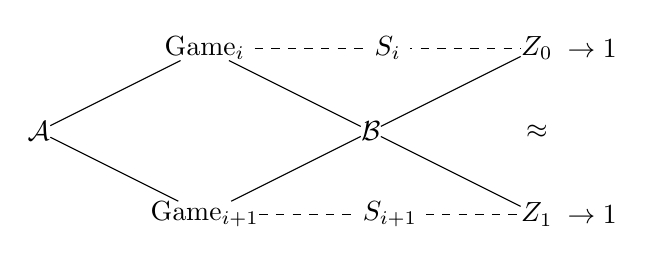
\begin{tikzpicture}
    \node[textnode, name=D] {$\mathcal{B}$}; 
    \node[textnode, right of = D, xshift=6em] {$\approx$}; 
    \node[textnode, name=Z1, right of = D, xshift=6em, yshift=3em] {$Z_0$}; 
    \node[textnode, right of = Z1, xshift=2em] {$\rightarrow 1$}; 
    \node[textnode, name=Z2, right of = D, xshift=6em, yshift=-3em] {$Z_1$};
    \node[textnode, right of = Z2, xshift=2em] {$\rightarrow 1$}; 
    \node[textnode, name=G1, left of = D, xshift=-6em, yshift=3em] {~$\text{Game}_i$~}; 
    \node[textnode, name=G2, left of = D, xshift=-6em, yshift=-3em] {$\text{Game}_{i+1}$};
    \node[textnode, name=A, right of = D, xshift=-12em] {$\mathcal{A}$}; 
    \draw (D) edge[-] (Z1); 
    \draw (D) edge[-] (Z2); 
    \draw (D) edge[-] (G1); 
    \draw (D) edge[-] (G2); 
    \draw (A) edge[-] (G1); 
    \draw (A) edge[-] (G2); 
    \draw (G1) edge[-, dashed] node[midway, fill=white]{$S_i$} (Z1);
    \draw (G2) edge[-, dashed] node[midway, fill=white]{$S_{i+1}$} (Z2); 
\end{tikzpicture}
\end{center}
\caption{基于分布不可区分的游戏演变}\label{figure:IND-change}
\end{figure}
\end{trivlist}

\begin{remark}
许多学术论文在证明的过程中为了简便往往先证明敌手在两个相邻游戏中的视图不可区分, 
再据此得出敌手优势函数的差是可忽略这一结论. 
在多数情形, 这种论证并无问题, 但需要特别小心的是在视图计算不可区分时, 必须同时确保归约算法能够准确判定敌手成功事件才能够确保证明严谨. 
在有些特殊情形, 归约算法无法有效判定敌手是否在游戏中成功, 此时归约算法无法利用敌手成功概率差异打破底层区分性假设, 从而导致归约失效. 
请读者参考文献~\cite{HLL-ASIACRYPT-2016}加深对该证明技术细节的理解和掌握. 
\end{remark}


第二类差异取决于某个特定事件是否发生, 即定义在同一概率空间的两个相邻游戏$\text{Game}_i$和$\text{Game}_{i+1}$仅在某特定事件$F$发生时存在差异, 
在$F$不发生时完全一致, 概率描述如下:  
\begin{equation*}
    S_i \wedge \neg F = S_{i+1} \wedge \neg F
\end{equation*}

为了分析敌手在相邻游戏$\text{Game}_i$和$\text{Game}_{i+1}$中的优势函数差, 需要以下的``差异引理''(difference lemma): 
\begin{lemma}[Difference Lemma]
令$A$, $B$, $F$是定义在同一概率空间中的事件, 
如果$A \wedge \neg F = B \wedge \neg F$, 那么则有$|\Pr[A] - \Pr[B]| \leq \Pr[F]$. 
\end{lemma}
\begin{proof}
差异引理的证明如下, 仅需使用古典概率中简单的缩放技巧: 
\begin{align*}
|\Pr[A] - \Pr[B]| &= |\Pr[A \wedge F]+\Pr[A \wedge \neg F] - \Pr[B \wedge F] - \Pr[B \wedge \neg F]| \blue{//\text{全概率展开}}\\ 
                  &= |\Pr[A \wedge F] - \Pr[B \wedge F]| \blue{//\text{化简}}\\
                  &\leq \max\{\Pr[A \wedge F], \Pr[B \wedge F]\} \leq \Pr[F] \blue{//\text{缩放}}
\end{align*}
证毕! \qed
\end{proof}

根据差异引理, 若需证明$|\Pr[S_i] - \Pr[S_{i+1}]| \leq \mathsf{negl}(\kappa)$, 仅需证明$\Pr[F] \leq \mathsf{negl}(\kappa)$, 
证明细分为以下两种情形:
\begin{itemize}
    \item $F$发生的概率取决于敌手的计算能力, 如敌手找到哈希函数的碰撞或者成功伪造消息认证码. 
        该情形需要建立安全归约, 即若$F$发生, 则存在敌手打破困难问题$X_i$. 
    \item $F$发生的概率与敌手的计算能力无关. 该情形仅需纯粹的信息论论证(information-theoretic argument).
\end{itemize}


第三类差异称为桥接差异. 在分析游戏序列之间的差异时, 有时需要引入桥接步骤对某个变量的生成方式以等价的方式重新定义, 以确保差异分析的良定义.  
桥接步骤引入的差异仅是挑战者侧的概念性变化, 敌手侧的视图完全相同, 因此$\Pr[S_i] = \Pr[S_{i+1}]$. 
桥接步骤看似可有可无, 实则必要, 若不引入必要的桥接步骤, 则会使得证明跳跃难以理解、游戏序列间的差异无法精确分析. 



\section{困难问题}
密码学中常见的困难问题可大致分为数论类和格类, 其中前者是代数问题, 后者是数的几何问题, 
这也正是格类困难问题具备抗量子攻击的原因之一. 

数论类的假设又可进一步分为整数分解类和离散对数类两个分支. 本章首先介绍常见的数论类假设, 再介绍常见的格类困难问题. 

\subsection{整数分解类假设}
整数分解类假设定义在群$\mathbb{Z}_N^*$上. 其中:
\begin{equation*}
\mathbb{Z}_N^* \define \{b \in \{1, \dots, N_1\} \mid \text{gcd}(b, N)=1\}
\end{equation*}
也即$\mathbb{Z}_N^*$是整数集合$\{1, \dots, N-1\}$中所有与$N$互质元素构成的子集, 
在模乘运算$ab \define [ab \bmod N]$下构成交换群.  

以下令$\mathsf{GenModulus}$是多项式时间算法, 其以安全参数$1^\kappa$为输入, 输出$(N=pq, p, q)$, 
其中$p$和$q$(以压倒性概率)是两个$\kappa$-bit的素数. 

\begin{definition}[整数分解假设]
整数分解问题指分解大整数在平均意义下是困难的. 我们称\emph{整数分解假设}相对于$\mathsf{GenModulus}$成立当且仅当对于任意PPT敌手: 
\begin{equation*}
\Pr[\mathcal{A}(N) = (p', q') \text{~s.t.~} p'q' = N] \leq \mathsf{negl}(\kappa)
\end{equation*} 	
上述概率建立在敌手$\mathcal{A}$和$\mathsf{GenModulus}(1^\kappa) \rightarrow (N, p, q)$的随机带上. 
\end{definition}

尽管整数分解假设历经百年的分析攻击仍然健壮, 但是它并不直接蕴含高效的密码系统. 
这就引发密码科技工作者研究与整数分解问题困难性相关问题的研究. 1978年, Rivest, Shamir和Adleman提出了RSA问题. 

令$\mathsf{GenRSA}$是多项式时间算法, 其以安全参数$1^\kappa$为输入, 
输出两个$\kappa$-bit素数的乘积$N$作为模数, 同时输出正整数$(e, d)$满足$ed = 1 \bmod \phi(N)$. 

\begin{definition}[RSA假设]
RSA问题指在平均意义下求解$\mathbb{Z}_N^*$的$e$次方根是困难的. 
我们称\emph{RSA假设}相对于$\mathsf{GenModulus}$成立当且仅当对于任意PPT敌手:
\begin{equation*}
\Pr[\mathcal{A}(N, e, y) = x \text{~s.t.~} x^e = y \bmod N] \leq \mathsf{negl}(\kappa)
\end{equation*} 	
上述概率建立在敌手$\mathcal{A}$、$\mathsf{GenRSA}(1^\kappa) \rightarrow (N, e, d)$和随机选取$x \in \mathbb{Z}_N^*$随机带上. 
\end{definition}

\begin{remark}
RSA问题刻画的是在不知晓$\phi(N)$的情况下计算$\mathbb{Z}_N^*$中随机元素的$e$次方根是困难的. 
容易看出, 如果敌手能够打破整数分解问题, 则可以通过分解$N$求出$\phi(N)$, 进而通过Fermat小定理计算$e$次方根. 
因此, 整数分解问题难于RSA问题, 整数分解假设弱于RSA假设. 
两个假设是否等价仍然未知. 
\end{remark}

给定群$\mathbb{G}$, 称$y \in \mathbb{G}$是一个二次剩余当且仅当$\exists x \in \mathbb{G}$ s.t. $x^2 = y$. 
$x$成为$y$的平方根. 如果一个元素不是二次剩余则称其为二次非剩余. 
在abelian群中, 二次剩余构成子群.

首先考察群$\mathbb{Z}_p^*$中的二次剩余, 其中$p$是素数. 
定义函数$\mathsf{sq}_p: \mathbb{Z}_p^* \rightarrow \mathbb{Z}_p^*$为$\mathsf{sq}_p(x) \define [x^2 \bmod p]$. 
当$p$是大于2的素数时, $\mathsf{sq}_p$是2-对-1函数, 因此立刻可知$\mathbb{Z}_p^*$中恰好一半元素是二次剩余. 
记模$p$的二次剩余集合为$\mathcal{QR}_p$, 模$p$的二次非剩余集合为$\mathcal{QNR}_p$, 我们有: 
\begin{equation*}
|\mathcal{QR}_p| = |\mathcal{QNR}_p| = \frac{|\mathbb{Z}_p^*|}{2} = \frac{p-1}{2}
\end{equation*}

定义元素$x \in \mathbb{Z}_p^*$模$p$的Jacobi符号如下: 
\begin{displaymath}
\mathcal{J}_p(x) \define
\left\{
\begin{array}{l}
+1  \text{~if~} x \in \mathcal{QR}_p\\
+1 \text{~if~} x \in \mathcal{QNR}_p\\
\end{array}
\right.
\end{displaymath}

再考察群$\mathbb{Z}_N^*$中的二次剩余, 其中$N$是两个互异素数$p$和$q$的乘积. 
由中国剩余定理可知: $\mathbb{Z}_N^* \simeq \mathbb{Z}_p^* \times \mathbb{Z}_q^*$, 
令$y \leftrightarrow (y_p, y_q)$表示上述同构映射给出的分解, 易知$y$是模$N$的二次剩余当且仅当$y_p$和$y_q$分别是模$p$和模$q$的二次剩余. 
定义函数$\mathsf{sq}_N: \mathbb{Z}_N^* \rightarrow \mathbb{Z}_N^*$为$\mathsf{sq}_N(x) \define [x^2 \bmod N]$, 
当$N$为互异素数乘积时, $\mathsf{sq}_N$是4--对--1函数. 
记模$N$的二次剩余集合为$\mathcal{QR}_N$, 由$\mathcal{QR}_N$与$\mathcal{QR}_p \times \mathcal{QR}_q$之间的一一对应关系可知: 

\begin{equation*}
\frac{|\mathcal{QR}_N|}{|\mathbb{Z}_N^*|} = \frac{|\mathcal{QR}_p| \cdot |\mathcal{QR}_q|}{|\mathbb{Z}_N^*|} 
= \frac{1}{4}
\end{equation*}

从二次剩余的角度可以对$\mathbb{Z}_N^*$中的元素进行如下的划分: 
(i) $\mathbb{Z}_N^*$可以划分为相同大小的$\mathcal{J}_N^{+1}$和$\mathcal{J}_N^{-1}$(Jacobi符号分别为1和-1); 
(ii) $\mathcal{J}_N^{+1}$有可以划分为$\mathcal{QR}_N$和$\mathcal{QNR}_N^{+1}$, 
其中$\mathcal{QNR}_N^{+1} \define \{x \in \mathbb{Z}_N^* \mid x \notin \mathcal{QR}_N \wedge \mathcal{J}_N(x)=+1\}$.  

\begin{definition}[模二次剩余假设]
模二次剩余(QR, quadratic residue)假设指$\mathcal{QR}_N$上的均匀分布与$\mathcal{QNR}_N^{+1}$上的均匀分布计算不可区分. 
我们称\emph{模二次剩余假设}相对于$\mathsf{GenModulus}$成立当且仅当对于任意PPT敌手:  
\begin{equation*}
|\Pr[\mathcal{A}(N, y_0) = 1] - \Pr[\mathcal{A}(N, y_1) = 1]| \leq \mathsf{negl}(\kappa)
\end{equation*}		
上述概率建立在敌手$\mathcal{A}$、$\mathsf{GenModulus}(1^\kappa) \rightarrow (N, p, q)$和
随机选取$y_0 \in \mathcal{QR}_N, y_1 \in \mathcal{QNR}_N^{+1}$的随机带上. 
\end{definition}

与QR假设应用紧密相关的技术细节是如何对$\mathcal{QR}_N$和$\mathcal{QNR}_N^{+1}$进行高效的均匀采样. 
\begin{itemize}
\item 对$\mathcal{QR}_N$进行均匀采样较为简单: 仅需随机选取$x \in \mathbb{Z}_N^*$再令$y:= x^2 \bmod N$即可. 
	注意到$x^2 \bmod N$是一个4-to-1的正则函数, 因此当$x \sample \mathbb{Z}_N^*$时, 输出$y$服从$\mathcal{QR}_N$上的均匀分布. 

\item 对$\mathcal{QNR}_N^{+1}$进行均匀采样稍显复杂, 当$N$的分解未知时如何均匀采样未知. 
	我们可以借助辅助信息$z \in \mathcal{QNR}_N^{+1}$完成采样, 即随机选取$x \in \mathbb{Z}_N^*$, 
	输出$y:= z \cdot x^2 \bmod N$. 可以验证, 当$x \sample \mathbb{Z}_N^*$时, 输出$y$服从$\mathcal{QNR}_N^{+1}$上的均匀分布. 
\end{itemize}


\begin{remark}
显然, 整数分解问题难于二次剩余判定问题, 因此整数分解假设弱于模二次剩余判定假设. 
两个假设是否等价仍然未知. 
\end{remark}

\begin{definition}[模平方根假设]
模平方根(SQR, square root)假设指对$\mathcal{QN}_N$中的随机元素求平方根是困难的. 
我们称\emph{模平方根假设}相对于$\mathsf{GenModulus}$成立当且仅当对于任意PPT敌手:  
\begin{equation*}
\Pr[\mathcal{A}(N, y) = x \text{~s.t.~} x^2 = y \bmod N] \leq \mathsf{negl}(\kappa)
\end{equation*}	
上述概率建立在敌手$\mathcal{A}$、$\mathsf{GenModulus}(1^\kappa) \rightarrow (N, p, q)$和
随机选取$y \in \mathcal{QR}_N$的随机带上. 
\end{definition}

令$p$和$q$是两个互异的模4余3的素数, 则称$N = pq$是Blum整数. 我们有以下推论: 
\begin{proposition}
当$N$时Blum整数时, 则每个模$N$的二次剩余有且仅有一个平方根是二次剩余.
\end{proposition}
上述推论保证了当$N$是Blum整数时, 函数$f_N \define [x^2 \bmod N]$构成$\mathcal{QR}_N$上的置换. 这一性质在构造加密方案时至关重要. 

\begin{remark}
模平方根假设等价于整数分解假设, 即在未知$N$分解的情况下求模平方根与分解$N$一样困难.  
\end{remark}

综上, 整数分解类问题的困难性关系如图~\ref{figure:factoring-type-problems-relation}所示: 
\begin{figure}[!hbtp]
\begin{center}
\begin{tikzpicture}
\node[textnode, name=factoring] {整数分解问题}; 
\node[textnode, right of = factoring, xshift=5em] {$\equiv$}; 
\node[textnode, name=SQR, right of = factoring, xshift=10em] {求模平方根问题}; 
\node[textnode, name=RSA, right of = SQR, anchor=west, xshift=8em, yshift=4em] {$\succeq$RSA问题};
\node[textnode, name=QR, right of = SQR, anchor=west, xshift=8em, yshift=-4em] {$\succeq$模二次剩余问题}; 
\draw (SQR.east) edge[-] (RSA.west); 
\draw (SQR.east) edge[-] (QR.west); 
\end{tikzpicture}
\end{center}
\caption{整数分解类问题的困难性关系}\label{figure:factoring-type-problems-relation}
\end{figure}

\subsection{离散对数类假设}
离散对数类假设定义在循环群$\mathbb{G}$中. 
令$\mathsf{GenGroup}$是多项式时间算法, 其以安全参数$1^\kappa$为输入, 输出$q$阶循环群$\mathbb{G} = \langle g \rangle$的描述, 
其中, $q$是$\kappa$-bit的整数, 简记为$(\mathbb{G}, q, g) \leftarrow \mathsf{GenGroup}(1^\kappa)$. 
为了行文方便, 本书中假设$\mathbb{G}$为加法群, 用``$\cdot$''表示群运算.  
由循环群的定义可知, $\mathbb{G}$中的元素为$\{g^0, g^1, \dots, g^{q-1}\}$. 因此, 对于任意$h \in \mathbb{G}$
存在唯一的$x \in \mathbb{Z}_q$使得$g^x = h$, 我们称$x$是$h$相对于生成元$g$的离散对数并记为$x = \log_g h$, 
这里称其为离散对数强调其取值均为非负整数, 有别于标准算术对数的取值为实数.  



\begin{definition}[离散对数假设]
离散对数问题指在平均意义下求解群元素的离散对数是困难的. 
我们称\emph{离散对数(DLOG)假设}相对于$\mathsf{GenGroup}$成立当且仅当对于任意PPT敌手: 
\begin{equation*}
\Pr[\mathcal{A}(\mathbb{G}, q, g, h) = \log_g h] \leq \mathsf{negl}(\kappa)
\end{equation*} 
上述概率建立在敌手$\mathcal{A}$、$\mathsf{GenGroup}(1^\kappa) \rightarrow (\mathbb{G}, q, g)$和随机采样$h \in \mathbb{G}$的随机带上. 
\end{definition}

显然, 离散对数假设说明了$x \mapsto g^x$是从$\mathbb{Z}_q$到$\mathbb{G}$的单向函数. 
单向函数能够蕴含的密码方案有限, 下面介绍与离散对数假设相关的其它假设, 它们能够作为更多密码方案的安全基础. 
这类困难假设的起源于Diffie和Hellman~\cite{DH-IEEE-IT-1976}在1976年的划时代论文, 
后来被称为Diffie-Hellman假设. 
为了叙述方便, 我们首先定义DH函数$\mathsf{DH}_g: \mathbb{G}^2 \rightarrow \mathbb{G}$, 
\begin{equation*}
\mathsf{DH}_g(h_1, h_2) \define g^{\log_g h_1 \cdot \log_g h_2}
\end{equation*} 

% \begin{equation*}
% (g^a)^b = g^{ab} = (g^b)^a
% \end{equation*}

% \begin{equation*}
% g^{\red{x}} = y
% \end{equation*}

% \begin{equation*}
% \red{m}^e = c
% \end{equation*}

Diffie-Hellman类假设可细分为两类, 一类是计算性Diffie-Hellman (CDH)问题, 一类是判定性Diffie-Hellman (DDH)问题. 
下面依次介绍.

\begin{definition}[CDH假设]
CDH问题指在平均意义下计算$\mathsf{DH}_g$函数是困难的. 
我们称\emph{CDH假设}相对于$\mathsf{GenGroup}$成立当且仅当对于任意PPT敌手: 
\begin{equation*}
\Pr[\mathcal{A}(\mathbb{G}, q, g, g^a, g^b) = g^c] \leq \mathsf{negl}(\kappa)
\end{equation*} 	
上述概率建立在敌手$\mathcal{A}$、$\mathsf{GenGroup}(1^\kappa) \rightarrow (\mathbb{G}, q, g)$和随机采样$a, b \in \mathbb{Z}_q$的随机带上. 
\end{definition}  

\begin{definition}[DDH假设]
对于四元组$(g, g^a, g^b, g^c)$, 如果$g^c = \mathsf{DH}_g(g^a, g^b)$也即$ab = c \bmod q$, 则称其为DH元组. 
DDH假设刻画的是随机DH元组和随机四元组是计算不可区分的. 我们称\emph{DDH假设}相对于$\mathsf{GenGroup}$成立当且仅当对于任意PPT敌手: 
\begin{equation*}
|\Pr[\mathcal{A}(\mathbb{G}, q, g, g^a, g^b, g^{ab})=1] - \Pr[\mathcal{A}(\mathbb{G}, q, g, g^a, g^b, g^c)=1]| 
\leq \mathsf{negl}(\kappa)
\end{equation*}  
上述概率建立在敌手$\mathcal{A}$、$\mathsf{GenGroup}(1^\kappa) \rightarrow (\mathbb{G}, q, g)$和随机采样$a, b, c \in \mathbb{Z}_q$的随机带上. 
\end{definition} 

离散对数类问题的困难性关系如图~\ref{figure:dlog-type-problems-relation}所示: 
\begin{figure}[!hbtp]
\begin{center}
\begin{tikzpicture}
\node[textnode, name=dlog] {离散对数问题}; 
\node[textnode, right of = dlog, xshift=5em] {$\succeq$}; 
\node[textnode, name=CDH, right of = dlog, xshift=10em] {CDH问题}; 
\node[textnode, right of = CDH, xshift=5em] {$\succeq$}; 
\node[textnode, name=DDH, right of = CDH, xshift=10em] {DDH问题}; 
\end{tikzpicture}
\end{center}
\caption{离散对数类问题的困难性关系}\label{figure:dlog-type-problems-relation}
\end{figure}

\begin{remark}
注意到任何$q$阶循环群均与$\mathbb{Z}_q$是同构的, 而$\mathbb{Z}_q$上的离散对数问题时容易的. 
因此在实例化循环群$\mathbb{G}$必须谨慎审慎, 这也从一个方面说明离散对数类问题的困难性与底层代数结构的具体特性(如群的表示)紧密相关. 
对于$\mathbb{G}$的实例化, 通常既可以选择$\mathbb{F}_{p^k}^*$的素数阶乘法子群, 
也可以选择椭圆曲线上的素数阶乘法群. 
另外强调一点, 存在这样的循环群$\mathbb{G}$(如双线性映射群)使得离散对数、CDH假设成立, 而DDH假设不成立. 
\end{remark}


\subsection{格类假设} 
1997年, Shor~\cite{Shor-SIAM-1997}给出了数论类问题(包括整数分解类和离散对数类)的有效量子算法. 
在未来, 如果大规模量子计算机研制成功, 则数论类假设将不再成立. 迄今为止, 尚未有针对格基困难问题的有效量子算法, 
通用的量子算法仅相对非量子算法有些许优势. 目前普遍的共识是格基困难问题具备抗量子安全能力, 这正是该类问题倍受关注的主要原因. 

本小节中将介绍两个主要的平均意义下的格基困难问题, 短整数解问题和带误差学习问题. 
需要提前说明的是, 格基困难问题的困难性与参数的选取密切相关, 因此格基问题的描述相比数论类问题要复杂得多. 

Ajtai~\cite{Ajtai-STOC-1996}在1996年的开创性论文中正式提出了短整数解(short integer solution, SIS)问题. 
SIS问题不仅可以作为所有Minicrypt世界中密码组件的安全基础, 包括单向函数、身份鉴别协议、数字签名, 
还可以用来构造抗碰撞哈希函数. 非正式的, SIS问题指在给定许多较大的有限加法群中随机选取的元素, 找到足够``短''的整系数组合使得其和是0是困难的. 
SIS问题由以下参数刻画:    
\begin{itemize}
	\item 正整数$n$和$q$, 用于刻画加法群$\mathbb{Z}_q^n$; 
	\item 正实数$\beta$, 用于刻画解向量的长度; 
	\item 正整数$m$, 用于表征群元素的个数. 
\end{itemize}
其中$n$是主要的参数(如: $n \geq 100$), $q > \beta$通常设定为关于$n$的小多项式. 

\begin{definition}[短整数解假设($\text{SIS}_{n, q, \beta, m}$)]
我们称\emph{SIS假设}成立当且仅当对于任意PPT敌手:
\begin{equation*}
\Pr[\mathcal{A}(\mathbf{a}_1, \dots, \mathbf{a}_m) = \mathbf{z} \neq \mathbf{0} \in \mathbb{Z}^m \text{~s.t.~} 
\sum_{i}^m \mathbf{a}_i z_i = \mathbf{0} \in \mathbb{Z}_q^n \wedge \lVert z \rVert \leq \beta] \leq \mathsf{negl}(\kappa) 
\end{equation*} 
上述概率建立在敌手$\mathcal{A}$和随机选取$\mathbf{a}_i \in \mathbb{Z}^m$的随机带上. 
\end{definition}
以上定义中$m$个$\mathbb{Z}_q^n$上的随机向量可以按列向量的方式组成矩阵$\mathbf{A} \in \mathbb{Z}_q^{n \times m}$. 
因此, SIS假设实质上在要求找到函数$f_\mathbf{A}(\mathbf{z}) := \mathbf{A} \mathbf{z}$的短整数非零向量原像是困难的. 

下面简单讨论参数选取与问题困难性之间的关联: 
\begin{itemize}
\item 如果不对$\lVert z \rVert$进行限制, 那么可以轻易利用Gaussian消元法找到一个整数解. 
	同时, 我们必须要求$\beta < q$, 否则$\mathbf{z} = (q, 0, \dots, 0) \in \mathbb{Z}^m$即构成一个合法的非平凡解. 

\item 注意到任何关于矩阵$\mathbf{A}$的短整数解可通过补$0$平凡地延展为关于矩阵$[\mathbf{A} \mid \mathbf{A}']$的解. 
	换言之, SIS问题的困难性随着$m$的增大变得容易. 对应的, SIS问题的困难性随着$n$增加变得困难. 

\item 向量范数界$\beta$和向量$\mathbf{a}_i$的个数$m$必须足够大以保证解的存在性. 
	令$\bar{m}$是大于$n \log q$的最小正整数, 则我们必须有$\beta > \sqrt{\bar{m}}$和$m \geq \bar{m}$. 
	不失一般性, 不妨假设$m = \bar{m}$, 则存在超过$q^n$个向量$\mathbf{x} \in \{0,1\}^m$, 
	根据鸽巢原理, 则必有$\mathbf{x} \neq \mathbf{x}'$使得$\mathbf{A}\mathbf{x} = \mathbf{A}\mathbf{x}' \in \mathbb{Z}_q^n$, 
	从而它们的差值$\mathbf{z} = \mathbf{x} - \mathbf{x}' \in \{0, \pm 1\}^m$是范数小于$\beta$的短整数解. 

\item 上述的鸽巢原理论证事实上蕴含更多深意: 函数族$\{f_\mathbf{A}: \{0,1\}^m \rightarrow \mathbb{Z}_q^n\}$基于SIS假设是抗碰撞的. 
	若不然, 给定关于$f_\mathbf{A}$的一对碰撞$\mathbf{x}, \mathbf{x}' \in \{0,1\}^m$, 则立刻诱导出关于$\mathbf{A}$的一个短整数解. 
\end{itemize}

SIS问题可以被理解为在以下特定$q$元$m$维整数格中的平均意义短向量问题(short-vector problem, SVP), 该整数格的定义为: 
\begin{equation*}
\mathcal{L}^{\bot}(\mathbf{A}) \define \{\mathbf{z} \in \mathbb{Z}^m: \mathbf{A}\mathbf{z} = 0 \in \mathbb{Z}_q^n\} 
\supseteq q\mathbb{Z}^m
\end{equation*}
从编码的角度理解, $\mathbb{A}$扮演着格/码字$\mathcal{L}^{\bot}(\mathbf{A})$校验矩阵的角色. 
SIS问题的困难性指对于随机选取的$\mathbf{A}$, 找到一个短的码字是困难的. 


Regev~\cite{Regev-STOC-2005}在2005年的开创性论文中提出了另一个平均意义下的重要格基困难问题--带误差学习问题(learning with errors, LWE). 
LWE问题与SIS问题互相对偶, 能够蕴含Minicrypt之外的密码体制. 

在正式定义LWE问题之前, 首先引入LWE分布的概念. 称向量$\mathbf{s} \in \mathbb{Z}_q^n$为秘密, 
LWE分布$A_{\mathbf{s}, \chi}$定义在$\mathbb{Z}_q^n \times \mathbb{Z}_q$上, 
采样算法为随机选取$\mathbf{a} \in \mathbb{Z}_q^n$, 选取$e \leftarrow \chi$, 
输出$(\mathbf{a}, b = \langle \mathbf{s}, \mathbf{a}\rangle+e \bmod q)$. 

LWE问题有两个版本, 其中搜索版本要求给定LWE采样求解秘密, 判定版本要求区分LWE采样和随机采样. 
LWE问题由以下参数刻画: 
\begin{itemize}
\item 正整数$n$和$q$, 和SIS问题一样, 用于刻画加法群$\mathbb{Z}_q^n$;
\item 正整数$m$表征采样的个数, 通常选取的足够大以保证秘密的惟一性; 
\item $\mathbb{Z}$上的误差分布$\chi$, 通常的选取是宽度为$\alpha q$的离散Gaussian分布, 其中$\alpha < 1$称为相对错误率. 
\end{itemize} 

\begin{definition}[搜索LWE假设]
搜索LWE问题指给定$m$个$A_{\mathbf{s}, \chi}$的独立随机采样, 求解秘密向量$\mathbf{s}$是困难的. 
我们称\emph{搜索LWE假设}成立当且仅当对于任意PPT敌手:
\begin{equation*}
\Pr[\mathcal{A}(\{\mathbf{a}_i, b\}_{i=1}^m \leftarrow A_{\mathbf{s}, \chi}) = \mathbf{s}] \leq \mathsf{negl}(\kappa) 
\end{equation*} 
上述概率建立在敌手$\mathcal{A}$、随机选取$\mathbf{s} \in \mathbb{Z}_q^n$和采样$A_{\mathbf{s}, \chi}$的随机带上. 
\end{definition}

\begin{definition}[判定LWE假设]
判定LWE问题指区分$m$个独立采样是来自$A_{\mathbf{s}, \chi}$分布还是随机分布是困难的. 
我们称\emph{判定LWE假设}成立当且仅当对于任意PPT敌手:
\begin{equation*}
|\Pr[\mathcal{A}(\{\mathbf{a}_i, b\}_{i=1}^m \leftarrow A_{\mathbf{s}, \chi}) = 1] - 
 \Pr[\mathcal{A}(\{\mathbf{a}_i, b\}_{i=1}^m \leftarrow U_{\mathbb{Z}_q^n \times \mathbb{Z}_q}) = 1] \leq \mathsf{negl}(\kappa) 
\end{equation*} 
上述概率建立在敌手$\mathcal{A}$、随机选取$\mathbf{s} \in \mathbb{Z}_q^n$和采样$A_{\mathbf{s}, \chi}$
以及$U_{\mathbb{Z}_q^n \times \mathbb{Z}_q}$的随机带上. 
\end{definition}

\begin{remark}
LWE问题时LPN问题(learning parities with noise)的一般化. 在LPN问题中, $q=2$, $\chi$为$\{0,1\}$上的Bernoulli分布. 
\end{remark}

下面简单讨论参数选取与问题困难性之间的关联: 
\begin{itemize}
\item 如果没有误差分布$\chi$, 则LWE问题的搜索版本和判定版本均可利用Gaussian消元法快速求解. 

\item 和SIS问题类似, 可以用矩阵的语言更简洁的描述LWE问题: 
	(i) 将$m$个向量$\mathbf{a}_i \in \mathbb{Z}_q^n$汇聚为矩阵$\mathbf{A} \in \mathbb{Z}_q^{n \times m}$; 
	(ii) 将$m$个$b_i \in \mathbb{Z}_q$汇聚为向量$\mathbf{b} \in \mathbb{Z}_q^n$, 因此对于LWE采样我们有: 
	\begin{equation*}
		\mathbf{b}^t = \mathbf{s}^t \mathbf{A} + \mathbf{e}^t (\bmod q),
	\end{equation*}
	其中$\mathbf{e} \leftarrow \chi^m$. 
\end{itemize}

LWE问题可以被理解为在以下特定$q$元$m$维整数格中的平均意义有界距离解码问题(bounded-distance decoding problem, BDD), 该整数格的定义为: 
\begin{equation*}
\mathcal{L}(\mathbf{A}) \define \{\mathbf{A}^t \mathbf{s}: \mathbf{s} \in \mathbb{Z}_q^n\}+q \mathbb{Z}^m 
\end{equation*}

从编码的角度理解, $\mathbf{A}$扮演着格/码字$\mathcal{L}(\mathbf{A})$生成矩阵的角色. 
对于LWE采样, $\mathbf{b}$与格中的惟一向量/码字相近, 搜索版本要求计算秘密向量$s$, 即根据带误差的码字进行解码. 
对于随机采样, $\mathbf{b}$以大概率远离格$\mathcal{L}(\mathbf{A})$中所有向量.   
SIS问题的困难性指对于随机选取的$\mathbf{A}$, 找到一个短的码字是困难的. 
\section{复杂性理论初步}
在复杂性理论中, 困难问$P$通常定义在$L \subseteq X$上, $X$是所有实例的集合, $L$是$X$中满足特定性质的一个子集. 
我们称$P$是可高效判定/求解的, 如果存在确定性时间的Turing机$M$满足: 
\begin{equation*}
	x \in L \iff M(x) = 1  
\end{equation*}
所有可高效判定/求解问题的合集组成$\mathcal{P}$复杂性类. 

\begin{note}
实例集合$X$的学术术语是词(words), 子集$L$对应的学术术语是语言(language). 
术语的来源是一个自然的类比: 不妨设世界上所有的词汇构成一个集合, 那么汉语、英语、法语、德语、C++语言、Rust语言等多种多样的语言自然构成了这个集合的各个子集.  
通常, 称语言内的元素为Yes实例, 语言外的元素为No实例. 
\end{note}

密码学中的困难问题可以分为计算和判定两类: 
\begin{itemize}
	\item 计算类(也称搜索类)问题要求计算出问题的解: 如RSA问题、离散对数问题、计算Diffie-Hellman问题、短整数解问题等. 
	\item 判定类问题要求判定是或否: 如二次剩余问题、判定Diffie-Hellman问题、判定LWE问题等. 
\end{itemize}
从解空间的角度理解, 判定问题可以看做计算问题的特例, 即输出解为1比特. 通常, 同一个问题的计算版本难于判定版本, 对应的计算假设弱于判定假设.    

困难的二元关系是对密码学中各种计算类困难问题的抽象.  
\begin{definition}[二元关系(binary relation)]
令$L \subseteq X$是一个$\mathcal{NP}$语言. 
$L$由二元关系$\mathsf{R}_L: X \times W$定义, 其中$W$之证据集合: 
\begin{equation*}
    x \in L \Leftrightarrow \exists w \in W \text{~s.t.~} (x, w) \in \mathsf{R}_L
\end{equation*}

如果$\mathsf{R}_L$满足如下两个性质, 则称其是困难的(hard):
\begin{itemize}
    \item 易采样 (easy to sample):  $\exists$ PPT算法$\mathsf{SampR}$对关系$\mathsf{R}_L$进行随机采样, 
    	其以公开参数$pp$为输入, 输出``实例-证据''元组$(x, w) \in \mathsf{R}_L$. 

    \item 难抽取 (hard to extract): $\forall$ PPT敌手$\mathcal{A}$:
    \begin{equation*} 
    	\Pr[(x, \mathcal{A}(x) = w') \in \mathsf{R}_L: (x, w) \leftarrow \mathsf{SampR}(pp)] \leq \mathsf{negl}(\kappa)
    \end{equation*}
\end{itemize} 
\end{definition}

\begin{note}
单向函数自然诱导了一个困难的二元关系. 
易采样的性质由单向函数的定义域可高效采样和单向函数可高效求值两点保证, 难抽取的性质由单向函数的单向性保证.
\end{note}

\begin{figure}[!htbp]
\begin{center}
\begin{tikzpicture}
    \node [name = X, circlenode, fill=gray!40, minimum size=5.5em, label={[xshift=0em, yshift=-1.5em]$X$}] {}; 
    \node [name = L, circlenode, fill=violet!70, minimum size=2em, inner sep = 0em] {$L$};
    \node [name = W, circlenode, fill=cyan, right of = L, xshift = 10em, minimum size=2em, inner sep=0em] {$W$}; 
    \node [name = SampR, textnode, right of = X, xshift = 5em, yshift=-2.5em] {$\mathsf{SampR}(pp)$}; 

    \node [textnode, above of = L, yshift=5em, xshift=5em] 
        {\red{问题任务:} 计算/搜索 \quad \quad \mdblue{解空间:} $\{0,1\}^{\mathsf{poly}(\kappa)}$};  

    \draw (L) edge[<->] node[above] {$\mathsf{R}_L$} (W); 
    \draw (SampR) edge[->] (L); 
    \draw (SampR) edge[->] (W);
\end{tikzpicture}
\end{center}
\caption{计算类困难问题图示}
\end{figure}
 
% \begin{block}{Computation Assumption $\Leftarrow$ Hard Relation}
% \begin{itemize}
%     \item problem --- instance 
%     \item solution --- witness 
%     \item Given $x \sample L$, it is hard to find $w$ s.t. $(x, w) \in \mathsf{R}_L$. 
% \end{itemize}
% \end{block}



子集成员判定问题(SMP, Subset Membership Problem)则是密码学中各种判定类问题的抽象. 

\begin{definition}[子集成员判定问题]
令$L \subset X$是一个语言, 公开参数是$pp$. 定义以3个PPT采样算法:
\begin{itemize}
	\item $\mathsf{SampAll}(pp)$: 输出$X$中的随机元素. 
	\item $\mathsf{SampYes}(pp)$: 输出$L$中的随机元素, 即随机Yes实例. 
	\item $\mathsf{SampNo}(pp)$: 输出$X \backslash L$中的随机元素, 即随机No实例. 
\end{itemize} 

SMP问题有两种类型: 
\begin{itemize}
    \item Type 1: $U_X \approx_c U_L$
    \item Type 2: $U_{X \backslash L} \approx_c U_L$
\end{itemize}
\end{definition}

\begin{remark}
定义$\rho = |L|/|X|$为语言$L$相对于$X$的密度. 容易证明: 
\begin{itemize}
    \item 当$\rho = \mathsf{negl}(\kappa)$时: Type 1 $\iff$ Type 2
    \item 当$\rho$已知时: Type 2 $\Rightarrow$ Type 1 
    \begin{itemize}
    	\item 归约的方法是对给定分布和$U_L$分布根据$\rho$进行加权重构: 
    		如果给定分布是$U_{X \backslash L}$, 则重构结果$U_X$; 如果给定分布是$U_L$, 则重构结果仍为$U_L$. 
    		因此, Type 2的实例可以归约到Type 1的实例. 
    \end{itemize}
\end{itemize}
\end{remark}

\begin{figure}[!htbp]
\begin{center}
\begin{tikzpicture}
    \node [name = X, circlenode, fill=gray!40, minimum size=5.5em, label={[xshift=0em, yshift=-1.5em]$X$}] {}; 
    \node [name = L, circlenode, fill=violet!70, minimum size=2em, inner sep = 0em] {$L$};
    \node [name = SampAll, textnode, left of = X, xshift=-7em, yshift=2.5em] {$\mathsf{SampAll}(pp)$};
    \node [name = SampYes, textnode, left of = X, xshift=-7em, yshift=0em] {$\mathsf{SampYes}(pp)$}; 
    \node [name = SampNo, textnode, left of = X, xshift=-7em, yshift=-2.5em] {$\mathsf{SampNo}(pp)$}; 

    \node [textnode, above of = X, yshift=5em, xshift=3em] 
        {\red{问题任务:} 区分/判定 \quad \quad \mdblue{解空间:} $\{0,1\}$};  

    \draw (SampAll) edge[->] (X); 
    \draw (SampYes) edge[->] (L); 
    \draw (SampNo) edge[->] ($(L.south)+(-1em, -0.2em)$); 
\end{tikzpicture}
\end{center}
\caption{判定类计算问题示例}
\end{figure}
 




\section{信息论工具}
\subsection{熵的概念}
Shannon在1948年开创了信息论这一全新领域, 其工作的开创性不啻于Einstein关于引力场理论的工作, 
一举奠定了学科的基础, 解答了最初所有最重要的问题.  
 
Shannon的信息论关注的重点是``消息''和它们在(有噪)信道中的传播. 
容易直观理解的是, 消息所包含的信息量取决于消息令人感到意外的程度(如果消息平平无奇, 那么它包含的信息为0). 
相比而言, 稍显反直觉的是随机消息包含最多的信息. 

信息论中最重要的概念是熵(entropy). 熵量化了期望的意义下消息包含的信息量, 单位通常是比特.    
从概率论的角度看, 熵是对随机变量不确定性的测度.  
以下令令$X$是定义在$\Omega$上的随机变量.
\begin{definition}[熵]
$X$的熵刻画了平均意义下$X$取值的(不)可预测性: 
\begin{equation*}
    \entropy(X) = - \sum_{\omega \in \Omega} \Pr[X = \omega] \log \Pr[X = \omega]
\end{equation*} 
\end{definition} 

\begin{remark}
一个消息的熵就是消息所包含信息的比特数, 用编码的语言刻画, 就是编码该消息所需的最短比特数.
\end{remark}

密码方案/协议的安全性分析均是针对恶意敌手展开的. 
敌手单次正确预测某随机变量(如私钥)值的概率与密码方案/协议的安全性紧密相关. 显然, 敌手的最佳策略是猜测最大似然值. 
在本章中, 我们用大写字母$X$表示随机变量, 用小写字母$x$表示$X$的取值, 用花体字母$\mathcal{X}$表示$X$的支撑集. 

一个随机变量$X$的最大可预测性是$\max_{\omega \in \Omega} \Pr[X = \omega]$. 
最大可预测性对应最小熵(min-entropy), 严格定义如下:  
\begin{definition}[最小熵]
$X$的最小熵刻画了$X$的最大可预测性: 
\begin{equation*}
    \minentropy(X) = - \log \left(\max_{\omega \in \Omega} \Pr[X = \omega]\right)
\end{equation*} 
\end{definition} 
\begin{remark}
最小熵可以看做``最坏情形''(worst-case)的熵.
\end{remark}

在很多场景中, 随机变量$X$与另一随机变量$Y$相关, 并且敌手知晓$Y$的取值.  
因此, Dodis等~\cite{DORS-SIAM-2008}引入了平均最小熵(average min-entropy)来刻画$X|Y$的(不)可预测性:
\begin{equation}\label{equation:average-min-entropy}  
    \avminentropy(X|Y) = - \log\left(\mathbb{E}_{y \leftarrow Y} \left[2^{−\minentropy(X|Y =y)}\right]\right)
                       = - \log\left(\mathbb{E}_{y \leftarrow Y} \left[\max_{\omega \in \Omega}\Pr[X=\omega|Y =y]\right]\right)
\end{equation}

以下浅释平均最小熵的定义直觉. 考虑一对变量$X$和$Y$(两者可能相关). 
如果敌手知晓$Y$的取值$y$, 则$X$在敌手视角中的可预测性是$\max_{x} \Pr[X = x|Y = y]$. 
在平均的意义下(对$Y$做期望), 敌手成功预测$X$的概率为 
$\mathbb{E}_{y \leftarrow Y}[\max_x \Pr[X = x|Y = y]]$. 

平均最小熵的定义在对$Y$做加权平均的前提下($Y$的取值不受敌手控制)测度$X$最坏情形下的可预测性
(敌手知晓$y$后对$X$的预测是恶意行为). 一个微妙的细节是平均最小熵的定义~\eqref{equation:average-min-entropy}
先对预测成功的概率做期望后再取对数, 
那能否交换$\log$和$\expect$的次序呢? 定义平均最小熵$\expect_{y \leftarrow Y}[\minentropy(X|Y = y)]$是否合理呢?
交换次序后的定义失去了原本的意义. 
考虑以下的例子, 令$X$和$Y$都是定义在$\Omega = \{0,1\}^{1000}$上的随机变量, 
$Y$是$\Omega$上的随机分布, 当$Y$的取值$y$的首bit为0时, $X$的取值与$y$相同, 否则随机分布. 
因此对于$Y$的半数取值$y$, $\minentropy(X | Y = y) = 0$, 对另外半数取值, $\minentropy(X|Y=y)=1000$, 
所以$\expect_{y \leftarrow Y}[\minentropy(X|Y=y)]=500$. 
然而, 声称$X$具有500比特的安全性显然不符合逻辑. 
事实上, 知晓$Y$取值$y$的敌手直接输出$y$, 既能够以大于$1/2$的概率猜对$X$的取值. 
平均最小熵标准的定义准确刻画了至少$1/2$得可预测性, 因为$\avminentropy(X|Y)$略小于1.
我们也可以从数学的角度解释如下, $\expect$是线性算子, 而$\log$是非线性算子, 因此次序交换后意义不同.  

平均最小熵和最小熵之间存在何种关系呢? 
Dodis等~\cite{DORS-SIAM-2008}证明了如下的cChainning Lemma, 建立了两者之间的关系, 给出了平均最小熵的一个下界. 
\begin{lemma}[Chainning Lemma]\label{lemma:chainning-lemma}
令$X$、$Y$和$Z$是三个随机变量(可任意相关), 其中$Y$的支撑集包含至多$2^r$个元素. 
我们有$\avminentropy(X|(Y,Z)) \geq \minentropy(X|Z) - r$. 
特别的, 当$Z$为空时, 上述不等式简化为: $\avminentropy(X|Y) \geq \minentropy(X) - r$. 
\end{lemma}

\subsection{随机性提取}
随机性是密码学的主旋律, 几乎所有已知密码方案/协议都离不开均匀随机采样. 
然而, 均匀无偏的完美信源并不易得, 很多场景下存在的是有偏的弱信源. 如何在信源有偏的情况下进行均匀随机采样呢? 这就是随机性提取器所要完成的工作. 

\begin{definition}[强随机性提取器]
令$X$是最小熵$\minentropy(X) \geq n$的随机变量,  
$\mathsf{ext}: \mathcal{X} \times \mathcal{S} \rightarrow \mathcal{Y}$是一个可高效计算的函数. 
我们称$\mathsf{ext}$是对信源$X$的$(n, \epsilon)$-强随机性提取器当且仅当以下成立:
\begin{equation*}
    \Delta((\mathsf{ext}(X, S), S), (Y, S)) \leq \epsilon,
\end{equation*} 
其中$S$是定义在$\mathcal{S}$上的均匀随机变量, $Y$是定义在$\mathcal{Y}$上的均匀随机变量. 
\end{definition}

类比于平均最小熵和最小熵之间的关系, 当信源$X$与另一变量$Z$相关时, 我们需要引入平均强随机性提取器来对信源$X$进行萃取.  
\begin{definition}[平均强随机性提取器]
令$(X, Z)$是满足约束$\avminentropy(X|Z) \geq n$的任意变量对, 
$\mathsf{ext}: \mathcal{X} \times \mathcal{S} \rightarrow \mathcal{Y}$是一个可高效计算的函数. 
我们称$\mathsf{ext}$是对信源$X$的平均意义$(n, \epsilon)$-强随机性提取器当且仅当以下成立:
\begin{equation*}
    \Delta((\mathsf{ext}(X, S), S, Z), (Y, S, Z)) \leq \epsilon,
\end{equation*} 
其中$S$是定义在$\mathcal{S}$上的均匀随机变量, $Y$是定义在$\mathcal{Y}$上的均匀随机变量. 
\end{definition}

Dodis等~\cite{DORS-SIAM-2008}的Leftover Hash Lemma(剩余哈希引理)证明了任何强随机性提取性在适当的参数设定下都是平均强随机性提取器. 
作为一个特例, Dodis等证明了任何一族一致哈希函数(universal hash functions)都是平均强随机性提取器.

\begin{lemma}[Leftover Hash Lemma]\label{lemma:leftover-hash-lemma} 
令$X$和$Z$是满足约束$\avminentropy(X|Z) \geq n$的任意变量对, 
$\mathcal{H} = \{h_s: \mathcal{X} \rightarrow \mathcal{Y}\}_{s \leftarrow S}$是一族一致哈希函数. 
那么当$n \geq \log |\mathcal{Y}| + 2\log(1/\epsilon)$时, 
$\mathsf{ext}(x, s) := h_s(x)$是$(n, \epsilon)$-平均强随机性提取器.
\end{lemma}
\section{公钥加密基本安全模型}
\subsection{公钥加密方案}
公钥加密的概念由Diffie和Hellman~\cite{DH-IEEE-IT-1976}在1976年的划时代论文中正式提出, 
其与对称加密的最大不同在于每个用户自主生成一对密钥, 公钥用于加密、私钥用于解密, 发送方仅需知晓接收方的公钥即可向接收方发送密文. 

\begin{definition}[公钥加密方案]
正式的, 公钥加密方案由以下的四个多项式时间组成:   
\begin{itemize}
\item $\mathsf{Setup}(1^\kappa)$: 系统生成算法以安全参数$1^\lambda$为输入, 输出系统公开参数$pp$, 其中$pp$包含对
	公钥空间$PK$、私钥空间$SK$、明文空间$M$和密文空间$C$的描述. 该算法由可信第三方生成并公开, 系统中的所有用户共享, 所有算法均将$pp$作为输入.  
	当上下文明确时, 常常为了行文简洁省去$pp$. 

\item $\mathsf{KeyGen}(pp)$: 密钥生成算法以系统公开参数$pp$为输入, 输出一对公/私钥对$(pk, sk)$, 其中公钥公开, 私钥秘密保存. 

\item $\mathsf{Encrypt}(pk, m; r)$: 加密算法以公钥$pk \in PK$、明文$m \in M$为输入, 输出密文$c \in C$. 

\item $\mathsf{Decrypt}(sk, c)$: 解密算法以私钥$sk \in SK$和密文$c \in C$为输入, 
	输出明文$m \in M$或者$\bot$表示密文非法. 解密算法通常为确定性算法. 
\end{itemize}
\end{definition}

\begin{trivlist}
\item \textbf{正确性.} 该性质保证公钥加密的功能性, 即使用私钥可以正确恢复出对应公钥加密的密文. 正式的, 对于任意明文$m \in M$, 有:
\begin{equation}\label{equation:pke-correctness}
	\Pr[\mathsf{Decrypt}(sk, \mathsf{Encrypt}(pk, m)) = m] = 1 - \mathsf{negl}(\kappa).
\end{equation}
公式~\eqref{equation:pke-correctness}的概率建立在$\mathsf{Setup}(1^\kappa) \rightarrow pp$、
$\mathsf{KeyGen}(pp) \rightarrow (pk, sk)$和$\mathsf{Encrypt}(pk, m) \rightarrow c$的随机带上. 
如果上述概率严格等于1, 则称公钥加密方案满足完美正确性. 
\end{trivlist}

\begin{remark}
通常基于数论假设的公钥加密方案满足完美正确性, 而格基方案由于底层困难问题的误差属性, 解密算法存在可忽略的误差. 
\end{remark}

\begin{figure}[!hbtp]
\begin{center}
\begin{tikzpicture}
	\node [name=Setup, textnode] {$\mathsf{Setup}(1^\kappa) \rightarrow pp$}; 

    \node [name=Alice, textnode, below of = Setup, xshift=-8em, yshift=-6em] 
    	{\includegraphics[width=0.5in]{插图/alice.png}}; 
    \node [textnode, above of=Alice, yshift=3em] {Alice};
    \node [textnode, name=kA, below of=Alice, yshift=-3em] {$\mathsf{KeyGen}(pp) \rightarrow (pk_a, sk_a)$};

    \node [name=Bob, textnode, below of = Setup, xshift=8em, yshift=-6em] 
    	{\includegraphics[width=0.5in]{插图/bob.png}}; 
    \node [textnode, above of=Bob, yshift=3em] {Bob};
    \node [textnode, name=kB, below of=Bob, yshift=-3em] {$\mathsf{KeyGen}(pp) \rightarrow (pk_b, sk_b)$};

    \draw (Alice) edge[->, thick] node[auto] {$\mathsf{Encrypt}(pk_b, m) \rightarrow c$} (Bob);

    \node [name=message, textnode, right of= Bob, xshift=12em] {$m$};
    \draw (Bob) edge[->, thick] node[auto] {$\mathsf{Decrypt}(sk_b, c)$} (message);  
\end{tikzpicture}
\end{center}
\caption{公钥加密方案示意图}\label{figure:PKE-scheme}
\end{figure}



\begin{trivlist}
\item \textbf{安全性.} 定义公钥加密方案敌手$\mathcal{A} = (\mathcal{A}_1, \mathcal{A}_2)$的优势函数如下: 
\begin{displaymath}
	\AdvA(\kappa) = \Pr \left[ \beta' = \beta:~
	\begin{array}{ll}
		& pp \leftarrow \mathsf{Setup}(1^\lambda); \\		
		& (pk, sk) \leftarrow \mathsf{KeyGen}(pp);\\
		& (m_0, m_1, state) \leftarrow \mathcal{A}_1^{\blue{\Odecrypt(\cdot)}}(pp, pk); \\
		& \beta \sample \{0,1\};\\ 
        & c^* \leftarrow \mathsf{Encrypt}(pk, m_\beta);\\
        & \beta' \leftarrow \mathcal{A}_2^{\blue{\Odecrypt(\cdot)}}(pp, pk, state, c^*);
	\end{array} 
\right] - \frac{1}{2},
\end{displaymath}
在上述定义中, $\mathcal{A} = (\mathcal{A}_1, \mathcal{A}_2)$表示敌手$\mathcal{A}$可划分为两个阶段, 
划分界线是接收到挑战密文$c^*$前后, $state$表示$\mathcal{A}_1$向$\mathcal{A}_2$传递的信息, 记录部分攻击进展.  
$\Odecrypt(\cdot)$表示解密谕言机, 其在接收到密文$c$的询问后输出$\mathsf{Decrypt}(sk, c)$. 
如果任意的PPT敌手$\mathcal{A}$在上述游戏中的优势函数均为可忽略函数, 则称公钥加密方案是IND-CPA安全的;  
如果任意的PPT敌手在阶段1可自适应访问$\Odecrypt(\cdot)$的情形下仍仅具有可忽略优势, 则称公钥加密方案是IND-CCA1安全的; 
如果任意的PPT敌手在阶段1和阶段2均可自适应访问$\Odecrypt(\cdot)$的情形下仍仅具有可忽略优势, 
则称公钥加密方案是IND-CCA2或IND-CCA安全的.  
\end{trivlist}

以下阐述公钥加密安全性定义的一些细微之处: 
\begin{itemize}
\item 自适应的含义是敌手的攻击行为可根据学习到的知识动态调整, 如我们称敌手能够自适应的访问解密谕言机指敌手可以根据历史询问结果发起新的询问. 
	简而言之, 自适应性极大的增强了敌手的攻击能力.  

\item IND-CCA安全性远强于IND-CCA1和IND-CPA安全性, 这是因为敌手可以在观察到挑战密文$c^*$后有针对性的发起更加有威胁的解密询问. 

\item $(m_0, m_1)$由敌手任意选择, 从而巧妙精准的刻画了密文不泄漏明文任何一比特信息的直觉. 

\item 为了避免定义无意义, 在IND-CCA的安全游戏中禁止敌手在第二阶段向$\Odecrypt(\cdot)$询问挑战密文$c^*$.  
\end{itemize}

\begin{note}
对于密码方案, 给出恰当的安全性定义非常重要: 一方面安全性定义必须足够强以刻画现实中存在的攻击, 
另一方面安全性定义不能过强使得无法构造满足其的密码方案. 公钥加密的安全性定义是逐渐演化的. 

上世纪70年代, Diffie和Hellman提出了公钥加密的概念, 随后Riverst、Shamir和Adi构造出了首个公钥加密方案——RSA加密. 
在这一阶段, 公钥加密的安全性仅具备符合直觉的单向性, 即在平均意义下从密文中恢复出明文是计算困难的. 
到了上世纪80年代, 人们逐渐认识到单向性并不能满足应用需求, 这是因为对于单向安全的公钥加密方案, 
敌手有可能从密文恢复出明文的部分信息, 而在应用中, 由于数据来源的多样性和不确定性, 
明文的每一比特都可能包含关键的机密信息(比如股票交易指令中的``买''或``卖'').  

1982年, Goldwasser和Micali~\cite{GM-STOC-1982}指出单向安全的不足, 提出了语义安全性(semantic security). 
语义安全性的直观含义是密文对敌手求解明文没有帮助. 严格定义颇为精妙, 定义的形式是基于模拟的, 
即敌手掌握密文的视角可以由一个PPT的模拟器在计算意义下模拟出来. 
语义安全性可以看做Shannon完美安全性在计算意义的推广放松, 然而在论证的时候稍显笨重. 

Goldwasser和Micali给出了另一个等价的定义(等价性的证明参见Dodis和Ruhl的短文~\cite{DR-Web-1999}), 
即选择明文攻击下的不可区分性(IND-CPA, indistinguishability against chosen-plaintext attack). 
IND-CPA安全定义的直觉是密文在计算意义下不泄漏明文的任意一比特信息, 即对任意两个明文对应的密文分布是计算不可区分的, 
其中选择明文攻击刻画了公钥公开特性使得任意敌手均可通过自行加密获得任意明文对应密文这一事实. 
使用IND-CPA安全进行安全论证相比语义安全要便捷很多, 因此被广为采用. 

注意到IND-CPA安全仅考虑被动敌手, 即敌手只窃听信道上的密文. 
1990年, Naor和Yung~\cite{NY-STOC-1990}认为敌手有能力发起一系列主动攻击, 比如重放密文、修改密文等, 
进而提出选择密文攻击(CCA, chosen-ciphertext attack)刻画这一系列主动攻击行为, 即敌手可以自适应的获取指定密文对应的明文. 
Naor和Yung考虑了两种选择密文攻击, 一种是弱化版本, 
称为午餐时间攻击(lunch-time attack), 含义是敌手只能在极短的时间窗口(收到挑战密文之前)进行选择密文攻击; 
另一种是标准版本, 敌手可以长时间窗口(收到挑战密文前后)进行选择密文攻击. 

1998年, Bleichenbacher~\cite{Bleichenbacher-CRYPTO-1998}展示了针对PKCS\#1标准中公钥加密方案的有效选择密文攻击, 实证了关于选择密文安全的研究并非杞人忧天. 
Shoup~\cite{Shoup-TechReport-1998}进一步深入探讨了选择密文安全的重要性与必要性. 
从此, IND-CCA安全成为了公钥加密方案的事实标准.        
\end{note}


事实上, 公钥加密还存在另外一种更符合直觉的安全定义, 大意是对于明文空间中的随机明文进行加密, 
敌手正确猜测出加密明文的概率与随机猜测的正确概率相近. 我们称这种安全性为消息恢复选择明文安全(message-recovery-CPA security), 严格定义如下: 
\begin{trivlist}
\item \textbf{消息恢复选择明文安全.} 令$M$是明文空间. 定义公钥加密方案敌手$\mathcal{A}$的优势函数如下: 
\begin{displaymath}
    \AdvA(\lambda) =
    \Pr \left[ i = i':
    \begin{array}{l}
        pp \leftarrow \mathsf{Setup}(1^\kappa); \\
        (pk, sk) \leftarrow \mathsf{KeyGen}(pp);\\
        M' = \{m_1, \dots, m_n\} \subseteq M \leftarrow \mathcal{A}, |M'| \geq 2; \\ 
        i \sample [n];\\
        c^* \leftarrow \mathsf{Encrypt}(pk, m_i);\\
        i' \leftarrow \mathcal{A}(pk, M', c^*);
    \end{array} 
    \right] - \frac{1}{n}
\end{displaymath}
如果任意的PPT敌手$\mathcal{A}$在上述游戏中的优势函数均为可忽略函数, 则称公钥加密方案是Message-Recovery-CPA安全的.  
\end{trivlist}

\begin{theorem}
公钥加密的IND-CPA与Message-Recovery-CPA安全性是等价的.  
\end{theorem}
\begin{proof}
\begin{trivlist}
\item \ul{Message-Recovery-CPA $\Rightarrow$ IND-CPA.} 容易看出, 当限定$|M'| = 2$时, MessageRecovery-CPA蕴含IND-CPA.  
    令$\mathcal{A}$是针对IND-CPA安全的敌手, 以下展示如何基于$\mathcal{A}$构造$\mathcal{B}$打破MessageRecovery-CPA安全. 
    $\mathcal{B}$选择两个互异的明文$m_0, m_1$, 提交$M' = \{m_0, m_1\}$, 
    获得$c^* \leftarrow \mathsf{Encrypt}(pk, m_\beta)$作为挑战. 
    $\mathcal{B}$将$c^*$发送给$\mathcal{A}$, 并将$\mathcal{A}$的输出作为自己的输出发送给MessageRecovery-CPA的挑战者.  
    显然, $\mathcal{B}$完美的模拟了IND-CPA安全实验, $\mathsf{Adv}_\mathcal{B}(\kappa) = \AdvA$. 

\item \ul{IND-CPA $\Rightarrow$ Message-Recovery-CPA.} 我们通过以下的游戏序列完成证明: 

\item \text{Game 0.} 对应标准的MessageRecovery-CPA安全实验. 在挑战阶段, 
    $\mathcal{CH}$在收到敌手选择的$M'$后, 随机选择$i \sample [n]$, 
    发送$c^* \leftarrow \mathsf{Encrypt}(pk, m_i)$ to $\mathcal{A}$. 根据定义, 我们有: 
    \begin{equation*}
    	\AdvA(\kappa) = |\Pr[S_0] - 1/|M'||
    \end{equation*}

\item \text{Game 1.} 与标准的Message-Recovery-CPA安全实验基本相同, 唯一的不同是在挑战阶段收到$M'$后, 
	$\mathcal{CH}$随机选择$i \sample [n]$, $j \sample [n]$, 
    发送$c^* \leftarrow \mathsf{Encrypt}(pk, m_j)$ to $\mathcal{A}$. 
    因为$i$在信息论意义下隐藏于$\mathcal{A}$, 因此我们有: 
    \begin{equation*}
    	\Pr[S_1] = |1/M'|
    \end{equation*}
    此处需要特别强调上述概率仅建立在$\mathcal{CH}$随机选择$i$的随机带上. 

\item 最后, 我们证明IND-CPA安全保证了$|\Pr[S_0] - \Pr[S_1]| = \mathsf{negl}(\kappa)$. 
\item 令$\mathcal{B}$是针对IND-CPA安全的敌手. $\mathcal{B}$随机选择$i \sample [n], j \sample [n]$, 
    令$m_0 = m_i$, $m_1 = m_j$, 将$(m_0, m_1)$提交给它的挑战者并获得关于$m_\beta$的挑战密文$c^*$. 
    $\mathcal{B}$发送挑战密文$c^*$给$\mathcal{A}$, $\mathcal{A}$输出对$i$的猜测$i'$. 
    如果$i' = i$, $\mathcal{B}$输出$0$. 否则, $\mathcal{B}$输出对$\beta$的随机猜测. 
    当$\beta=0$时, $\mathcal{B}$向$\mathcal{A}$完美的模拟了$\text{Game}_0$, 
    因此正确输出$\beta$的概率是$\Pr[S_0]$; 
    当$\beta=1$时, $\mathcal{B}$向$\mathcal{A}$完美的模拟了$\text{Game}_1$, 
    因此正确输出$\beta$的概率是$(1-\Pr[S_1])$; 
    我们有: 
\begin{gather*}
    \mathsf{Adv}_\mathcal{B}(\kappa) = |\Pr[\beta = 0] \Pr[S_0] + \Pr[\beta = 1] (1-\Pr[S_1])-1/2| \\
    = \left|\frac{1}{2}(\Pr[S_0] - \Pr[S_1])\right|
\end{gather*}

\item IND-CPA的安全性保证了$\mathsf{Adv}_\mathcal{B}(\kappa)$可忽略, 因此$|\Pr[S_0] - \Pr[S_1]| \leq \mathsf{negl}(\kappa)$. 
综上我们有$\AdvA(\kappa) = \mathsf{negl}(\kappa)$. 
\end{trivlist}
以上展示了Message-Recovery-CPA和IND-CPA的双向蕴含, 定理得证. 
\end{proof}


\subsubsection{基本性质}
\begin{trivlist}
\item \textbf{同态性.} 公钥加密方案的正确性隐式保证了解密算法自然诱导出从密文空间$C$到明文空间$M$的一个映射$\phi = \mathsf{Dec}(sk, \cdot)$. 
    如果$\phi$具备同态性, 则第三方可对密文进行相应的公开计算, 得到的密文与对明文施加同样计算所得结果对应.  
    正式的, 令$\mathcal{C} = \{f\}$是从$M^n \rightarrow M$的某个电路族, 其中$n$是正整数; 
    $\mathsf{Eval}$为密文求值算法, 以公钥$pk$、$f \in \mathcal{C}$和密文向量$\mathbf{c} = (c_1, \dots, c_n)$为输入, 输出$c' \in C$, 
    记作$c' \leftarrow \mathsf{Eval}(pk, f, \mathbf{c})$. 
    如果对于任意$f \in \mathcal{C}$和任意明文$\mathbf{m} = (m_1, \dots, m_n) \in M^n$以下公式成立:
\begin{displaymath}
    \Pr \left[\mathsf{Dec}(sk, c') = f(\mathbf{m}):
    \begin{array}{l}
        (pk, sk) \leftarrow \mathsf{KeyGen}(1^\kappa);\\
        \mathbf{c} \leftarrow \mathsf{Enc}(pk, \mathbf{m});\\
        c' \leftarrow \mathsf{Eval}(pk, f, \mathbf{c});  
    \end{array} 
    \right] = 1
\end{displaymath}
则称公钥加密方案是$\mathcal{C}$-同态的, $\mathcal{C}$刻画了同态所支持的公开计算类型. 两种常见的同态类型如下: 
\begin{itemize}
\item 部分同态(partially homomorphic): 不失一般性, 若明文空间$M$为加法群, 密文空间$C$为乘法群, 若$\mathcal{C}$仅包含$M^2 \rightarrow M$的群运算, 
    则称加密方案是部分同态或者加法同态的. 此时同态性刻画如下: 
\begin{displaymath}
    \Pr \left[\mathsf{Dec}(sk, c_1 \cdot c_2) = f(m_1, m_2):
    \begin{array}{l}
        (pk, sk) \leftarrow \mathsf{KeyGen}(1^\kappa);\\
        c_1 \leftarrow \mathsf{Enc}(pk, m_1), c_2 \leftarrow \mathsf{Enc}(pk, m_2);\\
    \end{array} 
    \right] = 1
\end{displaymath} 

\item 全同态(fully homomorphic): 若$\mathcal{C}$包含了$M^n \rightarrow M$的所有多项式时间可计算函数, 则称方案是全同态的. 
\end{itemize}
\end{trivlist}

\begin{note}
几乎所有公钥加密方案都构建在代数性质良好的结构上, 且大部分方案均天然满足部分同态, 
如RSA、ElGamal、Goldwasser–Micali、Benaloh、Paillier、Sander-Young-Yung、Boneh–Goh–Nissim、Ishai-Paskin等. 
在RSA公钥加密方案横空出世仅一年后, Rivest、Adleman和Dertouzos~\cite{RAD-FOSC-1978}即提出了全同态公钥加密的概念. 
直到31年后, 才由Gentry~\cite{Gentry-STOC-2009}通过引入理想格构给出首个全同态加密方案的构造. 
自此突破之后, 全同态加密迅猛发展, 理论成果百花齐放, 效率不断提升, 成为了隐私保护技术中重要且实用的密码学工具. 
感兴趣的读者请参阅Halevi的综述文章~\cite{Halevi-Tutorial-2017}.
\end{note}

\begin{remark}
对于密码方案和协议, 安全性和功能效率之间通常存在权衡关系(trade-off). 
对于公钥加密方案, CPA安全性与同态性可以共存, 而更强的CCA安全性与同态性之间就存在冲突, 无法兼得. 
在现实世界中应用公钥加密方案时, 需根据应用场景的具体需求在安全性和功能效率之间做出恰当的选择, 切不可教条. 
\end{remark}


\begin{center}
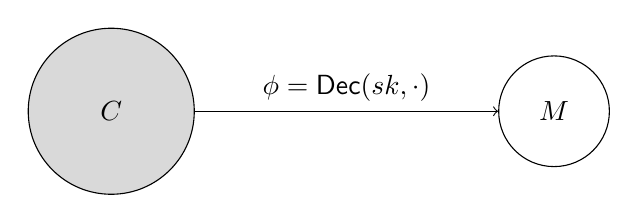
\begin{tikzpicture}
    \node[circlenode, name=C, minimum width=6em, fill=gray!30] {$C$}; 
    \node[circlenode, name=M, minimum width=4em, right of = C, xshift=16em] {$M$};
    \draw (C) edge[->] node[above] {$\phi = \mathsf{Dec}(sk, \cdot)$} (M); 
\end{tikzpicture}
\end{center}


\subsection{密钥封装机制}\label{subsec:KEM}
主流的公钥加密方案基于数论或者格基困难问题构造. 
基于数论问题的公钥加密方案因需要进行高精度算术运算导致加解密速率较低, 基于格基困难问题的公钥加密方案存在公钥和密文尺寸较大的问题. 
而对称加密方案因其功能简单, 仅需异或等逻辑运算即可完成, 且硬件支持良好(如定制的指令), 
因此在较公钥加密具有较大的性能优势, 在加密长明文的场景下更为显著. 

如何解决公钥加密在加密长消息时的性能短板呢? 解决思路是混合加密(hybrid encryption), 
朴素的实现方式是PKE+SKE, 如图~\ref{figure:PKE+SKE}所示: 
\begin{enumerate}
\item 发送方首先随机选择对称密钥$k$, 调用公钥加密算法用接收方的公钥$pk$加密$k$得到$c$, 
	再调用对称加密算法用$k$加密明文$m$得到$c_1$, 最终的密文$(c, c')$. 

\item 接收方在接收到密文$(c, c')$后, 首先使用私钥$sk$解密$c$恢复对称密钥$k$, 再使用$k$解密$c'$. 
\end{enumerate}     

\begin{figure}[!hbtp]
\begin{center}
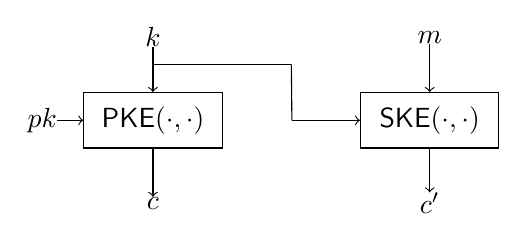
\begin{tikzpicture}
    \node [name=enc1, rectanglenode, minimum width=5em, minimum height=2em] {$\mathsf{PKE}(\cdot, \cdot)$}; 
    \node [name=k, textnode, above of=enc1, yshift=3em] {$k$}; 
    \node [name=c1, textnode, below of=enc1, yshift=-3em] {$c$}; 
    \node [name=pk, textnode, left of=enc1, xshift=-4em] {$pk$}; 
    \draw (pk) edge[->]  (enc1);
    \draw (k) edge[->] (enc1);
    \draw (enc1) edge[->] (c1);

    \node [name=enc2, rectanglenode, minimum width=5em, minimum height=2em, right of=enc1, xshift=10em] {$\mathsf{SKE}(\cdot, \cdot)$}; 
    \node [name=m, textnode, above of=enc2, yshift=3em] {$m$}; 
    \node [name=c2, textnode, below of=enc2, yshift=-3em] {$c'$}; 

    \draw (m) edge[connect] (enc2);
    \draw (enc2) edge[connect] (c2);

    \draw ($(enc1.north)+(0em, 1em)$) edge[-] ($(enc1.north)+(5em, 1em)$);
    \draw ($(enc1.north)+(5em, 1em)$) edge[-] ($(enc1.east)+(2.5em, 0em)$);
    \draw ($(enc1.east)+(2.5em, 0em)$) edge[->] (enc2);
\end{tikzpicture}
\end{center}
\caption{混合加密: PKE+SKE}\label{figure:PKE+SKE}
\end{figure}


混合加密方法既保留了公钥加密的功能性, 同时性能几乎与对称加密相当, 因此是公钥加密加密长明文时的通用范式. 
Cramer和Shoup~\cite{CS-EUROCRYPT-2002}观察到公钥加密在混合加密范式中起到的关键作用是发送方向接收方传输对称密钥, 
而传递的方式并非必须是加解密. 基于该观察, Cramer和Shoup提出了``密钥封装-数据封装''范式, 
简称为KEM-DEM(key/data-encapsulation mechanism), 该范式可以看作是混合加密的另一种实现方式, 如图~\ref{figure:KEM+DEM}所示.  
顾名思义, KEM-DEM范式包含KEM和DEM两个组件, DEM可以粗略的等同为对称加密, KEM是该范式的核心. 
简言之, KEM与PKE的不同在于发送方不再先显式选择对称密钥再加密, 而是封装一个随机的对称密钥. 

\begin{figure}[!hbtp]
\begin{center}
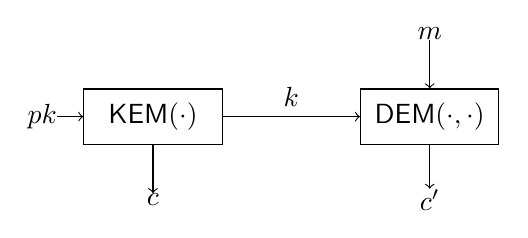
\begin{tikzpicture}
    \node [name=enc1, rectanglenode, minimum width=5em, minimum height=2em] {$\mathsf{KEM}(\cdot)$}; 
    \node [name=c1, textnode, below of=enc1, yshift=-3em] {$c$}; 
    \node [name=pk, textnode, left of=enc1, xshift=-4em] {$pk$}; 
    \draw (pk) edge[->]  (enc1);
    \draw (enc1) edge[->] (c1);

    \node [name=enc2, rectanglenode, xshift=10em, right of=enc1, minimum width=5em, minimum height=2em] {$\mathsf{DEM}(\cdot, \cdot)$}; 
    \node [name=m, textnode, above of=enc2, yshift=3em] {$m$}; 
    \node [name=c2, textnode, below of=enc2, yshift=-3em] {$c'$}; 

    \draw (m) edge[->] (enc2);
    \draw (enc2) edge[->] (c2);

    \draw (enc1) edge[->] node [auto] {$k$} (enc2);
\end{tikzpicture}
\end{center}
\caption{混合加密: KEM+DEM}\label{figure:KEM+DEM}
\end{figure}

\begin{definition}[密钥封装机制]
正式的, KEM由以下的四个多项式时间组成: 
\begin{itemize}
\item $\mathsf{Setup}(1^\kappa)$: 系统生成算法以安全参数$1^\lambda$为输入, 输出系统公开参数$pp$, 其中$pp$包含对
	公钥空间$PK$、私钥空间$SK$、对称密钥空间$K$和密文空间$C$的描述. 
	该算法由可信第三方生成并公开, 系统中的所有用户共享, 所有算法均将$pp$作为输入.  
	当上下文明确时, 常常为了行文简洁省去$pp$. 

\item $\mathsf{KeyGen}(pp)$: 密钥生成算法以系统公开参数$pp$为输入, 输出一对公/私钥对$(pk, sk)$, 其中公钥公开, 私钥秘密保存. 

\item $\mathsf{Encaps}(pk; r)$: 封装算法以公钥$pk \in PK$为输入, 输出对称密钥$k \in K$和封装密文$c \in C$.  

\item $\mathsf{Decaps}(sk, c)$: 解封装算法以私钥$sk \in SK$和密文$c \in C$为输入, 
	输出对称密钥$k \in K$或者$\bot$表示封装密文非法. 解封装算法通常为确定性算法. 
\end{itemize}
\end{definition}

\begin{remark}
在KEM中, 对称密钥$k$起到的作用是在发送方和接收方之间建立安全的会话信道, 因此也常称为会话密钥. 
\end{remark}

\begin{trivlist}
\item \textbf{正确性.} 该性质保证KEM的功能性, 即使用私钥可以正确恢复出封装密文所封装的会话密钥. 
正式的, 对于任意会话密钥$k \in K$, 有:
\begin{equation}\label{equation:KEM-correctness}
	\Pr[\mathsf{Decaps}(sk, c) = k: (c, k) \leftarrow \mathsf{Encaps}(pk)] = 1 - \mathsf{negl}(\kappa).
\end{equation}
公式~\eqref{equation:KEM-correctness}的概率建立在$\mathsf{Setup}(1^\kappa) \rightarrow pp$、
$\mathsf{KeyGen}(pp) \rightarrow (pk, sk)$和$\mathsf{Encaps}(pk) \rightarrow (c, k)$的随机带上. 
如果上述概率严格等于1, 则称KEM方案满足完美正确性. 
\end{trivlist}

\begin{trivlist}
\item \textbf{安全性.} 定义KEM敌手$\mathcal{A}$的优势函数如下: 
\begin{displaymath}
\AdvA(\kappa) = \Pr \left[ \beta' = \beta:~
	\begin{array}{ll}
		& pp \leftarrow \mathsf{Setup}(1^\lambda); \\		
		& (pk, sk) \leftarrow \mathsf{KeyGen}(pp);\\
        & (c^*, k_0^*) \leftarrow \mathsf{Encaps}(pk), k_1^* \sample K;\\
		& \beta \sample \{0,1\};\\ 
        & \beta' \leftarrow \mathcal{A}^{\blue{\Odecaps(\cdot)}}(pp, pk, c^*, k_\beta^*);
	\end{array} 
\right] - \frac{1}{2},
\end{displaymath}
在上述定义中, $\Odecaps(\cdot)$表示解封装谕言机, 其在接收到密文$c$的询问后输出$\mathsf{Decaps}(sk, c)$. 
如果任意的PPT敌手$\mathcal{A}$在上述游戏中的优势函数均为可忽略函数, 则称KEM方案是IND-CPA安全的;   
如果任意的PPT敌手在可自适应访问$\Odecaps(\cdot)$的情形下仍仅具有可忽略优势, 则称KEM方案是IND-CCA安全的. 
\end{trivlist}

下面给出安全性定义的一些注记: 
\begin{itemize}
\item KEM的安全游戏中分阶段定义敌手不再必要, 因为挑战密文的生成不受敌手控制, 
	正是这点不同使得KEM的安全性定义要比PKE的安全性定义简单. 

\item 为了避免定义无意义, 在IND-CCA的安全游戏中禁止敌手向$\Odecaps(\cdot)$询问挑战密文$c^*$.  
\end{itemize}

\magenta{补充DEM部分和KEM+DEM的安全性组合}

\subsection{两类混合加密范式的比较}
以上两种混合方法的共性都是首先生成对称密钥, 再利用对称密钥加密明文, 因此效率方面的差异体现在第一阶段. 
PKE+SKE范式的非对称部分是先选择一个随机的密钥$k$, 再使用PKE对其加密得到$c$, 而KEM+DEM范式的非对称部分是两步并做一步完成. 
如果使用PKE-SKE范式, 密文$c$必然存在密文扩张, 这是由概率加密的本质决定的; 
而如果使用KEM+DEM的方法, 密文$c$相比$k$可能不存在扩张, 原因是此时$c$是对$k$的封装, 而非加密. 
综上, 使用KEM代替PKE, 不仅能够缩减整体密文尺寸, 也能够提升效率. 
\begin{remark}
通常KEM要比PKE构造简单, 这是因为KEM可以看作功能受限的PKE, 因为其只允许加密随机的明文.
\end{remark}

相比效率提升, KEM-DEM的理论价值更大. 首先, KEM-DEM范式实现了对PKE的功能解耦, 将PKE中的非对称内核抽取出来凝练为KEM, 意义如下:
\begin{itemize}
\item KEM-DEM范式极大简化了PKE的可证明安全. 我们只需证明KEM和DEM满足一定性质即可. 
	对比安全模型即可发现, 对于PKE有CPA/CCA1/CCA三个依次增强的安全性, 而KEM只有CPA/CCA两个依次增强的安全性. 
	最关键的是: 在PKE中敌手A对挑战密文$c^*$有一定的控制能力, 而KEM中$c^*$完全由挑战者控制, 
	这一区别使得KEM安全证明中的归约算法更容易设计.

\item KEM-DEM范式有助于简化PKE的设计. 该范式将PKE的设计任务简化为对应的KEM, 
	在后面的章节中可以看到, 在设计高等级安全的PKE时, 仅需设计满足相应安全性的KEM即可.

\item KEM-DEM范式有助于洞悉PKE本质. 该范式揭示了构造PKE的核心机制在于构造KEM. 
	后续的章节揭示了KEM的本质是公开可求值的伪随机函数, 是伪随机函数在minicrypt中的对应. 
	认识到这一点后, 不仅可以将几乎所有公钥加密的构造统一在同一框架下, 还可以将SKE和PKE的构造在伪随机函数的视角下实现高度统一. 
\end{itemize}

\begin{remark}
目前, 格基的KEM设计仍是PKE-SKE的方式, 显得不够灵巧纯粹, 如何设计精巧纯粹的格基KEM是很有挑战意义的研究课题. 
\end{remark}

\chapter{经典公钥加密方案回顾}
\section{基于数论问题的经典方案}
\subsection{Goldwasser-Micali PKE}
Goldwasser和Micali~\cite{GM-JCSS-1984}在1984年基于QR假设构造出首个可证明安全的公钥加密方案. 
该方案仅能加密一比特消息, 设计的思想可类比编码: 当明文为0时, 随机选取二次剩余元素作为密文; 
当明文为1时, 随机选取Jacobi符号为+1的非二次剩余元素作为密文.  
\begin{construction}[Goldwasser-Micali PKE]
\begin{itemize}
\item $\mathsf{Setup}(1^\kappa)$: 全局参数生成$pp$, 包含对明文空间$M = \{0,1\}$的描述. 

\item $\mathsf{KeyGen}(pp)$: 从$pp$中解析出$\kappa$, 运行$\mathsf{GenModulus}(1\kappa) \rightarrow (N, p, q)$, 
	随机选取$z \in \mathcal{QNR}_N^{+1}$, 输出公钥$pk = (N, z)$和私钥$sk = (p, q)$. 

\item $\mathsf{Encrypt}(pk, m)$: 以公钥$pk = (N, z)$和明文$m \in \{0,1\}$为输入, 随机选择$x \sample \mathbb{Z}_N^*$, 
	输出密文$c = z^m \cdot x^2 \bmod N$. 

\item $\mathsf{Decrypt}(sk, c)$: 以私钥$sk = (p, q)$和密文$c$为输入, 利用私钥判定$c$是否是模$N$的二次剩余. 
	若是, 输出0; 否则输出1.  
\end{itemize}
\end{construction} 

Goldwasser-Micali PKE的正确性显然, 安全性由以下定理保证. 
\begin{theorem}\label{theorem:Goldwasser-Micali-PKE-CPA}
如果QR假设成立, 那么Goldwasser-Micali PKE是IND-CPA安全的. 
\end{theorem}

\begin{proof}
令$S_i$表示敌手在$\text{Game}_i$中成功概率. 以游戏序列的方式组织证明如下: 

\begin{trivlist}
\item $\text{Game}_0$: 该游戏是标准的IND-CPA游戏, 挑战者$\mathcal{CH}$和敌手$\mathcal{A}$交互如下: 
\begin{itemize}
	\item 初始化: $\mathcal{CH}$运行$\mathsf{Setup}(1^\kappa)$生成公开参数$pp$, 
		同时运行$\mathsf{KeyGen}(pp)$生成公私钥对$pk = (N, z)$和$sk = (p, q)$. 
		$\mathcal{CH}$将$(pp, pk)$发送给$\mathcal{A}$. 

	\item 挑战: $\mathcal{A}$选择$m_0, m_1 \in \mathbb{G}$并发送给$\mathcal{CH}$. 
		$\mathcal{CH}$选择随机比特$\beta \in \{0,1\}$, 随机选择$x \in \mathbb{Z}_N^*$, 
		计算$c^* = z^{m_\beta} \cdot x^2 \bmod N$并发送给$\mathcal{A}$.  

	\item 猜测: $\mathcal{A}$输出对$\beta$的猜测$\beta'$. $\mathcal{A}$成功当且仅当$\beta' = \beta$. 
\end{itemize} 
根据定义, 我们有: 
\begin{equation*}
	\AdvA(\kappa) = |\Pr[S_0] - 1/2|
\end{equation*}

\item $\text{Game}_1$: 与$\text{Game}_0$的唯一不同在于密钥对的生成方式, 
	$\mathcal{CH}$将$pk$中元素$z$的选取由Jacobi符号为+1的随机非二次剩余元素切换为随机二次剩余元素. 
	在$\text{Game}_1$中, 无论$m_\beta$是0还是1, 密文分布均是$\mathcal{QR}_N$上的均匀分布, 完美掩盖了$\beta$的信息. 
	因此, 即使对于拥有无穷计算能力的敌手, 我们也有:   
\begin{equation*}
	\AdvA(\kappa) = |\Pr[S_1] - 1/2| = 0
\end{equation*}
\end{trivlist}

\begin{lemma}
如果QR假设成立, 那么对于任意PPT敌手我们均有$|\Pr[S_0]-\Pr[S_1]| \leq \mathsf{negl}(\kappa)$. 
\end{lemma}

\begin{proof}
证明的思路是反证. 若存在PPT敌手$\mathcal{A}$在$\text{Game}_0$和$\text{Game}_1$中成功的概率之差不可忽略, 
则可构造出PPT算法$\mathcal{B}$打破QR困难问题. 
令$\mathcal{B}$的QR挑战实例为$(N, z)$, $\mathcal{B}$的目标是区分挑战实例$z$选自$\mathcal{QNR}_N^{+1}$还是$\mathcal{QR}_N$上的均匀分布.  
为此$\mathcal{B}$扮演IND-CPA游戏中的挑战者与$\mathcal{A}$交互如下: 
\begin{itemize}
	\item 初始化: $\mathcal{B}$根据它的挑战实例生成$pp$, 令$pk = (N, z)$, 将$(pp, pk)$发送给$\mathcal{A}$.   

	\item 挑战: $\mathcal{A}$选择$m_0, m_1 \in \mathbb{G}$并发送给$\mathcal{B}$.  
		$\mathcal{B}$随机选择$\beta \sample \{0,1\}$, 随机选取$x \in \mathbb{Z}_N^*$
		设置$c^* = z^{m_\beta} \cdot x^2$并发送给$\mathcal{A}$.   

	\item 猜测: $\mathcal{A}$输出对$\beta$的猜测$\beta'$. 如果$\beta' = \beta$, $\mathcal{B}$输出1. 
\end{itemize} 
对上述交互分析可知, 如果$z \sample \mathcal{QNR}_N^{+1}$, 那么$\mathcal{B}$完美的模拟了$\text{Game}_0$; 
如果$z \sample \mathcal{QR}_N$, 那么$\mathcal{B}$完美的模拟了$\text{Game}_1$. 
因此, $\mathcal{B}$解决QR挑战的优势$\mathsf{Adv}_\mathcal{B}^\text{QR}(\kappa) = |\Pr[S_0]-\Pr[S_1]|$. 
如果QR假设成立, 我们有$|\Pr[S_0]-\Pr[S_1]| \leq \mathsf{negl}(\kappa)$. 
\end{proof}
综上, 定理得证. \qed
\end{proof}

\subsection{Rabin PKE}
Rabin~\cite{Rabin-TechReport-1979}在1979年基于SQR假设构造出$\mathcal{QR}_N$上的单向陷门置换$f_N \define [x^2 \bmod N]$, 
称为Rabin TDP. 可以证明, 最低有效位(lsb, least significant bit)函数是Rabin TDP的hardcore谓词. 
基于Rabin TDP, 可以构造公钥加密方案如下: 
\begin{definition}[Rabin PKE]
\begin{itemize}
\item $\mathsf{Setup}(1^\kappa)$: 全局参数生成$pp$, 包含对明文空间$M = \{0,1\}$的描述. 

\item $\mathsf{KeyGen}(pp)$: 从$pp$中解析出$\kappa$, 运行$\mathsf{GenModulus}(1\kappa) \rightarrow (N, p, q)$, 
	其中$N$是Blum整数. 输出公钥$pk = N$和私钥$sk = (p, q)$. 

\item $\mathsf{Encrypt}(pk, m)$: 以公钥$pk = N$和明文$m \in \{0,1\}$为输入, 随机选择$x \sample \mathcal{QR}_N$, 
	计算$c_0 = x^2 \bmod N$, 计算$c_1 = m \oplus \mathsf{lsb}(x)$, 输出$c = (c_0, c_1)$作为密文. 

\item $\mathsf{Decrypt}(sk, c)$: 以私钥$sk = (p, q)$和密文$c = (c_0, c_1)$为输入, 
	计算$x$满足$x^2 = c_0 \bmod N$, 输出$m' = c_1 \oplus \mathsf{lsb}(x)$.
\end{itemize}
\end{definition}

Rabin PKE的正确性由$f_N \define [x^2 \bmod N]$是陷门置换这一事实保证, IND-CPA安全性由陷门置换的单向性保证. 
\section{基于离散对数类问题的经典方案}
\subsection{ElGamal PKE}
1985年, ElGamal~\cite{ElGamal-IEEE-IT-1985}基于Diffie-Hellman构造了ElGamal PKE方案. 
该方案设计简洁精巧, 对后续的研究有深远的影响. 
\begin{definition}[ElGamal PKE]
\begin{itemize}
\item $\mathsf{Setup}(1^\kappa)$: 运行$\mathsf{GenGroup}(1^\kappa) \rightarrow (\mathbb{G}, q, g)$, 
	输出$pp$包含循环群描述, 同时包含对公钥空间$PK = \mathbb{G}$、私钥空间$SK = \mathbb{Z}_q$、
	明文空间$M = \mathbb{G}$和密文空间$C = \mathbb{G}^2$. 

\item $\mathsf{KeyGen}(pp)$: 随机选取$sk \in \mathbb{Z}_q$作为私钥, 计算公钥$pk:= g^{sk}$. 
  
\item $\mathsf{Encrypt}(pk, m)$: 以公钥$pk$和明文$m \in \mathbb{G}$为输入, 
	随机选择$r \sample \mathbb{Z}_q$, 计算$c_0 = g^r$, $c_1 = pk^r \cdot m$, 输出密文$c = (c_1, c_2) \in C$. 

\item $\mathsf{Decrypt}(sk, c)$: 以私钥$sk$和密文$c = (c_0, c_1)$为输入, 输出$m':= c_1/c_0^{sk}$.
\end{itemize}
\end{definition}

\begin{trivlist}
\item \textbf{正确性.} 以下公式~\ref{equation:ElGamal-PKE-correctness}说明方案具有完美正确性: 
\begin{equation}\label{equation:ElGamal-PKE-correctness}
	m' = c_1/c_0^{sk} = pk^r \cdot m/(g^r)^{sk} = m
\end{equation}
\end{trivlist}

\begin{theorem}\label{theorem:ElGamal-PKE-CPA}
如果DDH假设成立, 那么ElGamal PKE是IND-CPA安全的. 
\end{theorem}

\begin{proof}
令$S_i$表示敌手在$\text{Game}_i$中成功概率. 以游戏序列的方式组织证明如下: 

\begin{trivlist}
\item $\text{Game}_0$: 该游戏是标准的IND-CPA游戏, 挑战者$\mathcal{CH}$和敌手$\mathcal{A}$交互如下: 
\begin{itemize}
	\item 初始化: $\mathcal{CH}$运行$\mathsf{Setup}(1^\kappa)$生成公开参数$pp$, 
		同时运行$\mathsf{KeyGen}(pp)$生成公私钥对$(pk, sk)$. $\mathcal{CH}$将$(pp, pk)$发送给$\mathcal{A}$. 

	\item 挑战: $\mathcal{A}$选择$m_0, m_1 \in \mathbb{G}$并发送给$\mathcal{CH}$. 
		$\mathcal{CH}$选择随机比特$\beta \in \{0,1\}$, 随机选择$r \in \mathbb{Z}_q$, 
		计算$c^* = (g^r, pk^r \cdot m_\beta)$并发送给$\mathcal{A}$.  

	\item 猜测: $\mathcal{A}$输出对$\beta$的猜测$\beta'$. $\mathcal{A}$成功当且仅当$\beta' = \beta$. 
\end{itemize} 
根据定义, 我们有: 
\begin{equation*}
	\AdvA(\kappa) = |\Pr[S_0] - 1/2|
\end{equation*}

\item $\text{Game}_1$: 与$\text{Game}_0$的唯一不同在于挑战密文的生成方式, 
	$\mathcal{CH}$不再计算$pk^r$作为会话密钥掩蔽$m_\beta$, 而是随机选取$z \sample \mathbb{Z}_q$, 用$g^z$作为会话密钥掩蔽$m_\beta$. 
	挑战密文$c^* = (g^r, g^z \cdot m_\beta)$. 在$\text{Game}_1$中, 由于$r$和$z$均有挑战者从$\mathbb{Z}_q$中独立随机选取, 
	因此挑战密文$c^*$在$\mathbb{G} \times \mathbb{G}$上均匀分布, 完美掩盖了$\beta$的信息. 
	因此, 即使对于拥有无穷计算能力的敌手, 我们也有:   
\begin{equation*}
	\AdvA(\kappa) = |\Pr[S_1] - 1/2| = 0
\end{equation*}
\end{trivlist}

\begin{lemma}
如果DDH假设成立, 那么对于任意PPT敌手我们均有$|\Pr[S_0]-\Pr[S_1]| \leq \mathsf{negl}(\kappa)$. 
\end{lemma}

\begin{proof}
证明的思路是反证. 若存在PPT敌手$\mathcal{A}$在$\text{Game}_0$和$\text{Game}_1$中成功的概率差不可忽略, 
则可构造出PPT算法$\mathcal{B}$打破DDH困难问题. 
令$\mathcal{B}$的DDH挑战实例为$(g, g^a, g^b, g^c)$, $\mathcal{B}$的目标是区分挑战实例是DDH四元组还是随机四元组.  
为此$\mathcal{B}$扮演IND-CPA游戏中的挑战者与$\mathcal{A}$交互如下: 
\begin{itemize}
	\item 初始化: $\mathcal{B}$根据它的挑战实例生成$pp$, 令$pk = g^a$, 将$(pp, pk)$发送给$\mathcal{A}$. 
		注意, $\mathcal{B}$并不知晓$a$ (这是符合逻辑的, 不然归约无意义).  

	\item 挑战: $\mathcal{A}$选择$m_0, m_1 \in \mathbb{G}$并发送给$\mathcal{B}$.  
		$\mathcal{B}$随机选择$\beta \sample \{0,1\}$, 
		设置$c^* = (g^b, g^c \cdot m_\beta)$并发送给$\mathcal{A}$. 该设定隐式的设定$r = b$.   

	\item 猜测: $\mathcal{A}$输出对$\beta$的猜测$\beta'$. 如果$\beta' = \beta$, $\mathcal{B}$输出1. 
\end{itemize} 
对上述交互分析可知, 如果$c = ab$, 那么$\mathcal{B}$完美的模拟了$\text{Game}_0$; 如果$c$在$\mathbb{Z}_q$中随机选择, 
那么$\mathcal{B}$完美的模拟了$\text{Game}_1$. 
因此, $\mathcal{B}$解决DDH挑战的优势$\mathsf{Adv}_\mathcal{B}^\text{DDH}(\kappa) = |\Pr[S_0]-\Pr[S_1]|$. 
如果DDH假设成立, 我们有$|\Pr[S_0]-\Pr[S_1]| \leq \mathsf{negl}(\kappa)$. 
\end{proof}
综上, 定理得证. \qed
\end{proof}

\begin{note}[具有实际应用价值的同态]
ElGamal PKE构建在$q$阶循环群$\mathbb{G} = \langle g \rangle$上, 明文空间是$\mathbb{G}$, 使用公钥$pk$对明文$m$的加密所得密文为$(g^r, pk^r \cdot m)$. 
容易验证, ElGamal PKE相对于$\mathbb{G}$中的群运算``$\cdot$''同态, 然而, 这种类型的同态并无实际意义, 
现实应用中需要的是相对于$\mathbb{Z}_q$上的模加运算``+''同态. 
面向实际需求, ISO/IEC标准化了exponential ElGamal PKE方案. 
该方案同样构建在$q$阶循环群$\mathbb{G} = \langle g \rangle$上, 所不同的是明文空间设定为$\mathbb{G}$的自然同构$\mathbb{Z}_q$, 
使用公钥$pk$对明文$m$加密时, 首先计算$m$的自然同构映射结果$g^m$, 再如常加密, 最终密文为$(g^r, pk^r \cdot g^m)$. 
容易验证, exponential ElGamal相对于$\mathbb{Z}_q$中的``+''运算同态. 
\end{note}

\subsection{Twisted ElGamal PKE}
近半个世纪, 随着网络技术的飞速发展, 计算模式逐渐由集中式迁移分布式. 新型计算模式对加密方案的需求也从单一的机密性保护扩展到对隐私计算的支持. 
上一节注记中提到的Exponential ElGamal PKE支持$\mathbb{Z}_p$上的模加运算``+''同态, 适用于密态计算场景. 
在区块链和机器学习等涉及恶意敌手的计算场景中, 还常需要以隐私保护的方式证明密文加密的明文满足声称的约束关系, 特别的, 在指定的区间内, 
我们称之为零知识密态区间范围证明. 

零知识密态区间范围证明又可以根据证明者的角色分为两类: 
\begin{enumerate}
    \item 证明者为密文生成方: 证明者知晓加密随机数$r$和加密消息$m$. 
    \item 证明者为密文接收方: 证明者知晓解密私钥$sk$和加密消息$m$.  
\end{enumerate}
我们称上面两种情形下完成密态证明的组件为Gadget-1和Gadget-2. 下面详细讨论Gadget-1的构造, Gadget-2的设计可以通过重加密技术归结为Gadget-2. 

当前最高效的零知识区间范围证明系统是构建在离散对数群上的Bulletproof~\cite{Bunz-BulletProof-SP-2018}, 其接受的断言类型为Pedersen承诺. 
尽管exponential ElGamal PKE密文的第二项$pk^r \cdot g^m$也是Pedersen承诺的形式, 
但是若证明者为密文生成方, 则其知晓承诺密钥$(pk, g)$之间的离散对数关系, 因此无法调用Bulletproof完成证明(合理性得不到保证), 
如图~\ref{figure:ElGamal-cannot-link-Bulletproof}所示. 

\begin{figure}[!hbtp]
\begin{center}
\begin{tikzpicture}
    \node [textnode, name=ElGamal] {ElGamal};
    \node [textnode, name=C1, below of=ElGamal, xshift=-3em, yshift=-5em] {$g^r$};
    \node [textnode, name=C2, below of=ElGamal, xshift=3em, yshift=-5em] {$pk^r g^m$};
    \draw ($(ElGamal.south)$) edge[-] (C1); 
    \draw ($(ElGamal.south)$) edge[-] (C2);  
    \node[ellipse callout, color=red, draw, above of = C2, xshift=2em, yshift = 1em, 
        callout absolute pointer={(C2.north)}, font=\scriptsize] {oblivious\\[-0.5em]trapdoor};  

    \node [shapenode, right of = ElGamal, xshift=32em, fill=blue!20, yshift=-2.5em, minimum width=6em, minimum height=7em] {};
    \node [textnode, name=Bulletproof, right of = ElGamal, xshift=32em] {Bulletproof};
    \node [textnode, name=input, below of = Bulletproof, yshift=-5em] {$g^r h^m$};
    \node [textnode, above of = input, yshift=1.5em] {断言类型}; 

    \draw (C2) edge[-] node[midway] {\redcross} (input.west);  
\end{tikzpicture}
\end{center}
\caption{ElGamal无法与Bulletproof直接对接}\label{figure:ElGamal-cannot-link-Bulletproof}
\end{figure}

解决该问题有两种技术手段: 
\begin{enumerate}
\item 文献~\cite{Quisquis-ASIACRYPT-2019}中的方法: 证明者首先使用NIZKPoK证明其知晓密文的随机数和消息, 
    再引入新的Pedersen承诺作为桥接, 并设计$\Sigma$协议证明新承诺的消息与明文的一致性(注: 该Sigma协议可与第一步的NIZKPoK协议合并设计), 再调用Bulletproof对桥接承诺进行证明, 如图~\ref{figure:ElGamal-bridge-Bulletproof}所示. 
    该方法的缺点是需要引入桥接承诺的额外的$\Sigma$协议, 增大了证明和验证的开销. 

\begin{figure}[!hbtp]
\begin{center}
\begin{tikzpicture}
    \node [textnode, name=ElGamal] {ElGamal};
    \node [textnode, name=C1, below of=ElGamal, xshift=-3em, yshift=-5em] {$g^r$};
    \node [textnode, name=C2, below of=ElGamal, xshift=3em, yshift=-5em] {$pk^r g^m$};
    \draw ($(ElGamal.south)$) edge[-] (C1); 
    \draw ($(ElGamal.south)$) edge[-] (C2);  

    \draw (C1.south) [decorate, decoration={brace, mirror, raise=2pt, amplitude=8pt}] -- (C2.south);
    \node [shapenode, draw = none, fill = gray!30, name=NIZKPoK, below of = ElGamal, yshift=-7.5em] {$\Sigma$ protocol}; 
    \node [textnode, right of=NIZKPoK, xshift=9em] {proof of knowledge $(r, m)$}; 

    \node [shapenode, right of = ElGamal, xshift=32em, fill=blue!20, yshift=-2.5em, minimum width=6em, minimum height=7em] {};
    \node [textnode, name=Bulletproof, right of = ElGamal, xshift=32em] {Bulletproof};
    \node [textnode, name=input, below of = Bulletproof, yshift=-5em] {$g^r h^m$};
    \node [textnode, above of = input, yshift=1.5em] {断言类型}; 

    \node [shapenode, draw = none, fill = orange, name=sigma, right of = C2, xshift=10em] {$\Sigma$ protocol}; 
    \node [textnode, above of=sigma, yshift=2em] {proof of consistency}; 
    \node [shapenode, draw=none, fill = darkgreen!30, name=commitment, right of = sigma, xshift=10em, minimum width=4em] 
        {$g^{r'} h^m$};
    \node [textnode, above of=commitment, yshift=2em] {Pedersen commitment};  

    \draw (commitment) edge[-] (input); 
    \draw (sigma) edge[->] (C2); 
    \draw (sigma) edge[->] (commitment); 
\end{tikzpicture}
\end{center}
\caption{ElGamal PKE的密态区间范围证明组件Gadget-1之设计方法一}\label{figure:ElGamal-bridge-Bulletproof}
\end{figure}

\item 文献~\cite{Zether-FC-2020}中的方法: 结合待证明的ElGamal PKE密文对Bulletproof进行重新设计, 
    使用量身定制的$\Sigma$-Bulletproof完成证明, 如图~\ref{figure:ElGamal-dissect-Bulletproof}所示. 
	该方法的缺点是需要对Bulletproof进行定制化的改动, 不具备模块化特性.  
\begin{figure}[!hbtp]
\begin{center}
\begin{tikzpicture}
    \node [textnode, name=ElGamal] {ElGamal};
    \node [textnode, name=C1, below of=ElGamal, xshift=-3em, yshift=-5em] {$g^r$};
    \node [textnode, name=C2, below of=ElGamal, xshift=3em, yshift=-5em] {$pk^r g^m$};
    \draw ($(ElGamal.south)$) edge[-] (C1); 
    \draw ($(ElGamal.south)$) edge[-] (C2);  


    \node [shapenode, right of = ElGamal, xshift=32em, fill=blue!20, yshift=-2.5em, minimum width=6em, minimum height=7em] {};
    \node [textnode, name=Bulletproof, right of = ElGamal, xshift=32em] {Bulletproof};
    \node [textnode, name=input, below of = Bulletproof, yshift=-5em] {$g^r h^m$};
    \node [textnode, above of = input, yshift=1.5em] {断言类型}; 

    \node [shapenode, right of = ElGamal, xshift=14em, fill=magenta!30, yshift=-2.5em, minimum width=6em, minimum height=7em] {}; 
    \node [textnode, name=sigma-bullet, right of = ElGamal, xshift=14em] {$\Sigma$-Bullet};
    \node [textnode, name=input2, below of = sigma-bullet, yshift=-5em] {};
    \draw (C2) edge[->] ($(input2.west)+(-3em, 0em)$); 
    \draw ($(input.west)+(-1.8em, 2.5em)$) edge[->] ($(input2.east)+(3em, 2.5em)$);  
\end{tikzpicture}
\end{center}
\caption{ElGamal PKE的密态区间范围证明组件Gadget-1之设计方法二}\label{figure:ElGamal-dissect-Bulletproof}
\end{figure}
\end{enumerate}

上述两种技术手段均存在不足. 为了解决这一问题, Chen等~\cite{Chen-ESORICS-2020}对exponential ElGamal PKE进行变形扭转, 
将封装密文$g^r$与会话密钥$pk^r$的位置对调, 同时更改同构映射编码的基底, 得到twisted ElGamal PKE. 

\begin{definition}[Twisted ElGamal PKE]
\begin{itemize}
\item $\mathsf{Setup}(1^\kappa)$: 运行$\mathsf{GenGroup}(1^\kappa) \rightarrow (\mathbb{G}, q, g)$, 
	随机选取$\mathbb{G}$的另一生成元$h$,  
	输出$pp$包含循环群和$h$的描述, 同时包含对公钥空间$PK = \mathbb{G}$、私钥空间$SK = \mathbb{Z}_q$、
	明文空间$M = \mathbb{Z}_q$和密文空间$C = \mathbb{G}^2$. 

\item $\mathsf{KeyGen}(pp)$: 随机选取$sk \in \mathbb{Z}_q$作为私钥, 计算公钥$pk:= g^{sk}$. 
  
\item $\mathsf{Encrypt}(pk, m)$: 以公钥$pk$和明文$m \in \mathbb{Z}_q$为输入, 
	随机选择$r \sample \mathbb{Z}_q$, 计算$c_0 = pk^r$, $c_1 = pk^r \cdot h^m$, 输出密文$c = (c_1, c_2) \in C$. 

\item $\mathsf{Decrypt}(sk, c)$: 以私钥$sk$和密文$c = (c_0, c_1)$为输入, 输出$m':= \log_h c_1/c_0^{sk^{-1}}$.
\end{itemize}
\end{definition} 

\begin{trivlist}
\item \textbf{正确性.} 以下公式~\ref{equation:twisted-ElGamal-PKE-correctness}说明方案具有完美正确性: 
\begin{equation}\label{equation:twisted-ElGamal-PKE-correctness}
    c_1/c_0^{sk^{-1}} = g^r \cdot h^m/(pk^r)^{sk^{-1}} = h^m
\end{equation}
\end{trivlist}

\begin{theorem}\label{theorem:twisted-ElGamal-PKE-CPA}
如果DDH假设成立, 那么twisted ElGamal PKE是IND-CPA安全的. 
\end{theorem}
证明与标准的ElGamal PKE证明类似, 我们留给作者作为练习. 

\begin{note}
为获得$\mathbb{Z}_q$上的加法同态, exponential ElGamal PKE和twisted ElGamal PKE均将明文空间设定为$\mathbb{Z}_q$, 加密时必须先进行同构编码, 
解密时则在最后需要进行解码. 解码的过程等同于求解离散对数, 因此为了确保解密高效, 必须将明文空间限制在较小的范围内, 如$[0, 2^{40}]$. 
\end{note} 

\begin{trivlist}
\item \textbf{零知识证明友好特性.} 新的加密方案与exponential ElGamal PKE的性能和安全性相当, 
    同样满足$\mathbb{Z}_q$上的模加同态. 特别的, 密文的第二部分恰好是标准的Pedersen承诺形态(承诺密钥陷门未知), 
    可无缝对接Bulletproof等一系列断言类型为Pedersen commitment的区间范围证明, 如图~\ref{figure:twisted-ElGamal-Bulletproof}所示. 
    我们称公钥加密方案的这种性质为零知识证明友好. 
\end{trivlist}

\begin{figure}[!hbtp]
\begin{center}
\begin{tikzpicture}
    \node [textnode, name=twisted_ElGamal] {twisted ElGamal};
    \node [textnode, name=C1, below of=twisted_ElGamal, xshift=-3em, yshift=-3em] {$\blue{g^r}$};
    \node [textnode, name=C2, below of=twisted_ElGamal, xshift=3em, yshift=-3em] {$\red{pk^r} g^m$};
    \draw ($(ElGamal.south)$) edge[-, dashed] (C1); 
    \draw ($(ElGamal.south)$) edge[-, dashed] (C2);  


    \node [textnode, name=C1_new, below of=C1, yshift=-5em] {$\red{pk^r}$};
    \node [textnode, name=C2_new, below of=C2, yshift=-5em] {$\blue{g^r} h^m$};
    \draw (C1_new) edge[<-] (C2); 
    \draw (C2_new) edge[<-] (C1); 
    \draw ($(C2.south)+(0.5em, 0em)$) edge[->, dotted] ($(C2_new.north)+(0.5em, 0em)$); 

    \draw (C1_new.south) [decorate, decoration={brace, mirror, raise=2pt, amplitude=8pt}] -- (C2_new.south);
    \node [shapenode, draw = none, fill = gray!30, name=NIZKPoK, below of = ElGamal, yshift=-10.5em] {$\Sigma$ protocol}; 
    \node [textnode, right of=NIZKPoK, xshift=9em] {proof of knowledge $(r, m)$}; 

    \node[ellipse callout, color=darkgreen, draw, above of = C2_new, xshift=3em, yshift = 0.5em, 
        callout absolute pointer={(C2_new.north)+(1em, 0em)}, font=\scriptsize] {no\\[-0.2em]trapdoor};  

    \node [shapenode, right of = twisted_ElGamal, xshift=32em, fill=blue!20, yshift=-5.3em, minimum width=6em, minimum height=7em] {};
    \node [textnode, name=Bulletproof, right of = twisted_ElGamal, yshift=-2.8em, xshift=32em] {Bulletproof};
    \node [textnode, name=input, below of = Bulletproof, yshift=-5em] {$g^r h^m$};
    \node [textnode, above of = input, yshift=1.5em] {断言类型}; 

    \draw (C2_new) edge[-] (input.west);  
\end{tikzpicture}
\end{center}
\caption{Twisted ElGamal PKE的密态区间范围证明组件Gadget-1}\label{figure:twisted-ElGamal-Bulletproof}
\end{figure}

Twisted ElGamal PKE的密态证明组件Gadget-2的设计可以通过如下步骤完成: 
\begin{enumerate}
    \item 证明者使用$sk$对密文$(pk^r, g^r h^m)$进行部分解密得到$h^m$; 
    \item 证明者选取新的随机数对$m$进行重加密得到新密文$(pk^{r^*}, g^{r^*} h^m)$; 
    \item 证明者设计NIZK协议证明新旧密文的一致性, 即均是对同一个消息的加密(具体可通过证明DDH元组的Sigma协议实现); 
    \item 证明者调用Gadget-1对新密文完成密态证明. 
\end{enumerate}

相比标准的ElGamal, twisted ElGamal的显著优势就在于零知识证明友好, 下表对比了两者的密态证明组件的效率. 
\begin{table}[H]
\caption{标准ElGamal和twisted ElGamal与Bulletproof对接开销的对比}
\begin{center}
\begin{tabular}{ccccc}
\hline
对接开销 & PKE & 证明大小 & 证明者开销 & 验证者开销 \\
\hline
\multirow{2}*{Gadgets-1/2} & 标准ElGamal & $n(2|\mathbb{G}|+\mathbb{Z}_p)$ & $n$(4Exp+2Add) & $n$(3Exp+2Add) \\
\cline{2-5}
 & twisted ElGamal & \blue{0} & \blue{0} & \blue{0} \\
\hline
\end{tabular}
\end{center}
\begin{tablenotes}
\item[a] \footnotesize{在统计证明者和验证者开销时, 省去了数域上的操作, 因其代价相比椭圆曲线群上的操作相比可忽略. $n$是需要证明的密文数. 在很多实际应用中, 单个证明者需要对多个密文通过gadgets-1/2进行区间范围证明. 
当密文数量为百万量级时, 使用twisted ElGamal带来的性能提升是相当可观的.} 
\end{tablenotes}
\end{table}


\section{基于格问题的经典方案}
\subsection{Regev PKE}
Regev~\cite{Regev-STOC-2005}中提出了LWE困难问题, 并基于该问题构造了一个公钥加密方案, 称为Regev PKE. 

\begin{definition}[Regev PKE]
\begin{itemize}
\item $\mathsf{Setup}(1^\kappa)$: 以安全参数$\kappa$为输入, 生成随机矩阵$\mathbf{A} \in \mathbb{Z}_q^{\ell \times n}$作为公开参数. 

\item $\mathsf{KeyGen}(pp)$: 以公开参数$pp$为输入, 随机选取向量$\mathbf{s} \sample \mathbb{Z}_q^n$作为私钥, 
	随机选取噪声向量$\mathbf{e} \sample \chi^\ell$ (其中$\chi^\ell = D_{\mathbb{Z}^\ell, r}$), 
    计算$\mathbf{p} \leftarrow \mathbf{A} \cdot \mathbf{s} + \mathbf{e} \in \mathbb{Z}_q^\ell$作为公钥. 

\item $\mathsf{Encrypt}(pk, m)$: 以公钥$pk = \mathbf{p}$和明文$m \in \{0,1\}$为输入, 
	随机选取向量$\mathbf{r} \sample \{0,1\}^\ell$
	计算$\mathbf{u}^T = \mathbf{r}^T \mathbf{A}$, $v = \mathbf{r}^T \mathbf{p} + m \cdot \lfloor q/2 \rceil$作为密文. 

\item $\mathsf{Decrypt}(\mathbf{s}, c)$: 以私钥$sk = \mathbf{s}$和密文$c = (\mathbf{u}, v)$, 
    计算$y = v - \mathbf{u}^T\mathbf{s} \in \mathbb{Z}_q$, 若$y$接近0则输出0, 
    若$y$接近$\lfloor q/2 \rceil$则输出1.    
\end{itemize}
\end{definition}

\begin{trivlist}
\item \textbf{正确性.} 观察以下等式: 
\begin{eqnarray*}
y &=& v - \mathbf{u}^T\mathbf{s}\\
  &=& \mathbf{r}^T \mathbf{p} + m \cdot \lfloor q/2 \rceil - \mathbf{r}^T \mathbf{A} \mathbf{s}\\
  &=& \mathbf{r}^T (\mathbf{A} \mathbf{s}+\mathbf{e}) + m \cdot \lfloor q/2 \rceil - \mathbf{r}^T \mathbf{A}\mathbf{s}\\
  &=& \mathbf{r}^T\mathbf{e}+m \cdot \lfloor q/2 \rceil
\end{eqnarray*}
由上述推导可知, 当累计误差$|\langle \mathbf{r}, \mathbf{e} \rangle|\leq q/4$时解密正确. 
因此, 在参数选取时应令$q$的取值相对于误差分布$\chi$和$\ell$相对大. 比如, 当$\chi = D_{\mathbb{Z}, r}$是离散Gaussian分布时, 
$\langle \mathbf{r}, \mathbf{e} \rangle$是参数至多为$r \sqrt{\ell}$的亚Gaussian分布, 
其尺寸小于$r \sqrt{\ell \ln (1/\varepsilon)/\pi}$的概率至少为$1-2\varepsilon$.  
为了确保解密错误的概率可忽略, 可设定$r = \Theta(\sqrt{n})$, $q = \tilde{O}(n)$, 对应LWE错误率$\alpha = r/q = 1/\tilde{O}(n)$. 
\end{trivlist}

\begin{figure}
\begin{center}
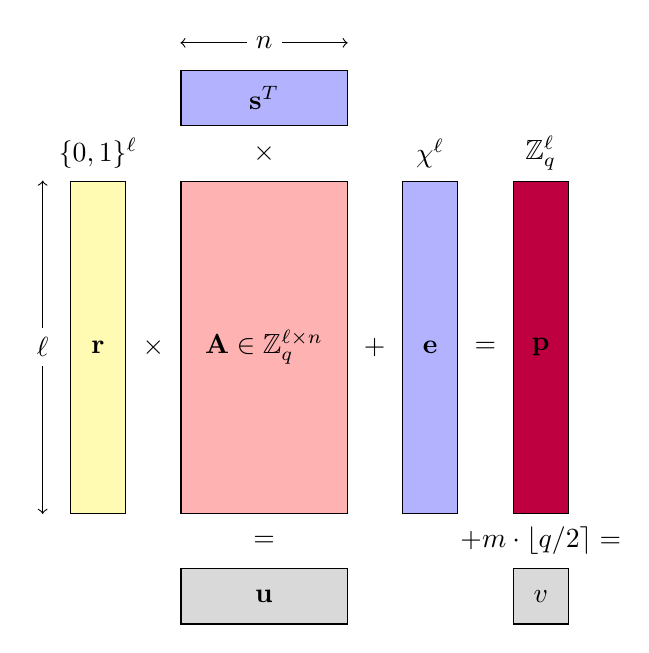
\begin{tikzpicture}
\node[rectanglenode, name=A, minimum width=6em, minimum height=12em, fill=red!30] {$\mathbf{A} \in \mathbb{Z}_q^{\ell \times n}$}; 

\node[textnode, name=product1, left of = A, xshift=-4em] {$\times$}; 
\node[rectanglenode, name=r, left of = product1, xshift=-2em, 
	minimum width=2em, minimum height=12em, fill=yellow!30] {$\mathbf{r}$};
\node[textnode, above of = r, yshift=7em] {$\{0,1\}^\ell$};
\draw ($(r.south)+(-2em, 0em)$) edge[<->] node[fill=white] {$\ell$} ($(r.north)+(-2em, 0em)$); 

\node[textnode, name=product2, above of = A, yshift=7em] {$\times$}; 
\node[rectanglenode, name=sk, above of = product2, yshift=2em, 
	minimum width=6em, minimum height=2em, fill=blue!30] {$\mathbf{s}^T$}; 
\draw ($(sk.west)+(0em, 2em)$) edge[<->] node[fill=white] {$n$} ($(sk.east)+(0em, 2em)$); 

\node[textnode, name=add1, right of = A, xshift=4em] {$+$}; 
\node[rectanglenode, name=e, right of = add1, xshift=2em, 
	minimum width=2em, minimum height=12em, fill=blue!30] {$\mathbf{e}$}; 
\node[textnode, above of = e, yshift=7em] {$\chi^\ell$};

\node[textnode, name=get1, right of = e, xshift=2em] {$=$}; 
\node[rectanglenode, name=pk, right of = get1, xshift=2em, 
	minimum width=2em, minimum height=12em, fill=purple] {$\mathbf{p}$}; 
\node[textnode, above of = pk, yshift=7em] {$\mathbb{Z}_q^\ell$};

\node[textnode, name=get2, below of = A, yshift=-7em] {$=$}; 
\node[rectanglenode, name=u, below of = get2, yshift=-2em, 
	minimum width=6em, minimum height=2em, fill=gray!30] {$\mathbf{u}$}; 

\node[textnode, name=get3, below of = pk, yshift=-7em] {$+ m \cdot \lfloor q/2 \rceil = $}; 
\node[rectanglenode, name=v, below of = get3, yshift=-2em, 
	minimum width=2em, minimum height=2em, fill=gray!30] {$v$}; 
\end{tikzpicture}
\end{center}
\caption{Regev PKE加密方案示意图}
\end{figure}

\begin{theorem}
如果判定性LWE假设成立, 则Regev PKE是IND-CPA安全的. 
\end{theorem}

\begin{proof}
令$S_i$表示敌手在$\text{Game}_i$中成功概率. 以游戏序列的方式组织证明如下:
\begin{trivlist}
\item $\text{Game}_0$: 该游戏是标准的IND-CPA游戏. 
	挑战者$\mathcal{CH}$和敌手$\mathcal{A}$交互如下: 
	\begin{itemize}
		\item 初始化: $\mathcal{CH}$运行$\mathsf{Setup}(1^\kappa)$生成公开参数$\mathbf{A} \in \mathbb{Z}_q^{\ell \times n}$, 
			同时生成公私钥对, 其中私钥$sk$为随机向量$\mathbf{s} \in \mathbb{Z}_q^n$, 
			公钥$pk$为$\mathbf{p} = \mathbf{A}\mathbf{s}+\mathbf{e} \in \mathbb{Z}_q^\ell$, 
			其中$\mathbf{e} \leftarrow \chi^\ell$.  

		\item 挑战: $\mathcal{A}$选取$(m_0, m_1)$发送给$\mathcal{CH}$. 
			$\mathcal{CH}$随机选取$\mathbf{r} \sample \{0,1\}^\ell$, $\beta \sample \{0,1\}$,  
			计算$\mathbf{u} = \mathbf{r}^T \mathbf{A}$, 
			$v = \mathbf{r}^T \mathbf{p} + m_\beta \cdot \lfloor q/2 \rceil$, 
			发送$(\mathbf{u}, v)$给$\mathcal{A}$作为挑战密文. 

		\item 猜测: $\mathcal{A}$输出对$\beta$的猜测$\beta'$. $\mathcal{A}$成功当且仅当$\beta = \beta'$. 
	\end{itemize} 
根据定义, 我们有: 
\begin{equation*}
\AdvA(\kappa) = |\Pr[S_0] - 1/2|
\end{equation*}  

\item $\text{Game}_1$: 与$\text{Game}_0$惟一不同的是$\mathcal{CH}$生成公钥的方式由
	计算$\mathbf{A}\mathbf{s}+\mathbf{e}$变为随机选取$\mathbb{Z}_q^\ell$上的向量. 
	在$\text{Game}_1$中, $\vec{\mathbf{A}} = \mathbf{A} \mid \mathbf{p}$是$\mathbb{Z}_q^{\ell \times n}$上的随机矩阵, 
	容易验证$f_{\vec{\mathbf{A}}}(\mathbf{r}) = \mathbf{r}^T \vec{\mathbf{A}}$是从$\{0,1\}^\ell$到$\mathbb{Z}_q^{n+1}$
	的universal hash, 由参数选取$\ell > n \log q$和剩余哈希引理(leftover hash lemma)可知, 
	函数的输出服从$\mathbb{Z}_q^{n+1}$上的均匀分布. 因此, 挑战密文完美掩盖了$\beta$的信息. 
	因此, 即使对于拥有无穷计算能力的敌手, 我们也有: 
\begin{equation*}
\AdvA(\kappa) = |\Pr[S_1] - 1/2| = 0
\end{equation*} 
\end{trivlist}

\begin{claim}
如果判定性LWE假设成立, 那么对于任意PPT敌手均有$|\Pr[S_0] - \Pr[S_1]| \leq \mathsf{negl}(\kappa)$. 
\end{claim}

\begin{proof}
证明的思路是反证. 若存在PPT敌手$\mathcal{A}$在$\text{Game}_0$和$\text{Game}_1$中成功的概率差不可忽略, 
则可构造出PPT算法$\mathcal{B}$打破LWE困难问题. 令$\mathcal{B}$的LWE挑战实例为$(\mathbf{A}, \mathbf{p})$, 
$\mathcal{B}$的目标是区分挑战实例是随机采样还是LWE采样. 为此$\mathcal{B}$扮演IND-CPA游戏中的挑战者与$\mathcal{A}$交互如下: 
\begin{itemize}
	\item 初始化: $\mathcal{B}$发送$(\mathbf{A}, \mathbf{p})$给$\mathcal{A}$. 
		该操作将$pk$隐式地设定为$\mathbf{p}$. 

	\item 挑战: $\mathcal{A}$选取$(m_0, m_1)$发送给$\mathcal{CH}$. 
		$\mathcal{CH}$随机选取$\mathbf{r} \sample \{0,1\}^\ell$, $\beta \sample \{0,1\}$,  
		计算$\mathbf{u} = \mathbf{r}^T \mathbf{A}$, 
		$v = \mathbf{r}^T \mathbf{p} + m_\beta \cdot \lfloor q/2 \rceil$, 
		发送$(\mathbf{u}, v)$给$\mathcal{A}$作为挑战密文. 

	\item 猜测: $\mathcal{A}$输出对$\beta$的猜测$\beta'$. 如果$\beta = \beta'$, $\mathcal{B}$输出1. 
\end{itemize} 
对上述交互分析可知, 如果$\mathbf{p}$是LWE采样, 那么$\mathcal{B}$完美模拟了$\text{Game}_0$; 
如果$\mathbf{p}$是随机采样, 那么$\mathcal{B}$完美模拟了$\text{Game}_1$. 
因此, $\mathcal{B}$解决LWE挑战的优势$\mathsf{Adv}_\mathcal{B}^\text{LWE}(\kappa) = |\Pr[S_0] - \Pr[S_1]|$. 
如果LWE假设成立, 我们有$|\Pr[S_0] - \Pr[S_1]| \leq \mathsf{negl}(\kappa)$. \qed
\end{proof}
综上, 定理得证. \qed
\end{proof}

\begin{remark}
Regev PKE和Goldwasser-Micali PKE在设计上有异曲同工之处, 均采用的是有损加密思想, 即公钥存在正常和有损这两种计算不可区分的类型, 
正常公钥生成的密文可以正确解密, 而有损公钥生成的密文丢失了明文的全部信息. 
在安全性证明时, 利用两种类型公钥的计算不可区分性以及有损加密的性质, 即可完成IND-CPA安全的论证.   
\end{remark}

\subsection{GPV PKE}
Gentry, Peikert和Vaikuntanathan~\cite{GPV-STOC-2008}同样基于LWE假设设计出一个PKE方案, 称为GPV PKE. 

\begin{trivlist}
\item GPV PKE由以下4个多项式时间算法组成: 
\begin{itemize}
\item $\mathsf{Setup}(1^\kappa)$: 以安全参数$\kappa$为输入, 生成随机矩阵$\mathbf{A} \in \mathbb{Z}_q^{\ell \times n}$作为公开参数. 

\item $\mathsf{KeyGen}(pp)$: 以公开参数$pp$为输入, 随机选取噪声向量$\mathbf{r} \sample D_{\mathbb{Z}^\ell, r}$作为私钥, 
    计算$\mathbf{u}^T \leftarrow \mathbf{r}^T\mathbf{A}$作为公钥. 从编码的角度, $\mathbf{u}$可以理解为$\mathsf{e}$
    相对于$\mathbf{A}$的syndrome. 

\item $\mathsf{Encrypt}(pk, m)$: 以公钥$pk = \mathbf{u}$和明文$m \in \{0,1\}$为输入, 
	随机选取向量$\mathbf{s} \sample \mathbb{Z}_q^n$和$\mathbf{e} \sample \chi^\ell$, 随机选取$e \sample \chi$, 
	计算$\mathbf{p} = \mathbf{A}\mathbf{s}+\mathbf{e} \in \mathbb{Z}_q^\ell$, 
	$v = \mathbf{u}^T \mathbf{s} + e + m \cdot \lfloor q/2 \rceil$作为密文. 

\item $\mathsf{Decrypt}(\mathbf{r}, c)$: 以私钥$sk = \mathbf{r}$和密文$c = (\mathbf{p}, v)$, 
    计算$y = v - \mathbf{r}^T\mathbf{p} \in \mathbb{Z}_q$, 若$y$接近0则输出0, 
    若$y$接近$\lfloor q/2 \rceil$则输出1.    
\end{itemize}
\end{trivlist}

\begin{trivlist}
\item \textbf{正确性.} 观察以下等式: 
\begin{eqnarray*}
y &=& v - \mathbf{r}^T\mathbf{p}\\
  &=& \mathbf{u}^T \mathbf{s} + e + m \cdot \lfloor q/2 \rceil - \mathbf{r}^T(\mathbf{A}\mathbf{s}+\mathbf{e})\\
  &=& \mathbf{u}^T \mathbf{s} + e + m \cdot \lfloor q/2 \rceil - \mathbf{u}^T\mathbf{s} - \mathbf{r}^T\mathbf{e}\\
  &=& m \cdot \lfloor q/2 \rceil + e - \mathbf{r}^T\mathbf{e}
\end{eqnarray*}
由上述推导可知, 当累计误差$|\langle e - \mathbf{r}^T\mathbf{e} \rangle|\leq q/4$时解密正确. 
通过恰当的参数选择, 可确保累计误差以接近1的绝对优势概率小于等于$q/4$, 更多细节请参考~\cite{GPV-STOC-2008}
\end{trivlist}

\begin{figure}
\begin{center}
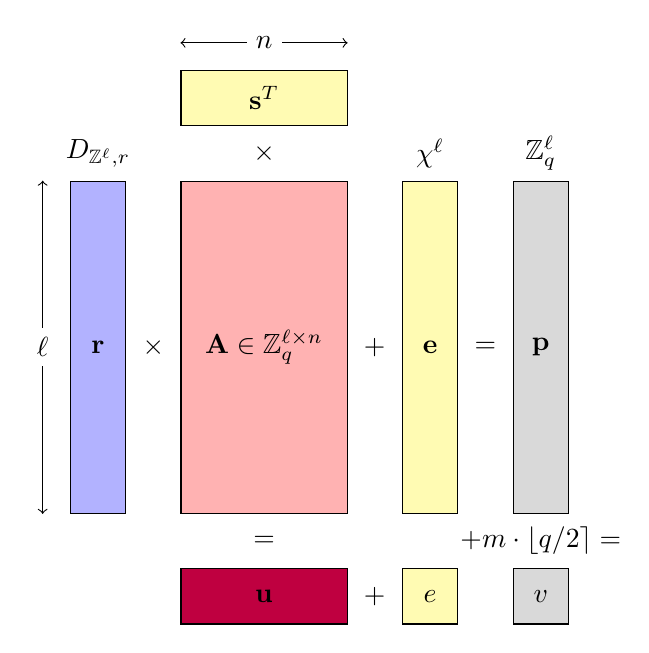
\begin{tikzpicture}
\node[rectanglenode, name=A, minimum width=6em, minimum height=12em, fill=red!30] {$\mathbf{A} \in \mathbb{Z}_q^{\ell \times n}$}; 

\node[textnode, name=product1, left of = A, xshift=-4em] {$\times$}; 
\node[rectanglenode, name=r, left of = product1, xshift=-2em, 
	minimum width=2em, minimum height=12em, fill=blue!30] {$\mathbf{r}$};
\node[textnode, above of = r, yshift=7em] {$D_{\mathbb{Z}^\ell, r}$};
\draw ($(r.south)+(-2em, 0em)$) edge[<->] node[fill=white] {$\ell$} ($(r.north)+(-2em, 0em)$); 

\node[textnode, name=product2, above of = A, yshift=7em] {$\times$}; 
\node[rectanglenode, name=sk, above of = product2, yshift=2em, 
	minimum width=6em, minimum height=2em, fill=yellow!30] {$\mathbf{s}^T$}; 
\draw ($(sk.west)+(0em, 2em)$) edge[<->] node[fill=white] {$n$} ($(sk.east)+(0em, 2em)$); 

\node[textnode, name=add1, right of = A, xshift=4em] {$+$}; 
\node[rectanglenode, name=e, right of = add1, xshift=2em, 
	minimum width=2em, minimum height=12em, fill=yellow!30] {$\mathbf{e}$}; 
\node[textnode, above of = e, yshift=7em] {$\chi^\ell$};

\node[textnode, name=get1, right of = e, xshift=2em] {$=$}; 
\node[rectanglenode, name=pk, right of = get1, xshift=2em, 
	minimum width=2em, minimum height=12em, fill=gray!30] {$\mathbf{p}$}; 
\node[textnode, above of = pk, yshift=7em] {$\mathbb{Z}_q^\ell$};

\node[textnode, name=get2, below of = A, yshift=-7em] {$=$}; 
\node[rectanglenode, name=u, below of = get2, yshift=-2em, 
	minimum width=6em, minimum height=2em, fill=purple] {$\mathbf{u}$}; 

\node[textnode, name=add2, right of = u, xshift=4em] {$+$}; 
\node[rectanglenode, name=e_star, right of = add2, xshift=2em, 
	minimum width=2em, minimum height=2em, fill=yellow!30] {$e$}; 

\node[textnode, name=get3, below of = pk, yshift=-7em] {$+ m \cdot \lfloor q/2 \rceil = $}; 
\node[rectanglenode, name=v, below of = get3, yshift=-2em, 
	minimum width=2em, minimum height=2em, fill=gray!30] {$v$}; 
\end{tikzpicture}
\end{center}
\caption{GPV PKE加密方案示意图}
\end{figure}

\begin{theorem}
如果判定性LWE假设成立, 则GPV PKE是IND-CPA安全的. 
\end{theorem}

\begin{proof}
令$S_i$表示敌手在$\text{Game}_i$中成功概率. 以游戏序列的方式组织证明如下:
\begin{trivlist}
\item $\text{Game}_0$: 该游戏是标准的IND-CPA游戏. 
	挑战者$\mathcal{CH}$和敌手$\mathcal{A}$交互如下: 
	\begin{itemize}
		\item 初始化: $\mathcal{CH}$运行$\mathsf{Setup}(1^\kappa)$生成公开参数$\mathbf{A} \in \mathbb{Z}_q^{\ell \times n}$, 
			同时生成公私钥对, 其中私钥$sk$为随机向量$\mathbf{r} \in D_{\mathbb{Z}^\ell, r}$, 
			公钥$pk$为$\mathbf{u} = \mathbf{r}^T\mathbf{A}$.  

		\item 挑战: $\mathcal{A}$选取$(m_0, m_1)$发送给$\mathcal{CH}$. 
			$\mathcal{CH}$随机选取$\mathbf{s} \sample \mathbb{Z}_q^n$, 
			随机选取$\mathbf{e} \sample \chi^\ell$和$e \sample \chi$, $\beta \sample \{0,1\}$,  
			计算$\mathbf{p} = \mathbf{A}\mathbf{s}+\mathbf{e} \in \mathbb{Z}_q^\ell$, 
			$v = \mathbf{u}^T \mathbf{s} + e + m_\beta \cdot \lfloor q/2 \rceil$作为密文. 
			发送$(\mathbf{u}, v)$给$\mathcal{A}$作为挑战密文. 

		\item 猜测: $\mathcal{A}$输出对$\beta$的猜测$\beta'$. $\mathcal{A}$成功当且仅当$\beta = \beta'$. 
	\end{itemize} 
根据定义, 我们有: 
\begin{equation*}
\AdvA(\kappa) = |\Pr[S_0] - 1/2|
\end{equation*}  

\item $\text{Game}_1$: 与$\text{Game}_0$惟一不同的是$\mathcal{CH}$生成公钥的方式由
	计算$\mathbf{u}^T = \mathbf{r}^T \mathbf{A}$变为随机选取$\mathbf{u} \sample \mathbb{Z}_q^n$上的向量. 
	在$\text{Game}_1$中, $(\mathbf{A}, \mathbf{p} = \mathbf{A}\mathbf{s}+\mathbf{e}, \mathbf{u}, \mathbf{u}^T\mathbf{s}+x)$
	恰好构成$\ell+1$个LWE采样结果. 有LWE假设立刻可知, 敌手在$\text{Game}_1$中的视角计算意义下隐藏了$\beta$的信息, 
	因此基于LWE假设有: 
\begin{equation*}
\AdvA(\kappa) = |\Pr[S_1] - 1/2| \leq \mathsf{negl}(\kappa)
\end{equation*}
\end{trivlist} 

\begin{claim}
对于任意的敌手$\mathcal{A}$(即使拥有无穷计算能力), 均有$|\Pr[S_0] - \Pr[S_1]| \leq \mathsf{negl}(\kappa)$ 
\end{claim}

\begin{proof}
根据$\ell \geq 2n \log q$的参数选择可知, 公钥$\mathbf{u}$的分布与$\mathbb{Z}_q^n$上的均匀分布统计不可区分, 
因此敌手在$\text{Game}_0$和$\text{Game}_1$中的视图统计不可区分, 
从而$|\Pr[S_0] - \Pr[S_1]| \leq \mathsf{negl}(\kappa)$. \qed
\end{proof}

综上, 定理得证. \qed
\end{proof}

\begin{remark}
Regev PKE和GPV PKE在形式上相似, 构造使用了相同的元素$\mathbf{A}, \mathbf{s}, \mathbf{r}, \mathbf{e}, \mathbf{p}, \mathbf{u}, v$, 
但用途含义不完全相同, 构造互为对偶. Regev PKE中, $\mathbf{p}$为公钥, $(\mathbf{s}, \mathbf{e})$为私钥, $\mathbf{u}$为密文; 
GPV PKE中$\mathbf{p}$为密文, $(\mathbf{s}, \mathbf{e})$为加密随机数, $\mathbf{u}$为公钥. 
感兴趣的读者可以参考Micciancio~\cite{Micciancio-PKC-2010}了解更多格密码学中的对偶性. 
Regev PKE中, 公钥空间是稀疏的; GPV PKE中, 公钥空间是稠密的, 正是利用公钥空间的稠密性, 
我们可以借助随机谕言机将GPV PKE升级为身份加密方案GPV IBE. 
\end{remark}

\chapter{通用构造方法}
\begin{introduction}
  \item 单向陷门函数类
  \item 哈希证明系统类
  \item 可提取哈希证明系统类
  \item 程序混淆类
  \item 统一构造框架
\end{introduction}
\section{单向陷门函数类}

\subsection{单向陷门函数}
单向陷门函数(TDF)是单向函数(OWF)在Cryptomania中的对应, 简言之, 其正向计算容易, 逆向计算困难但在有陷门信息辅助时同样容易. 
\begin{definition}[单向陷门函数]
TDF由以下四个多项式时间算法组成: 
\begin{itemize}
\item $\mathsf{Setup}(1^\kappa)$: 系统生成算法以安全参数$\kappa$为输入, 输出公开参数$pp$, 
	其中$pp$包含对定义域$D$, 值域$R$, 求值公钥空间$EK$、求逆陷门空间$TD$和单向陷门函数族
	$f: EK \times D \rightarrow R$的描述. 换言之, $f$是由求值公钥索引的函数族.  
	不失一般性, $D$支持高效的随机采样, 即存在PPT算法$\mathsf{SampDom}$可以从$D$中随机选取一个元素.   
	在多数情况下, $D$和$R$是与求值公钥无关的(该性质也被称为index-independent), 
	但在有些情形下, $D$和$R$是由求值公钥索引的空间簇. 
	为了叙述简洁, 以下均假设$D$和$R$是单一空间. 空间簇的情形由单一集合的情形自然推广得到.   

\item $\mathsf{KeyGen}(pp)$: 以公共参数$pp$为输入, 输出密钥对$(ek, td)$, 
	其中$ek$为求值公钥, $td$为求逆陷门. 

\item $\mathsf{Eval}(ek, x)$: 以求值公钥$ek$和定义域元素$x \in D$为输入, 输出$y \leftarrow f_{ek}(x)$.  

\item $\mathsf{TdInv}(td, y)$: 以求逆陷门$td$和值域元素$y \in R$为输入, 输出$x \in D$或特殊符号$\bot$指示$y$不存在原像.       
\end{itemize}
\end{definition}

定义以下两条性质: 
\begin{itemize}
\item 单射: $\forall ek$, 称$f_{ek}$是单射的当且仅当$x \neq x' \Rightarrow f_ek(x) \neq f_{ek}(x')$. 
\item 置换: $\forall ek$, $\text{Img}(f_ek) = D = R$.
\end{itemize}

\begin{center}
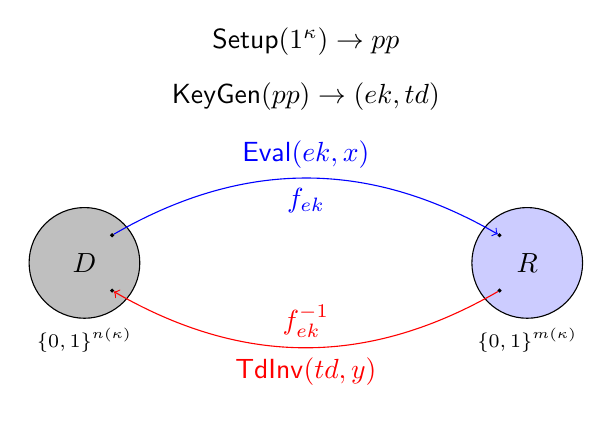
\begin{tikzpicture}
    \node [name=Setup, textnode] {$\mathsf{Setup}(1^\kappa) \rightarrow pp$}; 
    \node [name=KeyGen, textnode, below of = Setup, yshift=-2em] {$\mathsf{KeyGen}(pp) \rightarrow (ek, td)$}; 

    \node [name=domain, circlenode, fill=gray!50, minimum size=4em, 
        below of = KeyGen, yshift=-6em, xshift=-8em, label=below:\scriptsize{$\{0,1\}^{n(\kappa)}$}] {$D$}; 
    \node [name=range, circlenode, fill=blue!20, minimum size=4em, 
        below of = KeyGen, yshift=-6em, xshift=8em, label=below:\scriptsize{$\{0,1\}^{m(\kappa)}$}] {$R$}; 

    \node [name=x1, circlenode, fill=black, right of = domain, xshift=1em, yshift=1em, 
        minimum size=0.1em, inner sep=0em] {};
    \node [name=y1, circlenode, fill=black, left of = range, xshift=-1em, yshift=1em, 
        minimum size=0.1em, inner sep=0em] {}; 
    \draw (x1) edge[->, color=blue, bend left=30] node[above] {$\mathsf{Eval}(ek, x)$} node[below] {$f_{ek}$} (y1);

    \node [name=x2, circlenode, fill=black, right of = domain, xshift=1em, yshift=-1em, 
        minimum size=0.1em, inner sep=0em] {};
    \node [name=y2, circlenode, fill=black, left of = range, xshift=-1em, yshift=-1em, 
        minimum size=0.1em, inner sep=0em] {}; 
    \draw (y2) edge[->, color=red, bend left=30] node[above] {$f_{ek}^{-1}$} node[below] {$\mathsf{TdInv}(td, y)$} (x2);
\end{tikzpicture}
\end{center}

\begin{trivlist}
\item \textbf{正确性.} $\forall \kappa \in \mathbb{N}$, $\forall pp \leftarrow \mathsf{Setup}(1^\kappa)$, 
	$\forall (ek, td) \leftarrow \mathsf{KeyGen}(pp)$和$\forall x \in D$和$y = \mathsf{Eval}(ek, x)$, 有: 
	\begin{equation*}
		\Pr[\mathsf{TdInv}(td, y) \in f_{ek}^{-1}(y)] = 1
	\end{equation*}
\end{trivlist}

\begin{trivlist}
\item \textbf{单向性.} 定义单向陷门函数敌手$\mathcal{A}$的优势函数如下:
\begin{displaymath}
	\AdvA(\kappa) =
		\Pr \left[ x \in f_{ek}^{-1}(y^*): 
			\begin{array}{ll}
         		& pp \leftarrow \mathsf{Setup}(1^\kappa);\\
				& (ek, td) \leftarrow \mathsf{KeyGen}(pp);\\
         		& x^* \sample D, y^* \leftarrow \mathsf{Eval}(ek, x^*);\\
         		& x \leftarrow \mathcal{A}(pp, ek, y^*)
			\end{array} 
		\right],
\end{displaymath}	 
如果对于任意的PPT敌手$\mathcal{A}$, 其优势函数均是可忽略的, 则称该陷门函数是单向的. 
\end{trivlist}

\begin{remark}
\begin{enumerate}
\item 不失一般性, 假定$D$和$R$均存在经典表示, 分别是$\{0,1\}^{n(\kappa)}$和$\{0,1\}^{m(\kappa)}$, 
	其中$n(\cdot)$和$m(\cdot)$是关于$\kappa$的多项式函数. 
	容易验证, 长度函数不能过大, 如果$n(\cdot)$或$m(\cdot)$是超多项式函数, 则函数无法高效计算; 
	长度函数也不能过小, 如果$n(\cdot)$或$m(\cdot)$是亚线性函数, 则函数不可能满足单向性. 

\item 在抽象定义中, 只限定了$\mathsf{TDFInv}(td, \cdot)$在输入为像集元素时返回原像, 而未限定其输入为非像集元素时的行为. 
	在具体构造时, $\mathsf{TDFInv}(td, \cdot)$在输入为非像集元素时的行为往往需要精心设定, 以方便安全性证明. 

\item 在单向性的定义中, 敌手$\mathcal{A}$仅观察到$ek$和$y^*$的信息. 
	$x^* \sample D$可以放宽至$x^*$选自$D$上的高最小熵分布, 即$\mathsf{H}_{\infty}(x^*) \geq \omega(\log \kappa)$.
\end{enumerate}
\end{remark}

在展示如何使用单向陷门函数构造公钥方案之前, 先展示一个基于单向陷门置换的构造. 该构造并不安全, 但对得到正确的构造很有启发意义. 

\begin{construction}[朴素的TDF-based PKE(不安全)]
\begin{itemize}
\item $\mathsf{Setup}(1^\kappa)$: 运行$\text{TDP}.\mathsf{Setup}(1^\kappa)$生成公开参数$pp$, 
	其中明文空间和密文空间均为单向陷门置换的定义域$D$. 

\item $\mathsf{KeyGen}(pp)$: 运行$\text{TDP}.\mathsf{KeyGen}(pp) \rightarrow (ek, td)$, 
	其中$ek$作为加密公钥, $td$作为解密私钥. 

\item $\mathsf{Encrypt}(ek, m)$: 以公钥$ek$和明文$m \in D$为输入, 运行$\text{TDP}.\mathsf{Eval}(ek, m)$
	计算$c \leftarrow f_{ek}(m)$作为密文.  

\item $\mathsf{Decrypt}(td, c)$: 以私钥$td$和密文$c \in D$为输入, 运行$\text{TDP}.\mathsf{TdInv}(td, c)$
	计算$m \leftarrow f_{ek}^{-1}(c)$恢复明文. 
\end{itemize}
\end{construction}

上述构造来自Diffie和Hellman的经典论文~\cite{DH-IEEE-IT-1976}, 原始的RSA公钥加密方案就是该构造的具体实例化. 
该构造的想法直观, 利用单向陷门置换将明文转化为密文, 同时利用陷门可以求逆从密文中恢复明文. 
但其仅仅满足较弱的OW-CPA安全, 并不满足现在公认的最低要求IND-CPA安全, 
因此其也被成为公钥加密的textbook构造\footnote{textbook指其仅适合作为以科普为目的教学.}.
朴素构造不满足IND-CPA安全的根本原因是加密算法是确定型的而非概率型的, 因此敌手可以通过``加密-比较''即可打破IND-CPA安全. 
因此, 强化朴素构造的第一步是选择定义域中的随机元素$x$, 计算其函数值$f_{ek}(x)$作为封装密文, 再用$x$作为会话密钥掩蔽明文. 
强化构造仍然不满足IND-CPA安全性, 原因是$f_{ek}(\cdot)$是公开可计算函数, 其函数值泄漏了原像信息, 使得原像在敌手的视角中不再伪随机. 
针对性的强化方法是计算$x$的hardcore function值作为会话密钥. 

以下首先介绍hardcore function的概念. 
\begin{definition}[hardcore function]
称多项式时间可计算的确性型函数$\mathsf{hc}: D \rightarrow K$是函数$f: D \rightarrow R$的hardcore function当且仅当: 
\begin{equation*}
	(f(x^*), \mathsf{hc}(x^*)) \approx_c (f(x^*), U_K) 
\end{equation*} 
其中概率空间建立在$x^* \sample D$的随机带上. 以安全实验的方式可如下定义, 即对于任意PPT敌手$\mathcal{A}$, 其安全优势可忽略: 
\begin{displaymath}
	\AdvA(\kappa) =
		\Pr \left[ \beta'=\beta: 
			\begin{array}{l}
         		pp \leftarrow \mathsf{Setup}(1^\kappa);\\
         		x^* \sample D, y^* \leftarrow f(x^*);\\
         		k_0^* \leftarrow \mathsf{hc}(x^*), k_1^* \sample K, \beta \sample \{0,1\};\\
         		\beta' \leftarrow \mathcal{A}(pp, ek, y^*, k_\beta^*);
			\end{array} 
		\right] - \frac{1}{2}
\end{displaymath}	
\end{definition}  

\begin{center}
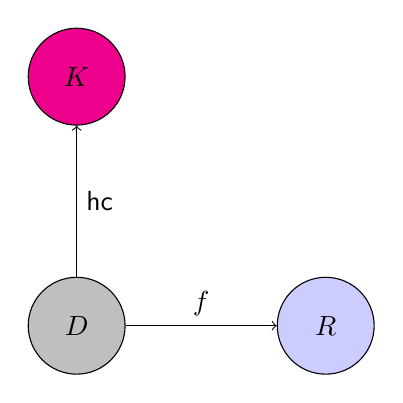
\begin{tikzpicture}
\node [name=domain, circlenode, fill=gray!50, minimum size=3.5em] {$D$}; 
\node [name=range, circlenode, fill=blue!20, minimum size=3.5em, right of = domain, xshift=9em] {$R$}; 
\node [name=K, circlenode, fill=magenta, minimum size=3.5em, above of = domain, yshift=9em] {$K$};
\draw (domain) edge[->] node[auto] {$f$} (range);
\draw (domain) edge[->] node[right] {$\mathsf{hc}$} (K); 
\end{tikzpicture}
\end{center}

\begin{theorem}[Goldreich-Levin Theorem] 
如果$f: \{0,1\}^n \rightarrow \{0,1\}^m$是单向函数, 
那么$\mathsf{GL}(x) = \bigoplus_{i=1}^n x_i r_i$是从$\{0,1\}^n$到$\{0,1\}$的单比特输出硬核函数, 或称为硬核谓词. 
\end{theorem}

\begin{remark}
Goldreich-Levin定理是现代密码学中极为重要的结论, 它的意义在于通过显式构造硬核函数, 建立起单向性与伪随机性之间的关联. 
从另一个角度理解, $\mathsf{GL}$硬核谓词可以看做一个计算意义下的随机性提取器, 
对$x|f(x)$的计算熵进行随机性提取, 萃取出伪随机的一比特. 
还需要特别说明的是, 到目前为止尚不知晓如何针对任意单向函数$f$设计一个确定型的硬核谓词. 
$\mathsf{GL}$是相对于$g(x, r):=f(x)||r$的硬核谓词, 或者可以将$r \sample \{0,1\}^n$理解为硬核谓词的描述, 
将$\mathsf{GL}$理解为$f$的随机性硬核谓词. 
本书中采用第二种观点.  

另一方面, $\mathsf{GL}$硬核谓词是通用的(universal), 即构造对于任意单向函数均成立. 强通用性的代价是效率较低, 输出仅是单比特. 
当单向函数具有特殊的结构(如函数是置换)或者依赖额外困难假设(如判定性假设、差异输入程序混淆假设)时, 存在更高效的构造. 
\end{remark}

以下我们展示如何基于单射的单向陷门函数构造构造KEM方案. 
\begin{construction}[TDF-based KEM]\label{construction:TDF-based-KEM}
\begin{itemize}
\item $\mathsf{Setup}(1^\kappa)$: 运行$\text{TDF}.\mathsf{Setup}(1^\kappa)$生成公开参数$pp$. 
	$pp$中不仅包含单向陷门函数$f_{ek}: D \rightarrow R$的描述, 
	还包括相应硬核函数$\mathsf{hc}: D \rightarrow K$的描述.  
	KEM方案的密文空间是TDF的定义域$D$, 密钥空间是硬核函数的值域$K$. 

\item $\mathsf{KeyGen}(pp)$: 运行$\text{TDF}.\mathsf{KeyGen}(pp) \rightarrow (ek, td)$, 
	其中$ek$作为封装公钥$pk$, $td$作为解封装私钥$sk$. 

\item $\mathsf{Encaps}(pk, m)$: 以公钥$pk=ek$为输入, 随机选取$x \sample D$, 
	运行$\text{TDF}.\mathsf{Eval}(ek, x)$计算$c \leftarrow f_{ek}(m)$作为封装密文, 
	计算$k \leftarrow \mathsf{hc}(x)$作为会话密钥.  

\item $\mathsf{Decaps}(sk, c)$: 以私钥$sk=td$和密文$c$为输入, 运行$\text{TDF}.\mathsf{TdInv}(td, c)$
	计算$x \leftarrow f_{ek}^{-1}(c)$, 输出$k \leftarrow \mathsf{hc}(x)$. 
\end{itemize}
\end{construction}
\begin{trivlist}
\item \textbf{正确性.} 由单向陷门函数的单射性质和求逆算法的正确性可知, 上述KEM构造满足正确性. 
\end{trivlist}

\begin{theorem}
如果$f_{ek}$是一族单射单向陷门函数, 那么上述KEM构造是IND-CPA安全的. 
\end{theorem}

\begin{proof}
证明的思路是单一归约, 即若存在敌手$\mathcal{A}$打破KEM方案的IND-CPA安全性, 
则存在敌手$\mathcal{B}$打破$\mathsf{hc}$的伪随机性, 进而与$f_{ek}$的单向性矛盾. 
令$\mathcal{B}$的挑战实例为$(pp, ek, y^*, k_\beta^*)$, 其中$pp$为单射单向陷门函数的公开参数, 
$ek$为随机生成的求值密钥, $y^* \leftarrow f_{ek}(x^*)$是随机选取原像$x^*$的像, 
$k_0^* \leftarrow \mathsf{hc}(x^*)$, $k_1^* \sample K$
$\mathcal{B}$的目标是判定$\beta=0$抑或$\beta=1$. $\mathcal{B}$与$\mathcal{A}$交互如下: 
\begin{itemize}
\item 初始化: $\mathcal{B}$根据$pp$生成KEM方案的公开参数, 并设定公钥$pk:=ek$, 将$(pp, ek)$发送给$\mathcal{A}$. 
\item 挑战: $\mathcal{B}$设定$c^*:=y^*$, 将$(c^*, k_\beta^*)$发送给$\mathcal{A}$. 
\item 猜测: $\mathcal{A}$输出$\beta'$, $\mathcal{B}$将$\beta'$转发给它自身的挑战者.
\end{itemize}
容易验证, $\mathcal{B}$完美地模拟了KEM方案中的挑战者, $\mathcal{B}$成功当且仅当$\mathcal{A}$成功. 因此我们有: 
\begin{equation*}
\AdvA^\text{KEM}(\kappa) = \AdvB^\text{hc}(\kappa)
\end{equation*}
由$f_{ek}$的单向性可知, $\mathsf{hc}$伪随机, 从KEM构造满足IND-CPA安全性. \qed
\end{proof}

以上的结果展示了单射单向陷门函数蕴含IND-CPA的公钥加密. \blue{需要确认TDF与CCA PKE之间是否存在分离}
一个自然的问题是, 单向陷门函数需要满足何种性质才能蕴含IND-CCA的公钥加密. 
以下, 我们按照时间先后顺序依次介绍单向陷门函数的三个增强版本, 并展示如何基于这些增强版本的单向陷门函数构造IND-CCA的公钥加密. 

\subsection{有损陷门函数}
\begin{center}
    天之道, 损有余而补不足, 是故虚胜实, 不足胜有余. \\
                \hfill --- 宋 $\cdot$ 黄裳《九阴真经》
\end{center}

理想世界中的镜中月和水中花体现的是信息完美复刻, 而现实世界中更多的现象体现的却是信息有损, 如拍照、录音, 无论设备和手段多么先进, 
都无法做到完美复刻信源信息, 只能做到尽可能的高保真. 
单射函数可以形象的理解为理想世界中信息无损的编码过程, 那么什么形式的函数刻画了现实世界中信息有损的编码过程呢? 
Peikert和Waters~\cite{PW-STOC-2008}正是基于上述的思考, 在2008年开创性提出了有损陷门函数的概念. 
简言之, 有损陷门函数有两种模式, 即正常和有损模式. 
在单射模式下, 函数是单射的, 像完全保留了原像的全部信息; 
在有损模式下, 函数是有损的, 像在信息论意义下丢失了原像的部分信息. 两种模式之间的关联是计算不可区分. 

\begin{definition}[有损陷门函数LTDF]
有损陷门函数LTDF由$n$和$\tau$两个参数刻画, 包含以下五个多项式时间算法: 
\begin{itemize}
\item $\mathsf{Setup}(1^\kappa)$: 系统生成算法以安全参数$\kappa$为输入, 输出公开参数$pp$, 
	其中$pp$包含对定义域$X$和值域$Y$的描述. 其中$|X| = 2^{n(\kappa)}$.  

\item $\mathsf{GenInjective}(pp)$: 以公共参数$pp$为输入, 输出密钥对$(ek, td)$, 其中$ek$为求值公钥, $td$为求逆陷门. 
	该算法输出的$ek$定义了从$X$到$Y$的单射函数$f_{ek}$, 拥有对应$td$可以对$f_{ek}$进行高效求逆.  

\item $\mathsf{GenLossy}(pp)$: 以公共参数$pp$为输入, 输出密钥对$(ek, \bot)$, 
	其中$ek$为求值公钥, $\bot$表示陷门不存在无法求逆. 
	该算法输出的$ek$定义了从$D$到$R$的有损函数$f_{ek}$, 像集的大小至多为$2^{\tau(\kappa)}$.  

\item $\mathsf{Eval}(ek, x)$: 以求值公钥$ek$和定义域元素$x \in X$为输入, 输出$y \leftarrow f_{ek}(x)$.  

\item $\mathsf{TdInv}(td, y)$: 以求逆陷门$td$和值域元素$y \in Y$为输入, 输出$x \in X$或特殊符号$\bot$指示$y$不存在原像.       
\end{itemize}

\begin{trivlist}
\item \textbf{模式不可区分性.} $\mathsf{GenInjective}(pp)$和$\mathsf{GenLossy}(pp)$的第一个输出构成的分布在计算意义下不可区分, 
	即任意PPT敌手无法判定求值公钥$ek$属于单射模式还是有损模式. 
\end{trivlist}
\end{definition}

\begin{figure}[!hbtp]
\begin{center}
\begin{tikzpicture}
\node [textnode, name=injective] {单射模式\\$\mathsf{GenInjective}(pp) \rightarrow (ek, td)$}; 
\node [shapenode, name=domain1, circle, draw=gray!50, fill=gray!50, minimum size=4em, right of = injective, xshift=12em] {$X$}; 
\node [shapenode, name=range1, circle, draw=blue!20, fill=blue!20, minimum size=4em, right of = domain1, xshift=12em] {$Y$}; 
\node [shapenode, name=x, circle, draw=black, fill=black, right of = domain1, inner sep =0, minimum size=0.1em, xshift=1em] {};
\node [shapenode, name=y, circle, draw=black, fill=black, left of = range1, inner sep = 0, minimum size=0.1em, xshift=-1em] {}; 
\draw (x) edge[->] node[auto] {$f_{ek}$} (y);
\draw (y) edge[->, bend left=-45, red] node[above] {$f_{ek}^{-1}$} (x);

\node [name=indistinguishable, below of=injective, yshift=-1em] {$\approx_c$};

\draw ($(indistinguishable.east)+(4em, 0em)$) edge[dashed] ($(indistinguishable.east)+(22em, 0em)$);

\node [textnode, name = lossy, below of=indistinguishable, yshift=-4em] 
    {$\mathsf{GenLossy}(pp) \rightarrow (ek, \bot)$\\有损模式};  
\node [shapenode, name=domain2, circle, draw=gray!50, fill=gray!50, minimum size=4em, 
    right of = lossy, xshift=12em] {$X$}; 
\node [shapenode, name=range2, circle, draw=blue!20, fill=blue!20, minimum size=4em, 
    right of = domain2, xshift=12em] {\quad$Y$}; 
\node [shapenode, name=image, circle, draw=blue!60, fill=blue!60, minimum size=1em, left of = range2, xshift=-1em] {}; 

\node [shapenode, draw=black, circle, fill=black, name=xlossy, right of = domain2, 
    inner sep=0, minimum size=0.1em, xshift=1em] {};
\node [shapenode, draw=black, circle, fill=black, name=ylossy, left of = range2, 
    inner sep=0, minimum size=0.1em, xshift=-1em] {}; 
\draw (xlossy) edge[connect] node[auto] {$f_{ek}$} (ylossy);

\node [shapenode, draw=black, circle, fill=black, name=x1, right of = domain2, inner sep = 0, 
    minimum size=0.1em, xshift=0.4em, yshift=1.5em] {};
\node [shapenode, draw=black, circle, fill=black, name=x2, right of = domain2, inner sep = 0, 
    minimum size=0.1em, xshift=0.8em, yshift=0.75em] {};

\node [shapenode, draw=black, circle, fill=black, name=x3, right of = domain2, inner sep = 0, 
    minimum size=0.1em, xshift=0.8em, yshift=-0.75em] {};
\node [shapenode, draw=black, circle, fill=black, name=x4, right of = domain2, inner sep = 0,  
    minimum size=0.1em, xshift=0.4em, yshift=-1.5em] {};

\draw (x1) edge[-, bend left=45] (ylossy);
\draw (x2) edge[-, bend left=30] (ylossy);
\draw (x3) edge[-, bend left=-30] (ylossy);
\draw (x4) edge[-, bend left=-45] (ylossy);

\node [textnode, name=domainsize, below of = domain2, yshift=-4em] {$2^n$}; 
\node [textnode, right of = domainsize, xshift=6em] {$\gg$}; 
\node [textnode, name=imagesize, below of = image, yshift=-4em] {$2^{\tau}$};
\end{tikzpicture}
\end{center}
\caption{有损陷门函数(LTDF)示意图}
\end{figure}

相比常规的单向陷门函数, 有损陷门函数额外具备一个计算不可区分的有损模式, 这正是其威力的来源. 
在利用有损陷门函数设计密码方案/协议时, 通常按照如下的步骤:
\begin{enumerate}
	\item 在单射模式下完成密码方案/协议的功能性构造(功能性通常需要函数单射可逆)
	\item 在有损模式下完成密码方案/协议的安全性论证(论证通常在信息论意义下进行)
	\item 利用单射模式和有损模式的计算不可区分性证明密码方案/协议在正常模式下计算安全性. 
\end{enumerate} 

细心的读者可能已经发现了有损陷门函数的定义中并没有显式的要求函数在单射模式下具备单向性, 
这是因为单射和有损模式的计算不可区分性已经隐式的保证了这一点. 以下进行严格证明, 具体展示应用有损陷门函数设计密码方案/协议的过程. 

\begin{theorem}
令$\mathcal{F}$是一族$(n, \tau)$-LTDF, 当$n - \tau \geq \omega(\log \lambda)$时, 
$\mathcal{F}$的单射模式构成一族单射单向陷门函数.  
\end{theorem}

\begin{proof}
证明通过游戏序列组织. 
\begin{trivlist}
\item $\text{Game}_0$: 该游戏是标准的单射单向陷门函数安全游戏. 挑战者$\mathcal{CH}$和敌手$\mathcal{A}$交互如下:
\begin{itemize}
\item 初始化: $\mathcal{CH}$运行$pp \leftarrow \mathsf{Setup}(\kappa)$, 
    $(ek, td) \leftarrow \mathsf{GenInjective}(pp)$, 发送$(pp, ek)$给$\mathcal{A}$. 

\item 挑战阶段: $\mathcal{CH}$随机选择$x^* \sample X$, sends $y^* \leftarrow f_{ek}(x^*)$给$\mathcal{A}$. 
    
\item 猜测阶段: $\mathcal{A}$输出$x'$, $\mathcal{A}$赢得游戏当且仅当$x' = x^*$. 
\end{itemize}
根据定义, 我们有: 
\begin{equation*}
	\AdvA(\kappa) = \Pr[S_0]
\end{equation*}

\item $\text{Game}_1$: 该游戏与上一个游戏完全相同, 唯一不同的是将单射模式切换到有损模式 
\begin{itemize}
\item 初始化: $\mathcal{CH}$运行\redul{$(ek, \bot) \leftarrow \mathsf{GenLossy}(pp)$}生成求值公钥$ek$. 
\end{itemize}
根据定义, 我们有: 
\begin{equation*}
	\AdvA(\kappa) = \Pr[S_1]
\end{equation*}
\end{trivlist}

\begin{claim}
单射和有损两种模式的计算不可区分性保证了$|\Pr[S_0] - \Pr[S_1]| \leq \mathsf{negl}(\kappa)$.  
\end{claim}

\begin{proof}
我们利用反证法完成归约论证: 若$|\Pr[S_0] - \Pr[S_1]|$不可忽略, 则可构造出PPT的敌手$\mathcal{B}$打破模式的不可区分性. 
$\mathcal{B}$在收到模式不可区分性的挑战$(pp, ek)$后, 将$(pp, ek)$发送给$\mathcal{A}$, 
随后随机选取$x^* \sample X$, 计算并发送$y^* \leftarrow f_{ek}(x^*)$给$\mathcal{A}$. 
当收到$\mathcal{A}$的输出$x'$后, 若$x' = x^*$, $\mathcal{B}$输出`1', 否则输出`0'. 
分析可知, 当$ek$来自单射模式时, $\mathcal{B}$完美的模拟了$\text{Game}_0$; 
当$ek$来自有损模式时, $\mathcal{B}$完美的模拟了$\text{Game}_1$. 
因此, 我们有: 
\begin{equation*}
|\Pr[\mathcal{B}(ek)=1: ek \leftarrow \mathsf{GenInjective}(pp)] - 
\Pr[\mathcal{B}(ek)=1: ek \leftarrow \mathsf{GenLossy}(pp)]| = |\Pr[S_0] - \Pr[S_1]| 
\end{equation*} 
其中$pp \leftarrow \mathsf{Setup}(1^\kappa)$. \qed
\end{proof}

\begin{claim}
对于任意的敌手$\mathcal{A}$(即使拥有无穷计算能力), 其在$\textup{Game}_1$中的优势也是可忽略的. 
\end{claim}

\begin{proof}
$\textup{Game}_1$处于有损模式, 因此由Chainning Lemma~\ref{lemma:chainning-lemma}可知, $x^*$
的平均条件最小熵$\avminentropy(x^*|y^*) \geq n - \tau \geq \omega(\log \kappa)$, 从而断言得证. \qed
\end{proof}

综合以上, 定理得证! \qed
\end{proof}

\begin{remark}
有损陷门函数相比标准单向陷门函数多了有损模式, 也正因为如此, 其具有标准单向陷门函数很多不具备的优势. 

在安全方面, 根据上述论证容易验证只要参数设置满足一定约束, 则有损(陷门)函数在泄漏模型下仍然安全. 
具体的, 在敌手获得关于原像任意长度为$\ell$有界泄漏的情形下, 
只要$n - \tau - \ell \geq \omega(\log \kappa)$, 则单向性依然成立. 
因此, 有损(陷门)函数是构造抗泄漏单向函数的重要工具~\cite{Komargodski-TCC-2016, Chen-ASIACRYPT-2018}. 

在效率方面, 令$\mathcal{H}$是一族从$X$到$\{0,1\}^{m(\kappa)}$
的对独立哈希函数族(pairwise-independent hash family), 
只要$n - \tau - m \geq \omega(\log \kappa)$, 
那么从$\mathcal{H}$中随机选择的$h$即构成单向函数的多比特输出hardcore function. 
论证的方式是应用Leftover Hash Lemma~\ref{lemma:leftover-hash-lemma}和对独立哈希函数族构成强随机性提取器的事实, 
得到hardcore function输出和均匀随机输出不可区分的结论.   
\end{remark}

有损陷门函数还有一个非平凡的扩展, 称为全除一(ABO, All-But-One)有损陷门函数. 
简言之, ABO-TDF存在一个分支集合(branch set), 记为$B$. 求值密钥$ek$和分支值$b \in B$共同定义了从$X$到$Y$的函数$f_{ek, b}$, 
该函数当且仅当$b$等于某特定一个分支值时有损, 在其它分支均单射可逆. 严格定义如下:  

\begin{definition}[全除一有损陷门函数]
ABO-TDF由$n$和$\tau$两个参数刻画, 包含以下五个多项式时间算法: 
\begin{itemize}
\item $\mathsf{Setup}(1^\kappa)$: 系统生成算法以安全参数$\kappa$为输入, 输出公开参数$pp$, 
	其中$pp$包含对定义域$X$、值域$Y$和分支集合$B$的描述. 其中$|X| = 2^{n(\kappa)}$.  

\item $\mathsf{Gen}(pp, b^*)$: 以公共参数$pp$和给定分支值$b^* \in B$为输入, 输出密钥对$(ek, td)$, 其中$ek$为求值公钥, $td$为求逆陷门. 
	该算法输出的$ek$和分支值$b \in B$定义了从$X$到$Y$的函数$f_{ek, b}$. 
	当$b \neq b^*$时, $f_{ek,b}$单射且拥有对应$td$可高效求逆; 当$b = b^*$时, $f_{ek, b^*}$有损, 
	像集的大小至多为$2^{\tau(\kappa)}$, $b^*$因此称为有损分支.  

\item $\mathsf{Eval}(ek, b, x)$: 以求值公钥$ek$、分支值$b \in B$和定义域元素$x \in X$为输入, 
	输出$y \leftarrow f_{ek, b}(x)$.  

\item $\mathsf{TdInv}(td, b, y)$: 以求逆陷门$td$、分支值$b \in B$和值域元素$y \in Y$为输入, 
	输出$x \in X$或特殊符号$\bot$指示$y$不存在原像.       
\end{itemize}

\begin{trivlist}
\item \textbf{有损分支隐藏性.} 该性质刻画的安全要求是求值公钥不泄漏有损分支的信息. 
	严格定义类似公钥加密的不可区分安全或是承诺的隐藏性, 即$\forall b_0, b_1 \in B$, 我们有:
	\begin{equation*}
		\mathsf{Gen}(pp, b_0) \approx_c \mathsf{Gen}(pp, b_1)
	\end{equation*}
	其中$pp \leftarrow \mathsf{Setup}(1^\kappa)$. 
\end{trivlist}
\end{definition}


\begin{center}
\begin{tikzpicture}
\node [textnode, name=Gen] {$\mathsf{Gen}(\lambda, b^*) \rightarrow (ek, td)$};

\node [textnode, name=dummy, below of=Gen, yshift=-3cm] {$\dots$}; 
\node [textnode, name=F1, left of=dummy, xshift=-5em, yshift=4em] {$f_{ek, b_1}(\cdot)$}; 
\node [textnode, name=F2, left of=dummy, xshift=-3em, yshift=2.5em] {$f_{ek, b_2}(\cdot)$}; 
\node [textnode, name=F3, right of=dummy, xshift=3em, yshift=2.5em] {$f_{ek, \red{b^*}}(\cdot)$}; 
\node [textnode, name=F4, right of=dummy, xshift=5em, yshift=4em] {$f_{ek, b_i}(\cdot)$};  

\draw (Gen) edge[connect] (F1);
\draw (Gen) edge[connect] (F2);
\draw (Gen) edge[connect, dashed, color=red] (F3);
\draw (Gen) edge[connect] (F4);
\draw (Gen) edge[connect] (dummy);

\node [textnode, name=hidden, right of = Gen, xshift=18em, yshift=0em] {$b^*$隐藏于$ek$}; 

\node [textnode, below of = hidden, yshift=-4em]{
\begin{minipage}{\textwidth}
\begin{displaymath}
f_{ek,b}(\cdot) = \left\{
\begin{array}{ll}
    \text{有损} & b = b^*\\
    \text{单射可逆} & b \neq b^*\\
\end{array} \right.
\end{displaymath}
\end{minipage}
}; 

\end{tikzpicture}
\end{center}

\begin{remark}
ABO-TDF可以理解为LTDF的扩展, 分支集合由$\{0,1\}$延拓至$\{0,1\}^b$. 
LTDF已经有较为丰富的应用, 如IND-CPA的公钥加密方案、不经意传输、抗碰撞哈希函数等; LTDF与ABO-TDF结合有着更强的应用, 如IND-CCA的公钥加密方案. 
IND-CCA的公钥加密方案构造原理蕴含在如何基于LTDF和ABO-LTDF构造更高级的单向陷门函数中(将在章节中阐述), 为了避免重复, 此处不再详述. 
\end{remark}

以下展示如何给出LTDF和ABO-TDF的具体构造. 构造的难点是需要巧妙设计密钥对生成算法, 
使其可以工作在单射可逆和有损两个模式, 且两种模式在计算意义下不可区分. 
设计的思路是令定义域$X$是向量空间, 输入$x$是向量空间中的元素, 求值公钥$ek$是刻画线性变换的矩阵, 
函数求值$f(ek, x)$的过程就是对输入进行线性变换, 当$ek$满秩时, 函数单射可逆; 当$ek$非满秩时, 函数有损. 
隐藏$ek$工作模式的思路则是对其``加密''. 我们称上述技术路线为矩阵式方法. 

下面展示矩阵式构造的一个具体例子, 以剥丝抽茧的方式阐明设计思想和关键技术.

\begin{trivlist}
\item \textbf{隐藏矩阵生成.} 最简单的满秩矩阵是单位阵, 最简单的非满秩矩阵是全零阵, 两者之间差异显著, 
	为了保证计算不可区分性, 思路是生成一个伪随机的隐藏矩阵(concealer matrix)$\mathbf{M}$对其加密. 
	我们期望$\mathbf{M}$满足如下结构: $\mathbf{M}$的所有行向量均处于同一个一维子空间, 
	后面可以看到子空间的描述将作为陷门信息使用. 
	具体的, 隐藏矩阵生成算法$\mathsf{GenConcealMatrix}(n)$细节如下: 
\begin{enumerate}
\item 随机选择$\mathbf{r} = (r_1, \dots, r_n) \sample \mathbb{Z}_p^n$和
	$\mathbf{s} = (s_1, \dots, s_m, 1) \sample \mathbb{Z}_p^n \times \{1\}$ 

\item 计算张量积$\mathbf{V} = \mathbf{r} \otimes \mathbf{s} = 
	\mathbf{r}^t \mathbf{s} \in \mathbb{Z}_p^{n \times (n+1)}$

\begin{displaymath} 
\mathbf{V} = \left( \begin{array}{cccc|c}
r_1s_1 & r_1s_2 & \ldots & r_1s_n & r_1 \\
r_2s_1 & r_2s_2 & \ldots & r_2s_n & r_2\\
\vdots & \vdots & \vdots & \vdots & \vdots\\
r_ns_1 & r_ns_2 & \ldots & r_ns_n & r_n\\
\end{array} \right)
\end{displaymath}

\item 输出$\mathbf{M} = g^{\mathbf{V}} \in \mathbb{G}^{n \times (m+1)}$作为隐藏矩阵, 
	$\mathbf{s}$作为陷门信息. 

\begin{displaymath} 
\mathbf{M} = \left( \begin{array}{cccc|c}
g^{r_1s_1} & g^{r_1s_2} & \ldots & g^{r_1s_n} & g^{r_1} \\
g^{r_2s_1} & g^{r_2s_2} & \ldots & g^{r_2s_n} & g^{r_2}\\
\vdots & \vdots & \vdots & \vdots & \vdots\\
g^{r_ns_1} & g^{r_ns_2} & \ldots & g^{r_ns_n} & g^{r_n}\\
\end{array} \right)
\end{displaymath}

\end{enumerate}

\item 算法前两步的作用是生成特定结构: 通过张量积确保$\mathbf{V}$中所有行向量均处于
	向量$(s_1, \dots, s_n, 1)$张成的一维子空间中. 
	当前向量定义在有限域$\mathbb{F}_p$上, 而$ek$矩阵不可以定义在有限域$\mathbb{F}_p$上, 
	否则存在高效的算法判定$ek$对应的矩阵是否满秩. 令$\mathbb{G}$是$p$阶循环群, 其中DDH假设成立. 
	可以证明, 如果$ek$矩阵定义在$\mathbb{G}$上, 那么满秩和非满秩无法有效判定. 
	因此, 算法的第三步利用从$\mathbb{F}_p$到$\mathbb{G}$的同构映射$\phi: t \rightarrow g^t$
	将$\mathbb{V}$中的所有元素从$\mathbb{F}_p$提升到$\mathbb{G}$中.  
\end{trivlist} 


\begin{remark}
如果将$\mathbf{s}$截断为$\mathbf{s}' = (s_1, \dots, s_n)$, 
那么$g^{\mathbf{r} \otimes \mathbf{s}'} = (g^{r_i \cdot s_j}) \in \mathbb{G}^{n \times n}$ 
恰好是Naor-Reingold基于DDH假设的伪随机合成器构造(pseudorandom synthesizer) 
\begin{itemize}
    \item 伪随机合成器$f(r,s)$是满足如下性质的函数: 令$r_1, \dots, r_n$和$s_1, \dots, s_m$
       独立随机分布, 当输入$(r, s)$取遍$(r_i, s_j)$组合时, 输出伪随机. 

    \item Naor和Reingold证明了从$\mathbb{Z}_p \times \mathbb{Z}_p$映射到$\mathbb{G}$的
       函数$f(r,s) = g^{rs}$是基于DDH假设的伪随机合成器.  
\end{itemize}
\end{remark}

\begin{lemma}
如果DDH假设成立, 那么由$\mathsf{GenConcealMatrix}(n)$生成的矩阵$\mathbf{M} = g^\mathbf{V}$在
$\mathbb{G}^{n \times (n+1)}$上伪随机.  
\end{lemma}

\begin{proof}
证明的过程分为两个步骤, 我们首先在一行上从左至右逐个列元素进行混合论证, 证明其与$\mathbf{G}^{n+1}$上的随机向量计算不可区分, 
再利用该结论从上到下逐行进行混合论证, 从而证明隐藏矩阵$\mathbf{M}$在$\mathbf{G}^{n \times (n+1)}$上伪随机分布. 
\begin{itemize}
\item 逐列论证: 令$r \sample \mathbb{Z}_p$, $\mathbf{s} \sample \mathbb{Z}_p^n$, $\mathbf{t} \sample \mathbb{Z}_p^n$, 
	证明如下两个分布计算不可区分: 
	\begin{equation*}
    	(g^\mathbf{s}, g^r, \mathbf{y} = g^{r\cdot \mathbf{s}}) \approx_c (g^\mathbf{s}, g^r, \mathbf{y} = g^{\mathbf{t}}) 
	\end{equation*}
	证明的方法是设计如下的游戏序列进行混合论证:
\begin{displaymath}
\begin{array}{cccccc}
    \text{Hyb}_0: g^{\mathbf{s}} & g^{rs_1}      & \dots         & g^{rs_n}      & g^r\\
    \text{Hyb}_1: g^{\mathbf{s}} & \red{g^{t_1}} & \dots         & g^{rs_n}      & g^r\\
    \text{Hyb}_j: g^{\mathbf{s}} & g^{t_1}       & \red{g^{t_j}} & g^{rs_n}      & g^r\\
    \text{Hyb}_n: g^{\mathbf{s}} & g^{t_1}       & \dots         & \red{g^{t_n}} & g^r
\end{array}
\end{displaymath}
基于DDH假设, 可以证明任意两个相邻的游戏中定义的分布簇均计算不可区分, 利用hybrid lemma立刻可得: $\text{Hyb}_0 \approx_c \text{Hyb}_1$. 

\item 逐行论证: 基于上述结果, 我们再逐行变换, 每次将一行替换成$\mathbf{G}^{n+1}$上的随机向量, 再次利用hybrid lemma即可证明
\begin{equation}\label{equation:ConcealMatrix}
    (g^\mathbf{s}, \mathbf{M}) \approx_c (g^\mathbf{s}, U_{\mathbb{G}^{n \times (n+1)}})
\end{equation}
\end{itemize}
综上, $\mathbf{M}$在$\mathbb{G}^{n \times (n+1)}$上伪随机分布. \qed
\end{proof}

\begin{remark}
公式~\eqref{equation:ConcealMatrix}事实上证明了比引理更强的结果, 即在敌手观察到$g^\mathbf{s}$的情形下, 
$\mathbf{M}$仍与$\mathbb{G}^{n \times (n+1)}$上随机矩阵计算不可区分.  
在以上两个步骤的证明过程中, 横向的归约损失是$n$, 纵向的归约损失为$n$, 因此证明的总归约损失是$n^2$. 
可以利用DDH类假设的随机自归约性质(random self-reducibility)将归约损失降为$n$\blue{(to be confirmed)}. 
\end{remark}

以下首先展示基于DDH假设的LTDF构造. 
\begin{construction}[DDH-based LTDF]
\begin{itemize}
\item $\mathsf{Setup}(1^\kappa)$: 运行$\mathsf{GenGroup}(1^\kappa) \rightarrow (\mathbb{G}, g, p)$, 
	其中$\mathbb{G}$是一个阶为素数$p$的循环群, 生成元为$g$. 输出$pp = (\mathbb{G}, g, p)$. 
	$pp$还包括了定义域$X = \{0,1\}^n$和值域$Y = \mathbb{G}$的描述. 

\item $\mathsf{GenInjective}(n)$: 运行$\mathsf{GenConcealMatrix}(n) \rightarrow (g^{\mathbf{V}}, \mathbf{s})$, 
	输出$g^{\mathbf{Z}} = g^{\mathbf{V}+\mathbf{I}'}$作为公钥$ek$, 
	其中$\mathbf{I}' \in \mathbb{Z}_p^{n \times (n+1)}$
	由$n$阶单位阵在最右侧补上全零列扩展得来(即$(\mathbf{e}_1, \dots, \mathbf{e}_n, \mathbf{0})$), 
	输出$\mathbf{s}$作为函数的陷门$td$. 

\begin{displaymath} 
g^\mathbf{Z} = \left( \begin{array}{cccc|c}
g^{r_1s_1\red{+1}} & g^{r_1s_2} & \ldots & g^{r_1s_n} & g^{r_1} \\
g^{r_2s_1} & g^{r_2s_2\red{+1}} & \ldots & g^{r_2s_n} & g^{r_2}\\
\vdots & \vdots & \vdots & \vdots & \vdots\\
g^{r_ns_1} & g^{r_ns_2} & \ldots & g^{r_ns_n\red{+1}} & g^{r_n}\\
\end{array} \right)
\end{displaymath}

\item $\mathsf{GenLossy}(n)$: $\mathsf{GenConcealMatrix}(n) \rightarrow g^{\mathbf{V}}$, 
    输出$g^\mathbf{Z} = g^{\mathbf{V}}$作为公钥$ek$, 陷门$td$为$\bot$. 

\begin{displaymath} 
g^\mathbf{Z} = \left( \begin{array}{cccc|c}
g^{r_1s_1} & g^{r_1s_2} & \ldots & g^{r_1s_n} & g^{r_1} \\
g^{r_2s_1} & g^{r_2s_2} & \ldots & g^{r_2s_n} & g^{r_2}\\
\vdots & \vdots & \vdots & \vdots & \vdots\\
g^{r_ns_1} & g^{r_ns_2} & \ldots & g^{r_ns_n} & g^{r_n}\\
\end{array} \right)
\end{displaymath}

\item $\mathsf{Eval}(ek, \mathbf{x})$: 以$ek = g^\mathbf{Z}$和$\mathbf{x} \in \{0,1\}^n$为输入, 
    计算$\mathbf{y} \leftarrow g^{\mathbf{x}\mathbf{Z}} \in \mathbb{G}^{n+1}$. 

\item $\mathsf{TdInv}(td, \mathbf{y})$: 解析$td = \mathbf{s} = (s_1, \dots, s_n)$, 对每个$i \in [n]$, 
    计算$a_i = y_i/y_{n+1}^{s_i}$并输出$x_i \in \{0,1\}$ s.t. $a_i = g^{x_i}$. 
\end{itemize}
\end{construction}

\begin{theorem}
基于DDH假设, 上述构造是一族$(n, \log p)$-LTDF. 
\end{theorem}

\begin{proof}
单射可逆模式的正确性由算法$\mathsf{TdInv}$的正确性保证. 
在有损模式下, 所有输出$\mathbf{y}$都具有$g^{c\mathbf{s}}$的形式, 
其中$c = \langle \mathbf{x}, \mathbf{r} \rangle \in \mathbb{Z}_p$. 
向量$\mathbf{s}$被$ek$固定, 因此$\text{Img}(f_{ek}) \leq p$. 

单射可逆模式和有损模式的计算不可区分性由$\mathsf{GenConcealMatrix}$输出的伪随机性(引理~\ref{equation:ConcealMatrix})保证. \qed
\end{proof}


下面展示如何基于DDH假设构造ABO-LTDF. 
\begin{construction}[DDH-based ABO-LTDF]
\begin{itemize}
\item $\mathsf{Setup}(1^\kappa)$: 运行$\mathsf{GenGroup}(1^\kappa) \rightarrow (\mathbb{G}, g, p)$, 
	其中$\mathbb{G}$是一个阶为素数$p$的循环群, 生成元为$g$. 输出$pp = (\mathbb{G}, g, p)$. 
	$pp$还包括定义域$X = \{0,1\}^n$、值域$Y = \mathbb{G}$和分支集合$B = \mathbb{Z}_p$的描述. 

\item $\mathsf{Gen}(pp, b^*)$: 运行$\mathsf{GenConcealMatrix}(n) \rightarrow (g^{\mathbf{V}}, \mathbf{s})$, 
	输出$g^{\mathbf{Z}} = g^{\mathbf{V} - b^*\mathbf{I}'}$作为公钥$ek$, 
	其中$\mathbf{I}' = (\mathbf{e}_1, \dots, \mathbf{e}_n, \mathbf{0}) \in \mathbb{Z}_p^{n \times (n+1)}$, 
	输出$(b^*, \mathbf{s})$作为陷门$td$. 

\item $\mathsf{Eval}(ek, b, \mathbf{x})$: 以$ek = g^\mathbf{Z}$和$\mathbf{x} \in \{0,1\}^n$为输入, 
    计算$\mathbf{y} \leftarrow g^{\mathbf{x}(\mathbf{Z}+b(\mathbf{e}_1, \dots, \mathbf{e}_n, \mathbf{0}))} 
    \in \mathbb{G}^{n+1}$, 记为$y \leftarrow f(ek, b, x)$或$y \leftarrow f_{ek, b}(x)$. 

\item $\mathsf{TdInv}(td, b, \mathbf{y})$: 解析$td$为$\mathbf{s} = (s_1, \dots, s_n)$, 对每个$i \in [n]$, 
    计算$a_i = y_i/y_{n+1}^{s_i}$并输出$x_i \in \{0,1\}$ s.t. $a_i = g^{(b-b^*)x_i}$. 
\end{itemize}
\end{construction}

\begin{center}
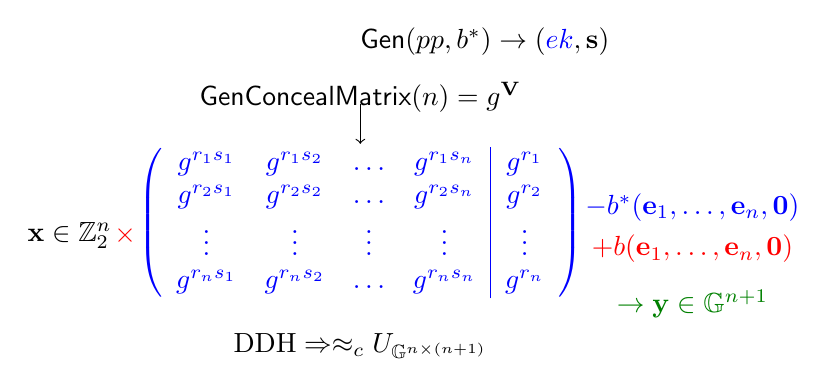
\begin{tikzpicture}
\node [textnode, name = domain] {$\mathbf{x} \in \mathbb{Z}_2^n$};

\node [textnode, name = ek, right of = domain, xshift=15em, yshift=7em] 
	{$\mathsf{Gen}(pp, b^*) \rightarrow (\blue{ek}, \mathbf{s})$}; 

\node [textnode, name = GenConceal, right of = domain, xshift = 10.5em, yshift=5em] {$\mathsf{GenConcealMatrix}(n) = g^\mathbf{V}$}; 
\node [textnode, name = matrix, below of = GenConceal, yshift=-4em, color = blue] 
{\begin{minipage}{0.50\textwidth} 
\begin{displaymath} 
\left( \begin{array}{cccc|c}
g^{r_1s_1} & g^{r_1s_2} & \ldots & g^{r_1s_n} & g^{r_1} \\
g^{r_2s_1} & g^{r_2s_2} & \ldots & g^{r_2s_n} & g^{r_2} \\
\vdots & \vdots & \vdots & \vdots & \vdots\\
g^{r_ns_1} & g^{r_ns_2} & \ldots & g^{r_ns_n} & g^{r_n} \\
\end{array} \right)
\end{displaymath}
\end{minipage}};  

\draw ($(GenConceal.south)+(0, 0.3em)$) edge[->] ($(matrix.north)+(0, -1em)$); 

\node [textnode, name = pseudorandom, below of  = GenConceal, yshift = -9em] 
{$\text{DDH} \Rightarrow \approx_c U_{\mathbb{G}^{n \times (n+1)}}$};

\node [textnode, name = minus, right of = matrix, xshift=12em, yshift=0em, color = blue] 
    {$-b^*(\mathbf{e}_1, \dots, \mathbf{e}_n, \mathbf{0})$};

\node [textnode, name = times, right of = domain, xshift=2em, color = red] {$\times$}; 
\node [textnode, name = plus, below of = minus, yshift=-1.5em, color = red] 
    {$+b(\mathbf{e}_1, \dots, \mathbf{e}_n, \mathbf{0})$};  
\node [textnode, name = image, below of = plus, yshift=-2em, color = darkgreen] {$\rightarrow \mathbf{y} \in \mathbb{G}^{n+1}$}; 

\end{tikzpicture}
\end{center}


\begin{theorem}
基于DDH假设, 上述构造是一族分支集合为$B = \mathbb{Z}_p$的$(n, \log p)$-ABO-TDF. 
\end{theorem}

\begin{proof}
容易验证, 当$b \neq b^*$时, $\mathbf{V}+(b-b^*)\mathbf{I}'$矩阵满秩, $f_{ek, b}$单射且可高效求逆; 
当$b = b^*$时, 矩阵$\mathbf{V}+(b-b^*)\mathbf{I}'$的秩为1, $\text{Img}(f_{ek, b}) \leq p$. 
有损分支隐藏性由$\mathsf{GenConcealMatrix}$输出的伪随机性(引理~\ref{equation:ConcealMatrix})保证. \qed
\end{proof}

\begin{remark}
为了确保求逆算法的高效性, 以上构造有两个重要的设定: (1) 首先在ConcealMatrix设置了辅助列$(g^{r_1}, \dots, g^{r_n})^T$, 
便于计算出$a_i = g^{x_i}$; (2) 从$a_i$中计算$x_i$需要求解离散对数, 
因此定义域$X$设定为$\mathbb{Z}_2^n$, 其中$2$可以进一步放宽至$\kappa^{O(1)}$(关于$\kappa$的多项式规模), 
以保证可以在多项式时间完成离散对数求解. 
\end{remark}

\subsubsection*{扩展与深化}
注意到在公钥加密的选择密文安全定义中敌手对解密谕言机的访问权限是全除一的, 
由此可以看出全除一有损陷门函数的应用局限于``全除一''类安全的密码方案设计.  
Hofheinz~\cite{Hofheinz-EUROCRYPT-2012}引入了全除多有损陷门函数, 
将有损分支的数量从1扩展到$\mathsf{poly}(\kappa)$, 并展示了其在选择打开选择密文安全(selective opening chosen-ciphertext security)中的应用.
在有损陷门函数的应用中, 我们通常期望有损模式下函数丢失的信息尽可能的多, 即像集尽可能的小. 这是因为单射和有损模式的反差越大, 所蕴含的结果越强, 
如更高的泄漏容忍能力、更紧的安全归约等. 但凡事有度, 物极必反, 在常规的一致归约(universal reduction)模型下, 
有损模式的像集尺寸$2^\tau$不能过小, 至少是关于计算安全参数$\kappa$的超多项式规模, 否则PPT的敌手可以通过生日攻击有效的区分单射和有损模式. 
Zhandry~\cite{Zhandry-CRYPTO-2016}创造性的提出了极度有损函数(ELF, extremely lossy functions). 
在ELF中, 有损模式下函数的像集可以缩小至关于计算安全参数$\kappa$的多项式规模, 只要在指定PPT敌手的生日攻击能力之外即可. 
ELF的有损模式之所以能够打破像集多项式界的关键在更为精细的个体归约(individual reduction)模型~\cite{Deng-EUROCRYPT-2017}下进行安全性证明.  
Zhandry基于不可区分程序混淆给出了ELF的构造, 并展示了其强大的应用.   
在无须求逆的应用场景中, 不仅不需要陷门, 甚至是单射的性质也可以弱化. 
陈等~{Chen-CT-RSA-2018}根据这一观察, 提出了规则有损函数(RLF, regular lossy functions). 
相比标准的LTDF, RLF将单射可逆模式放宽至规则有损, 即每个像的原像集合大小相同. 
正是这一弱化, 使得RLF不仅有更加高效的具体构造, 也可由哈希证明系统通用构造得出, 并在抗泄漏密码学领域有着重要的应用.     

\subsection{相关积单向陷门函数}
\begin{center}
    山重水复疑无路, 柳暗花明又一村. \\
                \hfill --- 宋 $\cdot$ 陆游《过山西村》
\end{center}


令$\mathcal{F} = \{f_{ek}: X \rightarrow Y\}$是一族单向陷门函数, 
可以自然对$\mathcal{F}$进行$t$重延拓, 得到$\mathcal{F}^t = \{g_{ek_1, \dots, ek_t}: X^t \rightarrow Y^t\}$, 
其中$f^t_{ek_1, \dots, ek_t}(x_1, \dots, x_t):= (f_{ek_1}(x_1), \dots, f_{ek_t}(x_t))$. 
我们称$\mathcal{F}^t$为$\mathcal{F}$的$t$重积($t$-wise product). 

\begin{center}
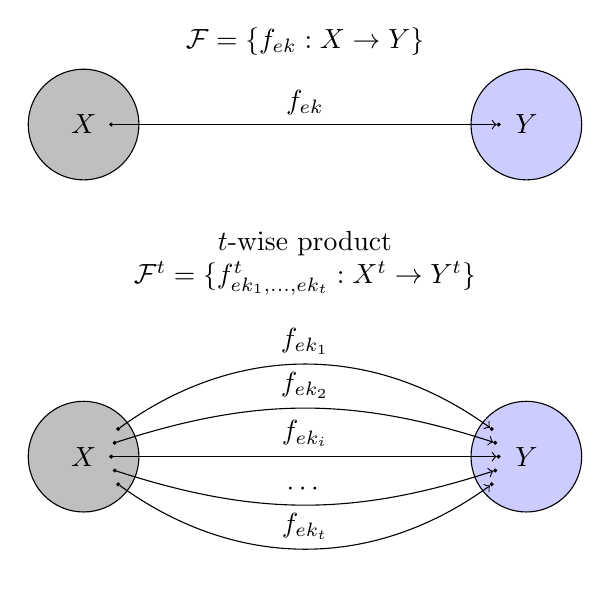
\begin{tikzpicture}
\node [textnode, name=OWF] {$\mathcal{F} = \{f_{ek}: X \rightarrow Y\}$}; 
\node [circlenode, minimum size=4em, name=domain0, below of=OWF, xshift=-8em, yshift=-3em, fill=gray!50] {$X$}; 
\node [circlenode, minimum size=4em, name=range0, below of=OWF, xshift=8em, yshift=-3em, fill=blue!20] {$Y$};
\node [dotnode, minimum size=0.1em, name=x0, right of=domain0, xshift=1em] {}; 
\node [dotnode, minimum size=0.1em, name=y0, left of=range0, xshift=-1em] {};
\draw (x0) edge[->] node[above]{$f_{ek}$} (y0);  

\node [textnode, name=product, below of=OWF, yshift=-8em] {$t$-wise product\\$\mathcal{F}^t = \{f^t_{ek_1, \dots, ek_t}: X^t \rightarrow Y^t\}$}; 

\node [circlenode, minimum size=4em, name=domain, fill=gray!50, below of = domain0, yshift=-12em] {$X$}; 
\node [circlenode, minimum size=4em, name=range, fill=blue!20, below of = range0, yshift=-12em] {$Y$};

\node [dotnode, minimum size=0.1em, name=x, right of=domain, xshift=1em] {}; 
\node [dotnode, minimum size=0.1em, name=y, left of=range, xshift=-1em] {};
\draw (x) edge[->] node[above]{$f_{ek_i}$} (y);   

\node [dotnode, minimum size=0.1em, name=x1, right of=domain, xshift=1.25em, yshift=1em] {}; 
\node [dotnode, minimum size=0.1em, name=y1, left of=range, xshift=-1.25em, yshift=1em] {};
\draw (x1) edge[->, bend left=36] node[above]{$f_{ek_1}$} (y1);   

\node [dotnode, minimum size=0.1em, name=x2, right of=domain, xshift=1.125em, yshift=0.5em] {}; 
\node [dotnode, minimum size=0.1em, name=y2, left of=range, xshift=-1.125em, yshift=0.5em] {};
\draw (x2) edge[->, bend left=18] node[above]{$f_{ek_2}$} (y2); 

\node [dotnode, minimum size=0.1em, name=x3, right of=domain, xshift=1.125em, yshift=-0.5em] {}; 
\node [dotnode, minimum size=0.1em, name=y3, left of=range, xshift=-1.125em, yshift=-0.5em] {};
\draw (x3) edge[->, bend right=18] node[above]{$\cdots$} (y3); 

\node [dotnode, minimum size=0.1em, name=x4, right of=domain, xshift=1.25em, yshift=-1em] {}; 
\node [dotnode, minimum size=0.1em, name=y4, left of=range, xshift=-1.25em, yshift=-1em] {};
\draw (x4) edge[->, bend right=36] node[above]{$f_{ek_t}$} (y4);    
\end{tikzpicture}
\end{center}

\begin{theorem}
如果$\mathcal{F} = \{f_{ek}\}$是一族单向函数, 那么它的$t$重积$\mathcal{F}^t = \{f^t_{ek_1, \dots, ek_t}\}$也是一族单向函数. 
\end{theorem}

\begin{proof}
证明的思路简述如下: 如果存在PPT的敌手$\mathcal{A}$打破$\mathcal{F}^t$的单向性, 
那么其必然以不可忽略的优势对$t$个单向函数的实例$f_{ek_i}(\cdot)$求逆, 这显然与$\mathcal{F}$的单向性冲突, 因此得证. 
\end{proof}

\begin{remark}
上述定理在$ek_1 = \cdots = ek_t$(即所有$f_{ek_i}$相同)时仍然成立, 该情形恰好对应单向函数的单向性放大(one-wayness amplification).  
\end{remark}

需要注意的是, $f^t_{ek_1, \dots, ek_t}$单向性成立的前提是各分量输入$x_i$独立随机采样, 
而当各分量输入相关时, 单向性则未必成立, 这是因为多个像的分量交叉组合可能会泄漏原像的信息. 

\begin{construction}[反例构造]\label{counterexample:CPTDF}
令$\hat{f}_{ek}: X = \{0,1\}^n \rightarrow Y$是一个单向函数, 
构造一个新的函数$f_{ek}: \{0,1\}^{2n} \rightarrow Y||\{0,1\}^n$如下: 
\begin{equation*}
    f_{ek}(x_l||x_r): = \hat{f}_{ek}(x_l)||x_r
\end{equation*}
\end{construction}
在上述构造中, $f_{ek}$以$\hat{f}_{ek}$为核, 因此如果$\hat{f}_{ek}$是单向的, 那么$f_{ek}$也是单向的. 
考察2重积$f^2_{ek_1, ek_2}$在相关输入$(x_1 = x_l||x_r, x_2 =  x_r||x_l)$下的行为: 
\begin{equation*}
    f^2_{ek_1, ek_2}(x_1, x_2) := (f_{ek_1}(x_1), f_{ek_2}(x_2)) 
        = \hat{f}_{ek_1}(x_l)||x_r||\hat{f}_{ek_2}(x_r)||x_l 
\end{equation*}
根据$f_{ek}$的设计, $f^2_{ek_1, ek_2}$的原像信息$(x_1, x_2)$可以从像中的$(x_r, x_l)$完全恢复出来, 
因此在输入呈如上相关时并不满足单向性. 上述反例构造的精髓是设计具有特殊结构的单向函数. 

反例~\ref{counterexample:CPTDF}说明单向函数的$t$重积在输入相关时并不一定仍然单向. 
Alon和Rosen~\cite{RS-TCC-2009}引入了相关积(correlated products)单向陷门函数, 定义如下: 要求函数的$t$重积在输入分量相关时仍然保持单向性

\begin{definition}[相关积单向性]
令$\mathcal{F}: X \rightarrow Y$是一族单向函数, $\mathcal{C}_t$是定义在$X^t$上的分布(分量相关). 
如果$\mathcal{F}$的$t$重积$\mathcal{F}^t: X^t \rightarrow Y^t$在$\mathcal{C}_t$相关积下仍然是单向的, 
(即对于任意PPT敌手$\mathcal{A}$, 其在如下的安全实验中优势是可忽略的) 
\begin{displaymath}
\Pr \left[
f^t_{ek_1, \dots, ek_t}(x') = y^*: 
\begin{array}{l}
    ek_i \leftarrow \mathsf{Gen}(\kappa);\\
    (x_1^*, \dots, x_t^*) \sample \mathcal{C}_t; \\
    y^* \leftarrow (f_{ek_1}(x_1^*), \dots, f_{ek_t}(x_t^*));\\
    x' \leftarrow \mathcal{A}(ek_1, \dots, ek_t, y^*);\\
\end{array} 
\right]
\end{displaymath}
则称$\mathcal{F}$是$\mathcal{C}_t$相关积安全的(correlated-product secure). 该定义可以自然延拓到陷门函数场景.   
\end{definition}

在给出CP-TDF的定义后, 接下来需要研究的问题是分析什么样的$\mathcal{F}$在何种相关积下仍然单向. 
本书中聚焦最为典型的一种$\mathcal{C}_t$相关积——均匀重复相关积$\mathcal{U}_t$, 即$x_1 \sample X$且$x_1 =  \dots = x_t$. 
Rosen和Segev~\cite{RS-TCC-2009}基于LTDF给出了CP-TDF的一个通用构造, 揭示了两者之间的联系. 

\begin{theorem}
令$\mathcal{F}$是一族$(n, \tau)$-LTDF, 那么$\mathcal{F}$在相关积$\mathcal{U}_t$下仍然单向, 
其中$t \leq (n-\omega(\log \kappa))/\tau$.  
\end{theorem}

\begin{proof}
证明通过以下的游戏序列完成, 敌手在$\text{Game}_i$中成功的事件为$S_i$.  
\begin{trivlist}
\item $\text{Game}_0$: 对应真实的相关积单向性实验, 函数以单射模式运作 
\begin{itemize}
    \item $\mathcal{CH}$独立运行$\mathcal{F}.\mathsf{GenInjective}(\kappa)$算法$t$次, 
    	生成$ek = (ek_1, \dots, ek_t)$并将其发送给$\mathcal{A}$. 
    \item $\mathcal{CH}$随机采样$x^* \sample X$, 计算$y^* \leftarrow (f_{ek_1}(x^*), \dots, f_{ek_t}(x^*))$
    	并将$y^*$发送给$\mathcal{A}$. 
    \item $\mathcal{A}$输出$x'$, 当且仅当$x' =  x^*$时成功. 
\end{itemize}
根据定义, 我们有:
\begin{equation*}
\AdvA^{\text{Game}_0}(\kappa) = \Pr[S_0]
\end{equation*}

\item $\text{Game}_1$: 与上一游戏相同, 区别在于函数切换到有损模式运作 
\begin{itemize}
    \item $\mathcal{CH}$独立运行\redul{$\mathcal{F}.\mathsf{GenLossy}(\kappa)$}算法$t$次, 
    	生成$ek = (ek_1, \dots, ek_t)$并将其发送给$\mathcal{A}$. 
\end{itemize}
\begin{equation*}
\AdvA^{\text{Game}_1}(\kappa) = \Pr[S_1]
\end{equation*}
\end{trivlist}

\begin{claim}
基于LTDF的单射/有损模式不可区分性, 任意PPT敌手$\mathcal{A}$在$\text{Game}_0$和$\text{Game}_1$中的成功概率差可忽略. 
\end{claim}

\begin{proof}
$\text{Game}_0$和$\text{Game}_1$的差别在于$(ek_1, \dots, ek_t)$的生成模式. 
基于LTDF的单射/有损模式不可区分性和hybrid argument, 可以推出$\text{Game}_0 \approx_c \text{Game}_1$, 
进而保证$|\Pr[S_0] - \Pr[S_1]| \leq \mathsf{negl}(\kappa)$.  
\end{proof}

\begin{claim}
对于任意敌手$\mathcal{A}$(即使拥有无穷计算能力), $\Pr[S_1] = \mathsf{negl}(\lambda)$. 
\end{claim}

\begin{proof}
在$\text{Game}_1$中, 函数工作在有损模式, 因此像集的大小至多为$2^{t \cdot \tau}$, 
由chainning lemma~\ref{lemma:chainning-lemma}可知$x^*$的平均最小熵$\avminentropy(x^*|y^*) \geq n - t \tau$. 
根据定理前提条件中的参数选取, 有$\avminentropy(x^*|y^*) \geq \omega(\log \kappa)$, 因此断言得证. \qed
\end{proof}

综上, 我们有$\Pr[S_0] \leq \mathsf{negl}(\kappa)$. 定理得证! \qed
\end{proof}

\begin{note}
追求简洁、消除冗余在科学和文学领域似乎都是真理. 
然而, 正如知乎上一篇文章~\cite{zhihu-essay}所说:``尽管我们偏爱简洁, 但冗余让一切皆有可能''. 相关积单向函数的定义和构造就充分诠释了冗余的力量.
\end{note}

\subsection{自适应单向陷门函数}
\begin{center}
    他强由他强, 清风拂山冈; 他横由他横, 明月照大江; 他自狠来他自恶, 我自一口真气足. \\
                \hfill --- 达摩《九阳真经》
\end{center}



构造~\ref{construction:TDF-based-KEM}仅具备IND-CPA安全性, 并不一定能够满足IND-CCA安全性. 
这是因为底层的TDF可能具备诸如同态等优良的代数性质, 使得上层PKE/KEM方案具有可延展性. 
从安全归约的角度分析, 归约算法无法对解密/解封装询问做出正确的应答. 
基于以上分析, 一个自然的问题是: TDF满足何种增强的性质才能够使得构造~\ref{construction:TDF-based-KEM}满足IND-CCA安全性. 

Kiltz, Mohassel和O'Neill~\cite{KMO-EUROCRYPT-2010}提出了自适应单向性(adaptive one-wayness), 
该性质要求TDF的单向性在敌手能够访问求逆谕言机的情况下仍然成立. 
% \begin{frame}{Adaptive One-wayness/Pseudorandomness}
% A family of TDF is adaptive one-way/pseudorandom if for all PPT $\mathcal{A}$ 
% the following advantage function is $\mathsf{negl}(\lambda)$
\begin{definition}[自适应单向性]
令$\mathcal{F}$是一族陷门函数, 定义敌手$\mathcal{A}$的优势如下:  
\begin{displaymath} 
\Pr \left[
x' \in f_{ek}^{-1}(y^*): 
\begin{array}{l}
    pp \leftarrow \mathsf{Setup}(\kappa);\\
    (ek, td) \leftarrow \mathsf{KeyGen}(pp);\\
    x^* \sample X, y^* \leftarrow f_{ek}(x^*);\\
    x' \leftarrow \mathcal{A}^{\mathcal{O}_\mathsf{inv}}(ek, y^*);
\end{array} 
\right]
\end{displaymath}
其中$\mathcal{O}_\mathsf{inv}$是求逆谕言机, $\forall x \neq x^*$, $\mathcal{O}_\mathsf{inv}(y) = \mathsf{TdInv}(td, y)$. 
如果任意PPT敌手$\mathcal{A}$在上述安全试验中的优势均为$\mathsf{negl}(\kappa)$, 
那么则称$\mathcal{F}$是自适应单向的.  
\end{definition}

为了方便在公钥加密场景中的应用, 引入自适应伪随机性如下.  
\begin{definition}[自适应伪随机性]
令$\mathcal{F}$是一族单向函数, $\mathsf{hc}$是其hardcore function. 定义敌手$\mathcal{A}$的优势如下:  
\begin{displaymath} 
\Pr \left[
\beta' = \beta: 
\begin{array}{l}
    (ek, td) \leftarrow \mathcal{F}.\mathsf{Gen}(\lambda);\\
    x^* \sample X, y^* \leftarrow f_{ek}(x^*);\\
    k_0^* \leftarrow \mathsf{hc}(x^*), k_1^* \sample K, \beta \sample \{0,1\};\\
    \beta' \leftarrow \mathcal{A}^{\mathcal{O}_\mathsf{inv}}(ek, y^*, k_\beta^*);
\end{array} 
\right] - \frac{1}{2}
\end{displaymath}
其中$\mathcal{O}_\mathsf{inv}$是求逆谕言机, $\mathsf{hc}$是$\mathcal{F}$的hardcore function. 
如果任意PPT敌手$\mathcal{A}$在上述安全试验中的成功概率均为$\mathsf{negl}(\kappa)$, 
那么则称$\mathsf{hc}$的是自适应伪随机的.  
\end{definition}

\begin{corollary}
$\mathcal{F}$的自适应单向性蕴含hardcore function的自适应伪随机性.
\end{corollary}
\begin{proof}
Goldreich-Levin定理的证明可以平行推广到求逆谕言机$\mathcal{O}_\mathsf{inv}$存在的情形下, 
$\mathsf{hc}(x^*)$自适应伪随机性由$x^*$的自适应单向性保证. \qed
\end{proof}

自适应单向陷门函数(ATDF, adaptive TDF)定义简洁, 威力强大, 将ATDF代入构造~\ref{construction:TDF-based-KEM}中, 
得到的KEM满足IND-CCA安全. 从安全归约的角度观察, ATDF的自适应单向性是为KEM的CCA安全性量身定制的, 都是``全除一''类型的安全定义. 
那么, 如何构造ATDF呢? 文献~\cite{KMO-EUROCRYPT-2010}一方面基于实例独立(instance-independent)假设给出ATDF的具体构造, 
一方面分别基于LTDF和CP-TDF给出了ATDF的两个通用构造. 

以下我们聚焦ATDF的通用构造, 首先展示如何基于LTDF构造ATDF. 
构造的技术困难点在于ATDF的安全试验中挑战者$\mathcal{CH}$向敌手$\mathcal{A}$提供了``全除一''式解密谕言机$\mathcal{O}_\mathsf{inv}$, 
而LTDF的安全试验中并没有提供类似的谕言机访问接口. 
因此, 构造的思路是通过引入精巧的结构完成解密谕言机$\mathcal{O}_\mathsf{inv}$的模拟. 
总体的思路如下: 
\begin{itemize} 
\item 令ATDF的像$y$形如$(y_0, y_1)$, 确保$y_1$由$y_0$惟一确定, 可行的设计是计算原像$x$的LTDF值作为$y_0$, 
	再以$y_0$为分支编号计算$x$的ABO-TDF值作为$y_1$. 
\begin{equation*}
    y_0 \leftarrow f(ek_\text{ltdf}, x), y_1 \leftarrow g(ek_\text{abo}, y_0, x) 
\end{equation*}

\item 上述设计利用ABO-TDF的相对分支标签的``全除一''求逆陷门嵌入了相对于像的``全除一''可逆结构. 
\end{itemize}

\begin{construction}[基于LTDF和ABO-TDF的ATDF构造]
\begin{trivlist}
\item 构造所需的组件是:
\begin{itemize}
    \item $(n, \tau_1)$-LTDF -- $\mathcal{F}: X \rightarrow Y_1$; 
    \item $(n, \tau_2)$-ABO-TDF -- $\mathcal{G}: X \rightarrow Y_2$ w.r.t. $Y_1$作为分支集合; 
\end{itemize}
其中$\log_2 |X| = n$, $\log_2 |Y_1| = m_1$, $\log_2 |Y_2| = m_2$. 

\item 构造$\text{ATDF}: X \rightarrow Y_1 \times Y_2$如下: 
\begin{itemize}
\item $\mathsf{Setup}(1^\kappa)$: 以安全参数$\kappa$为输入, 
	计算$pp_\text{ltdf} \leftarrow \mathcal{F}.\mathsf{Setup}(1^\kappa)$, 
	$pp_\text{abo} \leftarrow \mathcal{G}.\mathsf{Setup}(1^\kappa)$, 
	输出$pp = (pp_\text{ltdf}, pp_\text{abo})$.  

\item $\mathsf{Gen}(pp)$: 以公开参数$pp = (pp_\text{ltdf}, pp_\text{abo})$为输入, 
	计算$(ek_\text{ltdf}, td_\text{ltdf}) \leftarrow \mathcal{F}.\mathsf{GenInjective}(pp_\text{ltdf})$, 
	$(ek_\text{abo}, td_\text{abo}) \leftarrow \mathcal{G}.\mathsf{Gen}(pp_\text{abo}, 0^{m_1})$, 
	输出求值公钥$ek = (ek_\text{ltdf}, ek_\text{abo})$和陷门$td = (td_\text{ltdf}, td_\text{abo})$.  

\item $\mathsf{Eval}(ek, x)$: 以求值公钥$ek = (ek_\text{ltdf}, ek_\text{abo})$和$x \in \{0,1\}^n$为输入, 
	计算$y_1 \leftarrow f_{ek_\text{ltdf}}(x)$, $y_2 \leftarrow g_{ek_\text{abo}}(y_1, x)$, 输出$y = (y_1, y_2)$. 

\item $\mathsf{TdInv}(td, y)$: 以陷门$td = (td_\text{ltdf}, td_\text{abo})$和$y = (y_1, y_2)$为输入, 
	计算$x \leftarrow \mathcal{F}.\mathsf{TdInv}(td_\text{ltdf}, y_1)$, 
	验证$y_2 \stackrel{?}{=} g_{ek_\text{abo}}(y_1, x)$: 如果是输出$x$, 否则输出$\bot$. 
\end{itemize}
\end{trivlist}
\end{construction}

上述构造的正确性显然成立. 安全性由如下定理保证: 
\begin{theorem}
基于LTDF和ABO-TDF的安全性, 上述构造在$n - \tau_1 - \tau_2 \geq \omega(\log \kappa)$构成一族ATDF.
\end{theorem}

\begin{proof}
令$(x^*, y^* = (y_1^*, y_2^*))$为单向挑战实例, 其中$x^*$是原像, $y^*$是像. 
证明的思路将像$y^* = (y_1^*, y_2^*)$的计算方式从单射无损模式逐步切换到有损模式, 最终在信息论意义下论证单向性.  
\begin{trivlist}
\item $\text{Game}_0$: 真实的ATDF单向性试验. $\mathcal{CH}$与$\mathcal{A}$交互如下:
\begin{itemize}
	\item 初始化: $\mathcal{CH}$进行如下操作
    	\begin{enumerate}
    		\item 运行$pp_\text{ltdf} \leftarrow \mathcal{F}.\mathsf{Setup}(1^\kappa)$, 
				$pp_\text{abo} \leftarrow \mathcal{G}.\mathsf{Setup}(1^\kappa)$; 
			\item 计算$(ek_\text{ltdf}, td_\text{ltdf}) \leftarrow \mathcal{F}.\mathsf{GenInjective}(pp_\text{ltdf})$, 
        		$(ek_\text{abo}, td_\text{abo}) \leftarrow \mathcal{G}.\mathsf{Gen}(pp_\text{abo}, 0^{m_1})$;
    		\item 发送$pp = (pp_\text{ltdf}, pp_\text{abo})$和$ek = (ek_\text{ltdf}, ek_\text{abo})$给$\mathcal{A}$. 
    	\end{enumerate}

	\item 挑战: $\mathcal{CH}$随机选取$x^* \sample X$, 
		计算$y_1^* \leftarrow f_{ek_\text{ltdf}}(x^*)$, $y_2^* \leftarrow g_{ek_\text{abo}}(y_1^*, x^*)$, 
		发送$y^* = (y_1^*, y_2^*)$给$\mathcal{A}$. 

	\item 求逆询问: 当$\mathcal{A}$向$\mathcal{O}_\text{inv}$询问$y = (y_1, y_2)$的原像时, $\mathcal{CH}$分情况应答如下:  
	\begin{itemize}
    	\item $y_1 = y_1^*$: 直接返回$\bot$.  
    	\item $y_1 \neq y_1^*$: 首先计算$x \leftarrow \mathcal{F}.\mathsf{TdInv}(td_\text{ltdf}, y_1)$, 
        	如果$y_2 =  g_{ek_\text{abo}}(y_1, x)$则返回$x$, 否则返回$\bot$. 
	\end{itemize}
	根据ATDF像的生成方式可知, 第一部分完全确定了第二部分, 当$y_1 = y_1^*$时, 
	如$y_2 = y_2^*$则$\mathcal{A}$的询问为禁讯点, 如$y_2 \neq y_2^*$则像的格式不正确. 
	基于以上分析, $\mathcal{CH}$在应答形如$(y_1^*, y_2)$的求逆询问时, 无须进一步检查第二部分$y_2$, 直接返回$\bot$即可保证应答的正确性. 
\end{itemize}

\item $\text{Game}_1$: 在$\text{Game}_0$中$\mathcal{CH}$使用$\mathcal{F}$的陷门进行求逆, 
	因此$\mathcal{F}$必须工作在单射可逆模式. 为了将$y_1^*$的计算模式切换到有损模式, 
	需要利用$\mathcal{G}$的陷门进行求逆. 注意到在$\text{Game}_0$中$\mathcal{G}$的``全除一''陷门根据预先设定的有损分支$0^{m_1}$生成, 
	因此必须先激活再使用, 因此$\text{Game}_1$的设计目的是为激活做准备:  
\begin{itemize}
    \item $\mathcal{CH}$在初始化阶段即\redul{随机采样$x^* \sample X$, 并计算$y_1^* \leftarrow f_{ek_\text{ltdf}}(x^*)$}.
\end{itemize}
与$\text{Game}_0$相比, $\text{Game}_1$仅将上述操作从挑战阶段提前至初始化阶段, 敌手的视图没有发生任何变化, 因此有: 
\begin{equation*} 
    \text{Game}_0 \equiv \text{Game}_1
\end{equation*}

\item $\text{Game}_2$: 上一游戏已经做好激活$\mathcal{G}$陷门的准备, 
	因此在$\text{Game}_2$中将预设的有损分支值由$0^{m_1}$替换为$y_1^*$完成激活:
\begin{itemize} 
    \item $(ek_\text{abo}, td_\text{abo}) \leftarrow G.\mathsf{Gen}(pp_\text{abo}, \red{y_1^*})$
\end{itemize}
由ABO-TDF的有损分支隐藏性质, 可以得到:
\begin{equation*}
   	\text{Game}_1 \approx_c \text{Game}_2
\end{equation*}

\item $\text{Game}_3$: 使用$\mathcal{G}$的陷门$td_\text{abo}$应答求逆询问, 
	当$\mathcal{A}$发起询问$y = (y_1, y_2)$时, $\mathcal{CH}$分情形应答如下:  
\begin{itemize}
    \item $y_1 = y_1^*$: 直接返回$\bot$. 
    \item $y_1 \neq y_1^*$: 计算$x \leftarrow \mathcal{G}.\mathsf{TdInv}(td_\text{abo}, y_1, y_2)$, 
        如果$y_1 = f_{ek_\text{ltdf}}(x)$则返回$x$, 否则返回$\bot$.
\end{itemize} 
像的生成方式和$\mathcal{G}$求逆算法的正确性和保证了$\mathcal{O}_\mathsf{inv}$应答的正确性, 因此有: 
\begin{equation*}
    \text{Game}_2 \equiv \text{Game}_3 
\end{equation*}

\item $\text{Game}_4$: 将$y_1^*$的生成方式切换到有损模式
\begin{itemize}
	\item $\mathcal{CH}$在初始化阶段计算\redul{$(ek_\text{ltdf}, \bot) \leftarrow \mathcal{F}.\mathsf{GenLossy}(pp_\text{ltdf})$}
\end{itemize}
LTDF的单射/有损模式的计算不可区分性保证了
\begin{equation*}  
    \text{Game}_3 \approx_c \text{Game}_4
\end{equation*}
\end{trivlist}

\begin{claim}
    对任意的敌手$\mathcal{A}$(即使拥有无穷的计算能力)均有$\AdvA(\text{Game}_4) = \mathsf{negl}(\kappa)$. 
\end{claim}

\begin{proof}
在$\text{Game}_4$中, 函数$f_{ek_\text{ltdf}}(\cdot)$有损且像集大小至多为$2^{\tau_1}$, 
函数$g_{ek_\text{abo}}(y_1^*, \cdot)$有损且像集大小至多为$2^{\tau_2}$. 
因此$y_1^*$和$y_2^*$均在信息论意义下损失了原像$x^*$的信息, 
在敌手$\mathcal{A}$的视图中, $x^*$的平均最小熵为
$\avminentropy(x^*|(y_1^*, y_2^*)) \geq \minentropy(x^*) - \tau_1 - \tau_2 = n - \tau_1 - \tau_2 \geq \omega(\log \kappa)$. 
从而对于任意敌手$\mathcal{A}$均有: 
\begin{equation*}
    \AdvA(\text{Game}_4) = \mathsf{negl}(\kappa)
\end{equation*}
断言得证! \qed
\end{proof}
综上, 定理得证! \qed
\end{proof}

\begin{remark}
上述构造的设计思想值得读者反复拆解, 体会其精妙之处. 
上述ATDF构造在形式上与Naor-Yung的双钥加密有异曲同工之处: 
分别使用$f_{ek_\text{ltdf}}(\cdot)$和$g_{ek_\text{abo}}(\cdot, \cdot)$两个函数计算原像的函数值作为像.  
一个自然的想法是上述构造显得冗余, 是否仅用ABO-TDF即可呢? 答案是否定的, 如果仅依赖ABO-TDF构造ATDF, 需要满足以下四点: 
\begin{itemize} 
	\item 求值分支可由输入公开确定计算得出, 以确保ATDF是公开可计算函数.
	\item 像所对应的求值分支可由像中计算得出, 以确保ATDF的求逆算法可以基于ABO-TDF的求逆算法设计. 
	\item 在安全归约中势必需要将ATDF的单向性建立在ABO-TDF的信息有损性上, 也即$y^*$是$x^*$在有损分支的求值.
\end{itemize}
上述三点潜在要求ATDF的像包含两个部分, 一部分是原像对应的分支值, 一部分是ABO-TDF在该分支值下的像, 这使得在安全证明时存在如下两个障碍:
\begin{enumerate}
	\item 分支值泄漏原像的多少信息难以确定 
	\item 敌手可以从挑战的像中计算出有损分支值, 从而可以发起关于有损分支的求逆询问, 而归约算法无法应答
\end{enumerate} 

通过上述的拆解分析, 便可看出ATDF设计的必然性. 引入LTDF并将分支值设定为原像的LTDF值有三重作用:
\begin{itemize} 
	\item LTDF的陷门确保了ATDF构造存在功能完备的陷门.
	\item 可将分支值泄漏的关于原像信息量控制在指定范围.  
	\item 分支值完全确定了像, 从而使得ABO-TDF的陷门在归约证明中可用于模拟求逆谕言机$\mathcal{O}_\mathsf{inv}$.  
\end{itemize} 
LTDF+ABO-TDF $\Rightarrow$ ATDF的设计思路有如二级运载火箭, 第一级运载火箭(LTDF)在完成推动后从单射切换到有损模式, 
同时激活第二级运载火箭(ABO-TDF).  
\end{remark}

我们再展示如何基于CP-TDF构造ATDF. 构造的难点是在归约证明中归约算法如何在不掌握全部CP-TDF实例陷门的情况下正确模拟$\mathcal{O}_\mathsf{inv}$. 
大体的设计思路和以上基于有损陷门函数构造LTDF相似, 通过多重求值引入冗余结构, 从而使得归约算法在掌握部分CP-TDF实例陷门时能够正确应答求逆询问. 
\begin{itemize} 
    \item 设计像$y$形如$(y_0, y_1, \dots, y_n)$, 确保$y_0$能够惟一确定$(y_1, \dots, y_n)$
    \begin{itemize}
    	\item 令$y_0$是原像的CP-TDF函数值, 目的是确保$y_0$不会破坏最终ATDF函数的单向性
    	\item 令$(y_1, \dots, y_n)$是关于原像$x$的$|y_0| = n$重冗余函数求值 
    \end{itemize}
    \item 嵌入``全除一''求逆结构
    \begin{itemize}
        \item 对$y_0^*$进行比特分解: 归约算法使用Dolev-Dwork-Naor(DDN)类技术逐比特嵌入对应的陷门, 
        	使得对于点$y = (y_0, y_1, \dots, y_n)$处的求逆询问: 
        \begin{enumerate}
		    \item $y_0 = y_0^*$: 归约算法可根据$\mathcal{O}_\mathsf{inv}$的定义直接拒绝, 返回$\bot$ 
    		\item $y_0 \neq y_0^*$: $\mathcal{R}$可至少寻找到一个可用陷门用于应答$\mathcal{O}_\mathsf{inv}$. 
		\end{enumerate} 
    \end{itemize}
\end{itemize} 

\begin{construction}{基于CP-TDF的ATDF}
\begin{trivlist}
\item 构造所需组件: 单射CP-TDF $\mathcal{F}: X \rightarrow \{0,1\}^n$

\item 构造ATDF: $X \rightarrow \{0,1\}^{n(n+1)}$如下: 
\begin{itemize}
\item $\mathsf{Setup}(1^\kappa)$: 运行$pp \leftarrow \mathcal{F}.\mathsf{Setup}(1^\kappa)$, 输出$pp$作为公开参数. 

\item $\mathsf{KeyGen}(pp)$: 以公开参数$pp$为输入 
\begin{enumerate}
	\item 计算$(\hat{ek}, \hat{td}) \leftarrow \mathcal{F}.\mathsf{KeyGen}(\lambda)$;

	\item 对于$b \in \{0,1\}$和$i \in [n]$, 
		计算$(ek_{i,b}, td_{i,b}) \leftarrow \mathcal{F}.\mathsf{KeyGen}(\lambda)$;  
        
	\item 输出$(\hat{ek}, (ek_{i,0}, ek_{i,1}), \dots, (ek_{n,0}, ek_{n,1}))$作为求值公钥, 
		输出$(\hat{td}, (td_{i,0}, td_{i,1}), \dots, (td_{n,0}, td_{n,1}))$作为求逆陷门.
\end{enumerate}

\item $\mathsf{Eval}(ek, x)$: 以求值公钥$ek = \hat{ek}||(ek_{1,0}, ek_{1,1}) \dots (ek_{n,0}, ek_{n,1})$和原像$x$为输入, 计算
    \begin{enumerate}
    	\item 计算$y_0 \leftarrow f_{\hat{ek}}(x)$; 
    	\item 令$b_i \leftarrow y_0[i]$, 对$i \in [n]$计算$y_i \leftarrow f_{ek_{i,b_i}}(x)$; 
    	\item 输出$y = y_0||y_1||\dots||y_n$. 
	\end{enumerate}

\item $\mathsf{TdInv}(td, y)$: 以陷门$td = (\hat{td}, \{(td_{i,0}, td_{i,1})\}_{i \in [n]})$和像$y = y_0||y_1||\dots||y_n$为输入: 
	\begin{enumerate}
		\item 计算$x_0 \leftarrow \mathcal{F}.\mathsf{TdInv}(\hat{td}, y_0)$; 
		\item 令$b_i \leftarrow y_0[i]$, 
			对所有$i \in [n]$计算$x_i \leftarrow \mathcal{F}.\mathsf{TdInv}(td_{i,b_i}, y_i)$; 
        \item 检查$x_i = x_0$是否对于$i \in [n]$均成立, 若是则输出$x_0$, 否则输出$\bot$.
	\end{enumerate}
\end{itemize}
\end{trivlist}
\end{construction}


\begin{figure}[!htbp]
\centering
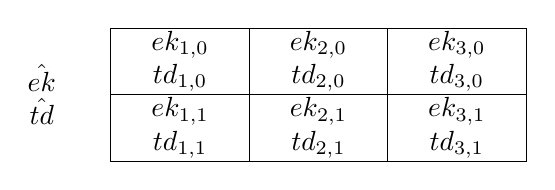
\begin{tikzpicture}
    \node [name=ekhat, textnode] {$\hat{ek}$\\$\hat{td}$}; 

    \node [name=ek10, rectanglenode, minimum width=5em, minimum height=2.4em, draw, 
        right of = ekhat, xshift=5em, yshift=1.2em] {$ek_{1,0}$\\$td_{1,0}$}; 
    \node [name=ek11, rectanglenode, minimum width=5em, minimum height=2.4em, draw, 
        right of = ekhat, xshift=5em, yshift=-1.2em] {$ek_{1,1}$\\$td_{1,1}$}; 

    \node [name=ek20, rectanglenode, minimum width=5em, minimum height=2.4em, draw, 
        right of = ekhat, xshift=10em, yshift=1.2em] {$ek_{2,0}$\\$td_{2,0}$}; 
    \node [name=ek21, rectanglenode, minimum width=5em, minimum height=2.4em, draw, 
        right of = ekhat, xshift=10em, yshift=-1.2em] {$ek_{2,1}$\\$td_{2,1}$}; 

    \node [name=ek30, rectanglenode, minimum width=5em, minimum height=2.4em, draw, 
        right of = ekhat, xshift=15em, yshift=1.2em] {$ek_{3,0}$\\$td_{3,0}$}; 
    \node [name=ek31, rectanglenode, minimum width=5em, minimum height=2.4em, draw, 
        right of = ekhat, xshift=15em, yshift=-1.2em] {$ek_{3,1}$\\$td_{3,1}$}; 
\end{tikzpicture}
\caption{$n = 3$时的求值公钥和求逆陷门图示}
\end{figure}

\begin{figure}[!htbp]
\begin{minipage}[t]{0.5\linewidth}
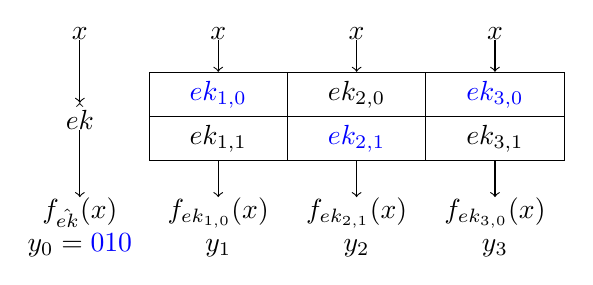
\begin{tikzpicture}
    \node [name=ekhat, textnode] {$\hat{ek}$}; 

    \node [name=ek10, rectanglenode, minimum width=5em, minimum height=1.6em, draw, 
        right of = ekhat, xshift=5em, yshift=0.8em] {\blue{$ek_{1,0}$}}; 
    \node [name=ek11, rectanglenode, minimum width=5em, minimum height=1.6em, draw, 
        right of = ekhat, xshift=5em, yshift=-0.8em] {$ek_{1,1}$}; 

    \node [name=ek20, rectanglenode, minimum width=5em, minimum height=1.6em, draw, 
        right of = ekhat, xshift=10em, yshift=0.8em] {$ek_{2,0}$}; 
    \node [name=ek21, rectanglenode, minimum width=5em, minimum height=1.6em, draw, 
        right of = ekhat, xshift=10em, yshift=-0.8em] {\blue{$ek_{2,1}$}}; 

    \node [name=ek30, rectanglenode, minimum width=5em, minimum height=1.6em, draw, 
        right of = ekhat, xshift=15em, yshift=0.8em] {\blue{$ek_{3,0}$}}; 
    \node [name=ek31, rectanglenode, minimum width=5em, minimum height=1.6em, draw, 
        right of = ekhat, xshift=15em, yshift=-0.8em] {$ek_{3,1}$}; 

    \node [textnode, name=xhat, above of = ekhat, yshift=3em] {$x$};
    \node [textnode, name=yhat, below of = ekhat, yshift=-4em] {$f_{\hat{ek}}(x)$\\$y_0 = \blue{010}$}; 
    \draw (xhat) edge[->] (ekhat); 
    \draw (ekhat) edge[->] (yhat); 

    \node [textnode, name=x1, above of = ek10, yshift=2.2em] {$x$};
    \node [textnode, name=y1, below of = ek11, yshift=-3.2em] {$f_{ek_{1,0}}(x)$\\$y_1$}; 
    \draw (x1) edge[->] (ek10); 
    \draw (ek11) edge[->] (y1); 


    \node [textnode, name=x2, above of = ek20, yshift=2.2em] {$x$};
    \node [textnode, name=y2, below of = ek21, yshift=-3.2em] {$f_{ek_{2,1}}(x)$\\$y_2$}; 
    \draw (x2) edge[->] (ek20); 
    \draw (ek21) edge[->] (y2); 

    \node [textnode, name=x3, above of = ek30, yshift=2.2em] {$x$};
    \node [textnode, name=y3, below of = ek31, yshift=-3.2em] {$f_{ek_{3,0}}(x)$\\$y_3$}; 
    \draw (x3) edge[->] (ek30); 
    \draw (ek31) edge[->] (y3);    
\end{tikzpicture}
\caption{$n=3$, $y=010$时的求值图示}
\end{minipage}
\begin{minipage}[t]{0.5\linewidth}
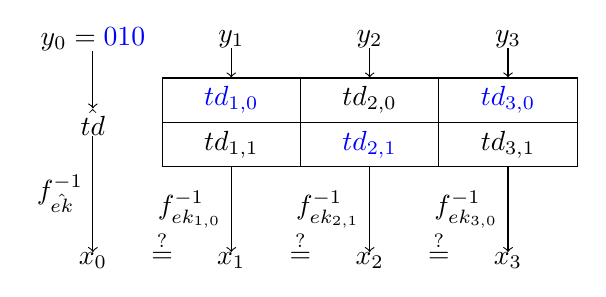
\begin{tikzpicture}
    \node [name=tdhat, textnode] {$\hat{td}$}; 

    \node [name=td10, rectanglenode, minimum width=5em, minimum height=1.6em, draw, 
        right of = tdhat, xshift=5em, yshift=0.8em] {\blue{$td_{1,0}$}}; 
    \node [name=td11, rectanglenode, minimum width=5em, minimum height=1.6em, draw, 
        right of = tdhat, xshift=5em, yshift=-0.8em] {$td_{1,1}$}; 

    \node [name=td20, rectanglenode, minimum width=5em, minimum height=1.6em, draw, 
        right of = tdhat, xshift=10em, yshift=0.8em] {$td_{2,0}$}; 
    \node [name=td21, rectanglenode, minimum width=5em, minimum height=1.6em, draw, 
        right of = tdhat, xshift=10em, yshift=-0.8em] {\blue{$td_{2,1}$}}; 

    \node [name=td30, rectanglenode, minimum width=5em, minimum height=1.6em, draw, 
        right of = tdhat, xshift=15em, yshift=0.8em] {\blue{$td_{3,0}$}}; 
    \node [name=td31, rectanglenode, minimum width=5em, minimum height=1.6em, draw, 
        right of = tdhat, xshift=15em, yshift=-0.8em] {$td_{3,1}$}; 

    \node [textnode, name=y0, above of = tdhat, yshift=3em] {$y_0 = \blue{010}$};
    \node [textnode, name=y1, above of = td10, yshift=2.2em] {$y_1$};
    \node [textnode, name=y2, above of = td20, yshift=2.2em] {$y_2$};
    \node [textnode, name=y3, above of = td30, yshift=2.2em] {$y_3$};

    \node [textnode, name=x0, below of = tdhat, yshift=-5em] {$x_0$}; 
    \draw (y0) edge[->] (tdhat); 
    \draw (tdhat) edge[->] node[left]{$f_{\hat{ek}}^{-1}$} (x0); 

    \node [textnode, name=x1, below of = td11, yshift=-4.2em] {$x_1$}; 
    \draw (y1) edge[->] (td10); 
    \draw (td11) edge[->] node[left]{$f_{ek_{1,0}}^{-1}$} (x1); 
    \node [textnode, left of = x1, xshift=-2.5em, yshift=0.5em] {$\stackrel{?}{=}$}; 

    \node [textnode, name=x2, below of = td21, yshift=-4.2em] {$x_2$}; 
    \draw (y2) edge[->] (td20); 
    \draw (td21) edge[->] node[left]{$f_{ek_{2,1}}^{-1}$} (x2); 
    \node [textnode, left of = x2, xshift=-2.5em, yshift=0.5em] {$\stackrel{?}{=}$}; 

    \node [textnode, name=x3, below of = td31, yshift=-4.2em] {$x_3$}; 
    \draw (y3) edge[->] (td30); 
    \draw (td31) edge[->] node[left]{$f_{ek_{3,0}}^{-1}$} (x3); 
    \node [textnode, left of = x3, xshift=-2.5em, yshift=0.5em] {$\stackrel{?}{=}$};    
\end{tikzpicture}
\caption{$n=3$, $y = 010$时的求逆图示}
\end{minipage}
\end{figure}

上述ATDF构造的正确性显然. 构造中, 函数的像$y = y_0||y_1||\dots||y_n$是对原像的$n+1$重求值, 
其中$y_0$确定了使用哪些求值公钥$ek_{i,b}$计算$y_i$, 因此当底层的CP-TDF是单射函数时, $y_0$可惟一确定$y_1, \dots, y_n$.  
下面的定理就是利用上述结构特性模拟求逆谕言机$\mathcal{O}_\mathsf{inv}$.

\begin{theorem}
如果$\mathcal{F}$是一族相对于$\mathcal{U}_t$安全的CP-TDF, 那么上述构造一族A自适应单向陷门函数. 
\end{theorem}
\begin{proof}
使用反证法通过单一游戏完成归约证明. 
假设存在PPT的敌手$\mathcal{A}$能以不可忽略的优势打破ATDF的自适应单向性, 
那么可以黑盒调用$\mathcal{A}$的能力构造PPT的$\mathcal{B}$打破CP-TDF相对于$\mathcal{U}_{n+1}$的单向性. 
$\mathcal{B}$的CP-TDF挑战是公开参数$pp$、求值公钥$(ek_0, ek_1, \dots, ek_n)$和像$y^* = (y_0^*, y_1^*, \dots, y_n^*)$, 
其中$y_i^* \leftarrow f_{ek_i}(x^*)$, $x^* \sample X$. 
$\mathcal{B}$并不知晓$x^*$, 其攻击目标是求解$x^*$. 

\begin{figure}[!hbtp]
\centering
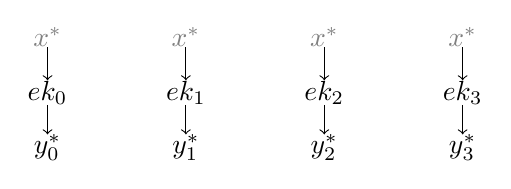
\begin{tikzpicture}
\node [textnode, name=ek0] {$ek_0$}; 
\node [textnode, name=x0, above of = ek0, yshift=2em, color=gray] {$x^*$}; 
\node [textnode, name=y0, below of = ek0, yshift=-2em] {$y_0^*$};
\draw (x0) edge[->] (ek0); 
\draw (ek0) edge[->] (y0); 

\node [textnode, name=ek1, right of = ek0, xshift=5em] {$ek_1$}; 
\node [textnode, name=x1, above of = ek1, yshift=2em, color=gray] {$x^*$}; 
\node [textnode, name=y1, below of = ek1, yshift=-2em] {$y_1^*$};
\draw (x1) edge[->] (ek1); 
\draw (ek1) edge[->] (y1); 

\node [textnode, name=ek2, right of = ek1, xshift=5em] {$ek_2$}; 
\node [textnode, name=x2, above of = ek2, yshift=2em, color=gray] {$x^*$}; 
\node [textnode, name=y2, below of = ek2, yshift=-2em] {$y_2^*$};
\draw (x2) edge[->] (ek2); 
\draw (ek2) edge[->] (y2); 

\node [textnode, name=ek3, right of = ek2, xshift=5em] {$ek_3$}; 
\node [textnode, name=x3, above of = ek3, yshift=2em, color=gray] {$x^*$}; 
\node [textnode, name=y3, below of = ek3, yshift=-2em] {$y_3^*$};
\draw (x3) edge[->] (ek3); 
\draw (ek3) edge[->] (y3); 

% \node [textnode, left of = y0, xshift=-2em, color=red] {$010$}; 
\end{tikzpicture}
\caption{$n=3$时$\mathcal{B}$的CP-TDF挑战实例}
\end{figure}

令$b_i^*$是$y_0^*$的第$i$比特, $\mathcal{B}$(扮演挑战者)与$\mathcal{A}$在ATDF的自适应单向性游戏中交互如下: 
\begin{itemize}
\item 初始化: $\mathcal{B}$将CP-TDF的$pp$设为ATDF的公开参数, 
	设定$\red{\hat{ek}} := ek_0$, 
	对$i \in [n]$设定$\red{ek_{i,b_i^*}} := ek_i$, 
	计算$\blue{(ek_{i, 1-b_i^*}, td_{i,1-b_i^*})} \leftarrow \mathcal{F}.\mathsf{KeyGen}(\kappa)$.

\item 挑战阶段: $\mathcal{B}$发送$(y_0^*, y_1^*, \dots, y_n^*)$给$\mathcal{A}$作为挑战. 

\item 求逆询问: $\mathcal{A}$向$\mathcal{B}$发起求逆询问$y = (y_0, y_1, \dots, y_n)$, 
	$\mathcal{B}$分情况应答如下:  

\begin{enumerate}
    \item $y_0 = y_0^*$: 直接返回$\bot$, 应答的正确性由以下两种细分情况保证: 
	\begin{itemize}
    	\item 对于所有的$i \in [n]$均有$y_i = y_i^*$: 询问为禁询点, 因此根据$\mathcal{O}_\mathsf{inv}$的定义需返回$\bot$.
		\item 对于某个$i \in [n]$使得$y_i \neq y_i^*$: $\mathcal{F}$的单射性质和像的生成方式保证了
			像的首项$y_0$确定了其余$n$项$y_1, \dots, y_n$.  
	\end{itemize}

    \item $y_0 \neq y_0^*$: 必然存在$\exists j \in [n]$ s.t. $b_j \neq b_j^*$且$y_j = f_{{ek_j, b_j}}(x)$, 
    	其中$x$是未知原像. 此时, $\mathcal{B}$拥有关于$ek_{j,b_j}$的求逆陷门$td_{j,b_j}$, 
    	$\mathcal{B}$可计算$x \leftarrow f_{ek_j, b_j}^{-1}(y_j)$
	\begin{itemize}
    	\item 如果$y_0 = f_{ek_0}$且$y_i = f_{ek_{i,b_i}}(x)$对其余所有$i \neq j$也均成立, 
    		那么返回$x$, 否则返回$\bot$. 
	\end{itemize}
\end{enumerate}
\item 求解: $\mathcal{A}$输出$x$作为ATDF的挑战应答, $\mathcal{B}$将$x$转发给CP-TDF的挑战者. 
\end{itemize}
容易验证, $\mathcal{B}$的优势与$\mathcal{A}$的优势相同. 定理得证! \qed
\end{proof}

\begin{figure}
\begin{minipage}[t]{0.5\linewidth}
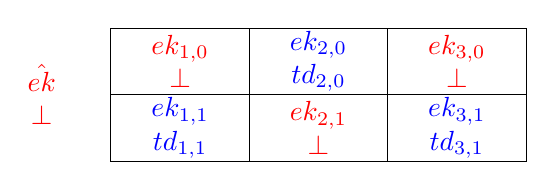
\begin{tikzpicture}
    \node [name=ekhat, textnode] {\red{$\hat{ek}$}\\\red{$\bot$}}; 

    \node [name=ek10, rectanglenode, minimum width=5em, minimum height=2.4em, draw, 
        right of = ekhat, xshift=5em, yshift=1.2em] {\red{$ek_{1,0}$}\\\red{$\bot$}}; 
    \node [name=ek21, rectanglenode, minimum width=5em, minimum height=2.4em, draw, 
        right of = ekhat, xshift=10em, yshift=-1.2em] {\red{$ek_{2,1}$}\\\red{$\bot$}}; 
    \node [name=ek30, rectanglenode, minimum width=5em, minimum height=2.4em, draw, 
        right of = ekhat, xshift=15em, yshift=1.2em] {\red{$ek_{3,0}$}\\\red{$\bot$}}; 

    \node [name=ek11, rectanglenode, minimum width=5em, minimum height=2.4em, draw, 
        right of = ekhat, xshift=5em, yshift=-1.2em] {\blue{$ek_{1,1}$}\\\blue{$td_{1,1}$}}; 
    \node [name=ek20, rectanglenode, minimum width=5em, minimum height=2.4em, draw, 
        right of = ekhat, xshift=10em, yshift=1.2em] {\blue{$ek_{2,0}$}\\\blue{$td_{2,0}$}}; 
    \node [name=ek31, rectanglenode, minimum width=5em, minimum height=2.4em, draw, 
        right of = ekhat, xshift=15em, yshift=-1.2em] {\blue{$ek_{3,1}$}\\\blue{$td_{3,1}$}}; 
\end{tikzpicture}
\caption{$y_0^* = 010$时生成求值公钥和求逆陷门的过程图示}
\end{minipage}
\begin{minipage}[t]{0.5\linewidth}
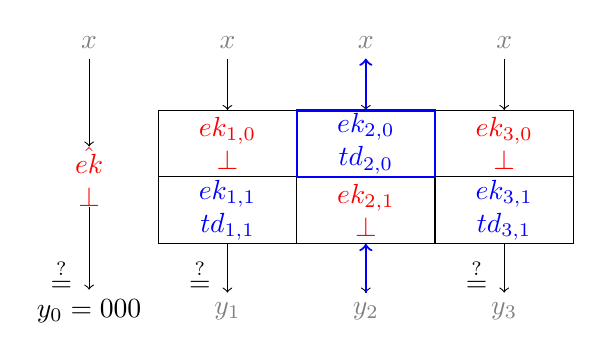
\begin{tikzpicture}
    \node [name=ekhat, textnode] {\red{$\hat{ek}$}\\\red{$\bot$}}; 

    \node [name=ek10, rectanglenode, minimum width=5em, minimum height=2.4em, draw, 
        right of = ekhat, xshift=5em, yshift=1.2em] {\red{$ek_{1,0}$}\\\red{$\bot$}};
    \node [name=ek11, rectanglenode, minimum width=5em, minimum height=2.4em, draw, 
        right of = ekhat, xshift=5em, yshift=-1.2em] {\blue{$ek_{1,1}$}\\\blue{$td_{1,1}$}}; 

    \node [name=ek20, rectanglenode, minimum width=5em, minimum height=2.4em, draw, 
        right of = ekhat, xshift=10em, yshift=1.2em] {\blue{$ek_{2,0}$}\\\blue{$td_{2,0}$}};  
    \node [name=ek21, rectanglenode, minimum width=5em, minimum height=2.4em, draw, 
        right of = ekhat, xshift=10em, yshift=-1.2em] {\red{$ek_{2,1}$}\\\red{$\bot$}}; 

    \node [name=ek30, rectanglenode, minimum width=5em, minimum height=2.4em, draw, 
        right of = ekhat, xshift=15em, yshift=1.2em] {\red{$ek_{3,0}$}\\\red{$\bot$}}; 
    \node [name=ek31, rectanglenode, minimum width=5em, minimum height=2.4em, draw, 
        right of = ekhat, xshift=15em, yshift=-1.2em] {\blue{$ek_{3,1}$}\\\blue{$td_{3,1}$}}; 

    \node [name=x0, above of = ekhat, yshift=2em] {\gray{$x$}};
    \node [name=y0, below of = ekhat, yshift=-2em] {$y_0 = 000$};
    \draw (x0) edge[->] (ekhat);
    \draw (ekhat) edge[->] (y0); 

    \node [name=x1, above of = ek10, yshift=0.8em] {\gray{$x$}};
    \node [name=y1, below of = ek11, yshift=-0.8em] {\gray{$y_1$}};
    \draw (x1) edge[->] (ek10);
    \draw (ek11) edge[->] (y1); 

    \node [name=x2, above of = ek20, yshift=0.8em] {\gray{$x$}};
    \node [name=y2, below of = ek21, yshift=-0.8em] {\gray{$y_2$}};
    \draw (x2) edge[->] (ek20);
    \draw (ek21) edge[->] (y2); 

    \node [name=x3, above of = ek30, yshift=0.8em] {\gray{$x$}};
    \node [name=y3, below of = ek31, yshift=-0.8em] {\gray{$y_3$}};
    \draw (x3) edge[->] (ek30);
    \draw (ek31) edge[->] (y3); 

    \node [rectanglenode, minimum width=5em, minimum height=2.4em, draw, 
        right of = ekhat, xshift=10em, yshift=1.2em, color=blue, thick] {}; 
    \draw (y2) edge[->, thick, color=blue] (ek21);
    \draw (ek20) edge[->, thick, color=blue] (x2); 

    \node [textnode, left of = y0, xshift=-1em, yshift=1.3em] {$\stackrel{?}{=}$}; 
    \node [textnode, left of = y1, xshift=-1em, yshift=1.3em] {$\stackrel{?}{=}$}; 
    \node [textnode, left of = y3, xshift=-1em, yshift=1.3em] {$\stackrel{?}{=}$}; 
\end{tikzpicture}
\caption{$y_0 = 000$时的求逆过程图示}
\end{minipage}
\end{figure}

\begin{remark}{优化}
以上ATDF构造的像$(y_0, y_1, \dots, y_n)$包含了对原像的$(n+1)$重CP-TDF求值:  
\begin{itemize}
    \item $y_0$构造中起到的作用求值的公钥选择向量, 在归约证明中起到的作用是``全除一''求逆陷门的激活扳机(trigger), 当$y_0 \neq y_0^*$时即可激活求逆陷门. 
\end{itemize}

$y_0$的编码长度决定了像的冗余重数. 能否缩减$|y_0|$以提高效率呢? 
答案是肯定的, 可以使用密码组件进行值域扩张(domain extension)的通用技术, 使用$y_0$的抗碰撞哈希值代替$y_0$. 
在上述构造中, 我们贴合ATDF的安全定义进行更为精细的处理, 使用TCRHF(target collision resistant hash function)代替CRHF. 
具体的, 令$\mathsf{TCR}: \{0,1\}^n \rightarrow \{0,1\}^m$, 
使用$\mathsf{TCR}(y_0)$代替$y_0$作为作为公钥选择向量和陷门激活扳机. 
从而利用$\mathsf{TCR}$压缩的性质将像的重数从$1+n$缩减到$1+m$.
安全论证仍然成立, 这是因为$\mathsf{TCR}$的抗碰撞性质保证了在计算意义下: 
\begin{equation*}
    y_0 \neq y_0^* \Longleftrightarrow \mathsf{TCR}(y_0) \neq \mathsf{TCR}(y_0^*)  
\end{equation*}   

类似的优化技术同样可以用于LTDF+ABO-TDF $\Rightarrow$ ATDF的构造中: 可以使用$y_0$的TCR哈希值代替$y_0$作为分支值. 
这样处理的好处是增加分支集合选择的灵活性.      
\end{remark}

\begin{note}
LTDF+ABO-TDF $\Rightarrow$ ATDF与CP-TDF $\Rightarrow$ ATDF的构造分别与Naor-Yung范式~\cite{NY-STOC-1990}和
Dolev-Dwork-Naor范式~\cite{DDN-STOC-1991}在思想上极为相似, 总体思路都是通过冗余的结构来保证求逆谕言机的完美模拟.  
\end{note}


\subsection*{自适应单向陷门关系}
将ATDF中的确定性函数泛化为可公开高效验证的二元关系可得到自适应单向陷门关系(ATDR, adaptive trapdoor relation).  
\begin{itemize}
    \item 确定性函数 $\leadsto$ 概率关系
    \item 可高效计算 $\leadsto$ 可高效采样 
\end{itemize}


\begin{definition}[单向陷门关系]
一族单向陷门关系包含以下算法:  
\begin{itemize}
	\item $\mathsf{Setup}(\kappa)$: 以安全参数$\kappa$为输入, 输出公开参数$pp = (X, Y, EK, TD, \mathsf{R})$, 
		其中$\mathsf{R} = \{\mathsf{R}_{ek}: X \times Y\}_{ek \in EK}$是定义在$X \times Y$上由$ek$索引的一族二元单向关系.  
    
    \item $\mathsf{KeyGen}(pp)$: 以公开参数$pp$为输入, 输出公钥$ek$和陷门$td$. 

    \item $\mathsf{Sample}(ek)$: 输出二元关系的一个随机采样$(x, y) \sample \mathsf{R}_{ek}$. 

    % \item $\mathsf{Verify}(ek, x, y)$: 以$ek$和$(x, y)$为输入, 输出``1''当且仅当$(x, y) \in \mathsf{R}_{ek}$. 

    \item $\mathsf{TdInv}(td, y)$: 以$td$和$y \in Y$为输入, 输出$x \in X \cup \bot$. 
\end{itemize}
\end{definition}

\begin{trivlist}
\item \textbf{正确性:} $\forall (ek, td) \leftarrow \mathsf{KeyGen}(pp)$, $\forall (x, y) \leftarrow \mathsf{Sample}(ek)$, 
	总有$(\mathsf{TdInv}(td, y), y) \in \mathsf{R}_{ek}$. 
\end{trivlist}

我们可以将函数的单射性质平行推广至二元关系的场景下: 如果$\forall (x_1, y_1), (x_2, y_2) \in \mathsf{R}_{ek}$均有
$x_1 \neq x_2 \Rightarrow y_1 \neq y_2$, 即$y$惟一确定了$x$, 那么则称二元关系满足单射性. 
\begin{note}
$\mathsf{Sample}$是概率算法, 因此当$y_1 \neq y_2$时, 存在$x_1 = x_2$的可能.  
\end{note}

\begin{definition}[自适应单向性]
令$\mathsf{R}$是一族二元关系, 定义敌手$\mathcal{A}$的优势如下: 
\begin{displaymath}
\Pr \left[
(x', y^*) \in \mathsf{R}_{ek}: 
\begin{array}{l}
	pp \leftarrow \mathsf{Setup}(\kappa);\\ 
    (ek, td) \leftarrow \mathsf{KeyGen}(pp);\\
    (x^*, y^*) \leftarrow \mathsf{Sample}(ek);\\
    x' \leftarrow \mathcal{A}^{\mathcal{O}_\mathsf{inv}}(ek, y^*);\\
\end{array} 
\right]
\end{displaymath}
其中$\mathcal{O}_\mathsf{inv}$是求逆谕言机, $\forall x \neq x^*$, $\mathcal{O}_\mathsf{inv}(y) = \mathsf{TdInv}(td, y)$. 
如果任意PPT敌手$\mathcal{A}$在上述安全试验中的优势均为$\mathsf{negl}(\kappa)$, 
那么则称$\mathsf{R}$是自适应单向的.  
\end{definition}


ATDR是ATDF的弱化, 弱化允许我们可以给出更加高效灵活的设计, 同时不严重降低可用性. 
在给出ATDR的构造之前, 我们首先回顾基于CP-TDF的ATDF构造. 
构造的关键之处是将像$y$设计为$y_0$和$(y_1, \dots, y_n)$两部分, 其中$y_0$设定为$f_{\hat{ek}}(x)$, 
通过单射性完美绑定了$(y_1, \dots, y_n)$, 同时在归约证明中起到了``全除一''陷门触发器的作用: 
当目标不再是构造确定性单向函数而是概率二元关系时, 我们有着更加灵活的选择: 
使用一次性签名(OTS, one-time signature)的验证公钥作为$(y_1, \dots, y_n)$的求值选择器和求逆陷门触发器. 


\begin{construction}[基于CP-TDF和OTS的ATDR构造]
\begin{trivlist}
\item 构造组件: 单射CP-TDF $\mathcal{F}: X \rightarrow Y$和strong OTS (令$|vk| = \{0,1\}^n$, 签名空间为$\Sigma$);

\item 构造目标: ATDR $X \rightarrow VK \times Y^n \times \Sigma$
\begin{itemize}
\item $\mathsf{Setup}(1^\kappa)$: 运行$pp_\text{cptdf} \leftarrow \mathcal{F}.\mathsf{Setup}(1^\kappa)$, 
	$pp_\text{ots} \leftarrow \text{OTS}.\mathsf{Setup}(1^\kappa)$, 输出$pp = (pp_\text{cptdf}, pp_\text{ots})$. 

\item $\mathsf{KeyGen}(pp)$: 以$pp = (pp_\text{cptdf}, pp_\text{ots})$为输入, 
	对$b \in \{0,1\}$和$i \in [n]$运行$(ek_{i,b}, td_{i,b}) \leftarrow \mathcal{F}.\mathsf{KeyGen}(pp_\text{cptdf})$ 
	输出$ek = ((ek_{i,0}, ek_{i,1}), \dots, (ek_{n,0}, ek_{n,1}))$, 
	$td = ((td_{i,0}, td_{i,1}), \dots, (td_{n,0}, td_{n,1}))$.

\item $\mathsf{Sample}(ek)$: 以$ek = (ek_{1,0}, ek_{1,1}) \dots (ek_{n,0}, ek_{n,1})$为输入, 采样如下:
	\begin{enumerate}  
		\item 生成$(vk, sk) \leftarrow \text{OTS}.\mathsf{KeyGen}(pp_\text{ots})$; 
		\item 随机选择$x \in X$, 对$i \in [n]$计算$y_i \leftarrow f_{ek_{i,b_i}}(x)$, 其中$b_i \leftarrow vk[i]$; 
		\item 计算$\sigma \leftarrow \text{OTS}.\mathsf{Sign}(sk, y_1||\dots||y_n)$;
	\end{enumerate}
输出$y = (vk, y_1||\dots||y_n, \sigma)$.

\item $\mathsf{TdInv}(td, y)$: 以$td = (\{(td_{i,0}, td_{i,1})\}_{i \in [n]})$和$y = (vk, y_1||\dots||y_n, \sigma)$为输入, 求逆如下: 
\begin{enumerate}
    \item 检查$\text{OTS}.\mathsf{Verify}(vk, y_1||\dots||y_n, \sigma) \stackrel{?}{=}1$, 
    	如果签名无效则返回$\bot$; 

    \item 对所有$i \in [n]$计算$x_i \leftarrow \mathcal{F}.\mathsf{TdInv}(td_{i,b_i}, y_i)$, 其中$b_i = vk[i]$. 
    
    \item 如果对所有$i \in [n]$均有$x_i=x_1$则返回$x_1$, 否则返回$\bot$.
\end{enumerate}
\end{itemize}
\end{trivlist}
\end{construction}

\begin{figure}[!hbtp]
\begin{center}
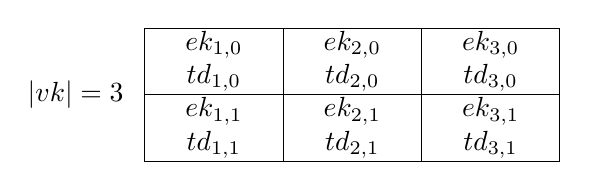
\begin{tikzpicture}
    \node [name=vk, textnode] {$|vk| = 3$}; 

    \node [name=ek10, rectanglenode, minimum width=5em, minimum height=2.4em, draw, 
        right of = vk, xshift=5em, yshift=1.2em] {$ek_{1,0}$\\$td_{1,0}$}; 
    \node [name=ek11, rectanglenode, minimum width=5em, minimum height=2.4em, draw, 
        right of = vk, xshift=5em, yshift=-1.2em] {$ek_{1,1}$\\$td_{1,1}$}; 

    \node [name=ek20, rectanglenode, minimum width=5em, minimum height=2.4em, draw, 
        right of = vk, xshift=10em, yshift=1.2em] {$ek_{2,0}$\\$td_{2,0}$}; 
    \node [name=ek21, rectanglenode, minimum width=5em, minimum height=2.4em, draw, 
        right of = vk, xshift=10em, yshift=-1.2em] {$ek_{2,1}$\\$td_{2,1}$}; 

    \node [name=ek30, rectanglenode, minimum width=5em, minimum height=2.4em, draw, 
        right of = vk, xshift=15em, yshift=1.2em] {$ek_{3,0}$\\$td_{3,0}$}; 
    \node [name=ek31, rectanglenode, minimum width=5em, minimum height=2.4em, draw, 
        right of = vk, xshift=15em, yshift=-1.2em] {$ek_{3,1}$\\$td_{3,1}$}; 
\end{tikzpicture}
\end{center}
\caption{$|vk|=3$时的求值公钥和求逆陷门生成图示}
\end{figure}


\begin{figure}[!hbtp]
\begin{minipage}[t]{0.5\linewidth}
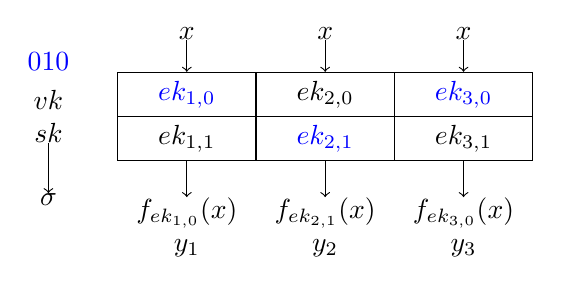
\begin{tikzpicture}
    \node [name=vk, textnode] {$vk$\\$sk$}; 

    \node [name=ek10, rectanglenode, minimum width=5em, minimum height=1.6em, draw, 
        right of = vk, xshift=5em, yshift=0.8em] {\blue{$ek_{1,0}$}}; 
    \node [name=ek11, rectanglenode, minimum width=5em, minimum height=1.6em, draw, 
        right of = vk, xshift=5em, yshift=-0.8em] {$ek_{1,1}$}; 

    \node [name=ek20, rectanglenode, minimum width=5em, minimum height=1.6em, draw, 
        right of = vk, xshift=10em, yshift=0.8em] {$ek_{2,0}$}; 
    \node [name=ek21, rectanglenode, minimum width=5em, minimum height=1.6em, draw, 
        right of = vk, xshift=10em, yshift=-0.8em] {\blue{$ek_{2,1}$}}; 

    \node [name=ek30, rectanglenode, minimum width=5em, minimum height=1.6em, draw, 
        right of = vk, xshift=15em, yshift=0.8em] {\blue{$ek_{3,0}$}}; 
    \node [name=ek31, rectanglenode, minimum width=5em, minimum height=1.6em, draw, 
        right of = vk, xshift=15em, yshift=-0.8em] {$ek_{3,1}$}; 

    \node [textnode, above of = vk, yshift=2em] {\blue{$010$}};   

    \node [textnode, name=x1, above of = ek10, yshift=2.2em] {$x$};
    \node [textnode, name=y1, below of = ek11, yshift=-3.2em] {$f_{ek_{1,0}}(x)$\\$y_1$}; 
    \draw (x1) edge[->] (ek10); 
    \draw (ek11) edge[->] (y1); 


    \node [textnode, name=x2, above of = ek20, yshift=2.2em] {$x$};
    \node [textnode, name=y2, below of = ek21, yshift=-3.2em] {$f_{ek_{2,1}}(x)$\\$y_2$}; 
    \draw (x2) edge[->] (ek20); 
    \draw (ek21) edge[->] (y2); 

    \node [textnode, name=x3, above of = ek30, yshift=2.2em] {$x$};
    \node [textnode, name=y3, below of = ek31, yshift=-3.2em] {$f_{ek_{3,0}}(x)$\\$y_3$}; 
    \draw (x3) edge[->] (ek30); 
    \draw (ek31) edge[->] (y3);    

    \node [textnode, name=signature, below of = vk, yshift=-3em] {$\sigma$}; 
    \draw (vk) edge[->] (signature);  
\end{tikzpicture}
\caption{$vk = 010$时的采样过程}
\end{minipage}
\begin{minipage}[t]{0.5\linewidth}
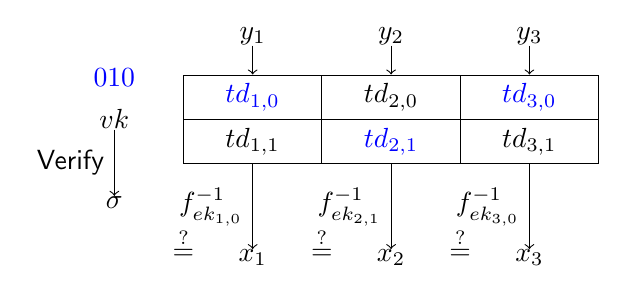
\begin{tikzpicture}
    \node [name=vk, textnode] {$vk$}; 

    \node [name=td10, rectanglenode, minimum width=5em, minimum height=1.6em, draw, 
        right of = vk, xshift=5em, yshift=0.8em] {\blue{$td_{1,0}$}}; 
    \node [name=td11, rectanglenode, minimum width=5em, minimum height=1.6em, draw, 
        right of = vk, xshift=5em, yshift=-0.8em] {$td_{1,1}$}; 

    \node [name=td20, rectanglenode, minimum width=5em, minimum height=1.6em, draw, 
        right of = vk, xshift=10em, yshift=0.8em] {$td_{2,0}$}; 
    \node [name=td21, rectanglenode, minimum width=5em, minimum height=1.6em, draw, 
        right of = vk, xshift=10em, yshift=-0.8em] {\blue{$td_{2,1}$}}; 

    \node [name=td30, rectanglenode, minimum width=5em, minimum height=1.6em, draw, 
        right of = vk, xshift=15em, yshift=0.8em] {\blue{$td_{3,0}$}}; 
    \node [name=td31, rectanglenode, minimum width=5em, minimum height=1.6em, draw, 
        right of = vk, xshift=15em, yshift=-0.8em] {$td_{3,1}$}; 

    \node [textnode, name=signature, below of = vk, yshift=-3em] {$\sigma$};
    \node [textnode, name=y1, above of = td10, yshift=2.2em] {$y_1$};
    \node [textnode, name=y2, above of = td20, yshift=2.2em] {$y_2$};
    \node [textnode, name=y3, above of = td30, yshift=2.2em] {$y_3$};

    \draw (vk) edge[->] node[left]{$\mathsf{Verify}$} (signature); 

    \node [textnode, above of = vk, yshift=1.5em] {\blue{$010$}};   

    \node [textnode, name=x1, below of = td11, yshift=-4.2em] {$x_1$}; 
    \draw (y1) edge[->] (td10); 
    \draw (td11) edge[->] node[left]{$f_{ek_{1,0}}^{-1}$} (x1); 
    \node [textnode, left of = x1, xshift=-2.5em, yshift=0.5em] {$\stackrel{?}{=}$}; 

    \node [textnode, name=x2, below of = td21, yshift=-4.2em] {$x_2$}; 
    \draw (y2) edge[->] (td20); 
    \draw (td21) edge[->] node[left]{$f_{ek_{2,1}}^{-1}$} (x2); 
    \node [textnode, left of = x2, xshift=-2.5em, yshift=0.5em] {$\stackrel{?}{=}$}; 

    \node [textnode, name=x3, below of = td31, yshift=-4.2em] {$x_3$}; 
    \draw (y3) edge[->] (td30); 
    \draw (td31) edge[->] node[left]{$f_{ek_{3,0}}^{-1}$} (x3); 
    \node [textnode, left of = x3, xshift=-2.5em, yshift=0.5em] {$\stackrel{?}{=}$};    
\end{tikzpicture}
\caption{$vk = 010$时的求逆过程}
\end{minipage}
\end{figure}


构造的正确性显然, 构造的以下三个特性使得归约算法能够成功模拟$\mathcal{O}_\mathsf{inv}$.
\begin{itemize}
    \item $\mathsf{R}_{ek}$是单射的并且$y_1||\dots||y_n$是对原像$x$的$n$重冗余求值. 
    \item $vk$是求值公钥的选择比特向量. 
    \item 利用OTS的sEUF-CMA安全性, $vk$在计算意义下绑定了$(y_1, \dots, y_n)$.  
\end{itemize} 

\begin{theorem}
    如果OTS是sEUF-CMA安全的, 并且$\mathcal{F}$是$\mathcal{U}_n$相关积单向的, 那么上述二元关系的构造满足自适应单向性.
\end{theorem}

\begin{proof}
证明通过以下游戏序列完成. 
\begin{trivlist}
\item $\text{Game}_0$: 对应真实的ATDR自适应单向性安全试验. 令$y^* = (vk^*, y_1^*||\dots||y_n^*, \sigma^*)$是挑战的像. 

\item $\text{Game}_1$: 与$\text{Game}_0$相同, 唯一的区别是挑战者对于求逆询问$y = (vk^*, y_1||\dots||y_n, \sigma)$直接返回$\bot$. 
应答的合理性分情况解释如下:
\begin{enumerate}
    \item $(y_1||\dots||y_v, \sigma) = (y_1^*||\dots||y_v^*, \sigma^*)$: 禁询点
    \item $(y_1||\dots||y_v, \sigma) \neq (y_1^*||\dots||y_v^*, \sigma^*)$: 构成OTS的存在性伪造
\end{enumerate} 
记敌手发起第二种类型求逆询问的事件为$F$, 那么利用Difference Lemma可以证明$|\Pr[S_1] - \Pr[S_0]| \leq \Pr[F]$, 
而基于OTS的sEUF-CMA安全性, 可以推出$\Pr[F] \leq \mathsf{negl}(\kappa)$, 从而$|\Pr[S_1] - \Pr[S_0]| \leq \mathsf{negl}(\kappa)$. 
\end{trivlist}

\begin{claim}
如果$\mathcal{F}$是$\mathcal{U}_t$相关积安全的, 那么对于任意的PPT敌手均有$\Pr[S_1] = \mathsf{negl}(\kappa)$. 
\end{claim}

\begin{proof}
论证通过单一归约完成. 假设存在PPT的敌手$\mathcal{A}$在$\text{Game}_1$中的优势不可忽略, 
那么尝试构造PPT算法$\mathcal{B}$, 通过黑盒调用$\mathcal{A}$的能力打破CP-TDF相对$\mathcal{U}_n$的相关积单向性. 
$\mathcal{B}$的CP-TDF挑战是公开参数$pp_\text{cptdf}$, 
求值公钥$(ek_1, \dots, ek_n)$和像$(y_1^*, \dots, y_n^*)$, 
其中$y_i^* \leftarrow f_{ek_i}(x^*)$, $x^* \sample X$. 
$\mathcal{B}$并不知晓$x^*$, 其攻击目标是求解$x^*$. 

\begin{figure}[!htbp]
\begin{center}
\begin{tikzpicture}
\node [textnode, name=vk, color=red] {$010$}; 

\node [textnode, name=ek1, right of = ek0, xshift=5em] {$ek_1$}; 
\node [textnode, name=x1, above of = ek1, yshift=2em, color=gray] {$x^*$}; 
\node [textnode, name=y1, below of = ek1, yshift=-2em] {$y_1^*$};
\draw (x1) edge[->] (ek1); 
\draw (ek1) edge[->] (y1); 

\node [textnode, name=ek2, right of = ek1, xshift=5em] {$ek_2$}; 
\node [textnode, name=x2, above of = ek2, yshift=2em, color=gray] {$x^*$}; 
\node [textnode, name=y2, below of = ek2, yshift=-2em] {$y_2^*$};
\draw (x2) edge[->] (ek2); 
\draw (ek2) edge[->] (y2); 

\node [textnode, name=ek3, right of = ek2, xshift=5em] {$ek_3$}; 
\node [textnode, name=x3, above of = ek3, yshift=2em, color=gray] {$x^*$}; 
\node [textnode, name=y3, below of = ek3, yshift=-2em] {$y_3^*$};
\draw (x3) edge[->] (ek3); 
\draw (ek3) edge[->] (y3); 
\end{tikzpicture}
\end{center}
\caption{$n=3$时$\mathcal{B}$的CP-TDF挑战实例}
\end{figure}
 
$\mathcal{B}$(扮演挑战者)与$\mathcal{A}$在$\text{Game}_1$中交互如下: 
\begin{itemize}
\item 初始化: $\mathcal{B}$运行$pp_\text{ots} \leftarrow \text{OTS}.\mathsf{Setup}(1^\kappa)$, 
	生成$(vk^*, sk^*) \leftarrow \text{OTS}.\mathsf{KeyGen}(pp_\text{ots})$. 
   	令$b_i^*$是$vk^*$的第$i$比特, $\mathcal{B}$进行如下操作: 
	\begin{enumerate}
    	\item 对$i \in [n]$设定$\red{ek_{i,b_i^*}} := ek_i$.
    	\item 对$i \in [v]$计算$(\blue{ek_{i, 1-b_i^*}, td_{i,1-b_i^*}}) \leftarrow \mathcal{F}.\mathsf{KeyGen}(pp_\text{cptdf})$.
	\end{enumerate}
	$\mathcal{B}$发送$pp = (pp_\text{cptdf}, pp_\text{ots})$和$ek = (ek_{1,0}, ek_{1,1}, \dots, ek_{n,0}, ek_{n,1})$给$\mathcal{A}$. 

\begin{figure}[!htbp]
\begin{center}
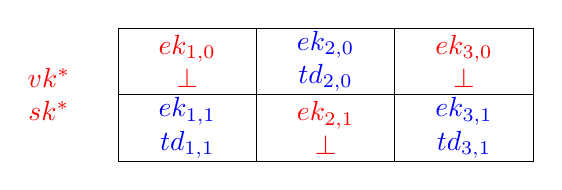
\begin{tikzpicture}
    \node [name=vk, textnode] {\red{$vk^*$}\\\red{$sk^*$}}; 

    \node [name=ek10, rectanglenode, minimum width=5em, minimum height=2.4em, draw, 
        right of = vk, xshift=5em, yshift=1.2em] {\red{$ek_{1,0}$}\\\red{$\bot$}}; 
    \node [name=ek21, rectanglenode, minimum width=5em, minimum height=2.4em, draw, 
        right of = vk, xshift=10em, yshift=-1.2em] {\red{$ek_{2,1}$}\\\red{$\bot$}}; 
    \node [name=ek30, rectanglenode, minimum width=5em, minimum height=2.4em, draw, 
        right of = vk, xshift=15em, yshift=1.2em] {\red{$ek_{3,0}$}\\\red{$\bot$}}; 

    \node [name=ek11, rectanglenode, minimum width=5em, minimum height=2.4em, draw, 
        right of = vk, xshift=5em, yshift=-1.2em] {\blue{$ek_{1,1}$}\\\blue{$td_{1,1}$}}; 
    \node [name=ek20, rectanglenode, minimum width=5em, minimum height=2.4em, draw, 
        right of = vk, xshift=10em, yshift=1.2em] {\blue{$ek_{2,0}$}\\\blue{$td_{2,0}$}}; 
    \node [name=ek31, rectanglenode, minimum width=5em, minimum height=2.4em, draw, 
        right of = vk, xshift=15em, yshift=-1.2em] {\blue{$ek_{3,1}$}\\\blue{$td_{3,1}$}}; 
\end{tikzpicture}
\end{center}
\caption{$|vk|=010$时归约算法设定求值公钥和求逆陷门的过程图示}
\end{figure}

\item 挑战: $\mathcal{B}$计算$\sigma^* \leftarrow \text{OTS}.\mathsf{Sign}(sk^*, (y_1^*, \cdots, y_n^*))$, 
	发送$(vk^*, y_1^*, \cdots, y_n^*, \sigma^*)$给$\mathcal{A}$作为挑战. 

\item 求逆询问: 对于求逆询问$y = (vk, y_1||\dots||y_v, \sigma)$, $\mathcal{B}$应答如下:   
\begin{enumerate}
    \item $vk = vk^*$: 直接返回$\bot$. 

    \item $vk \neq vk^*$: 必然存在$\exists j \in [n]$ s.t. $b_j \neq b_j^*$且$y_j = f_{{ek_j, b_j}}(x)$, 其中$x$是未知原像. 
    此时, $\mathcal{B}$拥有关于$ek_{j,b_j}$的求逆陷门$td_{j,b_j}$, $\mathcal{B}$可计算$x \leftarrow f_{ek_j, b_j}^{-1}(y_j)$
	\begin{itemize}
    	\item 如果$y_i = f_{ek_{i,b_i}}(x)$对所有的$i \neq j$也均成立, 那么返回$x$, 否则返回$\bot$. 
	\end{itemize}
\end{enumerate} 
由$\mathcal{F}$的单射性可知, $\mathcal{B}$完美的模拟了$\text{Game}_1$中的$\mathcal{O}_\mathsf{inv}$应答. 

\begin{figure}[!htbp]
\begin{center}
\begin{tikzpicture}
    \node [name=vk, textnode] {\red{$vk$}}; 

    \node [name=ek10, rectanglenode, minimum width=5em, minimum height=2.4em, draw, 
        right of = vk, xshift=5em, yshift=1.2em] {\red{$ek_{1,0}$}\\\red{$\bot$}};
    \node [name=ek11, rectanglenode, minimum width=5em, minimum height=2.4em, draw, 
        right of = vk, xshift=5em, yshift=-1.2em] {\blue{$ek_{1,1}$}\\\blue{$td_{1,1}$}}; 

    \node [name=ek20, rectanglenode, minimum width=5em, minimum height=2.4em, draw, 
        right of = vk, xshift=10em, yshift=1.2em] {\blue{$ek_{2,0}$}\\\blue{$td_{2,0}$}};  
    \node [name=ek21, rectanglenode, minimum width=5em, minimum height=2.4em, draw, 
        right of = vk, xshift=10em, yshift=-1.2em] {\red{$ek_{2,1}$}\\\red{$\bot$}}; 

    \node [name=ek30, rectanglenode, minimum width=5em, minimum height=2.4em, draw, 
        right of = vk, xshift=15em, yshift=1.2em] {\red{$ek_{3,0}$}\\\red{$\bot$}}; 
    \node [name=ek31, rectanglenode, minimum width=5em, minimum height=2.4em, draw, 
        right of = vk, xshift=15em, yshift=-1.2em] {\blue{$ek_{3,1}$}\\\blue{$td_{3,1}$}}; 

    \node [name=x1, above of = ek10, yshift=1.3em] {\gray{$x$}};
    \node [name=y1, below of = ek11, yshift=-1.3em] {\gray{$y_1$}};
    \draw (x1) edge[->] (ek10);
    \draw (ek11) edge[->] (y1); 

    \node [name=x2, above of = ek20, yshift=1.3em] {\gray{$x$}};
    \node [name=y2, below of = ek21, yshift=-1.3em] {\gray{$y_2$}};

    \node [name=x3, above of = ek30, yshift=1.3em] {\gray{$x$}};
    \node [name=y3, below of = ek31, yshift=-1.3em] {\gray{$y_3$}};
    \draw (x3) edge[->] (ek30);
    \draw (ek31) edge[->] (y3); 

    \draw (x2) edge[->] (ek20);
    \draw (ek21) edge[->] (y2); 

    \node [name=signature, below of = vk, yshift=-2.5em] {$\sigma$};
    \draw (vk) edge[->] node[left, yshift=1em] {$\mathsf{Verify}$} (signature); 

    \node [rectanglenode, minimum width=5em, minimum height=2.4em, draw, 
        right of = ekhat, xshift=10em, yshift=1.2em, color=blue, thick] {}; 
    \draw (y2) edge[->, thick, color=blue] (ek21);
    \draw (ek20) edge[->, thick, color=blue] (x2); 

    \node [textnode, left of = y0, xshift=-1em, yshift=1.5em] {$\stackrel{?}{=}$}; 
    \node [textnode, left of = y1, xshift=-1em, yshift=1.5em] {$\stackrel{?}{=}$}; 
    \node [textnode, left of = y3, xshift=-1em, yshift=1.5em] {$\stackrel{?}{=}$}; 
\end{tikzpicture}
\end{center}
\caption{$vk=010$时归约算法求逆过程图示}
\end{figure}

\item 求解: $\mathcal{A}$输出$x$作为$\text{Game}_1$中ATDF的挑战应答, $\mathcal{B}$将$x$转发给CP-TDF的挑战者. 
\end{itemize}
容易验证, $\mathcal{B}$的优势与$\mathcal{A}$的优势相同. 断言得证. \qed
\end{proof}
综上, 定理得证! \qed
\end{proof}

\section*{小结}
Rosen和Regev~\cite{RS-TCC-2009}证明了CP-TDF与LTDF之间存在黑盒分离, Kiltz、Mohassel和O'Neill~\cite{KMO-EUROCRYPT-2010}证明了ATDF与CP-TDF之间也存在黑盒分离. 
因此, 在黑盒的意义下, ATDF和ATDR是目前单向函数类中构造CCA-KEM所需的最弱组件. 
\begin{figure}
\begin{center}
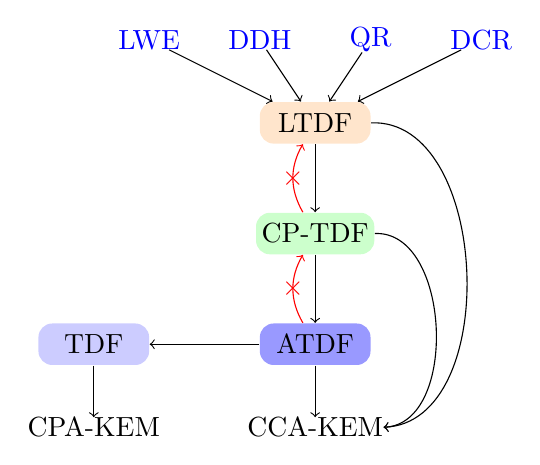
\begin{tikzpicture}
    \node [name=TDF, roundnode, draw=none, fill=blue!20, minimum width=4em] {TDF};
    \node [name=CPAKEM, textnode, below of = TDF, yshift=-3em] {CPA-KEM}; 
    \draw (TDF) edge[->] (CPAKEM);

    \node [name=ATDF, roundnode, right of = TDF, xshift=8em, draw=none, fill=blue!40, minimum width=4em] {ATDF};
    \node [name=CCAKEM, textnode, below of = ATDF, yshift=-3em] {CCA-KEM}; 
    \draw (ATDF) edge[->] (CCAKEM);
    \draw (ATDF) edge[->] (TDF);

    \node [name=CPTDF, roundnode, above of = ATDF, yshift=4em, draw=none, fill=green!20] {CP-TDF};
    \node [name=LTDF, roundnode, above of = CPTDF, yshift=4em, draw=none, fill=orange!20, minimum width=4em] {LTDF};
    \draw (LTDF) edge[->, bend left=90] (CCAKEM);
    \draw (CPTDF) edge[->, bend left=90] (CCAKEM);
    \draw (ATDF) edge[color=red, ->, bend right=-30] node {$\times$} (CPTDF);
    \draw (CPTDF) edge[color=red, ->, bend right=-30] node {$\times$} (LTDF);
    \draw (LTDF) edge[->, thin] (CPTDF);
    \draw (CPTDF) edge[->, thin] (ATDF);

    \node [name=LWE, above of = LTDF, xshift=-6em, yshift=3em, textnode, color=blue] {LWE};
    \node [name=DDH, above of = LTDF, xshift=-2em, yshift=3em, textnode, color=blue] {DDH};
    \node [name=QR, above of = LTDF, xshift=2em, yshift=3em, textnode, color=blue] {QR};
    \node [name=DCR, above of = LTDF, xshift=6em, yshift=3em, textnode, color=blue] {DCR};

    \draw (LWE) edge[->] (LTDF);
    \draw (DDH) edge[->] (LTDF);
    \draw (QR) edge[->] (LTDF);
    \draw (DCR) edge[->] (LTDF);
\end{tikzpicture}
\end{center}
\caption{各类单向函数之间的蕴含关系}
\end{figure}

% \begin{frame}{How to expand the DEM key?}
% \uncover<1->{
% \begin{trivlist}
%     \item $K = \text{Img}(\mathsf{hc})$. $\mathsf{GL}: X \rightarrow \{0,1\}$ is generic but yields 1-bit key. 
% \end{trivlist}

% \begin{center}
%     \emph{How to expand?}
% \end{center}
% }
% \vspace{-1em}

% \begin{itemize}
% \uncover<2->{
% \item multiple sampling
%     \begin{center}
%         $x_i \sample X$, $c_i \leftarrow f(x_i)$, $k_i \leftarrow \mathsf{hc}(x_i)$
%     \end{center}
%     \begin{remarkblock}
%     \begin{center}
%         linear expansion of ciphertext and easily malleable $\leadsto$ vulnerable to CCA attack
%     \end{center}
%     \end{remarkblock}
% }

% \uncover<3->{
% \item $\mathsf{hc}(\cdot)$ with multi-bits outputs
%     \begin{itemize}
%         \item rely on decisional assumptions
%         \item iterating $f$ when $f$ is permutation
%         \item differing-input indistinguishability obfuscation
%     \end{itemize}
%     \begin{center}
%         \red{rely on stronger assumption}
%     \end{center}
% }
% \end{itemize}
% \end{frame}








\section{哈希证明系统类}
\begin{center}
	一阴一阳之谓道, 继之者善也, 成之者性也.\\
                \hfill --- 《易经 · 系辞上》
\end{center}

1998年, Cramer和Shoup~\cite{CS-CRYPTO-1998}基于判定性Diffie-Hellman问题构造出首个标准模型下高效的公钥加密方案, 成为CS98-PKE. 
2002年, Cramer和Shoup~\cite{CS-EUROCRYPT-2002}再度合作, 提出了哈希证明系统(HPS, hash proof system)的概念, 
给出了标准模型下构造CCA-secure PKE的全新范式, 完美的阐释了CS98-PKE的设计原理. 
在同一篇论文中, 作者还正式提出了KEM+DEM的公钥加密工作模式, 相比朴素混合加密更加现代、模块化. 
以下首先介绍HPS的定义和相关性质. 


\begin{definition}[哈希证明系统]
HPS包含以下多项式时间算法: 
\begin{itemize}
\item $\mathsf{Setup}(1^\kappa)$: 以安全参数$\kappa$为输入, 输出公开参数$pp = (\mathsf{H}, SK, PK, X, L, W, \Pi, \alpha)$, 
    其中$\mathsf{H}: SK \times X \rightarrow \Pi$是由私钥集合$SK$索引的一族带密钥哈希函数(keyed hash function), 
    $L$是定义在$X$上的$\mathcal{NP}$语言, $W$是对应的证据集合, $\alpha$是从私钥集合$SK$到公钥集合$PK$的投射函数. 

\item $\mathsf{KeyGen}(pp)$: 以公开参数$pp$为输入, 随机采样$sk \sample SK$, 计算$pk \leftarrow \alpha(sk)$, 输出$(pk, sk)$. 

\item $\mathsf{PrivEval}(sk, x)$: 以私钥$sk$和$x \in X$为输入, 输出$\pi = \mathsf{H}_{sk}(x)$. 

\item $\mathsf{PubEval}(pk, x, w)$: 以公钥$pk$、$x \in L$以及相应的$w$为输入, 输出$\pi = \mathsf{H}_{sk}(x)$, 其中$\alpha(sk) = pk$. 
\end{itemize}
\end{definition}

\begin{figure}[!htbp]
\begin{center}
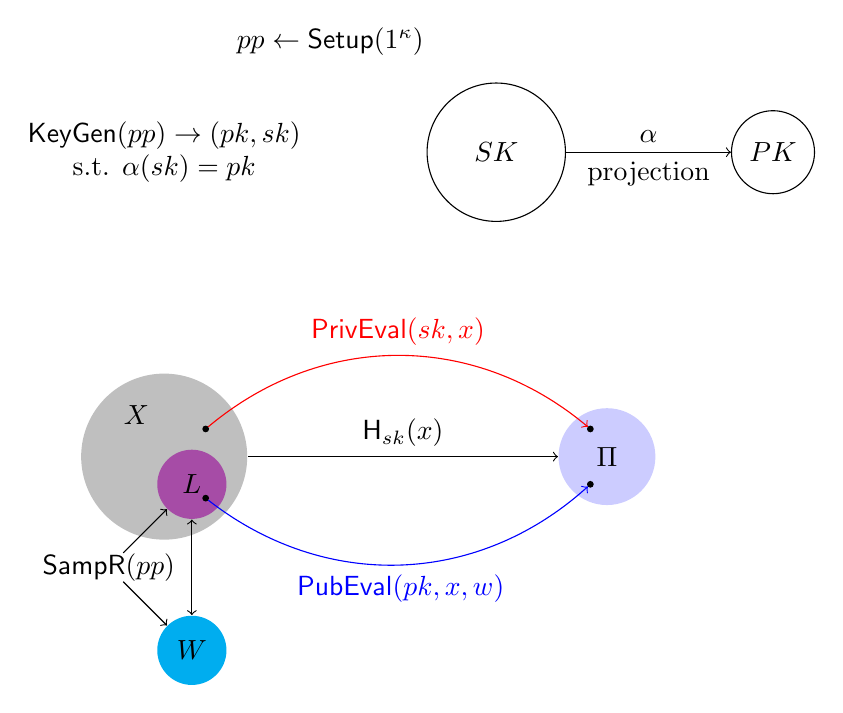
\begin{tikzpicture}
    \node[textnode, name=Setup] {$pp \leftarrow \mathsf{Setup}(1^\kappa)$}; 
    \node[textnode, name=KeyGen, below of=Setup, xshift=-6em, yshift=-4em] {$\mathsf{KeyGen}(pp) \rightarrow (pk, sk)$ \\s.t. $\alpha(sk) = pk$}; 
    \node[circlenode, name=SK, right of = KeyGen, xshift=12em, minimum size=5em] {$SK$};
    \node[circlenode, name=PK, right of = SK, xshift=10em, minimum size=3em] {$PK$};
    \draw (SK) edge[->] node[above] {$\alpha$} node[below] {projection} (PK);


    \node[circlenode, name = X, below of = Setup, xshift=-6em, yshift=-15em, draw=none, fill=gray!50, minimum size=6em] {};
    \node[textnode, above of = X, xshift=-1em, yshift=1.5em] {$X$}; 
    \node[circlenode, name = L, below of = X, xshift=1em, yshift=-1em, draw = none, fill=violet!70, minimum size=2.5em] {$L$};
    \node[circlenode, name = W, below of = L, yshift=-6em, draw=none, fill=cyan, minimum size=2.5em] {$W$};
    \node[textnode, name = SampR, below of = L, xshift=-3em, yshift=-3em] {$\mathsf{SampR}(pp)$};
    \draw (SampR) edge[->] (L);
    \draw (SampR) edge[->] (W); 
    \draw (L) edge[<->] (W); 

    \node[circlenode, name = Pi, right of = X, xshift=16em, draw=none, fill=blue!20, minimum size=3.5em] {$\Pi$};

    \draw (X) edge[->] node[above] {$\mathsf{H}_{sk}(x)$} (Pi); 

    \node[dotnode, name = x1, above of = X, xshift=1.5em, yshift=1em] {}; 
    \node[dotnode, name = y1, above of = Pi, xshift=-0.6em, yshift=1em] {}; 
    \draw (x1) edge[color=red, ->, bend left=40] node[above] {$\mathsf{PrivEval}(sk, x)$} (y1);

    \node[dotnode, name = x2, below of = X, xshift=1.5em, yshift=-1.5em] {}; 
    \node[dotnode, name = y2, above of = Pi, xshift=-0.6em, yshift=-1em] {}; 
    \draw (x2) edge[color=blue, ->, bend left=-40] node[below] {$\mathsf{PubEval}(pk, x, w)$} (y2);
\end{tikzpicture}
\end{center}
\caption{HPS示意图}
\end{figure}

HPS的定义围绕$L \subset X$展开, 引入了$\mathsf{KeyGen}$, $\mathsf{PrivEval}$和$\mathsf{PubEval}$这三个核心算法. 
以下性质刻画了哈希函数在输入$x \in L$上的行为, 用于保证上层密码方案的功能性.  
\begin{trivlist}
\item \textbf{投射性(Projectivity):} $\forall x \in L$, 函数值$\mathsf{H}_{sk}(x)$由$x$和私钥的投射$pk \leftarrow \alpha(sk)$完全确定.
\end{trivlist}

以下性质由弱到强刻画了哈希函数在输入$x \in X \backslash L$上的行为, 用于保证上层密码方案的安全性.  
% \begin{block}{Smooth: for $x^* \sample X \backslash L$}

\begin{trivlist}
\item \textbf{平滑性(Smooth):} $\mathsf{H}_{sk}(\cdot)$在输入$x \sample X \backslash L$时的输出与$\Pi$上的均匀分布统计接近, 即: 
\begin{equation*}
    (pk, \mathsf{H}_{sk}(x)) \approx_s (pk, \pi)
\end{equation*}
其中$(pk, sk) \leftarrow \mathsf{KeyGen}(pp)$, $\pi \sample \Pi$.   


\item \textbf{1-一致性(1-Universal):} $\mathsf{H}_{sk}(\cdot)$在任意输入的输出与$\Pi$上的均匀分布统计接近, 
    即$\forall x \in X \backslash L$, 有:
\begin{equation*}
    (pk, \mathsf{H}_{sk}(x)) \approx_s (pk, \pi)
\end{equation*}
其中$(pk, sk) \leftarrow \mathsf{KeyGen}(pp)$, $\pi \sample \Pi$. 

\item \textbf{2-一致性(2-Universal):} 在给定某点$x^* \in X \backslash L$哈希函数值的情形下, 
    $\mathsf{H}_{sk}(\cdot)$在任意输入的输出仍与$\Pi$上的均匀分布统计接近, 
    即$\forall x, x^* \in X \backslash L$且$x \neq x^*$, 有:
\begin{equation*}
    (pk, \mathsf{H}_{sk}(x^*), \mathsf{H}_{sk}(x)) \approx_s (pk, \mathsf{H}_{sk}(x^*), \pi)
\end{equation*}
其中$(pk, sk) \leftarrow \mathsf{KeyGen}(pp)$, $\pi \sample \Pi$. 
\end{trivlist}

\begin{note}
以上三条性质由弱到强. 
smooth性质同时建立在$sk \sample SK$和$x \sample X \backslash L$两根随机带上, 
1-universal性质仅建立在$sk \sample SK$一根随机带上, 
而2-universal性质则可解读为要求1-universal性质在随机带$sk \sample SK$有偏时(将$\mathsf{H}_{sk}(x^*)$理解为关于$sk$的泄漏)仍然成立. 
特别注意, 三条性质均刻画的是输入在语言外时哈希函数的行为.
\end{note}

\subsection{起源释疑}
相信很多读者在阅读HPS早期的文献时, 都会对这个范式的命名和引入动机感到疑惑. 
事实上, HPS是一类指定验证者的非交互式零知识证明系统(designated verifier NIZK), 
引入的动机来自以下的思考: Naor-Yung双重加密范式使用标准的NIZK来证明密文的合法性(well-formedness), 
然而密文的合法性并非一定是可公开验证的(public verifiable), 解密私钥$sk$的持有者可验证即可. 
指定可验证弱于公开可验证, 因此DV-NIZK的效率通常高于NIZK. 
想必Cramer和Shoup正是基于以上的思考, 引入了HPS, 目的是在标准模型下构造高效的CCA-secure PKE. 

\begin{figure}[!htbp]
\begin{center}
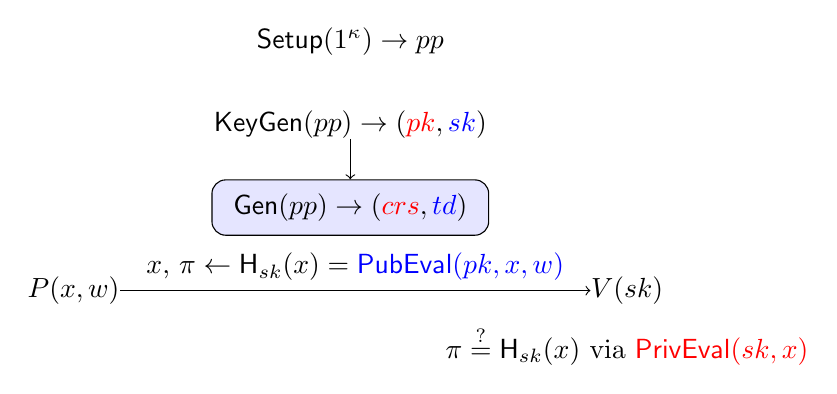
\begin{tikzpicture}
\node [textnode, name=Setup] {$\mathsf{Setup}(1^\kappa) \rightarrow pp$}; 
\node [textnode, name=HGen, below of = Setup, yshift=-3em] {$\mathsf{KeyGen}(pp) \rightarrow (\red{pk}, \blue{sk})$};
\node [roundnode, name=Gen, below of = HGen, fill=blue!10, yshift=-3em, minimum width=10em, minimum height=2em] 
{$\mathsf{Gen}(pp) \rightarrow (\red{crs}, \blue{td})$};
\draw (HGen) edge[->] (Gen);

\node [name=Prover, textnode, below of=Gen, xshift=-10em, yshift=-3em] {$P(x, w)$};
\node [name=Verifier, textnode, below of=Gen, xshift=10em, yshift=-3em] {$V(sk)$};  
\node [name=Check, textnode, below of=Verifier, yshift=-2em] 
{$\pi \stackrel{?}{=} \mathsf{H}_{sk}(x)$ via \red{$\mathsf{PrivEval}(sk, x)$}};   
\draw (Prover) edge[->] node[above] {$x$, $\pi \leftarrow \mathsf{H}_{sk}(x) = 
    \blue{\mathsf{PubEval}(pk, x, w)}$} (Verifier);
\end{tikzpicture}
\end{center}
\caption{从DV-NIZK的视角解析HPS}
\end{figure}

\begin{note}
上图解释了HPS的命名渊源, 其本质上是指定验证者零知识证明, 证明的形式是实例的哈希值, 故名\emph{哈希证明系统}. 
\end{note}

\begin{itemize}
\item DV-NIZK的完备性由$\mathsf{H}_{sk}(\cdot)$的投射性保证:
\begin{equation*}
    \forall x \in L, \mathsf{H}_{sk}(x) = \mathsf{PubEval}(pk, x, w)
\end{equation*}

\item DV-NIZK的合理性由1-universal性质保证$\forall x \notin L$, $\mathsf{H}_{sk}(x)$随机分布, 
    即使拥有无限计算能力的证明者$P^*$也无法预测, 因此通过验证的概率可忽略. 
    2-universal性质则保证了更强的合理性, 即敌手在看到一个No实例的有效证明后, 也无法为一个新的No实例生成有效证明.    

\item DV-NIZK的零知识性是显然且平凡的: 指定验证者拥有私钥, 
    因此可以对任意的$x \in L$(甚至是$x \in X$)生成正确的证明 
\end{itemize}
此外, 证明系统是有效的, 即证明者在拥有证据时可以高效计算出实例的证明, 这对于基于HPS密码方案的功能性至关重要. 


\subsection{HPS的构造}
我们首先以针对$L_\text{DDH}$语言的HPS构造为例, 获得对HPS设计方式的直观认识. 
令$(\mathbb{G}, p, g)$是算法$\mathsf{GroupGen}(1^\kappa)$的输出, 
其中$\mathbb{G}$是阶为素数$p$的群, $g$是生成元. 随机选取$\mathbb{G}$中的两个生成元$g_1, g_2$. 
令$pp = (\mathbb{G}, p, g_1, g_2)$是公开参数, 定义由$pp$索引的$\mathcal{NP}$语言如下:  
\begin{equation*}
    L_\text{DDH} = \{(x_1, x_2) \in X: \exists w \in W \text{~s.t.~} x_1 = g_1^w, x_2 = g_2^w\}
\end{equation*}
其中$X = \mathbb{G} \times \mathbb{G}$, $W = \mathbb{Z}_p$. 

容易验证, 语言中的元素是DH对, 语言外的元素是非DH对, $(x_1, x_2) \sample L_\text{DDH}$.  
DDH假设蕴含$L \subset X$上的SMP困难问题成立, 即: 
\begin{itemize}
    \item $U_L \approx_c U_X$: 随机DH对与$X$中的随机二元组计算不可区分

    \item 由于$|L|/|X| = 1/p = \mathsf{negl}(\kappa)$, $L$在$X$中稀疏, 
        所以可以进一步得到$U_L \approx_c U_{X \backslash L}$: 随机DH对与随机非DH对计算不可区分
\end{itemize}

\begin{construction}[$L_\text{DDH}$语言的HPS构造]\label{construction:HPS-for-DDH}
$L_\text{DDH}$的HPS构造如下, 如图~\ref{figure:HPS-DH}所示:
\begin{itemize}
\item $\mathsf{Setup}(1^\kappa)$: 以安全参数$\kappa$为输入, 输出公开参数$pp = (\mathbb{G}, p, g_1, g_2)$. 
    $pp$还包括了对$SK = \mathbb{Z}_p \times \mathbb{Z}_p$, $PK = \mathbb{G}$, $L_\text{DDH}$, 
    $X = \mathbb{G} \times \mathbb{G}$和$W = \mathbb{Z}_p$的描述.   

\item $\mathsf{KeyGen}(pp)$: 以公开参数$pp$为输入, 随机采样$sk \sample \mathbb{Z}_p^2$, 
    计算$pk \leftarrow \alpha(sk) = g_1^{sk_1} g_2^{sk_2}$, 输出$(pk, sk)$. 

\item $\mathsf{PrivEval}(sk, x)$: 以私钥$sk$和$x \in X$为输入, 输出$\pi = \mathsf{H}_{sk}(x) = x_1^{sk_1} x_2^{sk_2}$. 

\item $\mathsf{PubEval}(pk, x, w)$: 以公钥$pk$、$x \in L_\text{DDH}$以及相应的$w$为输入, 输出$\pi = pk^w$, 其中$\alpha(sk) = pk$. 
    以下等式说明了公开求值算法的正确性:
    \begin{equation*}
        pk^w = (g_1^{sk_1} g_2^{sk_2})^w = x_1^{sk_1} x_2^{sk_2} = \mathsf{H}_{sk}(x)
    \end{equation*}
\end{itemize}
\end{construction}

\begin{figure}[!htbp]
\begin{center}
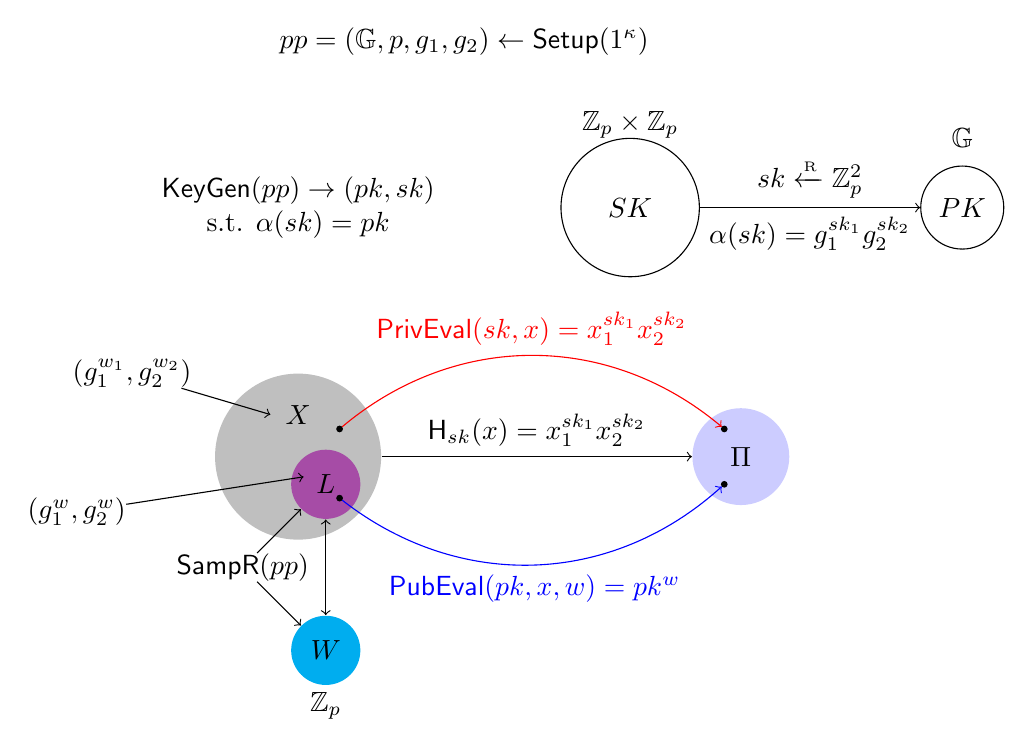
\begin{tikzpicture}
    \node[textnode, name=Setup] {$pp = (\mathbb{G}, p, g_1, g_2) \leftarrow \mathsf{Setup}(1^\kappa)$}; 
    \node[textnode, name=KeyGen, below of=Setup, xshift=-6em, yshift=-6em] {$\mathsf{KeyGen}(pp) \rightarrow (pk, sk)$ \\s.t. $\alpha(sk) = pk$}; 
    \node[circlenode, name=SK, right of = KeyGen, xshift=12em, minimum size=5em] {$SK$};
    \node[textnode, above of = SK, yshift=3em] {$\mathbb{Z}_p \times \mathbb{Z}_p$}; 
    \node[circlenode, name=PK, right of = SK, xshift=12em, minimum size=3em] {$PK$};
    \node[textnode, above of = PK, yshift=2.5em] {$\mathbb{G}$}; 
    \draw (SK) edge[->] node[above] {$sk \sample \mathbb{Z}_p^2$} node[below] {$\alpha(sk) = g_1^{sk_1} g_2^{sk_2}$} (PK);


    \node[circlenode, name = X, below of = Setup, xshift=-6em, yshift=-15em, draw=none, fill=gray!50, minimum size=6em] {};
    \node[textnode, above of = X, xshift=0em, yshift=1.5em] {$X$}; 

    \node[textnode, name=random-tuple, left of = X, xshift=-6em, yshift=3em] {$(g_1^{w_1}, g_2^{w_2})$}; 
    \draw (random-tuple) edge[->] ($(X.north)+(-1em, -1.5em)$); 

    \node[circlenode, name = L, below of = X, xshift=1em, yshift=-1em, draw = none, fill=violet!70, minimum size=2.5em] {$L$};
    \node[textnode, name=DH-tuple, left of = L, xshift=-9em, yshift=-1em] {$(g_1^w, g_2^w)$}; 
    \draw (DH-tuple) edge[->] ($(L.north)+(-0.8em, -1em)$); 

    \node[circlenode, name = W, below of = L, yshift=-6em, draw=none, fill=cyan, minimum size=2.5em] {$W$};
    \node[textnode, below of = W, yshift=-2em] {$\mathbb{Z}_p$}; 
    \node[textnode, name = SampR, below of = L, xshift=-3em, yshift=-3em] {$\mathsf{SampR}(pp)$};
    \draw (SampR) edge[->] (L);
    \draw (SampR) edge[->] (W); 
    \draw (L) edge[<->] (W); 

    \node[circlenode, name = Pi, right of = X, xshift=16em, draw=none, fill=blue!20, minimum size=3.5em] {$\Pi$};

    \draw (X) edge[->] node[above] {$\mathsf{H}_{sk}(x) = x_1^{sk_1} x_2^{sk_2}$} (Pi); 

    \node[dotnode, name = x1, above of = X, xshift=1.5em, yshift=1em] {}; 
    \node[dotnode, name = y1, above of = Pi, xshift=-0.6em, yshift=1em] {}; 
    \draw (x1) edge[color=red, ->, bend left=40] node[above] {$\mathsf{PrivEval}(sk, x) = x_1^{sk_1} x_2^{sk_2}$} (y1);

    \node[dotnode, name = x2, below of = X, xshift=1.5em, yshift=-1.5em] {}; 
    \node[dotnode, name = y2, above of = Pi, xshift=-0.6em, yshift=-1em] {}; 
    \draw (x2) edge[color=blue, ->, bend left=-40] node[below] {$\mathsf{PubEval}(pk, x, w) = pk^w$} (y2);
\end{tikzpicture}
\end{center}
\caption{$L_\text{DDH}$的HPS}\label{figure:HPS-DH}
\end{figure}

\begin{lemma}
以上关于$L_\text{DDH}$的HPS满足1-universal性质. 
\end{lemma}

\begin{proof}
证明的目标是
\begin{equation*}
    \forall x \in X \backslash L, (pk, \mathsf{H}_{sk}(x)) \approx_s (pk, \pi)
\end{equation*}
其中$(pk, sk) \leftarrow \mathsf{KeyGen}(pp)$, $\pi \sample \Pi$. 


首先固定$x = (x_1 = g_1^{w_1}, x_2 = g_2^{w_2}) \in X \backslash L$, 其中$w_1 \neq w_2$. 
将左式表示为关于$sk$函数的形式:
\begin{equation*}
    (pk, \mathsf{H}_{sk}(x)) = f_{g_1, g_2, x_1, x_2}(sk_1,sk_2) := (g_1^{sk_1}g_2^{sk_2}, x_1^{sk_1}x_2^{sk_2})
\end{equation*}
用矩阵的形式描述函数作用过程:
\begin{displaymath}
\left(\begin{array}{cc}
g_1 & g_2\\
g_1^{w_1} & g_2^{w_2}
\end{array} \right)
\left(\begin{array}{c}
sk_1\\
sk_2
\end{array} \right) 
= 
\left(\begin{array}{c}
pk\\
\mathsf{H}_{sk}(x)
\end{array} \right)
\end{displaymath} 
令$g_2 = g_1^\beta$, 其中$\beta \in \mathbb{Z}_p$, 将最左边矩阵进行等价变形: 
\begin{displaymath}
\left(\begin{array}{cc}
g_1 & g_2\\
g_1^{w_1} & g_2^{w_2}
\end{array} \right) = 
\left(\begin{array}{cc}
g_1 & g_1^{\beta}\\
g_1^{w_1} & g_1^{w_2\beta}
\end{array} \right) = 
g_1
\underbrace{
\left(\begin{array}{cc}
1 & \beta\\
w_1 & w_2\beta
\end{array} \right)
}_{M} 
\end{displaymath}
$\textup{det}(M) = \beta(w_1-w_2)$ $\Rightarrow$ $M$满秩 $\Rightarrow$ 
$f$单射. 又由于函数的定义域和值域大小相等, 最终得出:  
\begin{displaymath}
\underbrace{
\left(\begin{array}{cc}
g_1 & g_2\\
g_1^{w_1} & g_2^{w_2}
\end{array} \right)
}_{\text{full rank~} 2 \times 2} 
\underbrace{
\left(\begin{array}{c}
sk_1\\
sk_2
\end{array} \right) 
}_{\text{~uniform over~} \mathbb{Z}_p^2}= 
\underbrace{
\left(\begin{array}{c}
pk\\
\mathsf{H}_{sk}(x)
\end{array} \right)
}_{\text{uniform over~} \mathbb{G}^2}
\end{displaymath} 
从而1-universal性质得证! \qed
\end{proof}

\begin{remark}
HPS并不一定要求$L \subseteq X$之上一定存在SMP问题, 但只有当$L \subseteq X$之上存在SMP问题时, 相应的HPS有密码学意义. 
这是因为HPS中所有关于哈希函数的性质均是针对输入在语言外时定义的, 只有当SMP问题存在时, 才可以间接刻画出哈希函数在输入在语言内时的行为. 
\end{remark}

HPS存在两个局限: 
\begin{itemize}
    \item 证明只支持私密验证, 不满足公开验证性
    \item 证明的表达能力有限, 目前仅能对证明群中的子群成员归属问题, 尚未知能否延伸到任意的NP语言. 
\end{itemize}
在很多具体的零知识证明应用场合, 公开验证性和强大的表达能力均不是必须, 因此用标准的零知识证明系统有大材小用之嫌, 
哈希证明系统可以做的更快更好, 其中效率的优势恰恰源自局限. 以下展示如何基于HPS设计IND-CPA和IND-CCA的KEM方案. 


\subsection{基于HPS构造IND-CPA KEM}
作为暖场应用, 我们首先介绍如何基于HPS构造CPA安全的KEM. 设计的思路如下: 
\begin{itemize}
\item 发送方扮演HPS中的证明者, 选择$L$中的随机实例$x$作为密文$c$, 利用公钥$pk$和相应的证据$w$计算其哈希证明$\pi$作为会话密钥$k$. 

\item 接收方扮演HPS中的验证者, 使用私钥$sk$计算$x$的哈希证明以恢复会话密钥$k$. 
\end{itemize}

\begin{construction}[基于HPS的CPA安全KEM]\label{construction:CPA-KEM-from-HPS}
从smooth的HPS出发, 构造CPA安全的KEM如下: 
\begin{itemize}
\item $\mathsf{Setup}(\kappa)$: 运行$pp \leftarrow \text{HPS}.\mathsf{Setup}(1^\kappa)$, 
    输出$pp = (\mathsf{H}, SK, PK, X, L, W, \Pi, \alpha)$作为公开参数, 其中$X$作为密文空间, $\Pi$作为会话密钥空间. 

\item $\mathsf{KeyGen}(pp)$: 运行$(pk, sk) \leftarrow \text{HPS}.\mathsf{KeyGen}(pp)$, 输出公钥$pk$和私钥$sk$. 

\item $\mathsf{Encaps}(pk; r)$: 以公钥$pk$和随机数$r$为输入, 执行如下步骤: 
\begin{enumerate}
    \item 运行$(x, w) \leftarrow \mathsf{SampR}(r)$生成随机实例和相应的证据;
    \item 通过$\text{HPS}.\mathsf{PubEval}(pk, x, w)$计算实例$x$的哈希证明$\pi \leftarrow \mathsf{H}_{sk}(x)$; 
    \item 输出实例$x$作为密文$c$, 输出哈希证明$\pi$作为会话密钥$k$. 
\end{enumerate}

\item $\mathsf{Decaps}(sk, c)$: 以私钥$sk$和密文$c$为输入, 通过$\text{HPS}.\mathsf{PrivEval}(sk, c)$
    计算$c$的哈希证明$\pi \leftarrow \mathsf{H}_{sk}(x)$以恢复会话密钥$k$. 
\end{itemize}
\end{construction} 

KEM方案的正确性有HPS的完备性保证. 安全性由如下定理保证. 

\begin{theorem}
如果$L \subseteq X$上的SMP困难问题成立, 那么构造~\ref{construction:CPA-KEM-from-HPS}中的KEM是IND-CPA安全的. 
\end{theorem}

\begin{proof}
我们将通过游戏序列组织证明. 游戏序列的编排次序由如下证明思路指引:  
\begin{itemize}
    \item 将诚实生成的密文分布$x \sample L$切换为$x \sample X \backslash L$
    \item 论证当$x \sample X \backslash L$时, $(pk, \pi = \mathsf{H}_{sk}(x))$的分布与$(pk, \pi \sample \Pi)$统计接近. 
\end{itemize} 

\begin{trivlist}
\item $\text{Game}_0$: 对应真实的游戏, 其中挑战密文$x^* \sample L$, 计算会话密钥的方式是对$\mathsf{H}_{sk}(x^*)$进行公开求值
\begin{itemize}
    \item 初始化: $\mathcal{CH}$计算$pp \leftarrow \text{HPS}.\mathsf{Setup}(1^\kappa)$, 
        $(pk, sk) \leftarrow \text{HPS}.\mathsf{KeyGen}(pp)$, 将$pp$和$pk$发送给$\mathcal{A}$. 
    \item 挑战: $\mathcal{CH}$按照以下步骤生成挑战 
        \begin{enumerate}
            \item 随机采样\redul{$(x^*, w^*) \leftarrow \mathsf{SampR}(r^*)$};  
            \item 通过\redul{$\text{HPS}.\mathsf{PubEval}(pk, x^*, r^*)$}公开计算$\pi^* \leftarrow \mathsf{H}_{sk}(x^*)$; 
            \item 令$c^* = x^*$, $k_0^* = \pi^*$, 随机采样$k_1^* \sample \Pi$; 
            \item 随机选取$\beta \sample \{0,1\}$, 将$(c^*, k_\beta^*)$发送给$\mathcal{A}$作为挑战. 
        \end{enumerate}
        敌手$\mathcal{A}$在游戏中的视图包括$(pp, pk, x^*, k_\beta^*)$. 
    \item 应答: $\mathcal{A}$输出对$\beta$的猜测$\beta'$, $\mathcal{A}$成功当且仅当$\beta' = \beta$.
\end{itemize}
为了准备将挑战密文的分布从$x^* \in L$切换到$x^* \in X \backslash L$, 我们首先需要引入以下的游戏作为过渡, 这是因为分布切换后$x^*$已经不在语言$L$内, 
$\mathcal{CH}$无法再以公开求值的方式计算哈希证明, 所以需要提前改变$\mathcal{CH}$的求值方式. 

\item $\text{Game}_1$: 与$\text{Game}_0$相比唯一的区别在于挑战阶段的步骤2, 
    $\mathcal{CH}$通过\redul{$\text{HPS}.\mathsf{PrivEval}(sk, x^*)$}秘密计算$\pi^* \leftarrow \mathsf{H}_{sk}(x^*)$. 
    $\mathsf{H}_{sk}(\cdot)$的投射性质保证了当$x^* \in L$时, $\mathsf{PubEval}(pk, x^*, w^*) = \mathsf{H}_{sk}(x^*) = \mathsf{PrivEval}(sk, x^*)$
    因此在敌手的视角中, $\mathcal{CH}$所作出的改变完全不可察觉, 我们有:
    \begin{equation*}
        \text{Game}_0 \equiv \text{Game}_1
    \end{equation*}
经过$\text{Game}_1$的铺垫, 我们可以顺利过渡到以下的$\text{Game}_2$.
\item $\text{Game}_2$: 与$\text{Game}_1$唯一的区别是调用$\mathsf{SampNo}(r^*)$采样\redul{$x^* \leftarrow X \backslash L$}. 
    SMP问题的困难性保证了敌手在相邻游戏中的视图计算不可区分: 
    \begin{equation*}
        \text{Game}_1 \approx_c \text{Game}_2
    \end{equation*} 

\item $\text{Game}_3$: 与$\text{Game}_2$的惟一不同是在挑战阶段随机采样\redul{$\pi^* \sample \Pi$}替代$\pi^* \leftarrow \mathsf{H}_{sk}(x^*)$. 
    由$\mathsf{H}_{sk}(\cdot)$的平滑性保证:
    \begin{equation*}
        \text{Game}_2 \approx_s \text{Game}_3
    \end{equation*}
在$\text{Game}_3$中, $k_0^*$和$k_1^*$均是$\Pi$上的均匀分布, 因此即使对于拥有无穷计算能力的敌手$\mathcal{A}$, 其优势也为0. 综合以上, 定理得证! \qed             
\end{trivlist}
\end{proof}


\subsection{基于HPS构造IND-CCA KEM}
我们首先以自问自答的方式分析基于HPS构造CCA-secure KEM的难点. 
\begin{trivlist}
\item 构造~\ref{construction:CPA-KEM-from-HPS}中的KEM方案是IND-CCA安全的么? 
\begin{itemize}
\item 从归约证明的角度粗略分析似乎并没有技术困难, 因为归约算法$\mathcal{R}$始终掌握私钥$sk$, 可以回答任意的解封装询问. 
    然而细致分析后发现并非如此. 与IND-CPA安全游戏相比, 在IND-CCA安全游戏中敌手的视图中额外包括了对解封装询问的应答. 
    当解封装询问$c = x$的密文$x \notin L$时, 应答会泄漏更多关于$sk$的信息(公钥$pk$可以看做关于$sk$的部分泄漏). 
    因此我们无法再使用平滑性得出$\text{Game}_2 \approx_s \text{Game}_3$的结论. 
\end{itemize}

\item 接上问, 既然当$x \in X \backslash L$时的解封装询问会泄漏$sk$的信息, 那拒绝此类询问是否可以达到IND-CCA安全性呢?
\begin{itemize} 
\item 不可以. 这是因为SMP问题的困难性使得PPT的解密者无法判定是否$x \in L$. 
    善于思考的读者很能发现解密者还拥有解密私钥$sk$, 然而解密者(对应诚实用户)仅拥有一个解密私钥, 依然无法判定是否$x \in L$. 
    那是否有巧妙的方案设计使得解密者拥有多个解密私钥, 从而解密者可以通过检测多个私钥求值的一致性来判定$x \in ? L$了. 
    答案依然是否定的, 因为SMP的困难性否定了此类方案设计算法的存在性. 
    反过来, 如果解密者拥有了对应SMP问题公开参数对应的秘密参数, 那么确实可以设计方案使得解密者拥有多个解密私钥, 
    比如考虑$L_\text{DDH}$语言的HPS~\ref{construction:HPS-for-DDH}, 如果解密者知晓$\alpha$使得$g_1^\alpha = g_2$, 那么任取$\Delta \in \mathbb{Z}_p$, 均有: 
    \begin{equation*}
        (sk_1, sk_2) \thicksim (sk_1' = sk_1+\alpha \Delta, sk_2' = sk_2-\Delta) \Leftrightarrow g_1^{sk_1} g_2^{sk_2} = g_1^{sk_1'} g_2^{sk_2'}
    \end{equation*}
    上述设计方案已经暗含了SMP问题的困难性对解密者不复存在, 这使得安全归约将会在$\text{Game}_1 \approx_c \text{Game}_2$的步骤失败, 
    原因是归约算法(针对SMP问题的敌手)不掌握$\alpha$, 从而无法模拟解密者的行为.  
\end{itemize}
\end{trivlist}

通过以上的分析, 不难得出基于HPS构造CCA-secure KEM的一种思路是杜绝``危险''的解密询问: 
\begin{itemize}
    \item $x \in L$属于安全的解密询问, 这是因为应答$\pi = \text{HPS}.\mathsf{PubEval}(pk, x, w)$没有额外泄漏关于$sk$的信息, 
        因此不会破坏平滑性.        
    
    \item $x \notin L$属于危险的解密询问, 杜绝的思路在密文中嵌入某种\red{私密认证结构}, 使得PPT的敌手无法生成有效的(valid)危险密文, 
        同时解密者能够判定密文是否有效. 
        具体的设计思路是将哈希证明作为信息论意义下的一次性消息验证码(information-theoretic one-time MAC), 此处需要满足2-universal性质的HPS.
\end{itemize}

\begin{construction}[基于HPS的CCA-secure KEM]\label{construction:CCA-KEM-from-HPS}
构造的组件是: 
\begin{itemize}
    \item 满足smooth性质的$\text{HPS}_1$
    \item 满足2-universal性质的$\text{HPS}_2$
\end{itemize}

\begin{itemize}
\item $\mathsf{Setup}(1^\kappa)$:  
    \begin{enumerate}
        \item 运行$pp_1 \leftarrow \text{HPS}_1.\mathsf{Setup}(1^\kappa)$, 
            其中$pp_1 = (\mathsf{H}_1, SK_1, PK_1, X, L, W, \Pi_1, \alpha_1)$; 
        \item 运行$pp_2 \leftarrow \text{HPS}_2.\mathsf{Setup}(1^\kappa)$, 
            其中$pp_2 = (\mathsf{H}_2, SK_2, PK_2, X, L, W, \Pi_2, \alpha_2)$; 
        \item 输出公开参数$pp = (pp_1, pp_2)$. 
            公钥空间$PK = PK_1 \times PK_2$, 
            私钥空间$SK = SK_1 \times SK_2$, 密文空间$C = X \times \Pi_2$, 会话密钥空间$K = \Pi_1$. 
    \end{enumerate}

\item $\mathsf{KeyGen}(pp)$: 解析$pp = (pp_1, pp_2)$, 执行以下步骤:
    \begin{enumerate}
        \item 计算$(pk_1, sk_1) \leftarrow \text{HPS}_1.\mathsf{KeyGen}(pp_1)$;
        \item 计算$(pk_2, sk_2) \leftarrow \text{HPS}_2.\mathsf{KeyGen}(pp_2)$;
        \item 输出公钥$pk = (pk_1, pk_2)$和私钥$sk = (sk_1, sk_2)$. 
    \end{enumerate}

\item $\mathsf{Encaps}(pk; r)$: 以公钥$pk = (pk_1, pk_2)$和随机数$r$为输入, 执行以下步骤:
    \begin{enumerate}
        \item 运行$(x, w) \leftarrow \mathsf{SampR}(r)$随机采样语言$L_1$中的实例和相应证据; 
        \item 通过$\text{HPS}_1.\mathsf{PubEval}(pk_1, x, w)$计算实例$x$在$\text{HPS}_1$中的
            哈希证明$\pi_1 \leftarrow \mathsf{H}_1(sk_1, x)$; 
        \item 通过$\text{HPS}_2.\mathsf{PubEval}(pk_2, x, w)$计算实例$x$在$\text{HPS}_2$中的哈希证明
            $\pi_2 \leftarrow \mathsf{H}_2(sk_2, x)$; 
        \item 输出实例$x$和$\pi_2$作为密文$c$, 其中$\pi_2$可以看做$x$的MAC值; 输出哈希证明$\pi_1$作为会话密钥$k$. 
    \end{enumerate}

    \item $\mathsf{Decap}(sk, c)$: 以私钥$sk = (sk_1, sk_2)$和密文$c = (x, \pi_2)$为输入, 
        通过$\text{HPS}_2.\mathsf{PrivEval}(sk_2, x)$计算$x$的哈希证明$\pi_2' \leftarrow \mathsf{H}_2(sk_2, x)$;
        如果$\pi_2 \neq \pi_2'$则输出$\bot$, 
        否则通过$\text{HPS}_1.\mathsf{PrivEval}(sk_1, x)$计算$x$的哈希证明$\pi_1 \leftarrow \mathsf{H}_1(sk_1, x)$
        以恢复会话密钥$k$. 
\end{itemize}
\end{construction} 

构造~\ref{construction:CCA-KEM-from-HPS}的正确性由$\text{HPS}_1$和$\text{HPS}_2$的完备性保证, 安全性由以下定理保证. 

\begin{theorem}
如果$L \subseteq X$上的SMP问题成立, 那么构造~\ref{construction:CCA-KEM-from-HPS}中的KEM是IND-CCA安全的. 
\end{theorem}

\begin{proof}
为了便于安全分析, 首先对密文$c = (x, \pi_2)$做如下的分类:
\begin{itemize}
    \item 良生成的(well-formed) $\iff$ $x \in L$
    \item 有效的(valid) $\iff$ $\mathsf{H}_{sk_2}^2(x) = \pi_2$
\end{itemize}
根据以上定义, 良生成的密文有可能是无效的, 有效的密文也可能是非良生成的. 
在基于HPS构造的KEM中, 非良生成的密文是\red{``危险的''}, 因为解封装询问的结果会泄漏关于私钥的信息. 

以下通过游戏序列完成定理证明: 
\begin{trivlist}
\item $\text{Game}_0$: 对应真实的游戏
    \begin{itemize}
        \item 初始化: $\mathcal{CH}$生成
            $pp_1 \leftarrow \text{HPS}_1.\mathsf{Setup}(1^\kappa)$, 
            $pp_2 \leftarrow \text{HPS}_2.\mathsf{Setup}(1^\kappa)$, 
            计算$(pk_1, sk_1) \leftarrow \text{HPS}_1.\mathsf{KeyGen}(pp_1)$, 
            $(pk_2, sk_2) \leftarrow \text{HPS}_2.\mathsf{KeyGen}(pp_2)$, 
            发送$pp = (pp_1, pp_2)$和$pk = (pk_1, pk_2)$给敌手$\mathcal{A}$. 

        \item 挑战: $\mathcal{CH}$执行以下操作生成挑战 
            \begin{enumerate}
                \item 运行\redul{$(x^*, w^*) \leftarrow \mathsf{SampR}(r^*)$}随机采样$L$中的实例和证据;  
                \item 通过\redul{$\text{HPS}_1.\mathsf{PubEval}(pk_1, x^*, r^*)$}计算哈希证明
                    $\pi_1^* \leftarrow \mathsf{H}_1(sk_1, x^*)$; 
                \item 通过\redul{$\text{HPS}_2.\mathsf{PubEval}(pk_2, x^*, w^*)$}计算哈希证明
                    $\pi_2^* \leftarrow \mathsf{H}_2(sk_2, x^*)$; 
                \item 令$c^* = (x^*, \pi_2^*)$, \redul{$k_0^* = \pi_1^*$}, $k_1^* \sample \Pi$; 
                \item 选择随机比特$\beta \sample \{0,1\}$, 发送$(c^*, k_\beta^*)$给$\mathcal{A}$作为挑战. 
            \end{enumerate}

        \item 解封装询问: 当敌手发起解封装询问$c = (x, \pi_2)$时, $\mathcal{CH}$分情况应答如下
            \begin{itemize}
                \item $c = c^*$: 返回$\bot$; 
                \item $c \neq c^*$: 如果\redul{$\pi_2 = \text{HPS}_2.\mathsf{PrivEval}(sk_2, x)$}  
                    返回$\text{HPS}_1.\mathsf{PrivEval}(sk_1, x)$; 否则返回$\bot$. 
            \end{itemize}
    \end{itemize}

\item $\text{Game}_1$: 与CPA构造情形类似, 该游戏的引入是为了将密文$c^*$由语言$L$内切换到语言外. 
    在挑战阶段, $\mathcal{CH}$通过\redul{$\text{HPS}_1.\mathsf{PrivEval}(sk_1, x^*)$}计算$\pi_1^* \leftarrow \mathsf{H}_1(sk_1, x^*)$, 
    通过\redul{$\text{HPS}_2.\mathsf{PrivEval}(sk_2, x^*)$}计算$\pi_2^* \leftarrow \mathsf{H}_2(sk_2, x^*)$. 
    HPS的投射性保证了$\text{Game}_0 \equiv \text{Game}_1$. 

\item $\text{Game}_2$: 将随机采样$L$中的实例和证据$(x^*, w^*) \sample \mathsf{SampR}(r^*)$切换
    为随机采样$X \backslash L$中的实例\redul{$x^* \leftarrow \mathsf{SampNo}(r^*)$}.  
    SMP问题的困难性保证了敌手在相邻游戏中的视图计算不可区分: 
    \begin{equation*}
        \text{Game}_1 \approx_c \text{Game}_2
    \end{equation*}

在游戏序列演进过程中, 仅在论证$\text{Game}_1 \approx_c \text{Game}_2$时依赖计算困难假设; 
其余的分析均在信息论意义下(information-theoretic)完成, 从此刻起挑战者$\mathcal{CH}$拥有无穷计算能力. 
 
\item $\text{Game}_3$: 微调解密规则, 将直接拒绝非良生成但有效的(ill-formed but valid)密文.  
    对于解封装询问$c = (x, \pi_2)$, 只要$x \notin L$, 那么即使$\pi_2 = \mathsf{H}_{sk_2}^2(x)$也直接返回$\bot$表示拒绝. 
    改变规则的目的是拒绝所有危险密文, 从而确保解封装询问的应答不泄漏关于私钥的信息. 

\begin{claim}
    $|\Pr[S_3] - \Pr[S_2]| \leq \mathsf{negl}(\kappa)$. 
\end{claim}
\begin{proof}
注意到正常的解封装算法会对此类密文返回解封装结果, 并不是直接返回$\bot$拒绝. 为了分析规则改变引发的差异, 引入如下事件$E$: 
\begin{itemize}
    \item $\mathcal{A}$发起非良生成但有效的解封装询问, 即:$x \notin L \wedge \pi_2 = \mathsf{H}_{sk_2}^2(x)$
\end{itemize} 
显然如果事件$E$不发生, 那么$\text{Game}_2$与$\text{Game}_3$完全相同. 
令$Q$表示$\mathcal{A}$发起解封装询问的最大次数, $\text{HPS}_2$的2-universal保证了(存疑): 
\begin{equation*}
    \Pr[E] \leq Q/|\Pi_2| = \mathsf{negl}(\kappa)
\end{equation*}
利用差异引理, 断言得证. \qed  
\end{proof}

\item $\text{Game}_4$: 对所有良生成的解封装询问$c = (x, \pi_2)$也即$x \in L$, 
    $\mathcal{CH}$使用公钥$pk = (pk_1, pk_2)$和相应的证据$w$应答. 
    注意到$\mathcal{CH}$拥有无穷计算能力, 因此能够计算出$x \in L$的证据$w$.  
    该规则变化仅是为了说明对良生成密文的解封装不会额外泄漏关于私钥的信息, 不会引发敌手视图的任何改变, 
    因此$\text{Game}_3 \equiv \text{Game}_4$. 

\item $\text{Game}_5$: 随机采样\redul{$\pi_1^* \sample \Pi_1$}代替$\pi^* \leftarrow \mathsf{H}_1(sk_1, x^*)$. 
\end{trivlist}

\begin{claim}
敌手$\mathcal{A}$在$\text{Game}_4$和$\text{Game}_5$中的视图统计不可区分. 
\end{claim}

\begin{proof}
敌手$\mathcal{A}$在$\text{Game}_4$和$\text{Game}_5$中的视图均由以下部分组成: 
\begin{itemize}
    \item 公开参数: $pp = (pp_1, pp_2)$; 
    \item 公钥: $pk = (pk_1, pk_2)$; 
    \item 挑战: 密文$c^* = (x^*, \pi_2^*)$和会话密钥$k_\beta^*$; 
    \item 解封装询问: 由公钥$pk$和敌手$\mathcal{A}$的询问确定.  
\end{itemize}
接下来, 我们通过递增分布项的方式证明断言:
\begin{enumerate}
\item 首先由$\text{HPS}_1$的平滑性可知, 当$x^* \sample X \backslash L$是有: 
    \begin{equation*}
        (pk_1, x^*, \boxed{\mathsf{H}_1(sk_1, x^*)}) \approx_s (pk_1, x^*, \boxed{U_{\Pi_1}})
    \end{equation*}

\item 将$\red{(pk_2, \pi_2^*)}$表示为$g_{sk_2}(x^*)$, 其中$g_{sk_2}(x) := (\alpha_2(sk_2), \mathsf{H}_2(sk_2, x))$. 
    复合引理(composition lemma)可推出$X \approx_s Y \Rightarrow f(X) \approx_s f(Y)$, 其中$f$可以是任意(概率)函数.  
    将上面公式左右两边的分布分别看成$X$和$Y$, 令$f(pk_2, x^*, \pi_2) = (g_{sk_2}(x^*), pk_2, x^*, \pi_2)$, 应用复合引理即可得: 
    \begin{equation*}
        (\red{pk_2, \pi_2^*}, \uline{pk_1, x^*, \mathsf{H}_{sk_1}^1(x^*)}) \approx_s 
        (\red{pk_2, \pi_2^*}, \uline{pk_1, x^*, U_{\Pi_1}})
    \end{equation*}
    令$view' = (pk, x^*, \pi_2^*, k_\beta^*)$, 上面公式可以简写为$view_4' \approx_s view_5'$.

\item 在左右两边添加解封装结果.  
    $\mathcal{CH}$对解封装询问的应答总可以表示为$f_\mathsf{decaps}(view')$, 
    $f_\mathsf{decaps}$编码了敌手$\mathcal{A}$选择密文$\{c_i\}$的策略和解封装算法, 易知$f_\mathsf{decaps}$是一个PPT算法. 
    再次应用复合引理, 可以得到:
    \begin{equation*}
        (\red{f_\mathsf{decaps}(view_4')}, view_4') \approx_s (\red{f_\mathsf{decaps}(view_5')}, view_5')
    \end{equation*}
\end{enumerate}
根据敌手视图的定义, 可以得到$\text{Game}_4 \approx_s \text{Game}_5$, 断言得证. \qed 
\end{proof}

在$\text{Game}_5$中, $k_0^*$和$k_1^*$均从$\Pi_1$中随机采样. 因此对于任意敌手均有$\Pr[S_5] = 0$. 
综合以上, 定理得证! \qed
\end{proof} 

\subsection*{小结}
HPS给出了基于SMP类型判定性问题构造公钥加密的范式, 在论证安全性时遵循如下的三步走(三板斧)套路: 
\begin{center}
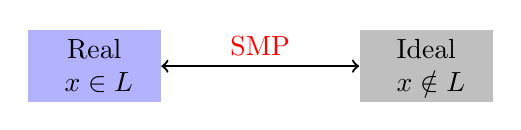
\begin{tikzpicture}
    \node [shapenode, name=real, draw=none, fill=blue!30] {Real \\ ~~~$x \in L$~~~}; 
    
    \node [shapenode, name=ideal, draw=none, right of = real, xshift=12em, fill=gray!50] {Ideal \\ ~~~$x \notin L$~~~}; 

    \draw (real) edge [<->, thick] node [above, red] {SMP} (ideal);
\end{tikzpicture}
\end{center}

\begin{enumerate}
    \item 真实游戏中挑战密文为语言中的随机实例$x \in L$; 
    \item 理想游戏中挑战密文为语言外的随机实例$x \notin L$, 在信息论意义下证明敌手优势可忽略; 
    \item 利用SMP完成语言内外的切换, 论证PPT敌手在真实游戏和理想游戏中的优势差可忽略. 
\end{enumerate}
论证过程与中国道家的``阴阳相生''思想暗合. 

在很多情形下, 公钥加密的私钥嵌入于底层困难问题, 
因此设计高等级安全公钥加密的一个常见难点是归约证明过程中, 归约算法$\mathcal{R}$需要在未知私钥的情形下模拟与私钥相关的谕言机. 
一个具体的例子就是难以证明ElGamal PKE具备私钥抗泄漏安全性, 因为私钥嵌入在底层DDH困难问题中.  
Cramer和Shoup另辟蹊径, 绕过了该难点, 关窍是在基于HPS的公钥加密设计中, 公钥加密的密文嵌入于底层困难问题, 
归约算法$\mathcal{R}$始终掌握私钥, 从而可以完美模拟任意与私钥相关的谕言机. 
正是该特性使得HPS的用途极为广泛, 远远超越了最初的CCA安全的公钥加密, 
如HPS在基于口令的密钥交换(PAKE: Password authenticated key exchange)、
不经意传输(Oblivious transfer)的构造中均有重要应用, 更是达成密钥泄漏安全、消息依赖密钥安全等高等级安全的主流技术工具. 


% \section{More Applications}
% \subsection{Leakage Resilient PKE}
% \begin{frame}{Bounded Leakage Model}
% \begin{trivlist}
%     \item We focus on a simple yet general leakage model called Bounded Leakage Model
% \end{trivlist}

% \begin{center}
% \begin{tikzpicture}
%     \node [name=adv, textnode] {\includegraphics[width=0.5in]{\path/Image/cartoon/adversary.png}};
%     \node [name=challenger, textnode, right of = adv, xshift=15em] 
%         {\includegraphics[width=0.5in]{\path/Image/cartoon/challenger.png}}; 
%     \node [name=Func, right of = challenger, xshift=4em, shapenode, minimum height=3em, thick] {$\mathsf{F}$~~~\red{$sk$}~~~~~}; 

%     \draw ($(adv.east)+(0em, 1em)$) edge[->] node[above] {$g_i$} ($(challenger.west)+(0em, 1em)$);
%     \draw ($(challenger.west)+(0em, -1em)$) edge[->] node[above] {$g_i(sk)$} ($(adv.east)+(0em, -1em)$);

%     \node [name=restriction, below of = adv, xshift=9em, yshift=-4em] 
%         {natural restriction\\$\sum|g_i(\red{sk})| \leq |\red{sk}|$}; 
% \end{tikzpicture}
% \end{center}
% \end{frame}

% \begin{frame}{Leakage-Resilient KEM}
% \begin{definition}[$\ell$-Leakage-Resilience]
% KEM is IND-CPA/CCA $\ell$-leakage-resilient if for any PPT $\mathcal{A}$: 
% \begin{displaymath}
%     \Pr \left[\beta = \beta':
%     \begin{array}{ll}
%         & (pk, sk) \leftarrow \mathsf{Gen}(\lambda);\\
%         & \blue{state \leftarrow \mathcal{A}_1^{\mathcal{O}_\text{leak}(\cdot)}(pk);}\\
%         & (c^*, k^*) \leftarrow \mathsf{Encaps}(pk); \\
%         & k_0^* \leftarrow k^*, k_1^* \sample K;\\
%         & \beta \sample \{0,1\}; \\
%         & \beta' \leftarrow \mathcal{A}_2^{\red{\mathcal{O}_\text{dec}(\cdot)}}(pk, c^*, k_\beta^*);
%     \end{array} 
%     \right] - \frac{1}{2}
% \end{displaymath}
% Here $\mathcal{O}_\text{leak}(\cdot)$ on input $g_i: SK \rightarrow \{0,1\}^*$, outputs $g_i(sk)$. 
% \end{definition}

% \begin{trivlist}
%     \item The only restriction is $\sum|g_i(sk)| \leq \ell$. 
% \end{trivlist}
% \end{frame}

% \begin{frame}{How to achieve provably secure leakage-resilience?}

% \begin{center}
% \begin{tikzpicture}
% \uncover<1->{
%     \node [name=adv, textnode] {\includegraphics[width=0.5in]{\path/Image/cartoon/adversary.png}};
%     \node [name=LRFunc, shapenode, right of = adv, xshift=8em, minimum height=3em, 
%         thick, label={[xshift=0cm, yshift=1em]$\mathcal{R}$}] {$\mathsf{F}$~~\red{$sk$}~~~~};
%     \node [name=assumptions, shapenode, draw=none, rounded corners=1em, minimum height=3em, fill=blue!30, 
%         right of = LRFunc, xshift=8em] {Assumptions}; 
% }

% \uncover<2->{
%     \draw ($(adv.north)+(2em, -0.5em)$) edge[->, thick, bend left] ($(LRFunc.north)+(-1em, 2em)$);
%     \draw ($(LRFunc.north)+(1em, 2em)$) edge[->, thick, bend left] ($(assumptions.west)+(0em, 1.5em)$);
% }

% \uncover<3->{
%     \draw ($(adv.east)+(0em, 0.5em)$) edge[->] node[above] {$g$} ($(LRFunc.west)+(0em, 0.5em)$);
%     \draw ($(LRFunc.west)+(0em, -0.5em)$) edge[->] node[below] {$g(sk)$} ($(adv.east)+(0em, -0.5em)$);
% }
% \uncover<4->{
%     \draw ($(LRFunc.east)+(0em, 0em)$) edge[<->] ($(assumptions.west)+(0em, 0em)$);
%     \draw ($(LRFunc.south)+(0em, 0.7em)$) edge[->, bend right = 60, thick, dashed, color=red] ($(assumptions.south)+(0em, 0em)$);
% }
% \end{tikzpicture}
% \end{center}

% \vspace{-2em}
% \uncover<5->{
% Technical hurdle: a paradox

% \begin{itemize}
%     \item In order to answer \emph{\red{arbitrary}} leakage queries, it seems $\mathcal{R}$ must know $sk$   
%     \item Typically $\mathcal{R}$ does not know $sk$ since the challenge instance is embedded in it 
% \end{itemize}
% }

% \uncover<6->{
% \begin{remarkblock}
%     With HPS, $\mathcal{R}$ always know $sk$ $\leadsto$ $\mathcal{R}$ can handle leakage queries
%     \begin{itemize} 
%         \item hard problem instance is not embedded to $sk$ in HPS
%     \end{itemize}
% \end{remarkblock}
% }
% \end{frame}

% \begin{frame}{Thinking}
% \begin{trivlist}
% \uncover<1->{
%     \item The above KEM based on HPS is CPA-secure, but is insecure against key-leakage attack. 
%         \begin{itemize}
%         \uncover<2->{
%             \item From key leakage, $\mathcal{A}$ gets to learn partial information about $sk$, 
%                 thus $sk$ is not \red{uniformly random} in $\mathcal{A}$'s view anymore.
%         }

%         \uncover<3->{
%             \item Thereby, we can not apply smoothness to argue $\mathsf{H}_{sk}(x^*)$ 
%                 is close to uniform \emph{in the presence of key leakage}. 
%         }  
%         \end{itemize} 
% }

% \vspace{1em}
% \uncover<4->{
% \begin{center}
%     \emph{How to solve this problem?}
% \end{center}
% }
% \end{trivlist}
% \end{frame}


% \begin{frame}{The Seminal Leakage-Resilient PKE in Bounded Leakage Model}
% \uncover<1->{
% \begin{noteblock}
%     \cite{NS-CRYPTO-2009} (CRYPTO 2009): Public-Key Cryptosystems Resilient to Key Leakage
% \end{noteblock}

% \begin{figure}[!hbth]
%     \centering
%     \includegraphics[height=1.2in]{\path/Photo/Moni_Naor.jpeg} \qquad
%     \includegraphics[height=1.2in]{\path/Photo/Gil_Segev.jpg}
%     \caption{Moni Naor \& Gil Segev}
% \end{figure}
% }

% \begin{trivlist}
% \uncover<2->{
%     \item \mdblue{No leakage:} smoothness $\Rightarrow \pi^* \leftarrow \mathsf{H}_{sk}(x^*) \approx_s U_\Pi$, 
%         $sk \sample SK$.  
% }

% \uncover<3->{
%     \item \red{Bounded leakage:} $sk$ is not uniformly random, so does $\pi^*$.  
%         But $\pi^*$ still has sufficient min-entropy
% }
% \end{trivlist}

% \end{frame}


% \begin{frame}{Notions of Entropy}
% \begin{trivlist}
% \uncover<1->{
% \item \mdblue{min-entropy} --- the unpredictability of a random variable $X$: 
%     \begin{equation*}
%         \minentropy(X) = - \log (\max_x \Pr[X = x])
%     \end{equation*}
%     the optimal probability of guessing $X$.  
% }

% \vspace{0.5em}
% \uncover<2->{
% \item \mdblue{average min-entropy} --- the remaining unpredictability of a random variable 
%         $X$ conditioned on another random variable $Y$: 
%     \begin{equation*}
%         \avminentropy(X|Y) = -\log \left(\expect_{y \leftarrow Y} \left[2^{-\minentropy(X|Y = y)}\right]\right)
%     \end{equation*}
%     the optimal probability of guessing $X$, given knowledge of $Y$.  
% }

% \vspace{0.5em}
% \uncover<3->{
% \begin{noteblock}
% \mdblue{Chain Lemma:} If $|Y| = 2^r$, then $\avminentropy(X|Y) \geq \minentropy(X) - r$. 
% \end{noteblock}
% }
% \end{trivlist}
% \end{frame}


% \begin{frame}{Randomness Extractor}
% \begin{definition}[Average-case strong randomness extractor]
% $\mathsf{Ext}: \{0, 1\}^n \times \{0, 1\}^t \rightarrow \{0, 1\}^m$ is an average-case 
% $(\kappa, m)$-strong extractor if for all pairs of random variables $(X,Y)$ such that 
% $X \in \{0,1\}^n$ and $\avminentropy(X|Y) \geq \kappa$ it holds that:
% \begin{equation*}
%     (\mathsf{Ext}(X, S), S, Y) \approx_s (U_m, S, I))
% \end{equation*} 
% where $S$ is uniform over $\{0, 1\}^t$.
% \end{definition} 

% \vspace{1em}

% \begin{remarkblock}
%     Leftover hash lemma states that any family of universal hash functions 
%     is an average-case strong randomness extractor. 
% \end{remarkblock} 
% \end{frame}

% \begin{frame}{Leakage-resilient KEM from HPS}
% \begin{trivlist}
% \item \mdblue{Ingredients:} $(\log |\Pi| - \ell, m)$ average-case strong randomness extractor 
% $\mathsf{Ext}$ (where $\ell$ is the leakage bound), smooth HPS 
% \end{trivlist}
% \begin{construction}[Leakage-resilient KEM from Smooth HPS]
% \begin{itemize}
%     \item $\mathsf{Gen}(\lambda)$: run $(pk, sk) \leftarrow \text{HPS}.\mathsf{Gen}(\lambda)$. 

%     \item $\mathsf{Encaps}(pk;r)$: $C = X$, $K = \{0,1\}^m$ 
%         \begin{enumerate}
%             \item run $(x, w) \leftarrow \mathsf{SampR}(r)$;
%             \item compute $\pi \leftarrow \mathsf{H}_{sk}(x)$ via $\text{HPS}.\mathsf{Pub}(pk, x, w)$;
%             \item pick \redul{$s \sample \{0,1\}^t$};  
%             \item output \redul{$c = (x, s)$}, \redul{$k \leftarrow \mathsf{Ext}(\pi, s)$}. 
%         \end{enumerate}

%     \item $\mathsf{Decaps}(sk, c)$: 
%     \begin{enumerate}
%         \item parse $c = (x, s)$; 
%         \item compute $\pi \leftarrow \text{HPS}.\mathsf{Priv}(sk, x)$; 
%         \item output $k \leftarrow \mathsf{Ext}(\pi, s)$.
%     \end{enumerate} 
% \end{itemize}
% \end{construction} 
% \end{frame}

% \begin{frame}{Security Proof}
% \uncover<1->{
% \begin{noteblock}
% \mdblue{Theorem:} Assuming SMP is hard, the above construction is $\ell$-LR-CPA secure.
% \end{noteblock}
% }
% \uncover<2->{
%     The proof is almost identical to that for plain CPA security. 
% }
% \begin{itemize}
%     \uncover<3->{
%         \item SMP is embedded in the ciphertext, 
%             thus $\mathcal{R}$ always has the real $sk$ to handle all leakage queries. 
%     }

%     \uncover<4->{
%         \item Chain lemma + Smoothness $\Rightarrow$ In the presence of bounded leakage: 
%         \begin{eqnarray*} 
%             \avminentropy(\pi^*|leak) & \geq & \minentropy(\pi^*) - \ell\\
%                                       & = & \log |\Pi| - \ell
%         \end{eqnarray*}
%         \vspace{-1em}
%     }

%     \uncover<5->{
%         \item Apply randomness extractor: 
%         \begin{equation*}
%             k^* \leftarrow \mathsf{Ext}(\pi^*, s^*) \approx_s U_m
%         \end{equation*}
%         \vspace{-1em}
%     }   
% \end{itemize}
% \end{frame}

% \subsection{Lossy Trapdoor Functions}
% \begin{frame}{LTDF from Dual HPS}
% \begin{noteblock}
% \cite{Wee2012-EUROCRYPT} (EUROCRYPT 2012): Dual Projective Hashing and Its Applications
% \end{noteblock}

% \begin{trivlist}
%     \item \mdblue{Key Observation:} $\mathsf{H}_{sk}(x)$ could also be wrote as $\mathsf{H}_x(sk)$
%     \begin{itemize}
%         \item projective $\leadsto$ lossy when $x \in L$
%         \item \red{(informal)} universal $\leadsto$ invertible when $x \notin L$
%     \end{itemize}
% \end{trivlist}

% \begin{definition}[Dual HPS]
% Same as HPS expect universality is replaced by invertibility---
% $\forall (x, \tau) \leftarrow \mathsf{SampNo}(\lambda)$ and $\forall sk$, 
% one can efficiently recover $sk$ from $(\alpha(sk), \mathsf{H}_{x}(sk))$ with $\tau$: 
% \begin{center}
%     $\mathsf{TdInv}(\tau, \alpha(sk), \mathsf{H}_x(sk)) = sk$
% \end{center}
% \end{definition}

% \end{frame}

% \begin{frame}{Connection Between LTDF and HPS}
% \begin{construction}[LTDF from Dual HPS]
% \begin{itemize}
%     \item $\mathsf{Gen}(\lambda; inj)$: run $(x, \tau) \leftarrow \mathsf{SampNo}(\lambda)$, output $x$ and $\tau$
%     \item $\mathsf{Gen}(\lambda; lossy)$: run $(x, w) \leftarrow \mathsf{SampYes}(\lambda)$, output $x$ and $\bot$
%     \item $\mathsf{Eval}(x, sk)$: \redul{treat $x$ as evaluation key and $sk$ as input}
%     \begin{center}
%         $F_x(sk): = \alpha(sk)||\mathsf{H}_x(sk)$
%     \end{center}

%     \item $\mathsf{Invert}(\tau, y_0||y_1)$: output $\mathsf{TdInv}(\tau, y_0||y_1)$
% \end{itemize}
% \end{construction}

% \begin{noteblock}
%     \mdblue{Theorem:} Under the SMP, the above construction yields a collection of $(n, \log|\text{Img}(\alpha)|)$-LTDF.
% \end{noteblock}

% \begin{itemize}
%     \item Correctness for injective mode $\Leftarrow$ Invertibility
%     \item Lossiness for lossy mode: $\text{Img}(F_x) = \text{Img}(\alpha)$ for $x \in L$ $\Leftarrow$ Projective property
%     \item Injective $\approx_c$ Lossy $\Leftarrow$ SMP
% \end{itemize}
% \end{frame}

% \begin{frame}{More Thinking}
% \begin{trivlist}
% \item \red{Shortcomings} of \redul{Dual HPS $\Rightarrow$ LTDF}
% \begin{itemize}
%     \item require HPS satisfying invertibility $\leadsto$ reduce generality
%     \item no efficient ABO construction is known 
% \end{itemize}

% \vspace{1em}
% \item \mdblue{Observation:} 
% \begin{itemize}
%     \item invertibility or even injectivity is not necessary for some applications
%     \item efficient ABO construction is possible by exploiting algebra structure of SMP
% \end{itemize}
% \end{trivlist}
% \end{frame}

% \begin{frame}{(Algebra) Subset Membership Problem}
% \uncover<1->{
% \begin{center}
% \begin{tikzpicture}
%     \draw (0, 2) node {$U_X \approx_c U_L$};
%     \draw [color=gray!40, fill=gray!40] (0,0) circle (1cm);
%     \draw (0,0.7) node {$X$};
%     \draw [color=violet!70, fill=violet!70] (0,0) circle (0.4cm);
%     \draw (0,0) node {$L$};
%     \draw [color=cyan, fill=cyan] (4,0) circle (0.4cm);
%     \draw (4,0) node {$W$}; 
%     \draw [<->, thin] (0.4,0) -- (3.6,0);
%     \draw (2,0.2) node {$\mathsf{R}_L$};
%     \draw [color=black] (2, -1) node {$\mathsf{SampR}(\lambda)$}; 
%     \draw [color=black] [->, thin] (1.8, -0.8) -- (0.3, -0.3);
%     \draw [color=black] [->, thin] (2.2, -0.8) -- (3.7, -0.3);

%     \draw [color=black] (-3, 1) node {$\mathsf{SampAll}(\lambda)$};
%     \draw [color=black] (-3, 0) node {$\mathsf{SampYes}(\lambda)$};
%     \draw [color=black] (-3, -1) node {$\mathsf{SampNo}(\lambda)$}; 

%     \draw [color=black] [->, thin] (-2,1) -- (-0.72,0.65);
%     \draw [color=black] [->, thin] (-2,0) -- (-0.4,0);
%     \draw [color=black] [->, thin] (-2,-1) -- (-0.5,-0.5); 
% \end{tikzpicture}
% \end{center}
% }

% \uncover<2->{
% Algebra SMP (mild \& natural)
%     \begin{itemize}
%         \item $X$ forms an Abelian group, $L$ forms a subgroup of $X$
%         \item Quotient group $H = X/L$ is cyclic and $\#(H) = |X|/|L| = p$
%     \end{itemize}    
% }

% \uncover<3->{
% Algebraic properties $\leadsto$ two useful facts
% \begin{enumerate}
%     \item Let $\bar{a} = aL$ for some $a \in X \backslash L$ be a generator of $H$, 
%         the co-sets $(aL, 2aL, \dots, (p-1)aL, paL = L)$ constitute a partition of $X$. 

%     \item For each $x \in L$, $ia+x \notin L$ for $1 \leq i <p$
% \end{enumerate}
% }

% \end{frame}

% \begin{frame}{ABO-RLF from HPS for ASMP}
% \uncover<1->{
% Let $aL$ be a generator for $H = X/L$, we build ABO-RLF from HPS for ASMP as below: 
% \begin{itemize}
%     \item $\mathsf{Gen}(\lambda, b^*)$: $(x, w) \leftarrow \mathsf{SampYes}(\lambda)$, 
%         output $ek = -b^*a + x$
%     \item $f_{ek,b}(sk)$: output $\alpha(sk)||\mathsf{H}_{sk}(ek+ba)$
% \end{itemize}
% }

% \uncover<2->{
% \begin{noteblock}
% \mdblue{\textbf{Lemma:}} Assume $g_x(sk):=\alpha(sk)||\mathsf{H}_{sk}(x)$ is $v$-regular for any $x \notin L$. 
% The above construction is $(v, \log |\textup{Img} \alpha|)$-ABO-RLF under ASMP. 
% \end{noteblock}
% }

% \uncover<3->{
% \begin{itemize}
%     \item $ek+ba = x + (b-b^*)a \notin L$ if $b \neq b^*$ $\Rightarrow$ $v$-regular
%     \item $ek+ba = x + (b-b^*)a \in L$ if $b = b^*$ $\Rightarrow$ lossy by the projective property
%     \item ASMP $\Rightarrow$ Hidden lossy branch. For any $b_0^*, b_1^* \in \mathbb{Z}_p$: 
%     \begin{equation*}
%         (-b_0^*a+x) \approx_c (-b_0^*a+u) \equiv (-b_1^*a+u) \approx_c (-b_1^*a+x)
%     \end{equation*}
%     where $u \sample X$. 
% \end{itemize}
% }

% \end{frame}

% \subsection{Lossy Encryption}
% \begin{frame}{Lossy Encryption}
% \begin{trivlist}
% \item Peikert, Vaikuntanathan, Waters: Dual Mode Encryption
% \begin{noteblock}
% \cite{PVW2008} (CRYPTO 2008): A Framework for Efficient and Composable Oblivious Transfer
% \end{noteblock}

% \item Bellare, Hofheinz, Yilek: Lossy Encryption
% \begin{noteblock}
% \cite{BHY2009} (EUROCRYPT 2009): Possibility and impossibility results for encryption and commitment 
%     secure under selective opening
% \end{noteblock}

% \begin{itemize}
%     \item injective public keys: normal encryption
%     \item lossy public keys: lossy encryption --- encryptions of any two plaintexts under a lossy key 
%         yield distributions that are statistically close
%     \item injective public keys $\approx_c$ lossy public keys
% \end{itemize}

% \end{trivlist}
% \end{frame}

% \begin{frame}{Lossy KEM}
% \begin{trivlist}
% \item We can define lossy KEM analogously to lossy encryption
% \begin{itemize}
%     \item injective public keys: normal encapsulation
%     \item lossy public keys: lossy encapsulation --- encapsulated key is statistically close to uniform 
%     \item injective public keys $\approx_c$ lossy public keys
% \end{itemize}
% \end{trivlist}

% \begin{center}
%     Lossy Encryption $\Leftrightarrow$ Lossy KEM 
% \end{center}
% \end{frame}

% \begin{frame}{Lossy KEM from HPS}
% \begin{trivlist}
%     \item \mdblue{Main idea:} dual use of HPS
% \end{trivlist}


% \centering
% \begin{tabular}{|c|c|c|c|c|}

% \hline
%            & $pk$       & $sk$         & $x$        & $w$\\
% \hline
% normal use & public key & secret key   & ciphertext & randomness\\
% \hline
% dual use   & ciphertext & randomness & public key & secret key\\
% \hline
% \end{tabular}

% \begin{construction}[Lossy KEM from smooth HPS]
% \begin{itemize}
%     \item $\mathsf{Gen}(\lambda, inj)$: $(x, w) \leftarrow \mathsf{SampYes}(\lambda)$, 
%         output $x$ as public key and $w$ as secret key. 

%     \item $\mathsf{Gen}(\lambda, lossy)$: $x \leftarrow \mathsf{SampNo}(\lambda)$, output $x$ as public key. 

%     \item $\mathsf{Encaps}(x; r)$: $(pk, sk) \leftarrow \text{HPS}.\mathsf{Gen}(\lambda; r)$, 
%         output $pk$ as ciphertext and compute $\mathsf{H}_{sk}(x)$ via $\text{HPS}.\mathsf{Priv}(sk, x)$ 
%         as encapsulated key. 

%     \item $\mathsf{Decaps}(w, c)$: recover $\mathsf{H}_{sk}(x)$ via $\text{HPS}.\mathsf{Pub}(c, x, w)$.  
% \end{itemize}
% \end{construction}
% \end{frame}


\section{可提取哈希证明系统类}
\begin{center}
    事要知其所以然.  \\
                \hfill --- 《朱子语类·卷九·论行知》
\end{center}


1991年, Rackoff和Simon~\cite{RS-CRYPTO-1991}提出了构造CCA安全PKE的另一条技术路线: 
\begin{enumerate}
	\item 发送方随机选择会话密钥$k$并使用接收方的公钥对其加密得到密文$c$, 同时生成关于$k$的非交互零知识知识证明$\pi$, 将$c$和$\pi$一起发送给接收方;  
	\item 接收方先验证$\pi$的正确性, 若验证通过则利用私钥解密恢复会话密钥; 
\end{enumerate}
该条技术路线被称为Rackoff-Simon范式, 与Naor-Yung范式/Sahai范式的不同之处是前者需要使用非交互零知识知识的证明(NIZKPoK), 而后者使用的势非交互零知识证明(NIZK). 

Cramer和Shoup于2002年正式提出的哈希证明系统是NIZK的弱化: 公开可验证弱化为指定验证者, 表达能力由任意$\mathcal{NP}$语言限制为群论语言, 证明的形式特化为哈希值. 
2010年, Wee~\cite{Wee-CRYPTO-2010}提出了可提取哈希证明系统(EHPS, extractable hash proof system), 
并展示了如何基于EHPS以一种简洁、模块化的方式构造CCA安全的PKE. 该构造范式统一了几乎所有已知的基于计算性假设的CCA安全PKE方案.  
相对HPS是NIZK的弱化, EHPS是NIZKPoK的弱化. 以下首先介绍EHPS的定义和相关性质. 

\begin{definition}[可提取哈希证明系统]
EHPS包含以下多项式时间算法:
\begin{itemize}
\item $\mathsf{Setup}(1^\kappa)$: 以安全参数$\kappa$为输入, 输出公开参数$pp = (\mathsf{H}, PK, SK, L, W, \Pi)$, 
	其中$L$是由困难关系$\mathsf{R}_L$定义的平凡$\mathcal{NP}$语言, 
	$\mathsf{H}: PK \times L \rightarrow \Pi$是由公钥集合$PK$索引的一族带密钥哈希函数. 
	关系$\mathsf{R}_L$支持随机采样, 即存在PPT算法$\mathsf{SampRel}$以随机数$r$为输入, 输出随机的``实例-证据''元组$(x, w) \in \mathsf{R}_L$.  
	为了方便后续的应用, $\mathsf{SampRel}$可以进一步分解为$\mathsf{SampIns}$和$\mathsf{SampWit}$, 前者随机采样语言中的实例, 后者随机采样证据, 
	对于任意随机数$r \in R$, 我们有$(\mathsf{SampIns}(r), \mathsf{SampWit}(r)) \in \mathsf{R}_L$. 

\item $\mathsf{KeyGen}(pp)$: 以公开参数$pp$为输入, 输出公钥$pk$和私钥$sk$. 

\item $\mathsf{PubEval}(pk, x, r)$: 以公钥$pk$、$x \in L$和随机数$r$为输入, 输出证明$\pi \in \Pi$. 
	正确性要求是当$r$是采样$x$的随机数时(即$(x, w) \leftarrow \mathsf{SampRel}(r)$), 算法正确计算出哈希证明: $\pi = \mathsf{H}_{pk}(x)$. 
	注意, 当给定采样随机数$r$时, 可以运行算法$\mathsf{SampRel}$恢复$x$, 因此算法的第2项输入$x$可以省去.   

\item $\mathsf{Ext}(sk, x, \pi)$: 以私钥$sk$, $x \in L$和证明$\pi \in \Pi$为输入, 输出证据$w \in W \cup \bot$. 
	正确性要求是: 
	\begin{equation*}
		\pi = \mathsf{H}_{pk}(x) \iff (x, \mathsf{Ext}(sk, x, \pi)) \in \mathsf{R}_L
	\end{equation*}

\item $\mathsf{KeyGen}'(pp)$: 以公开参数$pp$为输入, 输出公钥$pk$和私钥$sk'$. 

\item $\mathsf{PrivEval}(sk', x)$: 以私钥$sk$和$x \in L$为输入, 输出证明$\pi \in \Pi$. 
	正确性要求是$\mathsf{PrivEval}$正确计算出哈希证明: $\pi = \mathsf{H}_{pk}(x)$. 
\end{itemize}
以上算法中, $\mathsf{KeyGen}$、$\mathsf{PubEval}$和$\mathsf{Ext}$工作在真实模式, 
$\mathsf{KeyGen}'$和$\mathsf{PrivEval}$工作在模拟模式, 两种模式共享同一个$\mathsf{Setup}$算法生成公开参数. 
两种模式之间的关联是公钥的分布统计不可区分, 即: 
\begin{equation*}
	\mathsf{KeyGen}(pp)[1] \approx_s \mathsf{KeyGen}'(pp)[1]
\end{equation*}
\end{definition}

\begin{figure}[!hbtp]
\begin{center}
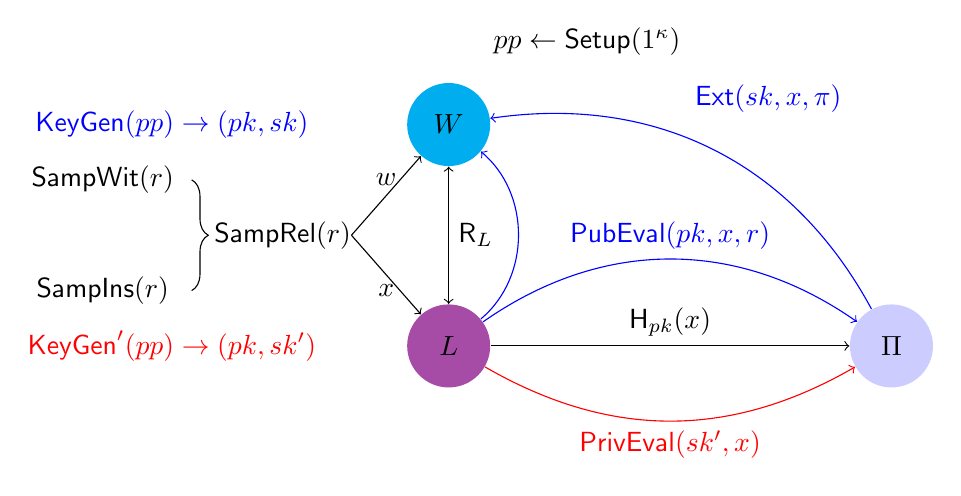
\begin{tikzpicture}
	\node [textnode, name=setup] {$pp \leftarrow \mathsf{Setup}(1^\kappa)$}; 	

    \node [circlenode, name = W, draw = none, fill=cyan, minimum size=3em, below of = setup, xshift=-5em, yshift=-3em] {$W$}; 
    \node [circlenode, name = L, below of = W, draw=none, fill=violet!70, minimum size=3em, yshift=-8em] {$L$}; 
    \node [circlenode, name = Pi, right of = L, draw=none, fill=blue!20, minimum size=3em, xshift=16em] {$\Pi$}; 

    \node [textnode, name=sample, below of = W, xshift=-6em, yshift=-4em] {$\mathsf{SampRel}(r)$}; 

    \draw[decorate, decoration={brace,raise=2pt, amplitude=6pt}, thin]
    ($(sample.west)+(-1em, 2em)$)--($(sample.west)+(-1em, -2em)$); 

    \node [textnode, name=SampWit, left of = sample, xshift=-6.5em, yshift=2em] {$\mathsf{SampWit}(r)$}; 
    \node [textnode, name=SampIns, left of = sample, xshift=-6.5em, yshift=-2em] {$\mathsf{SampIns}(r)$}; 

    \draw (sample.east) edge[->] node[above] {$w$} (W); 
    \draw (sample.east) edge[->] node[below] {$x$} (L);

    \node [textnode, name=Gen, left of = W, xshift=-10em, color=blue] {$\mathsf{KeyGen}(pp) \rightarrow (pk, sk)$}; 
    \node [textnode, name=Genprime, left of = L, xshift=-10em, color=red] {$\mathsf{KeyGen}'(pp) \rightarrow (pk, sk')$}; 


    \draw (W) edge[<->] node[right] {$\mathsf{R}_L$} (L); 
    \draw (L) edge[->] node[above] {$\mathsf{H}_{pk}(x)$} (Pi); 
    \draw (L) edge[->, bend left=35, color=blue] node[above] {\blue{$\mathsf{PubEval}(pk, x, r)$}} (Pi); 
    \draw (Pi) edge[->, bend right=35, color=blue] 
        node[above, xshift=2em, yshift=1em] {\blue{$\mathsf{Ext}(sk, x, \pi)$}} (W); 

    \draw (L) edge[->, bend right=50, color=blue] (W); 
    \draw (L) edge[->, bend right=30, color=red] node[below] {\red{$\mathsf{PrivEval}(sk', x)$}} (Pi); 
\end{tikzpicture}
\end{center}
\caption{EHPS的示意图}
\end{figure}


\subsection{起源释疑}

\begin{figure}[!hbtp]
\begin{center}
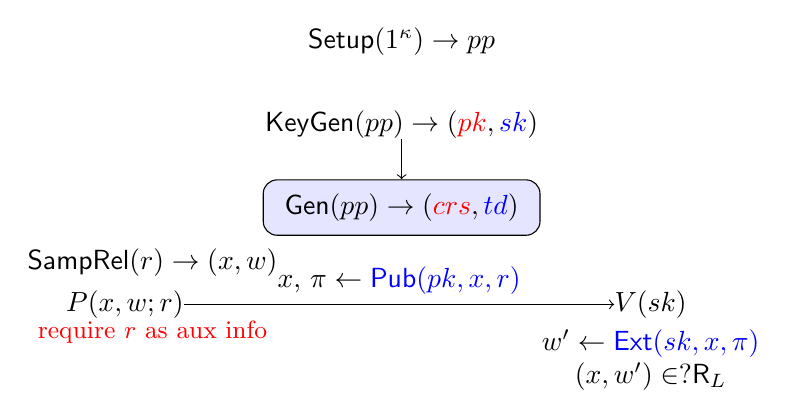
\begin{tikzpicture}
	\node [textnode, name=Setup] {$\mathsf{Setup}(1^\kappa) \rightarrow pp$}; 
    \node [textnode, name=KeyGen, below of = Setup, yshift=-3em] {$\mathsf{KeyGen}(pp) \rightarrow (\red{pk}, \blue{sk})$};
    \node [roundnode, fill=blue!10, name=ZKGen, below of=KeyGen, yshift=-3em, minimum width=10em, minimum height=2em] 
    	{$\mathsf{Gen}(pp) \rightarrow (\red{crs}, \blue{td})$};
    \draw (KeyGen) edge[->] (ZKGen);

	\node [textnode, name=SampR, below of=ZKGen, xshift=-9em, yshift=-2em] {$\mathsf{SampRel}(r) \rightarrow (x, w)$};
	\node [textnode, name=Prover, below of=ZKGen, xshift=-10em, yshift=-3.5em] {$P(x, w; r)$};
	\node [textnode, below of=ZKGen, xshift=-9em, yshift=-4.5em, color=red, font=\small] 
    	{require $r$ as aux info};
	\node [textnode, name=Verifier, below of=ZKGen, xshift=9em, yshift=-3.5em] {$V(sk)$};  
	\node [textnode, name=check, below of=Verifier, yshift=-2em] {
		$w' \leftarrow \blue{\mathsf{Ext}(sk, x, \pi)}$ \\ $(x, w') \in ? \mathsf{R}_L$};
	\draw (Prover) edge[->] node[above] {$x$, $\pi \leftarrow \blue{\mathsf{Pub}(pk, x, r)}$} (Verifier);
\end{tikzpicture}
\end{center}
\caption{从DV-NIZKPoK的视角解析EHPS}
\end{figure}

\begin{note}
上图解释了EHPS的命名渊源, 其本质上是指定验证者零知识知识的证明, 证明的形式是实例的哈希值, 故名可提取哈希证明系统. 
\begin{itemize}
\item DV-NIZKPoK的完备性和可提取性由$\mathsf{Ext}$的正确性保证, 即在正常模式下,  
	\begin{equation*}
    	\pi = \mathsf{H}_{pk}(x) \iff (x, \blue{\mathsf{Ext}(sk, x, \pi)}) \in \mathsf{R}_L
	\end{equation*} 
其中$\mathsf{KeyGen}(pp) \rightarrow (pk, sk)$.

\item DV-NIZKPoK的零知识性论证如下, 令$\mathsf{KeyGen}(pp) \rightarrow (\blue{pk}, sk')$, 
	$\mathsf{KeyGen}'(pp) \rightarrow (\red{pk}, sk')$, 对于$\forall x \in L$, 我们有: 
	\begin{equation*}
		\blue{pk} \approx_s \red{pk} \Rightarrow (\blue{pk}, \mathsf{H}_{\blue{pk}}(x)) \approx_s (\red{pk}, \mathsf{H}_{\red{pk}}(x))
	\end{equation*} 
	再由秘密求值算法的正确性$\mathsf{H}_{\red{pk}}(x) = \mathsf{PrivEval}(sk', x)$可以得到:  
	\begin{equation*}
		(\blue{pk}, \mathsf{H}_{\blue{pk}}(x)) \approx_s (\red{pk}, \mathsf{PrivEval}(sk', x))
	\end{equation*} 
\end{itemize}
\end{note}

\subsection{EHPS的构造}
我们以针对$L_\text{CDH}$语言的EHPS构造为例, 获得对EHPS设计方式的直观认识. 
令$(\mathbb{G}, p, g)$是算法$\mathsf{GroupGen}(1^\kappa)$的输出, 其中$\mathbb{G}$是阶位素数$p$的群, 
$g$是生成元. 随机选取$\mathbb{G}$中的另一生成元$g^\alpha$, 其中$\alpha \sample \mathbb{Z}_p$. 
令$pp = (\mathbb{G}, p, g, g^\alpha)$是公开参数, 定义由$pp$索引的平凡$\mathcal{NP}$语言如下:  
\begin{equation*}
	L_\text{CDH} = \{x \in X: \exists w \in W \text{~s.t.~} w = x^\alpha\}
\end{equation*}
其中$L = X = \mathbb{G}$, $W = \mathbb{G}$. 
定义$L_\text{CDH}$的二元关系为$\mathsf{R}_\text{CDH}$,	$(x, w) \in \mathsf{R}_\text{CDH} \iff w = x^\alpha$. 
容易验证: 
\begin{itemize}
	\item $\mathsf{R}_\text{CDH}$基于CDH假设是困难的. 
	
	\item $\mathsf{R}_\text{CDH}$是高效可采样的: 存在PPT采样算法$\mathsf{SampRel}$随机选取$r \sample \mathbb{Z}_p$, 
		输出 $(g^r, (g^{\alpha})^r) \in \mathsf{R}_\text{CDH}$. 

    \item 如果$\mathbb{G}$是双线性映射群, 则$\mathsf{R}_\text{CDH}$是公开可验证的.  
\end{itemize}

\begin{construction}[$L_\text{CDH}$语言的EHPS构造]
$L_\text{CDH}$的EHPS构造如下, 如图所示: 
\begin{itemize}
\item $\mathsf{Setup}(1^\kappa)$: 以安全参数$\kappa$为输入, 输出公开参数$pp = (\mathbb{G}, p, g, g^\alpha)$. 
	其中$pp$还包括了对$SK = \mathbb{Z}_p$, $PK = \mathbb{G}$, $L_\text{CDH} = X = \mathbb{G}$和$W = \mathbb{G}$的描述. 

\item $\mathsf{KeyGen}(pp)$: 以公开参数$pp$为输入, 随机采样$sk \sample \mathbb{Z}_p$, 
	计算$pk = g^{sk} \in \mathbb{G}$, 输出$(pk, sk)$. 

\item $\mathsf{PubEval}(pk, x, r)$: 以公钥$pk$、实例$x \in L_\text{CDH}$和$r \in \mathbb{Z}_p$为输入, 输出$\pi \leftarrow (g^{\alpha} \cdot pk)^r$. 

\item $\mathsf{Ext}(sk, x, \pi)$: 以私钥$sk$、实例$x \in L_\text{CDH}$和$\pi$为输入, 计算$w \leftarrow \pi /x^{sk}$, 
	如果$(x, w) \in \mathsf{R}_L$则返回$w$, 否则返回$\bot$. 正确性由以下公式保证: 
	\begin{equation*}
		\pi /x^{sk} = (g^{\alpha} \cdot pk)^r /x^{sk} = (g^{\alpha} \cdot g^{sk})^r /g^{r \cdot sk} = (g^\alpha)^r = w 
	\end{equation*}

\item $\mathsf{KeyGen}'(pp)$: 以公开参数$pp$为输入, 随机采样$sk' \sample \mathbb{Z}_p$, 计算$pk \leftarrow g^{sk'}/g^\alpha$. 

\item $\mathsf{PrivEval}(sk', x)$: 以私钥$sk'$和实例$x \in L_\text{CDH}$为输入, 输出$w \leftarrow x^{sk'}$.  正确性由以下公式保证: 
	\begin{equation*}
		\mathsf{H}_{pk}(x) = (g^\alpha \cdot pk)^r = (g^{\alpha} \cdot \underline{g^{sk'}/g^\alpha})^r = (g^{sk'})^r = x^{sk'}
	\end{equation*}	
\end{itemize}

容易验证, 两种模式下生成的$pk$服从同样的分布—$\mathbb{G}$上的均匀分布. 
\end{construction}

\begin{figure}[!hbtp]
\begin{center}
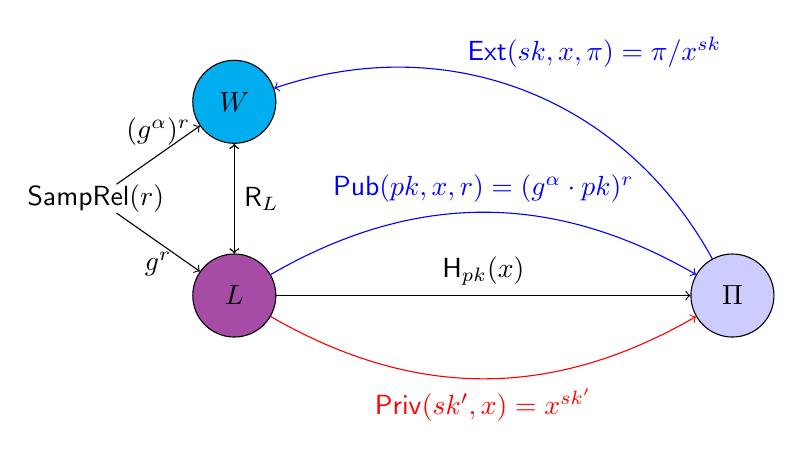
\begin{tikzpicture}
    \node [textnode, name=sample] {$\mathsf{SampRel}(r)$};
    \node [circlenode, name=W, right of = sample, xshift=5em, yshift=3.5em, fill=cyan, minimum size=3em] {$W$}; 
    \node [circlenode, name=L, right of = sample, xshift=5em, yshift=-3.5em, fill=violet!70, minimum size=3em] {$L$}; 
    \node [circlenode, name=Pi, right of = L, xshift=18em, fill=blue!20, minimum size=3em] {$\Pi$}; 

    \draw (L) edge[<->] (W); 
    \draw (L) edge[->] node[above] {$\mathsf{H}_{pk}(x)$} (Pi); 
    \draw (L) edge[->, color=blue, bend left=30] node[above] {$\mathsf{Pub}(pk, x, r) = (g^\alpha \cdot pk)^r$} (Pi); 
    \draw (Pi) edge[->, color=blue, bend right=40] node[above, xshift=2.5em, yshift=0.5em] {$\mathsf{Ext}(sk, x, \pi) = \pi/x^{sk}$} (W); 
    \draw (L) edge[->, color=red, bend right=30] node[below] {$\mathsf{Priv}(sk', x) = x^{sk'}$} (Pi); 
    
    \draw (sample) edge[->] node[above] {$(g^\alpha)^r$} (W); 
    \draw (sample) edge[->] node[below] {$g^r$} (L); 

    \draw (W) edge[<->] node[right] {$\mathsf{R}_L$} (L); 
\end{tikzpicture}
\end{center}
\caption{$L_\text{CDH}$的EHPS}
\end{figure}


\subsection{基于EHPS构造IND-CPA KEM}
作为暖场应用, 我们首先介绍如何基于EHPS构造CPA安全的KEM. 设计的思路源自Rackoff-Simon范式.
令$\mathsf{R}_L$为定义在$X \times W$上的单向关系, $\mathsf{hc}: W \rightarrow K$为相应的hardcore function. 
\begin{itemize}
\item 发送方扮演EHPS中的证明者, 运行$\mathsf{SampRel}(r)$算法随机采样$(x, w) \in \mathsf{R}_L$, 
    利用公钥$pk$和随机数$r$计算$x$的哈希证明$\pi$, 生成密文$c = (x, \pi)$, 计算证据$w$的hardcore function值作为会话密钥$k$. 

\item 接收方扮演EHPS中的验证者: 使用私钥$sk$从密文$(x, \pi)$中恢复$w$, 进而恢复会话密钥.
\end{itemize}

\begin{construction}[基于EHPS的CPA安全KEM]\label{construction:CPA-KEM-from-EHPS}
从语言$L$的EHPS出发, 构造CPA安全的KEM如下:
\begin{itemize}
\item $\mathsf{Setup}(1^\kappa)$: 运行$pp \leftarrow \text{EHPS}.\mathsf{Setup}(1^\kappa)$, 
	输出$pp = (\mathsf{H}, SK, PK, X, L, W, \Pi)$作为公开参数, 
	其中$X \times \Pi$作为密文空间, $\mathsf{R}_L$hardcore function的值域$K$作为会话密钥空间.   

\item $\mathsf{KeyGen}(pp)$: 运行$(pk, sk) \leftarrow \text{EHPS}.\mathsf{KeyGen}(\lambda)$, 输出公钥$pk$和私钥$sk$. 

\item $\mathsf{Encaps}(pk;r)$: 以公钥$pk$和随机数$r$为输入, 执行如下步骤: 
\begin{enumerate}
	\item 运行$(x, w) \leftarrow \mathsf{SampRel}(r)$生成随机实例和相应证据;
     
    \item 通过$\text{EHPS}.\mathsf{Pub}(pk, x, r)$计算实例$x$的哈希证明$\pi \leftarrow \mathsf{H}_{pk}(x)$;  
    
    \item 输出$(x, \pi)$作为密文, 计算$k \leftarrow \mathsf{hc}(w)$作为会话密钥. 
\end{enumerate}

\item $\mathsf{Decaps}(sk, c)$: 以私钥$sk$和密文$c = (x, \pi)$为输入, 
	计算$w \leftarrow \text{EHPS}.\mathsf{Ext}(sk, x, \pi)$, 
    如果$(x, w) \notin \mathsf{R}_L$则输出$\bot$, 否则输出$k \leftarrow \mathsf{hc}(w)$. 
\end{itemize}
\end{construction} 

KEM的正确性由EHPS的完备性和$\mathsf{R}_L$的单射性保证, 安全性由如下定理保证. 

\begin{theorem}
如果$\mathsf{R}_L$是单向的, 那么构造~\ref{construction:CPA-KEM-from-EHPS}中的KEM是IND-CPA安全的. 
\end{theorem}

\begin{proof}
证明的目标是论证会话密钥$\mathsf{hc}(w^*)$在敌手$\mathcal{A}$的视图中是伪随机的, 其中$\mathcal{A}$的视图包括: 

\begin{itemize}
	\item 公开参数$pp$; 
	\item 公钥$pk$: 与$w^*$无关; 
    \item 密文$c^* = (x^*, \pi^*)$: $\mathsf{R}_L$的单向性保证了$x^*$隐藏了$w^*$, 
    	EHPS的零知识性进一步保证了$\pi^*$(相对于$x^*$)不会额外泄漏关于$w^*$的信息. 
\end{itemize}

我们通过以下的游戏序列组织证明.
\begin{trivlist}
\item $\text{Game}_0$: 对应真实的游戏. $\mathcal{CH}$在真实模式下运行EHPS与敌手$\mathcal{A}$交互.
\begin{itemize}
\item 初始化: $\mathcal{CH}$计算$pp \leftarrow \text{EHPS}.\mathsf{Setup}(1^\kappa)$, 
	\redul{$(pk, sk) \leftarrow \text{EHPS}.\mathsf{KeyGen}(pp)$}, 将$pp$和$pk$发送给$\mathcal{A}$. 
        
\item 挑战: $\mathcal{CH}$按照以下步骤生成挑战 
\begin{enumerate}
    \item 随机采样$(x^*, w^*) \leftarrow \mathsf{SampRel}(r^*)$;  
    \item 通过\redul{$\text{EHPS}.\mathsf{PubEval}(pk, x^*, r^*)$}公开计算$\pi^* \leftarrow \mathsf{H}_{pk}(x^*)$; 
    \item 计算$k_0^* \leftarrow \mathsf{hc}(w^*)$, 随机采样$k_1^* \sample K$; 
    \item 随机选取$\beta \sample \{0,1\}$, 将$(c^* = (x^*, \pi^*), k_\beta^*)$发送给$\mathcal{A}$作为挑战. 
\end{enumerate}

\item 应答: $\mathcal{A}$输出对$\beta$的猜测$\beta'$, $\mathcal{A}$成功当且仅当$\beta' = \beta$. 
\end{itemize}

为了利用EHPS的零知识性论证$\pi^*$不额外泄漏关于$w^*$的信息, 需要将EHPS由真实模式切换到模拟模式. 
\item $\text{Game}_1$: $\mathcal{CH}$在模拟模式下运行EHPS与敌手$\mathcal{A}$交互. 
\begin{itemize}
\item 初始化: $\mathcal{CH}$计算\redul{$(pk, sk') \leftarrow \text{EHPS}.\mathsf{KeyGen}'(pp)$}. 
\item 挑战: $\mathcal{CH}$在第二步通过\redul{$\text{EHPS}.\mathsf{Priv}(sk', x^*)$}计算$\pi^* \leftarrow \mathsf{H}_{pk}(x^*)$.
\end{itemize}
\end{trivlist}
敌手$\mathcal{A}$在游戏中的视图为$(pp, pk, x^*, k_\beta^*)$. 容易验证, EHPS的零知识性保证了$\text{Game}_0 \approx_s \text{Game}_1$: 


\begin{claim}
如果$\mathsf{R}_L$是单向的, $\AdvA^{\text{Game}_1} = \mathsf{negl}(\kappa)$. 
\end{claim}

\begin{proof}
证明思路是如果存在$\mathcal{A}$以不可忽略的优势赢得$\text{Game}_1$, 那么可以构造出$\mathcal{B}$以不可忽略的优势打破$\mathsf{hc}$的伪随机性, 从而与单向性假设冲突. 
给定关于$\mathsf{hc}$的伪随机性挑战$pp$和$(x^*, k_\beta^*)$, 其中$(x^*, w^*) \leftarrow \mathsf{SampRel}(r^*)$, 
$\mathcal{B}$模拟$\text{Game}_1$中的挑战者$\mathcal{CH}$与$\mathcal{A}$交互, 目标是猜测$\beta$. 
\begin{itemize}
\item $\mathcal{B}$运行EHPS的模拟模式与$\mathcal{A}$在$\text{Game}_1$进行交互, 
	在初始化阶段不再采样$x^*$而是直接嵌入接收到的$x^*$, 在挑战阶段将$\mathsf{R}_L$的挑战$(x^*, k_\beta^*)$作为$\mathcal{A}$的KEM挑战. 
    最终, $\mathcal{B}$输出$\mathcal{A}$的猜测$\beta'$. 
\end{itemize} 
容易验证, $\mathcal{B}$在$\text{Game}_1$中的模拟是完美的. 因此$\mathcal{B}$打破$\mathsf{R}_L$伪随机性的优势与$\AdvA^{\text{Game}_1}$相同.  
断言得证! \qed
\end{proof}

综上, 定理得证! \qed
\end{proof}


\subsection{基于EHPS构造IND-CCA KEM}
我们首先从安全归约的角度分析基于EHPS构造IND-CCA KEM的难点. 
EHPS模拟模式下的$sk'$可以在不知晓采样实例$x$随机数的情况下正确计算出相应的哈希证明, 但无法提取出证据, 因此归约算法无法应答解密询问.  
因此, 为了构造IND-CCA的KEM, 需要赋予EHPS更丰富的功能. 

PKE/KEM的选择密文安全游戏是``全除一''(ABO, all-but-one)式的—$\mathcal{A}$可以发起除挑战密文$x^*$以外的任意解密/解封装询问. 
Wee~\cite{Wee-CRYPTO-2010}引入了量身定制的ABO-EHPS. 

\begin{definition}{ABO-EHPS}
ABO-EHPS与EHPS的定义差别集中在模拟模式, 真实模式下完全相同. 与EHPS相比, ABO-EHPS在模拟模式下的功能更加丰富.  
\begin{itemize}
    \item $\mathsf{KeyGen}'(pp, x^*)$: 以公开参数$pp$和$x^* \in L$为输入, 输出$(pk, sk')$. 

    \item $\mathsf{PrivEval}(sk', x^*)$: 以私钥$sk'$和$x^*$为输出, 输出证明$\pi^* = \mathsf{H}_{pk}(x^*)$. 

    \item $\mathsf{Ext}'(sk', x, \pi)$: 以私钥$sk'$、$x \neq x^*$和$\pi \in \Pi$为输入, 输出证据$w \in W$. 
    	正确性的要求是:  
    \begin{equation*}
        \pi  = \mathsf{H}_{pk}(x) \iff (x, \mathsf{Ext}'(sk', x, \pi)) \in \mathsf{R}_L
    \end{equation*}
\end{itemize}

$\mathsf{KeyGen}'$算法以预先嵌入的点$x^*$为输入, 输出相应的密钥对$(pk, sk')$. 
ABO的含义是模拟模式中的$sk'$具备以下功能: 
\begin{itemize}
    \item ``一除全''哈希求值(one-out-all evaluation): $sk'$可以计算$x^*$的哈希值$\mathsf{H}_{pk}(x^*)$. 
    \item ``全除一''证据抽取(all-but-one extraction): $sk'$可以从除$x^*$以外的点$x$和相应的证明中正确抽取出证据$\mathsf{Ext}'(sk', x, \pi)$.  
\end{itemize}
\end{definition}

\begin{remark}
模拟模式下$sk'$的功能在CCA安全归约中起到如下作用: 
\begin{itemize}
	\item ``一除全''哈希求值允许归约算法$\mathcal{R}$生成挑战密文$c^* = (x^*, \pi^*)$. 

    \item ``全除一''证据抽取允许归约算法$\mathcal{R}$回答所有合法的解封装询问$c \neq c^*$.
\end{itemize}
\end{remark}

Wee~\cite{Wee-CRYPTO-2010}展示了如何基于EHPS构造ABO-EHPS. 
\begin{construction}[基于EHPS的ABO-EHPS构造]
\begin{trivlist}
	\item 起点: 二元关系$\mathsf{R}_L$的EHPS 
	\item 设计目标: 二元关系$\mathsf{R}_L$的ABO-EHPS
	\item 设计思路: 不妨设$L$中每个实例均可编码为$n$长的比特串, 利用DDN结构~\cite{DDN-STOC-1991}实现ABO功能. 具体构造如下:
	
	\begin{itemize}
		\item $\mathsf{Setup}(1^\kappa)$: 运行$pp \leftarrow \text{EHPS}.\mathsf{Setup}(1^\kappa)$;

		\item $\mathsf{KeyGen}(pp)$: 独立运行$\text{EHPS}.\mathsf{KeyGen}(pp)$算法$2n$次, 
			生成$\{(pk_{i,b}, sk_{i,b})\}_{i \in [n], b \in \{0,1\}}$, 
			输出公钥$pk = \{pk_{i,0}, pk_{i,1}\}_{i \in [n]}$和私钥$sk = \{sk_{i,0}, sk_{i,1}\}_{i \in [n]}$. 

		\item $\mathsf{PubEval}(pk, x, r)$: 对所有的$i \in [n]$计算$\pi_i \leftarrow \text{EHPS}.\mathsf{PubEval}(pk_{i, x_i}, x, r)$, 
			输出$\pi = (\pi_1, \dots, \pi_n)$. 

		\item $\mathsf{Ext}(sk, x, \pi)$: 对所有的$i \in [n]$计算$w_i \leftarrow \text{EHPS}.\mathsf{Ext}(sk_{i, x_i}, x, \pi_i)$,   
			如果所有结果一致则输出, 否则返回$\bot$. 

		\item $\mathsf{KeyGen}'(pp, x^*)$: 独立运行$\text{EHPS}.\mathsf{KeyGen}'(pp)$算法$n$次生成$\{(pk_{i,x^*_i}, sk_{i,x^*_i})\}_{i \in [n]}$, 
    		独立运行$\text{EHPS}.\mathsf{KeyGen}(pp)$算法$n$次生成$\{(pk_{i,1-x^*_i}, sk_{i,1-x^*_i})\}_{i \in [\ell]}$, 
    		输出$pk = (pk_{i,0}, pk_{i,1})_{i \in [n]}$ and $sk' = (sk_{i,0}, sk_{i,1})_{i \in [n]}$.

		\item $\mathsf{PrivEval}(sk', x^*)$: 对所有的$i \in [n]$计算$\pi_i \leftarrow \text{EHPS}.\mathsf{Priv}'(sk_{i, x^*_i}, x^*)$, 
    		输出$\pi = (\pi_1, \dots, \pi_n)$. 

		\item $\mathsf{Ext}'(sk', x, \pi)$: 对所有满足$x_i^* = x_i$的索引$i \in [n]$验证
			$\pi_i = \text{EHPS}.\mathsf{PrivEval}(sk_{i,x_i}, x_i)$是否成立, 
			如果否则输出$\bot$, 如果是则继续对所有满足$x_i^* \neq x_i$的索引$i \in [n]$
			计算$\text{EHPS}.\mathsf{Ext}(sk_{i, x_i}, x, \pi_i)$, 如果提取结果一致则输出, 否则输出$\bot$. 
	\end{itemize}
\end{trivlist}
\end{construction}
% \begin{remark}
% $\text{EHPS}.\mathsf{Ext}$算法已经包含了提取后检验证据合法性的操作, 
% $\text{ABO-EHPS}.\mathsf{Ext}$和$\text{ABO-EHPS}.\mathsf{Ext}'$
% 则通过调用$\text{EHPS}.\mathsf{Ext}$隐式的完成了提取后检验的操作. 
% \end{remark}


ABO-EHPS真实模式下算法的正确性由EHPS对应算法保证. 
\begin{figure}[!hbtp]
\begin{center}
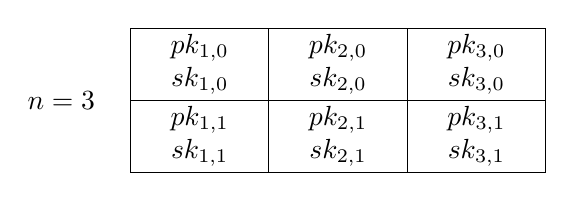
\begin{tikzpicture}
    \node [name=x, textnode] {$n = 3$}; 

    \node [name=ek10, rectanglenode, minimum width=5em, minimum height=2.6em, draw, 
        right of = x, xshift=5em, yshift=1.3em] {$pk_{1,0}$\\$sk_{1,0}$}; 
    \node [name=ek11, rectanglenode, minimum width=5em, minimum height=2.6em, draw, 
        right of = x, xshift=5em, yshift=-1.3em] {$pk_{1,1}$\\$sk_{1,1}$}; 

    \node [name=ek20, rectanglenode, minimum width=5em, minimum height=2.6em, draw, 
        right of = x, xshift=10em, yshift=1.3em] {$pk_{2,0}$\\ $sk_{2,0}$}; 
    \node [name=ek21, rectanglenode, minimum width=5em, minimum height=2.6em, draw, 
        right of = x, xshift=10em, yshift=-1.3em] {$pk_{2,1}$\\ $sk_{2,1}$}; 

    \node [name=ek30, rectanglenode, minimum width=5em, minimum height=2.6em, draw, 
        right of = x, xshift=15em, yshift=1.3em] {$pk_{3,0}$\\  $sk_{3,0}$}; 
    \node [name=ek31, rectanglenode, minimum width=5em, minimum height=2.6em, draw, 
        right of = x, xshift=15em, yshift=-1.3em] {$pk_{3,1}$\\$sk_{3,1}$}; 
\end{tikzpicture}
\end{center}
\caption{真实模式下$n=3$时密钥结构图示}
\end{figure}

\begin{figure}[!hbtp]
\begin{minipage}[t]{0.5\linewidth}
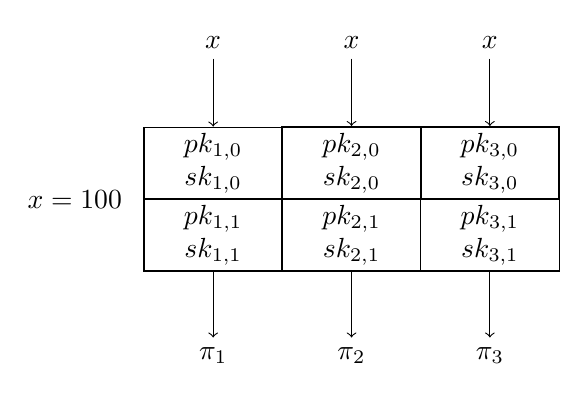
\begin{tikzpicture}
    \node [name=x, textnode] {$x = 100$}; 

    \node [name=ek10, rectanglenode, minimum width=5em, minimum height=2.6em, draw, 
        right of = x, xshift=5em, yshift=1.3em] {$pk_{1,0}$\\$sk_{1,0}$}; 
    \node [name=ek11, rectanglenode, minimum width=5em, minimum height=2.6em, draw, thick, 
        right of = x, xshift=5em, yshift=-1.3em] {$pk_{1,1}$\\$sk_{1,1}$}; 

    \node [name=ek20, rectanglenode, minimum width=5em, minimum height=2.6em, draw, thick,  
        right of = x, xshift=10em, yshift=1.3em] {$pk_{2,0}$\\ $sk_{2,0}$}; 
    \node [name=ek21, rectanglenode, minimum width=5em, minimum height=2.6em, draw, 
        right of = x, xshift=10em, yshift=-1.3em] {$pk_{2,1}$\\ $sk_{2,1}$}; 

    \node [name=ek30, rectanglenode, minimum width=5em, minimum height=2.6em, draw, thick,
        right of = x, xshift=15em, yshift=1.3em] {$pk_{3,0}$\\ $sk_{3,0}$}; 
    \node [name=ek31, rectanglenode, minimum width=5em, minimum height=2.6em, draw, 
        right of = x, xshift=15em, yshift=-1.3em] {$pk_{3,1}$\\$sk_{3,1}$}; 


    \node [name = x1, above of = ek10, yshift=1.5em] {$x$}; 
    \node [name = x2, above of = ek20, yshift=1.5em] {$x$}; 
    \node [name = x3, above of = ek30, yshift=1.5em] {$x$}; 

    \draw (x1) edge[->] (ek10); 
    \draw (x2) edge[->] (ek20); 
    \draw (x3) edge[->] (ek30); 

    \node [name = pi1, below of = ek11, yshift=-1.5em] {$\pi_1$}; 
    \node [name = pi2, below of = ek21, yshift=-1.5em] {$\pi_2$}; 
    \node [name = pi3, below of = ek31, yshift=-1.5em] {$\pi_3$}; 

    \draw (ek11) edge[->] (pi1); 
    \draw (ek21) edge[->] (pi2); 
    \draw (ek31) edge[->] (pi3); 
\end{tikzpicture}
\caption{真实模式下$x=010$时哈希证明计算图示}
\end{minipage}
\begin{minipage}[t]{0.5\linewidth}
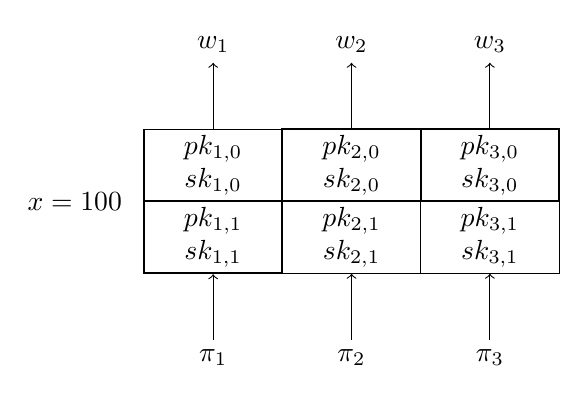
\begin{tikzpicture}
    \node [name=x, textnode] {$x = 100$}; 

    \node [name=ek10, rectanglenode, minimum width=5em, minimum height=2.6em, draw, 
        right of = x, xshift=5em, yshift=1.3em] {$pk_{1,0}$\\$sk_{1,0}$}; 
    \node [name=ek11, rectanglenode, minimum width=5em, minimum height=2.6em, draw, thick,
        right of = x, xshift=5em, yshift=-1.3em] {$pk_{1,1}$\\$sk_{1,1}$}; 

    \node [name=ek20, rectanglenode, minimum width=5em, minimum height=2.6em, draw, thick, 
        right of = x, xshift=10em, yshift=1.3em] {$pk_{2,0}$\\ $sk_{2,0}$}; 
    \node [name=ek21, rectanglenode, minimum width=5em, minimum height=2.6em, draw, 
        right of = x, xshift=10em, yshift=-1.3em] {$pk_{2,1}$\\ $sk_{2,1}$}; 

    \node [name=ek30, rectanglenode, minimum width=5em, minimum height=2.6em, draw, thick,
        right of = x, xshift=15em, yshift=1.3em] {$pk_{3,0}$\\  $sk_{3,0}$}; 
    \node [name=ek31, rectanglenode, minimum width=5em, minimum height=2.6em, draw, 
        right of = x, xshift=15em, yshift=-1.3em] {$pk_{3,1}$\\$sk_{3,1}$}; 


    \node [name = w1, above of = ek10, yshift=1.5em] {$w_1$}; 
    \node [name = w2, above of = ek20, yshift=1.5em] {$w_2$}; 
    \node [name = w3, above of = ek30, yshift=1.5em] {$w_3$}; 

    \draw (w1) edge[<-] (ek10); 
    \draw (w2) edge[<-] (ek20); 
    \draw (w3) edge[<-] (ek30); 

    \node [name = pi1, below of = ek11, yshift=-1.5em] {$\pi_1$}; 
    \node [name = pi2, below of = ek21, yshift=-1.5em] {$\pi_2$}; 
    \node [name = pi3, below of = ek31, yshift=-1.5em] {$\pi_3$}; 

    \draw (ek11) edge[<-] (pi1); 
    \draw (ek21) edge[<-] (pi2); 
    \draw (ek31) edge[<-] (pi3); 
\end{tikzpicture}
\caption{真实模式下$x=010$时证据提取图示}
\end{minipage}
\end{figure}

ABO-EHPS模拟模式下算法的正确性由DDN结构和EHPS对应算法保证. 
ABO-EHPS两种模式下公钥分布的统计不可区分性由EHPS两种模式下公钥分布的统计不可区分性与各公钥分量生成的独立性保证. 

\begin{figure}[!hbtp]
\begin{center}
\begin{tikzpicture}
    \node [name=xstar, textnode] {$x^* = 010$}; 

    \node [name=ek10, rectanglenode, minimum width=5em, minimum height=2.6em, draw, 
        right of = x, xshift=5em, yshift=1.3em] {$pk_{1,0}$\\\blue{$sk_{1,0}'$}}; 
    \node [name=ek11, rectanglenode, minimum width=5em, minimum height=2.6em, draw, 
        right of = x, xshift=5em, yshift=-1.3em] {$pk_{1,1}$\\$sk_{1,1}$}; 

    \node [name=ek20, rectanglenode, minimum width=5em, minimum height=2.6em, draw, 
        right of = x, xshift=10em, yshift=1.3em] {$pk_{2,0}$\\ $sk_{2,0}$}; 
    \node [name=ek21, rectanglenode, minimum width=5em, minimum height=2.6em, draw, 
        right of = x, xshift=10em, yshift=-1.3em] {$pk_{2,1}$\\\blue{$sk_{2,1}'$}}; 

    \node [name=ek30, rectanglenode, minimum width=5em, minimum height=2.6em, draw, 
        right of = x, xshift=15em, yshift=1.3em] {$pk_{3,0}$\\ \blue{$sk_{3,0}'$}}; 
    \node [name=ek31, rectanglenode, minimum width=5em, minimum height=2.6em, draw, 
        right of = x, xshift=15em, yshift=-1.3em] {$pk_{3,1}$\\$sk_{3,1}$}; 
\end{tikzpicture}
\end{center}
\caption{模拟模式下$n=3$, $x^*=010$时的密钥生成}
\end{figure}

\begin{figure}
\begin{minipage}[t]{0.5\linewidth}
\begin{tikzpicture}
    \node [name=x, textnode] {$x^* = 010$}; 

    \node [name=ek10, rectanglenode, minimum width=5em, minimum height=2.6em, draw, thick,  
        right of = x, xshift=5em, yshift=1.3em] {$pk_{1,0}$\\\blue{$sk_{1,0}'$}}; 
    \node [name=ek11, rectanglenode, minimum width=5em, minimum height=2.6em, draw, 
        right of = x, xshift=5em, yshift=-1.3em] {$pk_{1,1}$\\$sk_{1,1}$}; 

    \node [name=ek20, rectanglenode, minimum width=5em, minimum height=2.6em, draw, 
        right of = x, xshift=10em, yshift=1.3em] {$pk_{2,0}$\\ $sk_{2,0}$}; 
    \node [name=ek21, rectanglenode, minimum width=5em, minimum height=2.6em, draw, thick,  
        right of = x, xshift=10em, yshift=-1.3em] {$pk_{2,1}$\\ \blue{$sk_{2,1}'$}}; 

	\node [textnode, above of = ek20, yshift=6em] {不知晓随机数, 使用$\mathsf{PrivEval}(sk', x^*)$计算}; 

    \node [name=ek30, rectanglenode, minimum width=5em, minimum height=2.6em, draw, thick,
        right of = x, xshift=15em, yshift=1.3em] {$pk_{3,0}$\\ \blue{$sk_{3,0}'$}}; 
    \node [name=ek31, rectanglenode, minimum width=5em, minimum height=2.6em, draw, 
        right of = x, xshift=15em, yshift=-1.3em] {$pk_{3,1}$\\$sk_{3,1}$}; 

    \node [name = x1, above of = ek10, yshift=1.5em] {$x^*$}; 
    \node [name = x2, above of = ek20, yshift=1.5em] {$x^*$}; 
    \node [name = x3, above of = ek30, yshift=1.5em] {$x^*$}; 

    \draw (x1) edge[->] (ek10); 
    \draw (x2) edge[->] (ek20); 
    \draw (x3) edge[->] (ek30); 

    \node [name = pi1, below of = ek11, yshift=-1.5em] {$\pi_1^*$}; 
    \node [name = pi2, below of = ek21, yshift=-1.5em] {$\pi_2^*$}; 
    \node [name = pi3, below of = ek31, yshift=-1.5em] {$\pi_3^*$}; 

    \draw (ek11) edge[->] (pi1); 
    \draw (ek21) edge[->] (pi2); 
    \draw (ek31) edge[->] (pi3); 
\end{tikzpicture}
\caption{模拟模式下$x^* = 010$时哈希证明计算}
\end{minipage}
\begin{minipage}[t]{0.5\linewidth}
\begin{tikzpicture}
    \node [name=x, textnode] {$x=100$}; 

    \node [name=ek10, rectanglenode, minimum width=5em, minimum height=2.6em, draw,  
        right of = x, xshift=5em, yshift=1.3em] {$pk_{1,0}$\\\blue{$sk_{1,0}'$}}; 
    \node [name=ek11, rectanglenode, minimum width=5em, minimum height=2.6em, draw, thick,
        right of = x, xshift=5em, yshift=-1.3em] {$pk_{1,1}$\\$sk_{1,1}$}; 

    \node [name=ek20, rectanglenode, minimum width=5em, minimum height=2.6em, draw, thick,
        right of = x, xshift=10em, yshift=1.3em] {$pk_{2,0}$\\ $sk_{2,0}$}; 
    \node [name=ek21, rectanglenode, minimum width=5em, minimum height=2.6em, draw,  
        right of = x, xshift=10em, yshift=-1.3em] {$pk_{2,1}$\\ \blue{$sk_{2,1}'$}}; 
	\node [textnode, above of = ek20, yshift=6em] {知晓随机数, 使用$\mathsf{PubEval}(pk, x, r)$计算}; 

    \node [name=ek30, rectanglenode, minimum width=5em, minimum height=2.6em, draw, thick,
        right of = x, xshift=15em, yshift=1.3em] {$pk_{3,0}$\\ \blue{$sk_{3,0}'$}}; 
    \node [name=ek31, rectanglenode, minimum width=5em, minimum height=2.6em, draw, 
        right of = x, xshift=15em, yshift=-1.3em] {$pk_{3,1}$\\$sk_{3,1}$}; 

    \node [name = x1, above of = ek10, yshift=1.5em] {$x$}; 
    \node [name = x2, above of = ek20, yshift=1.5em] {$x$}; 
    \node [name = x3, above of = ek30, yshift=1.5em] {$x$}; 

    \draw (x1) edge[->] (ek10); 
    \draw (x2) edge[->] (ek20); 
    \draw (x3) edge[->] (ek30); 

    \node [name = pi1, below of = ek11, yshift=-1.5em] {$\pi_1$}; 
    \node [name = pi2, below of = ek21, yshift=-1.5em] {$\pi_2$}; 
    \node [name = pi3, below of = ek31, yshift=-1.5em] {$\pi_3$}; 

    \draw (ek11) edge[->] (pi1); 
    \draw (ek21) edge[->] (pi2); 
    \draw (ek31) edge[->] (pi3); 
\end{tikzpicture}
\caption{模拟模式下$x=100$时哈希证明计算}
\end{minipage}
\end{figure}

\begin{figure}[!hbtp]
\begin{center}
\begin{tikzpicture}
    \node [name=xstar, textnode] {$x^*=010$\\$x=100$}; 

    \node [name=ek10, rectanglenode, minimum width=5em, minimum height=2.6em, draw, 
        right of = x, xshift=5em, yshift=1.3em] {$pk_{1,0}$\\\blue{$sk_{1,0}'$}}; 
    \node [name=ek11, rectanglenode, minimum width=5em, minimum height=2.6em, draw, 
        right of = x, xshift=5em, yshift=-1.3em] {$pk_{1,1}$\\$sk_{1,1}$}; 

    \node [name=ek20, rectanglenode, minimum width=5em, minimum height=2.6em, draw, 
        right of = x, xshift=10em, yshift=1.3em] {$pk_{2,0}$\\ $sk_{2,0}$}; 
    \node [name=ek21, rectanglenode, minimum width=5em, minimum height=2.6em, draw,  
        right of = x, xshift=10em, yshift=-1.3em] {$pk_{2,1}$\\ \blue{$sk_{2,1}'$}}; 

    \node [name=ek30, rectanglenode, minimum width=5em, minimum height=2.6em, draw, 
        right of = x, xshift=15em, yshift=1.3em] {$pk_{3,0}$\\ \blue{$sk_{3,0}'$}}; 
    \node [name=ek31, rectanglenode, minimum width=5em, minimum height=2.6em, draw, 
        right of = x, xshift=15em, yshift=-1.3em] {$pk_{3,1}$\\$sk_{3,1}$}; 

    \node [name = w1, above of = ek10, yshift=1.5em] {$w_1$}; 
    \node [name = w2, above of = ek20, yshift=1.5em] {$w_2$}; 
    \node [name = x3, above of = ek30, yshift=1.5em] {$x$}; 

    \draw (w1) edge[<-] (ek10); 
    \draw (w2) edge[<-] (ek20); 
    \draw (x3) edge[->] (ek30); 

    \node [name = pi1, below of = ek11, yshift=-1.5em] {$\pi_1$}; 
    \node [name = pi2, below of = ek21, yshift=-1.5em] {$\pi_2$}; 
    \node [name = pi3, below of = ek31, yshift=-1.5em] {$\pi_3$}; 

    \draw (ek11) edge[<-] (pi1); 
    \draw (ek21) edge[<-] (pi2); 
    \draw (ek31) edge[->] (pi3); 

    \node [textnode, right of = x, xshift=30em] {$w_1 \leftarrow \text{EHPS}.\mathsf{Ext}(sk_{1,1}, \pi_1)$\\
    	$w_2 \leftarrow \text{EHPS}.\mathsf{Ext}(sk_{2,0}, \pi_2)$\\
    	check $w_1 \stackrel{?}{=} w_2$\\
    	check $\pi_3 \stackrel{?}{=} \text{EHPS}.\mathsf{PrivEval}(\blue{sk_{3,0}'}, x)$}; 
\end{tikzpicture}
\end{center}
\caption{模拟模式下$x=100$时证据提取过程}
\end{figure}

基于ABO-EHPS设计IND-CCA KEM的方式与构造~\ref{construction:CPA-KEM-from-EHPS}完全相同. 
KEM构造的正确性由ABO-EHPS的正确性和$\mathsf{R}_L$的单射性保证, 安全性由以下定理保证.  
\begin{theorem}
如果$\mathsf{R}_L$是单向的, 那么KEM是IND-CCA安全的.  
\end{theorem}

\begin{proof}
证明的思路仍然是首先由真实模式切换到模拟模式, 再在模拟模式下利用零知识性证明安全性. 
证明的要点是保证两种模式下对解密谕言机$\mathcal{O}_\text{decap}$回复的一致性. 
以下通过游戏序列完成定理证明:

\begin{trivlist}
\item $\text{Game}_0$: 对应真实的游戏. $\mathcal{CH}$在真实模式下运行ABO-EHPS与敌手$\mathcal{A}$交互. 
\begin{itemize}
\item 初始化: $\mathcal{CH}$计算$pp \leftarrow \mathsf{Setup}(1^\kappa)$, 
	\redul{$(pk, sk) \leftarrow \mathsf{KeyGen}(\lambda)$}, 将$pp$和$pk$发送$\mathcal{A}$. 

\item 挑战: $\mathcal{CH}$按照以下步骤生成挑战
    \begin{enumerate}
        \item 随机采样$(x^*, w^*) \leftarrow \mathsf{SampRel}(r^*)$;  
        \item 通过\redul{$\mathsf{PubEval}(pk, x^*, r^*)$}公开计算
        	$\pi^* \leftarrow \mathsf{H}_{pk}(x^*)$; 
        \item 计算$k_0^* \leftarrow \mathsf{hc}(w^*)$, 随机采样$k_1^* \sample K$; 
        \item 随机选取$\beta \sample \{0,1\}$, 将$(c^* = (x^*, \pi^*), k_\beta^*)$发送给$\mathcal{A}$作为挑战. 
    \end{enumerate}

\item 解封装询问$c = (x, \pi) \neq c^*$: 计算\redul{$w \leftarrow \mathsf{Ext}(sk, x, \pi)$}, 
    如果$(x, w) \in \mathsf{R}_L$则输出$\mathsf{hc}(w)$, 否则输出$\bot$.

\item 应答: $\mathcal{A}$输出对$\beta$的猜测$\beta'$, $\mathcal{A}$成功当且仅当$\beta'= \beta$.
\end{itemize}
为了利用ABO-EHPS的零知识性论证$\pi^*$和解封装询问不额外泄漏关于$w^*$的信息, 
需要将ABO-EHPS由真实模式切换到模拟模式. 为此, 先引入以下游戏作为过渡.

\item $\text{Game}_1$: 与$\text{Game}_0$完全相同, 
	惟一的区别是$\mathcal{CH}$将$(x^*, w^*) \leftarrow \mathsf{SampRel}(r^*)$由挑战阶段提前至初始化阶段. 
	显然, 该变化不会对敌手的视图有任何改变. 因此有:
	\begin{equation*}
    	\text{Game}_0 \equiv \text{Game}_1
	\end{equation*}

\item $\text{Game}_2$: 本游戏对解封装应答方式稍加改动, 以便于后续游戏将密文的ABO解封装询问转化为ABO-EHPS相对于$x^*$的ABO证据抽取. 
	对于解封装询问$c = (x, \pi) \neq c^*$, $\mathcal{CH}$应答如下: 
    \begin{itemize} 
        \item $x = x^* \wedge \pi \neq \pi^*$: 直接返回$\bot$.
        \item $x \neq x^*$: 计算$w \leftarrow \mathsf{Ext}(sk, x, \pi)$, 
        	如果$(x, w) \in \mathsf{R}_L$则返回$\mathsf{hc}(w)$, 否则返回$\bot$.  
    \end{itemize}
	由于$\mathsf{H}_{pk}$是确定性算法, 因此$\text{Game}_2$与$\text{Game}_1$中的解封装应答完全相同. 


\item $\text{Game}_3$: $\mathcal{CH}$在模拟模式下运行ABO-EHPS与敌手$\mathcal{A}$交互. 
\begin{itemize}
    \item 初始化: $\mathcal{CH}$与上一游戏的区别在于通过\redul{$(pk, sk') \leftarrow \mathsf{KeyGen}'(pp, x^*)$}生成密钥对.

    \item 挑战: $\mathcal{CH}$与上一游戏的区别在于通过\redul{$\mathsf{PrivEval}(sk', x^*)$} 
    	计算$\pi^* \leftarrow \mathsf{H}_{pk}(x^*)$.

    \item 解封装询问$c = (x, \pi) \neq c^*$: $\mathcal{CH}$应答如下
    \begin{itemize} 
        \item $x = x^* \wedge \pi \neq \pi^*$: 直接返回$\bot$.
        \item $x \neq x^*$: 计算\redul{$w \leftarrow \mathsf{Ext}'(sk', x, \pi)$}, 
        	如果$(x, w) \in \mathsf{R}_L$则返回$\mathsf{hc}(w)$, 否则返回$\bot$.
    \end{itemize}
\end{itemize}

\item 基于以下事实, 我们有: $\text{Game}_2 \approx_s \text{Game}_3$
\begin{itemize}
    \item $\mathsf{KeyGen}(pp)[1] \approx_s \mathsf{KeyGen}'(pp, x^*)[1]$
    
    \item $\mathsf{PubEval}(pk, x^*, r^*) = \mathsf{H}_{pk}(x^*) = \mathsf{PrivEval}(sk', x^*)$

    \item 对于解封装询问$c = (x, \pi)$: 当$x = x^*$时, 均返回$\bot$; 
    	当$x \neq x^*$时, ABO-EHPS真实模式和模拟模式的正确性以及解封装算法``提取-检验''的设计保证了应答一致. 
\end{itemize}
\end{trivlist}

\begin{claim}
如果$\mathsf{R}_L$是单向的, 那么$\AdvA^{\text{Game}_3} = \mathsf{negl}(\kappa)$. 
\end{claim}

\begin{proof}
证明思路是如果存在$\mathcal{A}$以不可忽略的优势赢得$\text{Game}_3$, 
那么可以构造出$\mathcal{B}$以不可忽略的优势打破$\mathsf{hc}$的伪随机性, 从而与$\mathsf{R}_L$的单向性假设冲突. 
给定关于$\mathsf{hc}$的伪随机性挑战$pp$和$(x^*, k_\beta^*)$, 其中$(x^*, w^*) \leftarrow \mathsf{SampRel}(r^*)$, 
$\mathcal{B}$模拟$\text{Game}_3$中的挑战者$\mathcal{CH}$与$\mathcal{A}$交互, 目标是猜测$\beta$. 
\begin{itemize}
    \item $\mathcal{B}$运行ABO-EHPS的模拟模式与$\mathcal{A}$进行交互, 其在初始化阶段不再采样$x^*$而是直接嵌入接收到的$x^*$, 
    	在挑战阶段将$\mathsf{hc}$的挑战$(x^*, k_\beta^*)$作为$\mathcal{A}$的KEM挑战. 
    	最终, $\mathcal{B}$输出$\mathcal{A}$的猜测$\beta'$. 
\end{itemize} 
容易验证, $\mathcal{B}$在$\text{Game}_3$中的模拟是完美的. 因此$\mathcal{B}$打破$\mathsf{hc}$伪随机性的优势与$\AdvA^{\text{Game}_3}$相同. 
断言得证! 
\end{proof}
综上, 定理得证!
\end{proof}

Wee~\cite{Wee-CRYPTO-2010}展示了ABO-EHPS蕴含ATDR.
\begin{construction}[基于ABO-EHPS的ATDR构造]
\begin{itemize}
\item $\mathsf{Setup}(1^\kappa)$: 运行$pp \leftarrow \text{ABO-EHPS}.\mathsf{Setup}(1^\kappa)$. 

\item $\mathsf{KeyGen}(pp)$: 运行$(pk, sk) \leftarrow \text{ABO-EHPS}.\mathsf{KeyGen}(pp)$, 
	令$pk$为求值公钥$ek$, $sk$为求逆陷门$td$. 

\item $\mathsf{Sample}(pk; r)$: 运行$(x, w) \leftarrow \mathsf{SampRel}(r)$, 
   	通过$\text{ABO-EHPS}.\mathsf{PubEval}(pk, x, r)$计算$\pi \leftarrow \mathsf{H}_{pk}(x)$, 输出$(w, (x, \pi))$.  

\item $\mathsf{TdInv}(td, (x, \pi))$: 计算$w \leftarrow \text{ABO-EHPS}.\mathsf{Ext}(sk, (x, \pi))$,  
    如果$(x, w) \in \mathsf{R}$则返回$w$, 否则返回$\bot$.
\end{itemize}
\end{construction}
上述ATDR构造的自适应单向性由ABO-EHPS的性质$\mathsf{R}_L$的单向性保证. 
该构造也在更抽象的层面解释了基于ABO-EHPS设计CCA安全KEM的实质是在构造ATDR.  


\subsection{小结}
EHPS的重要理论意义在于它阐释统一了一大类标准模型下的基于计算性假设的
IND-CCA PKE方案~\cite{Kiltz-PKC-2007, CKS-EUROCRYPT-2008, HK-EUROCRYPT-2009, HJKS-PKC-2010}. 
绝大多数标准模型下的PKE构造都可纳入EHPS和HPS的设计范式, 这也从公钥加密的角度再次证实了零知识证明的强大威力. 
目前尚未知晓如何基于lattice上的困难问题构造EHPS.   
\begin{center}
\begin{tikzpicture}
    \node [roundnode, name=EHPS, fill=blue!20, minimum height=2em, minimum width=5em] {EHPS};
    \node [textnode, name=CPAKEM, below of = EHPS, yshift=-6em] {IND-CPA KEM}; 
    \draw (EHPS) edge[->, thin] (CPAKEM);

    \node [roundnode, name=ABOEHPS, right of = EHPS, xshift=10em, fill=blue!60, minimum height=2em, minimum width=5em] {ABO-EHPS};
    \node [textnode, name=ATDR, below of = ABOEHPS, yshift=-3em] {ATDR};
    \node [textnode, name=CCAKEM, below of = ATDR, yshift=-3em] {IND-CCA KEM}; 
    \draw (ABOEHPS) edge[->, thin] (ATDR);
    \draw (ATDR) edge[->, thin] (CCAKEM);
    \draw (EHPS) edge[->, thin, color=red] node [above] {DDN} (ABOEHPS);

    \node [name=factoring, above of = ABOEHPS, xshift=-12em, yshift=6em, textnode] {\cite{HK-EUROCRYPT-2009}\\factoring};
    \node [name=CDH, above of = ABOEHPS, xshift=-6em, yshift=6em, textnode] {\cite{Kiltz-PKC-2007}\\gap-CDH};
    \node [name=twinCDH, above of = ABOEHPS, xshift=0em, yshift=6em, textnode] {\cite{CKS-EUROCRYPT-2008}\\twin CDH};
    \node [name=BCDH, above of = ABOEHPS, xshift=6em, yshift=6em, textnode] {\cite{HJKS-PKC-2010}\\BCDH};

    \draw (factoring) edge[->] (ABOEHPS);
    \draw (CDH) edge[->] (ABOEHPS);
    \draw (twinCDH) edge[->] (ABOEHPS);
    \draw (BCDH) edge[->] (ABOEHPS);

    \node[name=lattice, above of=ABOEHPS, textnode, xshift=12em, yshift=6em, color=gray] {lattice?};
    \draw (lattice) edge[->, color=gray] node[auto]{?} (ABOEHPS);
\end{tikzpicture}
\end{center}

\subsubsection{HPS与EHPS的分析比较}
\begin{trivlist}
\item 相同点
\begin{itemize}
    \item 均可看成指定验证者的零知识证明系统(DV-NIZK). 
    \item 证明的形式是哈希值.  
\end{itemize}

\item 不同点
\begin{itemize}
    \item HPS是标准的证明系统, 而EHPS是知识的证明系统. 

    \item HPS中哈希函数族$\mathsf{H}_{sk}$由私钥索引, EHPS中哈希函数族$\mathsf{H}_{pk}$有公钥索引. 

    \item 在基于HPS的PKE构造中, 密文$c$是实例$x$, 会话密钥$k$是证明$\pi$. 
    \begin{itemize}
        \item HPS的正确性保证了PKE的正确性 
        \item HPS的合理性(哈希函数的平滑性、一致性)与SMP问题的困难性保证了PKE的安全性, 
        	在证明过程中, 挑战实例需要从语言$L$上切换到语言外$X \backslash L$. 
    \end{itemize}

    \item 在基于EHPS的PKE构造中, 密文$c$由实例$x$和证明$\pi$组成, 会话密钥$k$是证据$w$.
    \begin{itemize}
        \item EHPS的知识提取性质保证了PKE的正确性
        \item EHPS的零知识性和二元关系的单向性保证了PKE的安全性, 在证明过程中, EHPS需要由真实模式切换为模拟模式. 
    \end{itemize}
\end{itemize}
\end{trivlist}

% \begin{frame}{Key Technique Towards CCA Security}
% \begin{itemize}
% \uncover<1->{
%     \item CPA game: $pk$ and $c^*$ do not leak $k^*$
% }
% \uncover<2->{
%     \item CCA game: $\mathcal{A}$ can query $\mathcal{O}_\mathsf{dec}$ with any $c \neq c^*$
% }

% \uncover<3->{
%     \item High-level strategy for CCA: \red{making $\mathcal{O}_\mathsf{dec}$ useless}
% }
% \end{itemize}

% \begin{columns}[onlytextwidth]
% \uncover<4->{
% \begin{column}{0.49\textwidth}
% \begin{tikzpicture}
%     \draw [color=black] (0,0) circle (1.5cm);
%     \draw (-1.5,1.5) node {$C$};
%     \draw (0,0) node [color=red] {$*$}; 

%     \draw (-0.8,0) node {\includegraphics [width=0.14in] {\path/Image/cartoon/smiley-face.png}};
%     \draw (0,0.8) node {\includegraphics [width=0.14in] {\path/Image/cartoon/smiley-face.png}};
%     \draw (-0.56,0.56) node {\includegraphics [width=0.14in] {\path/Image/cartoon/smiley-face.png}};
%     \draw (0,-0.8) node {\includegraphics [width=0.14in] {\path/Image/cartoon/smiley-face.png}};
%     \draw (-0.56,-0.56) node {\includegraphics [width=0.14in] {\path/Image/cartoon/smiley-face.png}};
%     \draw (0.56,-0.56) node {\includegraphics [width=0.14in] {\path/Image/cartoon/smiley-face.png}};
%     \draw (0.8,0) node {\includegraphics [width=0.14in] {\path/Image/cartoon/smiley-face.png}};
%     \draw (0.56,0.56) node {\includegraphics [width=0.14in] {\path/Image/cartoon/smiley-face.png}};
% \end{tikzpicture}
% \mdblue{All-But-One technique}\\ 
% make the rest ciphertexts independent of $c^*$: 
% $c \neq c^*$ are safe, e.g. ATDF, EHPS 
% \end{column}
% }

% \uncover<5->{
% \begin{column}{0.49\textwidth}
% \begin{tikzpicture}
%     \draw [color=black] (0,0) circle (1.5);
%     \draw (-1.5,1.5) node {$C$};
%     \draw (0,0) node [color=red] {$*$}; 
%     \draw (-0.8,0) node {\includegraphics [width=0.14in] {\path/Image/cartoon/smiley-face.png}};
%     \draw (0,0.8) node {\includegraphics [width=0.14in] {\path/Image/cartoon/smiley-face.png}};
%     \draw (-0.56,0.56) node {\includegraphics [width=0.12in] {\path/Image/cartoon/bomb-1.jpg}};
%     \draw (0,-0.8) node {\includegraphics [width=0.14in] {\path/Image/cartoon/smiley-face.png}};
%     \draw (-0.56,-0.56) node {\includegraphics [width=0.12in] {\path/Image/cartoon/bomb-1.jpg}};
%     \draw (0.56,-0.56) node {\includegraphics [width=0.12in] {\path/Image/cartoon/bomb-1.jpg}};
%     \draw (0.8,0) node {\includegraphics [width=0.14in] {\path/Image/cartoon/smiley-face.png}};
%     \draw (0.56,0.56) node {\includegraphics [width=0.12in] {\path/Image/cartoon/bomb-1.jpg}};
% \end{tikzpicture}
% \mdblue{Hard-to-Ask technique}\\ some of the rest ciphertexts are dangerous, 
% make $\mathcal{A}$ unable to generate one, e.g. HPS
% \end{column}
% }
% \end{columns}








\section{程序混淆类}
\begin{center}
    只要代码足够乱, 就没人能看得懂.  \\
                \hfill --- 防御性编程(代码混淆)
\end{center}

\subsection{背景知识}
程序混淆(program obfuscation)是一种编译的方法技术, 它将容易理解的源程序转化成难以理解的形式, 同时保持原有功能性不变. 
程序混淆概念起源于上世界70年代的代码混淆领域, 在软件保护领域(如软件水印、防逆向工程)有着广泛的应用, 然而一直缺乏严格的安全定义. 

\begin{figure}[!hbtp]
\begin{center}
\begin{tikzpicture}
    \node [name=C, textnode] {\includegraphics[width=1.2in]{figure/code.png}};
    \node [name=OC, textnode, right of=C, xshift=16em] {\includegraphics[width=1.2in]{figure/obf.png}};
    \draw (C) edge[->] node[above] {$\mathcal{O}$} (OC);
\end{tikzpicture}
\end{center}
\caption{程序混淆}
\end{figure}

Barak等~\cite{Barak-CRYPTO-2001}首次将程序混淆引入密码学领域, 将程序从狭义的代码泛化为广义的算法, 
同时提出了虚拟黑盒(VBB, virtual black-box)混淆的严格定义. 

\begin{figure}[!hbtp]
\begin{center}
\begin{tikzpicture}
    \node [rectanglenode, name=C, minimum width=6em, minimum height=3em] {$C$};
    \node [name=OC, rectanglenode, fill=gray, right of=C, xshift=12em, minimum width=6em, minimum height=3em] {~$\mathcal{O}(C)$~};
    \node [name=BC, rectanglenode,  fill=black, below of=OC, yshift=-6em, minimum width=6em, minimum height=3em] {};
    \draw (C) edge[->] node[above] {$\mathcal{O}$} (OC);
    \node [textnode, below of=OC, yshift=-3em] {$\approx_c$};
\end{tikzpicture}
\end{center}
\caption{虚拟黑盒混淆}
\end{figure}

我们回顾不可区分混淆(indistinguishability obfuscator, $\iO$)~\cite{Garg-FOCS-2013}如下. 
\begin{definition}[虚拟黑盒混淆]
我们称一个uniform PPT machine $\iO$是电路簇$\{\mathcal{C}_\kappa\}$的不可区分混淆器当且仅当其满足以下两个条件:
\begin{itemize}
\item 功能保持: 对于任意安全参数$\kappa \in \mathbb{N}$、任意的$C \in \mathcal{C}_\kappa$和所有输入$x \in \{0,1\}^*$有:
    \begin{equation*}
        \Pr[C'(x) = C(x): C' \leftarrow \iO(\kappa, C)] = 1
    \end{equation*} 

\item 虚拟黑盒混淆: 存在PPT的模拟器$\mathcal{S}$, 对于任意$C \in \{\mathcal{C}_\kappa\}$, 对于任意PPT敌手$\mathcal{A}$, 
	我们有: 
    \begin{equation*}
        \mathcal{A}(\mathcal{O}(C)) \approx_c \mathcal{S}^{C}
    \end{equation*}   
    其中公式左边表示$\mathcal{A}$的视图, 公式右边表示$\mathcal{S}$在通过对$C$进行黑盒访问所输出的视图. 
\end{itemize} 
\end{definition}

\begin{note}
虚拟黑盒混淆的定义是基于模拟的游戏, 刻画的是PPT敌手从混淆程序$\mathcal{O}(C)$中获取的任何信息不会比黑盒访问$C$获得的信息更多. 
换言之, 掌握$\mathcal{O}(C)$的敌手视图可以由模拟器通过黑盒访问$C$模拟得出. 
VBB试图隐藏程序$C$的所有细节. 比如$C$以平方差公式计算$x^2-1$, 即$C(x) = (x+1)(x-1)$. 
那么敌手在获得$\mathcal{O}(C)$后, 掌握的所有信息等价输入/输出元组$(x, x^2-1)$, i.e., $(1, 0)$, $(2, 3)$, $(3, 8)$, $\dots$
\end{note}

VBB的混淆定义强到极致, 因此在密码学中应用起来颇为简单直观. 
事实上, 在1976年Diffie和Hellman的划时代论文~\cite{DH-IEEE-IT-1976}中, 
就已经提出了利用混淆器将对称加密方案编译为公钥加密方案的想法(如图~\ref{figure:Diffie-Hellman-idea}): 
\begin{enumerate}
    \item 将对SKE的加密算法$\mathsf{Enc}(sk, m, r)$中的第一个输入hardwired进电路, 得到$\mathsf{Enc}_{sk}(m, r)$; 
    \item 利用混淆器编译$\mathsf{Enc}_{sk}(\cdot, \cdot)$, 将得到的混淆程序作为公钥$pk$.
\end{enumerate}

\begin{figure}[!hbtp]
\begin{center}
\begin{tikzpicture}
    \node [rectanglenode, name=enc, minimum width=5em, minimum height=2em] {$\mathsf{Enc}$};
    \node [textnode, name=sk, above of=enc, xshift=-3em, yshift=3em, color=red] {$sk$}; 
    \node [textnode, name=m, above of=enc, xshift=0em, yshift=3em] {$m$}; 
    \node [textnode, name=r, above of=enc, xshift=3em, yshift=3em] {$r$};
    \node [textnode, name=c, below of=enc, yshift=-3em] {$c$}; 
    \draw (sk) edge[->] (enc);
    \draw (m) edge[->]  (enc);
    \draw (r) edge[->]  (enc);
    \draw (enc) edge[->] (c);

    \node [rectanglenode, name=dec, right of=enc, xshift=16em, minimum width=5em, minimum height=2em] {$\mathsf{Dec}$};
    \node [textnode, name=sk1, above of=dec, xshift=-3em, yshift=3em, color=red] {$sk$}; 
    \node [textnode, name=c1, above of=dec, xshift=3em, yshift=3em] {$c$}; 
    \node [textnode, name=m1, below of=dec, yshift=-3em] {$m$}; 
    \draw (sk1) edge[->] (dec);
    \draw (c1) edge[->]  (dec);
    \draw (dec) edge[->] (m1);

    \node [rectanglenode, name=enc2, below of=enc, yshift=-12em, minimum width=5em, minimum height=2em] {$\mathsf{Enc}_{\red{sk}}$}; 
    \node [textnode, name=m2, above of=enc2, xshift=-3em, yshift=3em] {$m$}; 
    \node [textnode, name=r2, above of=enc2, xshift=3em, yshift=3em] {$r$};
    \node [textnode, name=c2, below of=enc2, yshift=-3em] {$c$}; 
    \draw (m2) edge[connect]  (enc2);
    \draw (r2) edge[connect]  (enc2);
    \draw (enc2) edge[connect] (c2);

    \draw (sk) edge[->, bend left=-45] node[right] {hardwired} (enc2.west);

    \node [rectanglenode, fill = gray, name=enc3, right of=enc2, xshift=16em, minimum width=5em, minimum height=2em] 
        {$\mathcal{O}(\mathsf{Enc}_{sk})$}; 
    \node [textnode, name=m3, above of=enc3, xshift=-3em, yshift=3em] {$m$}; 
    \node [textnode, name=r3, above of=enc3, xshift=3em, yshift=3em] {$r$};
    \node [textnode, name=c3, below of=enc3, yshift=-3em] {$c$}; 
    \draw (m3) edge[->]  (enc3);
    \draw (r3) edge[->]  (enc3);
    \draw (enc3) edge[->] (c3);

    \node [textnode, name=pk, right of=enc3, xshift=5em] {$pk$}; 
    \draw (enc3) edge[->] (pk);

    \draw (enc2) edge[->] node[above] {obfuscate} (enc3);
\end{tikzpicture}
\end{center}
\caption{SKE $\Rightarrow$ PKE via obfuscation}\label{figure:Diffie-Hellman-idea}
\end{figure}

VBB的安全定义至强, Barak等~\cite{Barak-CRYPTO-2001}指出VBB``too good to be true!''--不存在针对任意电路(通用, general-purpose)的VBB. 
VBB因为安全太强以至于不存在, Garg等~\cite{Garg-FOCS-2013}降低了安全性要求, 引入了不可区分混淆(indistinguishability obfuscator, $\iO$). 
\begin{definition}[不可区分混淆($\iO$)]
我们称一个uniform PPT machine $\iO$是电路簇$\{\mathcal{C}_\kappa\}$的不可区分混淆器当且仅当其满足以下两个条件:
\begin{itemize}
\item 功能保持: 对于任意安全参数$\kappa \in \mathbb{N}$、任意的$C \in \mathcal{C}_\kappa$和所有输入$x \in \{0,1\}^*$有:
    \begin{equation*}
        \Pr[C'(x) = C(x): C' \leftarrow \iO(\kappa, C)] = 1
    \end{equation*} 

\item 不可区分混淆: 对于任意PPT敌手$(\mathcal{S}, \mathcal{D})$, 存在关于安全参数的可忽略函数$\alpha$使得: 
    如果$\Pr[\forall x, C_0(x) = C_1(x): (C_0, C_1, aux) \leftarrow \mathcal{S}(\kappa)] \geq 1 - \alpha(\kappa)$, 
    那么我们有: 
    \begin{equation*}
        \left|\Pr[\mathcal{D}(aux, \iO(\kappa, C_0)) = 1] - 
        \Pr[\mathcal{D}(aux, \iO(\lambda, C_1)) = 1]\right| \leq \alpha(\kappa)
    \end{equation*}   
\end{itemize} 
\end{definition}

\begin{figure}[!hbtp]
\begin{center}
\begin{tikzpicture}
    \node [rectanglenode, name=C0, minimum width=6em, minimum height=3em] {$C_0$};
    \node [name=C1, rectanglenode, below of=C0, minimum width=6em, minimum height=3em, yshift=-8em] {$C_1$};
    \node [name=OC0, rectanglenode,  fill=gray, right of=C0, xshift=12em, minimum width=6em, minimum height=3em] {$\iO(C_0)$};
    \node [name=OC1, rectanglenode, fill=gray, right of=C1, xshift=12em, minimum width=6em, minimum height=3em] {$\iO(C_1)$};
    \draw (C0) edge[->] node[above] {$\iO$} (OC0);
    \draw (C1) edge[->] node[above] {$\iO$} (OC1);
    \node [textnode, below of=C0, yshift=-4em] {$\equiv$};
    \node [textnode, below of=OC0, yshift=-4em] {$\approx_c$};
\end{tikzpicture}
\end{center}
\caption{不可区分混淆示意图}
\end{figure}


\begin{remark}
\begin{itemize}
\item 不可区分混淆的定义类似加密方案的不可区分性, 对于任意功能相同的电路$C_0$和$C_1$, 均有$\iO(C_0) \approx_c \iO(C_1)$. 
    这里, 我们可以把电路$C$类比为消息, $\iO$类比为加密算法. 与VBB试图隐藏电路的所有信息不同, 
    $\iO$只试图隐藏电路的部分信息: 比如$C_0(x) = (x+1)(x-1)$, $C_1(x) = (x+2)(x-2)+3$,    
    那么如果混淆后的程序均是$x^2-1$即可满足不可区分安全性.
    非严格的说, $\iO$试图在以统一的方式完成同质的计算. 

\item 在上述定义中, 条件\redul{$\Pr[\forall x, C_0(x) = C_1(x): (C_0, C_1, aux) \leftarrow \mathcal{S}(\kappa)] \geq 1 - \alpha(\kappa)$}
    并不意味着$C_0$和$C_1$存在差异输入(differing-inputs), 而指的是$C_0$和$C_1$以极高的概率功能性完全相同, 
    这一点体现在概率空间定义在$\mathcal{S}$的随机带而与$x$无关. 

\item $aux$表示$\mathcal{S}$在采样$C_0, C_1$过程中得到的任意信息, 用于辅助$\mathcal{D}$区分$\iO(C_0)$和$\iO(C_1)$. 
\end{itemize}
\end{remark}

\begin{trivlist}
\item \textbf{差异输入混淆.} 如果在上述$\iO$定义中, 将$\mathcal{S}$所采样两个电路的要求由功能性完全相同放宽为允许存在差异输入, 
    则得到的是更强的混淆器, 称为差异输入混淆($\diO$, differing-input obfuscation). 
    \cite{BCP-TCC-2014}中给出了正面结果: 证明了$\iO$蕴含多项式级别差异输入规模的$\diO$. 
    \cite{BSW-EUROCRYPT-2016}中给出了负面结果: 证明了亚指数安全(sub-exponentially secure)的单向函数存在, 
    则针对无界输入Turing machine(TMs with unbounded inputs)亚指数安全的$\diO$不存在.  
\end{trivlist}

我们再把注意力转回不可区分混淆. 如上所述, VBB易用但对于通用电路并不存在, $\iO$弱化了安全要求, 从而有了基于合理困难性假设的构造. 
安全性弱化后$\iO$是否还有着强大的威力? 如何去应用呢? 
直观上: 混淆后的程序既可以保持功能性, 又能够在某种程度上隐藏常量. 
常量皆程序. 在密码学中, 公钥和私钥均可以看做一段程序, 其中硬编码(hardwired)原本的公钥和私钥作为常量: 比如加密就是以明文和随机数为输入, 运行``公钥程序'', 输出密文; 
解密就是以密文为输入, 运行``解密程序'', 输出明文. 
混淆在密码学中的一类强大应用就是完成从Minicrypt到Cryptomania的穿越, 因为借助混淆, 可以在不泄漏秘密的情况下以公开的方式执行某个任务.  
\begin{itemize}
    \item 保持功能性 $\Rightarrow$ 确保密码方案的功能性
    \item 在某种程度上隐藏常量(对应需要保护的秘密) $\Rightarrow$ 确保密码方案的安全性
\end{itemize}

\begin{remark}
混淆的威力强大如魔法, 其力量的来源在于对底层密码组件的调用方式是非黑盒的(non-black-box), 因此可以绕过黑盒意义下的不可能结果(black-box impossibilities). 
\end{remark}

在$\iO$提出后最初的一段时间, 应用只局限于属性加密(ABE). 
原因是应用$\iO$设计密码方案并非易事, 需要解决的技术难题是精准的隐藏``部分信息''. 
2014年, Sahai和Waters~\cite{SW-STOC-2014}创造性的发展了可穿孔编程技术(puncture program technique), 
以此给出了应用$\iO$的范式, 展示了$\iO$的巨大威力--结合单向函数和$\iO$重构了几乎所有的密码组件, 
包括公钥加密/密钥封装、可否认加密、数字签名、单向陷门函数、非交互式零知识证明、不经意传输等.

\subsection{受限伪随机函数}
以下首先介绍可穿孔编程技术的关键密码组件---受限伪随机函数(constrained PRF). 
对于标准的伪随机函数$F: K \times X \rightarrow Y$, 密钥$k$不支持代理, 因此求值方式是``完全或无''(all-or-nothing):
\begin{itemize}
    \item 知晓密钥$k$时, 可以对定义域中的所有点$x \in X$进行函数求值, 得到$F_k(x)$.
    \item 不知晓密钥$k$时, $F_k(\cdot)$是伪随机的. 
\end{itemize}

三组科学家~\cite{BW-ASIACRYPT-2013, KPTZ-CCS-2013, BGI-PKC-2014}独立并行的提出了受限伪随机函数(constrained PRF). 
在受限伪随机函数中, $k$可以进一步代理得到受限密钥, 受限密钥可以对定义域中的部分输入进行求值. 正式的定义如下: 
\begin{definition}[受限伪随机函数(constrained PRF)] 
受限伪随机函数包含以下多项式时间算法: 
\begin{itemize}
\item $\mathsf{Setup}(1^\kappa)$: 以安全参数为输入, 输出公开参数$pp$, 其中包含了函数$F: K \times X \rightarrow Y$的描述
    以及电路族$\mathcal{C} = \{f: X \rightarrow \{0,1\}\}$的描述. 

\item $\mathsf{KeyGen}(pp)$: 随机采样密钥$k \sample K$. 

\item $\mathsf{Constrain}(k, f)$: 以密钥$k$和$c \in \mathcal{C}$为输入, 输出受限密钥$k_f$. 

\item $\mathsf{Eval}(k/k_f, x) = F_k(x)$: 以密钥$k$或受限密钥$k_c$和$x \in X$为输入, 当第一输入为$k$时输出$F_k$, 
    当第一输入为$k_c$时, 如果$f(x)=1$则输出$F_k(x)$, 否则输出$\bot$. 
\end{itemize}
\end{definition}

\begin{trivlist}
\item \textbf{安全性.} 受限伪随机函数要求对于没有被受限密钥和求值询问覆盖的输入, 其输出仍然是伪随机的. 
    定义敌手$\mathcal{A} = (\mathcal{A})$的优势函数如下: 
\begin{displaymath}
    \Pr \left[\beta = \beta': 
    \begin{array}{l}
        pp \leftarrow \mathsf{Setup}(1^\lambda); \\
        k \leftarrow \mathsf{KeyGen}(pp); \\
        (x^*, state) \leftarrow \mathcal{A}_1^{\Oeval, \Oconstrain}(pp);\\
        \beta \sample \{0, 1\}, y_0^* = F_k(x^*), y_1^* \sample Y; \\
        \beta' \leftarrow \mathcal{A}_2^{\Oeval, \Oconstrain}(state, y_\beta^*);
    \end{array}
    \right] - \frac{1}{2}.
\end{displaymath}
其中$\Oeval$表示求值谕言机, 以$x \in X$为输入, 返回$F_k(x)$; 
$\Oconstrain$表示受限密钥谕言机, 以$c \in \mathcal{C}$为输入, 输出$k_c$. 
在安全试验过程中, 挑战者隐式的维护集合$H$以记录被已发起的受限密钥询问和求值询问覆盖的定义域中元素.  
为了避免定义无意义, $\mathcal{A}_1$在第一阶段被禁止选择$H$中的元素作为挑战点, 
$\mathcal{A}_2$在第二阶段被禁止发起能够覆盖挑战点的受限密钥询问和求值询问. 
如果任意的PPT敌手$\mathcal{A}$在上述游戏中的优势函数均为可忽略函数, 则称受限伪随机函数是安全的. 
\end{trivlist}

\begin{remark}
对任意$\mathcal{C}$, 均存在平凡的受限伪随机函数构造: 受限密钥生成函数通过枚举的方式生成受限密钥, 即$k_f = \{y = F_k(x)\}_{f(x)=1}$. 
为了排除此类平凡的构造, 我们要求受限密钥是紧致的, 即对于$\forall f \in \mathcal{C}$, 均有$|k_f| = \kappa^{O(1)}$. 
\end{remark}

Sahai和Waters~\cite{SW-STOC-2014}引入了受限伪随机函数的特例——可穿孔伪随机函数(puncturable PRF), 正式定义如下: 
\begin{definition}[可穿孔伪随机函数(puncturable PRF)] 
可穿孔伪随机函数包含以下多项式时间算法: 
\begin{itemize}
\item $\mathsf{Setup}(1^\kappa)$: 以安全参数为输入, 输出公开参数$pp$, 其中包含了函数$F: K \times X \rightarrow Y$的描述
    和电路族$\mathcal{C} = \{f_{x^*}: X \rightarrow \{0,1\}\}_{x^* \in X}$的描述.  
    $f_{x^*}(\cdot)$的具体定义是$f_{x^*}(x) = \neg x^* \stackrel{?}{=}x$. 为了表述简洁, 以下在不引起混淆的情况下使用$x^*$表征$f_{x^*}$.   

\item $\mathsf{KeyGen}(pp)$: 随机采样密钥$k \sample K$. 

\item $\mathsf{Puncture}(k, x^*)$: 以密钥$k$和$x^* \in X$为输入, 输出受限密钥$k_{x^*}$. 

\item $\mathsf{Eval}(k/k_{x^*}, x)$: 以密钥$k$或受限密钥$k_{x^*}$和$x \in X$为输入, 当第一输入为$k$时输出$F_k$, 
    当第一输入为$k_{x^*}$时, 如果$x \neq x^*$时输出$F_k(x)$, 否则输出$\bot$. 
\end{itemize}
\end{definition}

可穿孔伪随机函数的安全定义直觉是对于没有被受限密钥覆盖的输入, 其输出仍然是伪随机的. 存在以下两种等价定义. 
\begin{trivlist}
\item \textbf{选择伪随机性.} 定义敌手$\mathcal{A} = (\mathcal{A}_1, \mathcal{A}_2)$的优势函数如下: 
\begin{displaymath}
    \Pr \left[\beta = \beta': 
    \begin{array}{l}
        (x^*, state) \leftarrow \mathcal{A}_1(\kappa);\\
        pp \leftarrow \mathsf{Setup}(1^\lambda); \\
        k \leftarrow \mathsf{KeyGen}(pp); \\
        k_{x^*} \leftarrow \mathsf{Puncture}(k, x^*);\\ 
        \beta \sample \{0, 1\}, y_0^* = F_k(x^*), y_1^* \sample Y; \\
        \beta' \leftarrow \mathcal{A}_2(state, k_x^*, y_\beta^*);
    \end{array}
    \right] - \frac{1}{2}.
\end{displaymath}
如果任意的PPT敌手$\mathcal{A}$在上述游戏中的优势函数均为可忽略函数, 则称可穿孔伪随机函数是选择伪随机的. 
\end{trivlist}

\begin{figure}[!hbtp]
\begin{center}
\begin{tikzpicture}
    \node [name=adv, textnode] {\includegraphics[width=0.5in]{figure/adversary.png}};
    \node [name=challenger, textnode, right of = adv, xshift=18em] 
        {\includegraphics[width=0.5in]{figure/challenger.png}}; 

    \draw ($(adv.east)+(0em, 0.5em)$) edge[->] node[above] {$x^*$} ($(challenger.west)+(0em, 0.5em)$);

    \node [name=setup, textnode, right of=challenger, xshift = 9em, yshift = 1.5em] 
         {$pp \leftarrow \mathsf{Setup}(1^\kappa)$\\$k \sample K$, $\beta \sample \{0,1\}$\\$k_{x^*} \leftarrow \mathsf{Puncture}(k, x^*)$
         \\$y_0^* \leftarrow F(k, x^*)$; $y_1^* \sample Y$}; 
    \draw ($(challenger.west)+(0em, -1.5em)$) edge[->] node[above] {$pp$, $k_{x^*}$, $y_\beta^*$} ($(adv.east)+(0em, -1.5em)$);

    \draw ($(adv.east)+(0em, -3em)$) edge[->] node[above] {$\beta'$} ($(challenger.west)+(0em, -3em)$);
    \node [name=win, textnode, right of=challenger, xshift = 6.5em, yshift = -3em] {$\beta' = ? \beta$}; 
\end{tikzpicture}
\end{center}
\caption{可穿孔伪随机函数选择伪随机性示意图}
\end{figure}

\begin{trivlist}
\item \textbf{弱伪随机性.} 定义敌手$\mathcal{A} = (\mathcal{A}_1, \mathcal{A}_2)$的优势函数如下: 
\begin{displaymath}
    \Pr \left[\beta = \beta': 
    \begin{array}{l}
        pp \leftarrow \mathsf{Setup}(1^\lambda); \\
        k \leftarrow \mathsf{KeyGen}(pp), x^* \sample X; \\
        k_{x^*} \leftarrow \mathsf{Puncture}(k, x^*);\\ 
        \beta \sample \{0, 1\}, y_0^* = F_k(x^*), y_1^* \sample Y; \\
        \beta' \leftarrow \mathcal{A}(pp, x^*, k_x^*, y_\beta^*);
    \end{array}
    \right] - \frac{1}{2}.
\end{displaymath}
如果任意的PPT敌手$\mathcal{A}$在上述游戏中的优势函数均为可忽略函数, 则称可穿孔伪随机函数是弱伪随机的. 
\end{trivlist}

\begin{figure}[!hbtp]
\begin{center}
\begin{tikzpicture}
    \node [name=adv, textnode] {\includegraphics[width=0.5in]{figure/adversary.png}};
    \node [name=challenger, textnode, right of = adv, xshift=18em] 
        {\includegraphics[width=0.5in]{figure/challenger.png}}; 

    \draw ($(adv.east)+(0em, 0.5em)$) edge[<-] node[above] {$pp, x^*, k_{x^*}, y_\beta$} ($(challenger.west)+(0em, 0.5em)$);

    \node [name=setup, textnode, right of=challenger, xshift = 9em, yshift = 1.5em] 
         {$pp \leftarrow \mathsf{Setup}(1^\kappa)$\\$k \sample K$, $\beta \sample \{0,1\}$\\$x^* \sample X$, $k_{x^*} \leftarrow \mathsf{Puncture}(k, x^*)$
         \\$y_0^* \leftarrow F(k, x^*)$; $y_1^* \sample Y$}; 
    \draw ($(adv.east)+(0em, -1.5em)$)  edge[->] node[above] {$\beta'$} ($(challenger.west)+(0em, -1.5em)$);

    \node [name=win, textnode, right of=challenger, xshift = 6.5em, yshift = -3em] {$\beta' = ? \beta$}; 
\end{tikzpicture}
\end{center}
\caption{可穿孔伪随机函数弱伪随机性示意图}
\end{figure}
文献~\cite{Chen-ASIACRYPT-2018}证明了可穿孔弱伪随机函数的两种安全定义等价. 

\begin{remark}
在定义方面, 可穿孔伪随机函数中的受限密钥$k_{x^*}$求值功能是``全除一''的, 是ABO类型密钥. 
在安全性方面, 可穿孔伪随机函数要求弱伪随机性, 
即对于挑战者随机选择的点$x^*$, 即使拥有$k_x^*$, $F(x^*)$在敌手的视图中依然伪随机, 即: 
\begin{equation*}
     (pp, x^*, k_{x^*}, \red{F_k(x^*)}) \approx_c (pp, x^*, k_{x^*}, y^*), \text{其中~}y^* \sample Y
\end{equation*}

由于可穿孔伪随机函数的受限类型特殊, 因此安全定义相比一般的受限伪随机函数在形式上更加简单. 
\end{remark}

可穿孔伪随机函数可以通过GGM树形伪随机函数自然得出~\cite{BW-ASIACRYPT-2013, KPTZ-CCS-2013, BGI-PKC-2014}, 因此仍属于Minicrypt. 

\begin{figure}[!hbtp]
\begin{center}
\begin{tikzpicture}
% draw the root
\node [rectanglenode, dashed, name=root, minimum width=4em, minimum height=2em] {$s$};

% layer 1 
\node [rectanglenode, name=s0, dashed, below of=root, yshift=-5em, xshift=-8em, minimum width=4em, minimum height=2em] {$\mathsf{G}_0(s)$}; 
\node [rectanglenode, name=s1, below of=root, yshift=-5em, xshift=8em, minimum width=4em, minimum height=2em] {$\mathsf{G}_1(s)$}; 

% layer 2
\node [rectanglenode, name=s00, below of=s0, xshift=-5em, yshift=-5em, minimum width=4em, minimum height=2em] {$\mathsf{G}_0(\mathsf{G}_0(s))$}; 
\node [rectanglenode, name=s01, below of=s0, dashed, xshift=3.5em, yshift=-5em, minimum width=4em, minimum height=2em] {$\mathsf{G}_1(\mathsf{G}_0(s))$}; 

\node [rectanglenode, name=s10, below of=s1, xshift=-3.5em, yshift=-5em, minimum width=4em, minimum height=2em] {}; 
\node [rectanglenode, name=s11, below of=s1, xshift=5em, yshift=-5em,  minimum width=4em, minimum height=2em] {}; 

% leaf
\node [circlenode, name=l000, below of=s00, xshift=-2.2em, yshift=-5em, minimum width=2em] {}; 
\node [circlenode, name=l001, below of=s00, xshift=2.2em, yshift=-5em, minimum width=2em] {}; 

\node [circlenode, draw=blue!30, fill=blue!30, name=l010, below of=s01, xshift=-2.2em, yshift=-5em, minimum width=2em] {}; 
\node [textnode, name=l011, below of=s01, xshift=2.2em, yshift=-5em, minimum width=2em] {$\mathsf{G}_1(\mathsf{G}_1(\mathsf{G}_0(s)))$}; 

\node [circlenode, name=l100, below of=s10, xshift=-2.2em, yshift=-5em, minimum width=2em] {}; 
\node [circlenode, name=l101, below of=s10, xshift=2.2em, yshift=-5em, minimum width=2em] {}; 

\node [circlenode, name=l110, below of=s11, xshift=-2.2em, yshift=-5em, minimum width=2em] {}; 
\node [circlenode, name=l111, below of=s11, xshift=2.2em, yshift=-5em, minimum width=2em] {}; 


% arrows
\draw (root.south) edge[->, thick, red] node [above] {0} (s0.north);
\draw (root.south) edge[->, thin] (s1.north);

\draw (s0.south) edge[->, thin] (s00.north);
\draw (s0.south) edge[->, thick, red] node [above, xshift=0.4em, yshift=-0.5em] {1} (s01.north);
\draw (s1.south) edge[->, thin] (s10.north);
\draw (s1.south) edge[->, thin] (s11.north);

\draw ($(s00.south)$) edge[->, thin] (l000);
\draw ($(s00.south)$) edge[->, thin] (l001);
\draw ($(s01.south)$) edge[->, thick, red] node [above, xshift=-0.4em, yshift=-0.5em] {0} (l010);
\draw ($(s01.south)$) edge[->, thin] (l011);
\draw ($(s10.south)$) edge[->, thin] (l100);
\draw ($(s10.south)$) edge[->, thin] (l101);
\draw ($(s11.south)$) edge[->, thin] (l110);
\draw ($(s11.south)$) edge[->, thin] (l111);


\node [textnode, name=l0, right of = root, xshift=20em] {$0$}; 
\node [textnode, name=l1, below of = l0, yshift=-5em] {$1$}; 
\node [textnode, name=l2, below of = l1, yshift=-5em] {$2$}; 
\node [textnode, name=ln, below of = l2, yshift=-5em] {$3$}; 

\end{tikzpicture}
\end{center}
\caption{GGM construction: $k_{010} = \{\mathsf{G}_0(\mathsf{G}_0(s)), 
\mathsf{G}_1(\mathsf{G}_0(\mathsf{G}_0(s))), \mathsf{G}_1(s)\}$}
\end{figure}


\subsection{基于不可区分混淆的KEM构造}
本章将逐步的展示如何基于$\iO$构造KEM, 实现Diffie-Hellman当年的梦想. 

\begin{trivlist}
    \item \textbf{起点方案.} 首先将对称场景下基于PRF的KEM封装算法表达为程序的形式, 如下图所示.
\end{trivlist}

\begin{framed}
\vspace{-1em}
\begin{center}$\mathsf{Encaps}$\end{center}
\vspace{-1em}
\begin{trivlist}   
    \item Input: secret key {$\boxed{sk}$}, randomness $x$ 
        \begin{enumerate}\itemsep 1pt \parskip 0pt \parsep 0pt
            \item output $c = x$, $k \leftarrow \mathsf{PRF}(sk, c)$.
        \end{enumerate}
\end{trivlist}
\vspace{-1em}
\end{framed}
再对程序进行微调, 将$sk$由输入变为hardwired的常量, 如下图所示:  

\begin{framed}
\vspace{-1em}
\begin{center}$\mathsf{Encaps}$\end{center}
\begin{trivlist}
    \item \underline{Constants: secret key {$sk$}} 
    \item Input: randomness $x$ 
        \begin{enumerate}\itemsep 1pt \parskip 0pt \parsep 0pt
            \item output $c = x$, $k \leftarrow F(sk, c)$.
        \end{enumerate}
\end{trivlist}
\vspace{-1em}
\end{framed}

由于通用的VBB并不存在, 因此尝使用$\iO$对程序混淆, 将混淆后的结果作为公钥
\begin{equation*}
    pk \leftarrow \red{\iO}(\mathsf{Encaps})
\end{equation*}

\begin{trivlist}
\item \textbf{技术困难1.}在将KEM的IND-CCA安全性归约到PRF的伪随机性时, 会遇到以下矛盾点: 
\begin{itemize}
    \item 在构造层面, 归约算法$\mathcal{R}$需要掌握$sk$以生成$pk$  
    \item 为了让归约有意义, 归约算法$\mathcal{R}$不能掌握私钥$sk$ 
\end{itemize}  
\end{trivlist} 

观察到KEM的IND-CCA安全仅要求随机挑战密文$c^*$封装的会话密钥是伪随机的, 
因此消除矛盾点的核心想法是使用可穿孔伪随机函数替代标准伪随机函数, 在挑战密文$c^*$处穿孔:
\begin{itemize}
    \item 生成$sk_{c^*}$得以对$c^*$外的所有点求值, 同时保持$F_{sk}(c^*)$的伪随机性. 
    \item 利用$sk_{c^*}$替代$sk$构建程序并混淆生成公钥. 
\end{itemize}


\begin{framed}
\vspace{-1em}
\begin{center}$\mathsf{Encaps}$\end{center}

\begin{trivlist}
    \item Constants: secret key {$sk$}
    \item Input: randomness $x$ 
        \begin{enumerate}\itemsep 1pt \parskip 0pt \parsep 0pt
            \item output $c = x$, $k \leftarrow F(sk, c)$.
        \end{enumerate}
\end{trivlist}
\vspace{-1em}
\end{framed}
\begin{center}
    方案构造: $pk \leftarrow \iO(\mathsf{Encaps})$
\end{center}


\begin{framed}
\vspace{-1em}
\begin{center}$\mathsf{Encaps}^*$\end{center}
\begin{trivlist}
    \item Constants: secret key {$sk_{c^*}$}, $c^*$ 
    \item Input: randomness $x$ 
        \begin{enumerate}\itemsep 1pt \parskip 0pt \parsep 0pt
            \item output $c = x$, $k \leftarrow F(sk_{c^*}, c)$.
        \end{enumerate}
\end{trivlist}
\vspace{-1em}
\end{framed}
\begin{center}
    归约证明: $pk \leftarrow \iO(\mathsf{Encaps}^*)$
\end{center}

\begin{trivlist}
\item \textbf{技术困难2.} 我们首先来分析归约证明中将要遇到的困难. 
在模拟游戏中, 归约算法$\mathcal{R}$仅需要使用$sk_{c^*}$即可构建程序$\mathsf{Encaps}$, 
因此会话密钥$k^* \leftarrow F(sk, c^*)$的伪随机性可以归约到可穿孔伪随机函数的安全性上. 
我们仍需证明敌手在真实游戏与模拟游戏中的视图不可区分. 
在此过程中, 遇到的第一个障碍是由于在$x^* := c^*$处穿孔, 敌手可以通过观察程序在$x^*$的输出从而轻易区分真实游戏与模拟游戏: 
\begin{itemize}
    \item 真实游戏: $\mathsf{Encaps}(x^*)$返回$k^*$ (已经不安全)
    \item 模拟游戏: $\mathsf{Encaps}^*(x^*)$返回$\bot$
\end{itemize} 
以上设计不成立的根本原因是
\begin{itemize}
    \item 密文的设定\fbox{$c=x$} $\Rightarrow$ 差异输入$x^*$将被挑战密文$c^*$直接暴露
\end{itemize}
\end{trivlist}

为了隐藏差异输入, 初步的尝试为:  
\begin{itemize}
    \item $\red{c} = \blue{x} \leadsto \boxed{\red{c} = f(\blue{x})}$, 其中$f$是单向函数.  
\end{itemize}


\begin{center}
\begin{tikzpicture}
    % \draw (-1,-1) node {$\mathsf{OWF}$}; 
    \node[ellipsenode, name=X1, minimum width=6em, minimum height=4em] {};
    \node[ellipsenode, name=Y1, below of = X1, yshift=-8em, minimum width=6em, minimum height=4em] {};
    \node[textnode, above of = X1, yshift=3em] {$\mathsf{Encaps}_{sk}$};    
    
    \node[dotnode, name=x0, draw=none, fill=blue, above of=X1, minimum size=0.2em] {};
    \node[dotnode, name=x1, fill=black, left of=x0, xshift=-2em, yshift=-0.2em, minimum size=0.1em] {};    
    \node[dotnode, name=x2, fill=black, left of=x0, xshift=-1em, yshift=0.5em, minimum size=0.1em] {}; 
    \node[dotnode, name=x3, fill=black, right of=x0, xshift=1em, yshift=0.3em, minimum size=0.1em] {};    
    \node[dotnode, name=x4, fill=black, right of=x0, xshift=2em, yshift=-0.5em, minimum size=0.1em] {};  

    \node[dotnode, name=y0, draw=none, fill=red, above of=Y1, minimum size=0.2em] {};
    \node[dotnode, name=y1, fill=black, left of=y0, xshift=-2em, yshift=-0.2em, minimum size=0.1em] {};    
    \node[dotnode, name=y2, fill=black, left of=y0, xshift=-1em, yshift=0.5em, minimum size=0.1em] {}; 
    \node[dotnode, name=y3, fill=black, right of=y0, xshift=1em, yshift=0.3em, minimum size=0.1em] {};    
    \node[dotnode, name=y4, fill=black, right of=y0, xshift=2em, yshift=-0.5em, minimum size=0.1em] {};  

    \draw (x0) edge[->, very thin] (y0);
    \draw (x1) edge[->, very thin] (y1);
    \draw (x2) edge[->, very thin] (y2);
    \draw (x3) edge[->, very thin] (y3);
    \draw (x4) edge[->, very thin] (y4);


    \node[ellipsenode, name=X2, right of = X1, xshift=12em, minimum width=6em, minimum height=4em] {};
    \node[ellipsenode, name=Y2, below of = X2, yshift=-8em, minimum width=6em, minimum height=4em] {};
    \node[textnode, above of = X2, yshift=3em] {$\mathsf{Encaps}^*_{sk^*}$};    
    
    \node[dotnode, name=xx0, draw=none, fill=blue, above of=X2, minimum size=0.2em] {};
    \node[dotnode, name=xx1, fill=black, left of=xx0, xshift=-2em, yshift=-0.2em, minimum size=0.1em] {};    
    \node[dotnode, name=xx2, fill=black, left of=xx0, xshift=-1em, yshift=0.5em, minimum size=0.1em] {}; 
    \node[dotnode, name=xx3, fill=black, right of=xx0, xshift=1em, yshift=0.3em, minimum size=0.1em] {};    
    \node[dotnode, name=xx4, fill=black, right of=xx0, xshift=2em, yshift=-0.5em, minimum size=0.1em] {};  

    \node[textnode, name=yy0, draw=none, above of=Y2] {$*$};
    \node[dotnode, name=yy1, fill=black, left of=yy0, xshift=-2em, yshift=-0.2em, minimum size=0.1em] {};    
    \node[dotnode, name=yy2, fill=black, left of=yy0, xshift=-1em, yshift=0.5em, minimum size=0.1em] {}; 
    \node[dotnode, name=yy3, fill=black, right of=yy0, xshift=1em, yshift=0.3em, minimum size=0.1em] {};    
    \node[dotnode, name=yy4, fill=black, right of=yy0, xshift=2em, yshift=-0.5em, minimum size=0.1em] {};  

    \draw (xx0) edge[->, very thin] (yy0);
    \draw (xx1) edge[->, very thin] (yy1);
    \draw (xx2) edge[->, very thin] (yy2);
    \draw (xx3) edge[->, very thin] (yy3);
    \draw (xx4) edge[->, very thin] (yy4);

    \node[textnode, right of = X1, xshift=4em] {$x$};
    \node[textnode, right of = Y1, xshift=4em] {$c$};


    \node[textnode, name=indistinguishable, right of = X1, xshift=6em, yshift=-4em] {$\approx_c$}; 
    \node[textnode, name=OWF, left of = X1, xshift=-6em, yshift=-4em] {OWF}; 
    \node[textnode, above of=indistinguishable, yshift=2em] {\red{\ding{55}}$\iO$}; 
    \node[textnode, below of=indistinguishable, yshift=-2em] {\red{\checkmark}$d\iO$};    
\end{tikzpicture}
\end{center}

使用单向函数对挑战点进行隐藏并没有消除差异输入, $\mathsf{Encaps}_{sk}$与$\mathsf{Encaps}^*_{sk_{c^*}}$的输入输出行为存在不一致, 
因此不满足$\iO$的应用条件, 需要使用更强的$\diO$. 

消除差异输入的方法是将穿孔点$c^*$以敌手不可察觉的方式移到输入计算路径之外. 大致的技术路线是:
\begin{itemize}
    \item 真实构造: $c \leftarrow \mathsf{OWF}(x)$ $\leadsto$ \red{\fbox{$c \leftarrow \mathsf{G}(x)$}}, 其中$\mathsf{G}$是伪随机数发生器;

    \item 过渡游戏: 将$c^* \leftarrow \mathsf{G}(x^*)$切换为$c^* \sample \{0,1\}^{2\lambda}$, 利用PRG的安全性保证切换不可察觉;

    \item 最终游戏: 利用$sk_{c^*}$替代$sk$, 利用$\iO$的安全性保证替代不可察觉. 
\end{itemize}

\begin{center}
\begin{tikzpicture}
    \node[ellipsenode, name=X1, minimum width=6em, minimum height=4em] {};
    \node[ellipsenode, name=Y1, fill=blue!60, draw=none, below of = X1, yshift=-8em, minimum width=6em, minimum height=4em] {};
    \node[ellipsenode, below of = X1, yshift=-8em, minimum width=10em, minimum height=6em] {};
    \node[textnode, above of = X1, yshift=3em] {$\mathsf{Encaps}_{sk}$};    
    
    \node[dotnode, name=x0, draw=none, fill=blue, above of=X1, minimum size=0.2em] {};
    \node[dotnode, name=x1, fill=black, left of=x0, xshift=-2em, yshift=-0.2em, minimum size=0.1em] {};    
    \node[dotnode, name=x2, fill=black, left of=x0, xshift=-1em, yshift=0.5em, minimum size=0.1em] {}; 
    \node[dotnode, name=x3, fill=black, right of=x0, xshift=1em, yshift=0.3em, minimum size=0.1em] {};    
    \node[dotnode, name=x4, fill=black, right of=x0, xshift=2em, yshift=-0.5em, minimum size=0.1em] {};  

    \node[dotnode, name=y0, draw=none, fill=red, above of=Y1, minimum size=0.2em] {};
    \node[dotnode, name=y1, fill=black, left of=y0, xshift=-2em, yshift=-0.2em, minimum size=0.1em] {};    
    \node[dotnode, name=y2, fill=black, left of=y0, xshift=-1em, yshift=0.5em, minimum size=0.1em] {}; 
    \node[dotnode, name=y3, fill=black, right of=y0, xshift=1em, yshift=0.3em, minimum size=0.1em] {};    
    \node[dotnode, name=y4, fill=black, right of=y0, xshift=2em, yshift=-0.5em, minimum size=0.1em] {};  

    \draw (x0) edge[->, very thin] (y0);
    \draw (x1) edge[->, very thin] (y1);
    \draw (x2) edge[->, very thin] (y2);
    \draw (x3) edge[->, very thin] (y3);
    \draw (x4) edge[->, very thin] (y4);

    \node[textnode, below of = Y1, yshift=-5em] {$c^* \leftarrow \mathsf{G}(x^*)$};

    \node[textnode, right of = X1, xshift=4em] {$x$};
    \node[textnode, right of = Y1, xshift=4em] {$c$};



    \node[ellipsenode, name=X2, right of = X1, xshift=12em, minimum width=6em, minimum height=4em] {};
    \node[ellipsenode, name=Y2, fill=blue!60, draw=none, below of = X2, yshift=-8em, minimum width=6em, minimum height=4em] {};
    \node[ellipsenode, below of = X2, yshift=-8em, minimum width=10em, minimum height=6em] {};
    \node[textnode, above of = X2, yshift=3em] {$\mathsf{Encaps}_{sk}$};    
    
    \node[dotnode, name=xx0, draw=none, fill=blue, above of=X2, minimum size=0.2em] {};
    \node[dotnode, name=xx1, fill=black, left of=xx0, xshift=-2em, yshift=-0.2em, minimum size=0.1em] {};    
    \node[dotnode, name=xx2, fill=black, left of=xx0, xshift=-1em, yshift=0.5em, minimum size=0.1em] {}; 
    \node[dotnode, name=xx3, fill=black, right of=xx0, xshift=1em, yshift=0.3em, minimum size=0.1em] {};    
    \node[dotnode, name=xx4, fill=black, right of=xx0, xshift=2em, yshift=-0.5em, minimum size=0.1em] {};  

    \node[textnode, name=yy, right of=Y2, xshift=4em, color=red] {$*$};
    \node[dotnode, name=yy0, fill=black, draw=none, right of=Y2, minimum size=0.2em] {};
    \node[dotnode, name=yy1, fill=black, left of=yy0, xshift=-2em, yshift=-0.2em, minimum size=0.1em] {};    
    \node[dotnode, name=yy2, fill=black, left of=yy0, xshift=-1em, yshift=0.5em, minimum size=0.1em] {}; 
    \node[dotnode, name=yy3, fill=black, right of=yy0, xshift=1em, yshift=0.3em, minimum size=0.1em] {};    
    \node[dotnode, name=yy4, fill=black, right of=yy0, xshift=2em, yshift=-0.5em, minimum size=0.1em] {};  

    \draw (xx0) edge[->, very thin] (yy0);
    \draw (xx1) edge[->, very thin] (yy1);
    \draw (xx2) edge[->, very thin] (yy2);
    \draw (xx3) edge[->, very thin] (yy3);
    \draw (xx4) edge[->, very thin] (yy4);

    \node[textnode, below of = Y2, yshift=-5em] {$c^* \sample \{0,1\}^{2\kappa}$};

    \node[textnode, name=OWF, left of = X1, xshift=-6em, yshift=-4em] {PRG}; 
    \node[textnode, name=indistinguishable1, right of = X1, xshift=6em, yshift=-4em] {$\approx_c$}; 
    \node[textnode, above of=indistinguishable1, yshift=2em] {$\mathsf{PRG}$}; 

    
    \node[ellipsenode, name=X3, right of = X2, xshift=12em, minimum width=6em, minimum height=4em] {};
    \node[ellipsenode, name=Y3, fill=blue!60, draw=none, below of = X3, yshift=-8em, minimum width=6em, minimum height=4em] {};
    \node[ellipsenode, below of = X3, yshift=-8em, minimum width=10em, minimum height=6em] {};
    \node[textnode, above of = X3, yshift=3em] {$\mathsf{Encaps}^*_{sk_{c^*}}$};    
    
    \node[dotnode, name=xxx0, draw=none, fill=blue, above of=X3, minimum size=0.2em] {};
    \node[dotnode, name=xxx1, fill=black, left of=xxx0, xshift=-2em, yshift=-0.2em, minimum size=0.1em] {};    
    \node[dotnode, name=xxx2, fill=black, left of=xxx0, xshift=-1em, yshift=0.5em, minimum size=0.1em] {}; 
    \node[dotnode, name=xxx3, fill=black, right of=xxx0, xshift=1em, yshift=0.3em, minimum size=0.1em] {};    
    \node[dotnode, name=xxx4, fill=black, right of=xxx0, xshift=2em, yshift=-0.5em, minimum size=0.1em] {};  

    \node[textnode, name=yyy, right of=Y3, xshift=4em, color=red] {$*$};
    \node[dotnode, name=yyy0, fill=black, draw=none, right of=Y3, minimum size=0.2em] {};
    \node[dotnode, name=yyy1, fill=black, left of=yyy0, xshift=-2em, yshift=-0.2em, minimum size=0.1em] {};    
    \node[dotnode, name=yyy2, fill=black, left of=yyy0, xshift=-1em, yshift=0.5em, minimum size=0.1em] {}; 
    \node[dotnode, name=yyy3, fill=black, right of=yyy0, xshift=1em, yshift=0.3em, minimum size=0.1em] {};    
    \node[dotnode, name=yyy4, fill=black, right of=yyy0, xshift=2em, yshift=-0.5em, minimum size=0.1em] {};  

    \draw (xxx0) edge[->, very thin] (yyy0);
    \draw (xxx1) edge[->, very thin] (yyy1);
    \draw (xxx2) edge[->, very thin] (yyy2);
    \draw (xxx3) edge[->, very thin] (yyy3);
    \draw (xxx4) edge[->, very thin] (yyy4);

    \node[textnode, below of = Y3, yshift=-5em] {$c^* \sample \{0,1\}^{2\kappa}$};

    \node[textnode, name=indistinguishable2, right of = X2, xshift=6em, yshift=-4em] {$\approx_c$}; 
    \node[textnode, above of=indistinguishable2, yshift=2em] {$\iO$}; 
\end{tikzpicture}
\end{center}


综合以上, 最终的构造如下: 

\begin{construction}[基于不可区分混淆的构造IND-CCA KEM]\label{construction:KEM-from-iO}
\begin{trivlist}
\item 构造所需的组件是: 
\begin{itemize}
    \item 不可区分混淆$\iO$
    \item 伪随机数发生器PRG $\mathsf{G}: \{0,1\}^\kappa \rightarrow \{0,1\}^{2\kappa}$
    \item 可穿孔伪随机函数PPRF $F: SK \times \{0,1\}^{2\kappa} \rightarrow Y$
\end{itemize}
\end{trivlist}

构造KEM如下: 
\begin{itemize}
\item $\mathsf{Setup}(1^\kappa)$: 运行$pp \leftarrow \text{PPRF}.\mathsf{Setup}(1^\kappa)$生成公开参数, 
    私钥空间$SK$为可穿孔伪随机函数的密钥空间$K$, 密文空间$C=\{0,1\}^{2\kappa}$, 会话密钥空间$K=Y$.  

\item $\mathsf{KeyGen}(pp)$: 随机采样$sk \sample SK$, 计算$pk \leftarrow \iO(\mathsf{Encaps})$. 

\item $\mathsf{Encaps}(pk; r)$: 运行$(c, k) \leftarrow pk(r)$. 

\item $\mathsf{Decaps}(sk, c)$: 输出$k \leftarrow F(sk, c)$.
\end{itemize}
\end{construction}

\begin{framed}
\begin{minipage}[center]{\textwidth}
\begin{center}
    $\mathsf{Encaps}$
\end{center}
\vspace{-1em}
\begin{trivlist}
    \item Constants: PPRF key $sk$
    
    \item Input: randomness $x \in \{0,1\}^\lambda$ 
        \begin{enumerate}\itemsep 1pt \parskip 0pt \parsep 0pt
            \item output $c \leftarrow \mathsf{G}(x)$, $k \leftarrow F(sk, c)$
        \end{enumerate}
\end{trivlist}
\end{minipage}
\end{framed}

构造~\ref{construction:KEM-from-iO}的正确性显然, 安全性由以下定理保证.
\begin{theorem}
    如果$F$是安全的可穿孔伪随机函数、$\mathsf{G}$是安全的伪随机数发生器、$\iO$是不可区分混淆, 则构造~\ref{construction:KEM-from-iO}满足IND-CCA安全性.
\end{theorem} 

\begin{proof}
以下通过游戏序列完成定理证明. 
\begin{trivlist}
\item $\text{Game}_0$: 对应真实游戏
\begin{itemize}
\item 初始化: $\mathcal{CH}$运行$\text{PPRF}.\mathsf{Setup}(1^\kappa)$生成公开参数, 随机采样$sk \sample SK$, 
    生成公钥\redul{$pk \leftarrow \iO(\mathsf{Encaps})$}

\item 挑战阶段: $\mathcal{CH}$随机采样\redul{$x^* \sample \{0,1\}^\kappa$, 计算$c^* \leftarrow \mathsf{G}(x^*)$}, 
    \redul{$k_0^* \leftarrow F(sk, c^*)$}, 随机采样$k_1^* \sample K$, $\beta \sample \{0,1\}$, 
    将$(c^*, k_\beta^*)$发送给$\mathcal{A}$作为挑战. 

\item 解封装询问: $\mathcal{A}$发起询问$c \in C$, $\mathcal{CH}$返回\redul{$k \leftarrow F(sk, c)$}. 

\item 猜测: $\mathcal{A}$输出对$\beta$的猜测$\beta'$, 攻击成功当且仅当$\beta = \beta'$. 
\end{itemize}

\item $\text{Game}_1$: 与$\text{Game}_0$的区别是$\mathcal{CH}$在挑战阶段随机采样$c^* \sample \{0,1\}^{2\kappa}$而非计算$c^* \leftarrow \mathsf{G}(x^*)$. 
    PRG的伪随机性保证了:
\begin{equation*} 
    \text{Game}_0 \approx_c \text{Game}_1
\end{equation*}

\item $\text{Game}_2$: 与$\text{Game}_0$的区别是$\mathcal{CH}$将$c^*$的生成从挑战阶段提前到初始化阶段 (为后续使用可穿孔伪随机函数做准备). 
    该变化完全隐藏于敌手, 因此有:  
\begin{equation*} 
    \text{Game}_1 \equiv \text{Game}_2
\end{equation*}

\item $\text{Game}_3$: $\mathcal{CH}$在初始化阶段计算$pk \leftarrow \iO(\mathsf{Encap}^*)$而非之前的$pk \leftarrow \iO(\mathsf{Encap})$; 
    在应答解封装询问时, 使用$sk_c^*$计算并返回$k \leftarrow F(sk_{c^*}, c)$, 代替之前使用$k$计算并返回$k \leftarrow F(sk, c)$. 

\begin{framed}
\begin{minipage}[center]{\textwidth}
\vspace{-1em}
\begin{center}
    $\mathsf{Encaps}^*$
\end{center}
\begin{trivlist}
    \item Constants: PPRF punctured key $sk_{c^*}$, $c^*$
    
    \item Input: randomness $x \in \{0,1\}^\lambda$ 
        \begin{enumerate}\itemsep 1pt \parskip 0pt \parsep 0pt
            \item output $c \leftarrow \mathsf{G}(x)$, $k \leftarrow F(sk_{c^*}, c)$.
        \end{enumerate}
\end{trivlist}
\vspace{-1em}
\end{minipage}
\end{framed}

\begin{itemize}
\item 由于$\Pr[c^* \in \text{Img}(\mathsf{G})] = 1/2^\kappa$, 因此$c^*$落在$\mathsf{G}$的像集中的概率可忽略, 
    故而穿孔导致程序输入输出行为差异的概率可忽略, 即$\Pr[\mathsf{Encaps}_{sk} \equiv \mathsf{Encaps}_{sk_{c^*}}] = 1-1/2^\kappa$. 
    $\iO$的安全性保证了公钥的分布计算不可区分 
    \begin{equation*} 
        \iO(\mathsf{Encaps}) \approx_c \iO(\mathsf{Encaps}^*)
    \end{equation*}

    \item 对于所有合法的解密询问$c \neq c^*$, 可穿孔伪随机函数的正确性保证了$F(sk, c) = F(sk_{c^*}, c)$.  
\end{itemize}   
因此, 我们有
\begin{equation*}
    \text{Game}_2 \approx_c \text{Game}_3
\end{equation*}


\item $\text{Game}_4$: $\mathcal{CH}$随机采样$k_0^* \sample K$代替上一游戏的$k_0^* \leftarrow F(sk, c^*)$. 
    可穿孔伪随机函数的弱伪随机性保证了
\begin{equation*}
    \text{Game}_3 \approx_c \text{Game}_4
\end{equation*}

在$\text{Game}_4$, $k_0^*$和$k_1^*$均从$K$中均匀随机采样, 因此即使$\mathcal{A}$拥有无穷的计算能力, 其在$\text{Game}_4$中的优势也是0.
\end{trivlist}

综合以上, 定理得证! \qed 
\end{proof}

\begin{remark}
构造~\ref{construction:KEM-from-iO}中的KEM也具备可穿孔性质. 
该构造充分展示了$\iO$的魔力——使得在不暴露秘密的情况下可以公开执行``内嵌秘密值''的程序: 
\begin{itemize}
    \item 将私钥组件编译为公钥组件
\end{itemize} 
\end{remark}


\section{可公开求值伪随机函数类}
\begin{center}
    明修栈道, 暗渡陈仓.  \\
                \hfill --- 汉 $\cdot$ 司马迁《史记·高祖本纪》
\end{center}

前面的章节已经展示了若干种构造公钥加密的通用方法, 包括单向陷门函数、哈希证明系统、可提取哈希证明系统以及不可区分混淆结合可穿孔伪随机函数. 
这些通用构造阐释了绝大多数公钥加密方案, 然而令人颇感以外的是, 它们并无法阐释最经典的ElGamal PKE~\cite{ElGamal-IEEE-IT-1985}
和Goldwasser-Micali PKE~\cite{GM-JCSS-1984}
另一方面, 伪随机函数是密码学的核心基本组件之一, 应用范围极其广泛, 
特别的, 伪随机函数蕴含了简洁优雅的、也是目前唯一的IND-CPA SKE通用构造.
\begin{equation*}
    \mathsf{Enc}(sk, m; r) \rightarrow (r, F(sk, x) \oplus m)
\end{equation*}
然而伪随机函数属于$\mathsf{Minicrypt}$, 因此在黑盒意义下无法蕴含PKE. 

以上的现象促使我们考虑如下的问题: 
\begin{thinking}
    是否存在新型的伪随机函数能够让PRF-based SKE延拓到公钥场景? 新型的伪随机函数是否能蕴含统一上述的不同构造, 并阐释经典PKE方案的设计机理?
\end{thinking}

我们首先分析基于PRF构造PKE的技术难点: 
\begin{itemize}
\item 密文必须可以公开计算: 显然, PRF-based SKE的构造正是因为这个原因无法延拓到公钥加密场景中
\begin{equation*}
    (x, F(sk, x) \oplus m)
\end{equation*}
因为$F$的伪随机性意味着其不可能公开求值.  
\end{itemize}

解决上述问题的关键在于探求伪随机性(pseudorandomness)和可公开求值性(public evaluability)是否能够共存.  
标准的伪随机函数处处伪随机(universal pseudorandom), 即对于定义域中任意$x \in X$, PPT敌手$\mathcal{A}$都无法区分$F_k(x)$和随机值. 
\begin{itemize}
\item 观察1: 构造IND-CPA KEM仅需要弱伪随机性(weak pseudorandomness), 即对于挑战者随机选择的挑战输入, 其PRF值是伪随机的 

\item 观察2: 如果掌握输入$x$的某些辅助信息$aux$ (比如采样$x$的随机数), 是有可能在不使用$sk$的情形下对$F_{sk}(x)$公开求值. 
	如果$aux$在平均意义下是难以抽取的, 则公开求值性与弱伪随机性不冲突.  
\end{itemize}

综合以上, 在KEM中由发送方生成$x$, 因此其知晓$aux$信息, 从而以下两点成为可能: 
\begin{itemize}
    \item 功能性方面: 发送方可以借助$aux$对$F_{sk}(x)$公开求值从而生成密文.  
    \item 安全性方面: $F_{sk}(x)$在$\mathcal{A}$的视图中仍然伪随机.  
\end{itemize}

\subsection{定义与安全性}
正是基于上面的思考, 陈等~\cite{Chen-SCN-2014}提出了可公开求值伪随机函数(PEPRF, Publicly Evaluable PRFs). 
PEPRF考虑了定义域$X$包含$\mathcal{NP}$语言$L$的情形, 使用私钥可以对全域求值, 而使用公钥和证据可以对语言$L$内的元素求值. 
在安全性上, PEPRF要求函数在语言$L$上弱伪随机.  
\begin{definition}[可公开求值伪随机函数]\label{definition:PEPRF}
\begin{itemize} 
\item $\mathsf{Setup}(1^\kappa)$: 以安全参数$\kappa$为输入, 输出公开参数$pp = (F, PK, SK, X, L, W, Y)$, 
    其中$F: SK \times X \rightarrow Y \cup \bot$是由$SK$索引的一族函数, 
    $L \subseteq X$是由困难关系$\mathsf{R}_L$定义的$\mathcal{NP}$语言, 其中$W$是相应的证据集合. 
    $\mathsf{R}_L$是高效可采样的, 存在PPT算法$\mathsf{SampR}$以随机数$r$为输入, 
    输出实例证据元组$(x, w) \in \mathsf{R}_L$.   

\item $\mathsf{KeyGen}(pp)$: 以公开参数$pp$为输入, 输出公钥$pk$和私钥$sk$.   
    
\item $\mathsf{PrivEval}(sk, x)$: 以私钥$sk$和元素$x \in X$为输入, 输出$y \in Y \cup \bot$.  

\item $\mathsf{PubEval}(pk, x, w)$: 以公钥$pk$、实例$x \in L$以及相应的证据$w \in W$为输入, 输出$y \in Y$.  
\end{itemize}
\end{definition}

\begin{remark} 
在有些场景中有必要将单一语言$L$泛化为由$PK$索引的一族语言$\{L_{pk}\}_{pk \in PK}$. 
相应的, 采样算法$\mathsf{SampRel}$将以$pk$为额外输入, 随机采样$(x, w) \in \mathsf{R}_{L_{pk}}$. 
\end{remark}

\begin{trivlist}
\item \textbf{正确性.} 对于任意$pp \leftarrow \mathsf{Setup}(1^\lambda)$和$(pk, sk) \leftarrow \mathsf{KeyGen}(pp)$, 我们有:
\begin{eqnarray*}
    & \forall x \in X: & F_{sk}(x) = \mathsf{PrivEval}(sk, x)\\
    & \forall x \in L \text{~以及证据~} w: & F_{sk}(x) = \mathsf{PubEval}(pk, x, w)
\end{eqnarray*} 
\end{trivlist}

\begin{trivlist}
\item \textbf{(自适应)弱伪随机性.} 定义敌手$\mathcal{A}$的优势函数如下: 

\begin{displaymath}
\Pr \left[\beta = \beta':   
    \begin{array}{l}
        pp \leftarrow \mathsf{Setup}(1^\kappa); \\
        (pk, sk) \leftarrow \mathsf{KeyGen}(pp);\\
        r^* \sample R, (x^*, w^*) \leftarrow \mathsf{SampR}(r^*);\\
        y_0^* \leftarrow F_{sk}(x^*), y_1^* \leftarrow Y;\\
        \beta \leftarrow \{0,1\};\\     
        \beta' \leftarrow \mathcal{A}^{\red{\Oeval(\cdot)}}(pp, pk, x^*, y_b^*);
    \end{array} 
\right] - \frac{1}{2}. 
\end{displaymath}
其中$\Oeval$表示求值谕言机, 以$x \neq x^* \in X$为输入, 返回$F_{sk}(x)$.  
如果任意PPT敌手$\mathcal{A}$在上述游戏中的优势函数均为可忽略函数, 则称可公开求值伪随机函数是弱伪随机的. 
如果敌手在上述游戏中可以访问$\Oeval$谕言机, 则称可公开求值伪随机函数是自适应弱伪随机的. 
\end{trivlist}

\begin{figure}[!hbtp]
\begin{center}
\begin{tikzpicture}
\node [textnode, name = Setup] {$\mathsf{Setup}(1^\kappa) \rightarrow pp$}; 
\node [textnode, name = KeyGen, below of = Setup, yshift=-2em] {$\mathsf{KeyGen}(pp) \rightarrow (pk, sk)$}; 

\node [circlenode, name=domain, draw=gray!50, fill=gray!50, minimum size=6em, below of = Setup, 
    xshift=-8em, yshift=-9em, label={[xshift=-1.5em, yshift=-2em]$X$}] {}; 
\node [name=language, circlenode, draw=violet!70, fill=violet!70, minimum size=2.5em, below of = domain, 
    yshift=-1em, xshift=0.5em] {$L$};

\node [name=witness, circlenode, draw=cyan, fill=cyan, minimum size=2.5em, below of = language, yshift=-5em] {$W$};

\node [name=sample, textnode, below of = language, xshift=-4em, yshift=-2.5em] {$\mathsf{SampR}(r)$};

\draw (language) edge[<->] node[auto] {$\mathsf{R}_L$} (witness);
\draw ($(sample.east)$) edge[->] (language);
\draw ($(sample.east)$) edge[->] (witness); 

\node [circlenode, name=range, draw=blue!20, fill=blue!20, minimum size=4em, right of = domain, xshift=16em] {$Y$}; 
\draw (domain) edge[->] node[auto] {$F(sk, x)$} (range);

\node [name=x1, circlenode, draw=black, fill=black, minimum size=0.1em, inner sep = 0, 
    above of = language, xshift=1em, yshift=2.2em] {};
\node [name=y1, circlenode, draw=black, fill=black, minimum size=0.1em, inner sep = 0, 
    left of = range, xshift=-1em, yshift=0.75em] {}; 
\draw (x1) edge[->, color=red, bend left=35] node[auto, xshift=0em] {$\mathsf{PrivEval}(sk, x)$} (y1);

\node [name=x2, circlenode, draw=black, fill=black, right of = language, 
    minimum size=0.1em, inner sep = 0, xshift=0.5em, yshift=0.2em] {};
\node [name=y2, circlenode, draw=black, fill=black, left of = range, 
    minimum size=0.1em, inner sep = 0, xshift=-1em, yshift=-0.75em] {}; 
\draw (x2) edge[->, color=blue, bend left=-35] node[auto, swap, xshift=1em] {$\mathsf{PubEval}(pk, x, w)$} (y2);
\end{tikzpicture}
\end{center}
\caption{PEPRF示意图}
\end{figure}

\begin{remark}
在PEPRF中, 私钥用于秘密求值, 公钥则可在知晓相应证据时对语言内的元素进行公开求值. 
密钥成对出现这一点对于PEPRF是自然的, 因为PEPRF是作为PRF在$\mathsf{Cryptomania}$中的对应引入的. 
另一方面, 标准的PRF也总是可以设置公钥用于发布与私钥相关联但可公开的信息, 例如在基于DDH假设的Naor-Reingold PRF~\cite{NR-JACM-2004}中, 
$F_{\vec{a}}(x) = (g^{a_0})^{\prod_{x_i=1}a_i}$, 
其中$\vec{a} = (a_0, a_1, \dots, a_n) \in \mathbb{Z}_p^n$是私钥, 
$\{g^{a_i}\}_{1 \leq i \leq n}$则可发布为公钥.  
如果没有信息可公开, 可设定$pk = \{\bot\}$. 如此可保持PRF与PEPRF的语法定义保持一致.    

为什么PEPRF只定义了弱伪随机性呢? 这是因为在公开求值算法$\mathsf{PubEval}$存在的前提下, 这是可达的最强安全性.  
\end{remark}

为了加深对概念的理解, 表~\ref{table:PRF-vs-PEPRF}对比分析PRF与PEPRF的异同. 
\begin{table}
\centering
\begin{tabular}{|c|c|c|}
\hline
               & PRF & PEPRF \\
\hline
带密钥函数     &  \checkmark  & \checkmark     \\
\hline
可公开求值 & $\forall x \in X$ \ding{55}  &  $x \in L$ $\checkmark$     \\
\hline
安全性       & $\forall x \in X$  pseudorandom & $x \sample L$ weak pseudorandom\\
\hline
\end{tabular}
\caption{PRF与PEPRF的比较}\label{table:PRF-vs-PEPRF}
\end{table}
正是由于上述区别, 我们可以基于PEPRF构造KEM. 

PEPRF的定义可以进一步泛化以包容更多实例化构造. 
\begin{definition}[可公开采样伪随机函数(PSPRF, Publicly Sampleable PRF)]
PSPRF将PEPRF的可公开求值功能可以放宽为可公开采样功能, 即$\mathsf{PubEval}$算法由以下的PPT随机采样算法替代: 
\begin{itemize}
    \item $\mathsf{PubSamp}(pk; r) \rightarrow (x, y) \in L \times Y \text{~s.t.~} y = F_{sk}(x)$
\end{itemize}
\end{definition}

\begin{figure}[!hbtp]
\begin{center}
\begin{tikzpicture}
\node [name=PE, textnode] {$F_{sk}(x)$可公开求值}; 
\node [name=PS, textnode, below of = PE, yshift=-5em] {$(x, F_{sk}(x))$可公开采样};

\draw (PE) edge[->, thick, dotted] (PS);

\node [name=domain, circlenode, draw=none, fill=gray!50, minimum size=5em, right of = PE, xshift=8em, yshift=-2.5em] {};
\node [textnode, above of = domain, yshift=1.5em, xshift=-1.3em] {$X$}; 
\node [name=language, circlenode, draw=none, fill=violet!70, minimum size=2em, right of = domain, xshift=1em] {$L$};
\node [name=range, circlenode, draw=none, fill=blue!20, minimum size=4em,  right of = domain, xshift=12em] {$Y$}; 
\node [name=x1, dotnode, draw=black, fill=black, right of = language, xshift=0.5em, yshift=0.5em] {};
\node [name=x2, dotnode, draw=black, fill=black, right of = language, xshift=0.5em, yshift=-0.5em] {};
\node [name=y1, dotnode, draw=black, fill=black, left of = range, xshift=-1em, yshift=0.6em] {}; 
\node [name=y2, dotnode, draw=black, fill=black, left of = range, xshift=-1em, yshift=-0.6em] {};

\draw (x1) edge[->, color=blue, bend left=30] node[above] {$\mathsf{PubEval}(pk, x, w)$} (y1);
\draw (x2) edge[<->, dashed, color=darkgreen, bend left=-30] node[below] {$\mathsf{PubSamp}(pk; r)$} (y2);

\end{tikzpicture}
\end{center}
\end{figure}

显然, 可以综合关系采样算法和函数公开求值算法构造公开采样算法, 因此PEPRF蕴含PSPRF: 
\begin{itemize}
    \item $\mathsf{PubSamp}(pk; r)$: 运行$(x, w) \leftarrow \mathsf{SampRel}(r)$, 
        输出$(x, \text{PEPRF}.\mathsf{PubEval}(pk, x, w))$. 
\end{itemize}

\subsection{基于PEPRF的KEM构造}
本章将展示如何基于PEPRF构造KEM. 

\begin{construction}[基于PEPRF的KEM构造]\label{construction:KEM-from-PEPRF}
\begin{trivlist}
    \item 构造思路: 随机采样语言中的元素作为密文, 计算其函数值作为会话密钥$k$. 

    \item 起点: PEPRF $F: SK \times X \rightarrow Y \cup \bot$, 其中$L \subseteq X$是定义在$X$上的$\mathcal{NP}$语言. 
\end{trivlist}
构造如下: 
\begin{itemize}
    \item $\mathsf{Setup}(1^\kappa)$: 运行$pp \leftarrow \text{PEPRF}.\mathsf{Setup}(1^\kappa)$, 
        其中密文空间$C = X$, 会话密钥空间$K = Y$. 

    \item $\mathsf{KeyGen}(pp)$: 运行$(pk, sk) \leftarrow \text{PEPRF}.\mathsf{KeyGen}(pp)$. 

    \item $\mathsf{Encaps}(pk; r)$: 随机采样$(x, w) \leftarrow \mathsf{SampR}(r)$, 输出$c = x$作为密文, 
        通过$\text{PEPRF}.\mathsf{PubEval}(pk, x, w)$公开计算$k \leftarrow F_{sk}(x)$作为会话密钥. 

    \item $\mathsf{Decaps}(sk, c)$: 通过运行$\text{PEPRF}.\mathsf{PrivEval}(sk, c)$秘密计算$k \leftarrow F_{sk}(x)$恢复会话密钥.
\end{itemize}
\end{construction}

构造~\ref{construction:KEM-from-PEPRF}的正确性由PEPRF的正确性保证, 安全性由以下定理保证. 

\begin{theorem}
如果PEPRF是弱伪随机的, 则构造~\ref{construction:KEM-from-PEPRF}是IND-CPA安全的; 
如果PEPRF是自适应弱伪随机的, 则构造~\ref{construction:KEM-from-PEPRF}是IND-CCA安全的.  
\end{theorem}

\begin{proof}
IND-CPA安全性的归约是显然的, 建立IND-CCA安全性的关键是令归约算法利用$\Oeval$模拟$\Odecaps$. \qed
\end{proof}

\begin{remark}
在上述的KEM构造中, 可以将PEPRF弱化为PSPRF. 
\end{remark}

\subsection{PEPRF的构造}
\begin{center}
    天下同归而殊途, 一致而百虑.  \\
                \hfill --- 《周易·系辞下》
\end{center}

本章节展示如何基于具体的困难假设和(半)通用的密码组件构造PEPRF.

\subsubsection{基于DDH假设的PEPRF}
图~\ref{figure:DDH-based-PEPRF}展示了基于DDH假设的PEPRF构造, 
其中可公开求值功能利用了DH函数的可交换性, 弱伪随机性建立在DDH假设之上. 
将实例化代入构造~\ref{construction:KEM-from-PEPRF}中, 得到的正是经典的ElGamal PKE方案~\cite{ElGamal-IEEE-IT-1985}. 
\begin{construction}[基于DDH假设的PEPRF]\label{construction:DDH-based-PEPRF}
\begin{itemize}
    \item $\mathsf{Setup}(1^\kappa)$: 运行$(\mathbb{G}, p, g) \leftarrow \mathsf{GroupGen}(1^\kappa)$, 
        生成公开参数$pp = (F, PK, SK, X, L, W, Y)$, 其中$X = Y = PK = L = \mathbb{G}$, $SK = W = \mathbb{Z}_p$, 
        $F: SK \times X \rightarrow Y$定义为$F_{sk}(x) = x^{sk}$, 
        语言$L = \{x: \exists w \in W \text{~s.t.~} x = g^w\}$, 
        相应的采样算法$\mathsf{SampRel}$以随机数$r$为输入, 随机采样证据$w \sample \mathbb{Z}_p$, 计算实例$x = g^w$. 

    \item $\mathsf{KeyGen}(pp)$: 随机采样私钥$sk \sample \mathbb{Z}_p$, 计算公钥$pk = g^{sk}$. 

    \item $\mathsf{PrivEval}(sk, x)$: 输出$x^{sk}$. 

    \item $\mathsf{PubEval}(pk, x, w)$: 输出$pk^w$. 
\end{itemize} 
\end{construction}

\begin{figure}[!hbtp]
\begin{center}
\begin{tikzpicture}
\node [name=pp, textnode] {$pp = (\mathbb{G}, p, g) \leftarrow \mathsf{Setup}(1^\kappa)$};
\node [name=Gen, textnode, below of=pp, yshift=-1.5em] {$\mathsf{KeyGen}(pp): sk \sample \mathbb{Z}_p, pk \leftarrow g^{sk}$};

\node [name=domain, circlenode, draw=violet!70, fill=violet!70, minimum size=3.5em, 
    below of = Gen, yshift=-5em, xshift=6em] {$X=L$};
\node [textnode, left of=domain, xshift=-3em] {$\mathbb{G}$};  

\node [name=witness, circlenode, draw=cyan, fill=cyan, minimum size=3.5em, 
    below of = domain, yshift=-7em] {$W$};
\node [textnode, left of=witness, xshift=-3em] {$\mathbb{Z}_p$};

\node [name=sample, textnode, below of = domain, xshift=-6em, yshift=-3.5em] {$\mathsf{SampR}(r)$}; 

\draw (domain) edge[<->] node[auto, name=relation] {$\mathsf{R}_L$} (witness);
\draw ($(sample.east)$) edge[->, thin] node[above] {$g^w$} (domain);
\draw ($(sample.east)$) edge[->, thin] node[below] {$w$} (witness); 

\node [name=range, circlenode, draw=blue!20, fill=blue!20, minimum size=3.5em, right of = domain, xshift=14em] {$Y$};

\node [textnode, name=description, below of=relation, xshift=8em, yshift=-3em] {\underline{$\{(x, w): g^w = x\}$}};
\draw (relation) edge[->, bend left=-25] (description.west);

\draw (domain) edge[->] node[auto] {$F(sk, x) = x^{sk}$} (range);

\node [name=x1, circlenode, draw=black, fill=black, above of = domain, 
    minimum size=0.1em, inner sep=0em, xshift=1.2em, yshift=1em] {};
\node [name=y1, circlenode, draw=black, fill=black, above of = range, 
    minimum size=0.1em, inner sep=0em, xshift=-1.2em, yshift=1em] {}; 
\draw (x1) edge[->, color=red, bend left=30] node[auto] {$\mathsf{PrivEval}(sk, x) = x^{sk}$} (y1);

\node [name=x2, circlenode, draw=black, fill=black, below of = domain, 
    minimum size=0.1em, inner sep = 0em, xshift=1.2em, yshift=-1em] {};
\node [name=y2, circlenode, draw=black, fill=black, below of = range, 
    minimum size=0.1em, inner sep = 0em, xshift=-1.2em, yshift=-1em] {}; 
\draw (x2) edge[->, color=blue, bend left=-25] node[auto, swap, xshift=1em] {$\mathsf{PubEval}(pk, x, w) = pk^w$} (y2);
\end{tikzpicture}
\end{center}
\caption{基于DDH假设的PEPRF}\label{figure:DDH-based-PEPRF}
\end{figure}

\subsubsection{基于QR假设的PEPRF}
图~\ref{figure:QR-based-PEPRF}展示了基于QR假设的PEPRF构造, 其中可公开求值功能利用了语言$L$的OR型定义, 弱伪随机性建立在QR假设之上. 
将实例化代入构造~\ref{construction:KEM-from-PEPRF}中, 得到的正是Goldwasser-Micali PKE方案~\cite{GM-JCSS-1984}内蕴的KEM. 
\begin{construction}[QR-based-PEPRF] 
\begin{itemize}
    \item $\mathsf{Setup}(1^\kappa)$: 输出$pp = \kappa$. 

    \item $\mathsf{KeyGen}(pp)$: 运行$(N, p, q) \leftarrow \mathsf{GenModulus}(1^\kappa)$, 
        选取$z \in \mathbb{QNR}_N^{+1}$, 输出公钥$pk=(N, z)$和私钥$sk = (p, q)$. 
        $pk$还包含了以下信息: 函数定义域$X = \mathbb{Z}_N^*$, 值域$Y = \{0,1\}$,  证据集合$W = \mathbb{Z}_N^*$, 
        语言$L_{pk} = \{x: \exists w \in W \text{~s.t.~} x = w^2 \bmod N \vee x = zw^2 \bmod N\}$($\mathbb{Z}_N^*$中Jacobi符号为$+1$的元素). 
        采样算法$\mathsf{SampRel}$以公钥$pk$和随机数$r$为输入, 随机采样$w \sample \mathbb{Z}_p$, 
        随机生成实例$x = w^2 \bmod N$或$x = z w^2 \bmod N$.  
    
    \item $\mathsf{PrivEval}(sk, x)$: 如果$x \in \mathbb{QR}_N$则输出$1$, 如果$x \in \mathbb{QNR}_N^{+1}$则输出$0$. 

    \item $\mathsf{PubEval}(pk, x, w)$: 如果$x = w^2 \bmod N$则输出$1$, 如果$x = z w^2 \bmod N$则输出$0$. 
\end{itemize} 
\end{construction}

\begin{figure}[!hbtp]
\begin{center}
\begin{tikzpicture}
\node [name=domain, circlenode, draw=black, minimum size=6em] {};
\fill[violet!70] (0, 0) -- (0, 3em) arc (90:270:3em) -- (0,0em);
\node [name=Gen, textnode, above of = domain, yshift=8em] {$pp=\kappa \leftarrow \mathsf{Setup}(1^\kappa)$};
\node [name=Gen, textnode, above of = domain, yshift=7em] 
    {$\mathsf{KeyGen}(pp): sk \leftarrow (p,q), pk \leftarrow (N, z \sample \mathbb{QNR}_N^{+1})$};

\draw (0,0) edge[color=black,-] (-3em,0);
\draw (-1.3em,1.1em) node {\scriptsize{$\mathbb{QR}_N$}};
\draw (-1.3em,-1.1em) node {\scriptsize{$\mathbb{QNR}_N^{+1}$}};
\draw (1.4em,0em) node {\scriptsize{$\mathbb{QNR}_N^{-1}$}};
\draw (-4em, 0em) node {$\mathbb{Z}_N^*$}; 
\draw (-6em,2em) node {$X=L=\mathbb{J}_N^{+1}$};
\draw (-1em, 3.7em) node {$\mathbb{J}_N^{+1}$}; 
\draw (1em, 3.7em) node {$\mathbb{J}_N^{-1}$}; 

\node [name=witness, circlenode, draw=cyan, fill=cyan, minimum size=3em, below of = domain, yshift=-8em, xshift=-1em] {$W$};
\node [textnode, left of=witness, xshift=-2.5em] {$\mathbb{Z}_N^*$};

\node [name=sample, textnode, below of = domain, xshift=-7em, yshift=-5em] {$\mathsf{SampRel}(r)$}; 

\draw ($(sample.east)$) edge[->] node[above, xshift=-2em] {$w^2$ or $zw^2$} (domain);
\draw ($(sample.east)$) edge[->] node[below, xshift=0em, yshift=0em] {$w$} (witness); 

\draw ($(domain.south)+(-1em, 0.2em)$) edge[<->] node[auto] {$\mathsf{R}_L$} (witness);

\node [name=R, textnode, right of=witness, xshift=11em] {\underline{$\{(x, w): x=w^2 \vee x=zw^2\}$}};

\draw (0.2em, -5.5em) edge[->, bend left=-25] (3em, -8em);

\node [name=range, circlenode, draw=blue!20, fill=blue!20, minimum size=3em, right of = domain, xshift=18em] {$Y$};
\draw (domain) edge[->] node[auto] {$F(sk, x) = \mathbb{J}_p(x) \wedge \mathbb{J}_q(x)$} (range);

\node [name=x1, circlenode, draw=black, fill=black, left of = domain, minimum size=0.1em, inner sep = 0em, 
    xshift=-1em, yshift=2em] {};
\node [name=y1, circlenode, draw=black, fill=black, left of = range, minimum size=0.1em, inner sep = 0em, 
    xshift=0em, yshift=1em] {}; 
\draw (x1) edge[->, color=red, bend left=20] node[auto, xshift=-6em] 
    {$\mathsf{PrivEval}(sk, x) = \mathbb{J}_p(x) \wedge \mathbb{J}_q(x)$} (y1);

\node [name=x2, circlenode, draw=black, fill=black, left of = domain, minimum size=0.1em, inner sep = 0em, 
    xshift=-1em, yshift=-2em] {};
\node [name=y2, circlenode, draw=black, fill=black, left of = range, minimum size=0.1em, inner sep = 0em, 
    xshift=0em, yshift=-1em] {}; 
\draw (x2) edge[->, color=blue, bend left=-15] node[auto, swap, xshift=-6em] 
    {$\mathsf{PubEval}(pk, x, w)= (x = w^2)?1,0$} (y2);
\end{tikzpicture}
\end{center}
\caption{基于QR假设的PEPRF构造}\label{figure:QR-based-PEPRF}
\end{figure}


\subsubsection{基于TDF的PEPRF}
通过扭转单射TDF, 可以构造PEPRF如下. 
\begin{construction}[基于TDF的PEPRF构造]\label{construction:TDF-based-PEPRF}
\begin{itemize}
    \item $\mathsf{Setup}(1^\kappa)$: 运行$pp = (G, EK, TD, S, U) \leftarrow \text{TDF}.\mathsf{Setup}(\lambda)$, 
        令$\mathsf{hc}: S \rightarrow K$是相应的hardcore function; 
        生成PEPRF的公开参数$pp = (F, PK, SK, X, L, W, Y)$, 其中$PK = EK$, $SK = TD$, $Y = K$, $X = U$, $W = S$, 
        $F_{sk}(x) = \mathsf{hc}(G_{td}^{-1}(x))$. 
        算法$\text{TDF}.\mathsf{Eval}$自然定义了一族定义在$X$上的$\mathcal{NP}$语言$L = \{L_{pk}\}_{pk \in PK}$, 
        其中$L_{pk} = \{x: \exists w \in W \text{~s.t.~} x = \text{TDF}.\mathsf{Eval}(pk, w)\}$.  
        采样算法$\mathsf{SampRel}$以随机数$r$为输入, 首先随机采样定义域中元素$s \leftarrow \mathsf{SampDom}(r)$, 
        再计算$u \leftarrow \text{TDF}.\mathsf{Eval}(pk, s)$, 输出实例$x = u$和证据$w = s$.   

    \item $\mathsf{KeyGen}(pp)$: 运行$(ek, td) \leftarrow \text{TDF}.\mathsf{KeyGen}(pp)$, 输出$pk = ek$和$sk = td$.  

    \item $\mathsf{PrivEval}(sk, x)$: 以私钥$sk$和元素$x \in X$为输入, 
        输出$y \leftarrow F_{sk}(x) = \mathsf{hc}(\text{TDF}.\mathsf{TdInv}(sk, x))$. .  

    \item $\mathsf{PubEval}(pk, x, w)$: 以公钥$pk$、实例$x \in L_{pk}$和证据$w$为输入, 输出$y \leftarrow \mathsf{hc}(w)$. 
\end{itemize} 
\end{construction}

\begin{figure}[!hbtp]
\begin{center}
\begin{tikzpicture}
\node [name=domain, circlenode, draw=gray!50, fill=gray!50, minimum size=3em] {$S$}; 
\node [name=W, textnode, below of=domain, yshift=-2.5em] {$W$}; 
\node [name=range, circlenode, draw=blue!20, fill=blue!20, minimum size=3em, right of = domain, xshift=16em] {$U$};
\node [name=hatX, textnode, below of=range, yshift=-2.5em] {$X$}; 
\node [name=Z, circlenode, draw=magenta, fill=magenta, minimum size=3em, above of = domain, yshift=5em] {$K$}; 
\node [name=W, textnode, left of=Z, xshift=-2.5em] {$Y$};  

\node [name=x1, circlenode, draw=black, fill=black, right of = domain, minimum size=0.1em, inner sep = 0, 
    xshift=0.8em, yshift=0.8em] {};
\node [name=y1, circlenode, draw=black, fill=black, left of = range, minimum size=0.1em, inner sep = 0, 
    xshift=-0.8em, yshift=0.8em] {};
\node [name=x2, circlenode, draw=black, fill=black, right of = domain, minimum size=0.1em, inner sep = 0, 
    xshift=0.8em, yshift=-0.8em] {};
\node [name=y2, circlenode, draw=black, fill=black, left of = range, minimum size=0.1em, inner sep = 0, 
    xshift=-0.8em, yshift=-0.8em] {};

\draw (domain) edge[->] node[auto] {$G_{ek}$} (range);
\draw (x1) edge[->, color=blue, bend left=30] node[auto] {$\mathsf{Eval}(ek, x)$} (y1);
\draw (y2) edge[->, color=red, bend left=30] node[below, name=TdInv] {$\mathsf{TdInv}(td, y)$} (x2);
\draw (domain) edge[->] node[auto, name=hc] {$\mathsf{hc}$} (Z);  
\node [name=Gen, textnode, right of = domain, xshift=8em, yshift=7em] 
    {$pp \leftarrow \mathsf{Setup}(1^\kappa)$\\$(ek, td) \leftarrow \mathsf{KeyGen}(pp)$}; 

\node [textnode, name=PubEval, right of = hc, xshift=-6em, color=blue] {$\mathsf{PubEval}$}; 
\draw (PubEval) edge[->] (hc); 

\node [textnode, name=PrivEval, left of = TdInv, xshift=-14.5em, color=red] {$\mathsf{PrivEval}$}; 
\draw (PrivEval) edge[->] (hc); 
\draw (PrivEval) edge[->] (TdInv); 

\end{tikzpicture}
\end{center}
\caption{基于TDF的PEPRF构造}\label{figure:TDF-based-PEPRF}
\end{figure}

构造~\ref{construction:TDF-based-PEPRF}的正确性由陷门单向函数的正确性和单射性保证, 安全性由如下定理保证. 
\begin{theorem}
    如果起点TDF是(自适应)单向的, 那么构造~\ref{construction:TDF-based-PEPRF}中的PEPRF是(自适应)弱伪随机的. 
\end{theorem}


\subsubsection{基于HPS的PEPRF构造}
本章节展示如何基于哈希证明系统构造具有不同安全性质的可公开求值伪随机函数. 

首先展示如何基于平滑HPS构造弱伪随机的PEPRF.  
\begin{construction}[基于平滑HPS的PEPRF构造]\label{construction:SHPS-to-PEPRF}
\begin{itemize}
\item $\mathsf{Setup}(1^\kappa)$: 运行$\text{HPS}.\mathsf{Setup}(1^\lambda)$
    生成HPS的公开参数$pp = (\mathsf{H}, PK, SK, X, L, W, \Pi, \alpha)$, 
    输入PEPRF的公开参数$pp = (F, PK, SK, X, L, W, Y)$, 其中$F = \mathsf{H}$, $Y = \Pi$.  

\item $\mathsf{KeyGen}(pp)$: 运行$(pk, sk) \leftarrow \text{HPS}.\mathsf{KeyGen}(pp)$生成密钥对.  

\item $\mathsf{PrivEval}(sk, x)$: 以私钥$sk$和元素$x \in X$为输入, 计算$y \leftarrow \text{HPS}.\mathsf{PrivEval}(sk, x)$. 

\item $\mathsf{PubEval}(pk, x, w)$: 以公钥$pk$、语言中的元素$x \in L$和相应的证据$w \in W$为输入, 
    计算$y \leftarrow \text{HPS}.\mathsf{PubEval}(pk, x, w)$. 
\end{itemize}
\end{construction}  

\begin{center}
\begin{tikzpicture}
\node [name = domain, circlenode, draw=none, fill=gray!50, minimum size = 5em] {}; 
\node [textnode, above of = domain, yshift=1em] {$X$}; 
\node [name = language, circlenode, draw=none, below of = domain, xshift=0.5em, yshift=-1em, fill = violet!70, minimum size = 2em, inner sep = 0em] {$L$}; 
\node [name = witness, circlenode, below of = language, yshift=-5em, draw=none, fill = cyan, minimum size = 2em, inner sep=0em] {$W$}; 
\node [name = sample, textnode, below of = language, xshift=-5em, yshift = -2.5em] {$\mathsf{SampRel}(r)$};
\draw ($(sample.east)+(0em, 0em)$) edge[->] (language); 
\draw ($(sample.east)+(0em, 0em)$) edge[->] (witness);
\draw (language) edge[<->] node [right] {$\mathsf{R}_L$} (witness);  
\node [name = proof, circlenode, draw=none, fill=blue!20, minimum size = 3em, right of = domain, xshift=14em] {$\Pi$}; 
\node [below of = proof, yshift=-1em] {$Y$}; 
\draw (domain) edge[->] node [above] {$\mathsf{H}_{sk}(x)$} (proof);
\node [name = Gen, right of = domain, xshift=-7em, yshift=4em] 
    {$pp \leftarrow \mathsf{Setup}(1^\kappa)$\\$(pk, sk) \leftarrow \mathsf{KeyGen}(pp)$}; 

\node [name=x1, circlenode, draw=black, fill=black, right of = domain, minimum size=0.1em, inner sep = 0, 
    xshift=1em, yshift=1em] {};
\node [name=y1, circlenode, draw=black, fill=black, left of = proof, minimum size=0.1em, inner sep = 0, 
    xshift=-0.8em, yshift=0.6em] {};
\node [name=x2, circlenode, draw=black, fill=black, right of = domain, minimum size=0.1em, inner sep = 0, 
    xshift=1.2em, yshift=-1.5em] {};
\node [name=y2, circlenode, draw=black, fill=black, left of = proof, minimum size=0.1em, inner sep = 0, 
    xshift=-0.8em, yshift=-0.6em] {};
\draw (x1) edge[color=red, ->, bend left=30] node [above] {$\mathsf{PrivEval}(sk, x)$} (y1);
\draw (x2) edge[color=blue, ->, bend right=30] node [below] {$\mathsf{PubEval}(pk, x, w)$} (y2); 
\end{tikzpicture}
\end{center}
构造~\ref{construction:SHPS-to-PEPRF}的正确性由平滑HPS的正确性保证, 安全性由如下定理保证:
\begin{theorem}
基于$L \subset X$上的SMP假设, 构造~\ref{construction:SHPS-to-PEPRF}中的PEPRF满足弱伪随机性. 
\end{theorem}

PEPRF与HPS在语法上非常相似, 但存在以下微妙的不同, 如表~\ref{table:PRF-vs-PEPRF}所示:
\begin{table}
\centering
\begin{tabular}{|c|c|c|}
\hline
               & HPS & PEPRF \\
\hline
投射性     & $\checkmark$  &  not necessary   \\
\hline
$L$与$X$的关系        & $L \subset X$ & $L \subseteq X$ \\
\hline
弱伪随机性 & $x \sample X \backslash L$  &  $x \sample L$     \\
\hline
\end{tabular}
\caption{HPS与PEPRF的不同}\label{table:HPS-vs-PEPRF}
\end{table}

下面展示如何基于平滑和一致HPS构造自适应伪随机的PEPRF. 
\begin{construction}[基于平滑和一致HPS的PEPRF构造]\label{construction:SUHPS-to-PEPRF}
\begin{trivlist}
\item 构造组件: 针对同一语言$\tilde{L} \subset \tilde{X}$的smooth $\text{HPS}_1$和2-universal $\text{HPS}_2$:
\end{trivlist}
构造如下:  
\begin{itemize}
\item $\mathsf{Setup}(1^\kappa)$: 运行$pp_1 = (\mathsf{H}_1, PK_1, SK_1, \tilde{X}, \tilde{L}, W, \Pi_1, \alpha_1) \leftarrow 
    \text{HPS}_1.\mathsf{Setup}(1^\kappa)$生成smooth HPS的公开参数, 
    运行$pp_2 = (\mathsf{H}_2, PK_2, SK_2, \tilde{X}, \tilde{L}, \tilde{W}, \Pi_2, \alpha_2) \leftarrow 
    \text{HPS}_2.\mathsf{Setup}(1^\kappa)$生成2-universal HPS的公开参数, 
    基于$pp_1$和$pp_2$生成PEPRF的公开参数$pp = (F, PK, SK, X, L, W, Y)$, 
    其中$X = \tilde{X} \times \Pi_2$, $Y = \Pi_1 \cup \bot$, $PK = PK_1 \times PK_2$, 
    $L = \{L_{pk}\}_{pk \in PK}$定义在$X = \tilde{X} \times \Pi_2$上, 
    其中$L_{pk} = \{x = (\tilde{x}, \pi_2): \exists w \in W \text{~s.t.~}
    \tilde{x} \in \tilde{L} \wedge \pi_2 = \text{HPS}_2.\mathsf{PubEval}(pk_2, \tilde{x}, w)\}$, 
    相应的采样算法$\mathsf{SampRel}$以公钥$pk = (pk_1, pk_2)$和随机数$r$为输入, 首先随机采样语言$\tilde{L}$的随机实例证据元组$(\tilde{x}, w)$, 
    计算$\pi_2 \leftarrow \text{HPS}_2.\mathsf{PubEval}(pk_2, \tilde{x}, \tilde{w})$, 
    输出语言$L$的实例$x = (\tilde{x}, \pi_2)$和证据$w = \tilde{w}$.  
    不失一般性, 令$pp$包含$pp_1$和$pp_2$中的所有信息. 

\item $\mathsf{KeyGen}(pp)$: 从$pp$中解析出$pp_1$和$pp_2$, 
    运行$(pk_1, sk_1) \leftarrow \text{HPS}_1.\mathsf{KeyGen}(pp_1)$和$(pk_2, sk_) \leftarrow \text{HPS}_2.\mathsf{KeyGen}(pp_2)$,  
    输出$pk = (pk_1, pk_2)$和$sk = (sk_1, sk_2)$.  

\item $\mathsf{PrivEval}(sk, x)$: 以私钥$sk = (sk_1, sk_2)$和$x = (\tilde{x}, \pi_2)$为输入, 
    如果$\pi_2 = \text{HPS}_2.\mathsf{PrivEval}(sk_2, \tilde{x})$则返回$\bot$ 
    否则返回$y \leftarrow \text{HPS}_1.\mathsf{PrivEval}(sk_1, \tilde{x})$. 
    该算法定义了$F: SK \times X \rightarrow Y \cup \bot$.  

\item $\mathsf{PubEval}(pk, x, w)$: 以公钥$pk = (pk_1, pk_2)$、元素$x = (\tilde{x}, \pi_2) \in L_{pk}$以及证据$w$为输入, 
    输出$y \leftarrow \text{HPS}_1.\mathsf{PubEval}(pk_1, \tilde{x}, w)$. 
\end{itemize}  
\end{construction}

\begin{theorem}\label{theorem:HPS-to-APEPRF}
    基于$\tilde{L} \subset \tilde{X}$上的SMP假设, 构造~\ref{construction:SUHPS-to-PEPRF}中的PEPRF是自适应弱伪随机的.
\end{theorem}


\begin{remark}
构造~\ref{construction:SHPS-to-PEPRF}相对直接, 构造~\ref{construction:SUHPS-to-PEPRF}稍显复杂, 
其中蕴含的设计思想与基于哈希证明系统构造CCA-secure PKE相似: 使用``弱''HPS封装随机会话密钥, 
使用``强''HPS生成证明以杜绝``危险''解密询问.       
\end{remark}

\subsubsection{基于EHPS的PEPRF构造}
本章节展示如何基于(ABO-)EHPS构造PEPRF.
\begin{construction}[基于(ABO-)EHPS的PEPRF构造]\label{construction:EHPS-based-PEPRF}
\begin{itemize}
\item $\mathsf{Setup}(1^\kappa)$: 运行$pp = (\mathsf{H}, PK, SK, \tilde{L}, \tilde{W}, \Pi) 
    \leftarrow \text{EHPS}.\mathsf{Setup}(1^\kappa)$生成EHPS的公开参数, 
    令$\mathsf{hc}: \tilde{W} \rightarrow Z$是单向关系$\mathsf{R}_{\tilde{L}}$的hardcore function; 
    生成PEPRF的公开参数$pp = (F, PK, SK, X, L, W, Y)$, 其中$X = \tilde{L} \times \Pi$, $Y = Z$, $W = R$, 
    $L = \{L_{pk}\}_{pk \in PK}$定义在$X = \tilde{L} \times \Pi$上, 
    其中$L_{pk} = \{x = (\tilde{x}, \pi): \exists w \in W \text{~s.t.~} \tilde{x} = \mathsf{SampIns}(w) 
    \wedge \pi = \text{EHPS}.\mathsf{PubEval}(pk, \tilde{x}, w)\}$, 
    相应的采样算法以公钥$pk$和随机数$w$为输入, 首先以$w$作为证据生成实例$\tilde{x} \sample \tilde{L}$, 
    再计算$\pi \leftarrow \text{EHPS}.\mathsf{PubEval}(pk, \tilde{x}, w)$, 输出实例$x = (\tilde{x}, \pi)$和证据$w$. 
    $F_{sk}(x):= \mathsf{hc}(\text{EHPS}.\mathsf{Ext}(sk, x))$.   

\item $\mathsf{KeyGen}(pp)$: 运行$(pk, sk) \leftarrow \text{EHPS}.\mathsf{KeyGen}(pp)$生成密钥对. 

\item $\mathsf{PrivEval}(sk, x)$: 以私钥$sk$和$x \in X$为输入, 将$x$解析为$(\tilde{x}, \pi)$, 
    计算$\tilde{w} \leftarrow \text{EHPS}.\mathsf{Ext}(sk, \tilde{x}, \pi)$, 
    输出$y \leftarrow \mathsf{hc}(\tilde{w})$.   

\item $\mathsf{PubEval}(pk, x, w)$: 以公钥$pk$、$x \in L_{pk}$以及相应的证据$w$为输入,  
    计算$\tilde{w} \leftarrow \mathsf{SampWit}(w)$, 输出$y \leftarrow \mathsf{hc}(\tilde{w})$.   
\end{itemize}
\end{construction} 

\begin{theorem}
    如果$\mathsf{R}_{\tilde{L}}$是单向的, 基于(ABO-)EHPS的PEPRF是(自适应)弱伪随机的.
\end{theorem}

\begin{figure}[!hbtp]
\begin{center}
\begin{tikzpicture}
\node [name = Setup, textnode] {$pp \leftarrow \mathsf{Setup}(1^\kappa)$\\$(pk, sk) \leftarrow \mathsf{KeyGen}(pp)$}; 

\node [name = witness, circlenode, below of = Setup, xshift=-8em, yshift=-4em, draw = none, fill = cyan, minimum size = 3em] {$\tilde{W}$};
\node [name = language, circlenode, draw=none, fill=violet!70, minimum size = 3em, below of = witness, yshift=-12em] {$\tilde{L}$}; 
\node [name = range, circlenode, left of = witness, xshift = -8em, 
    draw = none, fill = magenta, minimum size = 3em] {$Z$};

\node [name = proof, circlenode, right of = language, xshift=16em, draw = none, fill = blue!20, minimum size = 3em] {$\Pi$};

\node [name = sample, textnode, above of = language, yshift=6em, xshift=-12em] {$\mathsf{SampRel}(w)$}; 


\draw ($(sample.east)+(0em, 0em)$) edge[->] node[fill=white] {$\mathsf{SampWit}(w) \rightarrow \tilde{x}$} (language); 
\draw ($(sample.east)+(0em, 0em)$) edge[->] node[fill=white] {$\mathsf{SampIns}(w) \rightarrow \tilde{w}$} (witness);
\draw (language) edge[<->] node [right] {$\mathsf{R}_L$} (witness); 
\draw (witness) edge[->] node [above] {$\mathsf{hc}$} (range); 

\draw (language) edge[->] node [above] {$\mathsf{H}_{pk}(\tilde{x})$} (proof);
\draw (language) edge[->, bend left=35, color=blue] node[above] {$\mathsf{PubEval}(pk, \tilde{x}, w)$} (proof);  
%\draw (language) edge[->, bend left=35, color=red] node[below] {$\mathsf{PrivEval}(sk, x)$} (proof); 

\draw (proof) edge[->, bend right=30, color=blue] node[above, xshift=1em, yshift=1em] {$\mathsf{Ext}(sk, \tilde{x}, \pi)$} (witness); 

\draw (language) edge[->, bend right=50, color=blue] (witness);   
\end{tikzpicture}
\end{center}
\caption{基于EHPS的PEPRF构造}\label{figure:EHPS-based-PEPRF}
\end{figure}

\subsubsection{基于$\iO$的PEPRF构造}
本章节展示如何基于不可区分程序混淆构造PEPRF.
\begin{construction}[基于$\iO$和PPRF的PEPRF构造]\label{construction:iO-based-PEPRF}
\begin{trivlist}
    \item 构造组件: 不可区分程序混淆$\iO$、伪随机数发生器和可穿孔伪随机函数
\end{trivlist}
构造如下: 
\begin{itemize}
\item $\mathsf{Setup}(1^\kappa)$: 生成对电路族$\mathcal{C}_\kappa$的不可区分程序混淆$\iO$, 
        选取长度倍增的伪随机数发生器$\mathsf{PRG}: \{0, 1\}^{\kappa} \rightarrow \{0,1\}^{2\kappa}$和可穿孔伪随机函数
        $\mathsf{PPRF}: K \times \{0,1\}^{2\kappa} \rightarrow Y$; 
        生成PEPRF的公开参数$pp = (F, PK, SK, X, L, W, Y)$,  
        其中$PK = \iO(\mathcal{C}_\kappa)$, $SK = K$, $X = \{0,1\}^{2\kappa}$, 其中$F:=\mathsf{PPRF}$,  
        $W = \{0,1\}^\kappa$, $L = \{x \in X: \exists w \in W \text{~s.t.~} x= \mathsf{PRG}(w)\}$, 
        相应的采样算法$\mathsf{SampRel}$以随机数$r \in \{0,1\}^\kappa$为输入, 
        输出实例$x \leftarrow \mathsf{PRG}(r)$和证据$w = r$.   

    \item $\mathsf{KeyGen}(pp)$: 随机采样$k \in K$作为私钥$sk$, 计算$pk \leftarrow \iO(\mathsf{Eval})$作为公钥. 

    \item $\mathsf{PrivEval}(sk, x)$: 输出$y \leftarrow \mathsf{PPRF}(sk, x)$. 

    \item $\mathsf{PubEval}(pk, x, w)$: 将公钥$pk$解析为程序, 计算$y \leftarrow pk(x, w)$.   
\end{itemize}
\end{construction}   

\begin{figure}[!hbtp]
\centering
\begin{tikzpicture}
\node [name = domain, circlenode, minimum size = 6em, draw=none, fill=gray!50] {}; 
\node [textnode, above of = domain, yshift=1.5em] {$X$}; 
\node [textnode, above of = domain, yshift=4em] {$\{0,1\}^{2\lambda}$}; 
\node [name = language, circlenode, below of = domain, yshift=-1em, minimum size = 3em, draw=none, fill=violet!70] {$L$}; 
\node [name = witness, circlenode, below of = language, yshift=-8em, minimum size = 3em, draw=none, fill=cyan] {$W$}; 
\node [name = range, circlenode, right of = domain, xshift=16em, minimum size = 3em, draw=none, fill=blue!20] {$Y$}; 
\node [textnode, below of = witness, yshift=-2em] {$\{0,1\}^\lambda$}; 
\draw (language) edge[<->] node[left] {$\mathsf{PRG}$} (witness); 

\node [name = x1, circlenode, right of = domain, draw=black, fill=black, 
    xshift=1em, yshift=1em, minimum size = 0.1em, inner sep=0em] {};  
\node [name = y1, circlenode, left of = range, draw=black, fill=black, 
    xshift=-0.5em, yshift=0.6em, minimum size = 0.1em, inner sep=0em] {}; 

\node [name = x2, circlenode, right of = domain, draw=black, fill=black, 
    xshift=0.8em, yshift=-1em, minimum size = 0.1em, inner sep=0em] {};  
\node [name = y2, circlenode, left of = range, draw=black, fill=black, 
    xshift=-0.5em, yshift=-0.6em, minimum size = 0.1em, inner sep=0em] {};  

\draw (domain) edge[->] node[above] {$\mathsf{PPRF}_{sk}(x)$} (range);
\draw (x1) edge[->, bend left=35, color=red] node[above, color=red] {$\mathsf{PrivEval}(sk, x)$} (y1); 
\draw (x2) edge[->, bend right=35, color=blue] node[below, color=blue, name=PubEval] {$\mathsf{PubEval}(pk, x, w)$} (y2);

\node [name=pk-program, rectanglenode, right of=PubEval, xshift=16em, yshift=-2em, minimum width=18em, minimum height=8em] {
\begin{minipage}{16em}
\footnotesize{
\begin{center}
    $\mathsf{Eval}$
\end{center}
\begin{trivlist}
    \item Constants: PPRF key $sk$. 
    \item Input: $x \in \{0,1\}^{2\lambda}$, $w \in \{0,1\}^\lambda$. 
        \begin{enumerate}\itemsep 1pt \parskip 0pt \parsep 0pt
            %\item output $\mathsf{PPRF}(sk, \mathsf{PRG}(w))$. 
            \item output $\mathsf{PPRF}(sk, x)$ if $x = \mathsf{PRG}(w)$. 
            \item else, output $\bot$. 
        \end{enumerate}
\end{trivlist}
}
\end{minipage}
}; 
\draw ($(PubEval.south)+(0.5em, 0em)$) edge[->, bend right=30, dashed] (pk-program.west);  
\end{tikzpicture}
\end{figure}

\begin{theorem}
基于不可区分程序混淆、伪随机数发生器和可穿孔伪随机函数的安全性, 构造~\ref{construction:iO-based-PEPRF}中的PEPRF满足自适应弱伪随机性. 
\end{theorem}

\begin{remark}
    上述构造实质上展示了$\iO$可以将$\mathsf{Minicrypt}$中的可穿孔伪随机函数编译为$\mathsf{Cryptomania}$中的可公开求值伪随机函数.
\end{remark}


\subsection{小结}
本章中引入了PEPRF这一全新的密码组件, 展示了它与已有密码组件之间的联系以及它的应用, 如图~\ref{figure:web-of-PEPRF}所示. 
引入PEPRF最大的理论意义在于它不仅首次阐明了经典的Goldwasser-Micali PKE和ElGamal PKE的构造机理, 
还统一了几乎所有已知的构造范式. 
作为首个实用的公钥加密, RSA PKE影响深远, 令单向陷门函数的概念深入人心, 使得人们常有``构造公钥加密必须有陷门''的错觉. 
PEPRF树立了正确的认知, 指出构造公钥加密的实质在于构造可公开求值的伪随机函数, 核心技术是``令同一函数存在两种求值方法''.  
基于PEPRF的PKE构造恰与Minicrypt中基于PRF的SKE构造形成完美的形式契合与思想共鸣. 

\begin{figure}[!hbtp]
\begin{center}
\begin{tikzpicture}
    \node [name=PEPRF, draw=none, roundnode, fill=magenta!20, minimum width=5em, minimum height=2em] {PEPRF};

    \node [name=TDF, textnode, above of=PEPRF, xshift=-12em, yshift=8em] {TDF}; 
    \node [name=EHPS, textnode, above of=PEPRF, xshift=-4em, yshift=8em] {EHPS};
    \node [name=HPS, textnode, above of=PEPRF, xshift=4em, yshift=8em] {HPS};
    \node [name=iOPPRF, textnode, above of=PEPRF, xshift=10em, yshift=8em] {$\iO$+PRG+PPRF}; 

    \node [name=PSPRF, draw=none, roundnode, below of = PEPRF, yshift=-6em, fill=orange!20, minimum width=5em, minimum height=2em] {PSPRF};
    \node [name=KEM, textnode, below of=PSPRF, yshift=-4em] {PKE/KEM};
    \draw (PEPRF) edge[->, thick] (PSPRF);
    \draw (PSPRF) edge[->, thick] (KEM);

    \draw (EHPS) edge[->, thick] (PEPRF);
    \draw (iOPPRF) edge[->, thick] (PEPRF);
    \draw (HPS) edge[->, thick] (PEPRF);
    \draw (TDF) edge[->, thick] (PEPRF);

    \draw[decorate, decoration={brace, mirror, raise=2pt, amplitude=6pt}, thin]
    ($(PEPRF.east)+(1.5em, 2em)$)--($(PEPRF.east)+(1.5em, -2em)$); 

    \node [textnode, name=DDH, right of = PEPRF, xshift=9em, yshift=2em] {DDH $\leadsto$ ElGamal PKE}; 
    \node [textnode, name=QR, right of = PEPRF, xshift=10.5em, yshift=-2em] {QR $\leadsto$ Goldwasser-Micali PKE}; 

    \node [name=TDR, textnode, left of=PEPRF, xshift=-8em] {TDR};
    \draw (TDF) edge[->, thick] (TDR);
    \draw (EHPS) edge[->, thick] (TDR);

    \draw (TDR) edge[->, thick] (PSPRF);

    \node [name=PRF, rectanglenode, fill=blue!20, minimum width=5em, minimum height=2em, right of = PEPRF, xshift=25em] {PRF};
    \node [name=SKE, textnode, below of=PRF, yshift=-10em] {SKE};
    \draw (PRF) edge[->, thick] (SKE);  

    \node [name=OWF, textnode, above of = PRF, yshift=8em] {OWF};
    \draw (OWF) edge[->, thick] (PRF); 

    \node [textnode, name=cryptomania, above of = PEPRF, yshift=12em, color=magenta] {Cryptomania};
    \node [textnode, name=minicrypt, above of = PRF, yshift=12em, color=blue] {Minicrypto}; 

    \draw ($(cryptomania.east)+(15em, 1em)$) edge[dotted] ($(cryptomania.east)+(15em, -23em)$); 


\end{tikzpicture}
\end{center}
\caption{PEPRF的构造与应用}\label{figure:web-of-PEPRF}
\end{figure}

PEPRF的强大威力来源于其高度抽象, 它诠释了公钥加密设计的``万法同源, 殊途同归''. 

\begin{note}
抽象的概念是美妙的, 相信读者能够通过PEPRF感受到``大繁至简''的优雅与``高屋建瓴''的力量. 
然而抽象概念是果, 具体构造是因. 切不能刻意过度的抽象而忽视具体构造, 正是多种多样具体构造才让我们能够有机缘洞见事物本质, 使得高度凝练的概念内涵丰富、意义深刻. 
\end{note}



\chapter{公钥加密的安全性增强}
\begin{introduction}
  \item 抗泄漏安全
  \item 抗篡改安全
  \item 消息依赖密钥安全
\end{introduction}
\newcommand{\LF}{\text{LF}}

\section{抗泄漏安全}
%写作思路: 先参考Kalai和Reyzin的综述~\cite{KR-ePrint-2019}先给出一段关于抗泄漏PKE的综述, 
%然后聚焦bounded leakage model, 先介绍~\cite{NS-CRYPTO-2009}, 再介绍你的ASIACRYPT、PKC和我的ASIACRYPT合并起来. 
%可选的: 介绍一下randomness leakage resilience, 方案就是我们以前讨论过的HPS对偶方案.  

侧信道攻击, 又称边信道攻击或旁路攻击,利用密码算法在实现过程中泄漏的物理信息, 如运行时间~\cite{Kocher-CRYPTO-1996}、电磁辐射~\cite{GMO-CHES-2001}、能量功耗~\cite{Kocher-CRYPTO-1999}等来攻击密码算法的安全性. 图~\ref{fig:ch5-SCA}展示了侧信道攻击的方法, 其中, $\text{F}$代表一种密码算法函数, 如签名算法、解密算法等. 除了私钥$sk$外, 算法的输入可能还包括签名消息或解密密文$x$. 敌手可以利用上述侧信道攻击方法在算法$\text{F}$执行过程中获取私钥$sk$的部分信息, 记作$\mathsf{leak}(sk)$. 2008年, Halderman等人~\cite{Halderman-USENIX-Security-2008}还发现另一类特殊的侧信道攻击方法, 即``冷启动''攻击(又称内存攻击). 简单来说, 计算机断电后内存中存储的信息并不是立即被擦除掉, 通过短暂的物理访问可以恢复动态随机存取存储器中的数据或密钥. 上述这些物理信息都有可能泄漏密钥的部分信息, 因此这类侧信道攻击统称为密钥泄漏攻击. 与传统的数学分析方法相比, 这类新型分析技术更有效, 对密码算法的安全性构成巨大的威胁. 早期抵御侧信道攻击的方法主要通过在算法实现过程中引入一些随机信息以减少泄漏的物理信息中含有的密钥信息, 可参考文献~\cite{EHCC-Book-2005}第29章及其引文. 然而这种方式难以同时抵抗多种类型的侧信道攻击技术并且这些方法缺少严格的安全性证明. 类似不可区分选择密文攻击模型, 如何建立合理的抗密钥泄漏攻击的安全模型, 并从算法角度设计可证明安全的抗密钥泄漏密码方案是抗泄漏密码学研究的主要问题.

\begin{figure}[htp!]
\begin{center}
\begin{tikzpicture}
    \node [name=Func, shapenode, thick] {$\mathsf{F}$~~~\red{$sk$}~~~~~};  
    \node [name=input, textnode,  above of=Func, xshift=0em, yshift=3em] {$x$}; 
    \node [name=output, textnode, below of=Func, xshift=0em, yshift=-3em] {$\mathsf{F}(sk, x)$}; 
    \draw (input) edge[->] (Func);
    \draw (Func) edge[->] (output);

    \node [name=adversary, left of = Func, xshift=-9em] {\includegraphics[width=0.5in]{figure/adversary.png}};

    \node [name=radiation, textnode, left of=Func, xshift=-8em, yshift=5em] 
        {\includegraphics[width=0.3in]{figure/attacks/radiation.png}};
    \draw (radiation) edge[color=red, thin, ->, decorate, 
        decoration={snake,amplitude=.4mm,segment length=1mm,pre length=1mm, post length=1mm}] ($(Func.west)+(0em, 0.5em)$);

    \node [name=power, textnode, left of=Func, xshift=-8em, yshift=1.5em] 
        {\includegraphics[width=0.3in]{figure/attacks/power.png}};
    \draw (power) edge[color=red, thin, ->, decorate, 
        decoration={snake,amplitude=.4mm,segment length=1mm,pre length=1mm, post length=1mm}] ($(Func.west)+(0em, 0.2em)$);

    \node [name=timing, textnode, left of=Func, xshift=-8em, yshift=-1.5em] 
         {\includegraphics[width=0.3in]{figure/attacks/timing.png}};
    \draw (timing) edge[color=red, thin, ->, decorate,  
        decoration={snake,amplitude=.4mm,segment length=1mm,pre length=1mm, post length=1mm}] ($(Func.west)+(0em, -0.2em)$);

    \node [name=sound, textnode, left of=Func, xshift=-8em, yshift=-5.5em] 
         {\includegraphics[width=0.25in]{figure/attacks/sound.png}};
    \draw (sound) edge[color=red, thin, ->, decorate,  
        decoration={snake,amplitude=.4mm,segment length=1mm,pre length=1mm, post length=1mm}] ($(Func.west)+(0em, -0.5em)$);

      \node [name=leak, textnode, right of = Func, xshift=12em] {$\mathsf{leak}(sk)$};  
    \draw (Func) edge[color=blue, ->, decorate, 
      decoration={snake,amplitude=.4mm,segment length=1mm,pre length=1mm, post length=1mm}] 
      node [above,yshift=1em] {\includegraphics[width=0.8in]{figure/attacks/openssl-heartbleed.png}} 
      node [below,yshift=-1em] {\includegraphics[width=0.8in]{figure/attacks/meltdown.png}} 
      (leak);
\end{tikzpicture}
\end{center}
\caption{侧信道攻击方法示意图}\label{fig:ch5-SCA}
\end{figure}

根据泄漏函数的形式不同, 密钥泄漏模型可以分为有界密钥泄漏和无界密钥泄漏. 2009年, Akavia、Goldwasser和Vaikuntanathan~\cite{AGV-TCC-2009}受``冷启动''攻击的启发, 提出一种非常实用的刻画密钥泄漏的模型. 该模型允许攻击者获得密钥的任意信息, 只要所有获取的信息比特长度不超过某一阈值$\lambda$即可. 因此, 该模型一般称为有界密钥泄漏模型(Bounded-Leakage Model, 简称BLM模型). 具体来讲, 攻击者可以通过一系列有效、可计算函数$f$, 称之为泄漏函数, 适应性地访问私钥$sk$, 并获取相应的泄漏信息$f(sk)$, 而对攻击者的要求是所有泄漏函数的输出长度之和不超过该阈值. 由于BLM模型既简单又能涵盖广泛的侧信道攻击方法, 近年来, 该模型得到了密码学界的广泛关注. 特别地, 有界密钥泄漏模型可以涵盖以下两种密钥泄漏情形: 相对泄漏(Relative Leakage)和绝对泄漏(Absolute Leakage).
\begin{itemize}
\item\textbf{相对泄漏:} 指总体泄漏量与私钥长度的比率是相对固定的. 这一比率通常称为相对泄漏比率. 例如, 攻击者得到的泄漏信息长度不超过私钥长度的一半. 相对泄漏能够刻画多种侧信道攻击的情景, 包括Halderman等人的``冷启动''攻击、针对智能卡的微波攻击等. 因此, 很多抗密钥泄漏方案都是在相对泄漏模型下设计的.
\item\textbf{绝对泄漏:} 指相对泄漏量可以非常巨大. 这种模型在一些场合是非常实用的. 例如, 当系统中存有恶意软件时, 病毒程序可能会将用户大量的敏感数据传送给远程的控制服务器. 但是在很多情况下, 病毒程序下载巨量数据消耗的时间和代价很大. 因此, 抵御这种类型侧信道攻击最好的方法是将私钥变得巨大, 以至于攻击者无法获取超过阈值的信息量. Crescenzo等人~\cite{CLW-TCC-2006}和Dziembowski~\cite{Stefan-TCC-2006}将这一模型称为有界恢复模型(Bounded Retrieval Model, 简称BRM模型). 在有界恢复模型中, 设计密码算法的基本方式是通过增加敏感数据的存储空间来实现安全性, 但是不能影响系统其他方面的性能. 特别地, 合法用户仅需要访问很小一部分的密钥信息, 而他的计算和通信开销并不会有太大的增加.
\end{itemize}

有界恢复模型可以看做是内存泄漏模型的推广. 在BRM模型中设计方案的困难性主要在于方案效率仅能依赖方案的安全参数, 而不能依赖私钥的大小. 在相对泄漏模型中, 方案的效率一般与私钥大小有关. 通过扩大私钥空间来提高私钥泄漏量的同时, 方案的效率往往会显著下降. 尽管如此, 在BRM模型中设计方案通常先在相对泄漏模型中进行设计. 为此, 本节重点介绍相对泄漏模型下的抗泄漏公钥加密方案的几种典型设计方法.

\subsection{安全模型}
本节主要介绍公钥加密方案的有界密钥泄漏安全模型$\lambda$-BKL-CCA安全模型. 在该模型中, 敌手不仅可以访问解密谕言机, 而且可以获得密钥的部分信息. 密钥泄漏查询由任意一组输出长度之和不超过泄漏上界$\lambda$的函数组成. 敌手可以适应性地选择函数$f$并获得密钥的函数值$f(sk)$. 很显然, 如果函数$f$的输出没有任何限制, 则任何(公钥)加密方案都不可能抵抗密钥泄漏攻击.
\begin{trivlist}
\item \textbf{BKL-CCA安全性.} 定义公钥加密方案敌手$\mathcal{A} = (\mathcal{A}_1, \mathcal{A}_2)$的优势函数如下: 
\begin{displaymath}
	\AdvA(\kappa) = \Pr\left| \left[ \beta' = \beta:~
	\begin{array}{ll}
		& pp \leftarrow \mathsf{Setup}(1^\kappa); \\		
		& (pk, sk) \leftarrow \mathsf{KeyGen}(pp);\\
		& (m_0, m_1, state) \leftarrow \mathcal{A}_1^{\blue{\Odecrypt(\cdot)},\blue{\Oleak}}(pp, pk); \\
		& \beta \sample \{0,1\};\\ 
        & c^* \leftarrow \mathsf{Encrypt}(pk, m_\beta);\\
        & \beta' \leftarrow \mathcal{A}_2^{\blue{\Odecrypt(\cdot)}}(pp, pk, state, c^*);
	\end{array} 
\right] - \frac{1}{2}\right|,
\end{displaymath}
在上述定义中, $\mathcal{A} = (\mathcal{A}_1, \mathcal{A}_2)$的含义类似IND-CCA安全模型中的敌手, 表示敌手$\mathcal{A}$可划分为两个阶段, 划分界线是接收到挑战密文$c^*$前后, $state$表示$\mathcal{A}_1$向$\mathcal{A}_2$传递的信息, 记录部分攻击进展. $\Odecrypt(\cdot)$表示解密谕言机, 其在接收到密文$c$的询问后输出$\mathsf{Decrypt}(sk, c)$. $\Oleak$表示密钥泄漏谕言机, 其在接收到泄漏函数$f_i: \{0, 1\}^*\rightarrow\{0, 1\}^{\lambda_i}$的询问后输出$f_i(sk)$且所有泄漏函数输出长度之和满足$\sum_i\lambda_i\leq \lambda$. 如果任意的PPT敌手$\mathcal{A}$在上述游戏中的优势函数均为可忽略函数, 则称公钥加密方案是$\lambda$-BKL-CCA安全的.  
\end{trivlist}

\begin{note}
在BKL-CCA模型中, 敌手在获得挑战密文后是不允许再访问密钥泄漏服务的. 否则, 敌手可以通过编辑挑战密文的解密函数来获得明文的部分比特信息, 从而区分挑战密文加密的是$m_0$还是$m_1$. 不可区分或语义安全性的要求是非常高的, 它不允许敌手获得任何除消息空间分布之外的有用信息. 如果允许敌手在看到挑战密文后继续访问密钥泄漏函数, 则模型的安全目标必然会降低. 为此, 2011年Halevi和Lin~\cite{HL-TCC-2011}提出"After-the-fact"密钥泄漏模型, 利用明文的剩余熵来刻画方案的安全性. 在上述定义中, 若不允许敌手访问任何解密服务, 则这就是$\lambda$-BKL-CPA安全模型的定义; 若令$\lambda=0$, 即敌手没有访问密钥泄漏谕言机, 则上述定义即是标准IND-CCA安全性的定义.        
\end{note}

\subsection{NS09方案}
\subsubsection{基于哈希证明系统的通用构造}
2009年, Naor和Segev~\cite{NS-CRYPTO-2009}基于哈希证明系统提出一种抗泄漏公钥加密方案的通用构造方法. 该方案结构简单, 是哈希证明系统在抗泄漏密码学中的一个经典应用案例.

\begin{construction}[Nao-Segev BKL-CPA方案]
令$\lambda = \lambda(\kappa)$为密钥泄漏量的上界, $\epsilon_1$和$\epsilon_2$是两个可忽略的量. 该方案依赖一个$\epsilon_1$-universal哈希证明系统$\text{HPS} = (\text{HPS}.\mathsf{Setup}, \text{HPS}.\mathsf{KeyGen} \text{HPS}.\mathsf{PubEval}, \text{HPS}.\mathsf{PrivEval})$和一个平均情况下$(\log\Pi-\lambda, \epsilon_2)$-强提取器$\mathsf{Ext}: \Pi\times\{0, 1\}^t\rightarrow\{0, 1\}^m$.
\begin{itemize}
\item $\mathsf{Setup}(1^\kappa)$: 运行$\text{HPS}.\mathsf{Setup}(1^\kappa)$, 输出HPS的一个实例参数$\mathsf{params} = (\mathsf{H}, SK, PK, X, L, W, \Pi, \alpha)$. 选择一个平均情况下$(\log\Pi-\lambda, \epsilon_2)$-强提取器$\mathsf{Ext}: \Pi\times\{0, 1\}^t\rightarrow\{0, 1\}^m$. 将$pp = (\mathsf{params}, \mathsf{Ext})$作为公开参数, 其中$\{0, 1\}^m$作为明文空间为和$X \times \{0, 1\}^t \times \{0, 1\}^m$作为密文空间.

\item $\mathsf{KeyGen}(pp)$: 运行$(pk, sk) \leftarrow \text{HPS}.\mathsf{KeyGen}(pp)$, 输出公钥$pk$和私钥$sk$. 
  
\item $\mathsf{Encrypt}(pk, M; r)$: 以公钥$pk$, 明文$M \in \{0, 1\}^m$和随机数$r$为输入, 执行如下步骤:
\begin{enumerate}
    \item 运行$(x, w) \leftarrow \mathsf{SampR}(r)$生成随机实例和相应的证据;
    \item 通过$\text{HPS}.\mathsf{PubEval}(pk, x, w)$计算实例$x$的哈希证明$\pi \leftarrow \mathsf{H}_{sk}(x)$; 
    \item 随机选择$s \sample \{0, 1\}^t$, 计算$\psi=\mathsf{Ext}(\pi, s)\oplus M$;
    \item 输出$(x, s, \psi)$作为密文$c$. 
\end{enumerate} 

\item $\mathsf{Decrypt}(sk, c)$: 以私钥$sk$和密文$c = (x, s, \psi)$为输入, 通过$\text{HPS}.\mathsf{PrivEval}(sk, x)$计算$x$的哈希证明$\pi \leftarrow \mathsf{H}_{sk}(x)$, 再恢复明文$M':= \psi\oplus\mathsf{Ext}(\pi, s)$.
\end{itemize}
\end{construction}

\begin{trivlist}
\item \textbf{正确性.} 根据哈希证明系统的正确性,即$\text{HPS}.\mathsf{PrivEval}(sk, x)=\text{HPS}.\mathsf{PubEval}(pk, x, w) = \mathsf{H}_{sk}(x)$, 以下公式~\ref{equation:NS-PKE-correctness}说明方案具有完美正确性: 
\begin{eqnarray}\label{equation:NS-PKE-correctness}
	M' &=& \psi\oplus\mathsf{Ext}(\text{HPS}.\mathsf{PrivEval}(sk, x), s) \nonumber\\
        &=& \mathsf{Ext}(\text{HPS}.\mathsf{PubEval}(pk, x, w)\oplus M\oplus\mathsf{Ext}(\text{HPS}.\mathsf{PrivEval}(sk, x), s)\nonumber\\
        &=& \mathsf{Ext}(\mathsf{H}_{sk}(x), s)\oplus M\oplus\mathsf{Ext}(\mathsf{H}_{sk}(x), s)\nonumber\\
        &=& M
\end{eqnarray}
\end{trivlist}

\begin{theorem}\label{theorem:NS-PKE}
如果HPS是$\epsilon_1$-universal且$\mathsf{Ext}$是一个平均情况下$(\log\Pi-\lambda, \epsilon_2)$-强提取器, 那么NS-PKE是$\lambda$-BKL-CPA安全的, 其中$\lambda\leq \log |\Pi|-\omega(\kappa)-m$, $m$是明文的比特长度. 
\end{theorem}

\begin{proof}
令$S_i$表示敌手在$\text{Game}_i$中成功概率. 以游戏序列的方式组织证明如下: 

\begin{trivlist}
\item $\text{Game}_0$: 该游戏是标准的BKL-CPA游戏, 挑战者$\mathcal{CH}$和敌手$\mathcal{A}$交互如下: 
\begin{itemize}
\item 初始化: $\mathcal{CH}$运行$\mathsf{Setup}(1^\kappa)$生成公开参数$pp$, 
		同时运行$\mathsf{KeyGen}(pp)$生成公私钥对$(pk, sk)$. $\mathcal{CH}$将$(pp, pk)$发送给$\mathcal{A}$. 

\item 询问: 假设$f_i: \{0, 1\}^*\rightarrow\{0, 1\}^{\lambda_i}$是$\mathcal{A}$的第$i$次泄漏谕言机$\Oleak$查询. $\mathcal{CH}$首先判断$\sum_i\lambda_i\leq \lambda$是否成立, 若成立则返回$f_i(sk)$, 否则返回$\bot$.  

\item 挑战: $\mathcal{A}$选择$M_0, M_1 \in \mathbb{G}$并发送给$\mathcal{CH}$. $\mathcal{CH}$选择随机比特$\beta \in \{0,1\}$和随机数$r$, 作如下计算:
\begin{enumerate}
    \item 运行$(x, w) \leftarrow \mathsf{SampR}(r)$生成随机实例和相应的证据;
    \item 通过$\text{HPS}.\mathsf{PubEval}(pk, x, w)$计算实例$x$的哈希证明$\pi \leftarrow \mathsf{H}_{sk}(x)$; 
    \item 随机选择$s \sample \{0, 1\}^t$, 计算$\psi=\mathsf{Ext}(\pi, s)\oplus M_b$;
    \item 输出$(x, s, \psi)$作为挑战密文$c^*$并发送给$\mathcal{A}$. 
\end{enumerate} 

\item 猜测: $\mathcal{A}$输出对$\beta$的猜测$\beta'$. $\mathcal{A}$成功当且仅当$\beta' = \beta$. 
\end{itemize} 
根据定义, 我们有: 
\begin{equation*}
	\AdvA(\kappa) = |\Pr[S_0] - 1/2|
\end{equation*}

\item $\text{Game}_1$: 与$\text{Game}_0$的唯一不同在于挑战密文中哈希证明的生成方式, 
	$\mathcal{CH}$不再通过$\text{HPS}.\mathsf{PubEval}(pk, x, w)$计算哈希证明, 而是通过$\text{HPS}.\mathsf{PrivEval}(sk, x)$计算$x$的哈希证明$\pi \leftarrow \mathsf{H}_{sk}(x)$. 根据HPS两种工作模式的等价性可知, 敌手$\mathcal{A}$在游戏$\text{Game}_0$和$\text{Game}_1$中的视图是一样的. 故,我们有
    \begin{equation*}
        \text{Game}_0 \equiv \text{Game}_1
    \end{equation*}

\item $\text{Game}_2$: 与$\text{Game}_1$的唯一不同在于挑战密文中随机实例$x$的选取方式. 
	$\mathcal{CH}$调用$\mathsf{SampNo}(r)$采样\redul{$x \leftarrow X \backslash L$}. 根据SMP问题的困难性, 敌手$\mathcal{A}$在游戏$\text{Game}_1$和$\text{Game}_2$中的视图计算不可区分:
    \begin{equation*}
        \text{Game}_1 \approx_c \text{Game}_2
    \end{equation*} 

\item $\text{Game}_3$: 与$\text{Game}_2$的唯一不同在于挑战密文中哈希证明$\pi$的选择方式. $\mathcal{CH}$从随机选取$\pi\leftarrow\Pi$. 根据HPS的universal1性质, 我们可以证明敌手$\mathcal{A}$在游戏$\text{Game}_2$和$\text{Game}_3$中的视图统计上不可区分:
    \begin{equation*}
        \text{Game}_2 \approx_s \text{Game}_3
    \end{equation*} :
这是因为, 在没有任何密钥泄漏的情况下, 根据HPS的$\epsilon_1$-universal性质, 我们有
\begin{equation*}
	\Delta((pk, x, \mathsf{H}_{sk}(x)), (pk, x, \pi))\leq \epsilon_1
\end{equation*}
令密钥泄漏谕言机的输出信息为$\mathsf{aux}$, 它是公钥$pk$和私钥$sk$的一个函数. 但是, $\mathsf{aux}$的分布由公钥$pk$, 随机实例$x$和哈希证明$\mathsf{H}_{sk}(x)$完全确定, 即$\mathsf{aux} = \mathsf{aux}(pk, x, \mathsf{H}_{sk}(x))$. 根据统计距离的性质, 可得,
\begin{equation*}
	\Delta((pk, x, \mathsf{H}_{sk}(x), \mathsf{aux}(pk, x, \mathsf{H}_{sk}(x))), (pk, x, \pi, \mathsf{aux}(pk, x, \pi)))\leq \epsilon_1
\end{equation*}
利用随机种子为$s$的强提取器$\mathsf{Ext}$作用在上述两个分布上不会增加它们的统计距离, 故我们可得
\begin{equation*}
	\Delta((pk, x, \mathsf{Ext}(\mathsf{H}_{sk}(x), s), s, \mathsf{aux}), (pk, x, \mathsf{Ext}(\pi, s), s, \mathsf{aux}))\leq \epsilon_1,
\end{equation*}
由于上述分析可知, 敌手$\mathcal{A}$在上述两个游戏中的视图统计距离相差不超过$\epsilon_1$.

\item $\text{Game}_4$: 与$\text{Game}_3$的唯一不同在于挑战密文中提取器$\mathsf{Ext}(\pi, s)$的选取方式. $\mathcal{CH}$随机选择\redul{$k \leftarrow \{0, 1\}^m$}, 再计算$\psi=k\oplus M_b$. 
由于$k$是随机且独立于消息$m_b$选取的, 所以在该游戏中敌手没有任何优势猜测挑战消息, 即$\mathcal{A}$成功的概率为:
\begin{equation*}
	\Pr[S_0] = 1/2
\end{equation*}

最后, 我们证明即使在泄漏$\lambda$比特密钥信息的情况下, 敌手在游戏$\text{Game}_3$和$\text{Game}_4$两个游戏中的视图仍然是不可区分的. 

对于分布$(pk, x, k, \mathsf{Ext}(\pi, s), s, \mathsf{aux})$, $\lambda$比特的密钥泄漏量$\mathsf{aux}$最多使$\pi$的平均极小熵减少$\lambda$, 即${\textup{H}}_{\infty}(\pi|(pk, x, \mathsf{aux}))\geq \widetilde
{\textup{H}}_{\infty}(\pi|(pk, x)) - \lambda = \log\Pi - \lambda$. 利用强提取器$\mathsf{Ext}$的性质, 可得
\begin{equation*}
	\Delta((pk, x, \mathsf{Ext}(\pi, s), s, \mathsf{aux}), (pk, x, k, s, \mathsf{aux}))\leq \epsilon_2.
\end{equation*}
其中$k \in \{0, 1\}^m$是独立且随机选取的. 由此,我们可知敌手$\mathcal{A}$在上述两个游戏中的视图统计距离相差不超过$\epsilon_2$.
\end{trivlist}

综上, 定理得证. \qed
\end{proof}

\subsubsection{基于DDH问题的实例化方案}
下面给出一个基于DDH问题的实例化构造方案.
\begin{construction}[DDH-based NS-PKE]\label{DDH-NS-PKE}
\begin{itemize}
\item $\mathsf{Setup}(1^\kappa)$:  运行$\mathsf{GenGroup}(1^\kappa)$, 生成一个循环群$(\mathbb{G}, q, g)$. 令$\lambda = \lambda(\kappa)$是泄漏参数(泄漏量上界). 选择一个平均情况下$(\log q-\lambda, \epsilon)$-强提取器$\mathsf{Ext}: \mathbb{G} \times \{0, 1\}^t \rightarrow \{0, 1\}^m$. 输出公开参数$pp = (\mathbb{G}, q, g, \mathsf{Ext})$. 

\item $\mathsf{KeyGen}(pp)$: 随机选择$x_1, x_2 \in \mathbb{Z}_q$和$g_1, g_2 \in \mathbb{G}$. 计算$h=g_1^{x_1}g_2^{x_2}$. 输出公钥$pk = (g_1, g_2, h)$和私钥$sk = (x_1, x_2)$. 
  
\item $\mathsf{Encrypt}(pk, M)$: 输入公钥$pk$和明文$M \in \{0, 1\}^m$, 随机选择$r \in \mathbb{Z}_q$和$s \in \{0, 1\}^t$, 输出密文$c = (g_1^r, g_2^r, s, \mathsf{Ext}(h^r, s) \oplus M)$.

\item $\mathsf{Decrypt}(sk, c)$: 输入私钥$sk = (x_1, x_2)$和密文$c = (u_1, u_2, s, e)$, 输出明文$m':= e \oplus \mathsf{Ext}(u_1^{x_1}u_2^{x_2}, s)$.
\end{itemize}
\end{construction}

上述方案利用的哈希证明系统的具体描述见第四章的构造4.9. 该哈希证明系统基于DDH语言构造, 是一个$\frac{1}{q}$-1-universal的哈希证明系统. 根据定理~\ref{theorem:NS-PKE}, 我们直接可以得到如下引理:
\begin{lemma}
如果DDH假设成立, 那么NS-PKE的实例化构造方案~\ref{DDH-NS-PKE}是$\lambda$-BKL-CPA安全的, 其中$\lambda = (\log q - \omega(\log\kappa) - m)$. 
\end{lemma}

\begin{note}
由上述引理可知, 实例化方案的密钥泄漏量可达$L(1/2-o(1))$, 其中$L$表示私钥的长度. 然而, 该方案仅是BKL-CPA安全的. 为了实现BKL-CCA安全性, 一种直接的方法是将Naor-Yung"双加密"模式应用与一个$\lambda$-BKL-CPA安全的公钥加密方案上, 从而得到一个密钥泄漏比率不变且抗选择密文攻击安全的BKL-CCA安全公钥加密方案. 该方法需要引入适应性安全的非交互零知识证明系统, 在效率上具有一定的局限性. 下一小节, 我们介绍一种提高该方法效率且密钥泄漏比率不变的通用构造方法.
\end{note}


\subsection{QL13方案}
2013年, Qin和Liu~\cite{Qin-ASIACRYPT-2013}在基于1-universal哈希证明系统的通用构造方案基础上, 通过引入一个一次有损过滤器(One-time lossy filter)实现从BKL-CPA到BKL-CCA安全性的提升且不降低密钥泄漏比率. 下面主要介绍一次有损过滤器的定义、基于一次有损过滤器的抗泄漏公钥加密通用构造及实例化方案.

\subsubsection{一次有损过滤器}
一个$(\mathsf{Dom},\ell_{\LF})$-一次有损过滤器是一个以公钥$ek_{\LF}$和标签$t$为指标的函数族: $\{\LF_{ek_{\LF},t}:\mathsf{Dom}\rightarrow\mathcal{Y}\}$. 函数族中的任意函数$\mathsf{LF}_{ek_{\LF},t}$将$X\in\mathsf{Dom}$映射到$\mathsf{LF}_{ek_{\LF},t}(X)$。给定公钥$ek_{\LF}$, 标签集合$\mathcal{T}$可以分解为两个计算上不可区分的子集合: 单射标签集合$\mathcal{T}_{inj}$和有损标签集合$\mathcal{T}_{loss}$. 如果$t$属于单射标签, 则函数$\mathsf{LF}_{ek_{\LF},t}$也是单射的并且像的大小为$|\mathsf{Dom}|$; 如果$t$ 是有损的, 则函数最多有$2^{\ell_{\mathsf{LF}}}$个可能的输出结果. 因此, 若$t$是有损标签,则$\mathsf{LF}_{ek_{\LF},t}(X)$最多泄漏$X$的$\ell_{\mathsf{LF}}$比特信息. 这一性质在方案证明中是至关重要的. 下面给出一次有损过滤器的形式化定义.
\begin{definition}[一次有损过滤器]\label{defn:LF}
一个$(\mathsf{Dom},\ell_{\mathsf{LF}})$-一次有损过滤器$\text{LF}$包含以下三个(概率)多项式时间算法($\text{LF}.\mathsf{Gen}$, $\text{LF}.\mathsf{Eval}$, $\text{LF}.\mathsf{LTag}$)并满足以下性质:
\begin{itemize}[noitemsep,topsep=0pt]
\item (Key Generation) $\text{LF}.\mathsf{Gen}(1^\kappa)$: 输入安全参数$1^\kappa$, 输出一对密钥$(ek_{\LF},td_{\LF})$. 其中, 公钥$ek_{\LF}$定义了标签集合$\mathcal{T}=\{0,1\}^*\times\mathcal{T}_c$, 它由两个不相交的有损标签集合$\mathcal{T}_{loss}\subseteq\mathcal{T}$和单射标签集合$\mathcal{T}_{inj}\subseteq\mathcal{T}$构成. 每个标签$t=(t_a,t_c)\in\mathcal{T}$由辅助标签$t_a\in\{0,1\}^*$和核心标签$t_c\in\mathcal{T}_c$两部分组成。$td_{\LF}$是一个陷门, 利用它可以有效地从有损标签集合中进行抽样. 

\item (Evaluation) $\text{LF}.\mathsf{Eval}(ek_{\LF},t,X)$: 给定公钥$ek_{\LF}$和标签$t$, 将$X\in\mathsf{Dom}$映射到$\mathsf{LF}_{ek_{\LF},t}(X)$.

\item (Lossy Tag Generation) $\text{LF}.\mathsf{LTag}(td_{\LF},t_a)$: 利用陷门$td_{\LF}$计算辅助标签$t_a$对应的核心标签$t_c$, 使其满足$t=(t_a,t_c)$是有损的.

\item (Lossiness) 如果$t$是单射的, 则函数$\mathsf{LF}_{ek_{\LF},t}(\cdot)$也是单射的; 如果$t$是有损的, 则$\mathsf{LF}_{ek_{\LF},t}(X)$的像集合最多包含$2^{\ell_{\mathsf{LF}}}$个元素. (在实际应用中, 通过调整公钥的其他参数, 原像集合可以逐渐增大而参数$\ell_{\mathsf{LF}}$始终保持不变.)

\item (Indistinguishability) 对于任意PPT算法$\mathcal{A}$, 区分有损标签和随机选取的标签是困难的. 严格来说, 对于任意PPT算法$\mathcal{A}$, 下面的优势函数

\begin{displaymath}
 \mathsf{Adv}_{\mathsf{LF},\mathcal{A}}^{\textup{ind}}(\kappa):=|\textup{Pr}[\mathcal{A}(ek_{\LF},(t_a,t_c^{(0)}))=1] -\textup{Pr}[\mathcal{A}(ek_{\LF},(t_a,t_c^{(1)}))=1|
 \end{displaymath}
是可忽略的. 其中$(ek_{\LF},td_{\LF})\leftarrow \text{LF}.\mathsf{Gen}(1^\kappa)$, $t_a\leftarrow\mathcal{A}(ek_{\LF})$, $t_c^{(0)}\leftarrow \text{LF}.\mathsf{LTag}(td_{\LF},t_a)$, $t_c^{(1)}\leftarrow \mathcal{T}_c$.

\item (Evasiveness) 对于任意PPT敌手$\mathcal{A}$, 即使给定一个有损标签情况下, 也无法计算一个新的非单射标签\footnote{在有些情况下, 一个标签可能既不是单射的也不是有损的.}. 具体来说, 下面定义的敌手优势是可忽略的:
 \begin{displaymath}
 \small
 \mathsf{Adv}_{\mathsf{LF},\mathcal{A}}^{\textup{eva}}(\kappa):=\textup{Pr}\left[
 \begin{array}{l}
 (t_a',t_c')\neq (t_a,t_c)~\land
 (t_a',t_c')\in\mathcal{T}\setminus\mathcal{T}_{inj}
\end{array}:
 \begin{array}{l}
 (ek_{\LF},td_{\LF})\leftarrow \text{LF}.\mathsf{Gen}(1^\kappa);\\
 t_a\leftarrow\mathcal{A}(ek_{\LF}); t_c \leftarrow \text{LF}.\mathsf{LTag}(td_{\LF},t_a);\\
 (t_a',t_c')\leftarrow\mathcal{A}(ek_{\LF},(t_a,t_c))\\
 \end{array}
 \right]
 \end{displaymath}
\end{itemize}
\end{definition}

\begin{note}
一次有损过滤器是一种简化的有损代数过滤器(lossy algebraic filters)~\cite{Hofheinz-EUROCRYPT-2013}. 两者存在以下不同之处: 一是前者要求敌手最多知道一个有损标签; 而后者要求敌手可以获得多个有损标签, 这导致后者比前者实现难度大且实现的方案效率非常差. 二是前者不需要具有特定的代数结构, 而后者必须有特定的代数结构, 可用于多挑战密文的环境,例如KDM-CCA安全性. 此外, 一次有损过滤器也可看作是一种不带求逆陷门的全除一有损陷门函数. 在单射模式下, OT-LF没有求逆陷门, 而ABO-TDF则需要一个陷门能够用于求逆. 因此,在相同定义域下, OT-LF的计算效率一般比ABO-TDF高.
\end{note}

\subsubsection{基于一次有损过滤器的通用构造}
下面介绍如何利用1-universal HPS和OT-LF构造BKL-CCA安全的公钥加密方案。令$\text{HPS} = (\text{HPS}.\mathsf{Setup}, \text{HPS}.\mathsf{KeyGen}, \text{HPS}.\mathsf{PubEval}, \text{HPS}.\mathsf{PrivEval})$是一个$\epsilon_1$-universal HPS, 其中$\text{HPS}.\mathsf{KeyGen}$生成一个投影哈希函数的实例$pp = (\mathsf{H}, SK, PK, X, L, W, \Pi, \alpha)$. $\text{LF}=(\text{LF}.\mathsf{Gen},\text{LF}.\mathsf{Eval}, \text{LF}.\mathsf{LTag})$是一个$(\Pi,\ell_\mathsf{LF})$-OT-LF. 定义$\nu:=\log(1/\epsilon_1)$. 令$\lambda$是私钥泄漏的上界; $\mathsf{Ext}: \Pi \times \{0, 1\}^t \rightarrow \{0,1\}^m$是一个平均情况下$(\nu-\lambda-\ell_{\mathsf{LF}},\epsilon_2)$-强提取器, 其中$\epsilon_2$是一个可忽略量. 加密方案$\text{PKE}=(\mathsf{PKE.Gen},\mathsf{PKE.Enc},\mathsf{PKE.Dec})$(明文空间为$\{0,1\}^m$)的构造如下.

\begin{definition}[Qin-Liu BKL-CCA-PKE]
令$\lambda = \lambda(\kappa)$为密钥泄漏量的上界, $\epsilon_1$和$\epsilon_2$是两个可忽略的量. 该方案依赖一个$\epsilon_1$-universal哈希证明系统$\text{HPS} = (\mathsf{Setup}, \mathsf{KeyGen} \mathsf{PubEval}, \mathsf{PrivEval})$和一个平均情况下$(\log\Pi-\lambda, \epsilon_2)$-强提取器$\mathsf{Ext}: \Pi\times\{0, 1\}^t\rightarrow\{0, 1\}^m$.
\begin{itemize}
\item $\mathsf{Setup}(1^\kappa)$: 运行$\text{HPS}.\mathsf{Setup}(1^\kappa)$, 输出HPS的一个实例参数$\mathsf{params} = (\mathsf{H}, SK, PK, X, L, W, \Pi, \alpha)$. 选择一个平均情况下$(\log\Pi-\lambda, \epsilon_2)$-强提取器$\mathsf{Ext}: \Pi\times\{0, 1\}^t\rightarrow\{0, 1\}^m$. 将$pp =(\mathsf{params}, \mathsf{Ext})$作为公开参数, 其中$\{0, 1\}^m$作为明文空间为和$X \times \{0, 1\}^t \times \{0, 1\}^m \times \mathcal{Y} \times t_c$作为密文空间.

\item $\mathsf{KeyGen}(pp)$: 运行$(pk, sk) \leftarrow \text{HPS}.\mathsf{Gen}(pp)$和$(ek_{\LF},td_{\LF}) \leftarrow \mathsf{LF.Gen}(1^\kappa)$. 输出加密方案的公钥$PK=(pk,ek_{\LF})$和私钥$SK=sk$. 
  
\item $\mathsf{Encrypt}(PK, M; r)$: 以公钥$PK = ((pk, ek_{\LF}$, 明文$M \in \{0, 1\}^m$和随机数$r$为输入, 执行如下步骤:
\begin{enumerate}
    \item 运行$(x, w) \leftarrow \mathsf{SampR}(r)$生成随机实例和相应的证据;
    \item 通过$\text{HPS}.\mathsf{PubEval}(pk, x, w)$计算实例$x$的哈希证明$\pi \leftarrow \mathsf{H}_{sk}(x)$; 
    \item 随机选择$s \sample \{0, 1\}^t$, 计算$\psi=\mathsf{Ext}(\pi, s)\oplus M$;
    \item 随机选择$t_c \sample \mathcal{T}_c$, 计算$\tau \leftarrow \mathsf{LF}_{ek_{\LF}, t}(\pi)$, 其中$t = (t_a, t_c)$, $t_a = (x, s, \psi)$;
    \item 输出密文$C = (x, s, \psi, \tau, t_c)$. 
\end{enumerate} 

\item $\mathsf{Decrypt}(SK, C)$: 以私钥$SK = sk$和密文$C = (x, s, \psi, \tau, t_c)$为输入, 执行如下步骤:
\begin{enumerate}
    \item 计算$\pi' \leftarrow \mathsf{H}_{sk}(x)$和$\tau' \leftarrow \mathsf{LF}_{ek_{\LF}, t}(\pi')$, 其中$t = ((x, s, \psi), t_c)$;
    \item 验证$\tau' = \tau$是否成立. 如果不成立, 则返回$\bot$; 否则输出明文文$M':= \psi \oplus \mathsf{Ext}(\pi', s)$.
\end{enumerate} 
\end{itemize}
\end{definition}


\begin{trivlist}
\item \textbf{正确性.} 方案的正确性可以通过哈希证明系统和一次有损过滤器的正确性直接验证. 由于$\text{HPS}.\mathsf{PrivEval}(sk, x) =\text{HPS}.\mathsf{PubEval}(pk, x, w) = \mathsf{H}_{sk}(x)$, 所以$\mathsf{LF}_{ek_{\LF}, t}(\pi') = \mathsf{LF}_{ek_{\LF}, t}(\pi)$. 从而, 解密算法中的验证等式$\tau' = \tau$成立. 进一步, 根据下面的公式~\ref{equation:QL-PKE-correctness}可以说明方案具有完美正确性: 
\begin{eqnarray}\label{equation:QL-PKE-correctness}
	M' &=& \psi\oplus\mathsf{Ext}(\text{HPS}.\mathsf{PrivEval}(sk, x), s) \nonumber\\
        &=& \mathsf{Ext}(\text{HPS}.\mathsf{PubEval}(pk, x, w)\oplus M\oplus\mathsf{Ext}(\text{HPS}.\mathsf{PrivEval}(sk, x), s)\nonumber\\
        &=& \mathsf{Ext}(\mathsf{H}_{sk}(x), s)\oplus M\oplus\mathsf{Ext}(\mathsf{H}_{sk}(x), s)\nonumber\\
        &=& M
\end{eqnarray}
\end{trivlist}

\begin{theorem}\label{theorem:QL-PKE}
假设$\text{HPS}$是一个$\epsilon_1$-universal哈希证明系统, $\text{LF}$是一个$(\Pi,\ell_{\LF})$-一次有损过滤器, $\mathsf{Ext}: \Pi \times \{0, 1\}^t \rightarrow \{0, 1\}^m$是一个平均情况下$(\nu-\lambda-\ell_{\LF},\epsilon_2)$-强提取器. 如果$\lambda\leq \nu-m-\ell_{\LF}-\omega(\log\kappa)$, 则加密方案$\text{PKE}$是$\lambda$-BKL-CCA安全的, 其中$m$是明文长度, $\nu := \log(1/\epsilon_1)$. 具体有,
\begin{displaymath}
\mathsf{Adv}_{\text{PKE},\mathcal{A}}^{\textup{bkl-cca}}(\kappa)\leq \mathsf{Adv}_{\LF,\mathcal{B}_1}^{\textup{ind}}(\kappa)+\mathsf{Adv}_{\text{HPS},\mathcal{B}_2}^{\textup{smp}}(\kappa)+Q(\kappa)\cdot\mathsf{Adv}_{\LF,\mathcal{B}_3}^{\textup{eva}}(\kappa)+\dfrac{Q(\kappa)2^{\lambda+\ell_{\LF}+m}}{2^\nu-Q(\kappa)}+\epsilon_2
\end{displaymath}
其中$Q(\kappa)$表示$\mathcal{A}$解密询问的次数.
\end{theorem}

在给出定理的证明之前, 我们先概括介绍一下该方案证明的思路. 该方案首先使用哈希证明系统生成一个对称密钥$\pi$, 它既用作隐藏明文又用作验证密文的正确性. 为了允许私钥泄漏, 方案使用一个提取器从$\pi$中提取比较短的均匀密钥来掩盖消息, 使用一次有损过滤器$\mathsf{LF}_{ek_{\LF},t}(\pi)$来验证密文完整性. 在挑战密文$C^*$中, 过滤器工作在有损模式下, 因此密文泄漏$\pi$的信息量是固定的. 对于非法密文, 过滤器以压倒性的概率工作在单射模式下, 因此过滤器输出的结果不会降低$\pi$的熵. 这就要求敌手必须完全知道$\pi$的值, 否则拒绝解密查询. 对于敌手来说, 若$\pi$的剩余熵足够大, 则正确猜测$\pi$的概率是可忽略的.

\begin{proof}{定理~\ref{theorem:QL-PKE}的证明.}
我们通过不可区分游戏的思想~\cite{Shoup-ePrint-2004}来证明上述定理的结论. 每个游戏的参与者包括挑战者(模拟者) $\mathcal{CH}$和一个PPT敌手(算法)$\mathcal{A}$, 敌手通过与挑战者交互通信, 最终输出一比特信息$b'$作为对模拟者选择的随机比特$b$的猜测. 在游戏$\text{Game}_i$中,用$S_i$表示事件$b=b'$,用$C^*=(x^*, s^*,\psi^*,\tau^*,t_c^*)$表示挑战密文. 初始游戏$\text{Game}_0$及后续游戏的定义如下:
\begin{trivlist}
\item $\text{Game}_0$: 该游戏是标准的BKL-CCA游戏, 在该游戏中, 挑战者$\mathcal{CH}$运行$\mathsf{Setup}(1^\kappa)$生成公开参数$pp$, 同时运行$\mathsf{KeyGen}(pp)$生成公私钥对$(PK, SK)$. $\mathcal{CH}$将$(pp, PK)$发送给$\mathcal{A}$. 对于每个解密询问$C$或私钥泄漏询问$f_i$, 挑战者利用私钥$SK$作出回答$\mathsf{Decrypt}(SK, CT)$或$f_i(SK)$. 当敌手提交两个等长消息$M_0$和$M_1$时, 挑战者将密文$C^* \leftarrow \mathsf{Encrypt}(PK, M_b)$发送给敌手$\mathcal{A}$. 只要$C \neq C^*$, 挑战者可以继续回答敌手的解密询问. 最后, 敌手$\mathcal{A}$输出一个比特$b'$, 作为对$b$的猜测. 根据BKL-CCA安全性的定义, 我们有: 
\begin{equation*}
	\mathsf{Adv}_{\text{PKE},\mathcal{A}}^{\textup{bkl-cca}}(\kappa):=\left|\textup{Pr}[S_0]-\frac{1}{2}\right|.
\end{equation*}

\item $\text{Game}_1$: 该游戏与$\text{Game}_0$的不同之处在于密钥生成方式和挑战密文中核心标签的选取方式. 具体地, 当运行$\mathsf{KeyGen}(pp)$生成加密方案的公钥/私钥对时, 挑战者除了保留解密私钥$SK$外, 还保留一次有损过滤器$\LF$的陷门$td_{\LF}$. 在选择核心标签时, 模拟者利用$\text{LF}.\mathsf{LTag}(td_{\LF},t_a^*)$来计算$t_c^*$ (其中$t_a^*=(x^*, s^*, \psi^*)$), 而不是从$\mathcal{T}_c$中随机选取. 利用$\LF$的有损标签和随机标签不可区分性, 可直接得出
\[
|\textup{Pr}[S_0]-\textup{Pr}[S_1]|\leq \mathsf{Adv}_{\LF,\mathcal{B}_1}^{\textup{ind}}(\kappa)
\]
其中$\mathcal{B}_1$是一个攻击$\LF$不可区分性的敌手.

\item $\text{Game}_2$: 该游戏与$\text{Game}_1$的唯一不同之处在于增加了一条特殊规则用于拒绝解密. 具体来讲, 当敌手解密询问的密文$C=(x,s,\psi,\tau,t_c)$满足$t=(t_a, t_c)=(t_a^*,t_c^*)=t^*$时, 解密服务立即返回$\bot$并终止查询服务. 为简便起见, 我们将这种标签称为重用的有损过滤器标签. 下面证明, 若解密询问中的标签是重用的, 则在$\text{Game}_1$和$\text{Game}_2$中, 这种解密询问都将被拒绝服务. 考虑下面两种情况:
\begin{itemize}
\item Case~1: $\tau = \tau^*$. 这意味着$C=C^*$, 由于$\mathcal{A}$是不允许对挑战密文进行解密询问的, 这种情况在两个游戏中都将被拒绝解密.

\item Case~2: $\tau \neq \tau^*$. 由$t=((x,s,\psi),t_c)=((x^*, s^*, \psi^*), t_c^*) = t^*$, 可知$\pi =\pi^*$, $\mathsf{LF}_{ek_{\LF}, t}(\pi) = \mathsf{LF}_{ek_{\LF},t^*}(\pi^*) = \tau^*$. 因此, 这种解密询问在$\mathsf{Game}_1$中已经被拒绝了.
\end{itemize}
根据以上分析,可知敌手$\mathcal{A}$在游戏$\text{Game}_1$和$\text{Game}_2$中的视图是一样的. 故,我们有
\[
\textup{Pr}[S_1]=\textup{Pr}[S_2].
\]

\item $\text{Game}_3$: 该游戏与$\text{Game}_2$的唯一不同之处在于挑战密文中$\pi^*$的生成方式. 在该游戏中, 挑战者通过哈希证明系统的私钥运算$\text{HPS}.\mathsf{PrivEval}(sk, x^*)$替代公开运算$\text{HPS}.\mathsf{PubEval}(pk, x^*, w^*)$来计算$\pi^*$. 根据$\text{HPS}$的投影性质, 这只是一种概念上的改变, 对计算结果没有任何影响. 故, 我们有
\[
\textup{Pr}[S_3]=\textup{Pr}[S_2].
\]

\item $\text{Game}_4$: 该游戏与$\text{Game}_3$的唯一不同之处在于挑战密文中随机实例$x^*$的选取方式. 在该游戏中, 挑战调用$\mathsf{SampNo}(r)$采样\redul{$x^* \leftarrow X \backslash L$}. 根据SMP问题的困难性, 敌手$\mathcal{A}$在游戏$\text{Game}_4$和$\text{Game}_3$中的视图计算不可区分, 即
\[
|\textup{Pr}[S_3]-\textup{Pr}[S_4]|\leq\mathsf{Adv}_{\text{HPS},\mathcal{B}_2}^{\textup{smp}}(\kappa)
\]
其中$\mathcal{B}_2$为攻击SMP问题的敌手.

\item $\text{Game}_5$: 该游戏与$\text{Game}_4$的唯一不同之处在于增加了一种特殊的解密规则. 该规则为: 如果敌手解密询问的密文$C=(x,s,\psi,\tau,t_c)$满足$x \in X \backslash L$, 则解密预言机立即返回$\bot$并终止服务. 令事件$\text{bad}_{x}$表示一个解密查询在游戏$\text{Game}_5$中被拒绝解密服务, 而在游戏$\text{Game}_4$中可通过解密规则的验证. 因此, 当且仅当事件$\text{bad}_{x}$发生, 敌手在游戏$\text{Game}_5$和$\text{Game}_4$中的视图不同. 根据差分引理, 可知
\begin{equation*}
|\textup{Pr}[S_4]-\textup{Pr}[S_5]| \leq \textup{Pr}[\text{bad}_{x}].
\end{equation*}

下面的结论保证了事件$\text{bad}_{x}$发生的概率是可忽略的. 我们稍后再给出它的证明.

\begin{lemma}\label{lem:ch5-badx}
假设敌手最多询问$Q(\kappa)$次解密服务, 则
\begin{equation*}
\textup{Pr}[\text{bad}_{x}]\leq Q(\kappa)\cdot\mathsf{Adv}_{\LF,\mathcal{B}}^{\textup{eva}}(\kappa)+\dfrac{Q(\kappa)2^{\lambda+\ell_{\LF}+m}}{2^\nu-Q(\kappa)}
\end{equation*}
其中$\mathcal{B}_3$是一个攻击一次有损过滤器"evasiveness"的敌手.
\end{lemma}

\item $\text{Game}_6$: 该游戏与$\text{Game}_5$的唯一不同之处在于挑战密文中$\psi^*$的生成方式. 在该游戏中, 模拟者从$\{0, 1\}^m$中随机选择$\psi^*$, 而不是通过$\mathsf{Ext}(\mathsf{H}_{sk}(x^*), s^*)\oplus M_b$计算所得.

下面来证明 (对于敌手来说) 游戏$\text{Game}_5$和$\text{Game}_6$定义的环境是不可区分的. 首先, 从敌手的视图角度 (记做$\text{view}'_{\mathcal{A}}$) 分析$\mathsf{H}_{sk}(x^*)$的极小熵. 因为非法密文直接被拒绝解密, 所以敌手利用解密服务不可能获得关于$\mathsf{H}_{sk}(x^*)$的信息. 所有关于密钥的信息只可能来自公钥, 挑战密文和私钥泄漏, 即$pk$, $x^*,$ $\pi^*$和$\lambda$比特的私钥泄漏信. 根据平均最小熵的性质并结合$\tau^*$仅有$2^{\ell_{\LF}}$个可能取值和$\widetilde{\textup{H}}_{\infty}(\mathsf{H}_{sk}(x^*)~|~(pk, x^*))\geq \nu$ (对于所有$pk$和$x^* \in X\backslash L$都成立) 这一事实, 可得
\begin{eqnarray*}
\widetilde{\textup{H}}_{\infty}(\mathsf{H}_{sk}(x^*) | \text{view}'_{\mathcal{A}}) 
& = & \widetilde{\textup{H}}_{\infty}(\mathsf{H}_{sk}(x^*) | pk, x^*, \lambda\textup{-leakage}, \tau^*) \nonumber\\
&\geq& \widetilde{\textup{H}}_{\infty}(\mathsf{H}_{sk}(x^*) | pk, x^*) - \lambda-\ell_{\mathsf{LF}}\\
&\geq& \nu-\lambda-\ell_{\mathsf{LF}}.
\end{eqnarray*} 

因此, 利用$(\nu-\lambda-\ell_{\mathsf{LF}},\epsilon_2)$-提取器$\mathsf{Ext}:\Pi \times \{0,1\}^t \rightarrow \{0,1\}^m$从信息源$\mathsf{H}_{sk}(x^*)$中提取的随机串$\mathsf{Ext}(\mathsf{H}_{sk}(x^*), s^*)$与均匀分布的统计距离不超过可忽略量$\epsilon_2$. 故, 我们有
\begin{equation*}\label{eq:game6-1}
|\textup{Pr}[S_5]-\textup{Pr}[S_6]| \leq \epsilon_2.
\end{equation*}
在游戏$\text{Game}_6$中, 挑战密文与加密的消息是完全独立的. 因此
\[
\textup{Pr}[S_6]=1/2.
\]
\end{trivlist}

综上可得定理~\ref{theorem:QL-PKE}的结论. 证毕! \qed
\end{proof}

下面证明引理~\ref{lem:ch5-badx}。

\begin{proof}{(引理~\ref{lem:ch5-badx}的证明)}
令事件$F$表示在游戏$\text{Game}_4$中, 存在一个解密询问$C=(x, s, \psi,\tau, t_c)$使得$t=((x, s, \psi), t_c)$既不是单射标签也不是重用标签. 则
\[
\begin{aligned}
\textup{Pr}[\text{bad}_{x}] & =\textup{Pr}[\text{bad}_{x}\land F] + \textup{Pr}[\text{bad}_{x} \land  \overline{F}] \leq \textup{Pr}[F]+\textup{Pr}[\text{bad}_{x} | \overline{F}]
\end{aligned}
\]

假设敌手$\mathcal{A}$最多询问$Q(\kappa)$次解密服务, $\LF$是一个一次有损过滤器, $\text{HPS}$是一个$\epsilon_1$-universal哈希证明系统. 下面证明
\begin{eqnarray}
\textup{Pr}[F] &\leq &Q(\kappa)\cdot\mathsf{Adv}_{\LF,\mathcal{B}}^{\textup{eva}}(\kappa) \label{eq:ch5-F}\\
\textup{Pr}[\text{bad}_x | \overline{F}] &\leq & \dfrac{Q(\kappa)2^{\lambda+\ell_{\LF} + m}}{2^\nu-Q(\kappa)}\label{eq:ch5-rejection}
\end{eqnarray}
其中$\nu=\log(1/\epsilon_1)$.

\begin{proof}{(公式~\eqref{eq:ch5-F}的证明)}
给定有损过滤器的公钥$ek_{\LF}^*$, $\mathcal{B}$通过模拟$\mathcal{A}$在游戏$\text{Game}_4$中的环境来攻击有损过滤器的"evasiveness". 除了令$ek_{\LF} = ek_{\LF}^*$外, $\mathcal{B}$按照游戏$\text{Game}_4$中的方式来生成公钥$PK$的其他参数. 值得注意的是, $\mathcal{B}$知道PKE的私钥, 因此可以正确回答敌手$\mathcal{A}$的解密和私钥泄漏查询. 为了模拟挑战密文 (其中过滤器的标签必须是有损的), $\mathcal{B}$通过一次有损过滤器提供的服务获得辅助标签$t_a^* = (x^*, s^*, \psi^*)$对应的有损标签$t_c^*$. 最后, $\mathcal{B}$随机选择$i \in \{1, \ldots, Q(k)\}$, 并从$\mathcal{A}$的第$i$个解密询问中提取相应的过滤器标签$t=((x, s, \psi), t_c)$. 很显然, 如果事件$F$发生了, 则至少以$1/Q(\kappa)$的概率, $t$是一个非单射标签. 也就是说$\textup{Pr}[F]\leq Q(\kappa)\cdot\mathsf{Adv}_{\LF,\mathcal{B}}^{\textup{eva}}(\kappa)$. 

公式~\eqref{eq:ch5-F}证毕! \qed
\end{proof}

\begin{proof}{(公式~\eqref{eq:ch5-rejection}的证明)}
在事件$F$未发生的前提下, 假设$C = (x, s, \psi, \tau, t_c)$是第一个令事件$\text{bad}_x$发生的解密查询, 即$x \in X \backslash L$,$\Pi = \mathsf{LF}_{ek_{\LF}, t}(\mathsf{H}_{sk}(x))$且$t = ((x, s,\psi), t_c)$是单射标签. 为简化起见, 如果密文$C=(x, s, \psi, \tau, t_c)$中$x \in X \backslash L$, 则称该密文是非法的. 将敌手提交第一个非法密文之前获得的所有信息记做$\text{view}_{\mathcal{A}}$. 注意到, 敌手只可能从公钥中的$pk$, 挑战密文$C^*$和$\lambda$比特的私钥泄漏中获得有关私钥的信息. 由此可得
\begin{eqnarray}\nonumber
\widetilde{\textup{H}}_{\infty}(\mathsf{H}_{sk}(x) | \text{view}_{\mathcal{A}}) & = & \widetilde{\textup{H}}_{\infty}(\mathsf{H}_{sk}(x) | pk, x, C^*, \lambda\textup{-leakage}) \nonumber\\
  &\geq &  \widetilde{\textup{H}}_{\infty}(\mathsf{H}_{sk}(x) | pk, x, C^*) - \lambda \nonumber\\
  &\geq & \textup{H}_{\infty}(\mathsf{H}_{sk}(x) |(pk, x)) - \lambda - \ell_{LF} - m \label{eq:ch5-game5-1}\\
  &\geq & \nu - \lambda - \ell_{\LF} - m  \label{eq:ch5-game5-2}
\end{eqnarray}
其中公式~\eqref{eq:ch5-game5-1}的结论依据以下事实: 在挑战密文$C^*$中, 仅有$\psi^*$和 $\tau^*$两部分可能泄漏私钥信息, 而$\psi^*$和$\tau^*$分别只有$2^m$和$2^{\ell_{\LF}}$个可能的取值. 特别指出, $t_c^*$可能泄漏私钥的信息完全取决于$\psi^*$, 因为$t_c^* = \text{LF}.\mathsf{LTag}(td_{\LF}, (x^*, s^*, \psi^*))$可以看做是$\psi^*$的函数. 公式~\eqref{eq:ch5-game5-2}的结果依据哈希证明系统的性质及引理~2.2. 也就是说对于哈希证明系统所有的公钥$pk$及$x \in X \backslash L$, 都有$\textup{H}_{\infty}(\mathsf{H}_{sk}(x) |(pk, x))\geq \log(1/\epsilon_1) = \nu$. 因为有损过滤器工作在单射模式下, 所以 $\widetilde{\textup{H}}_{\infty}(\mathsf{LF}_{ek_{\LF}, t}(\mathsf{H}_{sk}(x)) | \text{view}_{\mathcal{A}}) \geq \nu-\lambda-\ell_{\mathsf{LF}}-m$。这说明在$\mathsf{Game}_4$中,解密规则接受第一个非法密文的概率最多为 $2^{\lambda+\ell_{\LF} + m} / 2^\nu$. 通过被拒绝解密, 敌手每次最多可以排除一个可能的$\tau$值, 所以第$i$个非法密文被接受的概率最多为$2^{\lambda+\ell_{\LF}+m} / (2^\nu-i+1)$. 因为$\mathcal{A}$最多询问$Q(\kappa)$次解密服务, 所以
\begin{equation}
\textup{Pr}[\mathsf{bad}_C | \overline{F}] \leq \dfrac{Q(\kappa)2^{\lambda+\ell_{\LF} + m}}{2^\nu - Q(\kappa)}.
\end{equation}
若$\lambda\leq \nu - m - \ell_{\LF} - \omega(\log\kappa)$, 则上面的概率是可忽略的. 

公式~\eqref{eq:ch5-rejection}证毕! \qed
\end{proof}

根据公式~\eqref{eq:ch5-F}和公式~\eqref{eq:ch5-rejection}, 可以直接得到引理~\ref{lem:ch5-badx}的结论. 

引理~\ref{lem:ch5-badx}证毕! \qed
\end{proof}

\begin{note}
上述方案容忍密钥的泄漏量最大为$\lambda = \log 1/\epsilon_1 - m - \ell_{\LF}-\omega(\log\kappa)$, 与哈希证明系统的参数$\epsilon_1$和一次损耗过滤器的参数$\ell_{\LF}$密切相关. 若哈希证明系统"足够强", 如哈希证明系统作用在元素$x \in X \backslash L$上的哈希值在空间$\Pi$上是均匀分布的, 则有$\epsilon_1 = 1/|\Pi|$. 在这种情况下, $\nu = \log(1/\epsilon_1) = \log|\Pi|$. 用$L$表示哈希证明系统的私钥长度. 一般地, 1-universal HPS的哈希值空间大小$\log|\Pi|$要小于甚至只有私钥长度的一半. 例如, 构造~4.9中的哈希证明系统, $|\Pi| = \log q$, $L = 2\log q$. 因此,当私钥长度$L$足够大且参数$\ell_{\LF}$不变时, 私钥泄漏比率接近$(\log|\Pi|)/L$. 因此, 设计性能良好的HPS和OT-LF对于提高方案的密钥泄漏比率至关重要.
\end{note}

\subsubsection{基于DDH问题的实例化方案}
下面以DDH问题为例, 简要介绍如何实现所需的1-universal HPS和OT-LF. 

\medskip\noindent\textbf{基于DDH假设的并行哈希证明系统.}  在HPS的构造~4.9基础上, 可以利用并行化技术, 基于一个固定的有限循环群设计一个私钥空间足够大且哈希值空间与私钥空间比率固定的强安全1-universal HPS. 在构造4.9中, 哈希值空间为$\mathbb{G}$且$\epsilon_1 = 1/\log q$. 利用图~\ref{figure:ParallelHPS}的并行化方法, 选择$n$个构造4.9中的HPS公钥$pk_i$和私钥$sk_i$可以可以得到一个私钥空间为$(\mathbb{Z}_q \times \mathbb{Z}_q)^n$, 哈希值空间为$\mathbb{G}^n$且$\epsilon_1 = 1/q^n$的哈希证明系统.
\begin{figure}[!hbtp]
\begin{center}
 \includegraphics[width=0.5\textwidth]{./figure/ParallelHPS.png}
\end{center}
\caption{并行化哈希证明系统构造示意图}\label{figure:ParallelHPS}
\end{figure}

\medskip\noindent\textbf{基于DDH假设的一次有损过滤器.} 令$(\mathbb{G}, q, g)$是一个有限循环群, $\mathsf{CH}: \{0, 1\}^* \times \mathcal{R}_{\text{CH}} \rightarrow \mathbb{Z}_q$表示一个变色龙哈希函数. 利用同态矩阵加密和变色龙哈希函数的思想, 可以设计一个$(\mathbb{Z}_q^n, \log q)$-一次有损过滤器, 其标签空间与变色龙哈希函数的定义域相同, 即$\mathcal{T} =  \{0, 1\}^* \times \mathcal{R}_{\text{CH}}$.  设计的基本思路是构造一个如图~\ref{figure:DDH-LF}所示的公钥矩阵$E$, 其中$r_i, s_i\sample \mathbb{Z}_q$, $b^*$可以看作是一个嵌入公钥矩阵$E$中的有损标签的变色龙哈希函数值$b^* = \mathsf{CH}(t_a^*, t_c^*)$计算而来. 
\begin{figure}[!hbtp]
\begin{center}
\[
E = \left(
\begin{array}{llll}
g^{r_1s_1}\cdot g^{-b^*} & g^{r_1s_2}               & \cdots & g^{r_1s_n}\\
g^{r_2s_1}               & g^{r_2s_2}\cdot g^{-b^*} & \cdots & g^{r_2s_n}\\
\vdots                   & \vdots                   & \ddots & \vdots    \\
g^{r_ns_1}               & g^{r_ns_2}               & \cdots & g^{r_ns_n}\cdot g^{-b^*}\\
\end{array}
\right)
\]
\end{center}
\caption{一次有损过滤器的公钥矩阵}\label{figure:DDH-LF}
\end{figure}

对于OT-LF定义域上的任意元素$X = (X_1, X_2, \ldots, X_n) \in \mathbb{Z}_q^n$和任意标签$b \in \mathbb{Z}_q$, OT-LF的运算方式为$y = X\cdot (E \otimes g^{bI})$. 其中$I$表示$n \times n$阶单位矩阵, 运算符$\otimes$表示矩阵对应位置元素两两相乘. 对于矩阵$E = (E_{i,j}) \in \mathbb{G}^{n \times n}$, $X\cdot E$的运算方式为
\[
X \cdot E = \left(\Pi_{i=1}^n E_{i, 1}^{X_i}, \Pi_{i=1}^n E_{i, 2}^{X_i},\ldots, \Pi_{i=1}^n E_{i, n}^{X_i}\right).
\]
由此可见, 当$b = b^*$时, OT-LF的值由$g^{\sum_{i=1}^n r_iX_i}$完全确定了, 此时OT-LF工作在有损模式下. 因此, 对于有损标签, OT-LF值泄漏$X$的信息量不超过$\log q$比特. 当$b \neq b^*$时, $X_i$由$g^{\sum_{i=1}^n r_iX_i}\cdot g^{(b - b^*)X_i}$完全确定, 此时OT-LF工作在单射模式下. 此外, 利用变色龙哈希函数的性质, 对于任意$t_a \in \{0, 1\}^*$, 可以利用变色龙哈希函数的陷门及$(t_a^*, t_c^*)$计算出另一个有损标签$(t_a, t_c)$使得$\mathsf{CH}(t_a, t_c) = \mathsf{CH}(t_a^*, t_c^*)$.

\begin{note}
根据上述基于DDH问题构造的1-universal HPS和OT-LF的性质, 我们可以得到一个容忍密钥泄漏量为$L(1/2 - o(1))$的BKL-CCA安全公钥加密方案. 类似地, 基于DCR问题也可构造容忍同等水平密钥泄漏的BKL-CCA安全公钥加密方案. 然而, 要到达最优密钥泄漏量$L(1 - o(1))$, 我们需要基于一些特殊的困难问题, 如加强的子群不可区分问题 (Refined Subgroup Indistinguishability Problem)~\cite{Qin-PKC-2014}, 来设计哈希证明系统及一次有损过滤器.
\end{note}


\subsection{CQX18方案}
2018年, Chen等人~\cite{Chen-TCS-2018,Chen-CTRSA-2018}提出规则有损函数的概念并用于设计抗泄漏密码学原语, 包括抗泄漏单向函数、抗泄漏消息认证码、抗泄漏密钥封装方案等.
\subsubsection{规则有损函数及扩展}
\medskip\noindent\textbf{规则有损函数.} 下面给出规则有损函数(Regular Lossy Functions)的形式化定义.
\begin{definition}[规则有损函数]
假设定义域为$2^{n(\kappa)}$, 其中$n(\kappa) = \mathsf{poly}(\kappa)$. 定义$\nu(\kappa) \leq 2^{n(\kappa)}$表示非单射集合, $2^{\tau(\kappa)} \leq 2^{n(\kappa)}$表示像空间. 一个$(\nu, \tau)$-RLFs由以下四个多项式时间算法组成并满足以下性质:
\begin{itemize} \itemsep 1pt \parskip 0pt \parsep 0pt
\item $\mathsf{Setup}(\kappa)$: 以安全参数$\kappa$为输入, 输出公开参数$pp$, 其中$pp$包含对求值公钥空间$EK$, 定义域$X$和值域$Y$的描述. 

\item $\mathsf{GenNormal}(pp)$: 以公开参数$pp$为输入, 输出求值公钥$ek$. 
	$f_{ek}(\cdot): X \rightarrow Y$是一个$\nu$-规则函数. 

\item $\mathsf{GenLossy}(pp)$: 以公开参数$pp$为输入, 输出求值公钥$ek$.  
	$f_{ek}(\cdot): X \rightarrow Y$是一个有损函数, 像空间最大为$2^\tau$.损耗定义为$n - \tau$. 

\item $\mathsf{Eval}(ek, x)$: 以求值公钥$ek$和原像$x \in X$为输入, 输出$y \leftarrow f_{ek}(x)$. 
\end{itemize}

\begin{trivlist}
\item \textbf{模式不可区分性.} 对于任意公开参数$pp \leftarrow \mathsf{Setup}(\kappa)$, $\mathsf{GenNormal}(pp)$和$\mathsf{GenLossy}(pp)$输出的求值公钥在计算意义下不可区分.
\end{trivlist}
\end{definition}

图~\ref{figure:ch5-RLFs}给出了规则有损函数的示意图. 在$\nu$-标准模式中, 每个像都有$2^{\nu}$相同大小的原像空间. 相应地, 像空间也缩减为$2^{n - \nu}$. 在$\tau$-有损模式中, 像空间大小仅有$2^{\tau}$, 并且$2^n \gg 2^{\tau}$. 

\begin{figure}[!hbtp]
\begin{center}
\begin{tikzpicture}

\node [textnode, name=normal] {标准模式\\$\mathsf{GenNormal}(\kappa) \rightarrow ek$}; 
\node [shapenode, name=domain1, circle, draw=gray!50, fill=gray!50, minimum size=4em, 
	right of = normal, xshift=8em] {$X$}; 
\node [shapenode, name=range1, circle, draw=blue!20, fill=blue!20, minimum size=4em, right of = domain1, xshift=12em] {$Y$};

\node [shapenode, name=x, circle, draw=gray!50, fill=red!50, right of = domain1, inner sep =0, 
	minimum size=1em, xshift=0.8em] {};
\node [shapenode, name=y, circle, draw=black, fill=black, left of = range1, inner sep = 0, minimum size=0.1em, xshift=-1em] {}; 
\draw ($(x.east)+(-0.5em, 0em)$) edge[-] (y);
\draw ($(x.east)+(-0.5em, 0.3em)$) edge[-] (y); 
\draw ($(x.east)+(-0.5em, -0.3em)$) edge[-] (y); 

\node [shapenode, name=x5, circle, draw=gray!50, fill=red!50, right of = domain1, inner sep =0, 
minimum size=1em, xshift=1em, yshift=1.1em] {};
\node [shapenode, name=y5, circle, draw=black, fill=black, left of = range1, inner sep = 0, 
minimum size=0.1em, xshift=-1.2em, yshift=0.6em] {}; 
\draw ($(x5.east)+(-0.5em, 0em)$) edge[-] (y5);
\draw ($(x5.east)+(-0.5em, 0.3em)$) edge[-] (y5); 
\draw ($(x5.east)+(-0.5em, -0.3em)$) edge[-] (y5); 

\node [shapenode, name=x6, circle, draw=gray!50, fill=red!50, right of = domain1, inner sep =0, 
minimum size=1em, xshift=1em, yshift=-1.1em] {};
\node [shapenode, name=y6, circle, draw=black, fill=black, left of = range1, inner sep = 0, 
minimum size=0.1em, xshift=-1.2em, yshift=-0.6em] {}; 
\draw ($(x6.east)+(-0.5em, 0em)$) edge[-] (y6);
\draw ($(x6.east)+(-0.5em, 0.3em)$) edge[-] (y6); 
\draw ($(x6.east)+(-0.5em, -0.3em)$) edge[-] (y6); 

\node [textnode, name = v, right of = x, xshift = 5em, yshift=3.5em] {$\red{v}$-regular}; 

\node [name=indistinguishable, below of=normal, yshift=-1em] {$\approx_c$};

\draw ($(indistinguishable.east)+(4em, 0em)$) edge[dashed] ($(indistinguishable.east)+(22em, 0em)$);

\node [textnode, name = lossy, below of=indistinguishable, yshift=-4em] 
	{$\mathsf{GenLossy}(\kappa) \rightarrow ek$\\有损模式};  
\node [shapenode, name=domain2, circle, draw=gray!50, fill=gray!50, minimum size=4em, 
	right of = lossy, xshift=8em] {$X$}; 
\node [shapenode, name=range2, circle, draw=blue!20, fill=blue!20, minimum size=4em, 
	right of = domain2, xshift=12em] {\quad$Y$}; 
\node [shapenode, name=image, circle, draw=blue!60, fill=blue!60, minimum size=1em, left of = range2, xshift=-1em] {}; 

\node [shapenode, draw=black, circle, fill=black, name=xlossy, right of = domain2, 
	inner sep=0, minimum size=0.1em, xshift=1em] {};
\node [shapenode, draw=black, circle, fill=black, name=ylossy, left of = range2, 
	inner sep=0, minimum size=0.1em, xshift=-1em] {}; 
\draw (xlossy) edge[connect] node[auto] {$f_{ek}$} (ylossy);

\node [shapenode, draw=black, circle, fill=black, name=x1, right of = domain2, inner sep = 0, 
	minimum size=0.1em, xshift=0.4em, yshift=1.5em] {};
\node [shapenode, draw=black, circle, fill=black, name=x2, right of = domain2, inner sep = 0, 
	minimum size=0.1em, xshift=0.8em, yshift=0.75em] {};

\node [shapenode, draw=black, circle, fill=black, name=x3, right of = domain2, inner sep = 0, 
	minimum size=0.1em, xshift=0.8em, yshift=-0.75em] {};
\node [shapenode, draw=black, circle, fill=black, name=x4, right of = domain2, inner sep = 0,  
	minimum size=0.1em, xshift=0.4em, yshift=-1.5em] {};

\draw (x1) edge[-, bend left=45] (ylossy);
\draw (x2) edge[-, bend left=30] (ylossy);
\draw (x3) edge[-, bend left=-30] (ylossy);
\draw (x4) edge[-, bend left=-45] (ylossy);

\node [textnode, name=domainsize, below of = domain2, yshift=-4em] {$2^n$}; 
\node [textnode, right of = domainsize, xshift=4em] {$\gg$}; 
\node [textnode, name=imagesize, below of = image, yshift=-4em] {$2^{\red{\tau}} = 2^{n-\ell}$};
\end{tikzpicture}
\end{center}
\caption{规则有损函数(RLFs)示意图}\label{figure:ch5-RLFs}
\end{figure}

\begin{note}
规则有损函数可以看作是有损函数的一般化形式. 当$\nu = 1$时, 规则有损函数即是有损函数. ``规则有损(regular lossy)''这一概念在~\cite{KPS-CRYPTO-2013,Seurin-PKC-2014}等文献中也有介绍. 但是与本文中的概念区别较大. 前者要求有损模式是规则有损的, 而本文要求的是在标准模式中是(近似)规则有损的. 对于一个近似规则有损函数, 在标准模式下, 函数值的熵几乎保存了原像的熵, 可以很容易得到如下的引理:
\begin{lemma}\label{lemma:preserve}
假设$f: D \rightarrow R$是一个$\nu$-到-1规则函数, $X$是定义域$D$熵的一个随机变量, 则有: 
\begin{equation*}
	\minentropy(f(X)) \geq \minentropy(X) - \log \nu
\end{equation*} 
\end{lemma}
\end{note}

\medskip\noindent\textbf{全除一规则有损函数.} 类似于全除一有损函数(ABO-LFs), 规则有损函数也可以推广为全除一规则有损函数(ABO-RLFs), 其形式化定义见定义~\ref{definition:ch5-ABO-RLFs}.
\begin{definition}[全除一有损函数]\label{definition:ch5-ABO-RLFs}
在定义中, 参数$n$, $\nu$, $\tau$的含义同规则有损函数, $B$表示分支空间. 一个$(\nu, \tau)$-ABO-RLFs包含以下三个多项式时间算法并满足以下性质:
\begin{itemize} \itemsep 1pt \parskip 0pt \parsep 0pt
\item $\mathsf{Setup}(\kappa)$: 以安全参数$\kappa$为输入, 输出公共参数$pp$, 其中$pp$包含对求值密钥空间$EK$, 分支空间$B$, 定义域$X$和值域$Y$的描述. 

\item $\mathsf{Gen}(pp, b^*)$: 以公开参数$pp$和分支$b^* \in B$为输入, 输出一个求值密钥$ek$. 
对于任意$b \neq b^*$, $f_{ek,b}(\cdot)$是一个从$X$到$Y$的$\nu$-规则函数, 
	而$f_{ek,b^*}(\cdot)$是一个从$X$到$Y$的有损函数, 其像空间大小最多为$2^{\tau}$.

\item $\mathsf{Eval}(ek, b, x)$: 以求值密钥$ek$, 分支$b \in B$和$x \in X$为输入, 输出$y \leftarrow f_{ek, b}(x)$. 
\end{itemize}

\begin{trivlist}
\item \textbf{隐藏有损分支性质.} 对于任意$b_0^*, b_1^* \in B \times B$, $\mathsf{Gen}(pp, b_0^*)$输出的求值密钥$ek_0$和$\mathsf{Gen}(pp, b_1^*)$输出的求值密钥$ek_1$在计算上是不可区分的. 
	are computationally indistinguishable.
\end{trivlist}
\end{definition}

图~\ref{figure:ch5-ABO-RLFs}给出了全除一有损函数的示意图. 由图示可知, 每个求值函数都会额外输入一个分支$b$,并且有损分支$b^*$隐藏于求值密钥$ek$中. 当$b = b^*$时, 函数才处于有损模式, 其他情况都是规则模式. 
\begin{figure}[!hbtp]
\begin{center}
\begin{tikzpicture}
\node [textnode, name=Gen] {$\mathsf{Gen}(\lambda, b^*) \rightarrow ek$};

\node [textnode, name=dummy, below of=Gen, yshift=-3cm] {$\dots$}; 
\node [textnode, name=F1, left of=dummy, xshift=-5em, yshift=4em] {$f_{ek, b_1}(\cdot)$}; 
\node [textnode, name=F2, left of=dummy, xshift=-3em, yshift=2.5em] {$f_{ek, b_2}(\cdot)$}; 
\node [textnode, name=F3, right of=dummy, xshift=3em, yshift=2.5em] {$f_{ek, \red{b^*}}(\cdot)$}; 
\node [textnode, name=F4, right of=dummy, xshift=5em, yshift=4em] {$f_{ek, b_i}(\cdot)$};  

\draw (Gen) edge[connect] (F1);
\draw (Gen) edge[connect] (F2);
\draw (Gen) edge[connect, dashed, color=red] (F3);
\draw (Gen) edge[connect] (F4);
\draw (Gen) edge[connect] (dummy);

\node [textnode, name=hidden, right of = Gen, xshift=15em, yshift=-4em] {$b^*$隐藏于求值公钥$ek$}; 
\end{tikzpicture}
\begin{displaymath}
f_{ek,b}(\cdot) = \left\{ \begin{array}{ll}
	\text{lossy} & b = b^*\\
 	\text{regular} & b \neq b^*\\
\end{array} \right.
\end{displaymath}
\end{center}
\caption{全除一规则有损函数(ABO-RLFs)示意图}\label{figure:ch5-ABO-RLFs}
\end{figure}

\medskip\noindent\textbf{一次规则有损过滤器.} 在ABO-RLFs中, 求值公钥$ek$完全确定了有损分支$b^*$的值. 因此, 在归约证明中, 有损分支需要提前选取, 并不适应于自适应攻击的敌手环境. 类似前面的OT-LFs, 我们可以将RLFs推广到一次规则有损过滤器(One-Time Regular Lossy Filters, 简称OT-RLFs). OT-RLFs的形式化定义见定义~{definition:ch5-OT-RLFs}.
\begin{definition}[一次规则有损过滤器]\label{definition:ch5-OT-RLFs} 
一个$(\nu, \tau)$-OT-RLFs包含以下四个多项式时间算法并满足以下性质:
\begin{itemize}\itemsep 1pt \parskip 0pt \parsep 0pt
\item $\mathsf{Setup}(\kappa)$: 以安全参数$\kappa$为输入, 
输出公开参数$pp$, 其中$pp$包含对求值密钥空间$EK$, 
分支集合$B = B_c \times B_a$ (其中, $B_c$是核心分支集合, $B_a$是辅助输入分支集合), 定义域$X$和值域$Y$的描述. 

\item $\mathsf{Gen}(pp)$: 以公开参数$pp$为输入, 输出一个求值密钥$ek$和一个陷门$td$. 分支集合$B$包含两个不相交的子集: 规则分支集合$B_\text{normal}$和有损分支集合$B_\text{lossy}$. 
	对于规则分支集合中的任意分支$b \in B_\text{normal}$, $f_{ek, b}(\cdot)$确定了一个从$X$到$Y$的$\nu$-规则函数. 对于有损分支集合中的任意分支$b \in B_\text{lossy}$, $f_{ek, b}(\cdot)$确定了一个从$X$到$Y$且像空间最大为$2^{\tau}$的有损函数.

\item $\mathsf{SampLossy}(td, b_a)$: 以陷门$td$和一个辅助分支$b_a$为输入, 输出一个核心分支$b_c$, 使得$b = (b_c, b_a)$是集合$B_\text{lossy}$中的一个有损分支.

\item $\mathsf{Eval}(ek, b, x)$: 以求值密钥$ek$, 分支$b \in B$和元素$x \in X$为输入, 输出$y \leftarrow f_{ek, b}(x)$.
\end{itemize}

\begin{trivlist}
\item \textbf{Indistinguishability.} 对于任意辅助分支$b_a \in B_a$, 
	由算法生成的核心分支$b_c \leftarrow \mathsf{SampLossy}(td, b_a)$与随机选取的核心分支$b_c \sample B_c$在计算意义下是不可区分的.

\item \textbf{Evasiveness.} 对于任意PPT敌手, 在给定一个有损分支的条件下, 再生成一个新的有损分支是困难的.
\end{trivlist} 
\end{definition}

\begin{remark}
规则有损函数的几个相关概念之间存在一定的联系. 我们知道, ABO-RLFs是RLFs的推广. 实际上, 若存在一个$(\nu, \tau)$-ABO-RLFs函数族, 我们只需要把ABO-RLFs的分支标签作为RLFs的求值密钥参数, 即可以得到一个$(\nu, \tau)$-RLFs函数族. 相反, 类似LTFs与ABO-LTFs的转化关系~\cite{PW-STOC-2008}, 若存在一个$(\nu, \tau)$-RLFs函数族, 则必然存在一个分支集合为$B = \{0, 1\}$的$(\nu, \tau)$-ABO-RLFs函数族. 进一步, 可以推广到分支集合为$B = \{0, 1\}^\ell$的$(\nu, \ell\tau)$-ABO-RLFs函数族. 此外, 根据文献~\cite{Qin-PKC-2014}, 一个$(\nu, \tau)$-ABO-RLFs函数族结合一个变色龙哈希函数, 可以构造一个$(\nu, \tau)$-OT-RLFs函数族. 
\end{remark}

\subsubsection{全除一规则有损函数的具体构造}
本节分别基于DDH问题和DCR问题, 介绍ABO-RLFs函数族的两种具体构造. 

\medskip\noindent\textbf{基于DDH的ABO-RLFs.} 首先回顾群上的伪随机矩阵生成算法$\mathsf{GenConceal}$. 该算法的输入是两个正整数$n$和$m$ (其中$n \geq m$), 输出是一个群元素构成的秩为1的$n \times m$矩阵$\mathbb{G}^{n \times m}$且与随机选取的$n \times m$矩阵不可区分. 该算法的具体执行过程如下: 
\begin{itemize} \itemsep 1pt \parskip 0pt \parsep 0pt
	\item 随机选择两个向量$\mathbf{r} = (r_1, \dots, r_n) \leftarrow \mathbb{Z}_p^n$和$\mathbf{s} = (s_1, \dots, s_m) \leftarrow \mathbb{Z}_p^{m}$. 

	\item 令$\mathbf{V} = \mathbf{r} \otimes \mathbf{s} = \mathbf{r}^t\mathbf{s} \in \mathbb{Z}_p^{n \times m}$表示$\mathbf{r}$与$\mathbf{s}$的外积. 

	\item 输出$\mathbf{C} = g^\mathbf{V} \in \mathbb{G}^{n \times m}$作为concealer matrix.   
\end{itemize} 

\begin{lemma}[\cite{PW2008}]
令$n, m = \mathsf{poly}(\lambda)$.在DDH假设下, 矩阵$\mathbf{C} = g^\mathbf{V} \leftarrow \mathsf{GenConceal}(n, m)$ 在空间$\mathbb{G}^{n \times m}$上是伪随机的.   
\end{lemma}

基于DDH假设的ABO-RLFs构造如下:
\begin{construction}[基于DDH的ABO-RLFs]\label{construction:DDH-ABO-RLFs}  
\begin{itemize} \itemsep 1pt \parskip 0pt \parsep 0pt
\item $\mathsf{Setup}(\kappa)$: 以安全参数$\kappa$为输入, 运行$(\mathbb{G}, g, p) \leftarrow \mathsf{GroupGen}(\lambda)$, 
	输出公开参数$pp = (\mathbb{G}, g, p)$和分支空间$B = \mathbb{Z}_p$.  

\item $\mathsf{Gen}(pp, b^*)$: 以公开参数$pp$和分支$b^* \in \mathbb{Z}_p$为输入, 
调用算法$\mathsf{GenConceal}(n, m)$生成矩阵$\mathbf{C} = g^\mathbf{V} \in \mathbb{G}^{n \times m}$, 
	输出求值密钥$ek = g^\mathbf{Y} = g^{\mathbf{V} - b^* \mathbf{I}'}$, 
	其中$\mathbf{I}' \in \mathbb{Z}_p^{n \times m}$, 即, 第$i$列向量是标准的单位向量$\mathbf{e}_i \in \mathbb{Z}_p^n$, 其中$i \leq n$, 而余下的列向量为零向量. 

\item $\mathsf{Eval}(ek, b, \mathbf{x})$: 以求值密钥$ek = g^\mathbf{Y}$, 
分支$b \in \mathbb{Z}_p$和元素$\mathbf{x} \in \mathbb{Z}_p^n$为输入, 
	输出$\mathbf{y} = g^{\mathbf{x}(\mathbf{Y}+b\mathbf{I}')} = g^{\mathbf{x}(\mathbf{V}+(b-b^*)\mathbf{I}')} 
	\in \mathbb{G}^{m}$.    
\end{itemize}
\end{construction}

\begin{lemma}
	在DDH假设下, 构造~\ref{construction:DDH-ABO-RLFs}是一个$(p^{n-m}, \log p)$-ABO-RLFs, 其中$n > 1$.
\end{lemma}
\begin{proof}
对于任意$b \neq b^*$, $(\mathbf{V}, b)$确定了一个$p^{n-m}$-到-1函数, 这是因为矩阵$(\mathbf{Y}+b\mathbf{I}')$的秩是$m$, 对于每个$y \in \mathbb{G}^m$, 其解空间大小为$p^{n-m}$. 
当$b = b^*$时, 每个输出结果$\mathbf{y}$的形式是$g^{r'\mathbf{s}}$, 其中$r' = \mathbf{x} \mathbf{r}^t \in \mathbb{Z}_p$. 因为$\mathbf{s}$由函数索引$\mathbf{V}$确定, 所以由$(\mathbf{V}, b^*)$确定的每个函数最多有$p$个不同的输出结果. 故, 损耗为$(n-1) \log p$.  
	
在DDH假设下, 通过归约可以证明隐藏有损分支性质: 对于任意分支$b^* \in \mathbb{Z}_p$, $\mathsf{Gen}(\lambda, b^*)$输出的求值密钥矩阵与$\mathbb{G}^{n \times m}$上的随机矩阵在计算意义下是不可区分的. 
\end{proof}

\begin{remark}
在构造中, 参数$n$用于控制定义域的大小, 而参数$m$用于调节ABO分支的规则性. 
当$m = n$时, ABO分支是单射的, 故上述构造方案变成了标准的ABO-LFs. 

在基于DDH的ABO-LTF构造方案中~\cite{PW-STOC-2008}, 定义域限制在$\{0,1\}^n$且$m$必须大于$n$才能保证函数可求逆. 在上述构造中, 由于ABO-RLF不需要可求逆的性质, 在不改变求值密钥矩阵大小的情况下, 定义域可以由$\{0,1\}^n$扩展到$\mathbb{Z}_p^n$. 特别地, ABO-RLF不需要单射性质, 所以矩阵参数$m$可以小于$n$. 在基于矩阵的构造中, 求值密钥大小和计算开销的复杂性取决于参数$n$和$m$. 因此, 与基于DDH的ABO-LTFs相比, ABO-RLFs允许的输入空间更大, 计算效率更高.
\end{remark}   

类似地, 利用Hemenway和Ostrovsky的方法~\cite{HO-PKC-2012b}, 可以将上述基于DDH的构造方案扩展到基于eDDH的构造, 而eDDH问题包含了DDH、QR和DCR等问题. 所以, 上述构造也蕴含了基于DCR的ABO-RLFs. 尽管如此, 直接基于DCR假设, 可以构造出更高效的ABO-RLFs.

\medskip\noindent\textbf{基于DCR的ABO-RLFs.} 基于DCR假设的ABO-RLFs构造如下:
\begin{construction}[基于DCR的ABO-RLFs]\label{construction:ch5-DCR-ABO-RLFs}  
\begin{itemize} \itemsep 1pt \parskip 0pt \parsep 0pt
	\item $\mathsf{Setup}(\kappa)$: 运行$N \leftarrow \mathsf{GenModulus}(\lambda)$生成RSA模$N$, 
随机选择$z \in \mathbb{Z}_N$并计算$g =z^{2N} \mod N^2$, 输出公开参数$pp = (N, y)$, 并令分支空间为$B = \mathbb{Z}_N$.  
	
	\item $\mathsf{Gen}(pp, b^*)$: 以公开参数$pp$和有损分支$b^* \in \mathbb{Z}_N$为输入, 随机选择$r$ in $\mathbb{Z}_N$, 计算并输出求值密钥$ek=g^r(1+N)^{-b^*}$. 
	
	\item $\mathsf{Eval}(ek, b, x)$: 以求值密钥$ek$, 分支$b \in \mathbb{Z}_N$和元素$x \in \{0, \cdots,\lfloor N^2/4\rfloor\}$为输入, 输出$y = [ek/(1+N)^{b}]^x = g^{rx}(1+N)^{(b-b^*)x} \in \mathbb{Z}_{N^2}$.    
\end{itemize}
\end{construction}

\begin{lemma}
	基于DCR假设, 构造方案~\ref{construction:ch5-DCR-ABO-RLFs}是一个$(1, \phi(N)/4)$-ABO-RLFs函数族.
\end{lemma}
\begin{proof}
	对于任意$b \neq b^*$, $f_{ek, b}$是一个单射函数, 这是因为$g$以压倒性的概率是$2N$次剩余群的一个生成元. 
令$\phi$表示欧拉函数. 则$g$的阶至少为$\phi(N)/4$, $g^r(1+N)^{b-b^*}$的阶至少为$N\phi(N)/4$. 
当$b = b^*$时, 每个输出结果$g^{rx}$是一个$2N$次剩余元素. 因此, 所有像元素至多为$\phi(N)/4$个, 损耗至少为$\log N$.  
	
	隐藏有损分支性质源于Paillier加密方案基于DCR假设的安全性~\cite{Paillier-EUROCRYPT-1999}: 算法$\mathsf{Gen}(pp, b^*)$的输出结果实际上是Paillier方案选择随机数$r$加密消息$b^*$的一密文. 因此, 对于任意$b_0^*, b_1^* \in \mathbb{Z}_N$, $\mathsf{Gen}(pp, b_0^*)$的输出结果和$\mathsf{Gen}(pp, b_1^*)$的输出结果在计算意义下是不可区分的.
由于规则损耗参数为$\nu = 1$, 所以方案~\ref{construction:ch5-DCR-ABO-RLFs}实际上是一个ABO-LFs函数族. 
\end{proof}

\subsubsection{全除一规则有损函数的通用构造}
由于全除一规则有损函数可以由规则有损函数构造. 为此, 本节重点介绍如何基于哈希证明系统构造规则有损函数.

\medskip\noindent\textbf{基于哈希证明系统的一般构造.}
2012年, Wee提出利用对偶哈希证明系统构造有损陷门函数. 对偶哈希证明系统的概念可以参考文献~\cite{Wee-EUROCRYPT-2012}或第6章定义~\ref{definition:DualHPS}. 假设$(\mathsf{H}, SK, PK, X, L, W, \Pi, \alpha)$是对偶哈希证明系统的公开参数, 其中$\mathsf{H}: X \times SK \rightarrow \Pi$.
Wee基于对偶哈希证明系统的有损陷门函数$f$构造方式如公示~\eqref{eqn:twist-HPS}所示. 
\begin{equation}\label{eqn:twist-HPS}
	f_x(sk) = \alpha(sk) || \mathsf{H}_{x}(sk)
\end{equation}
在上述构造中, 哈希证明系统的密钥$sk \in SK$充当了有损陷门函数的定义域, 而子集成员$x \in X$充当了函数的求值密钥. 当$x \in X \setminus L$时, 根据对偶哈希证明系统的可逆性质, $f_x$是单射函数且可逆; 根据对偶哈希证明系统的仿射性质, 当$x \in L$时, 函数$f_x$是有损函数. 基于子集合成员判定困难问题, 这两种模式在计算意义下是不可区分的. 

有趣的是, 利用上述构造方式, 可以基于任意的哈希证明系统构造规则有损函数. 由于规则有损函数比有损陷门函数的性质要弱, 仅需要哈希证明系统的仿射性质即可, 并不需要哈希证明其他额外的性质, 比如平滑性、一致性、可逆性等. 令$(\mathsf{H}, SK, PK, X, L, W, \Pi, \alpha)$是哈希证明系统的一个公开参数. 对于任意$x \in X \setminus L$, 假设$f_x(sk) = \alpha (sk) || \mathsf{H}_x(sk)$是一个从定义域$SK$到值域$\Pi$的$\nu$-到-1函数. 我们有以下引理 
\begin{lemma}
基于子集成员判定问题假设, 公示~\eqref{eqn:twist-HPS}是一个$(\nu, \log |\textup{Img}(\alpha)|)$-规则有损函数. 
\end{lemma} 

\begin{proof}
标准模式的正确性源于$f_x(\cdot)$是一个$\nu$-到-1函数. 
有损模式的损耗性源于哈希证明系统的仿射性质. 对于任意$x \in L$, $\textup{Img}(f_x) = \textup{Img}(\alpha)$. 两种模式的不可区分性可以归约到子集成员判定问题的困难性. 
\end{proof}

至此, 利用哈希证明系统构造全除一规则有损函数可以通过以下两步实现: (1)利用哈希证明系统构造一个规则有损函数族; (2) 将具有二元分支空间$\{0, 1\}$的规则有损函数放大到分支空间为$\{0,1\}^\ell$的全除一规则有损函数. 然而, 第二步扩大分支空间的效率并不高, 需要进行$\ell$次独立地规则有损函数计算, 且损耗量也会降低.  

\medskip\noindent\textbf{基于哈希证明系统的高效构造.} 在前面的构造方案中, 哈希证明系统所基于的子集成员判定问题没有任何代数结构限制. 如果子集成员判定问题具有一定的代数结构, 则可以构造更加高效的ABO-RLFs函数族. 构造的主要思想是利用. 
 
\begin{trivlist}
\item \textbf{代数子集成员判定问题(ASMPs).} 该问题是一种特殊的子集成员判定问题$(X, L)$, 满足以下几个性质: 
\begin{enumerate}\itemsep 1pt \parskip 0pt \parsep 0pt
	\item $X$是一个有限阿贝尔群, $L$是$X$的一个子群. 
	\item 商群$H = X/L$是一个阶为$p = |X|/|L|$的循环群. 
\end{enumerate}
基于上述性质, 我们可以推出以下两个实用的结论: 
\begin{itemize}\itemsep 1pt \parskip 0pt \parsep 0pt
	\item 令$\overline{a} = aL$, 其中$a \in X \backslash L$是$H$的一个生成元, 
		则陪集$(aL, 2aL, \dots, (p-1)aL, paL = L)$构成了$X$的一个划分. 

	\item 对于任意$x \in L$, $ia + x \in X \backslash L$, 其中$1 \leq i < p$. 
\end{itemize}     

ASMPs问题的困难性同SMPs问题一样, 要求集合$L$和$X \backslash L$上的元素分布在计算意义下是不可区分的. $L$的密度定义为$\rho = |L|/|X|$. 当$\rho$是可忽略时, $U_L \approx_c U_{X \backslash L}$等价于 
$U_L \approx_c U_{X}$. 此时, $U_{X \backslash L}$和$U_X$统计距离接近. 
当$\rho$已知时, $U_L \approx_c U_{X \backslash L}$意味着$U_L \approx_c U_X$, 这是因为$U_X$可由$U_L$, $U_{X \backslash L}$和$\rho$重构出来.
\end{trivlist} 

\begin{remark}
ASMP问题具有一般性, 可由DDH、$d$-linear、QR和DCR等假设构造. 此外, ASMP问题可以看作是满足性质2的加强子群成员判定问题.  在实际应用中, 性质2可以放宽至$H$包含一个循环子群. 
\end{remark}

\begin{trivlist}
\item \textbf{与(加强)子群不可区分问题的比较.} 2010年, Brakerski和Goldwasser~\cite{BG-CRYPTO-2010}提出子群不可区分问题(简称SIPs问题). SIPs问题定义在一个阿贝尔群$X$和子群$L$上. 此外, SIPs要求$X$同构于两个群的直积, 即$X \simeq L \times M$且$\mathsf{gcd}(\text{ord}(L), \text{ord}(M)) = 1$. 2014年, Qin和Liu~\cite{Qin-PKC-2014}提出加强的子群不可区分问题(简称RSIPs), 进一步要求$M$也是一个循环子群. 与RSIPs问题相比, ASMPs问题仅要求商群$X/L$是循环的. 因此, ASMP问题要强于RSIP问题, 按理也比SIP问题强, 因为SIP问题无法由DDH和$d$-linear等问题构造. 由此可见, 代数子集合成员判定假设要弱于RSIP和SIP等假设..    
\end{trivlist}

下面给出基于ASMP-HPS的ABO-RLF的构造. 
\begin{construction}
假设HPS是一个基于ASMP问题的哈希证明系统, 则ABO-RLF的具体构造如下:   
\begin{itemize} \itemsep 1pt \parskip 0pt \parsep 0pt
	\item $\mathsf{Setup}(\kappa)$: 运行$\text{HPS}.\mathsf{Setup}(\kappa)$生成HPS的公开参数$pp = (\mathsf{H}, SK, PK, X, L, W, \Pi, \alpha)$, 选择商群$H$的一个随机生成元$aL$, 输出公开参数$\hat{pp} = (pp, a)$.    

	\item $\mathsf{Gen}(\hat{pp}, b^*)$: 以公开参数$\hat{pp} = (pp, a)$和一个有损分支$b^* \in \mathbb{Z}_p$为输入, 
运行$(x, w) \leftarrow \text{HPS}.\mathsf{SampYes}(pp)$抽取$L$中的一个随机元素, 
计算求值密钥$ek = -b^*a + x \in X$. 

	\item $\mathsf{Eval}(ek, b, sk)$: 以求值密钥$ek = -b^*a + x$, 分支$b$和$sk$为输入, 
计算并输出$\alpha(sk)||\mathsf{H}_{sk}(ek+ba)$. 该算法定义了$f_{ek,b}(sk):= \alpha(sk)||\mathsf{H}_{sk}(ek+ba)$.  
\end{itemize}
\end{construction}
 
\begin{theorem}
假设$X = \{0,1\}^n$. 对于任意$x \notin L$, 函数$f_x(sk) = \alpha(sk)||\mathsf{H}_x(sk)$是一个$\nu$-规则函数. 上述构造是一个基于代数子集成员判定问题的$(\nu, \log |\textup{Img} \alpha|)$-ABO-RLFs函数族. 
\end{theorem}

\begin{proof}
根据ASMP问题的性质, 当$b \neq b^*$时, $ek + ba= x+(b-b^*)a \notin L$. 此时, $f_{ek,b}(\cdot)$是一个$\nu$-规则函数. 当$b = b^*$时, $ek + ba= x+(b-b^*)a = x \in L$. 此时, $f_{ek,b}(\cdot)$是一个有损函数. 
在安全性方面, 隐藏有损分支性质源于代数子集成员判定问题的困难性, 即对于任意$b_0^*, b_1^* \in \mathbb{Z}_p$, $(-b_0^*a + x) \approx_c (-b_0^*a + u) \equiv u 
\equiv (-b_1^*a + u) \approx_c (-b_1^*a + x)$, 当$u \sample X$. 定理得证!\qed 
\end{proof}

\subsubsection{规则有损函数的应用}
有损陷门函数在标准模式下具有求逆陷门和单射性, 因此可以用于构造公钥加密方案、抗碰撞哈希函数等高级密码学原语. 规则有损函数在这些应用方面似乎无用武之地. 然而, 在泄漏密码学领域, 规则有损函数及其重要的应用价值. Chen等人~\cite{Chen-TCS-2018}指出规则有损函数可以用于构造抗泄漏单向函数(Leakage-Resilient OWFs)、抗泄漏消息认证码(Leakage-Resilient MACs)、抗泄漏和选择密文攻击安全的密钥封装方案(Leakage-Resilient CCA-secure KEM)等高级密码学原语. 下面对这些构造分别作一简要介绍.

\medskip\noindent\textbf{抗泄漏单向函数.} 类似有损陷门函数蕴含一个单向陷门函数, 规则有损陷门函数则蕴含一个抗泄漏单向函数, 有以下定理保证.
\begin{theorem}\label{theorem:LF-to-LROWF}
假设$\text{RLF} = (\mathsf{Setup}, \mathsf{GenInj}, \mathsf{GenLossy}, \mathsf{Eval})$是一个定义在$\{0, 1\}^n$上的规则有损函数族, 其有损模式的像空间大小最多为$2^\tau$. 则$(\mathsf{Setup}, \mathsf{GenInj}, \mathsf{Eval})$是一个$\ell$-抗泄漏单向函数, 其中$\ell \leq n - \tau -\omega(\log \kappa)$. 
\end{theorem}
关于抗泄漏单向函数的形式化定义及安全模型可以参考文献~\cite{Chen-TCS-2018}的附录A.1. 下面简要介绍该定理的证明.
\begin{proof}
我们通过游戏序列的方式组织证明. 令$S_i$表示事件``$\mathcal{A}$在游戏$i$中成功''. 
\begin{trivlist}
\item \textbf{Game 0.} 该游戏是标准的抗泄漏单向函数游戏, 其中挑战者$\mathcal{CH}$与敌手$\mathcal{A}$按以下方式交互: 
    \begin{enumerate} \itemsep 1pt \parskip 0pt \parsep 0pt
        \item 初始化: $\mathcal{CH}$生成(标准模式)求值密钥$ek \leftarrow \mathsf{GenInj}(\kappa)$, 
            随机选择$x^* \sample \{0,1\}^n$并计算$y^* \leftarrow f_{ek}(x^*)$, 然后将$(ek, y^*)$发送给敌手$\mathcal{A}$作为挑战信息. 

        \item 泄漏询问: $\mathcal{A}$可以自适应地进行泄漏询问. 对于任意泄漏询问$\langle g \rangle$, $\mathcal{CH}$返回$g(x^*)$. 

        \item 求逆: $\mathcal{A}$输出$x$, 如果$x = x^*$则$\mathcal{A}$成功.
    \end{enumerate}
    根据定义, 则有: 
    \begin{equation*}
        \mathsf{Adv}_\mathcal{A}(\kappa) = \Pr[S_0]
    \end{equation*}

\item \textbf{Game 1.} 该游戏与Game~0唯一不同之处在于第1步:
    \begin{enumerate} \itemsep 1pt \parskip 0pt \parsep 0pt
        \item 初始化: $\mathcal{CH}$生成(有损模式)求值密钥$ek \leftarrow \mathsf{GenLossy}(\kappa)$. 
    \end{enumerate}  

\item 根据两种模式的不可区分性, 则有: 
\begin{equation*}
    |\Pr[S_1] - \Pr[S_0]| \leq \mathsf{negl}(\kappa)
\end{equation*} 
\end{trivlist}
下面重点分析游戏~1中的概率$\Pr[S_1]$. 假设$ek$是任意一个由$\mathsf{GenLossy}(\kappa)$生成的求值密钥. 对于任意敌手, 成功猜测$x^*$的概率完全由$x^*$的平均极小熵. 特别地, 在已知$y^* \leftarrow f_{ek}(x^*)$和$x^*$的部分泄漏信息条件下, $x^*$的平均极小熵为$2^{-\avminentropy(x^*|(y^*, leak))}$. 由于$f_{ek}(\cdot)$的输出结果最多有$2^\tau$种可能值, 泄漏量最多为$2^\ell$, 则有
    \begin{equation*}
        \avminentropy(x^*|(f_{ek}(x^*), leak)) \geq \minentropy(x) - \tau - \ell = n - \tau - \ell
    \end{equation*} 
由于$n - \tau - \ell \geq \omega(\log \lambda)$, 则$\mathcal{A}(ek, y^*, leak)$输出$x^*$的概率是可忽略的$\mathsf{negl}(\lambda)$. 该结论对于由$\mathsf{GenLossy}$随机生成的求值密钥$ek$也成立. 这就证明了$\Pr[S_1] = \mathsf{negl}(\kappa)$, 从而$\Pr[S_0]$也是可忽略的. 定理得证!\qed 
\end{proof}


\medskip\noindent\textbf{抗泄漏消息认证码.} 消息认证码是一种重要的密码学原语, 在认证协议、公钥加密方案设计等方面具有重要的应用. 关于抗泄漏消息认证码的形式化定义及其安全模型可以参考文献~\cite{Chen-TCS-2018}的附录A.2. 下面介绍如何利用ABO-RLF或者OT-RLF可以构造抗泄漏消息认证码. 利用ABO-RLF构造MAC的主要思路将ABO-RLF的定义域输入看作MAC的密钥, 而将输入的分支看作消息, 其输出作为MAC的标签, 如图~\ref{figure:ch5-LRMAC}所示. 
\begin{figure}
\begin{center}
\begin{tikzpicture}
	\node [name=ingredient, textnode] {Ingredient\\$(v, \tau)$-ABORLF}; 

    \node [name=keygen, right of = ingredient, xshift=10em, shapenode, rounded corners=0.5em, minimum width=5em, minimum height=2em] {$\mathsf{KeyGen}$};
    \node [name=action1, textnode, below of =keygen, yshift=-4em] 
    	{$ek \leftarrow \text{ABORLF}.\mathsf{Gen}(\lambda, 0^d)$\\$k \sample \{0,1\}^n$}; 
    \draw (keygen) edge[->] (action1); 

	\node [name=tag, shapenode, below of = keygen, xshift=-8em, yshift=-10em, 
		rounded corners=0.5em, minimum width=5em, minimum height=2em] {$\mathsf{Tag}$};
	\node [name=m1, textnode, left of=tag, xshift=-5em] {$m$}; 
	\node [name=action2, textnode, below of =tag, yshift=-4em] {$t \leftarrow f_{ek,m}(k)$}; 
	\draw (m1) edge[->] (tag); 	
	\draw (tag) edge[->] (action2); 
	\draw (action1) edge[-] ($(action1.south)+(0em, -2em)$); 
	\draw ($(action1.south)+(0em, -2em)$) edge[-] ($(action1.south)+(-8em, -2em)$); 
	\draw ($(action1.south)+(-8em, -2em)$) edge[->] (tag); 

    \node [name=trick, textnode, below of = keygen, yshift=-11em, color=blue] {$k$ - input\\$m$ - branch\\$t$ - output}; 

	\node [name=vefy, shapenode, right of = keygen, xshift=8em, yshift=-10em, 
		rounded corners=0.5em, minimum width=5em, minimum height=2em] {$\mathsf{Vefy}$};
	\node [name=m2, textnode, right of=vefy, xshift=5em, yshift=0.5em] {$m$};
	\node [name=t, textnode, right of=vefy, xshift=5em, yshift=-0.5em] {$t$};  
	\node [name=action3, textnode, below of =vefy, yshift=-4em] {$t =? f_{ek,m}(k)$}; 
	\draw (m2) edge[->] ($(vefy.east)+(0em,0.5em)$); 	
	\draw (t) edge[->] ($(vefy.east)+(0em,-0.5em)$); 
	\draw (vefy) edge[->] (action3); 
	\draw ($(action1.south)+(0em, -2em)$) edge[-] ($(action1.south)+(8em, -2em)$); 
	\draw ($(action1.south)+(8em, -2em)$) edge[->] (vefy); 
\end{tikzpicture}
\caption{抗泄漏消息认证码构造示意图}\label{figure:ch5-LRMAC}
\end{center}
\end{figure}

\begin{construction}[基于ABO-RLF的抗泄漏消息认证码]\label{construction:ch5-ABORLF-to-MAC}
\begin{itemize} \itemsep 1pt \parskip 0pt \parsep 0pt
\item $\mathsf{Setup}(\kappa)$: 运行$\text{ABORLF}.\mathsf{Setup}(\kappa)$生成RLF的公开参数$pp = (EK, B, X, Y)$, 其中$|X| = 2^n$和$B = \{0,1\}^b$, 运行$\text{ABORLF}.\mathsf{Gen}(pp, 0^b)$生成RLF的求值密钥$ek$, 输出MAC的公开参数$\hat{pp} = (pp, ek)$. 密钥空间、消息空间和认证码空间分别定义为$K = X$、$M = B$和$T = Y$. 

\item $\mathsf{Gen}(\hat{pp})$: 随机选择$k \sample X$作为MAC的密钥. 

\item $\mathsf{Tag}(k, m)$: 以密钥$k$和消息$m$为输入, 计算$t \leftarrow f_{ek, m}(k)$, output $(m, t)$作为消息$m$的认证码. 

\item $\mathsf{Vefy}(k, m, t)$: 如果$t = f_{ek,m}(k)$则输出$1$, 否则输出$0$. 
\end{itemize}
\end{construction}

\begin{theorem}\label{theorem:ch5-ABORLF-to-MAC}
如果ABORLF是一个$(\nu, \tau)$-ABO-RLFs函数族, 则构造方案~\ref{construction:ch5-ABORLF-to-MAC}是一个$\ell$-抗泄漏消息认证码, 其中$\ell \leq \leq n - \tau - \log \nu - \omega(\log \lambda)$. 
\end{theorem}

\begin{proof}
下面通过游戏的方式组织证明. 令$S_i$表示事件``$\mathcal{A}$在游戏$i$中攻击成功''. 
\begin{trivlist}
\item \textbf{Game 0.} 该游戏是消息认证码的抗泄漏一次强伪造安全性游戏. 
    挑战者$\mathcal{CH}$通过以下方式与敌手$\mathcal{A}$交互完成游戏. 
\begin{enumerate} \itemsep 1pt \parskip 0pt \parsep 0pt
\item 承诺和初始化: 敌手$\mathcal{A}$在看到公开参数前, 声明一个目标消息$\langle m^* \rangle$. 
    $\mathcal{CH}$运行$pp \leftarrow \text{ABORLF}.\mathsf{Setup}(\kappa)$和$ek \leftarrow \text{ABORLF}.\mathsf{Gen}(pp, 0^b)$. $\mathcal{CH}$选择$k \sample X$, 计算$t^* \leftarrow f_{ek,m^*}(k)$, 再将$\hat{pp} = (pp, ek)$和$t^*$发送给$\mathcal{A}$. 

\item 学习阶段: $\mathcal{A}$可以自适应地进行泄漏询问. 对于任意泄漏查询$\langle g \rangle$, 只要泄漏量不超过$\ell$, $\mathcal{CH}$返回$g(k)$给$\mathcal{A}$.   

\item 伪造: $\mathcal{A}$输出$(m, t)$. 如果$m \neq m^*$且$t = f_{ek,m}(k)$, 则$\mathcal{A}$成功. 
\end{enumerate}
根据定义, 则有: 
\begin{equation*}
    \mathsf{Adv}_\mathcal{A}(\kappa) = \Pr[S_0]
\end{equation*}

\item \textbf{Game 1.} 该游戏与Game 0的唯一区别是第1步中, $\mathcal{CH}$通过运行$\text{ABORLF}.\mathsf{Gen}(pp, m^*)$替代$\text{ABORLF}.\mathsf{Gen}(pp, b^*)$生成$ek$.  
    根据ABO-RLF隐藏有损分支的性质, Game 0与Game 1在计算上不可区分. 因此有: 
\begin{equation*}
    |\Pr[S_1] - \Pr[S_0]| \leq \mathsf{negl}(\kappa)
\end{equation*}
下面分析事件$S_1$的概率$\Pr[S_1]$. 由于构造的消息认证码唯一, 事件$S_1$实际上等价于$\mathcal{A}$输出$(m, t)$, 其中$m \neq m^*$且$f_{ek, m}(k) = t$.  则消息认证码$t$的条件熵由$\mathcal{A}$的视图$(pp, ek, m, leak, m^*, t^*)$决定. 具体为 
\begin{eqnarray}
\avminentropy(t|view) & = & \avminentropy(t|ek, m, leak, t^*) \label{eqn:MAC-1}\\ 
                    & \geq & \avminentropy(t|ek, m) -\ell - \tau \label{eqn:MAC-2} \\  
                    & \geq & n - \log \nu - \ell - \tau \label{eqn:MAC-3} 
\end{eqnarray}

在上面的推导过程中, 公示~\eqref{eqn:MAC-1}依据事实$t = f_{ek,m}(k)$由$ek$、$m$和$k$决定, 且$k$与$m^*$和$pp$独立. 公式~\eqref{eqn:MAC-2}依据引理~\ref{lemma:chainning-lemma}和泄漏量的上界$\ell$比特, 以及认证码$t^*$最多有$2^{\tau}$个可能的值. 对于任意$m \neq m^*$, $f_{ek,m}(\cdot)$是一个$\nu$-到-1函数. 所以$\mathsf{H}_{\infty}(f_{ek, m}(k)) \geq \mathsf{H}_{\infty}(k) - \log \nu$, 从而公式~\eqref{eqn:MAC-3}成立. 

根据参数选择方式, 则有$n - \log \nu - \ell - \tau \geq \omega(\log \kappa)$. 因此, $\Pr[S_1] \leq \mathsf{negl}(\kappa)$成立.     
\end{trivlist}
综上, 定理得证! \qed. 
\end{proof}

\medskip\noindent\textbf{抗泄漏密钥封装方案.} 类似Qin和Liu在2013年亚密会上提出的抗泄漏公钥加密方案的设计模式, 利用ABO-RLF设计CCA安全的抗泄漏密钥封装方案也额外需要一个哈希证明系统作为封装密钥的工具. 设计思路如图~\ref{figure:ch5-LRKEM}所示. 简单地说, 先利用一个哈希证明系统封装一个(随机)哈希值$\pi$, 再利用ABO-RLF计算$\pi$的知识证明$t$, 类似于Cramer-Shoup方案的指定验证者零知识证明. 这里的$t$也可以看作是密文参数的一个消息认证码. 然而, 我们不能将工具ABO-RLF替换为普通的消息认证码. 这是因为$\pi$还要用于提取随机值作为封装密钥, 为了实现方案的可证明安全性, 知识证明$t$不能泄漏$\pi$太多的信息,这就要求挑战密文中ABO-RLF函数是有损的, 而敌手查询的解密密文中ABO-RLF又是几乎单射的. 与Qin-Liu方案的设计模式相比, 该模式具有的优势是ABO-RLF也可以利用哈希证明系统构造, 从而整个密钥封装方案可以基于哈希证明系统实现. 

\begin{figure}[!hbth]
\centering
\begin{tikzpicture}
	\node [name = ingredient, textnode] {Ingredients\\HPS\\ABORLF\\strong extractor}; 

    \node [name=keygen, right of = ingredient, xshift=12em, yshift=2em, shapenode, rounded corners=0.5em, minimum width=5em, minimum height=2em] {$\mathsf{KeyGen}$};
    \node [name=action1, textnode, below of =keygen, yshift=-4em] 
    	{$(pk, sk) \leftarrow \text{HPS}.\mathsf{Gen}(\lambda)$
    	\\$ek \leftarrow \text{ABORLF}.\mathsf{Gen}(\lambda, 0^{m+d})$}; 
    \draw (keygen) edge[->] (action1); 

	\node [name=encaps, shapenode, below of = keygen, xshift=-10em, yshift=-10em, 
		rounded corners=0.5em, minimum width=5em, minimum height=2em] {$\mathsf{Encaps}$};
	\node [name=action2, textnode, below of =encaps, yshift=-5.5em] 
	{$(x, w) \leftarrow \mathsf{SampYes}(\lambda)$\\ $\pi \leftarrow \mathsf{Pub}(pk, x, w)$
		\\$s \sample \{0,1\}^d$ \\ $t \leftarrow f_{ek,x||s}(\pi)$ \\$k \leftarrow \mathsf{ext}(\pi, s)$}; 
	\draw (encaps) edge[->] (action2); 
	\draw (action1) edge[-] ($(action1.south)+(0em, -1em)$); 
	\draw ($(action1.south)+(0em, -1em)$) edge[-] ($(action1.south)+(-10em, -1em)$); 
	\draw ($(action1.south)+(-10em, -1em)$) edge[->] node [left] {$ek$} node[right] {$pk$} (encaps); 
	\draw ($(encaps.east)+(0em, 0em)$) edge[->] node [above] {$c = (x, s, t)$} ($(encaps.east)+(15em, 0em)$); 

    \node [name = trick, textnode, below of = keygen, yshift=-14em, color = blue] 
        {use $\pi$ to:\\derive $k$ \& \\authenticate $x||s$}; 

	\node [name=decaps, shapenode, right of = keygen, xshift=10em, yshift=-10em, 
		rounded corners=0.5em, minimum width=5em, minimum height=2em] {$\mathsf{Decaps}$}; 
	\node [name=action3, textnode, below of =decaps, yshift=-4em] 
		{$\pi \leftarrow \mathsf{Priv}(sk, x)$\\$t =? f_{ek,x||s}(\pi)$\\ $k \leftarrow \mathsf{ext}(\pi, s)$ or $\bot$}; 
	\draw (decaps) edge[->] (action3); 
	\draw ($(action1.south)+(0em, -1em)$) edge[-] ($(action1.south)+(10em, -1em)$); 
	\draw ($(action1.south)+(10em, -1em)$) edge[->] node [right] {$sk$} (decaps); 

\end{tikzpicture}
\caption{基于HPS和ABO-RLF的抗泄漏密钥封装方案设计思路}\label{figure:ch5-LRKEM}
\label{figure:LRKEM}
\vspace{-1em}
\end{figure} 

\begin{construction}[基于HPS和ABO-RLF的抗泄漏密钥封装方案]\label{construction:ch5-LRKEM}
\begin{itemize} \itemsep 1pt \parskip 0pt \parsep 0pt
\item $\mathsf{Setup}(\kappa)$: 运行$\text{HPS}.\mathsf{Setup}(\kappa)$生成HPS的公开参数$pp_1 = (\mathsf{H}, SK, PK, X, L, W, \Pi, \alpha)$, 其中$\mathsf{H}$是$\epsilon_1$-universal$_1$; 运行$\text{ABORLF}.\mathsf{Setup}(\kappa)$生成ABO-RLF的公开参数$pp_2 = (EK, B = X \times \{0,1\}^d, \Pi, T)$; 选择一个平均情况下$(n - \tau-\ell, \kappa, \epsilon_2)$-提取器$\mathsf{ext}: \Pi \times \{0,1\}^d \rightarrow \{0,1\}^\kappa$, 其中$n = \log 1/\epsilon_1$; 输出公开参数$pp = (pp_1, pp_2)$. 

\item $\mathsf{KeyGen}(pp)$: 首先, 拆分公开参数为$pp = (pp_1, pp_2)$; 然后, 运行$(pk, sk) \leftarrow \text{HPS}.\mathsf{KeyGen}(pp_1)$和$ek \leftarrow \text{ABORLF}.\mathsf{Gen}(pp_2, 0^{m+d})$, 
	输出公钥$\hat{pk} = (pk, ek)$和私钥$sk$.

\item $\mathsf{Encaps}(\hat{pk})$: 以公钥$\hat{pk} = (pk, ek)$为输入. 首先, 随机采样$(x, w) \leftarrow \text{HPS}.\mathsf{SampYes}(pp_1)$, 计算$\pi \leftarrow \text{HPS}.\mathsf{Pub}(pk, x, w)$; 然后, 选取随机种子$s \sample \{0, 1\}^d$, 计算$t \leftarrow f_{ek,x||s}(\pi)$; 输出密文$c = (x, s, t)$和封装密钥$k \leftarrow \mathsf{ext}(\pi, s)$.

\item $\mathsf{Decaps}(sk, c)$: 以私钥$sk$和密文$c = (x, s, t)$为输入. 首先, 计算$\pi \leftarrow \text{HPS}.\mathsf{Priv}(sk, x)$; 然后, 判断$t = f_{ek,x||s}(\pi)$是否成立. 如果成立, 则输出$k \leftarrow \mathsf{ext}(\pi, s)$; 否则, 输出$\bot$. 
\end{itemize}
\end{construction}

\begin{theorem}\label{theorem:ch5-LRCCA-KEM}
假设SMP问题是困难的, $\text{HPS}$是一个$\epsilon_1$-universal$_1$哈希证明系统, 
$\text{ABORLF}$是一个$(\nu, \tau)$全除一规则有损函数, $\mathsf{ext}$是一个平均情况下$(n-\tau-\ell, \kappa, \epsilon_2)$强提取器, 则构造方案~\ref{construction:ch5-LRKEM}是一个$\ell$抗泄漏和选择密文攻击安全的密钥封装方案, 其中$\ell \leq n - \tau - \kappa - \log \nu - \omega(\log \kappa)$.
\end{theorem}

\begin{proof}
在证明分析中, 我们将满足$x \in L$的密文$(x,s,t)$称之为合法密文``valid ciphertext'', 而满足$t = f_{ek,x||s}(\pi)$的密文称之为合格密文``well-formed ciphertext''.  显而易见, 一个合法密文不一定是合格的.  

下面通过游戏的方式组织证明. 起始游戏定义为Game 0, 在该游戏中挑战者$\mathcal{CH}$执行标准的LR-CCA安全性游戏, 即$k_0^*$是一个真实密钥而$k_1^*$是一个随机密钥, 而在终止游戏中, $k_0^*$和$k_1^*$都是随机选取的. 令$S_i$表示事件``$\mathcal{A}$在游戏Game $i$中成功''.  

\begin{trivlist}
\item \textbf{Game 0.} 标准的LR-CCA安全性游戏. $\mathcal{CH}$按以下方式与$\mathcal{A}$交互通信:
\begin{enumerate} \itemsep 1pt \parskip 0pt \parsep 0pt
\item 初始化: $\mathcal{CH}$运行$pp_1 \leftarrow \text{HPS}.\mathsf{Setup}(\kappa)$和$pp_2 \leftarrow \text{ABORLF}.\mathsf{Setup}(\lambda)$分别生成HPS和ABORLF的公开参数; 运行$(pk, sk) \leftarrow \text{HPS}.\mathsf{KeyGen}(pp_1)$和$ek \leftarrow \text{ABORLF}.\mathsf{Gen}(pp_2, 0^{m+d})$分别生成HPS的公私钥和ABO-RLF的求值密钥; 令$sk$为密钥封装方案的私钥并将公开参数$pp = (pp_1, pp_2)$和公钥$\hat{pk} = (pk, ek)$发送给$\mathcal{A}$.

\item 询问阶段1: $\mathcal{A}$可以自适应地进行密钥泄漏查询. 
    对于任意泄漏询问$\langle g \rangle$, 只要泄漏总量小于$\ell$, 则$\mathcal{CH}$返回$g(sk)$.

\item 挑战: $\mathcal{CH}$按以下方式处理:
\begin{enumerate}
\item 随机选取$\beta \in \{0,1\}$, $s^* \sample \{0,1\}^d$, 
    $(x^*, w^*) \leftarrow \text{HPS}.\mathsf{SampYes}(pp_1)$; 
\item 通过$\text{HPS}.\mathsf{Pub}(pk, x^*, w^*)$计算哈希值$\pi^* \leftarrow \mathsf{H}_{sk}(x^*)$;

\item 计算函数值$t^* \leftarrow f_{ek,x^*||s^*}(\pi^*)$和封装密钥$k_0^* \leftarrow \mathsf{ext}(\pi^*, s^*)$; 

\item 随机选取$k_1^* \sample \{0,1\}^\kappa$; 

\item 将挑战密文$c^* = (x^*, s^*, t^*)$和$k_\beta^*$发送给敌手$\mathcal{A}$.
\end{enumerate}
\item 询问阶段2: $\mathcal{A}$可以自适应地进行解封装查询. 对于任意解封装询问$c = (x,s,t)$, 当$c \neq c^*$时, $\mathcal{CH}$返回$\text{KEM}.\mathsf{Decaps}(sk,c)$给$\mathcal{A}$. 具体地, 
利用$\text{HPS}.\mathsf{Priv}(sk, x)$计算$\pi \leftarrow \mathsf{H}_{sk}(x)$. 如果$t = f_{ek,x||s}(\pi)$, 输出$k \leftarrow \mathsf{ext}(\pi, s)$. 否则, 输出$\bot$. 如果询问挑战密文$c^*$的解封装, 依据游戏规则, 挑战者直接拒绝回答.

\item 猜测: 最终, $\mathcal{A}$输出$\beta$的猜测结果$\beta'$. 如果$\beta' = \beta$, 则$\mathcal{A}$成功.
\end{enumerate}
根据定义, 则有:
\begin{equation*}
    \mathsf{Adv}_\mathcal{A}(\kappa) = |\Pr[S_0] - 1/2| 
\end{equation*}

\item \textbf{Game 1.} 与Game 0的唯一不同之处在于: $\mathcal{CH}$在初始化阶段选择$(x^*, w^*)$和$s^*$. 该变化仅是概念上的不同. 因此: 
\begin{equation*}
    \Pr[S_1] = \Pr[S_0]
\end{equation*}

\item \textbf{Game 2.} 与Game 1的不同之处在于: $\mathcal{CH}$将分支参数$0^{m+d}$替换为$x^*||s^*$以生成ABO-RLF的求值密钥$ek \leftarrow \text{ABORLF}.\mathsf{Gen}(pp_2, \cdot)$. 根据ABO-RLF隐藏有损分支的性质, 则有:
\begin{equation*}
    |\Pr[S_2] - \Pr[S_1]| \leq \mathsf{negl}(\kappa)
\end{equation*}

\item \textbf{Game 3.} 与Game 2的不同之处在于: 在挑战阶段$\mathcal{CH}$通过哈希证明系统的私有计算$\text{HPS}.\mathsf{Priv}(sk, x^*)$替代公开计算$\text{HPS}.\mathsf{Pub}(pk, x^*, w^*)$, 计算哈希值$\pi^* \leftarrow \mathsf{H}_{sk}(x^*)$. 依据HPS的正确性, 可得: 
\begin{equation*}
    \Pr[S_3] = \Pr[S_2]
\end{equation*}

\item \textbf{Game 4.} 与Game 3的不同之处在于: $\mathcal{CH}$通过$\text{HPS}.\mathsf{SampNo}$替代$\text{HPS}.\mathsf{SampYes}$以采样$x^*$.  这一变化可以直接归约到SMP问题的困难性上, 即:
\begin{equation*}
    |\Pr[S_4] - \Pr[S_3]| \leq \mathsf{Adv}_\mathcal{A}^\text{smp}(\kappa) \leq \mathsf{negl}(\kappa)
\end{equation*}

\item \textbf{Game 5.} 与Game 4的不同之处在于: 如果密文$\langle c = (x, s, t) \rangle$中$x \notin L$, 则$\mathcal{CH}$直接决绝回答解封装询问.

令$E$表示事件``在Game 5中$\mathcal{A}$询问了一个非法但形式合格的解封装密文, 即, $f_{ek,x||s}(\pi) = t$, 其中$\pi = \mathsf{H}_{sk}(x)$和$x \notin L \wedge (x, s, t) \neq (x^*, s^*, t^*)$. 显然, 如果事件$E$不发生, 则Game 4和Game 5是等价的. 根据差分引理, 则有:
\begin{equation*}
    |\Pr[S_5] - \Pr[S_4]| \leq \Pr[E]
\end{equation*}

\item \textbf{Game 6.} 与Game 5不同之处在于: $\mathcal{CH}$随机选择$k_0^* \sample \{0,1\}^\kappa$替代$k_0^* \leftarrow \mathsf{ext}(\pi^*, s^*)$. 显而易见, $\mathcal{A}$在Game 6中的视图与$\beta \in \{0,1\}$独立无关. 因此,
\begin{equation*}
    \Pr[S_6] = 1/2
\end{equation*}
\end{trivlist}

下面只需要证明概率$\Pr[E]$是可忽略的, 敌手在Game 5和Game 6之间的视图差别是可忽略的.

\begin{lemma}
   概率$\Pr[E]$关于安全参数$\kappa$是可忽略的.
\end{lemma}
\begin{proof}
令$E_i$表示事件``$\mathcal{A}$的第$i$次解封装询问$c = (x, s, t)$是非法但合格的密文. 
根据$E$的定义, 则有$E = \cup_{1 \leq i \leq Q_d}E_i$. 
接下来, 分析$\Pr[E_i]$的上界. 令$view$表示敌手在提交第一个解封装询问之前的视图. 显然, $view = (pk, ek, leak, x^*, s^*, t^*, k_\beta^*)$. 

事件$E_1$的概率与哈希证明系统封装的哈希值$\mathsf{H}_{sk}(x)$有密切关系. 下面的推导给出了该值的平均极小熵:.
\begin{eqnarray}
\avminentropy(\mathsf{H}_{sk}(x)|view, x) & = & \avminentropy(\mathsf{H}_{sk}(x)|pk, x, leak, t^*, k_\beta^*) \label{eqn:ch5-KEM-1} \\ 
                    & \geq & \avminentropy(\mathsf{H}_{sk}(x)|pk, x) - \ell - \tau - \kappa \label{eqn:ch5-KEM-2} \\ 
                    & = & n - \ell - \tau - \kappa \label{eqn:ch5-KEM-3}
\end{eqnarray}

在上述推导过程中, 公式~\eqref{eqn:ch5-KEM-1}依据事实$\mathsf{H}_{sk}(x)$由私钥$sk$和元素$x$完全确定, 
而$sk$与AOB-RLF的求值密钥$ek$, 挑战元素$x^*$和随机种子$s^*$独立无关.  
公式~\eqref{eqn:ch5-KEM-2}依据引理 follows from Lemma~\ref{lemma:chainning-lemma}和事实泄漏量上界为$\ell$比特, $t^*$ (或$k_\beta^*$)最多有$2^{\tau}$(或$2^\kappa$)个可能取值. 
公式~\eqref{eqn:ch5-KEM-3}依据HPS的$\epsilon_1$-universal$_1$性质. 一个合法且合规的密文需满足$x||s \neq x^*||s^*$. 由于密文的第三部分元素完全确定了前两部分的元素值, 而分支满足$x||s \neq x^*||s^*$的求值密钥$ek$确定了一个$\nu$-规则函数. 因此, 认证码$t = f_{ek, x||s}(\mathsf{H}_{sk}(x))$依然保持了$\mathsf{H}_{sk}(x)$的大部分平均极小熵. 结合引理~\ref{lemma:preserve}和公式~\eqref{eqn:ch5-KEM-3}, 故有
$\avminentropy(t|view', x) \geq n - \ell - \tau - \kappa -\log \nu$.   
这就证明了$\Pr[E_1] \leq 2^{\ell + \tau + \kappa + \log \nu}/2^{n}$. 由于敌手每次通过不合法解封装查询最多排除$\nu$个哈希值$\mathsf{H}_{sk}(x)$, 所以$\Pr[E_i] \leq 2^{\ell + \tau + \kappa + \log \nu}/(2^n- i\nu)$. 利用联合界性质, 则有: 
\begin{equation*}
    \Pr[E] \leq \Sigma_{i=1}^{Q_d} \Pr[E_i] \leq \frac{Q_d 2^{\ell + \tau + k + \log \nu}}{2^n-Q_d \nu} 
    \leq \frac{Q_d}{2^{n-\ell-\tau-\kappa-\log \nu} - Q_d}
\end{equation*}
由于$n - \tau - \ell - \kappa - \log \nu \geq \omega(\log \kappa)$, 所以该上界关于安全参数$\kappa$是可忽略的. 
This proves the lemma. 
\end{proof}

\begin{lemma}
敌手在Game 5和Game 6之间的视图在统计上不可区分.
\end{lemma}
\begin{proof}
从敌手视角看, 上述两个游戏不可区分的主要原因挑战密文中哈希证明系统封装的哈希值$\mathsf{H}_{sk}(x^*)$依然具有较高的条件熵, 从而提取器提取的随机比特串的分布同均匀分布统计距离可忽略. 下面, 我们将Game 5中的元素$k_\beta^*$记作$k_{5,\beta}^*$, 而将Game 6中的记作$k_{6,\beta}^*$, 将密钥泄漏信息记作$leak$. 令$view' = (pk, ek, leak, x^*, s^*, t^*)$. 则有:
\begin{eqnarray}
\avminentropy(\mathsf{H}_{sk}(x^*)|view') & = & \avminentropy(\mathsf{H}_{sk}(x^*)|pk, x^*, leak, t^*) \label{eqn:KEM-4}\\
                    & \geq & \avminentropy(\mathsf{H}_{sk}(x^*)|pk, x^*) - \ell - \tau \label{eqn:KEM-5}\\
                    & = & n - \ell - \tau \label{eqn:KEM-6}
\end{eqnarray}

在上述推导过程中, 公式~\eqref{eqn:KEM-4}依据事实$\mathsf{H}_{sk}(x^*)$与$ek$和$s^*$独立. 公式~\eqref{eqn:KEM-5}依据事实泄漏量上界为$\ell$, $t^*$最多有$2^{\tau}$个可能取值. 
公式~\eqref{eqn:KEM-6}依据HPS的$\epsilon_1$-universal$_1$性质. 

由于$k_{5,0}^* \leftarrow \mathsf{ext}(\Lambda_{sk}(x^*), s^*)$, $k_{6,0}^* \sample K$, 
$\mathsf{ext}$是一个平均情况下$(n - \tau - \ell, \kappa, \epsilon_2)$-强提取器, 
则有$\Delta[(view', k_{5,0}^*), (view', k_{6,0}^*)] \leq \epsilon_2$. 
根据$k_{5,\beta}^*$和$k_{6,\beta}^*$的定义, 有$\Delta[(view', k_{5,\beta}^*), (view', k_{6,\beta}^*)] \leq \epsilon_2/2$. 

值得注意到是, 在Game 5和Game 6中, 对于非法密文(即$x \notin L$)的解封装询问, 挑战者直接返回$\bot$, 而对于所有合法密文($x \in L$)的解封装询问, 依据$\mathsf{H}$的仿射性质, 其结果完全由$(pk, ek)$确定. 由此可知, Game 5中的所有解封装询问结果完全由$(view', k_{5, \beta}^*)$的一个函数$h$确定, 而Game 6中的所有解封装询问完全由同一函数的函数值$h(view', k_{6, \beta}^*)$确定. 敌手在Game 5中的视图记作$view_5 = (view', k_{5,\beta}^*,h(view',k_{5, \beta}^*))$, 在Game 6中的视图记作$view_6 = (view', k_{6,\beta}^*,h(view',k_{6, \beta}^*))$. 则有$\Delta[view_5, view_6] \leq \epsilon_2/2$. 引理得证!
\end{proof}
综上定理~\ref{theorem:ch5-LRCCA-KEM}得证!\qed 
\end{proof} 


\subsection{CWZ18方案}
前面构造的抗泄漏密码方案主要利用抗泄漏密码假设或者结合特殊的方案结构, 使得挑战者在模拟密钥泄漏谕言机时都可以转化为知道真实私钥的情况. 例如基于哈希证明系统的技术~\cite{NS-CRYPTO-2009}, 利用SMA问题假设将合法密文转化为非法密文过程中, 挑战者在知道真实密钥的情况下, 依然可以利用SMA问题假设将合法子集判断问题元素$x \in L$转化为非法元素$x \in X \setminus L$. 再结合Leftover Hash Lemma, 即使在泄漏部分私钥的情况下依然能够提取出伪随机比特串用于掩盖真实消息. 2018年, Chen等人~\cite{Chen-ASIACRYPT-2018}提出一种在计算意义下利用模拟泄漏来构造泄漏谕言机的方法. 该方法引入抗泄漏公开可计算伪随机函数(Leakage-Resilient Publicly Evaluable PseudoRandom Functions, 简称LR-PEPRFs), 证明了LR-PEPRFs直接蕴含了抗泄漏密钥封装方案. 下面, 主要介绍LR-PEPRFs的定义、构造及应用.   

\subsubsection{LR-PEPRFs的定义}
公开可计算伪随机函数的概念是Chen和Zhang~\cite{Chen-SCN-2014}于2014年提出的一种具有特殊性质的伪随机函数, 可以看作是公钥密码学领域与弱伪随机函数(Weak PRFs)对应的一种密码学原语. 在PEPRFs中, 每个私钥都对应了一个公钥, 以及一个$\mathcal{NP}$语言集. 对于语言中的任意元素, 除了利用私钥计算其PRF值外, 也可以利用公钥及该元素相关的证据来计算. PEPRFs可以由特殊假设或更通用假设构造, 例如(可提取)哈希证明系统和陷门函数. 接下来, 介绍文献~\cite{Chen-SCN-2014}中关于PEPRFs的标准定义及文献~\cite{Chen-ASIACRYPT-2018}中关于其抗泄漏性质的安全模型.

\begin{definition}[公开可计算伪随机函数]
令$L = \{L_{pk}\}_{pk \in PK}$是一个定义在$X$上的$\mathcal{NP}$语言集. 一个公开可计算伪随机函数$F: SK \times X \rightarrow Y \cup \bot$包含以下三个多项式时间算法:
\begin{itemize} \itemsep 1pt \parskip 0pt \parsep 0pt
\item $\mathsf{Gen}(\kappa)$: 以安全参数$\kappa$为输入, 输出一个公钥$pk$和一个私钥$sk$. 

\item $\mathsf{PrivEval}(sk, x)$: 以私钥$sk$和元素$x \in X$为输入, 输出$y \leftarrow F_{sk}(x) \in Y \cup \bot$. 

\item $\mathsf{PubEval}(pk, x, w)$: 以公钥$pk$和元素$x \in L_{pk}$及其证据$w$为输入, 输出$y \leftarrow F_{sk}(x) \in Y$. 
\end{itemize}
在实际应用中, 要求$L$可有效随机抽样, 即对于每个公钥$pk \in PK$, 存在一个有效抽样算法$\mathsf{SampRel}$, 输入公钥$pk$, 输出一个随机元素$x \in L_{pk}$及一个证据$w$.
\end{definition}

在PEPRF的定义中, PRF函数的输入$x$可能不在集合$L_{pk}$中, 此时PRF值$F_{sk}(x)$可能是没有定义的. 此时, 用一个特殊符号$\bot$来表示. 

\begin{trivlist}
\item \textbf{抗泄漏伪随机性.} 令$\mathcal{A}$是一个攻击PEPRFs的敌手, 定义如下优势:
\begin{displaymath}
    \mathsf{Adv}_\mathcal{A}(\kappa) =
        \Pr \left[ \beta' = \beta: 
            \begin{array}{ll}
                & (pk, sk) \leftarrow \mathsf{Gen}(\lambda);\\
                & state \leftarrow \mathcal{A}^{\Oleak}(pk);\\
                & (x^*, w^*) \leftarrow \mathsf{SampRel}(pk); \\
                & y_0^* \leftarrow F_{sk}(x^*), y_1^* \sample Y;\\
                & \beta \sample \{0,1\};\\ 
                & \beta' \leftarrow \mathcal{A}(pk, x^*, y_\beta^*);
            \end{array} 
            \right]  - \frac{1}{2}.
    \end{displaymath}
其中, $\Oleak$是泄漏谕言机, 输入泄漏函数$f: SK \rightarrow \{0,1\}^*$, 返回$f(sk)$, 且所有泄漏函数输出的比特长度之和不超过$\ell$. 如果对于任意PPT敌手, 上述实验中的优势函数是可忽略的, 则该公开可计算伪随机函数PEPRF是$\ell$-抗泄漏弱伪随机的. Chen和Zhang在文献~\cite{Chen-SCN-2014}中指出, 由于PEPRFs的公开可计算性, 其完全伪随机性是不可能实现的.     
\end{trivlist} 

\subsubsection{LR-PEPRFs的构造}
抗泄漏PEPRFs可以由可穿刺PEPRFs构造. 可穿刺PEPRFs(简称PPEPRFs)的定义如下:
\begin{definition}[可穿刺公开可计算伪随机函数]
令$L = \{L_{pk}\}$是一个定义在$X$上的$\mathcal{NP}$语言集. 一个可穿刺公开可计算伪随机函数$F: SK \times X \rightarrow Y \cup \bot$包含以下多项式时间算法:
\begin{itemize} \itemsep 1pt \parskip 0pt \parsep 0pt
\item $\mathsf{Gen}(\kappa)$: 以安全参数$\kappa$为输入, 输出一个公钥$pk$和一个私钥$sk$. 

\item $\mathsf{PrivEval}(sk, x)$: 以私钥$sk$和元素$x \in X$为输入, 输出$y \leftarrow F_{sk}(x) \in Y \cup \bot$. 

\item $\mathsf{Puncture}(sk, x^*)$: 以私钥$sk$和$x^* \in L_{pk}$为输入, 输出一个可穿刺密钥$sk_{x^*}$. 

\item $\mathsf{PuncEval}(sk_{x^*}, x)$: 以一个可穿刺密钥$sk_{x^*}$和$x \neq x^*$为输入, 输出$y \leftarrow F_{sk}(x) \in Y \cup \bot$. 

\item $\mathsf{PubEval}(pk, x, w)$: 以公钥$pk$和元素$x \in L_{pk}$及证据$w$为输入, 
输出$y \leftarrow F_{sk}(x) \in Y$. 
\end{itemize}
\end{definition}

PPEPRFs的安全性要求敌手在知道可穿刺密钥的情况下弱伪随机性依然成立. 
\begin{trivlist}
\item \textbf{弱伪随机性.} 令$\mathcal{A}$是一个攻击PPEPRFs的敌手, 定义下面的优势函数:
\begin{displaymath}
    \mathsf{Adv}_\mathcal{A}(\kappa) =
        \Pr \left[ \beta' = \beta: 
            \begin{array}{ll}
                & (pk, sk) \leftarrow \mathsf{Gen}(\kappa);\\
                & (x^*, w^*) \leftarrow \mathsf{SampRel}(pk); \\
                & sk_{x^*} \leftarrow \mathsf{Puncture}(sk, x^*);\\ 
                & y_0^* \leftarrow F_{sk}(x^*), y_1^* \sample Y;\\
                & \beta \sample \{0,1\};\\ 
                & \beta' \leftarrow \mathcal{A}(pk, sk_{x^*}, x^*, y_\beta^*);
            \end{array} 
            \right]  - \frac{1}{2}.
    \end{displaymath}    
\end{trivlist} 
如果对于任意PPT敌手$\mathcal{A}$, 在上述实验中的优势函数都是可忽略的, 则称该PPEPRF是弱伪随机的 


\medskip\noindent\textbf{基于PPEPRFs和$\iO$的LR-PEPRFs.} 令$F: SK \times X \rightarrow Y \cup \bot$是一个关于$L = \{L_{pk}\}_{pk \in PK}$的可穿刺公开可计算伪随机函数, $\iO$是一个不可区分混淆器, $\mathsf{Ext}: Y \times S \rightarrow Z$是一个平均情况下$(n, \epsilon)$-强提取器. 不失一般性, 可以假设$Y = \{0,1\}^{\rho}$. 接下来, 介绍一种针对$\hat{L} = \{\hat{L}_{pk}\}_{pk \in PK}$的抗泄漏公开可计算伪随机函数$\hat{F}: \hat{SK} \times \hat{X} \rightarrow Z \cup \bot$, 
其中$\hat{X} = X \times S$, $\hat{L}_{pk} = \{\hat{x} = (x, s): x \in L_{pk} \wedge s \in S\}$. 
根据$\hat{L}$的定义, $x \in L_{pk}$的证据$w$也是$\hat{x} = (x, s) \in \hat{L}_{pk}$的证据, 其中$s$是$S$中任意种子.   

\begin{itemize}\itemsep 1pt \parskip 0pt \parsep 0pt
\item $\mathsf{Gen}(\kappa)$: 运行$F.\mathsf{Gen}(\kappa)$以生成$(pk, sk)$, 构造$\hat{sk} \leftarrow \iO(\text{PrivEval})$, 其中程序$\text{PrivEval}$的定义见图~\ref{fig:ch5-PPEPRF-PrivEval}; 
    output $(pk, \hat{sk})$.  

\item $\mathsf{PrivEval}(\hat{sk}, \hat{x})$: 输入$\hat{sk}$和$\hat{x} = (x, s) \in \hat{X}$, 
输出$\hat{y} \leftarrow \hat{sk}(\hat{x})$. 这里实际上定义了$\hat{F}_{\hat{sk}}(\hat{x}) := \mathsf{ext}(F_{sk}(x), s)$, 其中$\hat{x} = (x, s)$.     

\item $\mathsf{PubEval}(pk, \hat{x}, w)$: 输出$pk$, $\hat{x} = (x, s) \in \hat{L}_{pk}$和$\hat{x}$的证据$w$, 计算利用$F.\mathsf{PubEval}(pk, x, w)$计算$y \leftarrow F_{sk}(x)$, 输出$z \leftarrow \mathsf{ext}(y, s)$. 
\end{itemize}

\begin{figure}[!hbth]
\begin{framed}
\begin{minipage}[center]{\textwidth}
\begin{center}
    $\text{PrivEval}$ 
\end{center}
\vspace{-1em}
\begin{trivlist}
    \item \textbf{Constants:} PPEPRF secret key $sk$
    
    \item \textbf{Input:} $\hat{x} = (x, s)$ 
%        \vspace{-5pt}
        \begin{enumerate}\itemsep 1pt \parskip 0pt \parsep 0pt
            \item Output $\mathsf{ext}(F_{sk}(x), s)$. 
        \end{enumerate}
\end{trivlist}
\end{minipage}
\end{framed}
%\vspace{-1.5em}
\caption{程序$\text{PrivEval}$的描述.}
\label{fig:ch5-PPEPRF-PrivEval}
\end{figure} 

\begin{figure}[!hbth]
\begin{framed}
\begin{minipage}[center]{\textwidth}
\begin{center}
    $\text{PrivEval}^*$ 
\end{center}
\vspace{-1em}
\begin{trivlist}
    \item \textbf{Constants:} PPEPRF punctured secret key $sk_{x^*}$, $x^*$ and $y^*$
    
    \item \textbf{Input:} $\hat{x} = (x, s)$ 
 %       \vspace{-5pt}
        \begin{enumerate}\itemsep 1pt \parskip 0pt \parsep 0pt
            \item If $x = x^*$, output $\mathsf{ext}(y^*, s)$. 
            \item Else, output $\mathsf{ext}(F_{sk_{x^*}}(x), s)$. 
        \end{enumerate}
\end{trivlist}
\end{minipage}
\end{framed}
%\vspace{-1.5em}
\caption{程序$\text{PrivEval}^*$的描述}
\label{fig:ch5-PPEPRF-PrivEval-star}
\end{figure}

\begin{theorem}
如果$F$是一个安全的可穿刺公开可计算伪随机函数, $\iO$是一个不可区分混淆器, $\mathsf{Ext}$是一个平均情况下$(n, \epsilon)$-强提取器, 则上面构造的公开可计算伪随机函数是$\ell$-抗泄漏弱伪随机的, 其中$\ell \leq \rho - n$. 
\end{theorem}
\begin{proof}
通过游戏的方式组织证明. 令$S_i$表示事件``$\mathcal{A}$在游戏$i$中成功''.  
\begin{trivlist}
\item \textbf{Game 0.} 这是标准的PEPRFs抗泄漏弱伪随机游戏. 挑战者$\mathcal{CH}$按以下方式同敌手$\mathcal{A}$交互执行游戏.  
\begin{enumerate} \itemsep 1pt \parskip 0pt \parsep 0pt
    \item \textbf{初始化:} $\mathcal{CH}$运行$(pk, sk) \leftarrow F.\mathsf{Gen}(\kappa)$, 创建$\hat{sk} \leftarrow \iO(\text{PrivEval})$, 然后将$pk$发送给$\mathcal{A}$.  

    \item \textbf{泄漏询问:} 当收到泄漏询问函数$\langle f \rangle$时, 只要泄漏总量不超过$\ell$, $\mathcal{CH}$将$f(\hat{sk})$发回给$\mathcal{A}$. 

    \item \textbf{挑战:} $\mathcal{CH}$随机采样$(x^*, w^*) \leftarrow \mathsf{SampRel}(pk)$, 
选择$s^* \sample S$, 再利用$F.\mathsf{PubEval}(pk, x^*, w^*)$计算$y^* \leftarrow F_{sk}(x^*)$和       $z_0^* \leftarrow \mathsf{ext}(y^*, s^*)$. 接下来, 随机选择$z_1^* \sample Z$和$\beta \sample \{0,1\}$. 
        最后, $\mathcal{CH}$将$\hat{x^*} = (x^*, s^*)$和$z_\beta^*$发送给$\mathcal{A}$. 

    \item \textbf{猜测:} $\mathcal{A}$输出一比特$\beta'$作为对$\beta$的猜测结果. 如果$\beta' = \beta$, 则$\mathcal{A}$成功.   
\end{enumerate}
根据上述定义, 则有: 
\begin{equation*}
    \mathsf{Adv}_\mathcal{A}(\kappa) = |\Pr[S_0] - 1/2|
\end{equation*}

\item \textbf{Game 1.} 该游戏与Game 0的不同之处在于: $\mathcal{CH}$\underline{在初始化阶段就随机采样$x^*$和$w^*$并计算$y^* \leftarrow F_{sk}(x^*)$}. 该变化仅是概念上的不同, 因此: 
\begin{equation*}
    \Pr[S_1] = \Pr[S_0]
\end{equation*} 

\item \textbf{Game 2.} 该游戏与Game 1的不同之处在于: $\mathcal{CH}$在初始化阶段\underline{同时计算$sk_{x^*} \leftarrow F.\mathsf{Puncture}(sk, x^*)$}, 创建$\hat{sk} \leftarrow \iO(\text{PuncPriv})$. 此处的程序$\text{PrivEval}^*$通过常量$sk_{x^*}$, $x^*$和$y^*$构建, 见图~\ref{fig:ch5-PPEPRF-PrivEval-star}中的定义. 显而易见, 对于所有输入, 程序$\text{PrivEval}$和$\text{PrivEval}^*$输出结果是一致的. 因此, 可以将这两个游戏之间的区别直接归约到$\iO$安全性上, 即:
\begin{equation*}
    |\Pr[S_2] - \Pr[S_1]| \leq \mathsf{Adv}_\mathcal{A}^{\iO} \leq \mathsf{negl}(\kappa)
\end{equation*} 
% We formally prove this in Lemma~\ref{lemma:KEM-12} as below.

\item \textbf{Game 3.} 该游戏与Game 2的不同之处在于: $\mathcal{CH}$在初始化阶段\underline{随机选择$y^* \sample Y$}, 而不再通过$y^* \leftarrow F_{sk}(x^*)$计算生成. 根据PPEPRF的弱伪随机性, 这一变化对于任意PPT敌手是不可区分的, 即: 
\begin{equation*}
    |\Pr[S_3] - \Pr[S_2]| \leq \mathsf{Adv}_\mathcal{A}^{\text{PPEPRF}} \leq \mathsf{negl}(\kappa)
\end{equation*}
%We formally prove this in Lemma~\ref{lemma:KEM-23} below.

\item \textbf{Game 4.} 该游戏与Game 3的不同之处在于: $\mathcal{CH}$在挑战阶段\underline{随机选择$z_0^* \sample Z$}, 而不再通过$z_0^* \leftarrow \mathsf{Ext}(y^*, s^*)$计算生成. 

令$V$表示由公钥$pk$, $x^*$和$s^*$组成的集合. 在Game 3和Game 4中, $y^*$是从$Y$上均匀选取且独立于$V$, 因此$\minentropy(y^*|V) = \rho$. 注意到$\mathcal{A}$最多可以获取$\hat{k}$的$\ell$比特泄漏量, 记作$leak$. 该泄漏量与$y^*$有关. 根据引理~\ref{lemma:chainning-lemma}有$\avminentropy(y^*|(V, leak)) \geq \minentropy(y^*|V) - \ell = \rho - \ell$, 且大于$n$. 由于$\mathsf{Ext}$是一个平均情况下$(n, \epsilon)$-强提取器, 由此可得即时在$V$和泄漏信息已知的条件下, $\mathsf{Ext}(y^*, s^*)$与$z_0^* \in Z$的统计距离不超过$\epsilon$. 注意到$\mathcal{A}$在Game 3和Game 4中的视图完全由$z_0^*$, $z_1^*$, $\beta^*$, $V$和$leak$确定, 而$z_1^*$, $\beta^*$, $V$和$leak$的分布在两个游戏中是一样的. 所以$\mathcal{A}$在这两个游戏中的视图差异不超过$\epsilon/2$. 因此: 
\begin{equation*}
    |\Pr[S_4] - \Pr[S_3]| \leq \epsilon/2 \leq \mathsf{negl}(\kappa)
\end{equation*}
% We formally prove this in Lemma~\ref{lemma:KEM-3} below.
在Game 4中, $z_0^*$和$z_1^*$都是从$Z$中随机选取的. 所以: 
\begin{equation*}
    \Pr[S_4] = 1/2
\end{equation*}
\end{trivlist}

综上, 定理得证!\qed 
\end{proof}

\medskip\noindent\textbf{提高泄露率的构造.} 上面构造LR-PEPRFs的泄漏率较低. 下面介绍一种提高泄漏率至最优的方法. 该方法需要下面几个密码学原语: (1)一个IND-CPA安全的对称加密方案SKE, 其消息空间为$\{0,1\}^{\rho}$、密文空间为$\{0,1\}^v$; (2)一个$(v, \tau)$-有损函数. 具体构造如下:

\begin{itemize}\itemsep 1pt \parskip 0pt \parsep 0pt
\item $\mathsf{Gen}(\kappa)$: 运行$(pk, sk) \leftarrow F.\mathsf{Gen}(\lambda)$,  
    $h \leftarrow \text{LF}.\mathsf{GenInj}(\lambda)$, $k_e \leftarrow \text{SKE}.\mathsf{Gen}(\lambda)$, 创建一个冗余密文$ct \leftarrow \text{SKE}.\mathsf{Enc}(k_e, 0^\rho)$作为$\hat{sk}$, 计算$\eta^* \leftarrow h(ct)$, 创建$C_\text{eval} \leftarrow \iO(\text{PrivEval})$ (程序$\text{PrivEval}$的定义见图~\ref{fig:ch5-improved-PPEPRF-PrivEval}, $\eta^*$看作是该程序的触发器), 设置$\hat{pk} = (pk, C_\text{eval})$, 输出$(\hat{pk}, \hat{sk})$.  

\item $\mathsf{PrivEval}(\hat{sk}, \hat{x})$: 输入$\hat{sk}$和$\hat{x} = (x, s) \in \hat{X}$, 输出$\hat{y} \leftarrow C_\text{eval}(\hat{sk}, \hat{x})$. 这相当于定了$\hat{F}_{\hat{sk}}(\hat{x}) := \mathsf{Ext}(F_{sk}(x), s)$, 其中$\hat{x} = (x, s)$.     

\item $\mathsf{PubEval}(\hat{pk}, \hat{x}, w)$: 输入$\hat{pk} = (pk, C_\text{eval}, t)$, 
    $\hat{x} = (x, s) \in \hat{L}_{pk}$和$\hat{x}$的证据$w$, 利用$F.\mathsf{PubEval}(pk, x, w)$计算$y \leftarrow F_{sk}(x)$. 输出$\hat{y} \leftarrow \mathsf{ext}(y, s)$. 
\end{itemize}

\begin{figure}[!hbth]
\begin{framed}
\begin{minipage}[center]{\textwidth}
\begin{center}
    $\text{PrivEval}$ 
\end{center}
\vspace{-1em}
\begin{trivlist}
    \item \textbf{Constants:} PPEPRF secret key $sk$, $\eta^*$
    
    \item \textbf{Input:} $\hat{sk}$, $\hat{x} = (x, s)$ 
        \begin{enumerate}\itemsep 1pt \parskip 0pt \parsep 0pt
            \item If $h(\hat{sk}) \neq \eta^*$, output $\bot$. 
            \item Else, output $\mathsf{Ext}(F_{sk}(x), s)$. 
        \end{enumerate}
\end{trivlist}
\end{minipage}
\end{framed}
\caption{程序$\text{PrivEval}$的描述}
\label{fig:ch5-improved-PPEPRF-PrivEval}
\end{figure} 

\begin{figure}[!hbth]
\begin{framed}
\begin{minipage}[center]{\textwidth}
\begin{center}
    $\text{PrivEval}^*$ 
\end{center}
\vspace{-1em}
\begin{trivlist}
    \item \textbf{Constants:} PPEPRF punctured secret key $sk_{x^*}$, $k_e$, $x^*$ and $\eta^*$
    
    \item \textbf{Input:} $\hat{sk}$, $\hat{x} = (x, s)$ 
        \begin{enumerate}\itemsep 1pt \parskip 0pt \parsep 0pt
            \item If $h(\hat{sk}) \neq \eta^*$, output $\bot$. 
            \item If $x = x^*$, set $y^* \leftarrow \text{SKE}.\mathsf{Dec}(k_e, \hat{sk})$, 
                output $\mathsf{ext}(y^*, s)$. 
            \item Else, output $\mathsf{ext}(F_{sk_{x^*}}(x), s)$. 
        \end{enumerate}
\end{trivlist}
\end{minipage}
\end{framed}
\caption{程序$\text{PuncEval}$的描述}
\label{fig:improved-PPEPRF-PrivEval-star}
\end{figure}

\begin{theorem}
如果$F$是一个安全可穿刺公开可计算伪随机函数, $\iO$是不可区分混淆器, SKE是IND-CPA安全的对称加密方案, LF是一个$(v, \tau)$-有损函数族, $\mathsf{Ext}$是平均情况下$(n, \epsilon)$-强提取器, 则上述构造的PEPRF方案是$\ell$-抗泄漏弱伪随机的, 其中$\ell \leq \rho - n - \tau$. 
\end{theorem}
\begin{proof}
通过设置合适的参数, 如设置$v = \rho + o(\rho)$, $n = o(\rho)$, $\tau = o(v)$,
则有$|\hat{sk}| = v = \rho + o(\rho)$, $\ell = \rho - o(\rho)$, 并且泄漏率达到最优. 

下面通过游戏的方式组织证明. 令$S_i$表示事件``$\mathcal{A}$在游戏$i$中成功''.  
\begin{trivlist}
\item \textbf{Game 0.} 该游戏是标准的PEPRFs抗泄漏弱伪随机性游戏. $\mathcal{CH}$与$\mathcal{A}$按以下方式交互完成游戏.  
\begin{enumerate} \itemsep 1pt \parskip 0pt \parsep 0pt
    \item \textbf{初始化:} $\mathcal{CH}$运行$(pk, sk) \leftarrow F.\mathsf{Gen}(\lambda)$, 
        $h \leftarrow \text{LF}.\mathsf{GenInj}(\lambda)$, 
        随机选取$k_e \leftarrow \text{SKE}.\mathsf{Gen}(\lambda)$, 
        生成一个冗余密文$ct \leftarrow \text{SKE}.\mathsf{Enc}(k_e, 0^\rho)$作为$\hat{sk}$, 
        计算$\eta^* \leftarrow h(ct)$, creates $C_\text{eval} \leftarrow \iO(\text{PrivEval})$.   
        $\mathcal{CH}$设置$\hat{pk} = (pk, C_\text{eval})$并发送给敌手$\mathcal{A}$. 

    \item \textbf{泄漏询问:} 当收到泄漏询问函数$\langle f \rangle$时, 只要泄漏总量不超过$\ell$, 则
        $\mathcal{CH}$将$f(\hat{sk})$发送给$\mathcal{A}$. 

    \item \textbf{挑战:} $\mathcal{CH}$随机采样$(x^*, w^*) \leftarrow \mathsf{SampRel}(pk)$, 
        选择$s^* \sample S$,  
        利用$F.\mathsf{PubEval}(pk, x^*, w^*)$计算$y^* \leftarrow F_{sk}(x^*)$,  
        $z_0^* \leftarrow \mathsf{ext}(y^*, s^*)$, 
        随机选择$z_1^* \sample Z$, $\beta \sample \{0,1\}$. 
        最后, $\mathcal{CH}$将$\hat{x^*} = (x^*, s^*)$和$z_\beta^*$发送给$\mathcal{A}$. 

    \item \textbf{猜测:} $\mathcal{A}$输出一比特$\beta'$作为对$\beta$的猜测结果. 如果$\beta' = \beta$, 则$\mathcal{A}$成功.   
\end{enumerate}
根据定义, 则有: 
\begin{equation*}
    \mathsf{Adv}_\mathcal{A}(\kappa) = |\Pr[S_0] - 1/2|
\end{equation*}

\item \textbf{Game 1.} 该游戏与Game 0的不同之处在于: $\mathcal{CH}$ 
    \underline{在初始化阶段就随机选择$x^*$, $w^*$并计算$y^* \leftarrow F_{sk}(x^*)$}. 
    该变化仅是概念上的不同, 因此: 
\begin{equation*}
    \Pr[S_1] = \Pr[S_0]
\end{equation*} 

\item \textbf{Game 2.} 该游戏与Game 1的不同之处在于: $\mathcal{CH}$在初始化阶段
    \underline{计算$ct \leftarrow \text{SKE}.\mathsf{Enc}(k_e, y^*)$} 
    而不再是$ct \leftarrow \text{SKE}.\mathsf{Enc}(k_e, 0^\rho)$. 
    这一区别可以直接归约到SKE的IND-CPA安全性上, 所以: 
\begin{equation*}
    |\Pr[S_2] - \Pr[S_1]| \leq \mathsf{Adv}_\mathcal{A}^{\text{SKE}}
\end{equation*}   

\item \textbf{Game 3.}该游戏与Game 2的不同之处在于: $\mathcal{CH}$在初始化阶段同时 
    \underline{计算$sk_{x^*} \leftarrow F.\mathsf{Puncture}(sk, x^*)$并创建$C_\text{eval} \leftarrow \iO(\text{PrivEval}^*)$}. 
    程序$\text{PrivEval}^*$基于常量$(sk_{x^*}, x^*, y^*)$的定义见图~\ref{fig:ch5-improved-PPEPRF-PrivEval-star}. 

    根据$h$的单射性和SKE、PPEPRF的正确性, 
    对于任意输入, 两个程序$\text{PrivEval}$和$\text{PuncPriv}$的输出结果是一致的. 
    因此, 这两个游戏之间的区别可以直接归约到$\iO$安全性上, 即:
\begin{equation*}
    |\Pr[S_3] - \Pr[S_2]| \leq \mathsf{Adv}_\mathcal{A}^{\iO} 
\end{equation*} 

\item \textbf{Game 4.} 该游戏与3的不同之处在于: 在初始化阶段, $\mathcal{CH}$\underline{随机选择$y^* \sample Y$}而不再是通过$y^* \leftarrow F_{sk}(x^*)$计算所得. 

    基于PPEPRF的伪随机性假设, 这两个游戏之间的变化对于任意PPT敌手是不可区分的, 即: 
\begin{equation*}
    |\Pr[S_4] - \Pr[S_3]| \leq \mathsf{Adv}_\mathcal{A}^{\text{PPEPRF}}
\end{equation*}

\item \textbf{Game 5.} 该游戏与Game 4的不同之处在于: $\mathcal{CH}在初始化阶段$\underline{利用$\text{LF}.\mathsf{GenLossy}(\lambda)$}选择函数$h$, 而不在选择一个单射函数. 
    这两个游戏之间的区别可以直接归约到有损函数的安全性上, 即:
\begin{equation*}
    |\Pr[S_5] - \Pr[S_4]| \leq \mathsf{Adv}_\mathcal{A}^{\text{LF}}
\end{equation*}

\item \textbf{Game 6.} 该游戏与Game 5的区别在于: $\mathcal{CH}$在挑战阶段\underline{随机选择$z_0^* \sample Z$}, 而不再设置$z_0^* \leftarrow \mathsf{ext}(y^*, s^*)$. 

    令$V$表示公钥$\hat{pk} = (pk, C_\text{eval})$, $x^*$和$s^*$组成的集合. 
    在Game 5和Game 6中, $y^*$是从$Y$中均匀选取且与$sk_{x^*}$, $x^*$和$s^*$完全独立, 单射与$\eta^*$相关且最多有$2^\tau$种取值. 根据引理~\ref{lemma:chainning-lemma}, 则有$\minentropy(y^*|V) \geq \rho - \tau$. 注意到$\mathcal{A}$最多可以获取$\hat{sk}$的$\ell$比特泄漏量, 记作$leak$. 该泄漏量与$y^*$有关. 根据引理~\ref{lemma:chainning-lemma}可得$\avminentropy(y^*|(V, leak)) \geq \minentropy(y^*|V) - \ell = \rho - \tau - \ell$, 且该值大于$n$. 由于$\mathsf{Ext}$是平均情况下$(n, \epsilon)$-强提取器, 由此可得即时在$V$和泄漏信息已知的条件下, $\mathsf{Ext}(y^*, s^*)$与$z_0^* \in Z$的统计距离不超过$\epsilon$. 注意到$\mathcal{A}$在Game 5和Game 6中的视图完全由 $z_0^*$, $z_1^*$, $\beta^*$, $V$和$leak$确定, 而$z_1^*$, $z_1^*$, $\beta^*$, $V$和$leak$的分布在两个游戏中是一样的. 所以$\mathcal{A}$在这两个游戏中的视图差异不超过$\epsilon/2$. 因此: 
\begin{equation*}
    |\Pr[S_6] - \Pr[S_5]| \leq \epsilon/2 \leq \mathsf{negl}(\kappa)
\end{equation*}

在Game 6中, $z_0^*$和$z_1^*$都是从$Z$中随机选取的. 所以:
\begin{equation*}
    \Pr[S_6] = 1/2
\end{equation*}
\end{trivlist}

综上, 定理得证! \qed 
\end{proof}


\subsubsection{LR-PEPRFs的应用}
CHen和Zhang在文献~\cite{Chen-SCN-2014}中指出弱伪随机的公开可计算伪随机函数直接蕴含了IND-CPA安全的密钥封装方案. 2018年, Chen等人在文献~\cite{Chen-ASIACRYPT-2018}中指出这一结论在密钥泄漏环境下依然成立. 由此, 利用抗泄漏的公开可计算为随机函数, 按照下面的方式可以构造一个抗泄漏密钥封装方案.
 
假设$F: SK \times X \rightarrow Y$是一个LR-PEPRF, 其中$L = \{L_{pk}\}_{pk \in PK}$, 
$Y$是一个加法群. KEM的密钥同PEPRF的密钥. 当加密消息$m \in Y$时, 随机选择$x \sample L_{pk}$及其证据$w$, 计算$k \leftarrow \mathsf{PubEval}(pk, x, w)$, 输出密文$(x, k + m)$. 解密过程是利用$\mathsf{PrivEval}(k, x)$重新计算$k$. KEM方案的LR-CPA安全性依赖于PEPRF的抗泄漏弱伪随机性. 结合数据封装机制~\cite{CS-EUROCRYPT-2002}, 上述KEM方案也可以转化为LR-CPA安全的公钥加密方案.


\begin{construction}[基于PEPRFs的KEM方案]
假设$F: SK \times X \rightarrow Y$是一个抗泄漏弱随机安全的伪随机函数, 其中$L = \{L_{pk}\}_{pk \in PK}$, $Y$是一个加法群. 构造的密钥封装方案如下:
\begin{itemize}
\item $\mathsf{Setup}(1^\kappa)$: 运行$\text{HPS}.\mathsf{Setup}(1^\kappa)$, 输出HPS的一个实例参数$\mathsf{params} = (\mathsf{H}, SK, PK, X, L, W, \Pi, \alpha)$. 选择一个平均情况下$(\log\Pi-\lambda, \epsilon_2)$-强提取器$\mathsf{Ext}: \Pi\times\{0, 1\}^t\rightarrow\{0, 1\}^m$. 将$pp = (\mathsf{params}, \mathsf{Ext})$作为公开参数, 其中$\{0, 1\}^m$作为明文空间为和$X \times \{0, 1\}^t \times \{0, 1\}^m$作为密文空间.

\item $\mathsf{KeyGen}(pp)$: 运行$(pk, sk) \leftarrow \text{HPS}.\mathsf{KeyGen}(pp)$, 输出公钥$pk$和私钥$sk$. 
  
\item $\mathsf{Encrypt}(pk, M; r)$: 以公钥$pk$, 明文$M \in \{0, 1\}^m$和随机数$r$为输入, 执行如下步骤:
\begin{enumerate}
    \item 运行$(x, w) \leftarrow \mathsf{SampR}(r)$生成随机实例和相应的证据;
    \item 通过$\text{HPS}.\mathsf{PubEval}(pk, x, w)$计算实例$x$的哈希证明$\pi \leftarrow \mathsf{H}_{sk}(x)$; 
    \item 随机选择$s \sample \{0, 1\}^t$, 计算$\psi=\mathsf{Ext}(\pi, s)\oplus M$;
    \item 输出$(x, s, \psi)$作为密文$c$. 
\end{enumerate} 

\item $\mathsf{Decrypt}(sk, c)$: 以私钥$sk$和密文$c = (x, s, \psi)$为输入, 通过$\text{HPS}.\mathsf{PrivEval}(sk, x)$计算$x$的哈希证明$\pi \leftarrow \mathsf{H}_{sk}(x)$, 再恢复明文$M':= \psi\oplus\mathsf{Ext}(\pi, s)$.
\end{itemize}
\end{construction}













\section{抗篡改安全}
写作思路: 先参考Damg{\aa}rd等的~\cite{DFMV-ASIACRYPT-2013}简介PKE的抗篡改安全, 
然后可以介绍一下Wee的~\cite{Wee-PKC-2012}, 然后再介绍你的PKC或者直接介绍我们的NMF
\section{消息依赖密钥安全}
可以先介绍Wee的~\cite{Wee-PKC-2016}, 再介绍韩帅等的~\cite{HLL-ASIACRYPT-2016}. 


\chapter{公钥加密的功能性扩展}
\begin{introduction}
  \item 确定性公钥加密
  \item 可搜索公钥加密
  \item 代理重加密【待补充】
  \item 门限公钥加密【待补充】
\end{introduction}
\section{确定性公钥加密}
%可以介绍Wee的~\cite{Wee-EUROCRYPT-2012}. 

确定性公钥加密由Bellare, Boldyreva和O'Neill~\cite{BBO2007}于2007年提出, 是一种加密算法确定, 每个明文对应一个密文的公钥加密方案. 经典的(教科书式)RSA加密方案就是一种确定性公钥加密方案. 确定性加密方案无法实现标准的语义安全性, 但是在加密数据检索等方面具有广泛的应用. 正因如此, 确定性加密得到了广泛而深入的研究, 包括确定性加密的安全模型~\cite{BFO2008,BS-JOC-2014}, 确定性加密的方案构造~\cite{Wee-EUROCRYPT-2012,FOR2012,FOR-JOC-2015}, 确定性加密的功能推广~\cite{XXZ2012,ZFLW-IWSEC-2017}等.

\subsection{安全模型}
同传统的公钥加密方案, 一个确定性公钥加密方案$\text{DPKE}$包含参数生成算法$\mathsf{Setup}$, 密钥生成算法$\mathsf{KeyGen}$, 加密算法$\mathsf{Encrypt}$和解密算法$\mathsf{Decrypt}$四个算法. 明文空间一般要求具有较高的最小熵, 否则敌手可以根据明文分布推出密文所对应的明文. 2011年, Brakerski和Segev~\cite{BS2011}提出确定性公钥加密的辅助输入安全模型. 在该模型中, 除了明文分布信息外, 敌手还拥有被加密明文的额外信息, 但是从该额外信息恢复明文是困难的. 为了刻画敌手的这一攻击能力, 我们定义消息空间$\mathcal{M}$上的一组难于求逆辅助输入(Hard-to Invert Auxiliary Inputs)函数: $\mathcal{F}=\{f_{\kappa}\}$. 对于任意PPT敌手$\mathcal{A}$, 如果下面的不等式成立, 其中$x \sample \mathcal{M}$, 
\[
\text{Pr}\left[\mathcal{A}(1^\kappa, f_\kappa(x)) = x)\right] \leq \delta
\]
则称一个可有效计算的函数族$\mathcal{F}=\{f_{\kappa}\}$关于可有效采样(消息)分布$\mathcal{M}$是$\delta$-难于求逆的.

\begin{definition} [辅助输入安全性]
令$\mathcal{F} = \{f: \mathcal{M} \rightarrow \{0, 1\}^*\}$是一个从消息空间到任意长度空间的难于求逆辅助输入函数族. 定义确定性公钥加密方案$\text{DPKE}$的辅助输入敌手$\mathcal{A}$的优势函数如下: 
\begin{displaymath}
	\mathsf{Adv}_{\mathcal{A}, \mathcal{F}, \text{DPKE}}^{\text{PrivInd}}(\kappa) = \left| \Pr \left[ \beta' = \beta:~
	\begin{array}{ll}
		& pp \leftarrow \mathsf{Setup}(1^\kappa); \\		
		& (pk, sk) \leftarrow \mathsf{KeyGen}(pp);\\
		& (M_0, M_1) \sample \mathcal{M}; \\
		& \beta \sample \{0,1\};\\ 
		& C \leftarrow \mathsf{Encrypt}(pk, M_\beta); \\
		& \beta' \leftarrow \mathcal{A}(pk, C, f(M_0), f(M_1)) 
	\end{array} 
\right] - \frac{1}{2} \right|.
\end{displaymath}
如果对于任意的PPT敌手$\mathcal{A}$, 优势函数$\mathsf{Adv}_{\mathcal{A}, \mathcal{F}, \text{DPKE}}^{\text{PrivInd}}(\kappa)$关于安全参数$\kappa$是可忽略的, 则称确定性公钥加密方案$\text{DPKE}$是$(\mathcal{F}, \mathcal{M})$-PrivInd安全的.
\end{definition}

\subsection{基于对偶仿射哈希的DPKE方案}
\subsubsection{对偶仿射哈希}
对偶仿射哈希(Dual Projective Hashing)是2012年Wee~\cite{Wee-EUROCRYPT-2012}提出的一种新型密码学原语. 它类似于Cramer和Shoup提出的仿射哈希, 不同之处是对于非法元素, 仿射哈希的输出结果是随机的(平滑性), 而对偶仿射哈希要求输出结果能够唯一确定哈希密钥, 且存在一个陷门有效恢复哈希密钥. 下面给出对偶仿射哈希的定义, 其中部分符号无特殊说明外, 与第四章哈希证明系统定义中的符号含义一致. 
\begin{definition}[对偶仿射哈希]\label{definition:DualHPS}
一个对偶仿射哈希$\text{DPH}$包含以下五个算法:
\begin{itemize}
\item $\mathsf{Setup}(1^\kappa)$: 以安全参数$\kappa$为输入, 输出公开参数$pp = (\mathsf{H}, SK, PK, X, L, W, \Pi, \alpha)$, 其中$\mathsf{H}: X \times SK \rightarrow \Pi$是一个由集合元素$u \in X$索引的一族带密钥哈希函数, 记作$\mathsf{H}_u(sk)$~\footnote{不同于哈希证明系统, 这里用集合$X$中的元素作为哈希函数的索引, 而将私钥空间中的元素作为哈希函数的输入.}, $L$是定义在$X$上的$\mathcal{NP}$语言, $W$是对应的证据集合, $\alpha(\cdot)$是从私钥集合$SK$到公钥集合$PK$的投射函数. 我们将$L$称之为Yes实例, $X \setminus L$称之为No实例. 特别地, 存在两个抽样算法: $\mathsf{SampleYes}(pp)$输出一对随机Yes实例$(u, w)$, 其中$u$在$L$上均匀分布, $w$是相应的证据; $\mathsf{SampleNo}(pp)$输出一对随机No实例$(u, td)$, 其中$u$在$X \setminus L$上均匀分布, $td$是相应的(求逆)陷门. 此外, 对偶仿射哈希要求Type~2类型的子集成员判定问题是困难的.

\item $\mathsf{KeyGen}(pp)$: 以公开参数$pp$为输入, 随机采样$sk \sample SK$, 计算$pk \leftarrow \alpha(sk)$, 输出$(pk, sk)$.

\item $\mathsf{PrivEval}(sk, u)$: 以私钥$sk$和$u \in X$为输入, 输出$\pi = \mathsf{H}_u(sk)$.

\item $\mathsf{PubEval}(pk, u, w)$: 以公钥$pk$, $u \in L$及相应的$w$为输入, 输出$\pi = \mathsf{H}_u(sk)$, 其中$pk = \alpha(sk)$.

\item $\mathsf{TdInv}(td, pk, \pi)$: 对于任意$(u, td) \leftarrow \mathsf{SampleNo}(pp)$和任意$sk \in SK$, 若$pk = \alpha(sk)$, $\pi = \mathsf{H}_u(sk)$, 该算法输出$sk \in SK$, 使得$\alpha(sk) = pk$, $\mathsf{H}_u(sk) = \pi$.
\end{itemize}
\end{definition} 

\subsubsection{DPKE方案的构造}
\begin{construction}[基于对偶仿射哈希的DPKE方案]\label{construction:ch6-DPKE}
基于一个对偶仿射哈希$\text{DPH} = (\mathsf{Setup}, \mathsf{KeyGen}, \mathsf{PrivEval}, \mathsf{PubEval}, \mathsf{TdInv})$, 构造的确定性公钥加密方案如下:
\begin{itemize}
\item $\mathsf{Setup}(1^\kappa)$: 运行$pp \leftarrow \text{DPH}.\mathsf{Setup}(1^\kappa)$, 输出系统参数$pp = (\mathsf{H}, SK, PK, X, L, W, \Pi, \alpha)$.

\item $\mathsf{KeyGen}(pp)$: 运行$(u, td) \leftarrow \text{DPH}.\mathsf{SampleNo}(pp)$, 输出公钥$pk = u$和私钥$sk = td$. 
  
\item $\mathsf{Encrypt}(pk, M)$: 以公钥$pk = u$和明文$M \in SK$为输入, 输出密文$C = \alpha(M)||\mathsf{H}_u(M)$.

\item $\mathsf{Decrypt}(sk, C)$: 以私钥$sk = td$和密文$C = y_0||y_1$为输入, 输出明文$M' = \mathsf{TdInv}(td, y_0, y_1)$. 
\end{itemize}
\end{construction}

\begin{note}
在第4.4.3节中, 利用仿射哈希证明系统构造公钥加密或密钥封装方案时, 仿射哈希的公钥和私钥分别作为加密或密钥封装方案的公钥和私钥, 而随机抽样元素则作为密文的一部分. 在构造确定性加密方案时, 仿射哈希的公钥作为密文, 而随机抽样的元素则作为公钥, 用法刚好相反, 这也许作者将其称为对偶仿射哈希的原因.
\end{note}

在分析方案~\ref{construction:ch6-DPKE}的安全性之前, 先回顾一下可重构提取器(Reconstructive Extractor)的概念~\cite{Trevisan-ACM-2001}.
\begin{definition}[可重构提取器]
一个可重构提取器$(\epsilon, \delta)$-可重构提取器包含如下两个函数$(\mathsf{Ext}, \mathsf{Rec})$:
\begin{itemize}
\item $\mathsf{Ext}: \{0, 1\}^n \times \{0, 1\}^d \rightarrow \Sigma$是一个提取算法. 

\item $\mathsf{Rec}(1^n, 1/\epsilon)$: 对于任意$x \in \{0, 1\}^n$和任意函数$D$满足
\[
\left|\text{Pr}[\mathcal{D}(r, \mathsf{Ext}(x, r)) = 1] - \text{Pr}[\mathcal{D}(r, \mathsf{Ext}(x, \sigma)) = 1]\right| \geq \epsilon
\]
其中$r \sample \{0, 1\}^d$, $\sigma \sample \Sigma$, 则以$(1^n, 1/\epsilon)$为输入, 在运行时间$\mathsf{poly}(n, 1/\epsilon, \log |\Sigma|)$内, $\mathsf{Rec}$输出$x \in \{0, 1\}^n$的概率至少为$\delta$, i.e.,
\[
\text{Pr}[\mathsf{Rec}^{\mathcal{D}}(1^n, 1/\epsilon) = x] \geq \delta.
\]
\end{itemize}
\end{definition} 

根据文献~\cite{Trevisan-ACM-2001}, 任意$(\epsilon, \delta)$-可重构提取器也是一个极小熵为$1/\delta$的强提取器. 类似地, 对于$\delta \cdot \mathsf{negl}(\cdot)$-难于求逆辅助输入, 任意$(\epsilon, \delta)$-可重构提取器的输出结果是伪随机的.

\begin{trivlist}
\item \textbf{可重构提取器的构造.} 事实证明, 随机线性函数不仅是一个好的随机数提取器, 也是一个好的可重构提取器.
\end{trivlist}
\begin{lemma}[\cite{BrakerskiG10}]\label{lemma:ch6-LHL}
令$q$是一个素数.则函数$\mathsf{Ext}: \{0, 1\}^n \times \mathbb{Z}_q^n \rightarrow \mathbb{Z}_q$, 定义为$(\mathbf{x}, \mathbf{a}) \mapsto \mathbf{x}^{\top}\vec{a}$, 是一个$(\epsilon, \frac{\epsilon^3}{512 \cdot n \cdot q^2})$-可重构提取器.
\end{lemma}

根据引理~\ref{lemma:ch6-LHL}, $\mathsf{Ext}$将$(x_1, \ldots, x_n)$和$(a_1, \ldots, a_n)$映射为$a_1x_1 + \cdots + a_nx_n \pmod q$. 此外, 该引理可以推广到以下情况:
\begin{itemize}
\item $\mathbb{G}$是一个阶为素数$q$的循环群, $g$是生成元, $\mathsf{Ext}: \{0, 1\}^n \times \mathbb{G}^n \rightarrow \mathbb{G}$定义为$(\mathbf{x}, g^{\mathbf{a}})  \mapsto g^{\mathbf{x}^{\top}\mathbf{a}}$.
\end{itemize}

方案~\ref{construction:ch6-DPKE}的安全性由下面的定理保证.
\begin{theorem}
如果$(x, pp) \mapsto \alpha(pp, x)$是一个$(\epsilon, \delta)$-可重构提取器, 子集成员判定问题是困难的, 则构造方案~\ref{construction:ch6-DPKE}是$(\mathcal{F}, \mathcal{M})$-PrivSind安全的.
\end{theorem}

\begin{proof}
令$S_i$表示敌手在$\text{Game}_i$中的成功事件. 以游戏序列的方式组织证明如下: 
\begin{trivlist}
\item $\text{Game}_0$: 该游戏是标准的PrivInd游戏, 挑战者$\mathcal{CH}$和敌手$\mathcal{A}$交互如下: 
\begin{itemize}
\item 初始化: $\mathcal{CH}$运行$\mathsf{Setup}(1^\kappa)$生成公开参数$pp$, 
		同时运行$\mathsf{KeyGen}(pp)$生成公私钥对$(pk, sk) = (u, td)$. $\mathcal{CH}$将$(pp, u)$发送给$\mathcal{A}$. 

\item 挑战: $\mathcal{CH}$选择两个随机消息$(M_0, M_1) \sample \mathcal{M}$和随机比特$\beta \in \{0,1\}$, 将$C = \alpha(M_\beta)||\mathsf{H}_u(M_\beta) \leftarrow \mathsf{Encrypt}(pk, M_\beta)$, $f(M_0)$和$f(M_1)$发送给$\mathcal{A}$.

\item 猜测: $\mathcal{A}$输出对$\beta$的猜测$\beta'$. $\mathcal{A}$成功当且仅当$\beta' = \beta$. 
\end{itemize} 
根据定义, 我们有: 
\[
	\mathsf{Adv}_{\mathcal{A}, \mathcal{F}, \text{DPKE}}^{\text{PrivInd}}(\kappa) = |\Pr[S_0] - 1/2|
\]

\item $\text{Game}_1$: 该游戏与$\text{Game}_0$的唯一不同在于公钥$pk$的选择方式. 将$(u, td) \leftarrow \mathsf{SamplNo}(pp)$替换为$(u, w) \leftarrow \mathsf{SamplYes}(pp)$, i.e., 公钥$u$从Yes实例集合中选择. 根据子集成员判定问题困难性, 我们有
\[
|\Pr[S_0] - \Pr[S_1]| \leq \mathsf{Adv}_{\text{SMP}}(\kappa)
\]

\item $\text{Game}_2$: 该游戏与$\text{Game}_1$的唯一不同在于密文$\mathsf{H}_u(M_\beta)$的计算方式变为$\mathsf{PubEval}(\alpha(pp, M_\beta), u, w)$. 根据仿射哈希的性质, $\text{Game}_1$和$\text{Game}_2$的分布是完全一样的. 因此, 我们有
\[
\Pr[S_1] = \Pr[S_2]
\]

\item $\text{Game}_3$: 该游戏与$\text{Game}_2$的唯一不同在于密文$\alpha(pp, M_\beta)$的计算方式变为随机选择$\sigma \sample \Sigma$. 具体地, 密文从$\alpha(pp, M_\beta)||\mathsf{PubEval}(\alpha(pp, M_\beta), u, w)$变为$\sigma||\mathsf{PubEval}(\sigma, u, w)$. 可以证明, 如果敌手$\mathcal{A}$在$\text{Game}_2$和$\text{Game}_3$中的优势相差至多$2\epsilon$. 否则, 我们可以利用$\mathcal{A}$构造一个区分器$\mathcal{D}$, 使得
\[
\left|\text{Pr}[\mathcal{D}(pp, \alpha(pp, M), f(M)) = 1] - \mathcal{D}(pp, \sigma, f(M)) = 1]\right| \geq \epsilon
\]
其中$pp \leftarrow \text{DPH}.\mathsf{Setup}$, $M \sample \mathcal{M}$, $\sigma \sample \Sigma$. 区分器$\mathcal{D}$模拟$\mathcal{A}$的视图方式如下: 首先, $\mathcal{D}$随机选择$(u, w) \leftarrow \mathsf{SampleYes}(pp)$, 将$u$作为公钥发送给$\mathcal{A}$.其次, $\mathcal{D}$随机选择$\beta \sample \{0, 1\}$, 将自己的挑战信息$M$作为$M_\beta$, 并从空间$\mathcal{M}$中随机选择一个消息作为$M_{1 - \beta}$. 接下来, $\mathcal{D}$利用公钥$u$及其证据$w$计算$y_1 = \mathsf{PubEval}(y_0, u, w)$并将密文$y_0||y_1$发送给$\mathcal{A}$. 最后, 根据敌手$\mathcal{A}$的输出结果$\beta'$, 如果$\beta = \beta'$,$\mathcal{D}$输出1, 否则输出0. 显然, 若$y_0 = \alpha(pp, M)$, 则$\mathcal{D}$完美地模拟了$\mathcal{A}$在$\text{Game}_2$中的视图; 若$y_0 = \sigma$, 则$\mathcal{D}$完美地模拟了$\mathcal{A}$在$\text{Game}_3$中的视图. 由于这两种情况的概率各为$1/2$, 所以$\mathcal{D}$的区分概率至少为$\epsilon$. 由此, 我们可以利用$\mathsf{Rec}^{\mathcal{D}}$以概率$\delta$从$f(M)$中恢复$M$. 也就是说, 我们能够以至少$\epsilon \cdot \delta$的概率在分布$\mathcal{M}$上求函数$f$的逆. 这与假设相矛盾. 由此可得
\[
|\Pr[S_2] - \Pr[S_3]| \leq 2\epsilon
\]
在$\text{Game}_3$中, 由于$\mathcal{A}$的视图与挑战比特$\beta$完全独立不相关, 所以$\Pr[S_3] = \frac{1}{2}$.
\end{trivlist}

综上, 定理得证! \qed
\end{proof}

\subsection{基于DLIN的实例化方案}
下面介绍一种基于DLIN问题的对偶仿射哈希的具体实现, 结合通用构造方案~\ref{construction:ch6-DPKE}, 可以得到一个基于DLIN假设的确定性公钥加密方案~\cite{BS2011}.

令$\mathbb{G}$是一个阶为素数$q$的循环群, $g$是它的一个生成元. $d$-DLIN假设描述如下: 给定$g_1, \ldots, g_{d+1}$, $g_1^{r_1}, \ldots, g_d^{r_d}$, 其中$g_1, \ldots, g_{d+1} \sample \mathbb{G}$, $r_1, \ldots, r_d \sample \mathbb{Z}_q$, 则$g_{d+1}^{r_1 + \cdots + r_d}$依然是伪随机的, 与$\mathbb{G}$中的随机元素在计算上不可区分. 显然, 经典的DDH假设可以看作是$d = 1$的DLIN假设.

\begin{construction}[对偶仿射哈希]
一个对偶仿射哈希$\text{DPH}$包含以下五个算法:
\begin{itemize}
\item $\mathsf{Setup}(1^\kappa)$: 公开参数定义为$pp = (\mathbb{G}, g^{\mathbf{P}})$, 其中$\mathbf{P} \sample \mathbb{Z}_q^{d \times m}$. 除此之外, 公开参数还定义了私钥空间$SK = \{0, 1\}^m$, 公钥空间$PK = \mathbb{G}^m$, Yes实例集合$L = \{g^{\mathbf{W}\mathbf{P}} : \mathbf{W} \in \mathbb{Z}_q^{m \times d}\}$和No实例集合$X \setminus L = \{g^{\mathbb{A}} : \mathbb{A} \in \mathbb{Z}_q^{m \times m} \text{ 满秩}\}$~\footnote{根据~\cite{BonehHHO08}, 在DLIN假设下集合$L$与$X \setminus L$中的元素是不可区分的.}, 证据空间$W = \mathbb{Z}_q^{m \times d}$, 哈希值空间$\Pi = \mathbb{G}^m$. 对于任意$\mathbf{x} \in SK$和任意$\mathbf{U} \in X$, 哈希函数$\mathsf{H}$和仿射映射$\alpha(pp, \cdot)$的定义分别如下: 
\[
\mathsf{H}_{\mathbf{U}}(\mathbf{x}) = \mathbf{U}^{\mathbf{x}} \in \mathbb{G}^m \text{ and }\alpha(pp, \mathbf{x}) = g^{\mathbf{P}\mathbf{x}}
\]
采样算法$\mathsf{SampleYes}$和$\mathsf{SampleNo}$分别定义如下:
\[
(u = g^{\mathbf{W}\mathbf{P}}, w = \mathbf{W}) \leftarrow \mathsf{SampleYes}(pp) \text{ and } (u = g^{\mathbf{A}}, td = \mathbf{W}^{-1}) \leftarrow \mathsf{SampleNo}(pp)
\]
其中$\mathbf{W} \sample \mathbb{Z}_q^{m \times d}$, $\mathbf{A} \sample \mathbb{Z}_q^{m \times m}$~\footnote{从集合$\mathbb{Z}_q^{m \times m}$中随机选择一个矩阵$\mathbf{A}$, 以压倒性地概率$\mathbf{A}$是满秩的.}.

\item $\mathsf{KeyGen}(pp)$: 以公开参数$pp$为输入, 随机选择$sk = \mathbf{x} \sample SK$, 计算$pk \leftarrow \alpha(pp, sk) = g^{\mathbf{P}\mathbf{x}}$.

\item $\mathsf{PrivEval}(sk, u)$: 以私钥$sk = \mathbf{x} \in \{0, 1\}^m$和$u = \mathbf{U} \in \mathbb{G}^{m \times m}$为输入, 输出$\pi = \mathsf{H}_u(sk) = \mathbf{U}^{\mathbf{x}}$.

\item $\mathsf{PubEval}(pk, u, w)$: 以公钥$pk = g^{\mathbf{P}\mathbf{x}}$, $u = g^{\mathbb{W}\mathbb{P}} \in L$及相应的$w = \mathbf{W}$为输入, 输出$\pi = \mathsf{H}_u(sk) = g^{\mathbf{W} \cdot \mathbf{P}\mathbf{x}}$.

\item $\mathsf{TdInv}(td, pk, \pi)$: 对于任意$(u = g^{\mathbf{A}}, td = \mathbf{A}^{-1}) \leftarrow \mathsf{SampleNo}(pp)$和任意$sk = \mathbf{x} \in SK$, 由于
\[
\pi = \mathsf{H}_u(sk) = g^{\mathbf{A}\mathbf{x}}
\] 
且$\mathbf{x} \in \{0, 1\}^m$, 所以, 已知$\mathbf{A}^{-1}$和$\pi$, 可以计算出$g^{\mathbf{x}}$, 从而得到$\mathbf{x}$. 
\end{itemize}
\end{construction} 












\section{可搜索公钥加密}
%这部分你是专家, 可以在介绍完你的工作后介绍一下我关于PKE-PEKS的集成方案~\cite{Chen-DCC-2016}.

网络技术的发展使得个人以及企业的数据规模迅速膨胀, 海量的数据资源受限于硬件设备而不能妥善保存. 随着云存储技术的逐渐成熟, 许多大型互联网公司开始搭建大容量的云存储服务设施, 为企业及个人的数据存储提供支持. 越来越多的用户选择将本地数据上传至云存储服务器以便减轻本地数据的存储和管理开销. 由于云存储服务器的提供商并不是一个完全可信的实体, 黑客针对云存储服务器的攻击也层出不穷, 用户在接受云服务的同时面临数据泄密的风险~\cite{KMAF-ISTAS-2021}. 因此, 企业及个人的隐私数据不能以明文形式存储在云服务器上, 用户在数据上传之前会对本地数据进行加密处理, 确保云端数据即使在遭受恶意攻击或不可信云存储服务器主动泄密数据的情况下仍能维护其安全性. 传统的数据加密技术能保证数据的安全特性, 然而这种技术对于云上数据的保护阻碍数据检索的高效性. 云服务器将数据提供者的密文数据存储起来, 当数据使用者检索需求消息时, 只能将所有密文从云端下载、解密之后才能得到自己需要的信息. 这种检索方式的效率极低且容易对网络资源造成巨大的浪费, 无法满足数据使用者检索隐私数据时的效率需求.

为了在保证隐私数据安全的同时解决数据检索的效率问题, 可搜索加密(Searchable Encryption, SE)这一概念应运而生. 用户在本地提取明文数据中的关键词信息构造关键字密文索引, 云服务器存储这些密文索引, 具备检索能力的用户再根据其所要检索的关键词信息生成检索令牌发送至云服务器, 云服务器通过其检索匹配算法对其所寻求的密文信息进行搜索并返回结果. 如此, 便可在不需要解密云端密文的情况下完成对需求数据的高效率检索. 根据加密密钥是否可公开, 可搜索加密可以划分为可搜索对称加密(Searchable Symmetric-key Encryption, SSE)~\cite{SWP-SP-2000}和可搜索公钥加密(Public-key Encryption with Keyword Search, PEKS)~\cite{BDOP2004}


\subsection{PEKS方案}
\subsubsection{形式化定义}
可搜索公钥加密技术的产生可以追溯到最初的不可信任邮件服务器路由问题. 在该系统中,Email用户可以利用自己的私钥生成一个关键词$w$的检索令牌$T_w$发送给Email服务器, 使得服务器能够返回所有包含关键词$w$的邮件, 而服务器不会得到密文关键词的其他信息. 由于该系统利用Email用户的公钥加密关键词, Boneh等人将其称为可搜索公钥加密. 可搜索公钥加密的通用系统模型如图~\ref{fig:ch6-PEKSModel}所示.
\begin{figure}[h]
\centering
\includegraphics[scale=0.8]{figure/ch6-PEKSModel.png}
\caption{可搜索公钥加密系统模型} \label{fig:ch6-PEKSModel}
\end{figure}

\begin{definition} [可搜索公钥加密]
一个可搜索公钥加密方案由以下五个多项式时间算法组成: 
\begin{itemize}
\item $\mathsf{Setup}(1^\kappa)$: 系统参数生成算法以安全参数$1^\kappa$为输入, 输出系统公开参数$pp$, 其中$pp$包含了用户的公钥空间$\mathcal{PK}$、私钥空间$\mathcal{SK}$、关键词空间$\mathcal{W}$、密文空间$\mathcal{C}$和检索令牌空间$\mathcal{TK}$的描述. 类似公钥加密方案, 该算法由可信第三方生成并公开, 系统中的所有用户共享, 所有算法均将$pp$作为输入的一部分.

\item $\mathsf{KeyGen}(pp)$: 密钥生成算法以公开参数$pp$为输入, 输出一对公/私钥对$(pk, sk)$, 其中公钥公开, 私钥秘密保存.

\item $\mathsf{Encrypt}(pk, w)$: 加密算法以公钥$pk \in \mathcal{PK}$和关键词$w \in \mathcal{W}$为输入, 输出关键词$w$的一个可搜索密文$C_w \in \mathcal{C}$.

\item $\mathsf{TokenGen}(sk, w)$: 检索令牌生成算法以私钥$sk \in \mathcal{SK}$和关键词$w \in \mathcal{W}$为输入, 输出关键词$w$的一个检索令牌$T_w$.

\item $\mathsf{Test}(T_{w'}, C_w)$: 检索算法以关键词$w'$的检索令牌$T_{w'}$和关键词$w$的密文$C_w$为输入, 如果$w = w'$, 则输出1, 否则, 输出0.
\end{itemize}
\end{definition}

\begin{trivlist}
\item \textbf{正确性.} 该性质保证了可搜索公钥加密的密文可检索功能, 即利用私钥可以生成关键词的检索令牌并检索出所有包含匹配关键词的密文. 正式地, 对于任意关键词$w \in \mathcal{W}$, 有:
\begin{equation}\label{eq:ch6-2-1}
\Pr[\mathsf{Test}(T_w, \mathsf{Encrypt}(pk, w)) = 1] = 1 - \mathsf{negle}(\kappa)
\end{equation}
公式~\ref{eq:ch6-2-1}的概率建立在生成系统参数$pp \leftarrow \mathsf{Setup}(1^\kappa)$、公/私钥$(pk, sk) \leftarrow \mathsf{KeyGen}(pp)$、检索令牌$T_w \leftarrow \mathsf{TokenGen}(sk, w)$和关键词密文$C_w \leftarrow \mathsf{Encrypt}(pk, w)$的随机带上. 如果上述概率严格等于1, 则称可搜索公钥加密方案满足完美正确性.

\item \textbf{一致性.} 该性质保证了可搜索公钥加密的检索错误率, 即检索令牌仅能与所有包含匹配关键词的密文通过检索算法. 也就是说, 对于任意关键词$w, w'  \in \mathcal{W}$且$w \neq w'$, 有:
\begin{equation}\label{eq:ch6-2-2}
\Pr[\mathsf{Test}(T_{w'}, \mathsf{Encrypt}(pk, w)) = 1] = \mathsf{negle}(\kappa)
\end{equation}
\end{trivlist}
与公钥加密方案不同, 可搜索公钥加密方案不仅需要满足正确性. 还要满足一致性. Abdalla等人~\cite{AbdallaBCKKLMNPS08}研究了可搜索公钥加密的完美一致性、统计一致性和计算一致性. 一般地, 我们仅考虑计算一致性. 在许多PEKS方案中, 由于正确性蕴含了一致性, 因此也忽略对PEKS方案一致性的分析. 下面介绍一致性的两种形式化定义: 弱一致性和强一致性.
\begin{definition}[一致性]
可搜索公钥加密方案的一致性通过下面的挑战者与敌手之间的游戏来描述.
\begin{itemize}
	\item \textbf{初始化:} $\mathcal{CH}$运行$\mathsf{Setup}(1^\kappa)$生成系统参数$pp$, 运行算法$\mathsf{KeyGen}(pp)$生成用户公钥和私钥$(pk, sk)$, 并将系统参数$pp$和公钥$pk$发送给敌手$\mathcal{A}$. 

	\item \textbf{阶段 1:} $\mathcal{A}$可以适应性地进行检索令牌询问$w \in \mathcal{W}$, $\mathcal{CH}$计算检索令牌$T_w \leftarrow \mathsf{TokenGen}(sk, w)$并返回给$\mathcal{A}$.

	\item \textbf{输出(弱一致性):} $\mathcal{A}$输出两个不同的关键词$w$和$w'$. $\mathcal{CH}$计算$w$的PEKS密文$C_w \leftarrow \mathsf{Encrypt}(pk, w)$和$w'$的检索令牌$T_{w'} \leftarrow \mathsf{TokenGen}(sk, w')$. 如果$\mathsf{Test}(T_{w'}, C_w) = 1$, 则$\mathcal{A}$成功.

	\item \textbf{输出(强一致性):} $\mathcal{A}$输出两个不同的关键词$w$和$w'$, 以及关键词$w$的PEKS密文$C_w$. $\mathcal{CH}$计算$w'$的检索令牌 $T_{w'} \leftarrow \mathsf{TokenGen}(sk, w')$. 如果$\mathsf{Test}(T_{w'}, C_w) = 1$, 则$\mathcal{A}$成功.
\end{itemize}

在上述游戏中, 令$\mathcal{A}$成功的事件记作$\mathsf{SuccA}$, $\mathcal{A}$的优势定义为$\mathsf{Adv}_\mathcal{A} = \Pr[\mathsf{SuccA}]$. 如果对于任意$t$时间敌手, 询问最多$q_w$次检索令牌, 成功的优势最多为$\epsilon$, 则称该PEKS方案是$(t, q_w, \epsilon)$-弱一致的(或强一致的).
\end{definition}

\subsubsection{安全模型}
可搜索公钥加密的语义安全性是为了防止敌手(恶意存储服务器)从关键词密文$\mathsf{PEKS}(pk, w)$中得到$w$的任何额外信息, 除非敌手获取了$w$的检索令牌. 此外, 敌手可以自适应地获取其他关键词$w'$的检索令牌$T_{w'}$. 下面通过两个关键词密文的不可区分性来描述可搜索加密的语义安全性, 即自适应选择关键词攻击下的密文不可区分安全性, 简称CI-CKA安全性.
\begin{definition}[CI-CKA安全性]
定义可搜索公钥加密方案敌手$\mathcal{A} = (\mathcal{A}_1, \mathcal{A}_2)$的优势函数如下:
\begin{displaymath}
\mathsf{Adv}_{\mathcal{A}, \text{PEKS}}^{\text{CI-CKA}}(\kappa) = \left| \Pr \left[\beta' = \beta:~
\begin{array}{ll}
	& pp \leftarrow \mathsf{Setup}(1^\kappa); \\		
	& (pk, sk) \leftarrow \mathsf{KeyGen}(pp);\\
	& (w_0, w_1, state) \leftarrow \mathcal{A}_1^{\blue{\mathcal{O}_{\text{TokenGen}}}(\cdot)}(pp, pk); \\
	& \beta \sample \{0, 1\}; \\
	& C^* \leftarrow \mathsf{Encrypt}(pk, w_\beta); \\
	& \beta' \leftarrow \mathcal{A}_2^{\blue{\mathcal{O}_{\text{TokenGen}}}(\cdot)}(pp, pk, state, C^*)
	\end{array} 
\right] - \frac{1}{2} \right|,
\end{displaymath}
在上述定义中, $\mathcal{O}_{\text{TokenGen}}(\cdot)$表示检索令牌谕言机, 其在接收到关键词$w$的询问后, 输出$\mathsf{TokenGen}(sk, w)$, 但是要求$w \neq w_0, w_1$. 如果任意的PPT敌手$\mathcal{A}$在上述定义中的优势函数均为可忽略函数, 则称可搜索公钥加密方案是CI-CKA安全的.
\end{definition}

\subsubsection{PEKS与IBE之间的关系}
基于身份加密(Identity-Based Encryption, 简称IBE)是一种能够以用户任意身份(如Email地址、姓名、身份证号等)作为加密公钥的新型公钥加密技术, 能够简化传统公钥加密技术中的密钥管理复杂性. 下面给出IBE的形式化定义, 其安全模型如适应性选择身份和明文攻击/密文攻击下的密文不可区分性(IND-ID-CPA/CCA)参见~\cite{BF-SIAM-2003}.
\begin{definition}[基于身份加密]
一个基于身份加密方案$\text{IBE}$包含以下五个多项式时间算法:
\begin{itemize}
\item $\mathsf{Setup}(1^\kappa)$: 系统参数生成算法以安全参数$1^\kappa$为输入, 输出系统公开参数$pp$, 其中$pp$定义了系统的主公钥空间$\mathcal{MPK}$、主私钥空间$\mathcal{MSK}$、用户身份空间$\mathcal{ID}$、私钥空间$\mathcal{SK}$、消息空间$\mathcal{M}$和密文空间$\mathcal{C}$.

\item $\mathsf{KeyGen}(pp)$: 主密钥生成算法以公开参数$pp$为输入, 输出一主公/私钥对$(mpk, msk)$, 其中主公钥$mpk$公开, 主私钥$msk$秘密保存.

\item $\mathsf{Extract}(msk, id)$: 用户密钥生成算法以主私钥$msk$和用户身份$id \in \mathcal{ID}$为输入, 输出用户私钥$sk_{id}$.

\item $\mathsf{Encrypt}(mpk, id, M)$: 加密算法以主公钥$mpk$、用户身份$id$和消息$M \in \mathcal{M}$为输入, 输出消息$M$在身份$id$下加密的一个密文$C \in \mathcal{C}$.

\item $\mathsf{Decrypt}(sk_{id}, C)$: 解密算法以私钥$sk_{id}$和密文$C$为输入, 输出一个消息$M'$或$\bot$, 表示解密失败.
\end{itemize}
\end{definition}

PEKS和IBE两种密码原语之间似乎有着天然的联系, 可以相互转化. 图~\ref{figure:ch6-PEKS-IBE}给出了二者参数空间以及算法之间的匹配关系. Boneh等人指出构造一个安全的PEKS方案似乎比构造一个IBE方案更困难, 这是因为任意一个PEKS方案隐含了一个IBE方案, 见构造~\ref{construction:ch6-PEKS2IBE}. 然而, 反之未必成立.
\begin{figure}[h]
\centering
\begin{tabular}{ll||ll}
\multicolumn{2}{l}{参数对应关系} & \multicolumn{2}{l}{算法对应关系}\\
\hline
%PEKS           & IBE             & PEKS  & IBE\\
\hline
$\text{PEKS}.\mathcal{PK}$ & $\text{IBE}.\mathcal{MPK}$  & $\text{PEKS}.\mathsf{Setup}$    & $\text{IBE}.\mathsf{Setup}$\\
$\text{PEKS}.\mathcal{SK}$ & $\text{IBE}.\mathcal{MSK}$  & $\text{PEKS}.\mathsf{KeyGen}$   & $\text{IBE}.\mathsf{KeyGen}$\\
$\text{PEKS}.\mathcal{TK}$ & $\text{IBE}.\mathcal{ID}$   & $\text{PEKS}.\mathsf{TokenGen}$ & $\text{IBE}.\mathsf{Extract}$\\
$\text{PEKS}.\mathcal{W}$  & $\text{IBE}.\mathcal{M}$    & $\text{PEKS}.\mathsf{Encrypt}$  & $\text{IBE}.\mathsf{Encrypt}$\\
$\text{PEKS}.\mathcal{C}$  & $\text{IBE}.\mathcal{C}$    & $\text{PEKS}.\mathsf{Test}$     & $\text{IBE}.\mathsf{Decrypt}$\\
\hline
\hline
\end{tabular}
\caption{PEKS与IBE之间的关系}\label{figure:ch6-PEKS-IBE}
\end{figure}
 
\begin{construction}[从PEKS到IBE的转化]\label{construction:ch6-PEKS2IBE}
假设$\text{PEKS} = (\mathsf{Setup}, \mathsf{KeyGen}, \mathsf{Encrypt}, \mathsf{TokenGen}, \mathsf{Test})$是一个可搜索公钥加密方案, 下面构造一个消息空间为$\{0, 1\}$的基于身份加密方案$\text{IBE} = (\mathsf{Setup}, \mathsf{KeyGen}, \mathsf{Extract}, \mathsf{Encrypt}, \mathsf{Decrypt})$.
\begin{itemize}
\item $\text{IBE}.\mathsf{Setup}(1^\kappa)$: 运行$pp_{\text{PEKS}} \leftarrow \text{PEKS}.\mathsf{Setup}$, 将PEKS的系统参数$pp_{\text{PEKS}}$作为IBE的系统参数$pp$.

\item $\mathsf{KeyGen}(pp)$: 运行$(pk_{\text{PEKSS}}, sk_{\text{PEKS}}) \leftarrow \text{PEKS}.\mathsf{KeyGen}(pp_{\text{PEKS}})$, 将PEKS的用户公钥$pk_{\text{PEKSS}}$和私钥$sk_{\text{PEKSS}}$分别作为IBE的主公钥$mpk$和主私钥$msk$.

\item $\mathsf{Extract}(msk, id)$: 对于任意用户身份$id \in \{0, 1\}^*$, 运行$T_b \leftarrow \text{PEKS}.\mathsf{TokenGen}(sk_{\text{PEKS}}, id||b)$两次, 其中$b = 0, 1$. 将检索令牌$T_0$和$T_1$作为用户$id$的私钥, 即$sk_{id} = (T_0, T_1)$.

\item $\mathsf{Encrypt}(mpk, id, M)$: 对于消息$M \in \{0, 1\}$, 运行$C_{\text{PEKS}} \leftarrow \text{PEKS}.\mathsf{Encrypt}(pk_{\text{PEKS}}, id||M)$. 将PEKS的密文$C_{\text{PEKS}}$作为IBE密文$C$.

\item $\mathsf{Decrypt}(sk_{id}, C)$: 输入用户私钥$sk_{id} = (T_0, T_1)$和密文$C = C_{\text{PEKS}}$, 如果$\text{PEKS}.\mathsf{Test}(T_0, C_{\text{PEKS}}) = 1$, 则输出0; 如果$\text{PEKS}.\mathsf{Test}(T_1, C_{\text{PEKS}}) = 1$, 则输出1.
\end{itemize}
\end{construction}

上述构造方案的安全性由下面的引理保证:
\begin{lemma}
如果$\text{PEKS}$是一个满足自适应选择关键词攻击下密文不可区分(CI-CKA)安全性的可搜索公钥加密方案, 则构造方案~\ref{construction:ch6-PEKS2IBE}是一个满足自适应选择身份和密文攻击下密文不区分(IND-ID-CCA)安全性的基于身份加密方案.
\end{lemma}

\begin{note}
在不考虑安全性的情况下, 利用一个IBE方案按照图~\ref{figure:ch6-PEKS-IBE}的方式是可以构造一个满足正确性的PEKS方案. 将一个固定消息$0^{|\mathcal{M}|}$的IBE密文$\text{IBE}.\mathsf{Encrypt}(mpk, w, 0^{|\mathcal{M}|})$作为关键词$w$的PEKS密文. 检索匹配算法只需要利用$w$对应的标识密钥解密该密文, 如果解密出的结果与固定消息$0^{|\mathcal{M}|}$一致, 则检索成功. 然而, IBE的加密算法并不要求身份标识是保密的, 也就是说IBE密文可能会泄漏身份的信息. 此外, IBE解密算法不一定满足一致性, 利用不同身份标识的用户私钥可能解密出正确的结果. 2005年, Abdalla等人~\cite{Abdalla2005}指出, 解决这两个问题可以选择一个匿名的基于身份加密方案并将固定消息$0^{|\mathcal{M}|}$替换为随机消息$R$, 将$\text{IBE}.\mathsf{Encrypt}(mpk, w, R)$和$R$同时作为PEKS的密文. 在匿名的基于身份加密方案中, 由于密文不会泄漏身份的信息, 故PEKS密文不会泄漏关键词的信息. 又由于加密的是随机消息, 一个不匹配的检索令牌(用户的标识密钥)解密出的消息与$R$一致的可能性是可以忽略的.
%把IBE的系统公钥和系统私钥分别作为PEKS的用户公钥和私钥, 把IBE的身份空间看作是PEKS的关键词空间, 一个关键词$w$的检索令牌即是以$w$为身份的标识密钥.
\end{note}


\subsubsection{方案构造}
下面介绍Boneh等人在2004年提出的第一个可搜索公钥加密方案, 记作BDOP-PEKS方案. 
\begin{construction}[BDOP-PEKS方案]
\begin{itemize}
\item $\mathsf{Setup}(1^\kappa)$: 选择一个双线性配对群$(e, g, q, \mathbb{G}, \mathbb{G}_T)$, 其中$\mathbb{G}$和$\mathbb{G}_T$是两个阶为素数$q$的群, $g$是群$\mathbb{G}$的一个生成元, $e: \mathbb{G} \times \mathbb{G} \rightarrow \mathbb{G}_T$是两个群之间的双线性映射. 此外, 选择两个哈希函数$H_1: \{0, 1\}^* \rightarrow \mathbb{G}$和$H_2: \mathbb{G}_T \rightarrow \{0, 1\}^{\log q}$. 输出系统参数$pp = (e, g, q, \mathbb{G}, \mathbb{G}_T, H_1, H_2)$.

\item $\mathsf{KeyGen}(pp)$: 随机选择$\alpha \sample \mathbb{Z}_q$, 计算$h = g^{\alpha}$, 输出公钥$pk = h$和私钥$sk = \alpha$.

\item $\mathsf{Encrypt}(pk, w)$: 对于任意关键词$w \in \{0, 1\}^*$, 随机选择$r \sample \mathbb{Z}_q$, 计算$t = e(H_1(w), h^r)$, 输出密文$C = (g^r, H_2(t))$.

\item $\mathsf{TokenGen}(sk, w)$:对于任意关键词$w \in \{0, 1\}^*$, 输出检索令牌$T_w =  H_1(w)^\alpha$.

\item $\mathsf{Test}(T_w, C)$: 对于密文$C = (A, B)$和检索令牌$T_w$, 判断等式$H_2(e(T_w, A)) = B$是否成立. 如果成立, 则输出1, 否则输出0.
\end{itemize}
\end{construction}

\begin{note}
事实上, BDOP-PEKS方案是在Boneh和Franklin的基于身份加密方案(记作BF-IBE方案)~\cite{BF-SIAM-2003}基础上设计的. 由于BF-IBE方案满足身份匿名性, 利用前面讨论的从匿名IBE到PEKS的转化思路, 设计出BDOP-PEKS方案是比较自然的.
\end{note}


BDOP-PEKS方案的安全性基于BDH (Bilinear Diffie-Hellman)问题的困难性. 双线性配对上的BDH问题描述如下: 给定一个双线性配对群$(e, g, q, \mathbb{G}, \mathbb{G}_T)$, 输入$g, g^a, g^b, g^c \in \mathbb{G}$, 计算$e(g, g)^{abc}$. BDOP-PEKS方案的安全性由下面的定理~\ref{theorem:ch6-BDOP-PEKS}保证.

\begin{theorem}\label{theorem:ch6-BDOP-PEKS}
假设双线性配对上的BDH问题是困难的, 则在随机谕言机模型下BDOP-PEKS方案是CI-CKA安全的.
\end{theorem}

\begin{proof}
以归约的方式证明上述定理, 具体过程如下:

令$\mathcal{A}$是一个以$\epsilon$优势攻击BDOP-PEKS方案CI-CKA安全性的敌手, $g, u_1 = g^\alpha, u_2 = g^\beta, u_3 = g^\gamma \in \mathbb{G}$是双线性配对$(e, g, q, \mathbb{G}, \mathbb{G}_T)$上的一个BDH问题实例. 若$\mathcal{A}$成功的概率不可忽略, 归约证明的目标是构造一个算法$\mathcal{B}$, 以BDH问题实例为输入, 借助敌手$\mathcal{A}$的能力以不可忽略的概率解决该BDH问题实例, 从而推出矛盾. 假设$\mathcal{A}$询问哈希函数$H_2$的次数最多为$q_{H_2}$, 询问检索令牌的次数最多为$q_T$, 则$\mathcal{B}$按如下方式模拟模拟$\mathcal{A}$在游戏中的视图环境, 即原始游戏中挑战者的行为.
\begin{trivlist}
\item 初始化: $\mathcal{B}$根据双线性配对的参数$(e, g, q, \mathbb{G}, \mathbb{G}_T)$选择两个哈希函数$H_1: \{0, 1\}^* \rightarrow \mathbb{G}$和$H_2: \mathbb{G}_T \rightarrow \{0, 1\}^{\log q}$, 并令系统参数为$pp = (e, g, q, \mathbb{G}, \mathbb{G}_T, H_1, H_2)$, 用户的公钥为$pk = u_1$. $\mathcal{B}$将系统参数$pp$和公钥$pk$发送给$\mathcal{A}$. 显而易见, 这里隐含地选择了用户私钥为挑战BDH问题实例中的$\alpha$. 尽管$\mathcal{B}$不知道$\alpha$的具体值(也不能知道该秘密, 否则就没法进行归约证明了), 但是$\alpha$是随机选择的, 所以$\mathcal{B}$模拟的系统参数和用户公钥与实际游戏环境是一致的.

\item 询问阶段1: 在真实游戏中, 挑战者只需要回答敌手的检索令牌询问和挑战询问, 而任意元素的哈希值计算是公开的. 为了使算法$\mathcal{B}$能够模拟$\mathcal{A}$的视图环境, 需要将哈希函数$H_1$和$H_2$看作随机谕言机, 即在随机谕言机模型中模拟敌手的各类谕言机查询结果. 具体如下:
\begin{itemize}
\item $H_1$和$H_2$询问: 在任何时候, 敌手$\mathcal{A}$都可以询问随机谕言机$H_1$或$H_2$. 对于$H_1$哈希询问, $\mathcal{B}$维护一个形如$\langle w_j, h_j, a_j, c_j\rangle$且初始化为空的$H_1$-列表. 当$\mathcal{A}$询问$w_i \in \{0, 1\}^*$的$H_1$哈希值时, 算法$\mathcal{B}$按如下方式进行回答:
\begin{enumerate}
\item 如果$w_i$已经在$H_1$-列表的元素$\langle w_j, h_j, a_j, c_j\rangle$中, 则算法$\mathcal{B}$返回$H_1(w_i) = h_i \in \mathbb{G}$.

\item 否则, $\mathcal{B}$随机选择一比特$c_i \in \{0, 1\}$, 使得$\Pr[c_i = 0] = 1/(q_T +1)$.

\item $\mathcal{B}$随机选择$a_i \in \mathbb{Z}_q$, 并计算
\[
h_i = \left\{
\begin{array}{ll}
u_2 \cdot g^{a_i}, & \text{If $c_i = 0$}\\
g^{a_i},           & \text{If $c_i = 1$}
\end{array}
\right.
\]

\item $\mathcal{B}$将元素$\langle w_j, h_j, a_j, c_j\rangle$添加到$H_1$-列表中并将哈希值$H_1(w_i) = h_i$返回给$\mathcal{A}$. 显而易见, 不论随机比特$c_i$取值如何, 哈希值$h_i$都是群$\mathbb{G}$中的一个随机元素且与$\mathcal{A}$当前的视图独立无关. 这与$H_1$是一个随机谕言机的假设一致.
\end{enumerate}

类似地, $\mathcal{A}$可以在任何时候询问$H_2$的哈希值. 当$\mathcal{B}$维护一个形如$\langle t_i, V_i \rangle$且初始化为空的$H_2$-列表. 当$\mathcal{A}$询问$t_i$的$H_2$哈希值时, 如果$t_i$在$H_2$-列表的元素$\langle t_i, V_i \rangle$中, 则$\mathcal{B}$返回$V_i$; 否则, $\mathcal{B}$随机选择$V_i \in \{0, 1\}^{\log q}$, 将$\langle t_i, V_i \rangle$添加到$H_2$-列表中, 并将哈希值$H_2(t_i) = V_i$返回给$\mathcal{A}$.

\item 检索令牌询问: 当$\mathcal{A}$询问关键词$w_i$的检索令牌时, $\mathcal{B}$按下面的方式进行回答:

\begin{enumerate}
\item $\mathcal{B}$通过$H_1$哈希询问方式获取$w_i$的哈希值$h_i \in \mathbb{G}$, 即$H_1(w_i) = h_i$. 令$\langle w_j, h_j, a_j, c_j\rangle$是$H_1$-列表中的相应元素. 如果$c_i = 0$, 则$\mathcal{B}$模拟失败并终止游戏.

\item 否则, $c_i = 1$且$h_i = g^{a_i} \in \mathbb{G}$. $\mathcal{B}$计算$T_i = u_1^{a_i}$. 注意到$H_1(w_i) = g^{a_i}$且$u_1 = g^\alpha$, 所以$T_i = H_1(w_i)^\alpha$是$w_i$的一个正确的检索令牌. $\mathcal{B}$将$T_i$发送给$\mathcal{A}$.
\end{enumerate}

\end{itemize} 

\item 挑战: 当阶段1询问结束时, $\mathcal{A}$选择两个挑战关键词$w_0, w_1 \in \{0, 1\}^*$发送给$\mathcal{B}$. 算法$\mathcal{B}$按下面的方式生成挑战PEKS密文:

\begin{enumerate}
\item $\mathcal{B}$通过两次$H_1$哈希询问获取$w_0$和$w_1$的哈希值$h_0, h_1 \in \mathbb{G}$且满足$H_1(w_0) = h_0$和$H_1(w_1) = h_1$. 假设$\langle w_0, h_0, a_0, c_0\rangle$和$\langle w_1, h_1, a_1, c_1\rangle$分别是相应的$H_1$-列表中的元素. 如果$c_0 = 1$且$c_1 =1$, 则$\mathcal{B}$模拟失败并终止游戏.

\item 否则, $c_0$和$c_1$中至少有一个等于0. $\mathcal{B}$随机选择$b \in \{0, 1\}$使得$c_b = 0$.

\item 算法$\mathcal{B}$随机选择$J \in \{0, 1\}^{\log q}$并将$C^* = (u_3, J)$作为挑战密文返回给$\mathcal{A}$.
\end{enumerate}
值得注意的是, 挑战密文隐含地定义了$H_2(e(H_1(w_b), u_1^\gamma) = J$. 由此可知
\[
J = H_2(e(H_1(w_b), u_1^\gamma) = H_2(e(u_2g^{a_b}, g^{\alpha\gamma}) = H_2(e(g, g)^{\alpha\gamma}(\beta + a_b))
\]
是$w_b$的一个合法密文.

\item 询问阶段2: $\mathcal{A}$可以继续进行哈希询问和关键词的检索令牌询问, 但是不允许询问挑战关键词的检索令牌.

\item 输出: 最终, $\mathcal{A}$将输出一猜测比特$b' \in \{0, 1\}$. $\mathcal{B}$从$H_2$-列表中随机选择一个元素$\langle t, v\rangle$, 计算$T = t/e(u_1, u_3)^{a_b}$作为BDH问题解$e(g, g)^{\alpha\beta\gamma}$的一个猜测结果, 其中$a_b$是挑战阶段使用的元素. 如果$\mathcal{A}$询问过$H_2$的哈希值$ H_2(e(H_1(w_0), u_1^\gamma)$或$H_2(e(H_1(w_1), u_1^\gamma)$, 那么, $H_2$-列表以1/2的概率包含一个元素$\langle t, v\rangle$, 其中$t = H_2(e(H_1(w_b), u_1^\gamma) = H_2(e(g, g)^{\alpha\gamma}(\beta + a_b))$. 因此, $T = t/e(u_1, u_3)^{a_b} = e(g, g)^{\alpha\beta\gamma}$.
\end{trivlist}

至此, 完成了算法$\mathcal{B}$的描述. 下面的主要任务是分析$\mathcal{B}$正确输出BDH问题实例解$e(g, g)^{\alpha\beta\gamma}$的概率$\epsilon'$. 首先, 我们分析$\mathcal{B}$在模拟游戏中不终止的概率. 定义以下两个事件: 
\begin{itemize}
\item $E_1$: 表示事件$\mathcal{B}$在回答$\mathcal{A}$的检索令牌询问时不终止游戏.

\item $E_2$: 表示事件$\mathcal{B}$在挑战阶段不终止游戏.
\end{itemize}
上述两个事件的概率下界由下面的断言保证.
\begin{claim}\label{claim:ch6-E1}
$\mathcal{B}$在回答$\mathcal{A}$的所有检索令牌查询结果时不终止游戏的概率至少为$1/e$, 即$\Pr[E_1] \geq 1/e$. 
\end{claim}
\begin{proof}
假设$w_i$是$\mathcal{A}$的第$i$次询问检索令牌的关键词. 在$i$次询问中, $\mathcal{B}$终止游戏的条件是$w_i$相应的$H_1$-列表元素$\langle w_i, h_i, a_i, c_i\rangle$中, $c_i = 0$. 尽管哈希值$H_1(w_i)$的生成方式与$c_i$有关, 但是$H_(w_i)$的分布与$c_i = 0$还是$c_i = 1$不相关. 根据$c_i$的分布, 可知$\mathcal{B}$在回答本次询问过程中终止游戏的概率最多为$\Pr[c_i = 0] = 1/(q_T + 1)$. 由于$\mathcal{A}$进行检索令牌查询的次数最多为$q_T$, 所以$\mathcal{B}$在所有检索令牌询问中都不终止游戏的概率至少为$(1-1/(q_T + 1))^{q_T} \geq 1/e$. 

断言~\ref{claim:ch6-E1}证毕! \qed  
\end{proof}

\begin{claim}\label{claim:ch6-E2}
$\mathcal{B}$在挑战密文生成阶段时不终止游戏的概率至少为$1/q_T$, 即$\Pr[E_2] \geq \frac{1}{q_T}$. 
\end{claim}
\begin{proof}
在挑战阶段, $\mathcal{B}$终止游戏的条件是挑战关键词$w_0$和$w_1$相应的$H_1$-列表元素$\langle w_0, h_0, a_0, c_0\rangle$和$\langle w_1, h_1, a_1, c_1\rangle$中, $c_0 = c_1 = 1$. 由于$\mathcal{A}$不允许询问$w_0$和$w_1$的检索令牌, 所以$c_0$和$c_1$的值独立于$\mathcal{A}$的当前视图, 且$c_0$和$c_1$的取值是相互独立的. 根据$c_i$的分布, 可知$\Pr[c_0 = 1] = \Pr[c_1 = 1] = 1 - 1/(q_T + 1)$, 由此可知$\Pr[c_0 = c_1 = 1] = (1 - 1/(q_T + 1))^2 \leq 1 - 1/q_T$. 所以$\mathcal{B}$在挑战密文生成阶段不终止游戏的概率至少为$1/q_T$. 

断言~\ref{claim:ch6-E2}证毕! \qed  
\end{proof}

由于$\mathcal{A}$是不允许询问挑战关键词$w_0$和$w_1$的检索令牌, 所以两个事件$E_1$和$E_2$是相互独立的. 因此, $\Pr[E_1 \land E_2] \geq 1/(eq_T)$.  

最后, 我们分析$\mathcal{A}$询问哈希值$H_2(e(H_1(w_b, u_1^\gamma))$的概率下界, 由以下断言保证,
\begin{claim}\label{claim:ch6-E3}
假设在真实游戏中, 给定$\mathcal{A}$系统参数$pp$, 公钥$pk = u_1$. 当询问挑战关键词$w_0$和$w_1$的密文时, 返回给$\mathcal{A}$的结果是$C^* = (u_3 = ^\gamma, J)$. 则$\mathcal{A}$在真实游戏中询问$H_2$的哈希值$H_2(e(H_1(w_0, u_1^\gamma))$或$H_2(e(H_1(w_1, u_1^\gamma))$的概率至少为$2\epsilon$.
\end{claim}
\begin{proof}
令$E_3$表示事件``敌手$\mathcal{A}$在真实游戏中询问了哈希值$H_2(e(H_1(w_0, u_1^\gamma))$或$H_2(e(H_1(w_1, u_1^\gamma))$''. 显然, 若事件$E_3$未发生, 在随机谕言机模型下, 挑战密文中的元素$J$完全独立于$\mathcal{A}$的当前视图, 从而挑战阶段$b \in \{0, 1\}$的取值与$\mathcal{A}$的视图独立. 所以, $\Pr[b = b'| \neg E_3] = 1/2$. 根据假设, 敌手$\mathcal{A}$在真实游戏中成功的优势至少为$|\Pr[b = b'] - 1/2| \geq \epsilon$. 又由于
\begin{eqnarray*}
\Pr[b = b'] & = &   \Pr[b = b' | E_3]\Pr[E_3] + \Pr[b = b' | \neg E_3]\Pr[\neg E_3] \\
            & \leq & \Pr[E_3] + \Pr[b = b' | \neg E_3]\Pr[\neg E_3] \\
            & = &   \Pr[E_3] + \frac{1}{2}\Pr[\neg E_3] \\
            & = &   \frac{1}{2} + \frac{1}{2}\Pr[E_3] 
\end{eqnarray*}
\begin{eqnarray*}
\Pr[b = b'] & = &   \Pr[b = b' | E_3]\Pr[E_3] + \Pr[b = b' | \neg E_3]\Pr[\neg E_3] \\
            & \geq & \Pr[b = b' | \neg E_3]\Pr[\neg E_3] \\
            & = &   \frac{1}{2}\Pr[\neg E_3] \\
            & = &   \frac{1}{2} - \frac{1}{2}\Pr[E_3] 
\end{eqnarray*}
所以$\epsilon \leq |\Pr[b = b'] - 1/2| \leq \frac{1}{2}\Pr[E_3]$. 由此可得$\Pr[E_3] \geq 2\epsilon$.

断言~\ref{claim:ch6-E3}证毕! \qed  
\end{proof}

若$\mathcal{B}$不终止游戏, 根据算法$\mathcal{B}$的描述, 则$\mathcal{B}$模拟的游戏环境与真实游戏环境是完全一样的. 根据断言~\ref{claim:ch6-E3}, 至模拟游戏结束, $\mathcal{A}$询问哈希值$H_2(e(H_1(w_0, u_1^\gamma))$或$H_2(e(H_1(w_1, u_1^\gamma))$的概率至少为$2\epsilon$. 由于$b$是独立于$w_0$和$w_1$随机选取的, 所以$\mathcal{A}$询问哈希值$H_2(e(H_1(w_b, u_1^\gamma))$的概率至少为$\epsilon$. 因此, 以至少$\epsilon$的概率, $H_2$-列表中存在形如$\langle e(H_1(w_b, u_1^\gamma), \cdot \rangle$的元素. 如果$\mathcal{B}$不终止游戏, 则$\mathcal{B}$正确选取到元素$\langle e(H_1(w_b, u_1^\gamma), \cdot \rangle$的概率至少为$\epsilon/q_T$. 结合$\mathcal{B}$不终止游戏的概率至少为$1/(eq_T)$, 所以$\mathcal{B}$成功解决BDH问题的概率至少为$\epsilon/(eq_Tq_{H_2})$.

定理~\ref{theorem:ch6-BDOP-PEKS}证毕!\qed

\end{proof}

\subsection{PKE-PEKS方案}
整合的公钥加密和可搜索公钥加密(Integrated PKE and PEKS, 简称PKE-PEKS)解决了PEKS方案缺少对消息加密的不足之处. 本节重点介绍PKE-PEKS的形式化定义、安全模型及通用构造方法.

\subsubsection{形式化定义}
参考文献~\cite{BSS2006,ZI2007,Chen-DCC-2016}, 我们回顾PKE-PEKS的定义. 
\begin{definition}
一个PKE-PEKS方案包含以下六个PPT算法:
\begin{itemize} \itemsep 1pt \parskip 0pt \parsep 0pt
\item $\mathsf{Setup}(1^\kappa)$: 系统参数生成算法以安全参数$1^\kappa$为输入, 输出系统公开参数$pp$. 公开参数定义了消息空间$\mathcal{M}$、关键词空间$\mathcal{W}$和密文空间$\mathcal{C}$. 该算法由可信第三方生成并公开, 系统中的所有用户共享, 所有算法均将$pp$作为输入的一部分.

\item $\mathsf{KeyGen}(pp)$: 密钥生成算法以公开参数$pp$为输入, 输出一对公/私钥对$(pk, sk)$, 其中公钥公开, 私钥秘密保存.

\item $\mathsf{Encrypt}(pk, m, w)$: 加密算法以公钥$pk$、消息$m \in \mathcal{M}$和关键词$w \in \mathcal{W}$为输入, 输出一个PKE-PEKS密文$C$.

\item $\mathsf{Decrypt}(sk, C)$: 解密算法以私钥$sk$和一个PKE-PEKS密文$C \in \mathcal{C}$为输入,
输出一个明文$m \in \mathcal{M}$或者一个特殊符号$\bot$表示$C$是一个非法密文.

\item $\mathsf{TokenGen}(sk, w)$: 检索令牌生成算法以私钥$sk$和关键词$w \in \mathcal{W}$为输入, 输出关键词$w$的一个检索令牌$T_w$.

\item $\mathsf{Test}(T_{w'}, C)$: 检索算法以关键词$w'$的检索令牌$T_{w'}$和关键词$w$的密文$C$为输入, 如果$w = w'$, 则输出1; 否则, 输出0.
\end{itemize}
\end{definition}
\begin{trivlist}
	\item \textbf{正确性.} 对于任意系统参数$pp \leftarrow \mathsf{Setup}(1^\kappa)$, 任意公/私钥对$(pk, sk) \leftarrow \mathsf{KeyGen}(pp)$, 任意消息$m \in \mathcal{M}$, 任意关键词$w \in \mathcal{W}$和任意检索令牌$T_w \leftarrow \mathsf{TokenGen}(sk, w)$, 我们有
\[
\mathsf{Decrypt}(sk, \mathsf{Encrypt}(pk, m, w)) = m \text{ 且 } \mathsf{Test}(T_w, \mathsf{Encrypt}(pk, m, w)) = 1.
\]
	\item \textbf{一致性.} 除了正确性, 类似PEKS, 我们需要考虑PKE-PEKS的一致性. 通俗地讲, 如果对于任意$m \in \mathcal{M}$和$w \neq w'$, 我们有$\mathsf{Test}(T_{w'}, \mathsf{Encrypt}(pk, m, w)) = 0$, 则称PKE-PEKS方案满足一致性. PKE-PEKS的一致性的形式化定义可以参考PEKS的一致性来定义.
\end{trivlist}

\subsubsection{安全模型}
一个安全的PKE-PEKS方案不仅需要保障数据隐私还要保障关键词隐私, 分别通过下面两个安全模型来刻画.
\begin{definition}[DT-Priv安全性]
定义PKE-PEKS方案的数据隐私敌手$\mathcal{A} = (\mathcal{A}_1, \mathcal{A}_2)$的优势函数如下:
\begin{displaymath}
\mathsf{Adv}_{\mathcal{A}, \text{PKE-PEKS}}^{\text{DT-Priv}}(\kappa) = \left| \Pr \left[\beta' = \beta:~
\begin{array}{ll}
	& pp \leftarrow \mathsf{Setup}(1^\kappa); \\		
	& (pk, sk) \leftarrow \mathsf{KeyGen}(pp);\\
	& (M_0^*, M_1^*, w^*, state) \leftarrow \mathcal{A}_1^{\blue{\mathcal{O}_{\text{Decrypt}}}(\cdot), \blue{\mathcal{O}_{\text{TokenGen}}}(\cdot), \blue{\mathcal{O}_{\text{Test}}}(\cdot)}(pp, pk); \\
	& \beta \sample \{0, 1\}; \\
	& C^* \leftarrow \mathsf{Encrypt}(pk, M_\beta^*, w^*); \\
	& \beta' \leftarrow \mathcal{A}_2^{\blue{\mathcal{O}_{\text{Decrypt}}}(\cdot), \blue{\mathcal{O}_{\text{TokenGen}}}(\cdot), \blue{\mathcal{O}_{\text{Test}}}(\cdot)}(pp, pk, state, C^*)
	\end{array} 
\right] - \frac{1}{2} \right|,
\end{displaymath}
其中, 谕言机的定义分别如下:
\begin{itemize}
\item $\mathcal{O}_{\text{Decrypt}}(\cdot)$表示解密谕言机, 其在接收到密文$C$的询问后, 输出$M \leftarrow \mathsf{Decrypt}(sk, C)$. 

\item $\mathcal{O}_{\text{TokenGen}}(\cdot)$表示检索令牌谕言机, 其在接收到关键词$w$的询问后, 输出$T_w \leftarrow \mathsf{TokenGen}(sk, w)$. 

\item $\mathcal{O}_{\text{Test}}(\cdot)$表示检索测试谕言机, 其在接收到关键词$w$和密文$C$的询问后, 输出$\mathsf{Test}(T_w, C)$, 其中$T_w \leftarrow \mathsf{TokenGen}(sk, w)$. 
\end{itemize}

在猜测阶段, 敌手不能访问挑战密文$C^*$的解密询问, 而对于检索令牌询问和检索测试询问没有任何限制. 在上述定义中, 对于任意PPT敌手$\mathcal{A}$, 若优势函数均为可忽略函数, 则称PKE-PEKS方案满足数据隐私安全性, 简称DT-Priv安全性.
\end{definition}

\begin{definition}[KW-Priv安全性]
定义PKE-PEKS方案的关键词隐私敌手$\mathcal{A} = (\mathcal{A}_1, \mathcal{A}_2)$的优势函数如下:
\begin{displaymath}
\mathsf{Adv}_{\mathcal{A}, \text{PKE-PEKS}}^{\text{KW-Priv}}(\kappa) = \left| \Pr \left[\beta' = \beta:~
\begin{array}{ll}
	& pp \leftarrow \mathsf{Setup}(1^\kappa); \\		
	& (pk, sk) \leftarrow \mathsf{KeyGen}(pp);\\
	& (w_0^*, w_1^*, M^*, state) \leftarrow \mathcal{A}_1^{\blue{\mathcal{O}_{\text{Decrypt}}}(\cdot), \blue{\mathcal{O}_{\text{TokenGen}}}(\cdot), \blue{\mathcal{O}_{\text{Test}}}(\cdot)}(pp, pk); \\
	& \beta \sample \{0, 1\}; \\
	& C^* \leftarrow \mathsf{Encrypt}(pk, M^*, w_\beta^*); \\
	& \beta' \leftarrow \mathcal{A}_2^{\blue{\mathcal{O}_{\text{Decrypt}}}(\cdot), \blue{\mathcal{O}_{\text{TokenGen}}}(\cdot), \blue{\mathcal{O}_{\text{Test}}}(\cdot)}(pp, pk, state, C^*)
	\end{array} 
\right] - \frac{1}{2} \right|,
\end{displaymath}
其中, 谕言机的定义同DT-Priv安全性中的定义. 在任意阶段, 敌手都不能访问挑战关键词$w_0^*$和$w_1^*$的检索令牌谕言机, 也不能访问$(C^*, w_0^*)$和$(C^*, w_1^*)$的检索测试谕言机. 而对于解密询问没有任何限制. 在上述定义中, 对于任意PPT敌手$\mathcal{A}$, 若优势函数均为可忽略函数, 则称PKE-PEKS方案满足关键词隐私安全性, 简称KW-Priv安全性.
\end{definition}

\begin{definition}[Jointly CCA安全性]
对于任意PPT敌手$\mathcal{A}$, 如果两个游戏中的优势函数$\mathsf{Adv}_{\mathcal{A}, \text{PKE-PEKS}}^{\text{DT-Priv}}(\kappa)$和$\mathsf{Adv}_{\mathcal{A}, \text{PKE-PEKS}}^{\text{KW-Priv}}(\kappa)$都是可忽略的, 则称PKE-PEKS满足联合选择密文攻击安全性(Jointly CCA安全性).
\end{definition}

\subsubsection{方案构造}
本节介绍两种通用构造: 基于HIBE的构造和基于IBE的构造.

\medskip\noindent\textbf{基于HIBE的PKE-PKES方案.} 基于一个两层的HIBE方案$\text{HIBE}$=($\mathsf{Setup}$, $\mathsf{Extract}$, $\mathsf{Derive}$, $\mathsf{Encrypt}$, $\mathsf{Decrypt}$)外加一个一次签名方案$\text{OTS}$=($\mathsf{Setup}$, $\mathsf{KeyGen}$, $\mathsf{Sign}$, $\mathsf{Verify}$), 可以构造一个CCA安全的PKE-PEKS方案. 不失一般性, 这里假设HIBE的消息空间是 $\{0,1\}^n$, 每一层的身份空间是$\{0,1\}^*$, 签名方案的验证密钥空间是$\{0,1\}^n$, 其中$n = n(\kappa)$.
 
\begin{construction}[基于HIBE的PKE-PEKS方案]\label{construction:ch6-PKE-PEKS-1}
\begin{itemize}
	\item $\mathsf{Setup}(\kappa)$: 运行$pp_{\text{HIBE}} \leftarrow \text{HIBE}.\mathsf{Setup}(\kappa)$和$pp_{\text{OTS}} \leftarrow \text{OTS}.\mathsf{Setup}(\kappa)$, 输出系统参数$pp = (pp_{\text{HIBE}}, pp_{\text{OTS}})$.

	\item $\mathsf{KeyGen}(\kappa)$: 运行$(mpk, msk) \leftarrow \text{HIBE}.\mathsf{KeyGen}(pp_{\text{HIBE}})$, 输出公钥和私钥$(pk, sk) \leftarrow (mpk, msk)$.

	\item $\mathsf{Encrypt}(pk, m, w)$: 输入公钥$pk$、消息$m$和关键词$w$, 执行以下步骤:
		\begin{enumerate} \itemsep 1pt \parskip 0pt \parsep 0pt
			\item 运行$(vk, sigk) \leftarrow \text{OTS}.\mathsf{KeyGen}(pp_{\text{OTS}})$.
			\item 用层次一身份$0||vk$加密消息$m$, $c \leftarrow \text{HIBE}.\mathsf{Encrypt}(pk, 0||vk, m)$.
			\item 用层次二身份$(1||w, vk)$加密验证公钥$vk$, $s \leftarrow \text{HIBE}.\mathsf{Encrypt}(pk, (1||w, vk), vk)$.
			\item 计算$\sigma \leftarrow \text{OTS}.\mathsf{Sign}(sigk, c||s)$, 输出密文$u = (vk, c, s, \sigma)$.			
		\end{enumerate}

	\item $\mathsf{Decrypt}(sk, u)$: 输入私钥$sk$和密文$u$, 执行以下步骤:
		\begin{enumerate} \itemsep 1pt \parskip 0pt \parsep 0pt
			\item 将密文$u$拆分为$(vk, c, s, \sigma)$.
			\item 如果$\text{OTS}.\mathsf{Verify}(vk, c||s, \sigma) = 1$, 计算$dk \leftarrow \mathrm{HIBE}.\mathsf{Extract}(sk, 0||vk)$,\\
				\hspace*{2em} 输出$m \leftarrow \text{HIBE}.\mathsf{Decrypt}(dk, c)$.\\
                否则输出$\bot$.
		\end{enumerate}

	\item $\mathsf{TokenGen}(sk, w)$: 输入私钥$sk$和关键词$w$, 计算$t_1 \leftarrow \text{HIBE}.\mathsf{Extract}(sk, 1||w)$和$t_2 \leftarrow w$, 输出检索令牌$T_w = (t_1, t_2)$.\vspace{0.5em}
			
	\item $\mathsf{Test}(T_w, u)$: 输入检索令牌$T_w$和密文$u$, 执行以下步骤:
		\begin{enumerate} \itemsep 1pt \parskip 0pt \parsep 0pt
			\item 将$T_w$拆分为$(t_1, t_2)$, $u$拆分为$(vk, c, s, \sigma)$.
			\item 如果$\text{OTS}.\mathsf{Verify}(vk, c||s, \sigma) = 1$, 计算$dk \leftarrow \text{HIBE}.\mathsf{Derive}(t_1, (1||t_2, vk))$,\\
				\hspace*{2em}如果$vk = \text{HIBE}.\mathsf{Decrypt}(dk, s)$, 则输出$1$; 否则, 输出$0$.\\
			    否则, 输出$0$.
		\end{enumerate}
\end{itemize}
\end{construction}

\begin{trivlist}
\item \textbf{正确性.} 方案的正确性可由基于的HIBE的正确性直接验证. 方案的安全性由下面的定理保证.
\end{trivlist}


\begin{theorem}\label{theorem:ch6-PKE-PEKS-1}
若HIBE方案满足IND-HIBE-CPA安全性且第一层次身份满足ANO-HIBE-CPA匿名性, 一次签名OTS满足sEUF-CMA安全性, 则构造方案~\ref{construction:ch6-PKE-PEKS-1}是一个jointly CCA-安全的PKE-PEKS方案.
\end{theorem}

\begin{proof}
如果$\text{OTS}.\mathsf{Verify}(vk, c||s, \sigma) = 1$, 则称$u = (vk, c, s, \sigma)$是一个合法的PKE-PEKS密文. 令$u^* = (vk^*, c^*, s^*, \sigma^*)$表示敌手$\mathcal{A}$收到的挑战PKE-PEKS密文. 定理~\ref{theorem:ch6-PKE-PEKS-1}的证明由以下两个引理组成.
\begin{lemma}\label{lemma:ch6-1}
假设HIBE是$(t_1, q_{k_1}, \epsilon_1)$-IND-HIBE-CPA安全的, OTS是$(t_3, 1, \epsilon_3)$-sEUF-CMA安全的. 则PKE-PEKS方案具有$(t, q_w, q_t, q_d, \epsilon)$-DT-Priv安全性, 其中
\[ 
\begin{array}{l}
	\epsilon \leq \epsilon_1 + \frac{1}{2}\epsilon_3, q_w + q_t + q_d \leq q_{k_1},\\
	t \leq \min\{t_3 - t_b - q_wt_k - (q_t+q_d)(t_k+t_v+t_d) - 2t_e, t_1 - t_g - (q_t+q_d)(t_v+t_d) - t_e - t_s\}.
\end{array}
\]
\end{lemma}
\begin{proof}
假设$\mathcal{A}$是一个以时间$t$和优势$\text{Adv}_\mathcal{A}$攻击PKE-PEKS方案的DT-Priv安全性的敌手. 令$\mathsf{Forge}$表示事件``$\mathcal{A}$提交了一个形式为$(vk^*, c, s, \sigma)$的合法密文到解密谕言机'' (这里假设$vk^*$在游戏开始之前就已确定.). $\mathsf{SuccA}$表示事件``敌手$\mathcal{A}$在游戏中成功''. 我们证明下面的两个断言:
\begin{claim}\label{claim:ch6-1-1}
	$\Pr[\mathsf{Forge}] \leq \epsilon_3$.
\end{claim}

\begin{claim}\label{claim:ch6-1-2}
	$|\Pr[\mathsf{SuccA} \wedge \neg\mathsf{Forge}] + \frac{1}{2} \Pr[\mathsf{Forge}] - \frac{1}{2}| \leq \epsilon_1$.
\end{claim}  

\begin{trivlist}
	\item \textbf{断言~\ref{claim:ch6-1-1}的证明.} 我们利用敌手$\mathcal{A}$构造一个伪造算法$\mathcal{F}$攻击OTS的sEUF-CMA安全性. 	$\mathcal{F}$按照下面的方式模拟$\mathcal{A}$在DT-Priv游戏中的挑战者行为: 
\begin{itemize}
\item 初始化: 输入安全参数$\kappa$和一次签名的验证公钥$vk^*$ (由$\text{OTS}.\mathsf{KeyGen}(pp_{\text{OTS}})$生成, 其中$pp_{\text{OTS}} \leftarrow \text{OTS}.\mathsf{KeyGen}(\kappa)$), 
		$\mathcal{F}$运行$\text{HIBE}.\mathsf{Setup}(\kappa)$获取HIBE的系统参数$pp_{\text{HIBE}}$, 运行$\text{HIBE}.\mathsf{KeyGen}(pp_{\text{HIBE}})$获取HIBE的主公钥和主私钥$(mpk, msk)$并将其作为PKE-PEKS的公钥和私钥$(pk, sk)$. $\mathcal{F}$将系统参数$pp = (pp_{\text{HIBE}}, pp_{\text{OTS}})$和公钥$pk$发送给$\mathcal{A}(pk)$. 

\item 询问阶段1: 由于$\mathcal{F}$知道PKE-PEKS的私钥$sk$, 所以$\mathcal{F}$可以回答敌手的检索令牌询问、匹配测试询问和解密询问. 如果$\mathcal{A}$在该阶段提交了一个合法密文$(vk^*, c, s, \sigma)$到解密谕言机, 则$\mathcal{F}$输出$(c||s, \sigma)$作为自己的伪造结果并终止游戏. 

\item 挑战: 当$\mathcal{A}$输出两个挑战消息$m_0^*$和$m_1^*$, 以及一个挑战关键词$w^*$时, $\mathcal{F}$按以下方式处理: 选择一个随机比特$b$, 计算$c^* \leftarrow \text{HIBE}.\mathsf{Encrypt}(pk, 0||vk^*, m_b^*)$, 
$s^* \leftarrow \text{HIBE}.\mathsf{Encrypt}(pk, (1||w^*, vk^*), vk^*)$, 并通过询问自己的一次签名谕言机获取消息$c^*||s^*$的一个$\sigma^*$. 最后, $\mathcal{F}$发送挑战密文$(vk^*, c^*, s^*, \sigma^*)$给敌手$\mathcal{A}$. 

\item 询问阶段2: 如果$\mathcal{A}$在该阶段询问了一个合法的解密查询$(vk^*, c, s, \sigma)$, 其中$(c, s, \sigma) \neq (c^*, s^*, \sigma^*)$, 则$\mathcal{F}$直接输出$(c||s, \sigma)$作为伪造的签名. 

\item 猜测: 最终, $\mathcal{A}$将输出一个猜测比特$b'$作为对$b$的猜测结果.
\end{itemize}

显而易见, $\mathcal{F}$模拟的上述游戏环境与敌手$\mathcal{A}$在真实DT-Priv游戏中的视图是完全一样的并且$\mathcal{F}$的成功概率与$\Pr[\mathsf{Forge}]$相同. 这与OTS的安全性相矛盾. 断言~\ref{claim:ch6-1-1}证毕!\qed 
\end{trivlist}

\begin{trivlist} \itemsep 1pt \parskip 0pt \parsep 0pt
	\item \textbf{断言~\ref{claim:ch6-1-2}的证明.} 我们利用敌手$\mathcal{A}$构造一个区分算法$\mathcal{D}$攻击HIBE的选择身份IND-HIBE-CPA安全性. $\mathcal{D}$按照下面的方式模拟$\mathcal{A}$在DT-Priv游戏中的挑战者行为:
\begin{itemize}
	\item \textbf{初始化:} 输入HIBE的公开参数$pp_{\text{HIBE}}$, $\mathcal{D}$运行$\text{OTS}.\mathsf{Setup}(\kappa)$生成OTS的公开参数$pp_{\text{OTS}}$, 再运行$\text{OTS}.\mathsf{KeyGen}(pp_{\text{OTS}})$生成$(vk^*, sigk^*)$. 接下来, 选择一个身份$id^* = 0||vk^*$并发送给$\mathcal{D}$的挑战者(即, HIBE方案的挑战者)作为目标身份, 并获取HIBE方案的主公钥$mpk$. $\mathcal{D}$将PKE-PEKS的公钥设置为$mp = mpk$并发送给攻击者$\mathcal{A}$.

	\item \textbf{询问阶段1:} 当收到敌手$\mathcal{A}$的检索令牌、检索测试和解密查询时, $\mathcal{D}$按以下方式回答:\vspace{-0.5em}
		\begin{itemize} \itemsep 1pt \parskip 0pt \parsep 0pt
			\item 检索令牌询问$\langle w \rangle$: $\mathcal{D}$查询第一层次身份$\langle 1||w \rangle$的HIBE密钥, 将其作为关键词$w$的检索令牌返回给$\mathcal{A}$.

			\item 检索测试询问$\langle u, w \rangle$: $\mathcal{D}$首先按照查询检索令牌的方式获取$w$的检索令牌$T_w$, 然后运行$\mathsf{Test}(T_w, u)$, 将结果返回给$\mathcal{A}$.

			\item 解密询问$\langle u \rangle$: $\mathcal{D}$将$u$拆分为$(vk, c, s, \sigma)$.
				如果$\text{OTS}.\mathsf{Verify}(vk, c||s, \sigma) = 0$, 则$\mathcal{D}$拒绝解密, 返回$\bot$. 否则, $\mathcal{D}$按以下方式处理:
				\vspace{-0.5em}
				\begin{itemize} \itemsep 1pt \parskip 0pt \parsep 0pt
					\item 情形1: $vk = vk^*$. 此时, 事件$\mathsf{Forge}$发生, $\mathcal{D}$终止游戏并输出一个随机比特.

					\item 情形2: $vk \neq vk^*$: $\mathcal{D}$先通过HIBE的密钥询问, 获取身份$0||vk$对应的解密密钥$dk$, 再计算$\text{HIBE}.\mathsf{Decrypt}(dk, c)$并将结果返回给$\mathcal{A}$.
				\end{itemize}
		\end{itemize}

	\item \textbf{挑战:} 当$\mathcal{A}$输出两个挑战消息$m_0^*$和$m_1^*$及一个挑战关键词$w^*$时, $\mathcal{D}$按以下方式处理: $\mathcal{D}$将$m_0^*$和$m_1^*$发送给HIBE挑战者, 并获取挑战密文$c^* \leftarrow \text{HIBE}.\mathsf{Encrypt}(pk, 0||vk^*, m_b^*)$, 其中$b$是$\mathcal{D}$的挑战者随机选择的. 接下来, $\mathcal{D}$计算$s^* \leftarrow \text{HIBE}.\mathsf{Encrypt}(pk, (1||w^*, vk^*), vk^*)$, $\sigma^* \leftarrow \text{OTS}.\mathsf{Sign}(sigk^*, c^*||s^*)$. 
		最后, $\mathcal{D}$将$u^* = (vk^*, c^*, s^*, \sigma^*)$发送给$\mathcal{A}$作为挑战密文.

	\item \textbf{询问阶段2:} $\mathcal{A}$可以自适应地进行更多的解密查询、检索令牌查询和检索测试查询. 由于HIBE挑战者允许$\mathcal{D}$询问身份标识为$\langle 1||w \rangle$的用户密钥, 所以$\mathcal{D}$可以回答$\mathcal{A}$的所有检索令牌询问和检索测试询问. 对于解密查询, $\mathcal{D}$的回答方式询问同阶段1, 但是对于挑战密文$\langle u^*\rangle$, $\mathcal{D}$直接返回$\bot$.

	\item \textbf{猜测:} 最终, $\mathcal{A}$输出一比特$b'$作为对$b$的猜测结果. $\mathcal{D}$将$b'$作为自己的输出结果返回给HIBE挑战者. 	
\end{itemize}

在上述模拟游戏中, $\mathcal{D}$攻击HIBE的选择身份IND-HIBE-CPA安全性的密钥询问都是合法有效的. 若事件$\mathsf{Forge}$未发生, 则$\mathcal{D}$完美地模拟了$\mathcal{A}$在DT-Priv游戏中的环境. 令$\mathsf{SuccD}$表示事件``$\mathcal{D}$在选择身份IND-HIBE-CPA实验中输出正确的猜测比特''. 显而易见: 
\[
\begin{array}{l}
	\left|\Pr[\mathsf{SuccD}]-\frac{1}{2}\right|  =  \left|\Pr[\mathsf{SuccA} \wedge \neg\mathsf{Forge}] + \frac{1}{2}\Pr[\mathsf{Forge}] -\frac{1}{2}\right|.
\end{array}
\]
由HIBE的安全性可得断言~\ref{claim:ch6-1-2}成立. \qed
\end{trivlist}

基于断言~\ref{claim:ch6-1-1}和断言~\ref{claim:ch6-1-2}, 我们可以得到$\epsilon$的具体上界, 即
\[
\begin{array}{lll}
	\epsilon = |\Pr[\mathsf{SuccA}] - \frac{1}{2}| & \leq & |\Pr[\mathsf{SuccA} \wedge \mathsf{Forge}] - \frac{1}{2}\Pr[\mathsf{Forge}]| + 
	       |\Pr[\mathsf{SuccA} \wedge \neg\mathsf{Forge}] + \frac{1}{2}\Pr[\mathsf{Forge}] - \frac{1}{2}|\\ 
	&\leq&  \frac{1}{2}\Pr[\mathsf{Forge}] + |\Pr[\mathsf{SuccA} \wedge \neg\mathsf{Forge}] + \frac{1}{2} \Pr[\mathsf{Forge}] - \frac{1}{2}| \\
& \leq & \frac{1}{2}\epsilon_3 + \epsilon_1. 
\end{array}
\]
对于事件复杂性, 可以推导出算法$\mathcal{F}$运行的事件最多为$t + t_b + q_wt_k + (q_t+q_d)(t_k+t_v+t_d) + 2t_e$, 算法$\mathcal{D}$运行的时间最多为$t + t_g + (q_t+q_d)(t_v+t_d) + t_e + t_s$. 
此外, $\mathcal{D}$最多询问$q_w + q_t + q_d$次HIBE用户密钥. 引理~\ref{lemma:ch6-1}得证! \qed 
\end{proof}


%%%%%%%%%%%%%%%%%%%%%%%%%%%%%%%%%%%%%%%%%%%%%%%%%%%%%%%%%%%%%%%%%%%%%%%%%%%%%%%%%%%%%%%%%%%%%%%%%%%%%%%%%%%
\begin{lemma}\label{lemma:ch6-2}
假设HIBE对于层次一身份是$(t_2, q_{k_2}, \epsilon_2)$ANO-HIBE-CPA匿名安全的, OTS是$(t_3, 1, \epsilon_3)$-sEUF-CMA安全的. 则PKE-PEKS方案具有$(t, q_w, q_t, q_d, \epsilon)$-KW-Priv安全性, 其中
\[ 
\begin{array}{l}
	\epsilon \leq \epsilon_2 + \frac{1}{2}\epsilon_3, q_w +q_t +q_d \leq q_{k_2},\\
	t \leq \min\{t_3 - t_b - q_wt_k - (q_t+q_d)(t_k+t_v+t_d) - 2t_e, t_2 - t_g - (q_t+q_d)(t_v+t_d) - t_e - t_s\}. 
\end{array}
\]
\end{lemma}

\begin{proof}
假设$\mathcal{A}$是一个以时间$t$和优势$\text{Adv}_\mathcal{A}$攻击PKE-PEKS关键词隐私安全性的敌手$\mathcal{A}$. 令$\mathsf{Forge}$表示事件``$\mathcal{A}$在询问阶段2提交了一个检索测试询问$\langle u, w \rangle$, 其中$u = (vk^*, c, s, \sigma)$是一个合法的PKE-PEKS密文, $w$是$w_0^*$或$w_1^*$‘’. 我们证明下面的两个断言: 
\begin{claim}\label{claim:ch6-2-1}
	$\Pr[\mathsf{Forge}] \leq \epsilon_3$. 
\end{claim}

\begin{claim}\label{claim:ch6-2-2}
	$|\Pr[\mathsf{SuccA} \wedge \neg\mathsf{Forge}] + \frac{1}{2} \Pr[\mathsf{Forge}] - \frac{1}{2}| \leq \epsilon_2$.
\end{claim}  

\begin{trivlist}
	\item \textbf{断言~\ref{claim:ch6-2-1}的证明.} 我们利用敌手$\mathcal{A}$构造一个伪造算法$\mathcal{F}$攻击OTS的sEUF-CMA安全性. 	$\mathcal{F}$按照下面的方式模拟$\mathcal{A}$在KW-Priv游戏中的挑战者行为: 
\begin{itemize}
\item 初始化: 输入安全参数$\kappa$和一次签名的验证公钥$vk^*$ (由$\text{OTS}.\mathsf{KeyGen}(pp_{\text{OTS}})$生成, 其中$pp_{\text{OTS}} \leftarrow \text{OTS}.\mathsf{KeyGen}(\kappa)$), 
		$\mathcal{F}$运行$\text{HIBE}.\mathsf{Setup}(\kappa)$获取HIBE的系统参数$pp_{\text{HIBE}}$, 运行$\text{HIBE}.\mathsf{KeyGen}(pp_{\text{HIBE}})$获取HIBE的主公钥和主私钥$(mpk, msk)$并将其作为PKE-PEKS的公钥和私钥$(pk, sk)$. $\mathcal{F}$将公开参数$pp = (pp_{\text{HIBE}}, pp_{\text{OTS}})$和公钥$pk$发送给$\mathcal{A}(pk)$. 

\item 询问阶段1: 由于$\mathcal{F}$知道PKE-PEKS的私钥$sk$, 所以$\mathcal{F}$可以回答敌手的检索令牌询问、检索测试询问和解密询问. 
%如果$\mathcal{A}$在该阶段提交了一个合法密文$(vk^*, c, s, \sigma)$到解密谕言机, 则$\mathcal{F}$输出$(c||s, \sigma)$作为自己的伪造结果并终止游戏. 

\item 挑战: 当$\mathcal{A}$输出两个挑战关键词$w_0^*$和$w_1^*$, 以及一个挑战消息$m^*$时, $\mathcal{F}$按以下方式处理: 选择一个随机比特$b$, 计算$c^* \leftarrow \text{HIBE}.\mathsf{Encrypt}(pk, 0||vk^*, m^*)$, 
$s^* \leftarrow \text{HIBE}.\mathsf{Encrypt}(pk, (1||w_b^*, vk^*), vk^*)$, 并通过询问自己的一次签名谕言机获取消息$c^*||s^*$的一个签名$\sigma^*$. 最后, $\mathcal{F}$将挑战密文$(vk^*, c^*, s^*, \sigma^*)$发送给敌手$\mathcal{A}$. 

\item 询问阶段2: 如果$\mathcal{A}$提交了一个合法的检索测试询问$\langle u, w \rangle$, 其中$u = (vk^*, c, s, \sigma)$, $w$等于$w_0^*$或$w_1^*$, 由于$(c, s, \sigma) \neq (c^*, s^*, \sigma^*)$,  $\mathcal{F}$直接返回$(c||s, \sigma)$作为伪造的签名.

\item 猜测: 最终, $\mathcal{A}$将输出一个猜测比特$b'$作为对$b$的猜测结果.
\end{itemize}

显而易见, $\mathcal{F}$模拟的上述游戏环境与敌手$\mathcal{A}$在真实KW-Priv游戏中的视图是完全一样的并且$\mathcal{F}$的成功概率与$\Pr[\mathsf{Forge}]$相同. 由此推出与OTS的安全性相矛盾, 从而断言~\ref{claim:ch6-2-1}得证!\qed 
 
\end{trivlist}

\begin{trivlist}\itemsep 1pt \parskip 0pt \parsep 0pt
\item \textbf{断言~\ref{claim:ch6-2-2}的证明.} 我们利用$\mathcal{A}$构造一个区分算法$\mathcal{D}$以攻击HIBE在第一层次身份上的ANO-HIBE-CPA匿名性. $\mathcal{D}$按照下面的方式模拟$\mathcal{A}$在KW-Priv游戏中的挑战者行为: 
\begin{itemize}
	\item \textbf{初始化:} 输出HIBE的公开参数$pp_{\text{HIBE}}$和主公钥$mpk$, $\mathcal{D}$, $\mathcal{D}$运行$\text{OTS}.\mathsf{Setup}(\kappa)$生成OTS的公开参数$pp_{\text{OTS}}$. 接下来, $\mathcal{D}$将公开参数$pp = (pp_{\text{HIBE}}, pp_{\text{OTS}})$以及PKE-PEKS的公钥$pk = mpk$发送给敌手$\mathcal{A}$.

	\item \textbf{询问阶段1:} 当收到$\mathcal{A}$的检索令牌询问、匹配测试询问和解密询问时, $\mathcal{D}$按以下方式回答: \vspace{-0.5em}
		\begin{itemize} \itemsep 1pt \parskip 0pt \parsep 0pt
			\item 检索令牌询问$\langle w \rangle$: $\mathcal{D}$向自己的挑战查询身份$\langle 1||w \rangle$的HIBE密钥, 将查询结果及关键词$w$发送给$\mathcal{A}$.

			\item 匹配测试询问$\langle u, w \rangle$: $\mathcal{D}$先按照查询检索令牌的方式获取$w$的检索令牌$T_w$, 然后运行$\mathsf{Test}(T_w, u)$, 将结果返回给$\mathcal{A}$.

			\item 解密询问$\langle u \rangle$: $\mathcal{D}$将$u$拆分为$(vk, c, s, \sigma)$.
				如果$\text{OT}.\mathsf{Verify}(vk, c||s, \sigma) = 0$,
				则$\mathcal{D}$拒绝解密并返回$\bot$. 否则, $\mathcal{D}$通过询问HIBE挑战者获取身份标识为$0||vk$的HIBE用户密钥, 然后将解密结果$\text{HIBE}.\mathsf{Decrypt}(dk, c)$返回给敌手$\mathcal{A}$.
		\end{itemize}

	\item \textbf{挑战:} 当$\mathcal{A}$输出一个挑战消息$m^*$及两个挑战关键词$w_0^*$和$w_1^*$时, $\mathcal{D}$按以下方式处理:\vspace{-0.5em}
		\begin{enumerate} \itemsep 1pt \parskip 0pt \parsep 0pt
			\item 运行$(vk^*, sk_\sigma^*) \leftarrow \text{OTS}.\mathsf{KeyGen}(\kappa)$, 令$id^* = 0||vk^*$.
			\item 计算消息$m^*$的密文$c^* \leftarrow \text{HIBE}.\mathsf{Encrypt}(pk, id^*, m^*)$.
			\item 将$vk^*$作为消息同两个挑战身份标识$(1||w_0^*, vk^*)$和$(1||w_1^*, vk^*)$发送给HIBE挑战者,从而得到消息$vk^*$在身份$(1||w_b^*, vk^*)$下的密文$s^*$, 其中$b$是$\mathcal{D}$的挑战者随机选取的比特.
			\item 计算签名$\sigma^* \leftarrow \text{OTS}.\mathsf{Sign}(sk_\sigma^*, c^*||s^*)$.
			\item 将$u^* = (vk^*, c^*, s^*, \sigma^*)$作为挑战密文发送给敌手$\mathcal{A}$.
		\end{enumerate}

	\item \textbf{询问阶段2:} $\mathcal{A}$可以继续自适应地询问检索令牌、匹配测试和解密, $\mathcal{D}$按以下方式回答:\vspace{-0.5em}
		\begin{itemize} \itemsep 1pt \parskip 0pt \parsep 0pt
			\item 检索令牌询问$\langle w \rangle$: 只要$w \neq w_0^*, w_1^*$, $\mathcal{D}$就可以利用HIBE挑战者查询身份标识为$1||w$的用户密钥, 并将该密钥及$w$作为检索令牌发送给$\mathcal{A}$.

			\item 匹配测试询问$\langle u, w \rangle$: 若询问$\langle u^*, w_0^*\rangle$或$\langle u^*, w_1^*\rangle$的匹配测试, 根据KW-Priv游戏规则, $\mathcal{D}$将拒绝回答. 否则, $\mathcal{D}$将$u$拆分为$(vk, c, s, \sigma)$, 首先验证$\text{OTS}.\mathsf{Verify}(vk, c||s, \sigma) = 1$是否成立. 如果不成立, 则$\mathcal{D}$返回$0$.
				如果成立并且$w$不等于$w_0^*$或$w_1^*$, 则$\mathcal{D}$按照检索令牌查询方式获取$w$的检索令牌$T_w$, 并将计算结果$\mathsf{Test}(T_w, u)$返回给$\mathcal{A}$. 否则, $\mathcal{D}$按以下方式处理:\vspace{-0.5em}
				\begin{itemize} \itemsep 1pt \parskip 0pt \parsep 0pt
					\item 情形1: $vk = vk^*$. 此时, 事件$\mathsf{Forge}$发生 (此时, $w$等于$w_0^*$或$w_1^*$. 对于一个合法的询问, 必然有$u \neq u^*$), 则$\mathcal{D}$终止游戏并返回一个随机比特.

					\item 情形2: $vk \neq vk^*$. $\mathcal{D}$利用HIBE挑战者获取身份标识为$(1||w, vk)$的用户密钥$dk$, 若$vk = \text{HIBE}.\mathsf{Decrypt}(dk, s)$则返回1, 否则返回$0$.
				\end{itemize}
			
			\item 解密询问$\langle u \rangle$: $\mathcal{D}$按照询问阶段1中的方式进行回答$\mathcal{A}$的解密查询. 由于HIBE挑战者允许$\mathcal{D}$询问所有形如$\langle 0||vk \rangle$的身份密钥, 所以$\mathcal{D}$可以正确地回答所有解密询问.
		\end{itemize}

	\item \textbf{猜测}. 最终, $\mathcal{A}$输出一比特$b'$作为对$b$的猜测结果, $\mathcal{D}$将$b'$返回给HIBE挑战者, 作为自己的猜测结果. 	
\end{itemize}
	在上述模拟游戏中, $\mathcal{D}$攻击HIBE的ANO-HIBE-CPA匿名性的策略是合法的. 进一步, 若事件$\mathsf{Forge}$未发生, 则$\mathcal{D}$完美地模拟了$\mathcal{A}$在KW-Priv游戏中的环境. 令$\mathsf{SuccD}$表示事件``$\mathcal{D}$在ANO-HIBE-CPA实验中输出正确的猜测比特''. 显而易见:
\[
\begin{array}{l}
	|\Pr[\mathsf{SuccD}]-\frac{1}{2}| =
	|\Pr[\mathsf{SuccA} \wedge \neg\mathsf{Forge}] + \frac{1}{2}\Pr[\mathsf{Forge}] -\frac{1}{2}|.
\end{array}
\]
由HIBE的匿名性, 断言~\ref{claim:ch6-2-2}成立. \qed
\end{trivlist}

基于断言~\ref{claim:ch6-2-1}和断言~\ref{claim:ch6-2-2}, 我们可以得到$\epsilon$的上界, 即
\[
\begin{array}{lll}
\epsilon =	|\Pr[\mathsf{SuccA}] - \frac{1}{2}| & \leq & |\Pr[\mathsf{SuccA} \wedge \mathsf{Forge}] - \frac{1}{2}\Pr[\mathsf{Forge}]| + 
	       |\Pr[\mathsf{SuccA} \wedge \neg\mathsf{Forge}] + \frac{1}{2}\Pr[\mathsf{Forge}] - \frac{1}{2}|\\ 
	&\leq&  \frac{1}{2}\Pr[\mathsf{Forge}] + |\Pr[\mathsf{SuccA} \wedge \neg\mathsf{Forge}] + \frac{1}{2} \Pr[\mathsf{Forge}] - \frac{1}{2}|\\
&\leq&  \frac{1}{2}\epsilon_3 + \epsilon_2\\
\end{array}
\]
对于事件复杂性, 可以推导出算法$\mathcal{F}$运行的时间最多为$t + t_b + q_wt_k + (q_t+q_d)(t_k+t_v+t_d) + 2t_e$, 算法$\mathcal{D}$运行的时间最多为$t + t_g + (q_t+q_d)(t_v+t_d) + t_e + t_s$. 
此外, $\mathcal{D}$最多询问$q_w + q_t + q_d$次HIBE用户密钥.  引理~\ref{lemma:ch6-2}得证! 
\end{proof}
%%%%%%%%%%%%%%%%%%%%%%%%%%%%%%%%%%%%%%%%%%%%%%%%%%%%%%%%%%%%%%%%%%%%%%%%%%%%%%%%%%%%%%%%%%%%
通过引理~\ref{lemma:ch6-1}和引理~\ref{lemma:ch6-2}, 定理~\ref{theorem:ch6-PKE-PEKS-1}得证! \qed 
%%%%%%%%%%%%%%%%%%%%%%%%%%%%%%%%%%%%%%%%%%%%%%%%%%%%%%%%%%%%%%%%%%%%%%%%%%%%%%%%%%%%%%%%%%%%
\end{proof}


%%%%%%%%%%%%%%%%%%%%%%%%%%%%%%%%%%%%%%%%%%%%%%%%%%%%%%%%%%%%%%%%%%%%%%%%%%%%%%%%%%%%%%%%%%%
%IBE based PKE-PEKS
%%%%%%%%%%%%%%%%%%%%%%%%%%%%%%%%%%%%%%%%%%%%%%%%%%%%%%%%%%%%%%%%%%%%%%%%%%%%%%%%%%%%%%%%%%%

\medskip\noindent\textbf{基于IBE的PKE-PKES方案.} 基于一个IBE方案$\text{IBE}$=($\mathsf{Setup}$, $\mathsf{Extract}$, $\mathsf{Derive}$, $\mathsf{Encrypt}$, $\mathsf{Decrypt}$)和一个一次签名方案$\text{OTS}$=($\mathsf{Setup}$, $\mathsf{KeyGen}$, $\mathsf{Sign}$, $\mathsf{Verify}$), 可以构造一个CCA安全的PKE-PEKS方案. 不失一般性, 这里假设IBE的消息空间是 $\{0,1\}^n$, 身份空间是$\{0,1\}^*$, 签名方案的验证密钥空间是$\{0,1\}^n$, 其中$n = n(\kappa)$.
 
\begin{construction}[基于IBE的PKE-PEKS方案]\label{construction:ch6-PKE-PEKS-2}
\begin{itemize}
	\item $\mathsf{Setup}(\kappa)$: 运行$pp_{\text{IBE}} \leftarrow \text{IBE}.\mathsf{Setup}(\kappa)$和$pp_{\text{OTS}} \leftarrow \text{OTS}.\mathsf{Setup}(\kappa)$, 输出系统参数$pp = (pp_{\text{IBE}}, pp_{\text{OTS}})$.

	\item $\mathsf{KeyGen}(\kappa)$: 运行$(mpk, msk) \leftarrow \text{IBE}.\mathsf{KeyGen}(pp_{\text{IBE}})$, 输出公钥和私钥$(pk, sk) \leftarrow (mpk, msk)$.

	\item $\mathsf{Encrypt}(pk, m, w)$: 输入公钥$pk$、消息$m$和关键词$w$, 执行以下步骤:
		\begin{enumerate} \itemsep 1pt \parskip 0pt \parsep 0pt
			\item 运行$(vk, sigk) \leftarrow \text{OTS}.\mathsf{KeyGen}(pp_{\text{OTS}})$.
			\item 用身份$0||vk$加密消息$m$, $c \leftarrow \text{IBE}.\mathsf{Encrypt}(pk, 0||vk, m)$.
			\item 用身份$1||w$加密验证公钥$vk$, $s \leftarrow \text{IBE}.\mathsf{Encrypt}(pk, 1||w, vk)$.
			\item 计算$\sigma \leftarrow \text{OTS}.\mathsf{Sign}(sigk, c||s)$, 输出密文$u = (vk, c, s, \sigma)$.			
		\end{enumerate}

	\item $\mathsf{Decrypt}(sk, u)$: 输入私钥$sk$和密文$u$, 执行以下步骤:
		\begin{enumerate} \itemsep 1pt \parskip 0pt \parsep 0pt
			\item 将密文$u$拆分为$(vk, c, s, \sigma)$. 
			\item 如果$\text{OTS}.\mathsf{Verify}(vk, c||s, \sigma) = 1$, 计算$dk \leftarrow \mathrm{IBE}.\mathsf{Extract}(sk, 0||vk)$,\\
				\hspace*{2em} 输出$m \leftarrow \text{IBE}.\mathsf{Decrypt}(dk, c)$.\\
                否则输出$\bot$.
		\end{enumerate}

	\item $\mathsf{TokenGen}(sk, w)$: 输入私钥$sk$和关键词$w$, 计算$T_w \leftarrow \text{IBE}.\mathsf{Extract}(sk, 1||w)$, 输出检索令牌$T_w$.\vspace{0.5em}
			
	\item $\mathsf{Test}(T_w, u)$: 输入检索令牌$T_w$和密文$u$, 执行以下步骤:
		\begin{enumerate} \itemsep 1pt \parskip 0pt \parsep 0pt
			\item 将$u$拆分为$(vk, c, s, \sigma)$.
			\item 如果$\text{OTS}.\mathsf{Verify}(vk, c||s, \sigma) = 1$, \\
				\hspace*{2em}如果$vk = \text{IBE}.\mathsf{Decrypt}(T_w, s)$, 则输出$1$; 否则, 输出$0$.\\
			    否则, 输出$0$.
		\end{enumerate}
\end{itemize}
\end{construction}

\begin{trivlist}
\item \textbf{正确性.} 方案的正确性可由IBE方案的正确性直接验证. 方案的安全性由下面的定理保证.
\end{trivlist}


\begin{theorem}\label{theorem:ch6-PKE-PEKS-2}
若IBE方案满足选择身份IND-IBE-CPA安全性且满足ANO-IBE-CCA身份匿名性及弱健壮性, 一次签名OTS满足sEUF-CMA安全性, 则构造方案~\ref{construction:ch6-PKE-PEKS-2}是一个jointly CCA安全的PKE-PEKS方案.
\end{theorem}

\begin{proof}
如果$\text{OTS}.\mathsf{Verify}(vk, c||s, \sigma) = 1$, 则称$u = (vk, c, s, \sigma)$是一个合法的PKE-PEKS密文. 令$u^* = (vk^*, c^*, s^*, \sigma^*)$表示敌手$\mathcal{A}$收到的挑战PKE-PEKS密文. 定理~\ref{theorem:ch6-PKE-PEKS-2}的证明由以下两个引理组成.
\begin{lemma}\label{lemma:ch6-IBE-1}
假设IBE是$(t_1, q_{k_1}, \epsilon_1)$-IND-IBE-CPA安全的, OTS是$(t_3, 1, \epsilon_3)$-sEUF-CMA安全的. 则PKE-PEKS方案具有$(t, q_w, q_t, q_d, \epsilon)$-DT-Priv安全性, 其中
\[ 
\begin{array}{l}
	\epsilon \leq \epsilon_1 + \frac{1}{2}\epsilon_3, q_w + q_t + q_d \leq q_{k_1},\\
	t \leq \min\{t_3 - t_b - q_wt_k - (q_t+q_d)(t_k+t_v+t_d) - 2t_e, t_1 - t_g - (q_t+q_d)(t_v+t_d) - t_e - t_s\}.
\end{array}
\]
\end{lemma}
\begin{proof}
假设$\mathcal{A}$是一个以时间$t$和优势$\text{Adv}_\mathcal{A}$攻击PKE-PEKS方案的DT-Priv安全性的敌手. 令$\mathsf{Forge}$表示事件``$\mathcal{A}$提交了一个形式为$(vk^*, c, s, \sigma)$的合法密文到解密谕言机'' (这里假设$vk^*$在游戏开始之前就已确定.). $\mathsf{SuccA}$表示事件``敌手$\mathcal{A}$在游戏中成功''. 我们证明下面的两个断言:
\begin{claim}\label{claim:ch6-IBE-1}
	$\Pr[\mathsf{Forge}] \leq \epsilon_3$.
\end{claim}

\begin{claim}\label{claim:ch6-IBE-2}
	$|\Pr[\mathsf{SuccA} \wedge \neg\mathsf{Forge}] + \frac{1}{2} \Pr[\mathsf{Forge}] - \frac{1}{2}| \leq \epsilon_1$.
\end{claim}  

\begin{trivlist}
	\item \textbf{断言~\ref{claim:ch6-IBE-1}的证明.} 我们利用敌手$\mathcal{A}$构造一个伪造算法$\mathcal{F}$攻击OTS的sEUF-CMA安全性. 	$\mathcal{F}$按照下面的方式模拟$\mathcal{A}$在DT-Priv游戏中的挑战者行为: 
\begin{itemize}
\item 初始化: 输入安全参数$\kappa$和一次签名的验证公钥$vk^*$ (由$\text{OTS}.\mathsf{KeyGen}(pp_{\text{OTS}})$生成, 其中$pp_{\text{OTS}} \leftarrow \text{OTS}.\mathsf{KeyGen}(\kappa)$), 
		$\mathcal{F}$运行$\text{IBE}.\mathsf{Setup}(\kappa)$获取IBE的公开参数$pp_{\text{IBE}}$, 运行$\text{IBE}.\mathsf{KeyGen}(pp_{\text{IBE}})$获取IBE的主公钥和主私钥$(mpk, msk)$并将其作为PKE-PEKS的公钥和私钥$(pk, sk)$. $\mathcal{F}$将系统参数$pp = (pp_{\text{IBE}}, pp_{\text{OTS}})$和公钥$pk$发送给$\mathcal{A}(pk)$. 

\item 询问阶段1: 由于$\mathcal{F}$知道PKE-PEKS的私钥$sk$, 所以$\mathcal{F}$可以回答敌手的检索令牌询问、匹配测试询问和解密询问. 如果$\mathcal{A}$在该阶段提交了一个合法密文$(vk^*, c, s, \sigma)$到解密谕言机, 则$\mathcal{F}$输出$(c||s, \sigma)$作为自己的伪造结果并终止游戏. 

\item 挑战: 当$\mathcal{A}$输出两个挑战消息$m_0^*$和$m_1^*$, 以及一个挑战关键词$w^*$时, $\mathcal{F}$按以下方式处理: 选择一个随机比特$b$, 计算$c^* \leftarrow \text{H、IBE}.\mathsf{Encrypt}(pk, 0||vk^*, m_b^*)$, 
$s^* \leftarrow \text{IBE}.\mathsf{Encrypt}(pk, 1||w^*, vk^*)$, 并通过询问自己的一次签名谕言机获取消息$c^*||s^*$的一个$\sigma^*$. 最后, $\mathcal{F}$发送挑战密文$(vk^*, c^*, s^*, \sigma^*)$给敌手$\mathcal{A}$. 

\item 询问阶段2: 如果$\mathcal{A}$在该阶段询问了一个合法的解密查询$(vk^*, c, s, \sigma)$, 其中$(c, s, \sigma) \neq (c^*, s^*, \sigma^*)$, 则$\mathcal{F}$直接输出$(c||s, \sigma)$作为伪造的签名. 

\item 猜测: 最终, $\mathcal{A}$将输出一个猜测比特$b'$作为对$b$的猜测结果.
\end{itemize}

显而易见, $\mathcal{F}$模拟的上述游戏环境与敌手$\mathcal{A}$在真实DT-Priv游戏中的视图是完全一样的并且$\mathcal{F}$的成功概率与$\Pr[\mathsf{Forge}]$相同. 这与OTS的安全性相矛盾. 断言~\ref{claim:ch6-IBE-1}证毕!\qed 
\end{trivlist}

\begin{trivlist} \itemsep 1pt \parskip 0pt \parsep 0pt
	\item \textbf{断言~\ref{claim:ch6-IBE-2}的证明.} 我们利用敌手$\mathcal{A}$构造一个区分算法$\mathcal{D}$攻击IBE的选择身份IND-IBE-CPA安全性. $\mathcal{D}$按照下面的方式模拟$\mathcal{A}$在DT-Priv游戏中的挑战者行为:
\begin{itemize}
	\item \textbf{初始化:} 输入IBE的公开参数$pp_{\text{IBE}}$, $\mathcal{D}$运行$\text{OTS}.\mathsf{Setup}(\kappa)$生成OTS的公开参数$pp_{\text{OTS}}$, 再运行$\text{OTS}.\mathsf{KeyGen}(pp_{\text{OTS}})$生成$(vk^*, sigk^*)$. 接下来, 选择一个身份$id^* = 0||vk^*$并发送给$\mathcal{D}$的挑战者(即, IBE方案的挑战者)作为目标身份, 并获取IBE方案的主公钥$mpk$. $\mathcal{D}$将PKE-PEKS的公钥设置为$mp = mpk$并发送给攻击者$\mathcal{A}$.

	\item \textbf{询问阶段1:} 当收到敌手$\mathcal{A}$的检索令牌、检索测试和解密查询时, $\mathcal{D}$按以下方式回答:\vspace{-0.5em}
		\begin{itemize} \itemsep 1pt \parskip 0pt \parsep 0pt
			\item 检索令牌询问$\langle w \rangle$: $\mathcal{D}$查询身份$\langle 1||w \rangle$的IBE密钥, 将其作为关键词$w$的检索令牌返回给$\mathcal{A}$.

			\item 匹配测试询问$\langle u, w \rangle$: $\mathcal{D}$首先按照查询检索令牌的方式获取$w$的检索令牌$T_w$, 然后运行$\mathsf{Test}(T_w, u)$, 将结果返回给$\mathcal{A}$.

			\item 解密询问$\langle u \rangle$: $\mathcal{D}$将$u$拆分为$(vk, c, s, \sigma)$.
				如果$\text{OTS}.\mathsf{Verify}(vk, c||s, \sigma) = 0$, 则$\mathcal{D}$拒绝解密, 返回$\bot$. 否则, $\mathcal{D}$按以下方式处理:
				\vspace{-0.5em}
				\begin{itemize} \itemsep 1pt \parskip 0pt \parsep 0pt
					\item 情形1: $vk = vk^*$. 此时, 事件$\mathsf{Forge}$发生, $\mathcal{D}$终止游戏并输出一个随机比特.

					\item 情形2: $vk \neq vk^*$: $\mathcal{D}$先通过IBE的密钥询问, 获取身份$0||vk$对应的解密密钥$dk$, 再计算$\text{IBE}.\mathsf{Decrypt}(dk, c)$并将结果返回给$\mathcal{A}$.
				\end{itemize}
		\end{itemize}

	\item \textbf{挑战:} 当$\mathcal{A}$输出两个挑战消息$m_0^*$和$m_1^*$及一个挑战关键词$w^*$时, $\mathcal{D}$按以下方式处理: $\mathcal{D}$将$m_0^*$和$m_1^*$发送给IBE挑战者, 并获取挑战密文$c^* \leftarrow \text{IBE}.\mathsf{Encrypt}(pk, 0||vk^*, m_b^*)$, 其中$b$是$\mathcal{D}$的挑战者随机选择的. 接下来, $\mathcal{D}$计算$s^* \leftarrow \text{IBE}.\mathsf{Encrypt}(pk, 1||w^*, vk^*)$, $\sigma^* \leftarrow \text{OTS}.\mathsf{Sign}(sigk^*, c^*||s^*)$. 
		最后, $\mathcal{D}$将$u^* = (vk^*, c^*, s^*, \sigma^*)$发送给$\mathcal{A}$作为挑战密文.

	\item \textbf{询问阶段2:} $\mathcal{A}$可以自适应地进行更多的解密查询、检索令牌查询和匹配测试查询. 由于IBE挑战者允许$\mathcal{D}$询问身份标识为$\langle 1||w \rangle$的用户密钥, 所以$\mathcal{D}$可以回答$\mathcal{A}$的所有检索令牌询问和匹配测试询问. 对于解密查询, $\mathcal{D}$的回答方式询问同阶段1, 但是对于挑战密文$\langle u^*\rangle$, $\mathcal{D}$直接返回$\bot$.

	\item \textbf{猜测:} 最终, $\mathcal{A}$输出一比特$b'$作为对$b$的猜测结果. $\mathcal{D}$将$b'$作为自己的输出结果返回给HIBE挑战者. 	
\end{itemize}

在上述模拟游戏中, $\mathcal{D}$攻击IBE的选择身份IND-IBE-CPA安全性的密钥询问都是合法有效的. 若事件$\mathsf{Forge}$未发生, 则$\mathcal{D}$完美地模拟了$\mathcal{A}$在DT-Priv游戏中的环境. 令$\mathsf{SuccD}$表示事件``$\mathcal{D}$在选择身份IND-HIBE-CPA实验中输出正确的猜测比特''. 显而易见: 
\[
\begin{array}{l}
	\left|\Pr[\mathsf{SuccD}]-\frac{1}{2}\right|  =  \left|\Pr[\mathsf{SuccA} \wedge \neg\mathsf{Forge}] + \frac{1}{2}\Pr[\mathsf{Forge}] -\frac{1}{2}\right|.
\end{array}
\]
由IBE的安全性可得断言~\ref{claim:ch6-IBE-2}成立. \qed
\end{trivlist}

基于断言~\ref{claim:ch6-IBE-1}和断言~\ref{claim:ch6-IBE-2}, 我们可以得到$\epsilon$的具体上界, 即
\[
\begin{array}{lll}
	\epsilon = |\Pr[\mathsf{SuccA}] - \frac{1}{2}| & \leq & |\Pr[\mathsf{SuccA} \wedge \mathsf{Forge}] - \frac{1}{2}\Pr[\mathsf{Forge}]| + 
	       |\Pr[\mathsf{SuccA} \wedge \neg\mathsf{Forge}] + \frac{1}{2}\Pr[\mathsf{Forge}] - \frac{1}{2}|\\ 
	&\leq&  \frac{1}{2}\Pr[\mathsf{Forge}] + |\Pr[\mathsf{SuccA} \wedge \neg\mathsf{Forge}] + \frac{1}{2} \Pr[\mathsf{Forge}] - \frac{1}{2}| \\
& \leq & \frac{1}{2}\epsilon_3 + \epsilon_1. 
\end{array}
\]
对于事件复杂性, 可以推导出算法$\mathcal{F}$运行的事件最多为$t + t_b + q_wt_k + (q_t+q_d)(t_k+t_v+t_d) + 2t_e$, 算法$\mathcal{D}$运行的时间最多为$t + t_g + (q_t+q_d)(t_v+t_d) + t_e + t_s$. 
此外, $\mathcal{D}$最多询问$q_w + q_t + q_d$次IBE用户密钥. 引理~\ref{lemma:ch6-IBE-1}得证! \qed 
\end{proof}


%%%%%%%%%%%%%%%%%%%%%%%%%%%%%%%%%%%%%%%%%%%%%%%%%%%%%%%%%%%%%%%%%%%%%%%%%%%%%%%%%%%%%%%%%%%%%%%%%%%%%%%%%%%
\begin{lemma}\label{lemma:ch6-IBE-2}
假设IBE是$(t_2, q_{k_2}, q_{d_2} \epsilon_2)$ANO-IBE-CPA匿名安全的和$(t_4, q_{k_4}, \epsilon_4)$弱健壮性的, OTS是$(t_3, 1, \epsilon_3)$-sEUF-CMA安全的. 则PKE-PEKS方案具有$(t, q_w, q_t, q_d, \epsilon)$-KW-Priv安全性, 其中
\[ 
\begin{array}{l}
	\epsilon \leq \epsilon_2 + \epsilon_4 + \frac{1}{2}\epsilon_3, q_w \leq q_{k_2}, q_t+q_d \leq q_{d_2}, q_w+q_t+q_d \leq q_{k_4}, \\
	t \leq \min\{t_3 - t_b - q_wt_k - (q_t+q_d)(t_k+t_v+t_d) - 2t_e, t_4 - t_g, t_2 - (q_w+q_t)t_k\}. 
\end{array}
\]
\end{lemma}

\begin{proof}
假设$\mathcal{A}$是一个以时间$t$和优势$\text{Adv}_\mathcal{A}$攻击PKE-PEKS关键词隐私安全性的敌手$\mathcal{A}$. 令$\mathsf{Forge}$表示事件``$\mathcal{A}$在询问阶段2提交了一个检索测试询问$\langle u, w \rangle$, 其中$u = (vk^*, c, s, \sigma)$是一个合法的PKE-PEKS密文, $w$是$w_0^*$或$w_1^*$‘’. 令$\mathsf{Break}$表示事件``密文$s^*$在身份$1||w_{b}^*$下的解密结果不等于$\bot$''.
我们证明下面的三个断言: 
\begin{claim}\label{claim:ch6-2-IBE-1}
	$\Pr[\mathsf{Forge}] \leq \epsilon_3$. 
\end{claim}

\begin{claim}\label{claim:ch6-2-IBE-2}
	$\Pr[\mathsf{Break}] \leq \epsilon_4$. 
\end{claim}  

\begin{claim}\label{claim:ch6-2-IBE-3}
	$|\Pr[\mathsf{SuccA} \wedge \overline{\mathsf{Forge}\lor\mathsf{Break}}] + \frac{1}{2}\Pr[\mathsf{Forge}] - \frac{1}{2}| \leq \epsilon_2$.
\end{claim}

\begin{trivlist}
	\item \textbf{断言~\ref{claim:ch6-2-IBE-1}的证明.} 我们利用敌手$\mathcal{A}$构造一个伪造算法$\mathcal{F}$攻击OTS的sEUF-CMA安全性. 	$\mathcal{F}$按照下面的方式模拟$\mathcal{A}$在KW-Priv游戏中的挑战者行为: 
\begin{itemize}
\item 初始化: 输入安全参数$\kappa$和一次签名的验证公钥$vk^*$ (由$\text{OTS}.\mathsf{KeyGen}(pp_{\text{OTS}})$生成, 其中$pp_{\text{OTS}} \leftarrow \text{OTS}.\mathsf{KeyGen}(\kappa)$), 
		$\mathcal{F}$运行$\text{IBE}.\mathsf{Setup}(\kappa)$获取IBE的公开参数$pp_{\text{IBE}}$, 运行$\text{IBE}.\mathsf{KeyGen}(pp_{\text{IBE}})$获取IBE的主公钥和主私钥$(mpk, msk)$并将其作为PKE-PEKS的公钥和私钥$(pk, sk)$. $\mathcal{F}$将公开参数$pp = (pp_{\text{IBE}}, pp_{\text{OTS}})$和公钥$pk$发送给$\mathcal{A}(pk)$. 

\item 询问阶段1: 由于$\mathcal{F}$知道PKE-PEKS的私钥$sk$, 所以$\mathcal{F}$可以回答敌手的检索令牌询问、匹配测试询问和解密询问.  

\item 挑战: 当$\mathcal{A}$输出两个挑战关键词$w_0^*$和$w_1^*$, 以及一个挑战消息$m^*$时, $\mathcal{F}$按以下方式处理: 选择一个随机比特$b$, 计算$c^* \leftarrow \text{IBE}.\mathsf{Encrypt}(pk, 0||vk^*, m^*)$, $s^* \leftarrow \text{IBE}.\mathsf{Encrypt}(pk, 1||w_b^*, vk^*)$, 并通过询问自己的一次签名谕言机获取消息$c^*||s^*$的一个签名$\sigma^*$. 最后, $\mathcal{F}$将挑战密文$(vk^*, c^*, s^*, \sigma^*)$发送给敌手$\mathcal{A}$. 

\item 询问阶段2: 如果$\mathcal{A}$提交了一个合法的匹配测试询问$\langle u, w \rangle$, 其中$u = (vk^*, c, s, \sigma)$, $w$等于$w_0^*$或$w_1^*$, 由于$(c, s, \sigma) \neq (c^*, s^*, \sigma^*)$,  $\mathcal{F}$直接将$(c||s, \sigma)$作为伪造的签名输出.

\item 猜测: 最终, $\mathcal{A}$将输出一个猜测比特$b'$作为对$b$的猜测结果.
\end{itemize}

显而易见, $\mathcal{F}$模拟的上述游戏环境与敌手$\mathcal{A}$在真实KW-Priv游戏中的视图是完全一样的并且$\mathcal{F}$的成功概率与$\Pr[\mathsf{Forge}]$相同. 由此推出与OTS的安全性相矛盾, 从而断言~\ref{claim:ch6-2-IBE-1}得证!\qed 
\end{trivlist}

\begin{trivlist}
	\item \textbf{断言~\ref{claim:ch6-2-IBE-2}的证明.} 我们利用$\mathcal{A}$构造一个算法$\mathcal{B}$攻击IBE方案的弱健壮性. $\mathcal{B}$按照以下方式模拟$\mathcal{A}$在PKE-PEKS的KW-Priv游戏中的挑战者:
输入安全参数$\kappa$, IBE的公开参数$pp_{\text{IBE}}$和主公钥$mpk$, $\mathcal{B}$运行$\text{OTS}.\mathsf{Setup}(\kappa)$生成一次签名的公开参数$pp_{\text{OTS}}$, $\mathcal{B}$将PKE-PEKS的公开参数$pp = (pp_{\text{IBE}}, pp_{\text{OTS}})$和公钥$pk = mpk$发送给$\mathcal{A}(pk)$. 由于$\mathcal{B}$可以询问IBE挑战者形如$1||w$和$0||vk$的身份密钥, 所以$\mathcal{B}$可以回答$\mathcal{A}$的检索令牌询问、匹配测试询问和解密询问. 当$\mathcal{A}$输出一个挑战消息$m^*$及两个挑战关键词$w_0^*$和$w_1^*$时, $\mathcal{B}$运行$\text{OTS}.\mathsf{KeyGen}(pp_{\text{OTS}})$生成签名方案的一对公钥和私钥$(vk^*, sigk^*)$, 选择一个随机比特$b$, 将两个身份标识$1||w_b^*$和$1||w_{\bar{b}}^*$及消息$vk^*$发送给IBE挑战. 假设$s^* \leftarrow \text{IBE}.\mathsf{Encrypt}(pk, 1||w_b^*, vk^*)$是$\mathcal{B}$的挑战者生成的密文. $\mathcal{B}$将其作为PKE-PEKS密文的一部分. 因此, $\mathcal{B}$在IBE的WROB实验中成功的概率恰好是$\Pr[\mathsf{Break}]$. 由IBE的弱健壮性可知断言~\ref{claim:ch6-2-IBE-2}成立. \qed
\end{trivlist}


\begin{trivlist}\itemsep 1pt \parskip 0pt \parsep 0pt
\item \textbf{断言~\ref{claim:ch6-2-IBE-3}的证明.} 我们利用$\mathcal{A}$构造一个区分算法$\mathcal{D}$以攻击IBE的ANO-IBE-CCA匿名性. $\mathcal{D}$按照下面的方式模拟$\mathcal{A}$在KW-Priv游戏中的挑战者行为: 
\begin{itemize}
	\item \textbf{初始化:} 输出IBE的公开参数$pp_{\text{IBE}}$和主公钥$mpk$, $\mathcal{D}$, $\mathcal{D}$运行$\text{OTS}.\mathsf{Setup}(\kappa)$生成OTS的公开参数$pp_{\text{OTS}}$. 接下来, $\mathcal{D}$将公开参数$pp = (pp_{\text{IBE}}, pp_{\text{OTS}})$以及PKE-PEKS的公钥$pk = mpk$发送给敌手$\mathcal{A}$.

	\item \textbf{询问阶段1:} 当收到$\mathcal{A}$的检索令牌询问、匹配测试询问和解密询问时, $\mathcal{D}$按以下方式回答: \vspace{-0.5em}
		\begin{itemize} \itemsep 1pt \parskip 0pt \parsep 0pt
			\item 检索令牌询问$\langle w \rangle$: $\mathcal{D}$向IBE挑战者查询身份$\langle 1||w \rangle$的用户密钥, 将查询结果发送给$\mathcal{A}$.

			\item 匹配测试询问$\langle u, w \rangle$:  $\mathcal{D}$将$u$拆分为$(vk, c, s, \sigma)$. 如果$\text{OTS}.\mathsf{Verify}(vk, c||s, \sigma) = 0$, $\mathcal{D}$输出$0$. 否则, $\mathcal{D}$向IBE挑战者查询在身份$\langle 1||w, s \rangle$下的解密结果. 如果解密结果等于$vk$,则$\mathcal{D}$返回$1$, 否则返回$0$
			\item 解密询问$\langle u \rangle$: $\mathcal{D}$将$u$拆分为$(vk, c, s, \sigma)$.
				如果$\text{OTS}.\mathsf{Verify}(vk, c||s, \sigma) = 0$,
				则$\mathcal{D}$拒绝解密并返回$\bot$. 否则, $\mathcal{D}$询问IBE挑战者的解密询问$(0||vk, c)$, 并将结果返回给敌手$\mathcal{A}$.
		\end{itemize}

	\item \textbf{挑战:} 当$\mathcal{A}$输出一个挑战消息$m^*$及两个挑战关键词$w_0^*$和$w_1^*$时, $\mathcal{D}$按以下方式处理:\vspace{-0.5em}
		\begin{enumerate} \itemsep 1pt \parskip 0pt \parsep 0pt
			\item 运行$(vk^*, sk_\sigma^*) \leftarrow \text{OTS}.\mathsf{KeyGen}(\kappa)$.
			\item 计算消息$m^*$的密文$c^* \leftarrow \text{IBE}.\mathsf{Encrypt}(pk, 0||vk^*, m^*)$.
			\item 将$vk^*$作为消息同两个挑战身份标识$1||w_0^*$和$1||w_1^*$发送给IBE挑战者,从而得到消息$vk^*$在身份$1||w_b^*$下的密文$s^*$, 其中$b$是$\mathcal{D}$的挑战者随机选取的比特.
			\item 计算签名$\sigma^* \leftarrow \text{OTS}.\mathsf{Sign}(sk_\sigma^*, c^*||s^*)$.
			\item 将$u^* = (vk^*, c^*, s^*, \sigma^*)$作为挑战密文发送给敌手$\mathcal{A}$.
		\end{enumerate}

	\item \textbf{询问阶段2:} $\mathcal{A}$可以继续自适应地询问检索令牌、匹配测试和解密, $\mathcal{D}$按以下方式回答:\vspace{-0.5em}
		\begin{itemize} \itemsep 1pt \parskip 0pt \parsep 0pt
			\item 检索令牌询问$\langle w \rangle$: 只要$w \neq w_0^*, w_1^*$, $\mathcal{D}$就可以利用IBE挑战者查询身份标识为$1||w$的用户密钥, 并将该密钥作为检索令牌发送给$\mathcal{A}$.

			\item 匹配测试询问$\langle u, w \rangle$: 若询问$\langle u^*, w_0^*\rangle$或$\langle u^*, w_1^*\rangle$的匹配测试, 根据KW-Priv游戏规则, $\mathcal{D}$将拒绝回答. 否则, $\mathcal{D}$将$u$拆分为$(vk, c, s, \sigma)$, 首先验证$\text{OTS}.\mathsf{Verify}(vk, c||s, \sigma) = 1$是否成立. 如果不成立, 则$\mathcal{D}$返回$0$. 如果成立并且$w$不等于$w_0^*$或$w_1^*$, 则$\mathcal{D}$查询IBE挑战者的解密询问$\langle 1||w, s \rangle$, 如果解密结果等于$vk$, 则$\mathcal{D}$返回$1$; 如果不等于$vk$, 则返回$0$. 否则, $\mathcal{D}$按以下方式处理:\vspace{-0.5em}
				\begin{itemize} \itemsep 1pt \parskip 0pt \parsep 0pt
					\item 情形1: $vk = vk^*$. 此时, 事件$\mathsf{Forge}$发生 ($w$等于$w_0^*$或$w_1^*$. 对于一个合法的询问, 必然有$u \neq u^*$), 则$\mathcal{D}$终止游戏并返回一个随机比特.

					\item 情形2: $vk \neq vk^*$. 如果$s \neq s^*$, 则$\mathcal{D}$利用IBE挑战者获取$\langle 1||w, s \rangle$的解密结果, 若解密结果等于$vk$, 则返回$1$, 否则返回$0$. 如果$s = s^*$, $\mathcal{D}$返回$0$.
				\end{itemize}
			
			\item 解密询问$\langle u \rangle$: $\mathcal{D}$按照询问阶段1中的方式进行回答$\mathcal{A}$的解密查询. 由于IBE挑战者允许$\mathcal{D}$询问所有形如$\langle 0||vk, c \rangle$的j解密查询, 所以$\mathcal{D}$可以正确地回答所有解密询问.
		\end{itemize}

	\item \textbf{猜测}. 最终, $\mathcal{A}$输出一比特$b'$作为对$b$的猜测结果, $\mathcal{D}$将$b'$返回给HIBE挑战者, 作为自己的猜测结果. 	
\end{itemize}
	在上述模拟游戏中, $\mathcal{D}$攻击IBE的ANO-IBE-CCA匿名性的策略是合法的. 进一步, 若事件$\mathsf{Forge}$和$\mathsf{Break}$都未发生, 则$\mathcal{D}$完美地模拟了$\mathcal{A}$在KW-Priv游戏中的环境. 令$\mathsf{SuccD}$表示事件``$\mathcal{D}$在ANO-IBE-CCA实验中输出正确的猜测比特''. 显而易见:
\[
\begin{array}{l}
	|\Pr[\mathsf{SuccD}-\frac{1}{2}| = |\Pr[\mathsf{SuccA} \wedge \overline{\mathsf{Forge}\lor\mathsf{Break}}] + \frac{1}{2}\Pr[\mathsf{Forge}] -\frac{1}{2}|.
\end{array}
\]
由IBE的匿名性, 断言~\ref{claim:ch6-2-IBE-3}成立. \qed
\end{trivlist}

根据断言~\ref{claim:ch6-2-IBE-1}、断言~\ref{claim:ch6-2-IBE-2}和断言~\ref{claim:ch6-2-IBE-3}, 我们可以得到$\epsilon$的上界, 即
\[
\begin{array}{lll}
|\Pr[\mathsf{SuccA}] - \frac{1}{2}| & \leq & |\Pr[\mathsf{SuccA} \wedge (\mathsf{Forge} \lor \mathsf{Break}] - \frac{1}{2}\Pr[\mathsf{Forge}]| + 
	       |\Pr[\mathsf{SuccA} \wedge \overline{\mathsf{Forge} \lor \mathsf{Break}}] + \frac{1}{2}\Pr[\mathsf{Forge}] - \frac{1}{2}|\\ 
	&\leq&  \frac{1}{2}\Pr[\mathsf{Forge}] + \Pr[\mathsf{Break}] + |\Pr[\mathsf{SuccA} \wedge \overline{\mathsf{Forge} \lor \mathsf{Break}}] + \frac{1}{2} \Pr[\mathsf{Forge}] - \frac{1}{2}|\\
&\leq&  \frac{1}{2}\epsilon_3 + \epsilon_4 + \epsilon_2\\
\end{array}
\]
对于事件复杂性, 可以推导出算法$\mathcal{F}$运行的时间最多为$t + t_b + q_w t_k+(q_t+q_d)(t_k+t_v+t_d)+2t_e$,  算法$\mathcal{B}$运行时间最多为$t + t_g$, 算法$\mathcal{D}$运行的时间最多为$t + (q_w+q_t)t_k$. 此外, $\mathcal{B}$最多询问$q_w+q_t+q_d$次IBE的解密密钥, $\mathcal{D}$最多询问$q_w$IBE解密密钥和$q_t+q_d$次IBE密文解密. 引理~\ref{lemma:ch6-IBE-2}得证! 
\end{proof}
%%%%%%%%%%%%%%%%%%%%%%%%%%%%%%%%%%%%%%%%%%%%%%%%%%%%%%%%%%%%%%%%%%%%%%%%%%%%%%%%%%%%%%%%%%%%
通过引理~\ref{lemma:ch6-IBE-1}和引理~\ref{lemma:ch6-IBE-2}, 定理~\ref{theorem:ch6-PKE-PEKS-2}得证! \qed 
%%%%%%%%%%%%%%%%%%%%%%%%%%%%%%%%%%%%%%%%%%%%%%%%%%%%%%%%%%%%%%%%%%%%%%%%%%%%%%%%%%%%%%%%%%%%
\end{proof}


\subsection{PAEKS方案}
Boneh等人~\cite{BDOP2004}提出的PEKS安全模型仅能保护密文中关键词的隐私, 无法保障检索陷门中的关键词隐私. 事实上, 无论是PEKS还是PKE-PEKS或者其他可搜索公钥加密方案, 如果关键词加密算法是公开可计算的, 则敌手在获得一个检索令牌时可能获取检索令牌中的关键词信息. 这是因为攻击者可以猜测一个关键词并生成该关键词的密文, 然后利用匹配检索算法判断该密文与获取的检索令牌是否匹配, 从而获取检索令牌中的关键词信息. 该攻击通常称为关键词猜测攻击(Keyword Guessing Attacks, 简称KGA). 如果关键词空间较小该攻击非常有效, 例如韦氏字典中仅包含大约$22500\approx 2^{18}$个关键词. 攻击者从一个检索令牌中获取关键词信息的概率至少为$1/2^{18}$.

Boneh等人在提出PEKS概念时已指出检索令牌需要安全信道传输, 以防止检索令牌被恶意用户获取并利用. 

目前, 抵抗关键词猜测攻击的技术主要有以下几种:
\begin{enumerate}
\item \textbf{扩大关键词空间技术.} 2009年, Tang等人~\cite{TC-EuroPKI-2009}首次提出基于关键词注册的PEKS方案. 该方案的基本思想是引入一个关键词注册服务器, 用户在进行关键词加密或生成检索令牌前, 需要利用安全信道将该关键词发送给注册服务器, 注册服务器利用自己的密钥将关键词映射成一个新的(无语义的)关键词并通过安全信道传送给用户, 如图~\ref{fig:ch6-RegPEKS}所示, 将原始关键词$W$映射到$W' = H(K, W)$, 其中$H$是一个哈希函数. 为了减少安全通信代价, 还可以将密钥$k$替换为关键词的盲签名, 不仅能够隐藏注册关键词的信息还可以在公开信道上传输.此时只需要将注册服务器替换为一个关键词匿名签名服务器~\cite{CMYGHWW-TIFS-2016}. 该类技术一般需要注册服务器保持在线, 所以注册服务器的可靠性和安全性对系统的影响非常大. 此外, 用户需要经常与注册服务器进行交互式通信, 在一定程度上也增加了用户的计算和通信开销.
\begin{figure}[h]
\centering
\includegraphics[scale = 0.5]{figure/ch6-RegPEKS.png}
\caption{扩大关键词空间技术} \label{fig:ch6-RegPEKS}
\end{figure}

\item \textbf{指定验证者技术.} 2008年, Baek等人~\cite{BSS2008}提出无安全信道可搜索公钥加密方案的概念, 也称为指定验证者的可搜索公钥加密方案(Designated server Public-key Encryption with Keyword Search, 简称dPEKS). 其目的在于去掉用户和服务器之间的安全信道, 提高方案效率. 在dPEKS中, 关键词密文由接收者和指定检索服务器的公钥联合加密而来, 只有指定的服务器才可以利用检索令牌进行密文检索. 然而, 该方案后来被发现仍然存在安全缺陷, 并不能抵抗离线关键词猜测攻击~\cite{RPSL2009}. 事实上, 该技术本身存在一定的安全隐患, 这是因为敌手在加密关键词时可以不使用指定服务器的公钥或者选择一个自己生成的公钥, 从而使得该敌手可以进行检索匹配操作. 因此, 许多方案后来发现并不安全~\cite{YPHG-IJCM-2013,NKE2018}
\begin{figure}[h]
\centering
\includegraphics[scale = 0.5]{figure/ch6-dPEKS.png}
\caption{指定验证者技术} \label{fig:ch6-dPEKS}
\end{figure}

\item \textbf{指定发送者技术.} 2017年, Huang等人~\cite{HL-InfSci-2017}提出一种称作可搜索公钥认证加密的概念(Public-key Authenticated Encryption with Keyword Search, 简称PAEKS), 如图~\ref{fig:ch6-PAEKS}. 在加密关键词时, 通过引入发送者的私钥使得检索令牌仅能用于检索指定发送者的关键词密文, 从而使关键词密文和检索令牌同时满足不可区分性. 当前, 该思想已被推广到构造无证书、基于身份等环境下的可搜索公钥加密方案~\cite{HMZKL-IEEE-TII-2018,LLYSTH-ProvSec-2019,CWZH-IEEE-CC-2022}.
\begin{figure}[h]
\centering
\includegraphics[scale = 0.5]{figure/ch6-PAEKS.png}
\caption{指定发送者技术} \label{fig:ch6-PAEKS}
\end{figure}
\end{enumerate}

下面重点介绍PAEKS的概念、安全模型、方案构造及存在的问题.

\subsubsection{形式化定义}
\begin{definition} [可搜索公钥认证加密]
一个可搜索公钥认证加密方案PAEKS由以下六个多项式时间算法组成: 
\begin{itemize}
\item $\mathsf{Setup}(1^\kappa)$: 系统参数生成算法以安全参数$1^\kappa$为输入, 输出系统公开参数$pp$, 其中$pp$包含了用户的公钥空间$\mathcal{PK}$、私钥空间$\mathcal{SK}$、关键词空间$\mathcal{W}$、密文空间$\mathcal{C}$和检索令牌空间$\mathcal{TK}$的描述. 类似公钥加密方案, 该算法由可信第三方生成并公开, 系统中的所有用户共享, 所有算法均将$pp$作为输入的一部分.

\item $\mathsf{KeyGen}_S(pp)$: 数据发送者密钥生成算法以公开参数$pp$为输入, 输出一对公/私钥对$(pk_S, sk_S)$, 其中公钥$pk_S$公开, 私钥$sk_S$秘密保存.

\item $\mathsf{KeyGen}_R(pp)$: 数据接收者密钥生成算法以公开参数$pp$为输入, 输出一对公/私钥对$(pk_R, sk_R)$, 其中公钥$pk_R$公开, 私钥$sk_R$秘密保存.

\item $\mathsf{Encrypt}(sk_S, pk_R, w)$: 关键词加密算法以发送者私钥$sk_S$、接收者公钥$pk_R$和关键词$w \in \mathcal{W}$为输入, 输出关键词$w$的一个可搜索密文$C_w \in \mathcal{C}$.

\item $\mathsf{TokenGen}(sk_R, pk_S, w)$: 检索令牌生成算法以接收者私钥$sk_R$、发送者公钥$pk_S$和关键词$w \in \mathcal{W}$为输入, 输出关键词$w$的一个检索令牌$T_w$.

\item $\mathsf{Test}(pk_S, pk_R, T_{w'}, C_w)$: 检索算法以发送者公钥$pk_S$、接收者公钥$pk_R$、关键词$w'$的检索令牌$T_{w'}$和关键词$w$的密文$C_w$为输入, 如果$w = w'$, 则输出$1$, 否则, 输出$0$.
\end{itemize}
\end{definition}

\begin{trivlist}
\item \textbf{正确性和一致性.} 类似PEKS, PAEKS的正确性保证了关键词密文的可检索功能, 而一致性降低了检索的错误率. 具体地, 对于任意密钥对$(pk_R, sk_R)$和$(pk_S, sk_S)$, 任意两个关键词$w$和$w'$, 令$C \leftarrow \mathsf{Encrypt}(pk_R, sk_S, w)$, $T_{w'} \leftarrow \mathsf{TokenGen}(sk_R, pk_S, w')$. 如果$w=w'$, 则$\Pr\left[\mathsf{Test}(pk_R, pk_S, C, T_{w'})=1 \right] = 1 - \mathsf{negl}(\kappa)$; 如果$w \neq w'$, 则$\Pr\left[\mathsf{Test}(pk_R, pk_S, C, T_{w'})=0 \right] =1 - \mathsf{negl}(\kappa)$. 
\end{trivlist}

\begin{note}
如果去掉PAEKS方案中数据发送者的密钥生成算法, 从而将数据发送者密钥从加密算法和检索令牌生成算法参数列表中去除, 则上述定义退化为标准的PEKS方案的定义.
\end{note}

\subsubsection{安全模型}
PAEKS方案的安全模型包含两个方面: 关键词不可区分性(Cipher-keyword Indistinguishability, 简称CI安全性)和检索令牌不可区分性(Trapdoor Indistinguishability, 简称TI安全性), 分别保障关键词密文和检索令牌的隐私. 令$(pk_S, sk_S)$和$(pk_R, sk_R)$分别是一组受攻击的数据发送者和攻击者. 在这两种模型中, 敌手具有下面两种攻击能力:
\begin{itemize}
\item \textbf{选择密文攻击(Chosen Keyword to Cipher-keyword, 简称CKC攻击):} 在CKC攻击中, 敌手拥有获取任意关键词密文的能力, 即敌手可以选择一个关键词$w$和指定的任意接收者公钥$pk$, 获取该关键词相应的密文. 具体地, 敌手具有访问选择关键词密文谕言机$\mathcal{O}_{\text{Encrypt}}(sk_S, \cdot, \cdot)$的能力. 敌手可以自适应地选择一个关键词和一个接收者公钥$pk$, 通过该谕言机获取关键词密文$C_w=\mathsf{Encrypt}(sk_S, pk, w)$.

\item \textbf{选择检索令牌攻击(Chosen Keyword to Trapdoor, 简称CKT攻击):} 在CKT攻击中, 敌手拥有获取任意关键词检索令牌的能力, 即敌手可以选择一个关键词$w$和指定的任意发送者的公钥$pk$, 获取该关键词相应的检索令牌. 类似地, 敌手这一能力通过一个检索令牌生成谕言机$\mathcal{O}_{\text{TokenGen}}(sk_R, \cdot, \cdot)$来刻画; 敌手可以自适应地选择一个关键词$w$和一个发送者公钥$pk$, 通过该谕言机获取关键词检索令牌$T_w=\mathsf{TokenGen}(sk_R, pk, w)$.
\end{itemize}

令$w_0^*$和$w_1^*$是敌手选择的两个挑战关键词, 则敌手在访问上面两个谕言机时必须有所限制, 否则从理论上无法保障任何安全性. 例如在CI安全模型中, 敌手会收到某一个挑战关键词的密文$C_{w_b^*}$. 显而易见, 敌手不能访问挑战关键词的检索令牌. 否则, 敌手可以通过检索匹配算法直接打破CI安全性. 除了这种平凡攻击外, 有些CI安全模型还限制敌手访问挑战关键词的密文. 如果不限制敌手访问挑战关键词的密文, 这种选择关键词密文攻击也称为完全选择关键词密文攻击(Fully CKC attacks).

\begin{definition}[关键词密文不可区分安全性]\label{definition:FullyCI}
定义可搜索公钥认证加密方案敌手$\mathcal{A} = (\mathcal{A}_1, \mathcal{A}_2)$的优势函数如下:
\begin{displaymath}
\mathsf{Adv}_{\mathcal{A}, \text{PAEKS}}^{\text{CI}}(\kappa) = \left| \Pr \left[\beta' = \beta:~
\begin{array}{ll}
	& pp \leftarrow \mathsf{Setup}(1^\kappa); \\		
	& (pk_S, sk_S) \leftarrow \mathsf{KeyGen}_S(pp);\\
	& (pk_R, sk_R) \leftarrow \mathsf{KeyGen}_R(pp);\\
	& (w_0, w_1, state) \leftarrow \mathcal{A}_1^{\blue{\mathcal{O}_{\text{Encrypt}}}(sk_S,\cdot, \cdot), \blue{\mathcal{O}_{\text{TokenGen}}}(sk_R,\cdot, \cdot)}(pp, pk_S, pk_R); \\
	& \beta \sample \{0, 1\}; \\
	& C^* \leftarrow \mathsf{Encrypt}(sk_S, pk_R, w_\beta); \\
	& \beta' \leftarrow \mathcal{A}_2^{\blue{\mathcal{O}_{\text{Encrypt}}}(sk_S,\cdot, \cdot), \blue{\mathcal{O}_{\text{TokenGen}}}(sk_R,\cdot, \cdot)}(pp, pk_S, pk_R, state, C^*)
	\end{array} 
\right] - \frac{1}{2} \right|,
\end{displaymath}
在上述定义中, 敌手可以提交任意形如$(pk, w)$的询问到关键词密文谕言机, 但是不能提交形如$(pk_R, w_b^*)$的询问到检索令牌谕言机. 如果任意的PPT敌手$\mathcal{A}$在上述定义中的优势函数均为可忽略函数, 则称可搜索公钥认证加密方案PAEKS是(fully) CI安全的.
\end{definition} 

\medskip\noindent\textbf{多关键词密文不可区分性.} 由于PAEKS的加密算法并不是完全公开可计算的, 需要知道数据发送者的私钥才能计算. 因此, PAEKS加密算法可以看成是一个对称加密算法. 众所周知, 在对称加密算法中, 若攻击者是一个自适应选择明文攻击敌手, 则单密文不可区分蕴含多密文不可区分. 这里的自适应选择明文攻击敌手是允许攻击者选择挑战消息并获取相应的加密密文. 对于窃听攻击者, 该结论不一定成立, 详细内容可以参考文献~\cite{KL-Cryptography-2007}定理3.24. 正因为如此, 有必要定义PAEKS的多关键词密文不可区分性~\cite{Qin-Information-Science-2020}. 多关键词密文安全性游戏的定义同定义\ref{definition:FullyCI}, 不同之处在于挑战阶段, 敌手提交两组关键词$(w_{0,1}^*, w_{0,2}^*,\ldots, w_{0,n}^*)$和$(w_{1,1}^*, w_{1,2}^*,\ldots, w_{1,n}^*)$, 而挑战者随机选择一组关键词进行加密, 从而有$n$个挑战关键词密文. 

类似对称加密方案, 如果PAEKS敌手也是自适应的, 能够选择并获取关键词的密文查询, 则完全关键词密文不可区分性(fully CI-security)蕴含了完全多密文不可区分性(fully MCI-security), 即下面的定理成立:
\begin{theorem}\label{thm:relation}
如果一个PAEKS方案是完全关键词密文不可区的, 则该方案也是完全多关键词密文不可区分的. 
\end{theorem}

\begin{note}
早期的一些PAEKS方案的CI安全模型并不允许敌手查询挑战关键词的密文, 如~\cite{HL-InfSci-2017,NE-IET-InfS-2019}. 此时, 单关键词密文不可区分未必蕴含多关键词密文不可区分. 的确如此, Qin等人在文献~\cite{Qin-Information-Science-2020,QCZZ-ProvSec-2021}中指出早期的方案在多关键词密文不可区安全模型中并不安全.
\end{note}


\begin{note}
在定义~\ref{definition:FullyCI}中, 敌手允许访问非挑战接收者公钥加密的密文或者是检索非挑战发送者公钥加密密文的检索令牌, 这种情景也称为多用户环境. 多用户环境下的PAEKS框架如图~\ref{fig:ch6-MultiUserPAEKS}. 在早期的PAEKS安全模型中, 如~\cite{HL-InfSci-2017}, 并未考虑多用户环境. 2019年, Noroozi和Eslami~\cite{NE-IET-InfS-2019}指出单用户环境下的PAEKS方案在多用户环境下并不一定安全. 事实上, 早期的PAEKS方案在多用户环境下无法保障关键词密文的不可区分性.
\begin{figure}[h]
\centering
\includegraphics[scale = 0.5]{figure/ch6-MultiUserPAEKS.png}
\caption{多用户环境下的PAEKS模型} \label{fig:ch6-MultiUserPAEKS}
\end{figure}
\end{note}

下面将已有的几种针对关键词密文不可区分性的代表性PAEKS安全模型总结见表~\cite{table:ch6-PAEKS-CI}, 其中$b \in \{0,1\}$, $i \in \{1, \ldots, n\}$, 符号``$\star$''表示任意公钥或关键词. 从比较结果可以看出, 通过是否允许敌手访问其他用户公钥下的关键词密文或者关键词检索令牌, 是否允许访问挑战关键词的密文, 不同安全模型达到的应用环境有所不同. 在这四种模型中, QCZ+21方案对敌手访问两个谕言机的限制最少, 安全性最高. 
\begin{table*}[!h]
\caption{PAEKS方案的密文不可区分安全模型对比}\label{table:ch6-PAEKS-CI}
\begin{tabular*}{\textwidth}{@{\extracolsep{\fill}}lccc}
\hline
\multirow{2}{*}{模型} & \multicolumn{2}{c}{密文不可区分安全性} & \multirow{2}{*}{适用环境}\\
\cmidrule(r){2-3}
    & 关键词密文查询谕言机 & 检索令牌查询谕言机 \\
\hline
HL17~\cite{HL-InfSci-2017}
& $pk=pk_R\land w\neq w_b^*$ & $pk=pk_S\land w\neq w_b^*$ & 单用户、单密文\\
NE19~\cite{NE-IET-InfS-2019}  
& $(pk, w)\neq (pk_R, w_b^*)$ & $(pk, w)\neq (pk_S, w_b^*)$  & 多用户、单密文\\ 
%Chi et al.~\cite{ChiQZ20}& $(pk, w)\neq (pk_R, w_b^*)$ & $(pk, w)\neq (pk_S, w_b^*)$\\
QCH+20~\cite{Qin-Information-Science-2020}  & $pk=pk_R\land w\neq w_{b,i}^*$ & $pk=pk_S\land w\neq w_{b,i}^*$ & 单用户、多密文\\ 
%Pan et al.~\cite{PanL21}  
%& $pk=pk_R\land w\neq w_{b,i}^*$ & $pk=pk_S\land w\neq w_{b,i}^*$\\ 
QCZ+21~\cite{QCZZ-ProvSec-2021} 
& $(pk, w)=(\star,\star)$ & $(pk, w)\neq (pk_S, w_{b,i}^*)$ & 多用户、多密文\\
\hline
\end{tabular*}
\end{table*}

检索令牌不可区分性的定义类似关键词密文不可区分性, 不同之处在于挑战信息是一个检索令牌, 而敌手可以提交任意形式的公钥/关键词对$(pk, w)$到检索令牌谕言机, 但是不能询问挑战公钥/关键词$(pk_R, w_b^*)$的关键词密文. 否则, 敌手通过检索匹配算法直接打破方案的安全性. 定义~\ref{definition:FullyTI}给出了(fully) TI安全性的形式化定义.
\begin{definition}[检索令牌不可区分安全性]\label{definition:FullyTI}
定义可搜索公钥认证加密方案敌手$\mathcal{A} = (\mathcal{A}_1, \mathcal{A}_2)$的优势函数如下:
\begin{displaymath}
\mathsf{Adv}_{\mathcal{A}, \text{PAEKS}}^{\text{TI}}(\kappa) = \left| \Pr \left[\beta' = \beta:~
\begin{array}{ll}
	& pp \leftarrow \mathsf{Setup}(1^\kappa); \\		
	& (pk_S, sk_S) \leftarrow \mathsf{KeyGen}_S(pp);\\
	& (pk_R, sk_R) \leftarrow \mathsf{KeyGen}_R(pp);\\
	& (w_0, w_1, state) \leftarrow \mathcal{A}_1^{\blue{\mathcal{O}_{\text{Encrypt}}}(sk_S,\cdot, \cdot), \blue{\mathcal{O}_{\text{TokenGen}}}(sk_R,\cdot, \cdot)}(pp, pk_S, pk_R); \\
	& \beta \sample \{0, 1\}; \\
	& T^* \leftarrow \mathsf{TokenGen}(sk_R, pk_S, w_\beta); \\
	& \beta' \leftarrow \mathcal{A}_2^{\blue{\mathcal{O}_{\text{Encrypt}}}(sk_S,\cdot, \cdot), \blue{\mathcal{O}_{\text{TokenGen}}}(sk_R,\cdot, \cdot)}(pp, pk_S, pk_R, state, C^*)
	\end{array} 
\right] - \frac{1}{2} \right|,
\end{displaymath}
在上述定义中, 敌手可以提交任意形如$(pk, w)$的询问到检索令牌谕言机, 但是不能提交形如$(pk_R, w_b^*)$的询问到关键词密文谕言机. 如果任意的PPT敌手$\mathcal{A}$在上述定义中的优势函数均为可忽略函数, 则称可搜索公钥认证加密方案PAEKS是(fully) TI安全的.
\end{definition} 

\begin{note}
上面定义的完全检索令牌不可区分安全性适用于多用户、多检索令牌不可区分的应用环境. 在实际应用中, 一个PAEKS方案在实现多关键词密文不可区分性的同时, 可能无法同时满足多检索令牌的不可区分性. 此时, 要求敌手不能询问挑战关键词的检索令牌查询. 代表性的几个TI安全模型~\cite{HL-InfSci-2017,NE-IET-InfS-2019,QCZZ-ProvSec-2021}都有这种限制. 此外, 文献~\cite{HL-InfSci-2017}定义的安全模型仅适用于单用户环境. 能否同时实现多关键词密文和多检索陷门的完全安全性值得进一步研究.
\end{note}

\subsubsection{方案构造}
下面介绍Qin等人~\cite{QCZZ-ProvSec-2021}提出的一种PAEKS方案. 该方案也是第一个在多用户环境下满足(完全)关键词密文不可区分安全性和(非完全)检索令牌不可区分安全性的可搜索公钥加密方案.

\begin{construction}[QCZ+21-PAEKS方案]\label{construction:ch6-QinPAEKS}
\begin{itemize}
\item $\mathsf{Setup}(1^\kappa)$: 选择一个双线性配对$e: G\times G\rightarrow G_T$, 其中$G$和$G_T$是两个阶为素数$p$的循环群, $g$是$G$的一个随机生成元. 接下来, 选择三个哈希函数$H_1: \{0, 1\}^* \rightarrow  G$, $H_2: G \rightarrow \{0, 1\}^{\log p}$和$H_3: G \rightarrow \{0, 1\}^{hLen}$, 其中$hLen$是密码哈希函数如SHA-1输出的长度. 输出公开参数为$pp = (G, G_T, p, g, e, H_1, H_2, H_3)$.


\item $\mathsf{KeyGen}_S(pp)$: 随机选择一个随机元素$u \in \mathbb{Z}_p$, 计算并输出数据发送者的公钥$pk_S = g^u$和私钥$sk_S=u$. 

\item $\mathsf{KeyGen}_R(pp)$: 随机选择两个随机元素$x, v \in \mathbb{Z}_p$, 计算并输出数据接收者的公钥$pk_R=(g^x, g^v)$和私钥$sk_R=(x, v)$.

\item $\mathsf{Encrypt}(sk_S, pk_R, w)$: 数据发送者选择一个随机元素$r \in \mathbb{Z}_p$, 计算$A = g^r$, $B = H_2(e(h^r, g^x))$, 其中$h = H_1(w||pk_s||pk_R||k)$, $k = H_3(g^{vu})$. 输出关键词$w$的密文$C_w = (A, B)$.

\item $\mathsf{TokenGen}(sk_R, pk_S, w)$: 数据接收者计算并输出关键词$w$的检索令牌$T_w = h^x$, 其中$h = H_1(w||pk_s||pk_R||k)$, $k = H_3(g^{uv})$. 

\item $0/1 \gets \mathsf{Test}(pk_S, pk_R, T_w, C_{w'})$: 对于关键词$w'$的密文$C_{w'} = (A, B)$, 关键词$w$的检索令牌$T_w$, 检索服务器判断$H_2(e(T_w, A))\overset{?}{=} B$是否成立. 若成立, 则输出$1$; 否则, 输出$0$.
\end{itemize}
\end{construction}

方案的正确性可以直接得到验证,方案的安全性分别由定理~\ref{theorem:ch6-PAEKS-CI}和定理~\ref{theorem:ch6-PAEKS-TI}保证. 在分析方案的安全性之前, 先介绍安全性证明依赖的两个困难问题: BDH问题和ODH问题. 其中, BDH问题是标准的计算双线性配对Diffie-Hellman问题, 可参考前面的介绍. 下面主要介绍ODH问题. 

\medskip\noindent\textbf{ODH问题.} 该问题包含判定性ODH问题(Decisional Oracle Diffie-Hellman problems, 简称DODH问题)~\cite{ABR2001}和计算性ODH问题(Computational Oracle Diffie-Hellman problems, 简称CODH问题)~\cite{QCZZ-ProvSec-2021}.

令$G$是一个素数阶循环群, $p$是群的阶, $g$是群的一个随机生成元. 给定$g^u$, $g^v$和谕言机$\mathcal{O}_v(\cdot)$, 其中谕言机输入$X \in G$输出$\mathcal{H}_v(X)=H(X^v)$, 则DODH问题的目标是区分$H(g^{uv})$和一个随机比特串$k \in \{0, 1\}^{hLen}$, 其中$H$是一个密码学哈希函数, 值域为$\{0, 1\}^{hLen}$. Abdalla、Bellare和Rogaway认为只要敌手不询问谕言机$\mathcal{H}_v$在元素$g^u$上的值, 则DODH是困难的.  
\begin{definition}[DODH假设~\cite{AbdallaBR01}]
令$G$是一个阶为素数$p$的循环群, $g$是一个随机生成元, $H:\{0, 1\}^* \rightarrow \{0, 1\}^{hLen}$是一个密码学哈希函数. 对于任意一个PPT敌手$\mathcal{A}$, 如果下面的优势函数关于安全参数$\kappa$是可忽略的, 则称DODH问题的困难性假设成立.
\begin{eqnarray*}
\mathsf{Adv}_{\mathcal{A}}^{\textup{DODH}}(\kappa) & = &\left|\textup{Pr}[\mathcal{A}^{\mathcal{O}_v(\cdot)}(g^u, g^v, H(g^{uv})) = 1] - \textup{Pr}[\mathcal{A}^{\mathcal{H}_v(\cdot)}(g^u, g^v, k) = 1]\right|
\end{eqnarray*}
其中$u, v \gets \mathbb{Z}_p$, $k \gets \{0, 1\}^{hLen}$和$\mathcal{O}_v(X) = H(X^v)$. $\mathcal{A}$ 不能查询$g^u$的结果$\mathcal{H}_v(g^u)$.
\end{definition}

与区分$H(g^{uv})$和一个随机比特串相反, Qin等人提出的CODH问题目标是计算哈希值$H(g^{uv})$. 给定$g^u$和$g^v$, 在CODH问题中, 敌手除了可以查询谕言机$\mathcal{O}_v(X)=H(X^v)$, 还可以查询谕言机$\mathcal{O}_u(X)=H(X^u)$. 只要敌手不查询谕言结果$\mathcal{O}_u(g^v)$或$\mathcal{O}_v(g^u)$, 则CODH问题被认为也是困难的.
\begin{definition}[CODH假设~\cite{QinCZZ21}]
令$G$是一个阶为素数$p$的循环群, $g$是一个随机生成元, $H:\{0, 1\}^* \rightarrow \{0, 1\}^{hLen}$是一个密码学哈希函数. 对于任意一个PPT敌手$\mathcal{A}$, 如果下面的优势函数关于安全参数$\kappa$是可忽略的, 则称CODH问题的困难性假设成立.
\begin{eqnarray*}
\mathsf{Adv}_{\mathcal{A}}^{\textup{CODH}}(\kappa)& = &\textup{Pr}[\mathcal{A}^{\mathcal{O}_u(\cdot),\mathcal{O}_v(\cdot)}(g^u, g^v, H) = H(g^{uv})]
\end{eqnarray*}
其中$u, v \gets \mathbb{Z}_p$, $\mathcal{O}_u(X) = H(X^u)$和$\mathcal{H}_v(X) = H(X^v)$. $\mathcal{A}$不能查询$g^v$和$g^u$的谕言结果$\mathcal{O}_u(g^v)$和$\mathcal{O}_v(g^u)$.
\end{definition}

\begin{note}
一般来地, 一个问题的计算性版本肯定比判定性版本要困难, 至少不会更容易, 例如DDH问题与CDH问题,或者DBDH问题与CBDH问题, 等等. 对于DODH问题与CODH问题, 细心的读者可能会发现, CODH问题允许敌手访问的谕言机要比DODH问题允许敌手访问的谕言机多. 因此, CODH问题比DODH问题困难的结论并不是那么直接. 尽管如此, Qin等人证明CODH问题并不比DODH问题容易解决, 见定理~\ref{theorem:ch6-ODH}. 因此, 若DODH问题是困难的, 则CODH问题一定是困难的.
\end{note}

\begin{theorem}\label{theorem:ch6-ODH}
令$G$是一个阶为素数$p$的循环群, $g$是一个随机生成元$G$, $H$一个随机选取的哈希函数. 则有
\[
\mathsf{Adv}_{\mathcal{A}}^{\textup{CODH}}(\kappa) \leq \mathsf{Adv}_{\mathcal{B}}^{\textup{DODH}}(\kappa) + \frac{1}{2^{hLen}}.
\]
\end{theorem}


\begin{theorem}\label{theorem:ch6-PAEKS-CI}
如果BDH困难性假设成立, 则PAEKS方案~\ref{construction:ch6-QinPAEKS}在随机谕言机模型下满足完全关键词密文不可区分性. 具体地, 如果存在一个敌手$\mathcal{A}$能够以$\epsilon$的优势攻击PAEKS方案的完全关键词密文不可区分性, 则可以构造另一个算法$\mathcal{B}$以$\epsilon'$的概率求解一个BDH问题实例的解, 其中$\epsilon'\geq \frac{\epsilon}{e\cdot Q_{H_2}\cdot (1+Q_T)}$, $e$是自然对数, $Q_{H_2}$和$Q_T$分别是访问$H_2$谕言机和检索令牌谕言的最大次数.
\end{theorem}

\begin{proof}[定理~\ref{theorem:ch6-PAEKS-CI}的证明]
通过归约的方式组织证明. 下面描述如何利用(算法)$\mathcal{A}$作为子程序, 构造一个攻击BDH问题的算法$\mathcal{B}$. 令$G$是阶为素数$p$的双线性配对群, $e: G \times G \rightarrow G_T$是双线性映射. $\mathcal{B}$的输入是一个BDH问题实例$(g, X = g^x, Y = g^y, Z = g^z) \in G^4$, 目标是计算$T = e(g, g)^{xyz}$. $\mathcal{B}$按以下方式模拟$\mathcal{A}$在CI游戏中的视图.  

\begin{trivlist}
\item \textbf{初始化.} $\mathcal{B}$选择三个哈希函数$H_1$, $H_2$, $H_3$, 设置公开参数为$pp=(G, G_T, p, g, e, H_1, H_2, H_3)$. 接下来, 选择一个随机元素$u\in\mathbb{Z}_p$, 设置$pk_S^* = g^u$作为数据发送者的公钥, $sk_S^* = u$作为相应的私钥. 类似地, 选择一个随机元素$v \in \mathbb{Z}_p$, 设置$pk_R^*=(X, g^v)$作为接收者的公钥, $sk_R^* = (x, v)$作为相应的私钥, 其中$x$对于$\mathcal{B}$是已知的. 将公钥$pk_S^*$和$pk_R^*$, 以及公开参数$pp$发送给敌手$\mathcal{A}$.

\item \textbf{哈希询问.} 在证明中, $H_3$看作是标准的密码哈希函数, 输入$x$, $\mathcal{A}$和$\mathcal{B}$都可以自行计算相应的哈希值$H_3(x)$. 而$H_1$和$H_2$被看作是随机谕言机, 工作过程如下:
\begin{itemize}
\item \textbf{$H_1$-询问:} $\mathcal{B}$维护一个列表$\langle I_i, a_i, c_i, h_i\rangle$, 称为$H_1$-列表, 其中$I_i = w_i||pk_S||pk_R||k_i$. 当$\mathcal{A}$提交询问$I_i=w_i||pk_S||pk_R||k_i$, $\mathcal{B}$时, $\mathcal{B}$按以下方式回答:
\begin{enumerate}
\item $\mathcal{B}$检查$H_1$列表中是否存在包含$I_i$的元素. 如果存在, 则返回相应的$h_i$给$\mathcal{A}$; 否则, 选择一个随机比特$c_i \in \{0, 1\}$满足$\textup{Pr}[c_i = 0] = \frac{1}{Q_{H_1}}$.
\item 选择一个随机元素$a_i \in \mathbb{Z}_p$. 如果$c_i = 0$, 设置$h_i = Y \cdot g^{a_i}$; 如果$c_i = 1$, 设置$h_i = g^{a_i}$.
\item $\mathcal{B}$将$h_i$返回给$\mathcal{A}$作为$I_i$的哈希值$H_1(I_i)$, 并将$\langle I_i, a_i, c_i, h_i\rangle$添加到$H_1$-列表中.
\end{enumerate} 

\item \textbf{$H_2$-询问:} $\mathcal{B}$维护一个形如$\langle t_i, V_i \rangle$的$H_2$-列表. 当$\mathcal{A}$提交询问$t_i\in G_T$时, $\mathcal{B}$首先检查列表中是否存在元素$t_i$. 如果存在, 则$\mathcal{B}$返回相应的值$V_i$. 否则, $\mathcal{B}$选择一个随机值$V_i \in \{0, 1\}^{\log p}$. 最后, $\mathcal{B}$将$V_i$作为哈希值$H_2(t_i)$返回给$\mathcal{A}$, 并将$\langle t_i, V_i\rangle$添加到$H_2$-列表中.
\end{itemize}

\item \textbf{关键词密文询问.} 当$\mathcal{A}$提交关键词密文询问$(pk_R = (pk_{R,1}, pk_{R,2}), w_i) \in G^2 \times\{0, 1\}^*$时, $\mathcal{B}$首先计算$k_i = H_3(pk_{R,2}^u)$. 然后, 通过$H_1$-哈希询问的方式获取$I_i = w_i||pk_S^*||pk_R||k_i$的哈希值$H_1(I_i) = h_i$. 接下来, 选择一个随机元素$r \in \mathbb{Z}_p$, 计算$A = g^r$和$t_i = e(h_i, pk_{R,1})^r$. $\mathcal{B}$通过$H_2$-哈希询问的方式获取$V_i$的哈希值$H_2(t_i)=V_i$. 最后, $\mathcal{B}$设置$B = V_i$, 并将关键词密文$C_{w_i} = (A, B)$发送给$\mathcal{A}$.

\item \textbf{检索令牌询问.} 当$\mathcal{A}$提交检索令牌询问$(pk_S, w_i) \in G \times \{0, 1\}^*$时, $\mathcal{B}$首先计算$k_i = H_3(pk_S^v)$, 通过$H_1$-哈希询问的方式获取$I_i = w_i||pk_S||pk_R^*||k_i$的哈希值$H_1(I_i) = h_i$, 及相应的元素组$\langle I_i, a_i, c_i, h_i\rangle$. 如果$c_i = 0$, $\mathcal{B}$终止游戏. 否则, $h_i = g^{a_i}$, 从而$\mathcal{B}$可以计算$T_{w_i} = X^{a_i}$ ($ =H_1(I_i)^x$). 最终, $\mathcal{B}$将检索令牌$T_{w_i}$发送给$\mathcal{A}$.

\item \textbf{挑战.} 当$\mathcal{A}$提交两个挑战关键词$w_0^*$和$w_1^*$时, $\mathcal{B}$首先选择一个随机比特$b \in \{0, 1\}$. 然后, 计算$k^* = H_3(g^{uv})$, 通过$H_1$-哈希询问的方式获取$I^* = w_b^*||pk_S^*||pk_R^*||k^*$的哈希值$H_1(I^*) = h^*$, 及相应的元素组$\langle I^*, a^*, c^*, h^*\rangle$. 如果$c^* = 1$, $\mathcal{B}$终止游戏. 否则, $c = 0$且$h^* = Y \cdot g^{a^*}$. $\mathcal{B}$选择一个随机元素$V^* \in \{0, 1\}^{\log p}$, 将挑战关键词密文$C^* = (Z, V^*)$返回给$\mathcal{A}$. 这隐含地定义了$H_2(t^*) = V^*$和$t^* = e(H_1(I^*), X)^z = e(g^y \cdot g^{a^*}, g^x)^z = e(g, g)^{xz(y+a^*)}$.

\item \textbf{更多询问.} $\mathcal{A}$可以继续进行关键词密文和检索陷门询问, 所受限制是$\mathcal{A}$不能询问检索令牌谕言机关于$(pk_S^*, w_0^*)$和$(pk_S^*, w_1^*)$的检索陷门.

\item \textbf{猜测.} 最终, $\mathcal{A}$输出一个比特$b'$作为对挑战关键词密文中$C^*$随机比特$b$的猜测结果. 同时, $\mathcal{B}$从$H_2$-列表中选择一个随机元素$\langle t, V\rangle$, 输出$t / e(X, Z)^{a^*}$作为对$e(g, g)^{xyz}$的猜测结果. 
\end{trivlist}

至此, 算法$\mathcal{B}$的描述完毕. 下面, 分析$\mathcal{B}$的成功概率. 首先, 我们解释为什么$\mathcal{B}$在上面的游戏中可能成功. 令$I_0 = w_0^*||pk_S^*||pk_R^*||k^*$和$I_1 = w_1^*||pk_S^*||pk_R^*||k^*$, 其中$k^* = H_3(g^{uv})$. 令$F$表示事件``$\mathcal{A}$在游戏中查询了哈希值$H_2(e(H_1(I_0), X)^z)$或者$H_2(e(H_1(I_1), X)^z)$''. 接下来, 我们证明下面的引理.
\begin{lemma}\label{lemma:ch6-PAEKS-l}
如果敌手$\mathcal{A}$以优势$\epsilon$攻破PAEKS方案的完全关键词密文不可区分性, 则有$\textup{Pr}[F] \geq 2 \epsilon / (e \cdot (1+Q_T))$. 
\end{lemma}
\begin{proof}
令$E_1$和$E_2$分别表示事件``$\mathcal{B}$在回答检索令牌询问阶段不终止游戏''和```$\mathcal{B}$在回答挑战关键词密文询问阶段不终止游戏''. 对于$\mathcal{A}$的第$i$次检索令牌查询$(pk_s, w_i)$, 存在元素组$\langle I_i, a_i, c_i, h_i\rangle$满足$I_i = w_i||pk_S||pk_R^*||H_3(pk_S^v)$. 不管$c_i = 0$还是$c_i = 1$, $h_i$都具有相同的分布且与$\mathcal{A}$的视图独立, 所以$\mathcal{B}$在回答每次检索令牌询问时终止游戏的概率最多为$1/(1 + Q_T)$. 由于$\mathcal{A}$最多查询$Q_T$次检索陷门, 所以有$\textup{Pr}[E_1] = \left( 1 - \frac{1}{1 + Q_T}\right)^{Q_T} \geq \frac{1}{e}$.

类似地, 在查询挑战关键词密文之前, $\mathcal{A}$的视图与$c^*$独立, 所以$\textup{Pr}[E_2] = \textup{Pr}[c^* = 0] = \frac{1}{1 + Q_T}$.

由于$\mathcal{A}$被禁止查询$(pk_S^*, w_0^*)$和$(pk_S^*, w_1^*)$的检索令牌, 所以事件$E_1$和$E_2$相互独立. 故有$\textup{Pr}[E_1 \land E_2] \geq \frac{1}{e \cdot (1+Q_T)}$.

令$E_3$表示事件``在$\mathcal{B}$不终止游戏的情况下, $\mathcal{A}$询问哈希值$H_2(e(H_1(I_0^*), X)^z)$或$H_2(e(H_1(I_1^*), X)^z)$''. 显然, 如果$E_3$从不发生, 则$\mathcal{A}$猜测$b$的优势为零. 由于$\textup{Pr}[b' = b] = \textup{Pr}[b' = b|E_3] \cdot \textup{Pr}[E_3]+\textup{Pr}[b' = b| \overline{E_3}] \cdot \textup{Pr}[\overline{E_3}]$, 则有
\begin{eqnarray*}
&&\textup{Pr}[b'=b|\overline{E_3}]\cdot \textup{Pr}[\overline{E_3}]\leq \textup{Pr}[b'=b]\leq \textup{Pr}[E_3]+\frac{1}{2}\cdot\textup{Pr}[\overline{E_3}]\\
&\Rightarrow & \frac{1}{2}-\frac{1}{2}\cdot\textup{Pr}[E_3]\leq \textup{Pr}[b'=b]\leq \frac{1}{2}+\frac{1}{2}\cdot\textup{Pr}[E_3]\\
&\Rightarrow &\left|\textup{Pr}[b'=b]-\frac{1}{2}\right|\leq \frac{1}{2}\cdot\textup{Pr}[E_3].
\end{eqnarray*} 
由此可得, $\textup{Pr}[E_3] \geq 2 \cdot \epsilon$. 当$\mathcal{B}$不终止游戏时, 上述游戏完美地模拟了完全关键词密文不可区分安全性游戏, 则有$\textup{Pr}[F|(E_1 \land E_2)] = \textup{Pr}[E_3]$. 因此,
\begin{eqnarray*}
\textup{Pr}[F]& = &\textup{Pr}[F|(E_1 \land E_2)] \cdot \textup{Pr}[E_1 \land E_2]+\textup{Pr}[F|\overline{E_1 \land E_2}] \cdot \textup{Pr}[\overline{E_1 \land E_2}]\\
& \geq & \textup{Pr}[E_3] \textup{Pr}[E_1 \land E_2] \geq \frac{2 \epsilon}{e(1+Q_T)}.
\end{eqnarray*} 
引理~\ref{lemma:ch6-PAEKS-l}证毕! \qed
\end{proof}

注意到事件$F$的发生意味着$H_2$列表包含满足$t = e(H_1(I_b), X)^z$的元素组$\langle t, V\rangle$的概率至少为$1/2$. 由于,
\[
t = e(H_1(I_b), X)^z = e(H_1(I^*), X)^z = e(Y\cdot g^{a^*}, X)^z,
\]
所以$e(g, g)^{xyz} = t/e(X, Z)^{a^*}$. 

又由于$\mathcal{B}$选择到正确元素组$\langle t, V\rangle$的概率是$1/Q_{H_2}$, 所以$\mathcal{B}$成功解决BDH问题的概率至少为$\textup{Pr}[F] / (2 \cdot Q_{H_2})$, 即,
\[
\epsilon' \geq \frac{\textup{Pr}[F]}{2 \cdot Q_{H_2}} \geq \frac{\epsilon}{e \cdot Q_{H_2} \cdot (1 + Q_T)}. 
\]

定理~\ref{theorem:ch6-PAEKS-CI}证毕! \qed
\end{proof}


\begin{theorem}\label{theorem:ch6-PAEKS-TI}
如果CODH困难性假设成立, 则PAEKS方案~\ref{construction:ch6-QinPAEKS}在随机谕言机模型下满足检索令牌不可区分性. 具体地, 如果存在一个敌手$\mathcal{A}$能够以$\epsilon$的优势攻击PAEKS方案的检索令牌不可区分性, 则可以构造另一个算法$\mathcal{B}$以$\epsilon'$的概率求解一个CODH问题实例的解, 其中$\epsilon'\geq \frac{\epsilon}{Q_{H_1}}$, $Q_{H_1}$是访问$H_1$谕言机的最大次数.
\end{theorem}
\begin{proof}
下面通过归约的方式组织证明. 首先描述如何利用(算法)$\mathcal{A}$作为子程序, 构造一个攻击CODH问题的算法$\mathcal{B}$. 令$G$是阶为素数$p$的双线性配对群, $e: G \times G \rightarrow G_T$是双线性映射. $\mathcal{B}$的输入是一个CODH问题实例 $(g, U=g^u, V=g^v, H_3)$及两个谕言机$\mathcal{O}_u(X) = H_3(X^u)$和$\mathcal{O}_v(Y) = H_3(Y^v)$, 目标是计算$H_3(g^{uv})$. $\mathcal{B}$按以下方式模拟$\mathcal{A}$在TI游戏中的视图.  

\begin{trivlist}
\item \textbf{初始化.} $\mathcal{B}$选择两个哈希函数$H_1$和$H_2$, 设置公开参数为$pp = (G, G_T, p, g, e, H_1, H_2, H_3)$. 然后, 设置$pk_S^*=U$作为数据发送者的公钥, $sk_S^* = u$作为相应的私钥(这里的$u$对于$\mathcal{B}$未知). $\mathcal{B}$选择一个随机元素$x \in \mathbb{Z}_p$, 设置$pk_R^* = (g^x, V)$作为数据接收者的公钥, $sk_R^* = (x, v)$作为相应的私钥(这里的$x$对于$\mathcal{B}$已知). $\mathcal{B}$将公钥$pk_S^*$和$pk_R^*$, 以及公开参数$pp$发送给$\mathcal{A}$.

\item \textbf{哈希询问.} 在证明中, 哈希函数$H_2$和$H_3$看作是标准的密码哈希函数, 而$H_1$看作是随机谕言机, 工作如下:
\begin{itemize}
\item \textbf{$H_1$-询问:} $\mathcal{B}$维护一个形如$\langle I_i, h_i\rangle$的$H_1$列表, 其中 $I_i = w_i||pk_S||pk_R||k_i$. 当$\mathcal{A}$提交查询$I_i = w_i||pk_S||pk_R||k_i$时, $\mathcal{B}$随机选择$h_i \in G$作为回答结果, 并将$\langle I_i, h_i\rangle$添加到$H_1$列表中.

$\mathcal{B}$自己也可能查询特殊元素$I_i$的$H_1$谕言机, 其中$k_i$用特殊符号``$\star$''代替, 表示DH问题的未知解$H_3(g^{uv})$. 此时, $\mathcal{B}$选择一个随机元素$h_i \in G$并设置$H_1(I_i) = h_i$.
\end{itemize}

\item \textbf{关键词密文询问.} 当$\mathcal{A}$询问$(pk_R=(pk_{R,1}, pk_{R,2}), w_i) \in G^2 \times \{0, 1\}^*$的关键词密文时, 如果$pk_{R,2} \neq V$, $\mathcal{B}$通过查询谕言机$\mathcal{O}_u(pk_{R,2})$以获取$k_i = H_3(pk_{R,2}^u)$. 否则, $\mathcal{B}$设置$k_i = \star$. 然后, $\mathcal{B}$通过查询谕言机$H_1$以获取$I_i = w_i||pk_S^*||pk_R||k_i$的哈希值$H_1(I_i) = h_i$. 接下来, 选择一个随机元素$r \in \mathbb{Z}_p$, 计算$A = g^r$和$B = H_2(e(h_i, pk_{R,1})^r)$. 最后, $\mathcal{B}$将密文$C_{w_i} = (A, B)$返回给$\mathcal{A}$.

\item \textbf{检索令牌询问.} 当$\mathcal{A}$询问$(pk_S, w_i) \in G\times\{0, 1\}^*$的检索令牌时, 如果 $pk_S \neq U$, $\mathcal{B}$通过查询谕言机$\mathcal{O}_v(pk_S)$以获取$k_i = H_3(pk_S^v)$. 否则, $\mathcal{B}$设置$k_i = \star$. 然后, $\mathcal{B}$通过查询谕言机$H_1$以获取$I_i = w_i||pk_S||pk_R^*||k_i$的哈希值$H_1(I_i) = h_i$. $\mathcal{B}$计算检索令牌$T_{w_i} = h_i^x$ ($= H_1(I_i)^x$)并返回给敌手$\mathcal{A}$.

\item \textbf{挑战.} 当$\mathcal{A}$提交两个挑战关键词$w_0^*$和$w_1^*$时, $\mathcal{B}$首先挑选一个随机比特$b \in \{0, 1\}$并通过查询谕言机$H_1$以获取$I^* = w_b^*||pk_S^*||pk_R^*||\star$的哈希值$H_1(I^*) = h^*$. $\mathcal{B}$计算挑战检索令牌$T_{w_b^*} = (h^*)^x$并返回给敌手$\mathcal{A}$.

\item \textbf{更多询问.} $\mathcal{A}$可以继续进行关键词密文和检索令牌询问, 所受限制是$\mathcal{A}$不能询问$(pk_R^*, w_0^*)$和$(pk_R^*, w_1^*)$的关键词密文以及$(pk_S^*, w_0^*)$和$(pk_S^*, w_1^*)$的检索令牌.

\item \textbf{猜测.} 最终, $\mathcal{A}$输出一个比特$b'$作为对挑战检索令牌$T_{w_b^*}$中随机比特$b$的猜测结果. 同时, $\mathcal{B}$从(除去特殊形式询问的)$H_1$列表中随机选择一个元素组$\langle I = w||pk_S||pk_R||k, h\rangle$将其中的$k$作为CODH问题的解$H_3(g^{uv})$. 
\end{trivlist}

至此, 算法$\mathcal{B}$模拟的TI游戏描述完毕. 下面分析$\mathcal{B}$成功的概率.

令$I_0 = w_0^*||pk_S^*||pk_R^*||k^*$和$I_1 = w_1^*||pk_S^*||pk_R^*||k^*$, 其中$k^* = H_3(g^{uv})$. 由于$\mathcal{A}$在询问挑战检索令牌前, 不能查询关键词密文$\mathsf{Encrypt}_{sk_S^*}(pk_R^*, w_i^*)$和检索令牌$\mathsf{TokenGen}_{sk_R^*}(pk_S^*, w_i^*)$ ($i = 0, 1$), 所以哈希值$H_1(I_i)$与$\mathcal{A}$的视图独立. 此外, 不管$I^* = I_0$还是$I^*=I_1$, 相应的哈希值具有相同的分布. 因此, 如果$\mathcal{A}$从未询问$H_1(I_0)$或$H_1(I_1)$, 则敌手区分挑战检索令牌的优势为零. 令$E$表示事件``$\mathcal{A}$查询过$H_1(I_0)$或$H_1(I_1)$''. 下面证明, 如果$\mathcal{A}$以不可忽略的优势$\epsilon$区分挑战检索令牌, 则事件$E$发生的概率也是不可忽略的. 这是因为,
\[
\textup{Pr}[b' = b] = \textup{Pr}[b' = b | E] \cdot \textup{Pr}[E] + \textup{Pr}[b' = b | \overline{E}] \cdot \textup{Pr}[\overline{E}]
\]
且
\begin{eqnarray*}
&&\textup{Pr}[b' = b|\overline{E}] \cdot \textup{Pr}[\overline{E}] \leq \textup{Pr}[b' = b] \leq \textup{Pr}[E] + \frac{1}{2} \cdot \textup{Pr}[\overline{E}]\\
&\Rightarrow & \frac{1}{2} - \frac{1}{2} \cdot \textup{Pr}[E] \leq \textup{Pr}[b' = b] \leq \frac{1}{2} + \frac{1}{2} \cdot \textup{Pr}[E]\\
&\Rightarrow &\left|\textup{Pr}[b' = b] - \frac{1}{2}\right| \leq \frac{1}{2} \cdot \textup{Pr}[E].
\end{eqnarray*} 
从而可得$\textup{Pr}[E] \geq 2\epsilon$.

$\mathcal{B}$均匀且随机选择挑战比特$b$. 如果事件$E$发生, 则哈希列表$H_1$至少以$1/2$概率存在形如$I_b = w_b^*||pk_S^*||pk_R^*||H_3(g^{uv})$的哈希询问. 因此, $\mathcal{B}$从$H_1$列表中随机选取到元素组$\langle I_b, h^*\rangle$的概率至少为$1/Q_{H_1}$. 综合上述条件, $\mathcal{B}$找到CODH问题解的概率至少为$\epsilon' \geq \frac{\epsilon}{Q_{H_1}}$. 定理~\ref{theorem:ch6-PAEKS-TI}证毕! \qed
\end{proof}

\subsubsection{应用}
Boneh等人~\cite{BDOP2004}提出可搜索公钥加密的一个应用场景是加密邮件路由过滤. 假设Alice希望她的邮件网关能够将一些包含关键词``urgent''的邮件及时推送到她的手机上, 而其他邮件可以暂时存放在台式电脑中. 她可以生成关键``urgent''的一个检索令牌并嵌入在邮件网关中. 当其他用户如Bob, 想发送一封邮件给Alice时,  他可以利用Alice的公钥将邮件内容及关键词加密, 再将加密后的邮件发送给Alice. 当Alice的邮件网关收到该加密邮件时, 可以利用检索匹配算法检测邮件内容是否包含关键词``urgent''. 如果匹配成功, 则邮件网关将该邮件路由到Alice的手机上. 否则, 将该邮件路由到Alice的台式电脑中. 


可搜索公钥加密的一个优点是邮件内容保密的同时, 邮件网关可以利用指定关键词的检索令牌过滤出相关的加密邮件. 可搜索公钥认证加密具有类似的功能, 同时还可以保障检索令牌的隐私. 然而, 对于不同发送者发送的加密邮件, 即使是检索同一关键词, 邮件接收者要分别生成针对不同用户的检索令牌, 应用环境有所受限. 尽管如此, PAEKS可应用于公司等固定对象的邮件分类服务, 如图~\ref{figure:ch6-PAEKSApp}所示. 许多公司会不定时发送一些通知邮件, 同时员工也会收到大量的重要或非重要的邮件. 利用PAEKS技术, 每个员工可以在邮件网关处指定一个检索令牌, 从而可以对公司发送的邮件进行分类处理. 
\begin{figure}[htp!]
\centering
\includegraphics[scale=0.8]{./figure/ch6-PAEKSApp.png}
\caption{可搜索公钥认证加密的应用}\label{figure:ch6-PAEKSApp}
\end{figure}



除了上述应用外, 可搜索(认证)公钥加密还可以应用于加密电子医疗记录系统~~\cite{GY-JMS-2015,LL-CC-2019}, 外包云数据加密存储和检索~\cite{GYZHLQH-TDSC-2021}, 等等.


















\chapter{标准化及工程实践}
\begin{introduction}
    \item 公钥加密的标准化工作简介
    \item 公钥加密的工程实践经验
\end{introduction}
\section{标准化与工程实践}
\begin{center}
	纸上得来终觉浅, 绝知此事要躬行. \\
                \hfill --- 宋·陆游《冬夜读书示子聿》
\end{center}


\subsection{公钥加密的标准化}
标准化对密码技术的实际落地应用具有重要意义, 否则, 即使是同一密码方案/协议也可能由于参数选取、接口设计缺乏统一的规范而无法互联互通. 
以下首先简要介绍与密码领域相关较为密切的国内外标准化组织. 

\subsubsection{国内外标准化组织简介}
\begin{enumerate}
\item 国际标准化组织与国际电工委员会\\
    国际标准化组织(ISO)与国际电工委员会(IEC)联合成立了名为ISO/IEC JTC 1的委员会, 重点关注信息技术领域的标准化, 联合制定了一系列ISO/IEC标准, 
    其中的ISO/IEC 18033系列标准规定了加密算法、密码协议和密钥管理技术. 
    ISO/IEC标准通常由世界各地的成员国共同参与制定, 涉及多轮草案和投票, 标准化过程严格, 需经过彻底的审查和意见反馈与修订. 
    正因如此, ISO/IEC标准具有广泛的国际认可度, 在实施全球化技术和安全政策方面均具有强大的影响力, 可确保来自不同供应商的产品和服务可以安全有效地协同工作. 
    符合ISO/IEC标准的密码产品通常质量和安全方面具有较高的置信度, 这对于金融交易、医疗保健和国家安全等关键应用至关重要. 
         

\item 互联网工程任务组\\
    互联网工程任务组(IETF)是一个开放的标准组织, 负责开发和推广互联网标准, 特别是维护TCP/IP协议族的标准. 
    与ISO/IEC不同, 它不依赖于任何特定国家或管理机构, 没有正式的会员资格或会员资格要求. 
    IETF将其技术文档发布为征求意见稿RFC(Requests for Comments), IETF制定的RFC全方位涵盖了计算机网络体系, 
    在安全性与隐私方面, IETF制定的技术标准和实践文档致力于抵御已知和新出现的威胁, 为互联网的安全和隐私提供了重要的基础要素. 
    IETF针对安全方面正在进行的一些工作包括: 最新版本的传输层安全协议TLS 1.3、自动证书管理环境协议(最近发布为RFC 8555)和消息传递分层安全协议等. 
    IETF标准具有高度的包容性, 任何人均可参与到标准制定的过程中, 且标准制定更多的基于实施和部署规范方面的实际经验, 强调实用性和执行性. 
    IETF标准在万物互联互通中起到了至关重要的作用, 标准化的通信协议确保不同的系统可以无缝地协同工作, SSL/TLS等就是IETF标准的典范工作. 

\item 美国电气电子工程师学会\\
    美国电气电子工程师学会(Institute of Electrical and Electronics Engineers, IEEE)的标准化组织为推出了公钥密码学标准IEEE P1363. 
    该标准包括传统公钥密码学(IEEE Std 1363-2000 and 1363a-2004)、
    格基公钥密码学(IEEE Std 1363.1-2008)、口令基公钥密码学(IEEE Std 1363.2-2008)、使用双线性映射的公钥密码学(IEEE Std 1363.3-2013). 
         
\item 中国国家标准局\\
    中国国家标准局现称为中国国家标准化管理委员会(SAC), 是中国国务院直属的政府机构, 它负责起草和管理国家标准, 并代表中国加入ISO/IEC等国际标准组织。
    中国国家标准局一直积极制定信息安全国家标准, 包括密码算法和协议. SAC的标准对国内行业具有重大影响,并且经常被用作中国境内法规的基础. 
    随着中国在全球贸易中的地位不断提升, SAC标准在国际上的影响力也越来越高. 


\item 美国国家标准局\\
    美国国家标准与技术研究院 (National Institute of Standards, NIST)成立于1901年, 现隶属于美国商务部. 
    NIST是美国最古老的物理科学实验室之一, 成立之初的目的是消除当时美国工业在测量基础设施方面的短板. 当前, 从智能电网和电子健康记录到原子钟、先进纳米材料和计算机芯片, 
    无数产品和服务都在某种程度上依赖于NIST提供的技术、测量和标准. NIST致力于制定与信息技术各个方面相关的标准和指南, 
    还专门为联邦机构和广大公众制定密码标准和指南, 包括哈希算法、随机数生成算法、加密方案、签名方案和后量子密码方案等.
    尽管NIST是美国机构, 但具有国际影响力, 其标准和指南不仅被美国联邦机构广泛采用, 还被私营部门组织和全球其他政府广泛采用. 

\item 美国国家标准学会\\
    美国国家标准学会(American National Standards Institute, ANSI)成立于1918年, 是美国非盈利民间标准化团体.
    作为自愿性标准体系中的协调中心, ANSI的主要职能是协调国内各机构团体的标准化活动、审核批准美国国家标准、
    代表美国参加国际标准化活动、提供标准信息咨询服务等. 在密码学领域, 该组织制定了基于椭圆曲线的公钥密码学标准ANSI X9.63. 

\item RSA公司\\
    1990年起, RSA公司发布了一系列公钥密码技术标准PKCS(Public Key Cryptography Standards), 
    旨在推广公司拥有专利的密码算法, 如RSA加密算法与签名、Schnorr签名等. 
    尽管PKCS系列不是工业标准, 但其中的部分算法已经在纳入若干标准化组织(如IETF和PKIX工作组)的正式标准进程中.
\end{enumerate}


\subsubsection{公钥加密标准方案}
选择密文安全常简称为CCA安全, 自上世纪90年代起即成为公钥加密的事实标准(de factal standard), 
正因如此, 绝大多数标准化组织制定的公钥加密标准均具备选择密文安全. 以下首先介绍基于数论类假设的公钥加密标准方案. 

\begin{itemize}
\item 基于整数分解类困难问题的公钥加密方案\\
    PKCS\#1~\cite{PKCS1}是PKCS系列标准中最早也应用最广泛的一个, 制定了RSA加密和签名标准, 最新的版本号为v2.2. 
    PKCS\#1中定义了RSA公钥和私钥应如何表示和存储, 规定了基本的RSA操作, 包括加密和解密,签名和验证. 
    特别的, 标准中为RSA加密方案引入填充机制OAEP(Optimal Asymmetric Encryption Padding), 得到可证明IND-CCA安全的RSA-OAEP,  
    解决了早期版本中存在的安全问题, 如针对PKCS\#1 v1.5填充的自适应选择明文攻击和Bleichenbacher攻击. 

\item 基于离散对数类困难问题的公钥加密方案\\
    离散对数类困难问题根据代数结构的不同, 划分为数域和椭圆曲线两个子类, 在同样的安全级别下, 
    后者的参数规模更为紧致, 因此构建于其上的密码方案相比前者具有显著的性能优势, 但是由于数学结构复杂, 工程实践的难度也更大. 
    DHIES (Diffe-Hellman Integrated Encryption Scheme, DHIES)是DHAES~\cite{ABR-ePrint-1999}的标准化方案, 
    采用混合加密方式, 密钥封装机制基于数域循环群上的ElGamal PKE和哈希函数构造, 数据封装机制基于消息验证码和堆成加密方案构造. 
    DHIES整体方案在随机谕言机模型中基于CDH假设具备可证明的选择密文安全.
    ECIES (Elliptic Curve Encryption Scheme, ECIES)是DHIES在椭圆曲线循环群上的对于版本. 
    DHIES和ECIES被纳入IEEE 1363a、ANSI X9.63和ISO/IEC 18033-2标准. 
    ECIES还被椭圆曲线密码标准组(Standards for Efficient Cryptography Group, SECG)纳入到椭圆曲线密码学标准SEC 1~\cite{SEC-1}中.
    
    NIST在联邦信息处理标准(Federal Information Processing Standards Publication)FIPS 186-5~\cite{FIPS-186-5}、
    SECG在SEC 2~\cite{SEC-2}和ECC Brainpool在RFC 5639~\cite{RFC-5639}中分别给出了推荐的椭圆曲线参数选择. 
    中国密码管理局为满足国内电子认证服务系统等应用需求, 于2010年12月17日发布了《SM2椭圆曲线公钥密码算法》~\cite{SM2}, 2016年成为中国国家密码标准. SM2标准中包括推荐椭圆曲线参数和包括公钥加密方案在内的各种类型公钥密码方案. 

\item 基于格类困难问题的公钥加密方案\\
    Shor算法的出现意味着在后量子时代基于数论类困难问题的密码方案将不再安全, 因此设计能够抵抗量子攻击的密码方案成为当前密码学的前沿热点, 
    其中格基方案是抗量子安全密码学中的主流. 
    NIST自2016年开始了后量子密码学标准方案的征集. 经过最新一轮的评审, NIST于2023年8月24号发布了3个FIPS草案拟定了抗量子密码系列方案, 
    其中FIPS 203~\cite{FIPS-203}定义了基于LWE困难问题的公钥加密方案CRYSTALS-KYBER~\cite{Kyber-EUROSP-2018}. 
\end{itemize}

如前所述, 绝大多数标准中的公钥加密方案都满足IND-CCA安全. 然而, IND-CCA安全与同态性无法共存, 
在分布式计算环境和大数据应用等密态数据的可操作性比机密性保护更重要的场景中, 迫切需要标准化的同态公钥加密方案. 

\begin{itemize}
\item 部分同态加密方案标准\\ 
    ISO/IEC 18033-6~\cite{ISO/IEC-18033-6}标准中定义了Exponential ElGamal和Paillier~\cite{Paillier-EUROCRYPT-1999}两个加法同态加密方案. 

\item 全同态加密方案标准\\
    全同态加密尚处于飞速发展阶段, 然而工业界的应用需求更为迫切. 
    2017年, 来自IBM、Microsoft、Intel和NIST和其它开放组织的研究人员共同成立了全同态标准化联盟(Homomorphic Encryption Standardization Consortium), 
    并发布了同态加密标准文档~\cite{HE-Standard}. 该文档涵盖了适用于整数运算的Brakerski-Gentry-Vaikuntanathan (BGV)~\cite{BGV-TOCT-2014}和
    Brakerski/Fan-Vercauteren (BFV)~\cite{Brakerski-CRYPTO-2012, FV-ePrint-2012}、
    适用于浮点数运算的Cheon-Kim-Kim-Song (CKKS)~\cite{CKKS-ASIACRYPT-2017}
    以及适用于Boolean电路求值的Ducas-Micciancio (FHEW)~\cite{DM-EUROCRYPT-2015}和Chillotti-Gama-Georgieva-Izabachene (TFHE)~\cite{CGGI-JoC-2020}.
    该文档尽管不是官方标准,但基本可以看成事实上的标准.  
\end{itemize}

\subsection{公钥加密的工程实践}
实现密码算法对程序员的素质要求较高, 既需要专业的密码知识以确保实现的忠实性和安全性, 也需要精湛的编程技术以确保实现的效率. 
在一般情况下, 不建议非专业程序员自行从底层起构建密码算法, 如此不仅可省去重复制造轮子的无用功, 更能避免造出方形轮子的错误. 

\subsubsection{重要方案的优秀开源实现}
工程实践中经常需要使用已有的公钥加密方案, 以下推荐部分常用方案的优秀开源实现供一线程序员按图索骥. 
\begin{trivlist}
\item 标准公钥加密方案
\begin{itemize}
    \item RSA-OAEP: OpenSSL库~\cite{OpenSSL}中提供了C语言版本的实现. 

    \item Paillier: mpc4j库~\cite{mpc4j}提供了Java语言的实现. 

    \item ElGamal: Kunlun库~\cite{libKunlun}中给出了ElGamal PKE及其多个衍生方案的C++实现, 同时给出了配套的零知识证明实现, 可直接部署应用于密态计算场景. 
\end{itemize}

\item 属性加密
\begin{itemize}
    \item FAME(Fast Attribute-based Message Encryption)~\cite{AC-CCS-2017}: 
        首个基于标准假设完全安全的密文策略和密钥策略ABE方案(对策略类型或属性没有任何限制), 构建于Type-III双线性映射上. 
        相应的开源实现可参考: \url{https://github.com/sagrawal87/ABE} 
\end{itemize}

\item 全同态加密: Microsoft的SEAL (Simple Encrypted Arithmetic Library)库~\cite{SEAL}给出了BGV、BFV和CKKS方案的优秀实现, 
    PALISADE的后继者OpenFHE~\cite{OpenFHE}则包含了所有主流全同态加密方案的实现. 
\end{trivlist}

\subsubsection{重要的开源密码库}
下面的内容适用于程序员在实现自研公钥加密方案时, 为如何选择合适的密码算法库做出参考. 

\begin{table}[H]
\begin{center}
\caption{常用开源密码算法库}
\scalebox{0.8}{
\begin{tabular}{|c|c|cccc|c|c|c|}
    \hline
    \multirow{2}*{库名}  & \multirow{2}*{\makecell[c]{编程\\语言}} & \multicolumn{4}{c|}{支持算子类型} & \multirow{2}*{易用性} & \multirow{2}*{实时性} & \multirow{2}*{国密算法支持}\\ 
    \cline{3-6} 
                         &                       & 对称密码 & 大整数运算 & 椭圆曲线 & 双线性映射 & & &\\
    \hline
    OpenSSL & C &  \cmark & \cmark & \cmark & \xmark & $\bigstar \bigstar \bigstar \bigstar \bigstar$ 
    &  $\bigstar \bigstar \bigstar \bigstar \bigstar$  & SM2/SM3/SM4\\
    \hline
    tongsuo & C &  \cmark & \cmark & \cmark & \xmark & $\bigstar \bigstar \bigstar \bigstar \bigstar$ 
    &  $\bigstar \bigstar \bigstar \bigstar \bigstar$  & SM2/SM3/SM4\\
    \hline
    gmSSL   & C &  \cmark & \cmark & \cmark & \xmark & $\bigstar \bigstar \bigstar$ 
    &  $\bigstar \bigstar \bigstar$  & SM2/SM3/SM4/SM9/ZUC\\
    \hline
    mcl     & C/C++  & \cmark & \cmark & \cmark & \cmark & $\bigstar \bigstar \bigstar$ 
    &  $\bigstar \bigstar \bigstar \bigstar \bigstar$  & ---\\
    \hline
    MIRACL  & C/C++  & \cmark & \cmark & \cmark & \cmark & $\bigstar \bigstar \bigstar \bigstar \bigstar$ 
    &  $\bigstar \bigstar \bigstar$  & ---\\
    \hline
    NTL     & C++ &  \xmark & \cmark & \xmark & \xmark  & $\bigstar \bigstar \bigstar \bigstar \bigstar$ 
    & $\bigstar \bigstar \bigstar \bigstar \bigstar$  & ---\\
    \hline
    Bouncy Castle & Java/C\# & \cmark & \cmark & \cmark & \cmark &  $\bigstar \bigstar \bigstar \bigstar \bigstar$ 
    & $\bigstar \bigstar \bigstar \bigstar \bigstar$  & SM2/SM3/SM4\\
    \hline
    Crypto++ &  C++ &  \cmark & \cmark & \cmark & \cmark & $\bigstar$ & $\bigstar \bigstar \bigstar \bigstar$ & SM3/SM4\\
    \hline
    Botan    & C++ & \cmark & \cmark & \cmark & \xmark & $\bigstar \bigstar \bigstar \bigstar \bigstar$ &
    $\bigstar \bigstar \bigstar \bigstar \bigstar$  & SM2/SM3/SM4\\
    \hline
    libsodium & C & \xmark & \cmark & \cmark & \xmark & $\bigstar \bigstar \bigstar$ & $\bigstar \bigstar$  & ---\\
    \hline
    libgcrypt & C & \xmark & \cmark & \cmark & \xmark & $\bigstar \bigstar \bigstar \bigstar$ 
    & $\bigstar \bigstar \bigstar \bigstar$  & SM2/SM3/SM4\\
    \hline 
\end{tabular}\label{table:常用密码算法库}
}
\end{center}
\end{table}


\subsection{密码学的工程实践经验}

\blue{请伟嘉在此处补充: 其实工程实践经验应该和密码学中的对象关联不强, 适用于公钥加密的经验应该同样适用于其他种类方案.}ß  
% \begin{itemize}
% \item 安全的随机数发生器\\
%     随机数是现代密码学中不可或缺的要素. 在密码的工程实现中, 需要调用安全的随机数发生器(Random Number Generator, RNG)基于可靠的熵源生成随机数.  

% \item 侧信道攻击防护
  % 1. 掩码对策

  %    掩码方案旨在屏蔽加密数据与侧信道泄漏之间的关系,是抵抗能量分析攻击、故障攻击和缓存攻击等侧信道攻击的应用最广泛的对策。在明文和密钥相同的条件下,掩码方案与密码算法输出相同的密文. 但掩码方案在与明文和密钥有关的运算中执行掩码操作,使得密码设备执行时泄露的侧信息不与密钥直接相关,从而增加了侧信道攻击的难度。
  
  % 2. 隐藏对策
  
  %    隐藏对策的目的是隐藏电路引起的侧信道泄漏,不仅要控制侧信道泄漏的幅度(垂直方向),而且要调整侧信道泄漏的位置(水平方向)。 垂直隐藏包括随机化方法以及均匀化方法. 随机化方法使泄漏模式看起来不同从而难以检测,均匀化方法使泄漏模式看起来相似从而难以分析. 水平隐藏本质上是泄漏去同步,目的在于使泄漏发生在不同的时间段。 
  
  % 3. 软件防御
  
  %    由于密码算法在执行过程中会泄漏一定的信息,设计者可以在软件或协议上做一些更改,从而降低密码算法实现过程中的信息的泄漏。
  
  % 4. 故障防御技术
  
  %    双模块冗余(Dual Modular Redundancy,DMR)是一种使用两个模块来防御故障攻击的机制,其中一个模块用于加密,另一个模块用于错误检测. 
  %    DMR 具有可靠性、安全性的特点,提升了密码系统的鲁棒性,目前已被许多商业解决方案采用. 

% \item 避免密码误用
% \begin{itemize}
%     \item 密钥配置策略: 

%     \item nonce的使用: 
% \end{itemize}
% \end{trivlist}

% %
%  * 后量子密码学(Post-quantum cryptography,PQC)安全

%   1. 预防横向漏洞

%      横向漏洞包括与芯片处理的敏感变量有关的可观察到的时序变化,因此有关时序变化的恒定时间计算可以通过布尔逻辑或某些汇编来交换条件结构来实现,而恒定时间数据访问可以通过访问整个 LUT 来取代单个查找表(LUT),或通过拉格朗日多项式对大型 LUT 进行插值,甚至通过位片实现来实现。     
     
%   2. 预防纵向漏洞
  
%      针对纵向攻击的可证明保护依赖于对所有敏感变量 s 的随机屏蔽。一种通用方法是自下而上的方法,首先将计算分解为乘积之和,再用(安全)小工具替换和与积,或者是另外一种自上而下的方法,首先分析算法,得出适应的操作,使非线性操作的数量最小化,再创建相应的(缺失的)小工具。






\printbibliography[heading=bibintoc, title=\ebibname]

\appendix

\backmatter
\chapter{后记}
终于糊弄完了.   % 后记.tex



\end{document}

